%%%%%%%%%%%%%%%%%%%%%%%%%%%%%%%%%%%%%%%%%%%%%%%%%%%%%%%%%%%%%%%%%%%%%%
\documentclass[11pt,twoside]{book}

\def\bbland{et}
\def\bblchapter{chapitre}
\def\bbleditors{�diteurs}
\def\bbleditor{�diteur}
\def\bbledby{{\'e}dit{\'e} par}
\def\bbledition{{\'e}dition}
\def\bblvolume{volume}
\def\bblof{de}
\def\bbletal{et al.}
\def\bblnumber{num{\'e}ro}
\def\bblno{num{\'e}ro}
\def\bblin{dans}
\def\bblpages{pages}
\def\bblpage{page}
\def\bblchapter{chapitre}
\def\bbltechreport{Rapport technique}
\def\bblmthesis{Habilitation {\`a} diriger les recherches}
\def\bblphdthesis{Th�se de doctorat}
\def\bblmanual{M�moire de DEA}
\def\bbljan{janvier}
\def\bblfeb{f{\'e}vrier}
\def\bblmar{mars}
\def\bblapr{avril}
\def\bblmay{mai}
\def\bbljun{juin}
\def\bbljul{juillet}
\def\bblaug{ao{\^u}t}
\def\bblsep{septembre}
\def\bbloct{octobre}
\def\bblnov{novembre}
\def\bbldec{d{\'e}cembre}
%%%%%%%%%%%%%%%%%%%%%%%%%%%%%%%%%%%%%%%%%%%%%%%%%%%%%%%%%%%%%%%%%%%%%%
%Package These (dans ~/Styles pour non-standards)
%%%%%%%%%%%%%%%%%%%%%%%%%%%%%%%%%%%%%%%%%%%%%%%%%%%%%%%%%%%%%%%%%%%%%%



%\usepackage[pagebackref]{hyperref}


\usepackage[a4paper,twoside,textwidth=14cm]{geometry}
\usepackage{amsmath,amsfonts,amssymb}      % classique
%\usepackage{frbib}                         % bib en fran{\c c}ais : fralpha
\usepackage{picins}                        % fig ds paragraphe
\usepackage{bm}                            % pour lettre bold en math
\usepackage{latexsym}                      % Latex symbole (pour \Box)
\usepackage{stmaryrd}                      % pour llbracket ...
\usepackage{url}                           % pour URL
\usepackage[francais]{babel}               
\usepackage[french]{minitoc}               % mini table des mati{\`e}res
\usepackage[dvips]{graphics}               % pour les graphics
\usepackage[dvips]{epsfig}
\usepackage{fancyhdr}                      % en tete, pied de page
\usepackage{subfigure}                     % sous figures

\usepackage{floatflt}                      % figure ds le texte
\usepackage{algorithm}                     % env algo
\usepackage{algorithmic}                   % float  algo



%\usepackage[ref]{ut-backref}                   %  backref

\usepackage{wrapfig}


\usepackage{authorindex}                   % index des auteurs
%\let\cite=\aicite  
                        % pour le package pr{\'e}c{\'e}dent
\usepackage{natbib}

\usepackage{multicol}

\usepackage[grey,utopia]{quotchap}         % pour num{\'e}ros chapitres en gris
\usepackage[twoside,figuresleft]{rotating} % turn table (pas dvi que ps)
\usepackage{french}                        % langue : javanais
\usepackage[T1]{fontenc}                   % pour coupure d'accent
%\usepackage{makeindex}
\usepackage{index}

%%Pour KDVI
%\usepackage[active]{srcltx}



\usepackage{colortbl}
\usepackage{color}
%\usepackage{backref}
%\usepackage[pagebackref]{hyperref}
%\hypersetup{
%  linktocpage,%
%  %%------------- Color Links ------------------------------ 
%  colorlinks=true,% 
%  linkcolor=myred,%
%  citecolor=mydarkblue,% 
% urlcolor=myblue,%
%  menucolor=red,%
%%  %%------------- Doc Info --------------------------------- 
%  pdftitle={Notes on non-rigid registration},%
%  pdfauthor={D. Sarrut},%
%%  %%------------ Doc View ----------------------------------}
%  pdfhighlight=/P,%
%  bookmarksopen=false,%
%  pdfpagemode=None}

%\hyperbaseurl{http://eric.univ-lyon2.fr/\string~dsarrut/bib/}

\definecolor{myblue}{rgb}{0,0,0.7}
\definecolor{myred}{rgb}{0.7,0,0}
\definecolor{mygreen}{rgb}{0,0.7,0}
\definecolor{mydarkblue}{rgb}{0,0,0.3} 

%%%%%%%%%%%%%%%%%%%%%%%%%%%%%%%%%%%%%%%%%%%%%%%%%%%%%%%%%%%%%%%%%%%%%%
%\bibliographystyle{fralpha}                % biblio en francais
\bibliographystyle{dav}
\graphicspath{{./Fig/}}                    % chemin des figs
%listfiles                                 % liste des fichiers a la compil
%%%%%%%%%%%%%%%%%%%%%%%%%%%%%%%%%%%%%%%%%%%%%%%%%%%%%%%%%%%%%%%%%%%%%%
\pagestyle{fancy}                          % pour fancychap
\fancyhf{}                                 % on vide les pieds de pages
\fancyhead{}                               % on vide les en-tete
\fancyhead[RO]{\slshape \rightmark}        % droite, page paire : section
\fancyhead[LE]{\slshape \leftmark}         % gauche, page impaire : chapitre
\fancyfoot[C]{-~\thepage~-}                % centre bas, num{\'e}ro de page

\renewcommand{\chaptermark}[1]{%           % chapitre en minuscule
  \markboth{\chaptername~%
    \thechapter.\ #1}{}}
\renewcommand{\sectionmark}[1]{%           % section en minuscule
  \markright{\thesection.\ #1}{}}


\fancypagestyle{plain}{%                   % red{\'e}finition style `plain'
  \fancyhf{}\fancyhead{}                   % rien en haut ni en bas
  \cfoot{-~\thepage~-}                     % centre bas, num{\'e}ro de page
  \renewcommand{\headrulewidth}{0pt}       % pas de ligne en haut
  \renewcommand{\footrulewidth}{0pt}       % pas de ligne en bas
 }
%%%%%%%%%%%%%%%%%%% Pour Algorithmic

%%%%%%%%%%%%%%%%%%%%%%%% D{\'e}but des red{\'e}finitions %%%%%%%%%%%%%%%%%%%%

% pour le package algorithm an fran{\c c}ais
\renewcommand{\listalgorithmname}{Table des algorithmes}
\floatname{algorithm}{Algorithme}

% pour le package algorithmic en fran{\c c}ais plus 3 commandes: RETURN, INTERNNAME et
% EXTERNNAME qui permettent respectivement de faire un return et de donner
% un nom {\`a} l'Algorithme avec un certain style et enfin de lui donner un nom 
% dans le cas o{\`u} il est r{\'e}cursif (seul cas, me
% semble-t-il, o{\`u} il soit vraiment n{\'e}cessaire de lui donner un
% nom..)
% Lorsque l'on veut donner un nom {\`a} l'algorithme, on place la commande
% \EXTERNNAME juste avant de lui donner son nom et en d{\'e}but
% d'algorithme. La commande INTERNNAME permet de le mettre en majuscule..
\def\RETURN{\bf retourner}
\newcommand{\EXTERNNAME}{\item[]\hspace{-1.5em}}
\newcommand{\INTERNNAME}[1]{\textsc{#1}}
\renewcommand{\listalgorithmname}{Table des algorithmes}
\renewcommand{\algorithmiccomment}[1]{\hspace{1.5em}\{\textsf{#1}\}}
\renewcommand{\algorithmicrequire}{\textbf{Requiert}}
\renewcommand{\algorithmicensure}{\textbf{Post-condition:}}
\renewcommand{\algorithmicend}{\textbf{fin du}}
\renewcommand{\algorithmicif}{\textbf{si}}
\renewcommand{\algorithmicthen}{\textbf{alors}}
\renewcommand{\algorithmicelse}{\textbf{sinon}}
\renewcommand{\algorithmicelsif}{\algorithmicelse\ \algorithmicif}
\renewcommand{\algorithmicendif}{\algorithmicend\ \algorithmicif}
%\renewcommand{\algorithmicendif}{}
\renewcommand{\algorithmicfor}{\textbf{pour}}
\renewcommand{\algorithmicforall}{\textbf{pour tout}}
\renewcommand{\algorithmicdo}{\textbf{faire}}
\renewcommand{\algorithmicendfor}{\algorithmicend\ \algorithmicfor}
%\renewcommand{\algorithmicendfor}{}
\renewcommand{\algorithmicwhile}{\textbf{tant que}}
\renewcommand{\algorithmicendwhile}{\algorithmicend\ \algorithmicwhile}
%\renewcommand{\algorithmicendwhile}{}
\renewcommand{\algorithmicloop}{\textbf{loop}}
\renewcommand{\algorithmicendloop}{\algorithmicend\ \algorithmicloop}
%\renewcommand{\algorithmicendloop}{}
\renewcommand{\algorithmicrepeat}{\qtextbf{R{\'e}p\'ter}}
\renewcommand{\algorithmicuntil}{\textbf{jusqu'{\`a} ce que}}

%%%%%%%%%%%%%%%%%%%%%%%%% Fin des red{\'e}finitions %%%%%%%%%%%%%%%%%%%%%%

% Pour algorithmic
%\newcommand{\EXTERNNAME}{\item[]\hspace{-1.5em}}
%\newcommand{\INTERNNAME}[1]{\textsc{#1}}
%%%%%%%%%%%%%%%%%%%%%%%%%%%%%%%%%%%%%%%%%%%%%%%%%%%%%%%%%%%%%%%%%%%%%%
\newenvironment{mapreuve}%                 % environnement preuve
{\begin{description}%               
\item [Preuve :] \sl }{ \hfill $\Box$%     % termine par carr{\'e} blanc
\end{description} }

\newtheorem{theo}{Th{\'e}or{\`e}me}[chapter]           % environnement th{\'e}or{\`e}me
\newlength{\xvtextwidth}
\xvtextwidth\textwidth 
\advance\xvtextwidth - 4cm

%\renewcommand{\emph}[1]{#1\scalebox{0.4}{\includegraphics{dav.eps}}}

\newtheorem{defi}{D{\'e}finition}[chapter]
\newtheorem{lem}{Lemme}[chapter]
\newtheorem{coro}{Corollaire}[chapter]
\newtheorem{prop}{Proposition}[chapter]
\newtheorem{conj}{Conjecture}[chapter]
\newtheorem{example}{Exemple}[chapter]
%%%%%%%%%%%%%%%%%%%%%%%%%%%%%%%%%%%%%%%%%%%%%%%%%%%%%%%%%%%%%%%%%%%%%%
 % \nomtcrule
% \renewcommand{\mtctitle}{Sommaire\hrule}
\newcommand{\mychaptoc}[1]{%               % chapitre+minitoc
  \chapter{#1}                         
  \thispagestyle{plain}
  %\centerline{\Large $\Diamond$}

  \minitoc

  %\centerline{\Large $\Diamond$}
  %\flushright$\Box$
  \newpage}                                % saut de page
%%%%%%%%%%%%%%%%%%%%%%%%%%%%%%%%%%%%%%%%%%%%%%%%%%%%%%%%%%%%%%%%%%%%%%
\setcounter{secnumdepth}{3}      % depth of numbering of sectionning commands
\setcounter{tocdepth}{1}         % depth of table of contents
\raggedbottom                    % or \flushbottom, at your choice
\setcounter{lofdepth}{1}         % pour la liste de figures : subfig aussi
\setcounter{minitocdepth}{3}     % profondeur minitoc



%%%%%%%%%%%%%%%%%%%%%%%%%%%%%%%%%%%%%%%%%%%%%%%%%%%%%%%%%%%%%%%%%%%%%%
\newcommand{\round}[1]{\lceil #1 \rfloor}  % notation arrondi
\def\eme{^{\textrm{{\`e}me}}}                  % i {\`e}me
\def\num{n^{\circ}}                        % numero
\def\Num{N^{\circ}}                        % Numero
\def\sinc{\mathrm{sinc}}                   % sinus cardinal
\def\ere{$^{\textrm{{\`e}re}}$}                % {\`e}re
\def\eg{\emph{e.g.} }                      % e.g.
\def\ie{\emph{i.e.} }                      % i.e.
\def\etc{\emph{etc}}                       % etc
\def\cm{\,cm}                              % cm
\def\met{\,m}                              % m
\def\mm{\,mm}                              % mm
\def\deg{$^\circ$}                         % degres
\def\ud{\mathrm{d}}                        % pour dx dy ...

\def \R {{\Bbb R}}
\def \Z {{\mathbb Z}}
\def \L {{\mathcal{L}}}
\def \C {{\mathcal C}}
\def \P {{\mathcal P}}
\def \Q {{\mathcal Q}} 
\def \E{{\mathcal E}}
\def \D{{\mathcal D}}
\def \BD {{\bar{\mathcal{D}}}}
\def \etal {{\it et al.~}}
\def\arc{\mbox{arc}}



\newcommand{\aut}[1]{{\sc #1}}             % auteur en small capsu

\newcommand{\mat}[1]{\left( \begin{array}{cccc} #1 \end{array} \right)}
\newcommand{\matdd}[1]{\left( \begin{array}{cc} #1 \end{array} \right)}
\newcommand{\tabfdiv}[3]{\mbox{#1}  & #2 & =  #3} 

%%%%%%%%%%%%%%%%%%%%%%%%%%%%%%%%%%%%%%%%%%%%%%%%%%%%%%%%%%%%%%%%%%%%%%

\usepackage{pstchap}



\newcommand{\monchapter}[1]{%

  \chapter{#1}

 \vfill\minitoc\vfill\vfill

\clearpage}

%\newcommand{\moncitet}[1]{
%%   \citet{#1}
%   \index{\citeauthor{#1}}
%}
\renewcommand{\listtablename}{Table des tableaux}

%ICI
%\makeindex


%\newindex{cite}{ctx}{cnd}{Index des auteurs cit{\'e}s}
%\renewcommand{\citeindextype}{cite}


% C'est pour les index avec NatBib

%\citeindextrue


%%% Local Variables: 
%%% mode: latex
%%% TeX-master: "these.tex"
%%% End: 


\title{Algorithmique et g�om�trie discr�te pour la caract�risation des
  courbes et des surfaces}

%%%%%%%%%%%%%%%%%%%%%%%%%%%%%%%%%%%%%%%%%%%%%%%%%%%%%%%%%%%%%%%%%%%%%%
\begin{document}
%\maketitle



\dominitoc
\doparttoc
\setlength{\parskip}{2mm} % Espace inter par ici pour que TOC soit OK 
%%%%%%%%%%%%%%%%%%%%%%%%%%%%%%%%%%%%%%%%%%%%%%%%%%%%%%%%%%%%%%%%%%%%
\pagenumbering{roman}
%\title{bidon}
%\author{David}
\thispagestyle{empty}
\begin{center}

\begin{tabular}{@{}p{11.9cm}@{}p{3cm}@{}}
\hline
\multicolumn{2}{c}{\textsc{Universit� Lumi�re Lyon 2}}\\

\hline
Ann�e 2002& $\Num$\\
\end{tabular}

\vfill


\textbf{TH�SE}\\[0.2cm]
pour obtenir le grade de\\[0.1cm]
\textsc{Docteur}\\[0.1cm]
en \\
\textsc{Informatique}

\vfill

pr�sent�e et soutenue publiquement par\\[0.2cm]
%par\\[0.2cm]
{\Large \textbf{David COEURJOLLY}}\\[0.2cm]
le \textsc{18 D�cembre} 2002

%\definecolor{light}{gray}{0.75}
%\vfill\colorbox{light}{\emph{\textsc{Version provisoire du \today}}}

\vfill

\parbox{12cm}{\begin{center} \textbf{%\textsc{
      \huge Algorithmique et g�om�trie discr�te pour la
      caract�risation des courbes et des surfaces}
\end{center}}
\vfill

pr�par�e au sein du laboratoire \textsc{ERIC}\\
sous la direction de

\centerline{Serge Miguet et Laure Tougne}

\vfill

{\bf COMPOSITION DU JURY}

\vfill

\begin{tabular}{llll}
  M. & Jean-Pierre Braquelaire & Rapporteur&\small{(Professeur)}\\
  M.  &  Jean-Marc Chassery &  Rapporteur & \small{(Directeur de
    Recherche CNRS)}\\
  M. & Jean-Michel  Jolion & Examinateur  & \small{(Professeur)}\\
  M.     &    Jean-Pierre     Reveill�s     &        Examinateur     &
  \small{(Professeur)}\\ 
  M. & Serge Miguet &  Directeur de th�se &
  \small{(Professeur)}\\ 
 Mme. &  Laure  Tougne & Directeur de  th�se &
  \small{(Ma�tre de conf�rences)}
\end{tabular}
\vfill
\end{center}
\newpage

%%% Local Variables: 
%%% mode: latex
%%% TeX-master: "these"
%%% End: 

\chapter*{Remerciements}

\newlength{\wrapdav}
\setlength{\wrapdav}{\marginparwidth}
\advance \wrapdav -2cm
\setlength{\wrapoverhang}{\marginparwidth}
\addtolength{\wrapoverhang}{\marginparsep}

\begin{wrapfigure}{R}[\wrapdav]{3cm}
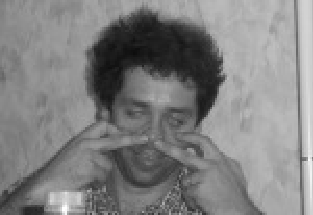
\includegraphics[width=3cm]{Fig_grim/serge_red}
\end{wrapfigure}
\vspace{-1cm}Mes premiers remerciements iront � mes  deux directeurs de th�se, tout
d'abord  Serge pour sa grande  disponibilit�, sa fonction {\it encyclo
de l'imagerie} � laquelle j'ai eu recours de nombreuses fois, pour son
appareil   photo num�rique aux   f�tes  d'�quipe (certains  pourraient
remettre en  question l'avantage d'instantan�it�  des appareils photos
num�riques...).
\begin{wrapfigure}{r}[\wrapdav]{3cm}
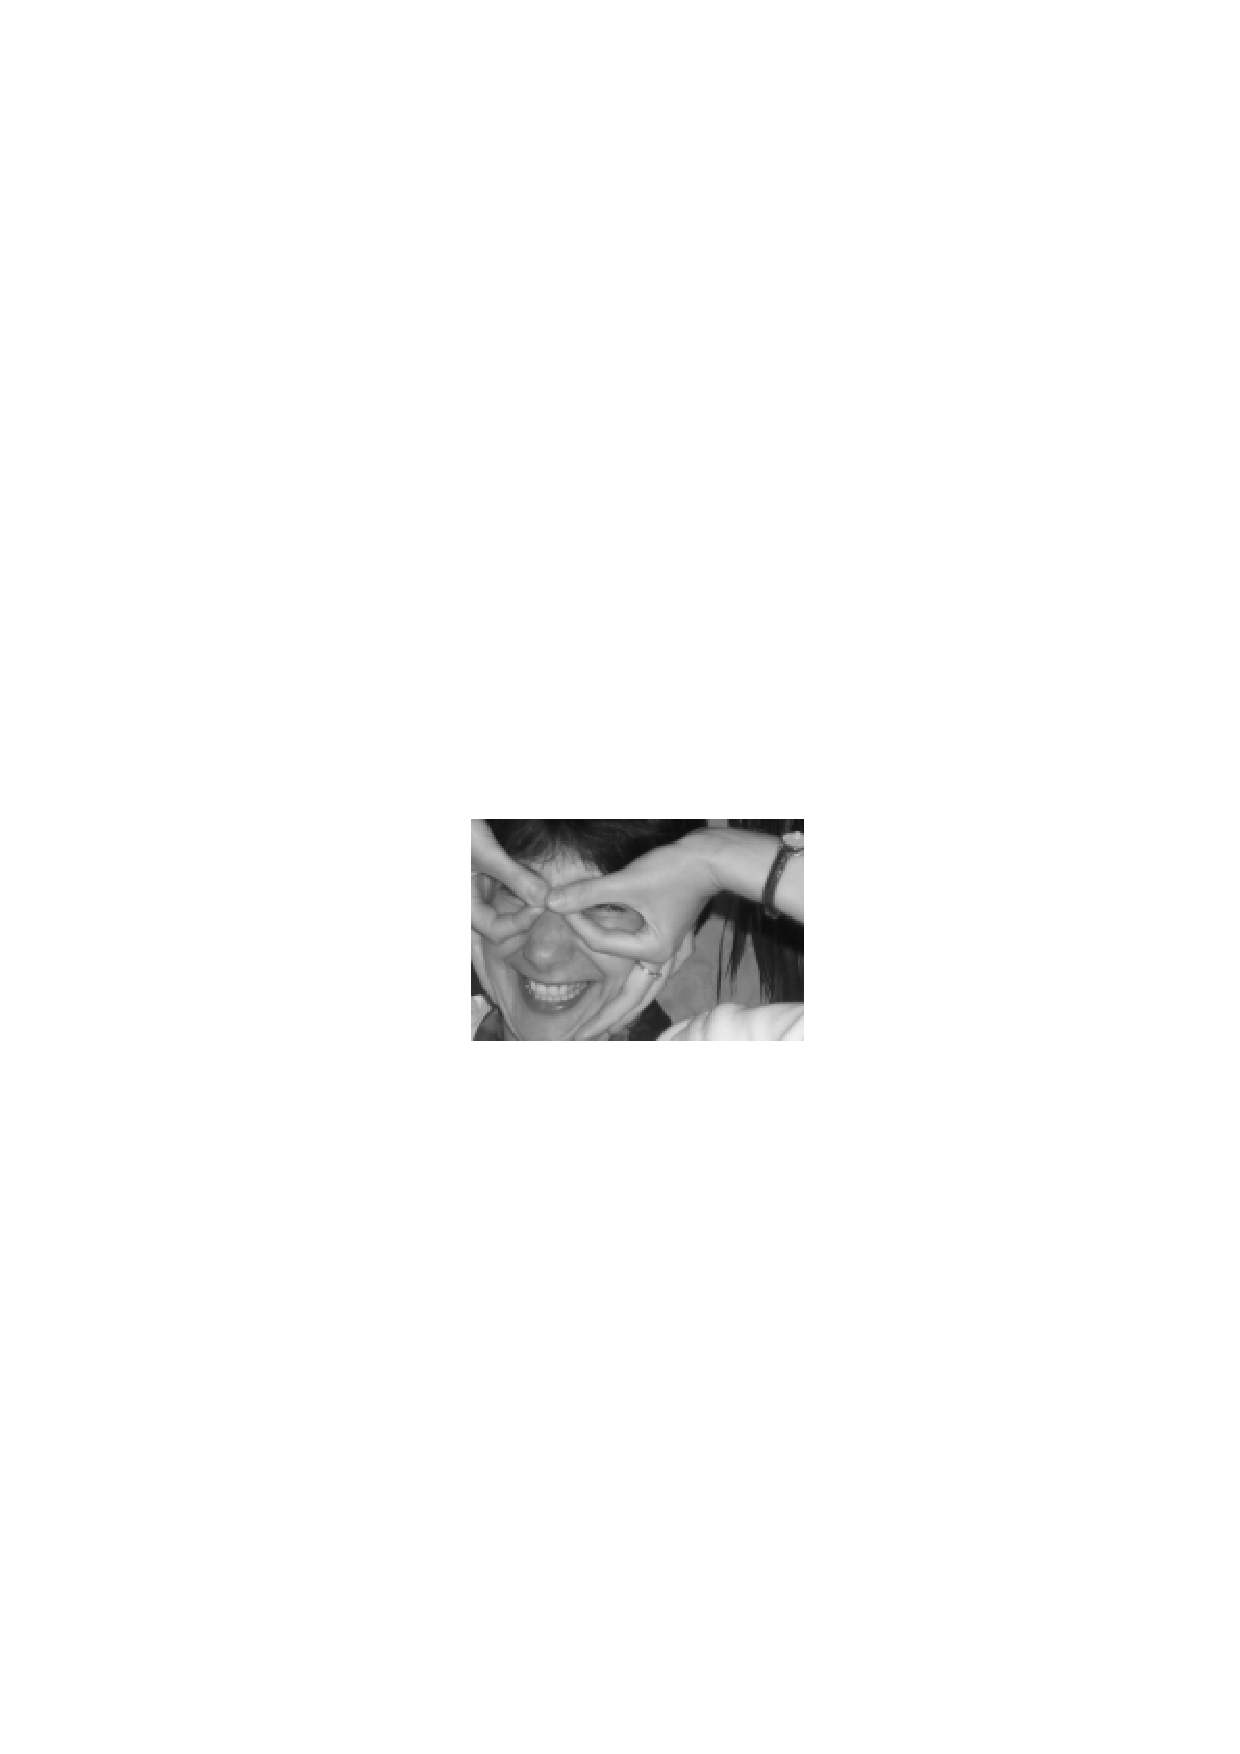
\includegraphics[width=3cm]{Fig_grim/laure_red}
\end{wrapfigure}
Un grand merci � Laure � qui je d�cerne le prix de {\it Correcteuse de
F�tes} en chef (sans elle, ce manuscrit aurait une forme de manuescry)
et  qui a d� me  supporter pendant trois  ans en face d'elle (�a fait
parfois mal aux oreilles...).

Je tiens  � remercier  Achille Braquelaire et Jean-Marc  Chassery
pour avoir  accept� de  rapporter sur   ce  looooonnng manuscrit. 
Je souhaiterais aussi remercier   Jean-Michel   Jolion d'avoir   bien  voulu
participer � mon jury de soutenance.

Un grand merci  � Jean-Pierre Reveill�s,  tout d'abord pour avoir fait
parti de mon  jury de soutenance, mais surtout  pour son accueil  tr�s
chaleureux. Je suis encore �tonn�  du grand int�r�t que Jean-Pierre  a
port� sur mes  premiers travaux alors  que j'�tais th�sard en premi�re
ann�e, d�couvrant le monde de la recherche  � un s�minaire � Dagstuhl.
Sa disponibilit� n'a   jamais   d�failli au cours de    nos nombreuses
rencontres en s�minaire ou en conf�rence.

Je tiens  �  remercier toutes  les personnes  que  j'ai rencontr�es en
conf�rences  ou en s�minaire.   De nombreux d�veloppements sont n�s de
ces rencontres.  Merci  donc � Isabelle (les deux),  Annick  (� qui je
dois une glace nougat-�rable), {\it the sweedish dream team} (Gunilla,
Stina et Ingela).  J'exprime aussi  toute ma reconnaissance � Reinhard
Klette pour la vision non   franco-fran�aise de la g�om�trie  discr�te
qu'il a su  m'apporter. Grand merci  � Jean-Bruno Brzoska,  � Fr�d�ric
Flin et  toute l'�quipe du CEN  de M�t�o-France pour m'avoir permis de
confronter mes   trucs  avec la  {\it   r�alit�}, ainsi que   pour les
discussions toujours tr�s int�ressantes que l'on a pu avoir.


Ensuite, derri�re  toute th�se il y  a un homme de l'ombre, technicien
des basses {\oe}uvres  (en gros  c'est du  deboggage  et des probl�mes
\LaTeX), le mien s'appelle David (aussi mais lui n'a pas encore vu la
beaut�  des  cubes... un jour  peut-�tre...)  et   je  le remercie bien
bas. Petit coucou aussi aux membres du labo ERIC pour l'ambiance qui y
r�gne,  en  vrac:  les Tweed-Clech  (Tiff   a  eu le   prix d'aspirante {\it
Correcteuse de F�tes}), les Scuturici, les  Jalam, Stephane et Fabrice
(mes potes de gal�re)\ldots

Pour   terminer, merci  �  la   famille pour  leur   support moral, en
particulier  � Jean-Fran�ois (toujours avoir un  fr�re stateux sous la
main...), et bien s�r � Anne (toujours avoir  une copine instit' sous la
main...).
\vspace{-0.5cm}\begin{flushright}
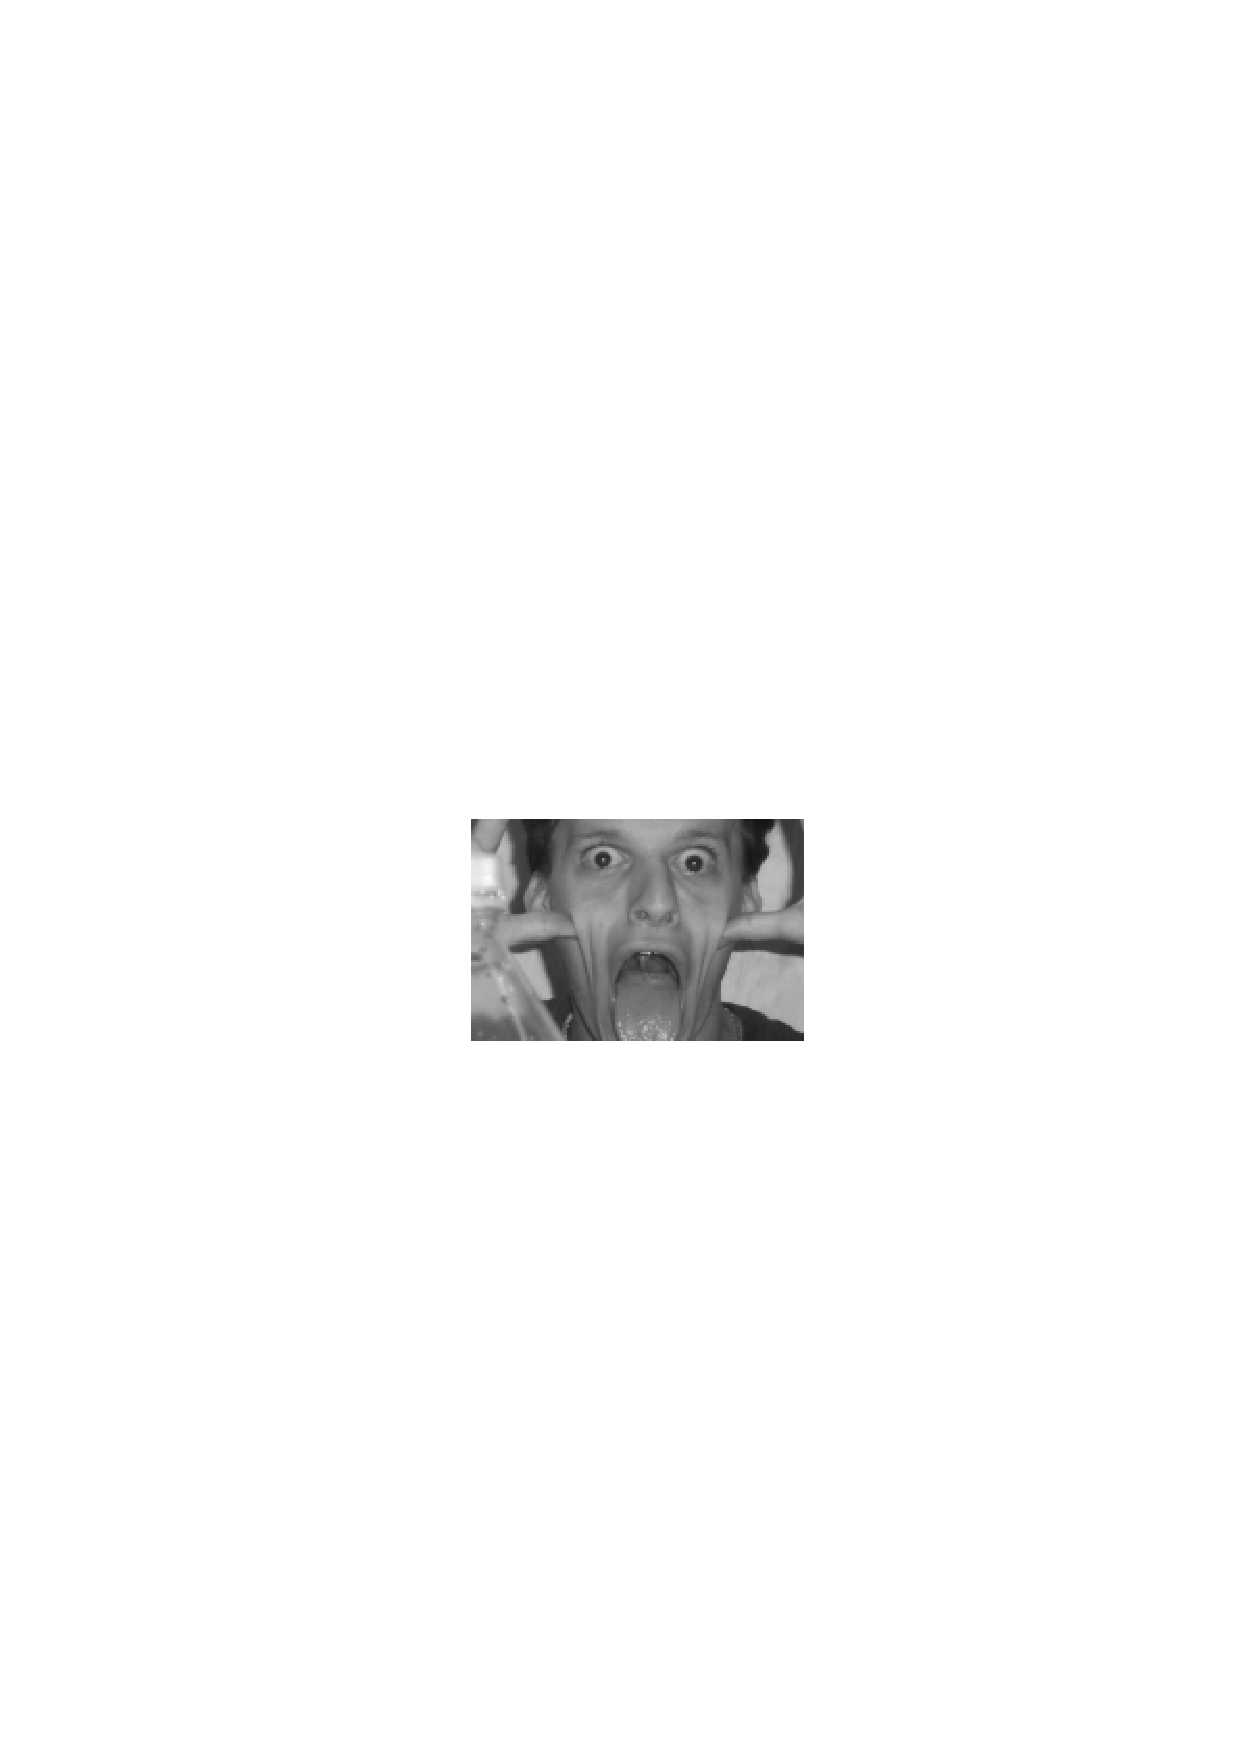
\includegraphics[width=3cm]{Fig_grim/dsarrut_red}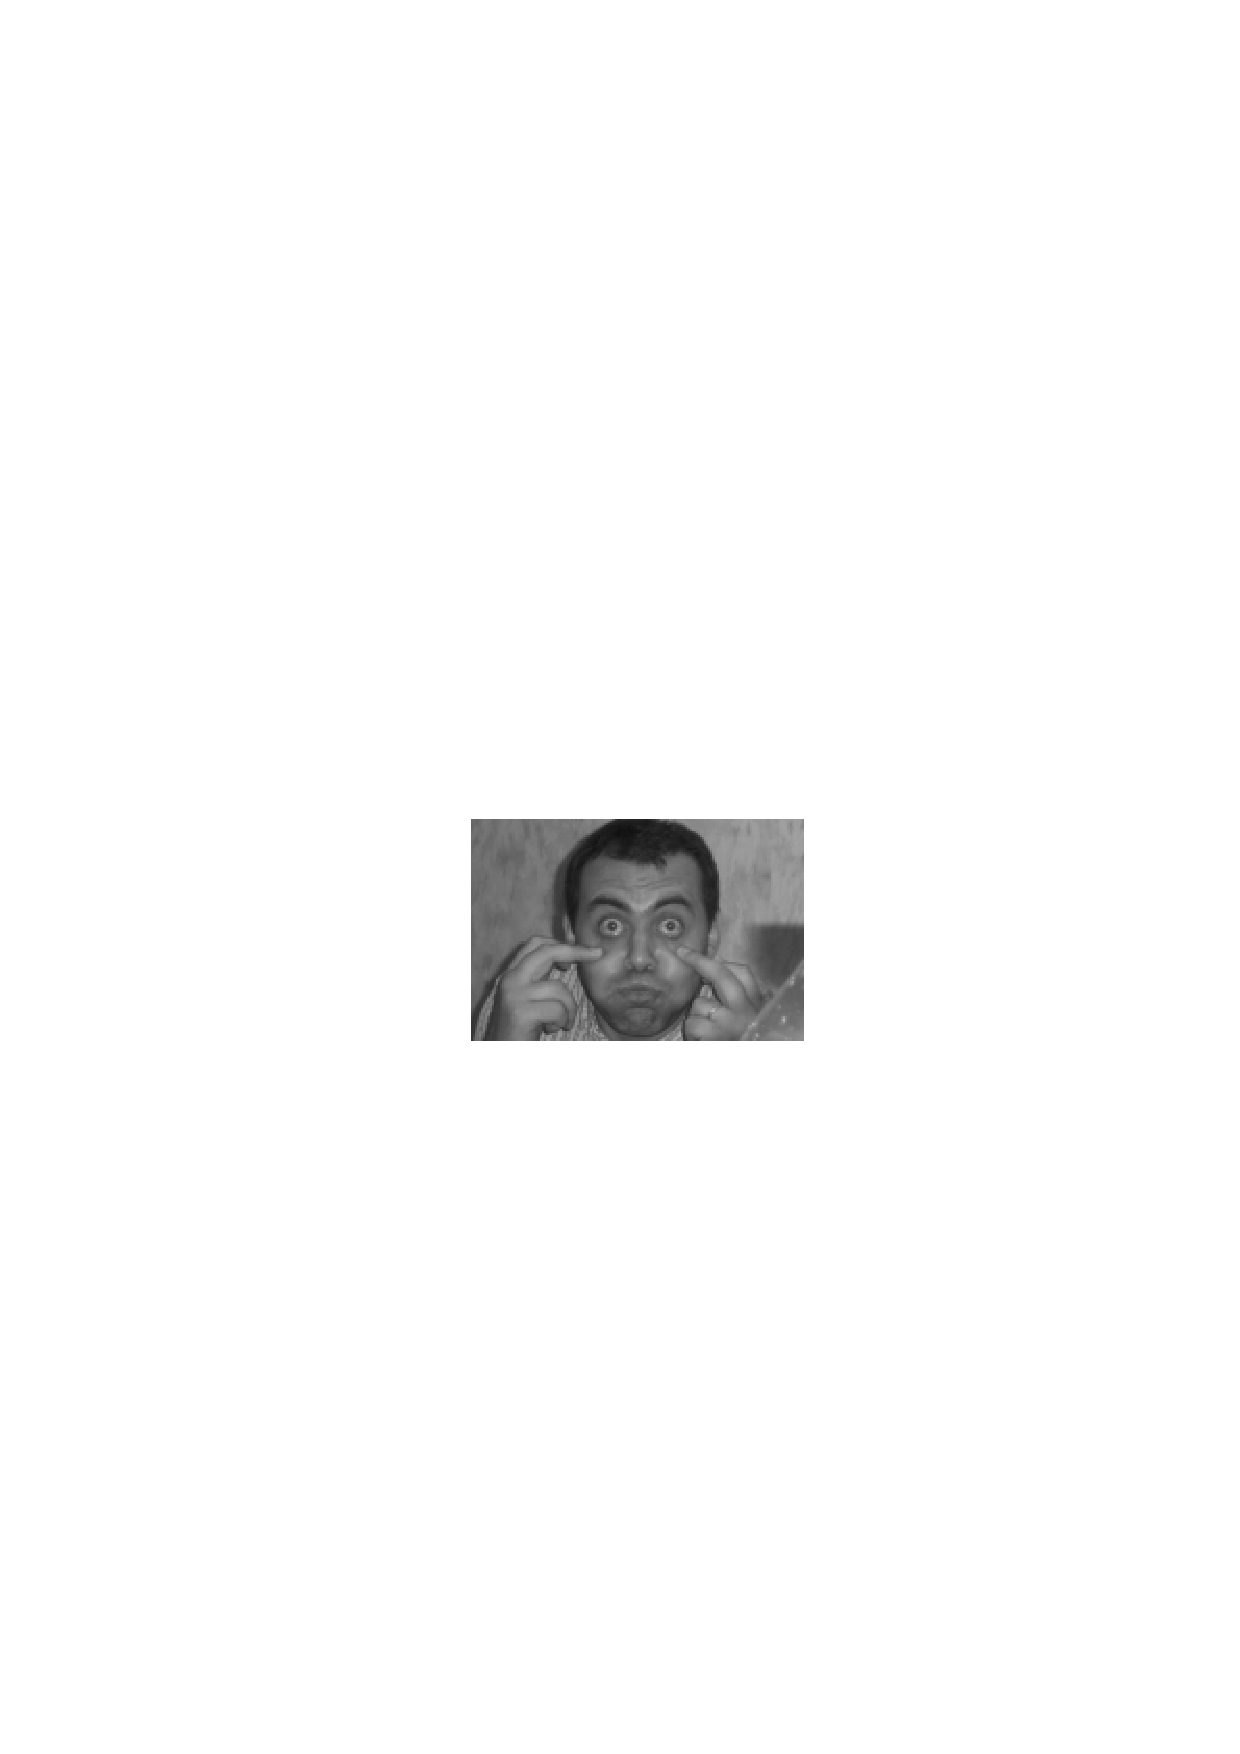
\includegraphics[width=3cm]{Fig_grim/marian_red}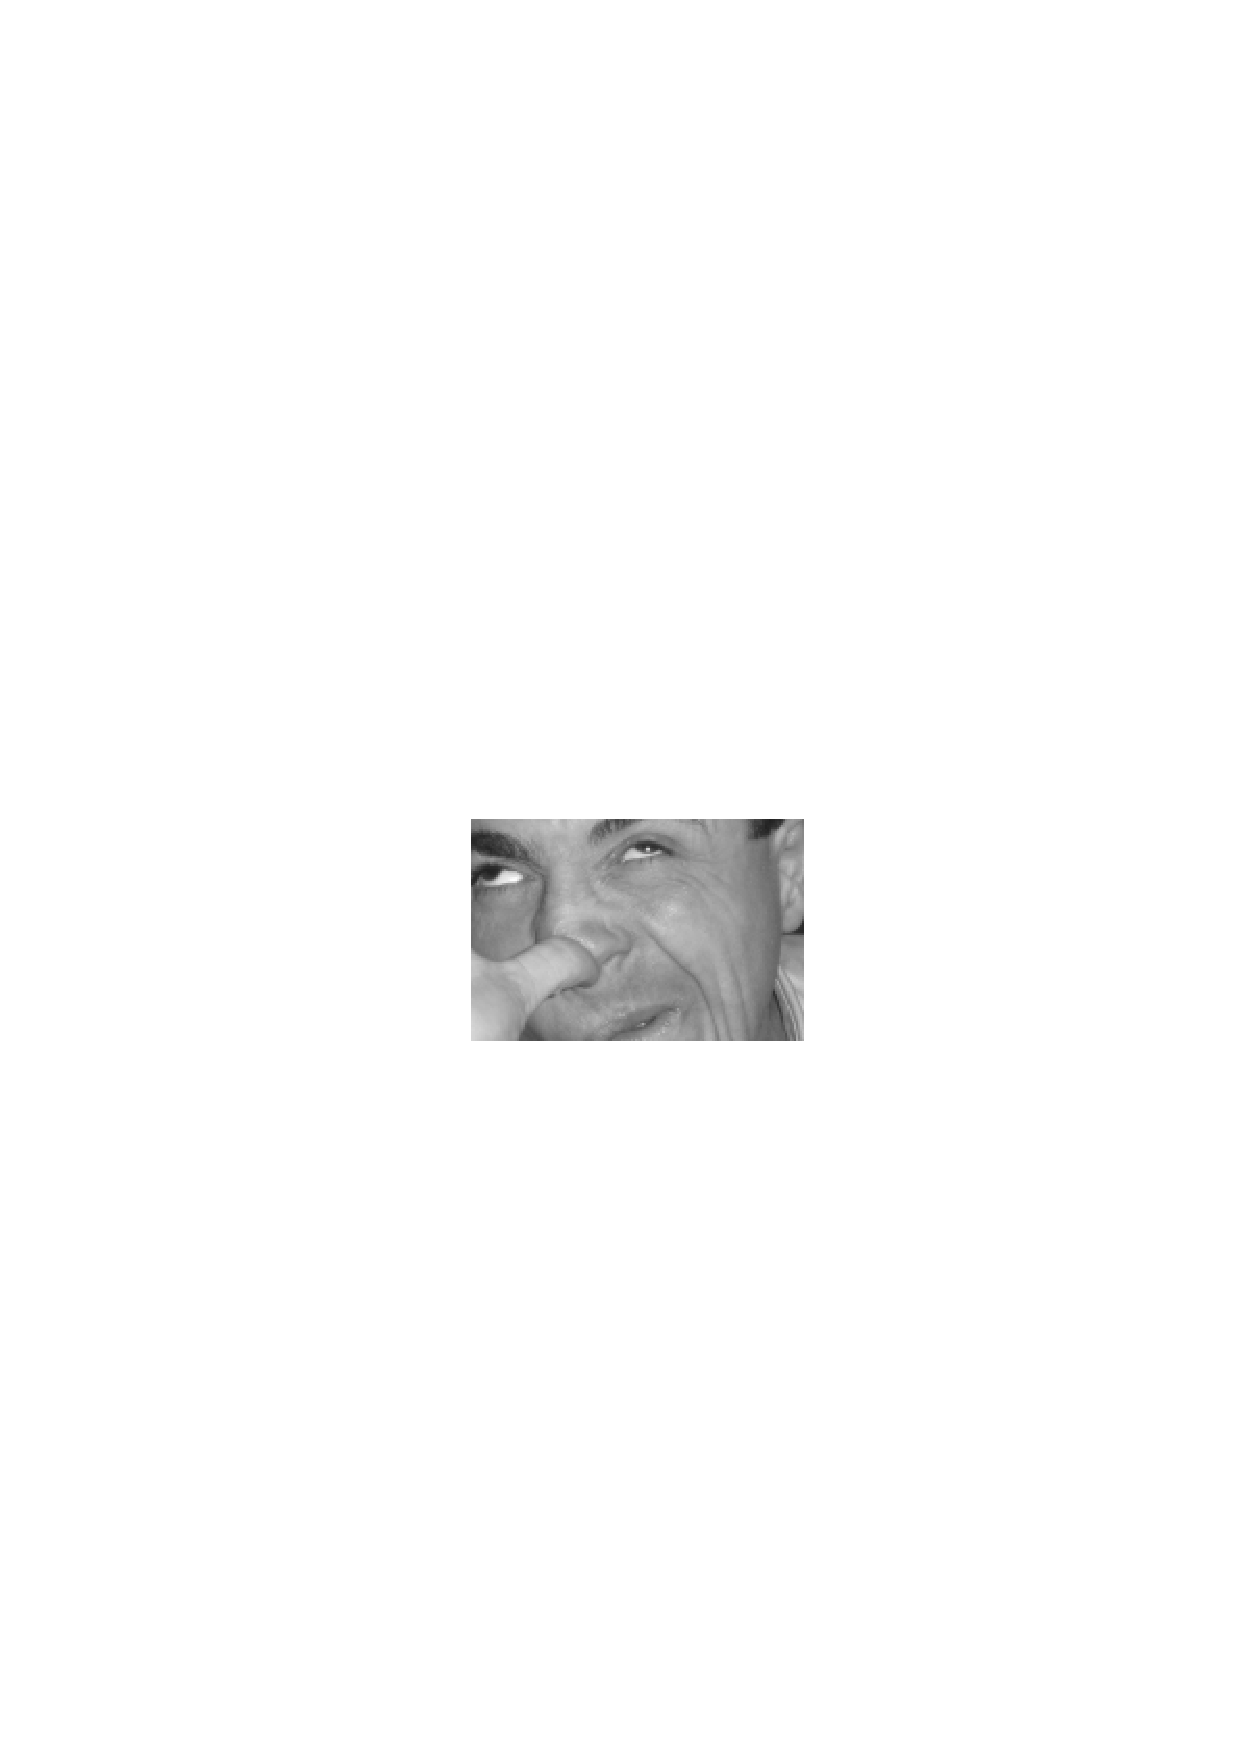
\includegraphics[width=3cm]{Fig_grim/seb_red}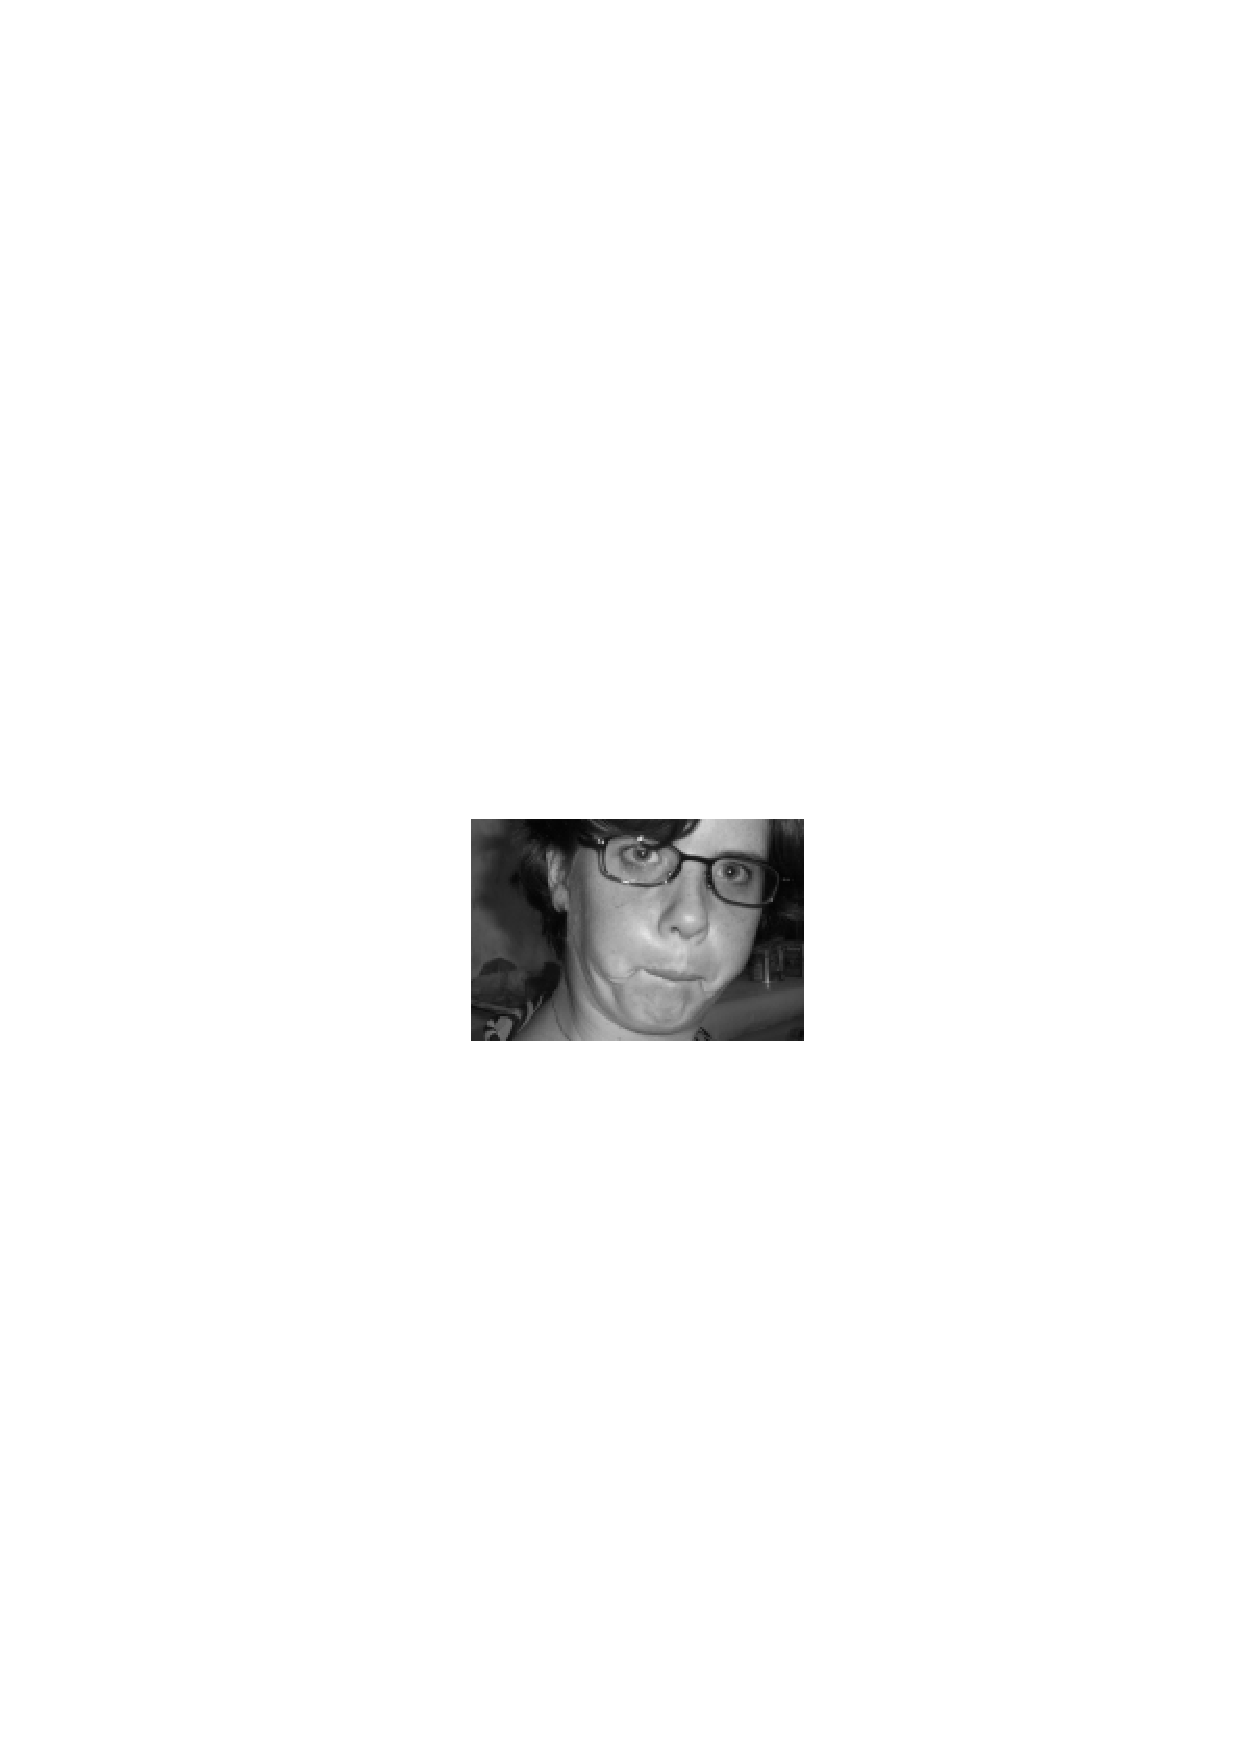
\includegraphics[width=3cm]{Fig_grim/anne_red}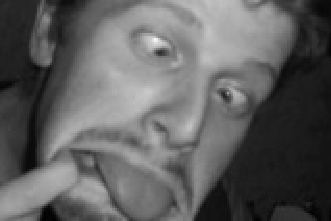
\includegraphics[width=3cm]{Fig_grim/dcoeurjo_red}
\end{flushright}


%%% Local Variables: 
%%% mode: latex
%%% TeX-master: "these"
%%% End: 

%%%%%%%%%%%%%%%%%%%%%%%%%%%%%%%%%%%%%%%%%%%%%%%%%%%%%%%%%%%%%%%%
\chapter*{R�sum�}

Cette  th�se  se situe  dans le  cadre  de  la g�om�trie  discr�te qui
constitue  l'une des grandes familles  de m�thodes d�di�es � l'analyse
automatis�e des formes  dans les images  num�riques 2D et 3D. Tous les
syst�mes d'acquisition d'images fournissent des donn�es organis�es sur
une  grille r�guli�re, appel�es  {\it donn�es discr�tes}. Les m�thodes
que nous nous proposons d'explorer et d'�tendre conservent aux donn�es
ce  caract�re discret, par opposition  aux techniques qui construisent
pr�alablement un mod�le continu approximant les objets � analyser.

Nous  nous int�ressons plus particuli�rement �  l'�tude des courbes et
des   surfaces discr�tes.  Dans un  premier  temps, nous analysons les
objets  de  base  que  sont  les  droites,  les plans  et  les cercles
discrets.  Nous pr�sentons  des  algorithmes  qui permettent de    les
caract�riser  et proposons des extensions   � ces m�thodes.   Ensuite,
nous    �tudions des m�triques  sur    les  objets discrets comme   la
transformation  en  distance euclidienne  ou   la notion de g�od�sique
discr�te.  Une approche bas�e sur   la  visibilit� dans les   domaines
discrets  est introduite.   La   troisi�me partie  est consacr�e �  la
d�finition et  �  l'�valuation  d'estimateurs de mesures  euclidiennes
telles  que  la longueur, la courbure  ou  l'aire.   Des  r�sultats de
convergence de ces estimateurs  sont �tablis.  Enfin, nous  pr�sentons
les applications dans  lesquelles  ces recherches ont  �t� utilis�es~:
classification   automatis�e d'objets  arch�ologiques  et  analyse des
micro-structures d'�chantillon de neige.


\paragraph{Mots cl�s~:} g�om�trie discr�te, analyse d'images, algorithmique.

%%%%%%%%%%%%%%%%%%%%%%%%%%%%%%%%%%%%%%%%%%%%%%%%%%%%%%%%%%%%%%%%
\chapter*{Abstract}

The context  of  the  work presented  in  this  thesis is the  digital
geometry.  This research area is devoted  to the automatic analysis of
objects in  digital images  in  dimension  2 and 3.    All acquisition
devices  provide data organized  on regular grids, called {\it digital
data}.   The  algorithms  that  are  explored  and  extended keep  the
discrete aspect of  the data, in opposition to  techniques based on an
approximation process of a continuous model.

More precisely, we  are interested in the  study of digital curves and
surfaces.  First of all,  we  consider basic  digital objects such  as
digital  straight lines, planes  and  circles.  We present  algorithms
that allow to characterize such objects and we propose some extensions
of these methods.  Then, we study some metrics  on the digital objects
such  as the Euclidean  distance transform  and  the notion of digital
geodesic.   An approach based   on the visibility property  in digital
domains is presented.    In the third  part,  we define and   evaluate
estimators of the Euclidean measurements such as the length, the curvature
or the area.  Some results on the  convergence of these estimators are
presented.  Finally, we illustrate some applications in which
these  researches have been  used for: archaeological object automatic
classification and snow sample micro-structure analysis.


\paragraph{Keywords:} digital geometry, image analysis, algorithmic.


%%% Local Variables: 
%%% mode: latex
%%% TeX-master: "these"
%%% End: 
% LocalWords:  int�grables Remote Access Medical Imaging System




\setlength{\parskip}{1mm} % Espace inter par ici pour que TOC soit OK 
\tableofcontents
\listoffigures
\listoftables
\listofalgorithms
%%%%%%%%%%%%%%%%%%%%%
%%%%%%%%%%%%%%%%%%%%%%%%%%%%%%%%%%%%%%%%%%%%%%%%%%%%%%%%%%%%%%%%%%%%
%\chapter*{Introduction\\\rule{\textwidth}{0.1cm}}
\chapter*{Introduction\vspace{1mm}\hrule}
\addcontentsline{toc}{starchapter}{Introduction}
\thispagestyle{plain}
\markboth{Introduction}{Introduction}
\pagenumbering{arabic}
\setcounter{page}{1}
%%%%%%%%%%%%%%%%%%%%%%%%%%%%%%%%%%%%%%%%%%%%%%%%%%%%%%%%%%%%%%%%%%%%


Tous   les syst�mes  d'acquisition de  donn�es  images fournissent des
donn�es  organis�es sur  une  grille r�guli�re, appel�es {\it  donn�es
discr�tes}.  Que ce  soit pour une  visualisation ou pour l'extraction
de mesures sur ces objets discrets (param�tres de formes), les axiomes
et th�or�mes  de   la g�om�trie euclidienne  ne  sont  pas directement
applicables.  Deux solutions s'offrent � nous.  La premi�re consiste �
plonger les donn�es discr�tes dans un  espace continu o� ces th�or�mes
et mesures    sont d�finis (par exemple   en   utilisant des processus
d'interpolation).  Une seconde alternative   se base sur  une transposition de
ces th�or�mes   et mesures dans    l'espace discret.  Ces  diff�rentes
re-d�finitions     donnent lieu    �  un    paradigme math�matique  et
informatique appel� {\it g�om�trie discr�te}.

Un premier int�r�t  d'une telle d�finition  est que nous �vitons ainsi
un  changement  de mod�le co�teux en   temps et potentiellement source
d'impr�cisions.  Dans le cadre   de  la g�om�trie  algorithmique,  les
erreurs  d'arrondi engendr�es par  de  tels processus peuvent affecter
non  seulement les   r�sultats mais   aussi   la terminaison m�me   de
l'algorithme.   Dans    l'introduction   de   la   th�se    d'�tat  de
\aut{Jean-Pierre} \cite{reveilles}, nous pouvons lire~:

\begin{quote}
{\it  De fa�on g�n�rale, d�s que des donn�es ont  �t� tronqu�es plus aucun
  th�or�me   g�om�trique n'est   vrai.   On peut   dire alors  que  la
  g�om�trie, qui, sur  le papier, �tait  d�j� l'art de raisonner juste
  sur des figures fausses,  devient,  sur machine, l'art de  raisonner
  juste � partir de calculs   faux produisant des figures fausses,  si
  toutefois les calculs terminent.}
\end{quote}

D'un  point de vue  algorithmique, l'analyse  de  ces  objets sur  une
grille   r�guli�re � l'aide   d'une  m�thodologie  en nombres  entiers
permet, non seulement une   gestion  de ces incertitudes,  mais  aussi
l'�criture d'algorithmes tr�s   efficaces.   En effet,  comme  nous le
verrons par la suite, la manipulation de  nombres entiers et les liens
tr�s forts  entre les objets discrets  et des th�or�mes de  la th�orie
des    nombres  ou     d'arithm�tique    offrent   des    possibilit�s
d'impl�mentations d'outils g�om�triques tr�s efficaces.

Derri�re ces consid�rations  d'ordre  th�orique  se cache  un  int�r�t
pratique tr�s  important.  En  effet, une  th�orie g�om�trique  et une
algorithmique   adapt�e  aux images  nous   permettent d'acc�l�rer les
processus   mais surtout de  proposer des  outils  d'analyse de formes
coh�rents avec la modalit� des objets analys�s.

Cet  int�r�t pratique a �t� illustr�  depuis tr�s longtemps. Ainsi, en
1771, en pr�sentant un principe  d'interpolation lin�aire bas� sur des
entiers  et  sur des    modulos (ce  qui   correspond  exactement  aux
fondements des droites  discr�tes), \aut{Jean Bernouilli}  conclut son
article avec la  certitude d'avoir pr�sent�  une technique  qui allait
�tre un outil de base de la g�om�trie discr�te contemporaine~:

\begin{quote}
{\it [...]  je  me  flatte de   mettre  sous les yeux   des astronomes
diff�rentes m�thodes  d'abr�ger consid�rablement leurs calculs, qu'ils
ne connaissaient pas  encore, ou que,  par des  raisons qui cesseront,
ils ont n�glig� de saisir lorsqu'elles leur ont �t� pr�sent�es pour la
premi�re fois ; [...]  }
\end{quote}



Les recherches pr�sent�es dans ce manuscrit s'inscrivent dans ce cadre
de la g�om�trie discr�te  et concernent plus particuli�rement  l'�tude
des courbes et des surfaces discr�tes.

\section*{Organisation du manuscrit}

Ce manuscrit est d�compos� en trois parties~: la premi�re concerne les
notions de base et les diff�rents objets du mod�le discret. La seconde
s'int�resse � l'analyse de  formes   et aux  mesures sur  ces   objets
discrets.  Enfin, la     troisi�me partie correspond  aux   annexes.

Plus   pr�cis�ment, apr�s avoir pr�sent�  quelques  notions de base en
g�om�trie utiles pour la suite, nous analysons les  objets de base que
sont les droites, les plans et les cercles discrets, et pr�sentons les
algorithmes qui permettent  de les caract�riser.  En particulier, nous
proposons   une  synth�se des    diff�rentes approches et  algorithmes
associ�s aux droites discr�tes en dimension 2  et 3. Nous reprenons ce
travail bibliographique sur   les   plans discrets en    proposant une
premi�re caract�risation    de la pr�-image   d'un morceau    de  plan
discret. Nous concluons ce  chapitre sur les droites  et les plans par
une analyse statistique de ces objets.

Nous nous int�ressons par la suite aux notions  de cercles discrets et
aux diff�rents  algorithmes de reconnaissance associ�s. Nous proposons
dans ce chapitre un algorithme de reconnaissance  de cercle discret et
de segmentation d'une courbe  discr�te en arcs  de cercle bas� sur une
r�solution arithm�tique du probl�me.

Dans  la seconde  partie, nous  utilisons  cette analyse des objets de
base pour caract�riser des  formes ou des contours  de formes.  Ainsi,
nous  pr�sentons un  algorithme de calcul  de  transform�e en distance
euclidienne sans erreur  bas� sur la  notion  de diagramme  de Vorono�
discret.   En utilisant ce  diagramme particulier, nous pr�sentons des
premi�res pistes vers  une extraction de  squelette de forme.  Dans ce
m�me chapitre, nous proposons une d�finition de la visibilit� discr�te
dans des domaines discrets non-convexes bas�e sur  la notion de droite
discr�te.  Cette d�finition de la visibilit�  nous permet par la suite
de proposer un calcul de chemins g�od�siques discrets.

Ensuite, nous nous  int�ressons aux   re-d�finitions, dans le   mod�le
discret, de mesures euclidiennes.   En utilisant le cadre th�orique de
la convergence  asymptotique, nous  pr�sentons diff�rents  algorithmes
permettant  d'estimer la longueur d'une  courbe discr�te, les normales
en tout point de cette courbe et la  courbure associ�e � chaque pixel.
Dans  le  cas  des   surfaces  discr�tes, nous   proposons  diff�rents
estimateurs  permettant d'estimer l'aire  de la  surface, les vecteurs
normaux en  tout point  et   une estimation de   diff�rentes courbures
(moyenne et gaussienne).


 
Finalement,  la derni�re partie correspond  aux annexes et contient un
premier  chapitre   pr�sentant les diff�rentes   applications  qui ont
inspir�  ces    d�veloppements th�oriques,   un  second  contenant les
diff�rentes preuves de  convergence asymptotique ainsi qu'un troisi�me
d�taillant un algorithme de  programmation lin�aire que nous utilisons
dans les parties pr�c�dentes.

La figure  \ref{fig:plan_these}  pr�sente les diff�rentes  d�pendances
entre ces chapitres et parties.  Par  exemple, les notions introduites
dans  le chapitre sur les droites   et plans discrets seront utilis�es
pour construire des     estimateurs de mesures euclidiennes   et  nous
permettent de d�finir la notion de visibilit� discr�te.

Une  lecture   lin�aire des chapitres   de  ce manuscrit est possible,
cependant  nous pouvons conseiller au   lecteur de commencer par  le chapitre
relatant les  diff�rentes applications (annexe \ref{chap-app}) afin de
d�buter par ce qui a motiv� nos recherches.


\begin{figure}[htbp]
  \centering
  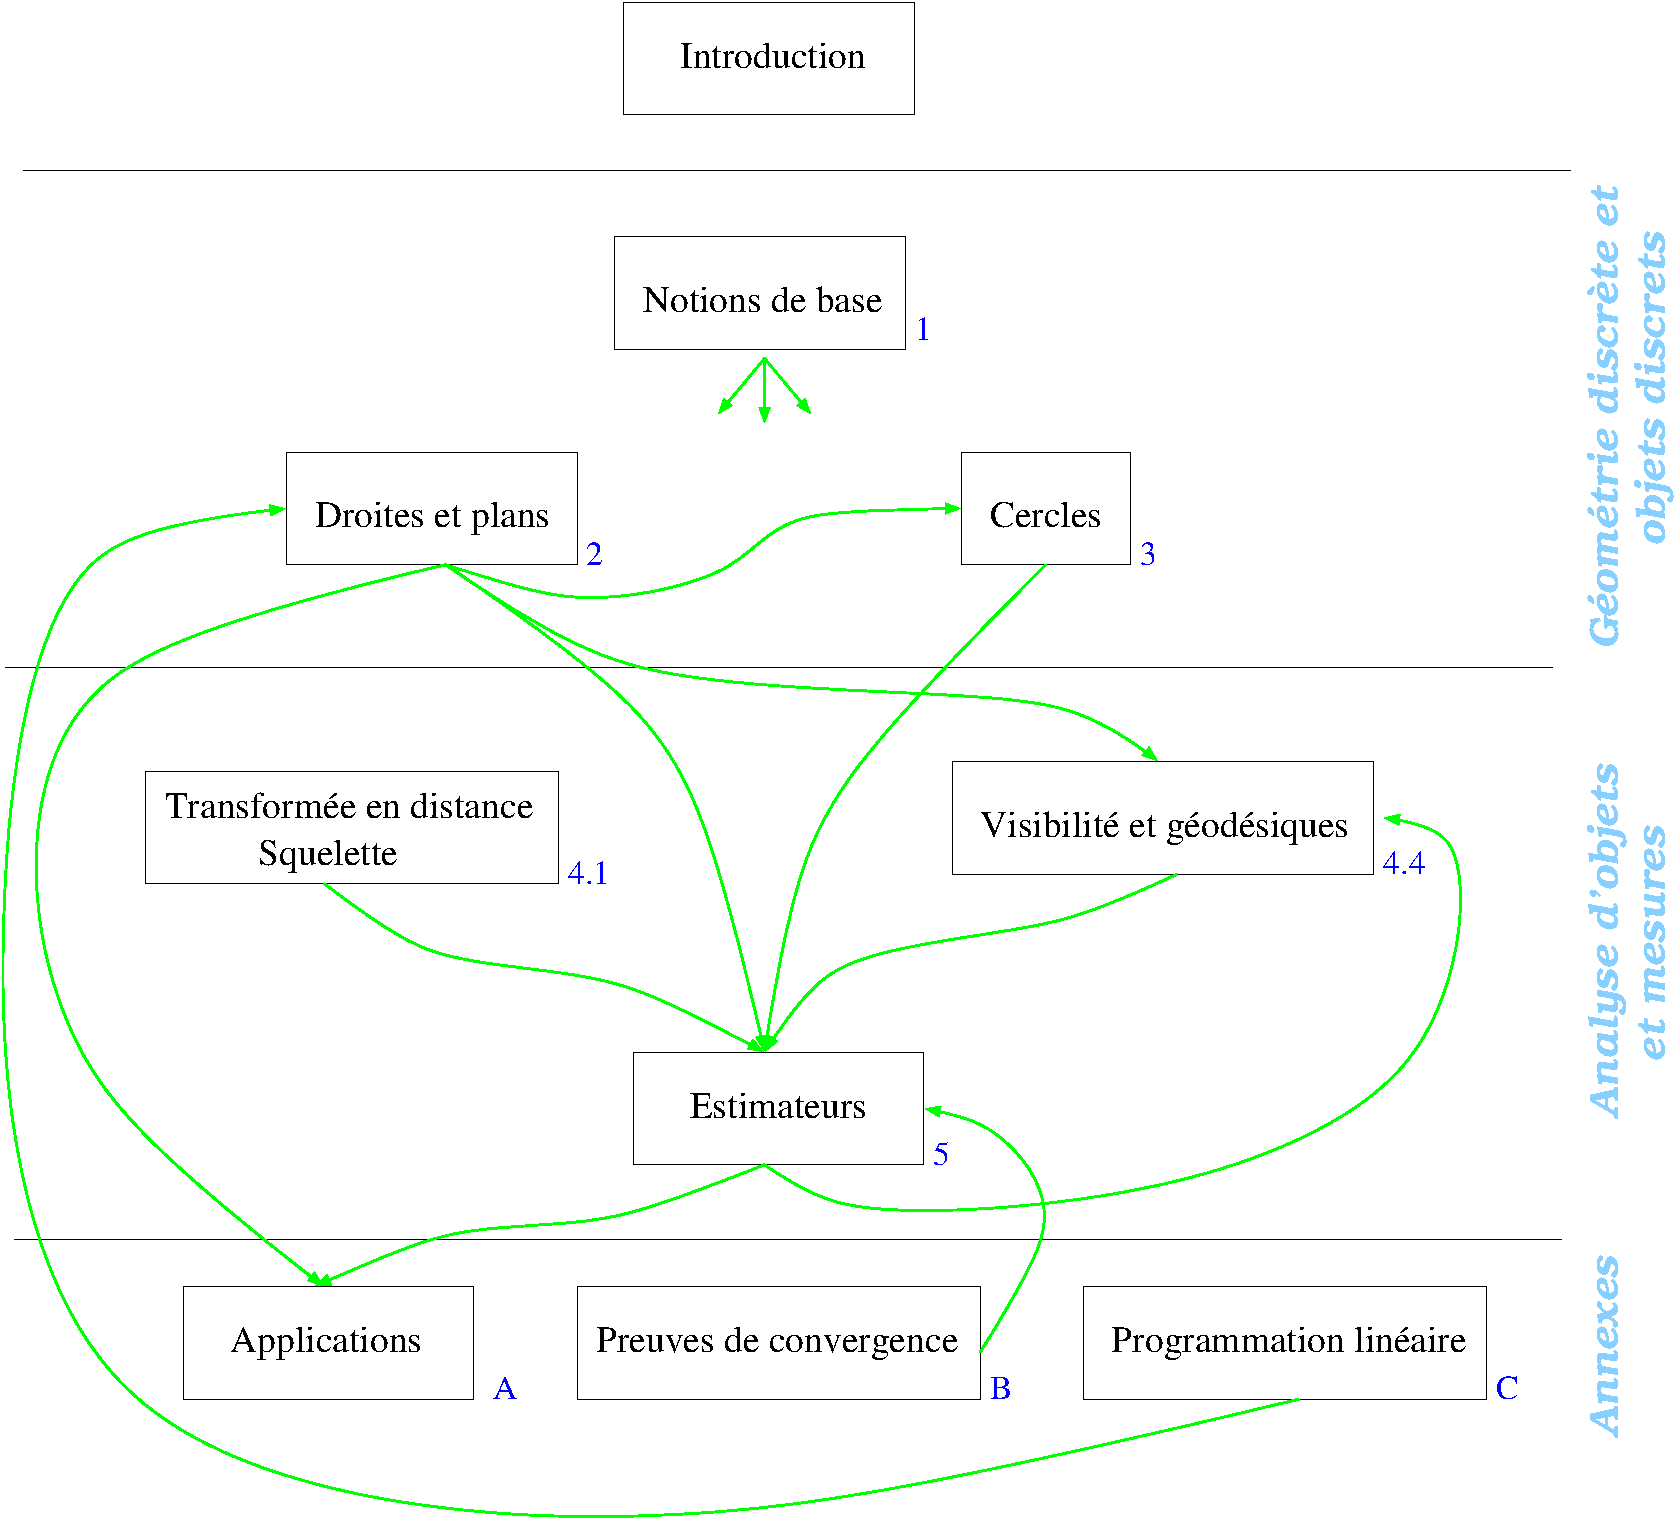
\includegraphics[width=14cm]{plan_these}
  \caption{Organisation du manuscrit,   les fl�ches
    indiquent les d�pendances entre chapitres.}
  \label{fig:plan_these}
\end{figure}




%%% Local Variables: 
%%% mode: latex
%%% TeX-master: "these"
%%% End: 


\stepcounter{mtc} %pour eviter l{\'\i}ntro

\part[G{\'e}om{\'e}trie discr{\`e}te et objets
discrets]{G{\'e}om{\'e}trie discr{\`e}te et objets discrets \\
  \vspace*{2cm} \protect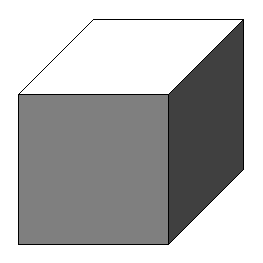
\includegraphics[width=4cm]{CUBE} \\
  \protect\flushright{\it {\LARGE Ceci est~:~~~~~\hspace*{5cm}} \\{\large un morceau de droites
    discr�tes\\un morceau de plan discret\\ un morceau de cercle
    discret\\parfois un simple cube mais c'est plus rare\ldots}}}
%\part{Objets}

%%%%%%%%%%%%%%%%%%%%%%%%%%%%%%%%%%%
\mychaptoc{Notions de base}\label{chap-notions}
 %%%%%%%%%%%%%%%%%%%%%%%%%%%%%%%%%%

\section{Introduction}

Dans ce chapitre, nous introduisons certaines notions et propri�t�s de
bases   de la g�om�trie  discr�te.   Celles-ci seront utilis�es par la
suite pour d�finir   diff�rents objets et  algorithmes sur  la  grille
discr�te.

\section{Espace discret et connexit�}

Nous commen{\c c}ons   par d�crire les  notions de  base  en g�om�trie
discr�te  (voir  \citealt{montanvert}).   Nous appelons  {\it   espace
discret} par la suite  un pavage r�gulier du   plan en dimension  2 ou
plus   g�n�ralement de l'espace en  dimension  sup�rieure (voir figure
\ref{fig:pavage}).    Nous appelons aussi    un {\it point discret} le
centre de gravit� de chaque cellule dans le pavage consid�r�.

\begin{figure}[htbp]
\begin{center}
  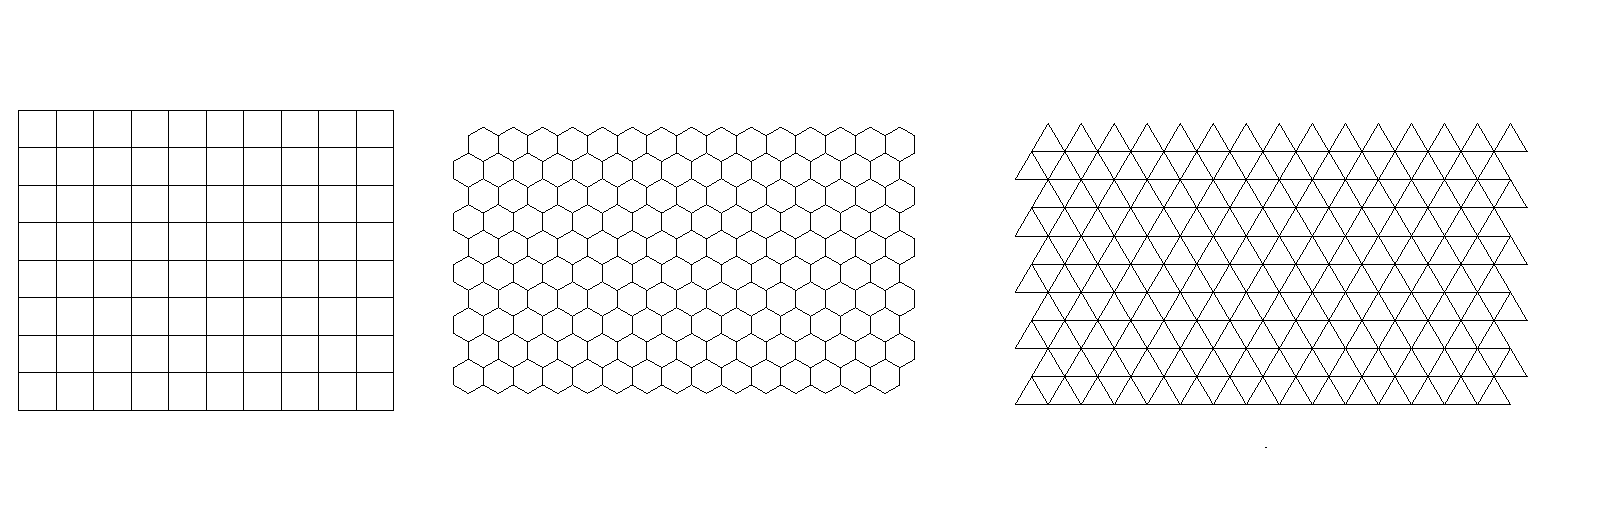
\includegraphics[width=15cm]{pavage.eps}
  \caption{Pavages r�guliers en dimension 2 par carr�s, par hexagones  et par
    triangles}
  \label{fig:pavage}
\end{center}
\end{figure}

Dans ce qui  suit, nous  repr�sentons graphiquement l'espace  discret,
soit par le  pavage r�gulier, soit par le  maillage issu de ce  pavage
qui est un graphe  dont les sommets sont  les points discrets et  dont
les  ar{\^e}tes repr�sentent  les  adjacences des  �l�ments  du pavage
(voir figure \ref{fig:maillage}).

\begin{figure}[htbp]
\begin{center}
  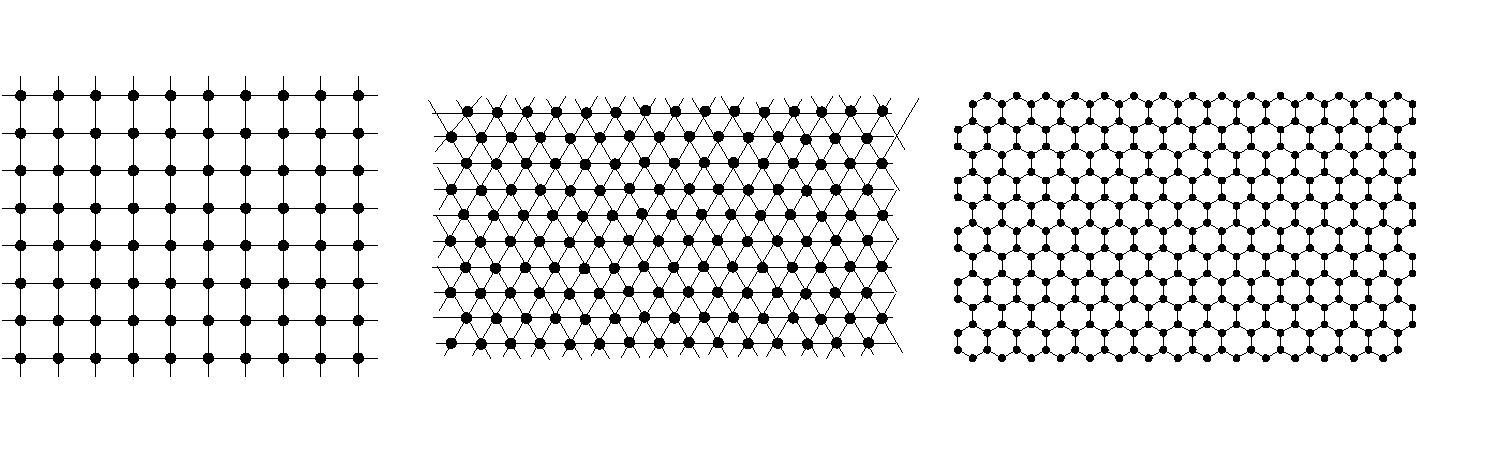
\includegraphics[width=15cm]{maillage}
  \caption{Repr�sentation duale par maillage en dimension 2.}
  \label{fig:maillage}
\end{center}
\end{figure}

En g�om�trie discr�te, les espaces discrets engendr�s par des carr�s ou des
cubes multi-dimensionnels pour les dimensions sup�rieures, sont les plus
utilis�s. Les points discrets associ�s {\`a} ces espaces sont donc des
points de $\Z^n$ pour la dimension $n$.

Sur cet espace discret, nous introduisons des notions de {\it
  voisinage} nous permettant de construire des graphes
d'adjacence. Ainsi, si nous consid�rons un espace discret 2D g�n�r�
par des carr�s, nous d�finissons le {\it 4-voisinage} comme �tant la
relation d'adjacence par ar{\^e}tes  dans la partition de l'espace et le
{\it 8-voisinage} comme �tant la relation d'adjacence par ar{\^e}tes et par
sommets. Plus formellement, deux points $p$ et $q$ de $\Z^2$ sont {\it
  4-voisins}  (ou {\it 4-adjacents}) si :
\begin{displaymath}
  |x_p - x_q| + |y_p - y_q| =1
\end{displaymath}

De la m{\^e}me mani�re, deux points $p$ et $q$  de $\Z^2$ sont {\it
  8-voisins}  (ou {\it 8-adjacents}) si :
\begin{displaymath}
  max(|x_p-x_q|,|y_p-y_q|)=1
\end{displaymath}


En dimension 3, nous pouvons introduire les notions de {\it 6-, 18-} ou
{\it 26-voisinage} en consid�rant les adjacences par faces, par ar{\^e}tes et
par sommets (voir figure \ref{fig:adjacences3D}). Ces adjacences
peuvent s'�crire formellement :




\begin{center}
  \begin{tabular}{|l|r|}
    \hline
    adjacence & caract�risation \\
    \hline
    $6$ &  $|x_p - x_q| + |y_p - y_q| + |z_p - z_q|=1$\\
    $18$ & $p$ et $q$ sont 26-voisins et $|x_p - x_q| + |y_p - y_q| +
    |z_p - z_q| \leq 2$\\
    $26$ & $max(|x_p-x_q|,|y_p-y_q|,|z_p - z_q|)=1$\\
    \hline
  \end{tabular}
\end{center}

\begin{figure}[htbp]
\begin{center}
  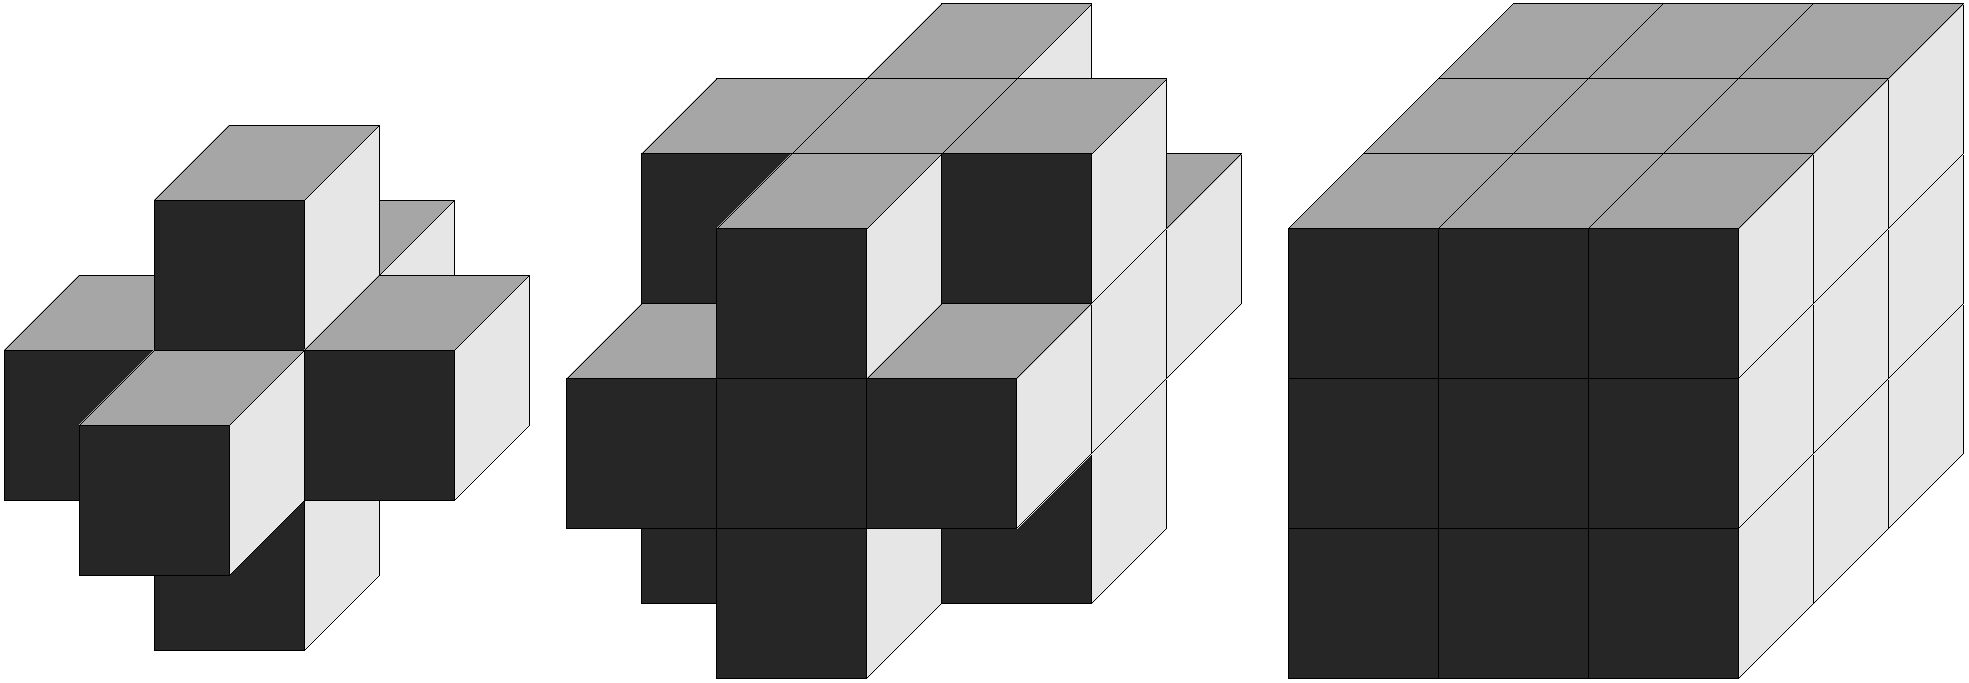
\includegraphics[width=8cm]{connexite}
  \caption{Diff�rentes connexit�s en 3D sur un pavage par cubes.}
  \label{fig:adjacences3D}
\end{center}
\end{figure}

En  dimension $n$, une �criture  unifi�e  de ces diff�rentes relations
d'adjacence s'exprime sous la   forme de {\it O(r)-voisinage}  : deux
points  de $\Z^n$ sont   {\it  O(r)-voisins} si leurs  coordonn�es  ne
diff�rent que de  1 et qu'au moins $n-r$  coordonn�es sont �gales (voir
\citet{jonas97} par exemple). Ainsi, les connexit�s 6,  18 et 26 en 3D
s'�crivent respectivement $O(1)$, $O(2)$ et $O(3)$ dans ce
sch�ma (voir table \ref{tab:vois} pour une comparaison des
diff�rentes notations).


\begin{table}[htbp]
  \begin{center}
    \begin{tabular}{|c|c|c|c|}
      \hline
      $O(r)$-voisinage &       \multicolumn{3}{|c|}{$k-$voisinage}\\ \cline{2-4}
      
       &  $2D$ & $3D$ & $nD$\\
       \hline
       1 & 4 & 6 & $2n$\\
       2 & 8 & 18 & $2n^2$\\
       3 & . & 26 & \ldots\\
       \ldots& . &. & \ldots\\
       $r$ & . & . & $\sum_{i=n-r}^{n-1} \frac{n!}{i!(n-i)!}2^{n-i} $\\
      \ldots& . &. & \ldots\\
      $n$ & . & . & $3^n -1$\\
      \hline
    \end{tabular}
    \caption{Liens entre notations de voisinage pour un pavage  par hypercubes.}
    \label{tab:vois}
  \end{center}
\end{table}

Dans  le cas d'un pavage  hexagonal,  nous n'avons  qu'un seul voisinage
�l�mentaire appel� {\it 6-voisinage}. Pour une grille triangulaire,
nous pouvons d�crire, avec les m{\^e}mes principes que pr�c�demment, le
{\it 3-voisinage} (connexit� par ar{\^e}te) et le {\it 12-voisinage}
(connexit� par ar{\^e}tes et par sommets). 

\section{Objets, courbes, surfaces et hyper-surfaces}

Maintenant  que l'espace de travail  est d�fini,  nous pouvons d�crire
les objets que l'on manipulera par la suite. Bien �videment, la notion
de courbe  ou de surface est intimement  li�e aux notions topologiques
que nous introduirons sur l'espace discret.

Dans un premier temps, les relations d'adjacence d�crites pr�c�demment
permettent de d�finir un {\it k-chemin} sur l'espace discret : 

\begin{defi}[$k-$chemin]
  Soit un ensemble $\E$ de points discrets   et une relation de
  $k-$adjacence, $\E$ est un $k-$chemin si pour tous les
  �l�ments $\{p_i\}_{i=0..n}$ de $\E$, $p_i$ est $k-$voisin de $p_{i-1}$.
\end{defi}


Nous pouvons d�finir de la m{\^e}me mani�re un objet dans un espace
discret muni d'une relation d'adjacence.

\begin{defi}[$k-$objet]
  Soit un ensemble $\E$ de points discrets et une relation de
  $k-$adjacence, $\E$ est un $k-$objet si pour tout couple $p$ et $q$
  de $\E$, il existe un $k-$chemin dans $\E$.
\end{defi}

Selon une approche orient�e graphe, un $k-$objet peut-{\^e}tre vu
comme une composante connexe dans le graphe dont les sommets sont les
points discrets et les ar{\^e}tes les $k-$adjacences \citep{Rosenfeld1970}.

La notion de $k-$chemin d�crite ci-dessus est tr�s g�n�rale. Nous
restreignons cette notion pour pouvoir introduire des propri�t�s
topologiques sur ces objets. Nous proposons ainsi la notion de
$k-$arc d�finie par \citet{rosenfeld}.

\begin{defi}[$k-$arc]
  Soit  un  ensemble $\E$  de  points  discrets  et  une relation   de
  $k-$adjacence,  $\E$    est un $k-$arc si     pour tous les �l�ments
  $\{p_i\}_{i=0..n}$    de  $\E$,   $p_i$   a  exactement  deux points
  $k-$voisins, sauf $p_0$ et $p_n$ appel�s alors extr�mit�s de l'arc.
\end{defi}


Si le $k-$arc est ferm�  on parle alors de $k-$courbe. 


\begin{defi}[$k-$courbe]
  Soit un ensemble $\E$ de points discrets  et une relation de
  $k-$adjacence, $\E$ est une $k-$courbe si $\E$ est un $k-$arc et que
  $p_0=p_n$.
\end{defi}

Pour simplifier l'�criture,  nous utiliserons le terme g�n�rique  {\it
courbe discr�te} pour repr�senter une $k-$courbe ou un $k-$arc.

L'introduction des courbes l�ve des  probl�mes topologiques. En effet,
une  propri�t� {\it  souhaitable} sur une   $k-$courbe serait que l'on
puisse  d�finir un int�rieur et   un ext�rieur. Ces d�finitions  sont li�es
{\`a} la  notion de  propri�t� de  Jordan  en g�om�trie diff�rentielle
classique que nous d�taillerons dans la section suivante.


\subsection{Notions de topologie discr�te}
\label{sec:topo}

En g�om�trie diff�rentielle classique, le th�or�me de s�parabilit� de
Jordan-Brouwer \citep{jordan} s'�nonce :

\begin{theo}[Th�or�me de Jordan-Brouwer]
  Pour toute vari�t� $M$,  $C^\infty$ et de dimension $n-1$ dans
  $\R^n$, nous avons~:
  \begin{itemize}
  \item $M$ est orientable,  c'est-{\`a}-dire qu'il existe un champ de
  vecteurs dont la  diff�rentielle ne  s'annule  pas, est continue  et
  d�finie sur $M$, {\`a} valeurs dans $\R^n$~;
  \item $M$ partage l'espace en deux domaines (ouverts connexes) dont l'un
    est born� et l'autre non et dont $M$ est la fronti�re commune~;
  \item il n'existe pas de chemin continu entre ces domaines qui
    n'intersecte pas $M$.
  \end{itemize}
\end{theo}

En d'autres termes, une courbe ferm�e infiniment d�rivable dans $\R^2$
d�finit un {\it int�rieur} et un {\it ext�rieur}, et l'union de ces
deux ensembles et de la courbe est une partition de $\R^2$.

Afin de proposer une version discr�te de ce th�or�me, une id�e
possible est de regarder la transposition directe de celui-ci en
consid�rant des $k-$courbes et des $k-arcs$ dans l'espace
discret. Cependant, la figure \ref{fig:topoerreur} illustre le
paradoxe de connexit� dans le cas d'un pavage par carr�s du
plan. Sur la partie gauche de la figure, les pixels noirs forment une
$8-$courbe mais il existe un $8-$chemin entre l'ext�rieur et le pixel
blanc int�rieur {\`a} la courbe. La propri�t� de s�parabilit� n'est donc
pas v�rifi�e dans ce cas. Sur la partie droite de la figure
\ref{fig:topoerreur}, nous observons le cas o{\`u} une $4-$connexit� est
utilis�e pour les pixels blancs et les pixels noirs, dans ce cas il
n'existe pas de $4-$chemin joignant les pixels blancs au pixel central
mais la courbe des pixels noirs est elle d�connect�e.

\begin{figure}[htbp]
\begin{center}
  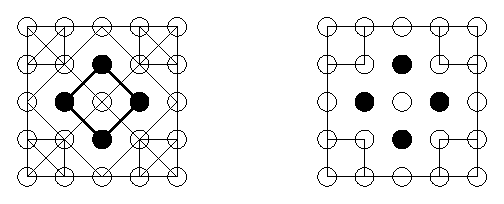
\includegraphics[width=8cm]{topoerreur}
  \caption[Paradoxe de connexit� pour un maillage par carr�]
  {Paradoxe de connexit� pour un maillage par carr�s, les
    ar�tes de ces graphes repr�sentent les diff�rentes connexit�s
    choisies (voir texte).}
  \label{fig:topoerreur}
\end{center}
\end{figure}

Une fa{\c c}on simple pour r�soudre le  paradoxe en 2D pour une grille
carr�e est de consid�rer une certaine connexit� pour  la courbe et une
autre pour son compl�mentaire. Ainsi, nous pouvons d�finir un analogue
discret du th�or�me de Jordan. 

\begin{theo}[S�parabilit� de \aut{rosenfeld}]
  Dans $\Z^2$, nous avons :
\begin{itemize}
\item le compl�mentaire de tout $4-$arc  (resp. un $8-$arc) est
  $8-$connexe (resp. $4-$connexe)~;
\item le compl�mentaire de toute $4-$courbe 
  (resp. une $8-$courbe)  a deux composantes
  $8-$connexes (resp. $4-$connexes) dont l'une est born�e et l'autre non.
\end{itemize}
\end{theo}



La garantie d'un certain  nombre  de propri�t�s topologiques sur   les
objets discrets est indispensable pour deux raisons principales, d'une
part les objets manipul�s  sont plus formalis�s et mieux contr{\^o}l�s,
mais aussi cela  permet  l'�criture d'algorithmes tr�s  efficaces pour,
par exemple, le parcours des   �l�ments d'une courbe discr�te ou  d'une
surface discr�te.   Il est donc n�cessaire de   choisir un cadre
topologique nous permettant de r�soudre ces probl�mes.


Pour cela, deux grandes approches  sont possibles, la premi�re appel�e
{\it topologie digitale} ({\it digital  topology} en anglais) consid�re  des
bords ou  des surfaces discr�tes comme  �tant  des ensembles de points
discrets (pixel ou voxels en 2D et 3D pour des pavage par hypercubes). La
seconde se   base  sur  une  d�composition  en �l�ments   de  dimension
inf�rieure appel�e {\it complexe cellulaire}.

\subsubsection{Approche bas�e sur les points discrets}
\label{sec:bord}
Dans cette approche,  la surface ou le contour  d'un objet discret est
un ensemble connexe de point discrets. On parle alors de {\it bord} ou
de  {\it  fronti�re}   ({\it   boundary} en  anglais).   Une  premi�re
d�finition constructive propos�e  par  \citet{morgenthaler} permet  de
caract�riser localement une  telle   surface dans le cas   d'un espace
discret dans $\Z^3$. L'id�e principale est  de v�rifi�e qu'il y a bien
s�paration locale dans un $26-$voisinage entre le bord et le
compl�mentaire. Cette caract�risation locale
permet cependant  d'�noncer un th�or�me  global de Jordan pour ce type
de surface.

Une d�finition de surface multidimensionelle et un algorithme de
parcours ont �t� propos� par \citet{udupa_boundary} et reposent sur une id�e
 simple : un point discret appartient au bord de l'objet s'il
poss�de un voisin dans le compl�mentaire (au sens de l'adjacence
attribu�e {\`a} celui-ci). 
%Ce type de surface est param�tr� par une paire
%de Jordan.

Une   autre   d�finition  de ce   type   de  surface  bas�e   sur  des
caract�risations        locales      a      �t�        propos�     par
\citet{BerMal96,Malgouyres:1997:DSZ}.  Dans ce  cadre-l{\`a}, une  version
discr�te du th�or�me de Jordan peut {\^e}tre prouv�e.

Un probl�me li�  {\`a}   ce  type de   surface  a �t�  illustr�    par
\citet{perroton}  et est pr�sent� dans  la figure \ref{fig:bord}. Tout
d'abord,  le bord  de l'objet  et le  bord  de  son compl�mentaire  ne
co{\"\i}ncident   pas.  De  plus,  une  autre  propri�t�  classique de
topologie   n'est pas   v�rifi�e   :   dans l'exemple   de   la figure
\ref{fig:bord}, le pixel du bord indiqu� par une fl�che est voisin des
deux composantes connexes de son compl�mentaire,  et les deux surfaces
que l'on   souhaiterait  (l'une  bornant  la   cavit�   et l'autre  le
compl�mentaire non-born�) se trouvent fusionn�es.


\begin{figure}[htbp]
\begin{center}
  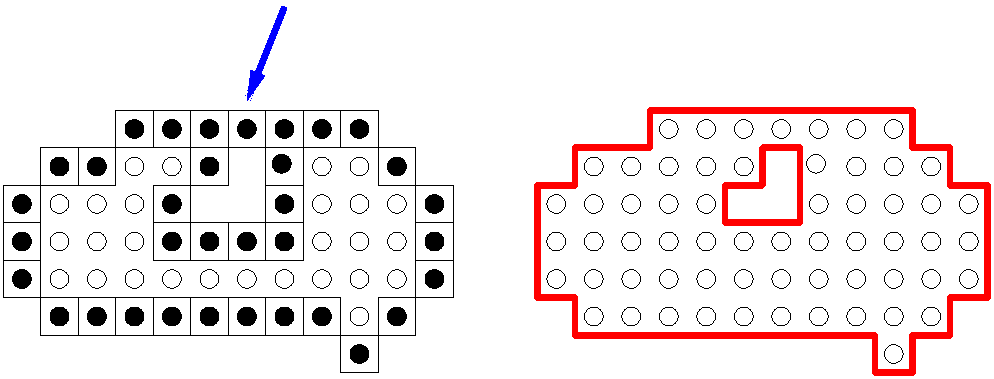
\includegraphics[width=12cm]{bord}
  \caption[D�faut de la notion de bord en tant qu'ensemble de points
    discrets]{D�faut de la notion de bord en tant qu'ensemble de points
    discrets (points noirs � gauche) et surface de lignels bas�e sur une
    approche cellulaire (polygones en gras � droite).}
  \label{fig:bord}
\end{center}
\end{figure}

\subsubsection{Approche bas�e sur les �l�ments de surface}
\label{sec:approche-surfel}

Dans  cette  approche,   des  �l�ments  (appel�s  {\it cellules})   de
dimension  inf�rieure    au  polygone  pavant   l'espace  discret sont
consid�r�s  (voir figure  \ref{fig:cellules}). Ainsi,  les cellules de
dimension 0 sont les {\it pointels}, les  �l�ments de dimension 1 sont
appel�s {\it lignels}, les faces ou �l�ments de dimension 2 sont
appel� {\it surfels}. Cette d�composition ainsi que la th�orie
topologique associ�e correspond � un cas particulier de complexe
simplicial baptis� {\it complexe cellulaire} pour des grilles dans
$\Z^n$ \citep{kovalevsky_arc}.

En se basant sur ce sch�ma de d�composition, \citet{artzy} et \citet{udupa}
ont propos� une d�finition de surface discr�te dans $\Z^n$ comme �tant un ensemble
connexe (au sens d'une certaine relation d'adjacence) de cellules de
dimension $n-1$ ``partageant'' un point discret de l'objet et un point
discret de son compl�mentaire. Par exemple en dimension 3, la surface discr�te est
un ensemble de {\it surfels} et ne sont consid�r�s que les surfels
partageant un voxel de l'objet et un voxel du fond.
\aut{Udupa} \etal consid�rent donc une $\kappa\lambda-$surface
discr�te d�finie par la paire de connexit�s dite de Jordan
$(\kappa,\lambda)$. Cette paire de connexit�s est une  extension 3D
de celle utilis�e dans le th�or�me de s�parabilit� de
\aut{Rosenfeld}. Ainsi, une surface d�finie par une paire
$(\kappa,\lambda)$ consid�re un objet $\kappa$-connexe et un fond
$\lambda$-connexe. Dans le cas 2D, les paires  $(4,8)$ et $(8,4)$ sont
dites de Jordan. En 3D nous avons les paires $(6,18)$, $(18,6)$,
$(6,26)$ et $(26,6)$.

La   relation        d'adjacence      entre   les    �l�ments       de
surfaces\footnote{relation  $\beta$ dans  \citet{udupa}} composant  la
$\kappa\lambda-$surface   permet   de    construire   des  algorithmes
d'extraction tr�s  efficaces  de   surfaces  discr�tes  en   dimension
quelconque (voir \citealt{perroton} par exemple pour le cas 3D).


Dans une approche purement complexe cellulaire, \citet{koval99} a
propos� une d�finition et un algorithme de parcours de surfaces discr�tes.


\begin{figure}[htbp]
\begin{center}
  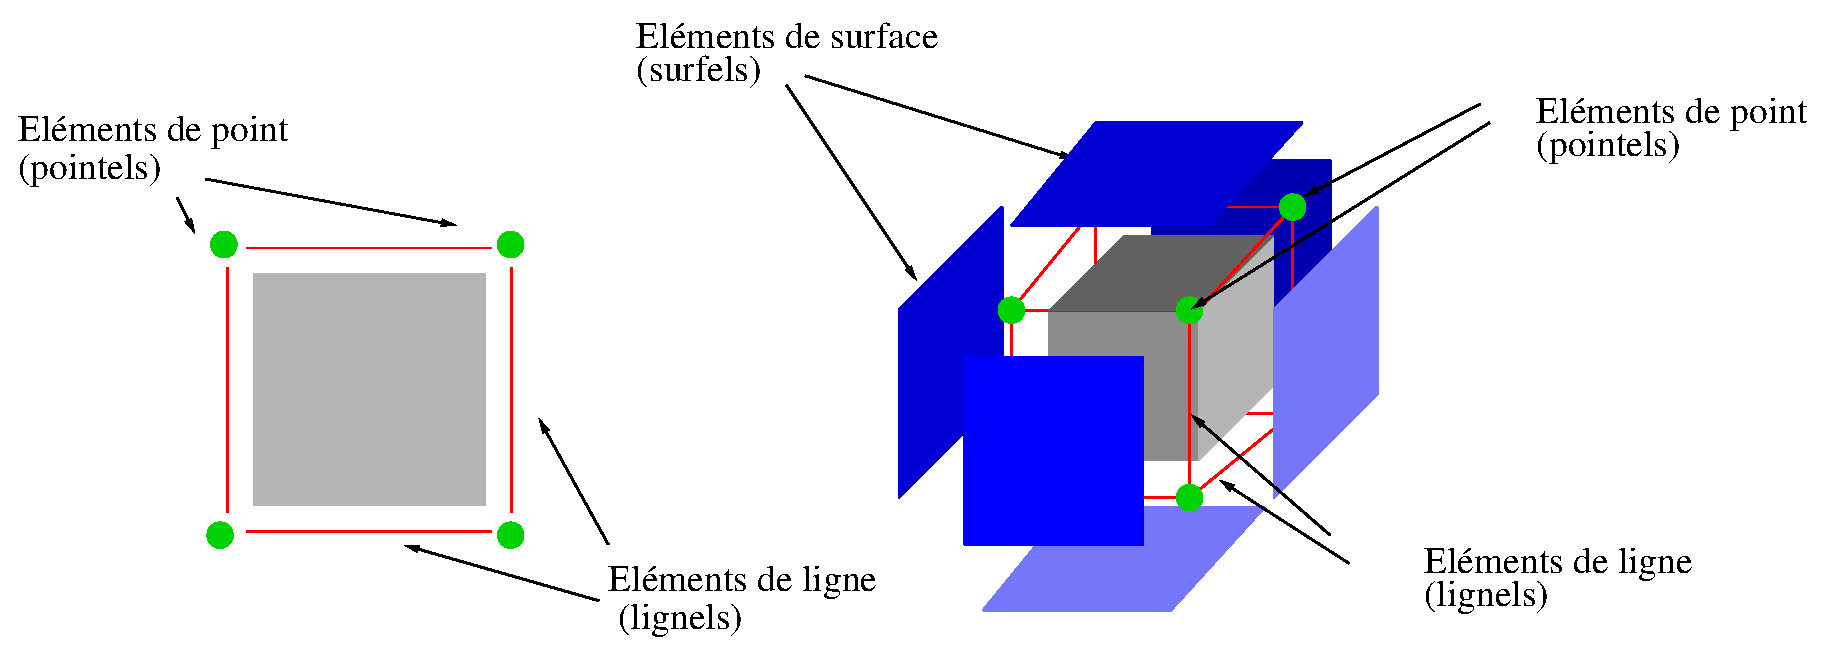
\includegraphics[width=12cm]{elements}
  \caption{D�composition d'un pixel et d'un voxel en cellules
    de dimensions inf�rieures.}
  \label{fig:cellules}
\end{center}
\end{figure}


\section{Codage et propri�t�s du codage des courbes discr�tes}

Dans    cette partie, nous   introduisons les  codages  usuels pour la
repr�sentation de  courbes dans un espace  discret. L'objectif est ici
de proposer un codage de la courbe discr�te ayant les propri�t�s de~:
\begin{description}
\item[compacit�] : compression du codage par rapport � une liste de
  coordonn�es des points discrets
\item[r�versibilit�] : possibilit� de reconstruire la courbe � partir du
  codage
\item[invariance] : dans quelle mesure le code est-il invariant par
  certaines transformations g�om�triques ?
\item[informative] : Est-il possible d'extraire des informations au
  sens large sur la courbe � partir du codage (par exemple sa
  longueur\ldots) ?
\end{description}


Un   codage  usuel       d'une   courbe  discr�te      est   celui  de
\citet{Fre-encoding-agc} qui consiste � introduire $k$ labels pour les
connexit�s possibles d'une $k-$courbe (voir \ref{fig:freeman} pour les
codes 2D). Ensuite le codage consiste � associer le code qui correspond
� chaque d�placement en $k-$connexit� dans la courbe discr�te. 
Il suffit donc de m�moriser les coordonn�es du point de d�part et le code de chaque d�placement pour reconstruire la courbe. 

\begin{figure}[htbp]
\begin{center}
  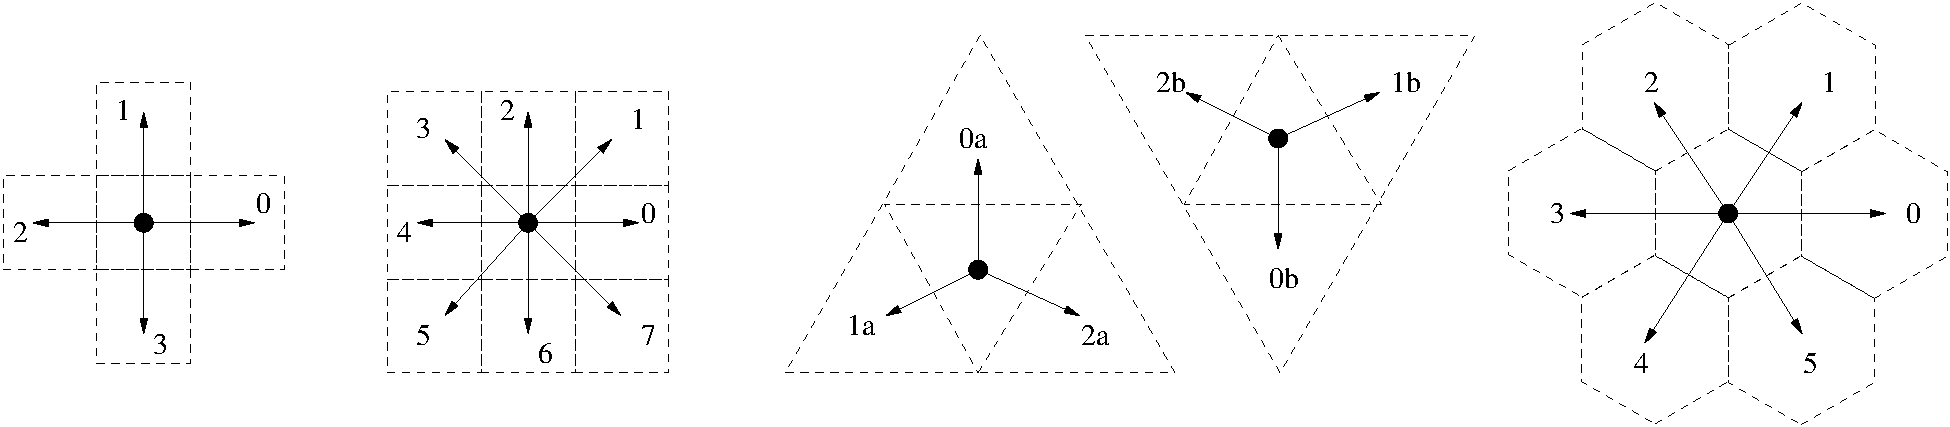
\includegraphics[width=14cm]{freeman}
  \caption[Codage de \aut{freeman}]{Codage de \aut{freeman} pour la $4-$ et la $8-$connexit� du
    pavage par carr�, les codages pour les $3-$connexit� pour le
    pavage triangulaire et la $6-$connexit� pour la grille hexagonale.}
  \label{fig:freeman}
\end{center}
\end{figure}


\begin{figure}[htbp]
\begin{center}
  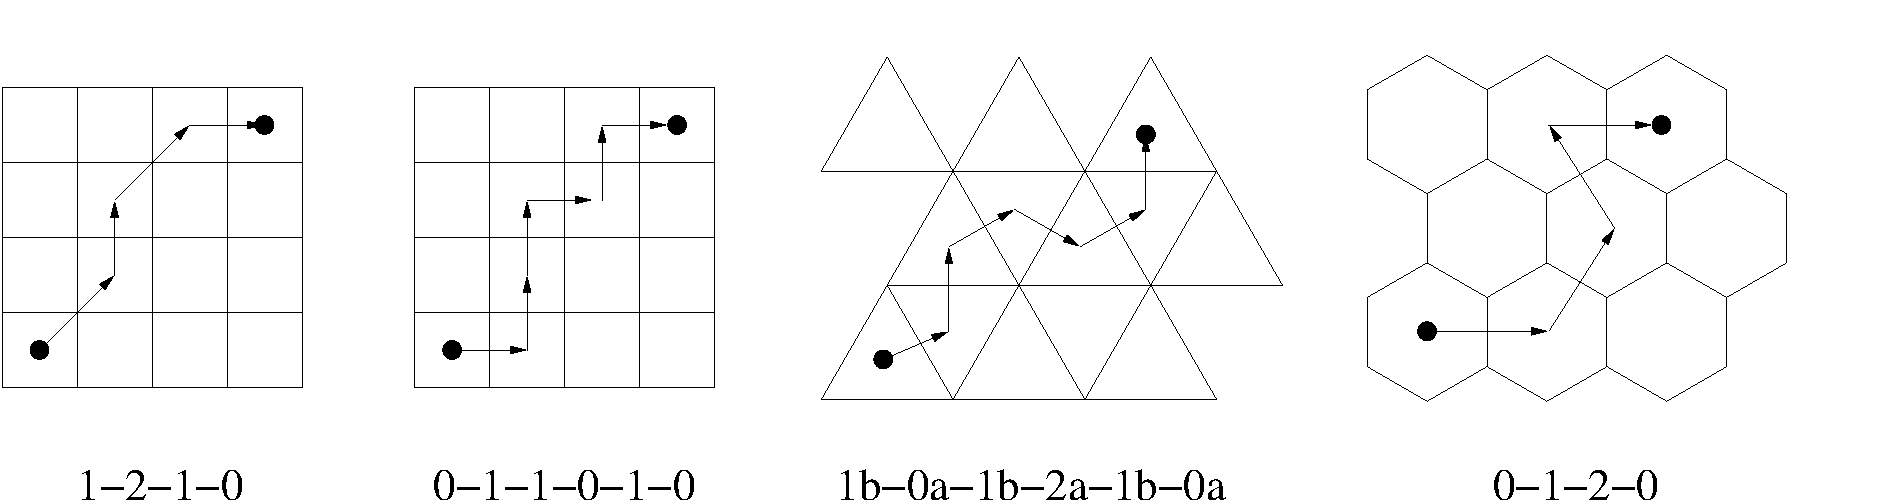
\includegraphics[width=14cm]{codage_freeman}
  \caption[Codage de \aut{freeman} d'arcs]{Codage de \aut{freeman}
    d'arcs respectivement $8-$connexe, $4-$connexe, $3-$connexe et
    $6-$connexe en utilisant les codes de    la figure \ref{fig:freeman}.}
  \label{fig:codage}
\end{center}
\end{figure}

Ce codage de \aut{freeman} a de nombreuses propri�t�s \citep{montanvert} :
il permet notamment de segmenter une courbe discr�te en quadrants,
octants, sextants \ldots en fonction de l'espace discret. On peut aussi
voir des transformations simples telles que la translation, la sym�trie
d'axes, la rotation, comme des processus de r��criture sur le code. Par
exemple, pour une rotation de $\pi/2$ dans le sens trigonom�trique d'une
courbe $8-$connexe, il suffit de remplacer le code
$(\{c_i\},(x,y))$ tel que les $c_i$ sont les �l�ments du code et
  $(x,y)$ sont les coordonn�es du point de d�part, par~:

\begin{displaymath}
\left \{  \begin{array}{l}
  c'_i = c_i + 2\quad mod (8) \\
  (x',y')= (y,x)
  \end{array} \right.
\end{displaymath}

Dans un objectif de comparaison de courbes discr�tes par leur code,
le codage de \aut{freeman} souffre du probl�me de variance par sym�trie
d'axe.

D'autres codes existent, ceux-ci diff�rent de l'application que l'on en
fait. Nous pr�sentons , par exemple, un codage tr�s simple qui est lui
invariant par sym�trie. \citet{Bri1999} propose un codage de chaque
{\it pointel} de la surface de l'objet par le nombre de points discrets de l'objet
auxquels ce pointel est adjacent (voir figure \ref{fig:brib}). Ce code
a les propri�t�s suivantes :
\begin{itemize}
\item invariance au choix du point de d�part~;
\item invariance par rotations d'angles $k\pi/2$ (avec $k\in\Z$)~;
\item invariance par sym�trie d'axe~;
\item permet le calcul de la longueur au sens de \aut{freeman}~;
\item permet le calcul du code du compl�mentaire par simple r��criture ~;
\item transposition possible entre ce code et le codage de~;
  \aut{freeman}, la propri�t� de synth�se est donc v�rifi�e~;
\item extraction des caract�ristiques d'\aut{Euler} � partir du code.

\end{itemize}

\begin{figure}[htbp]
\begin{center}
  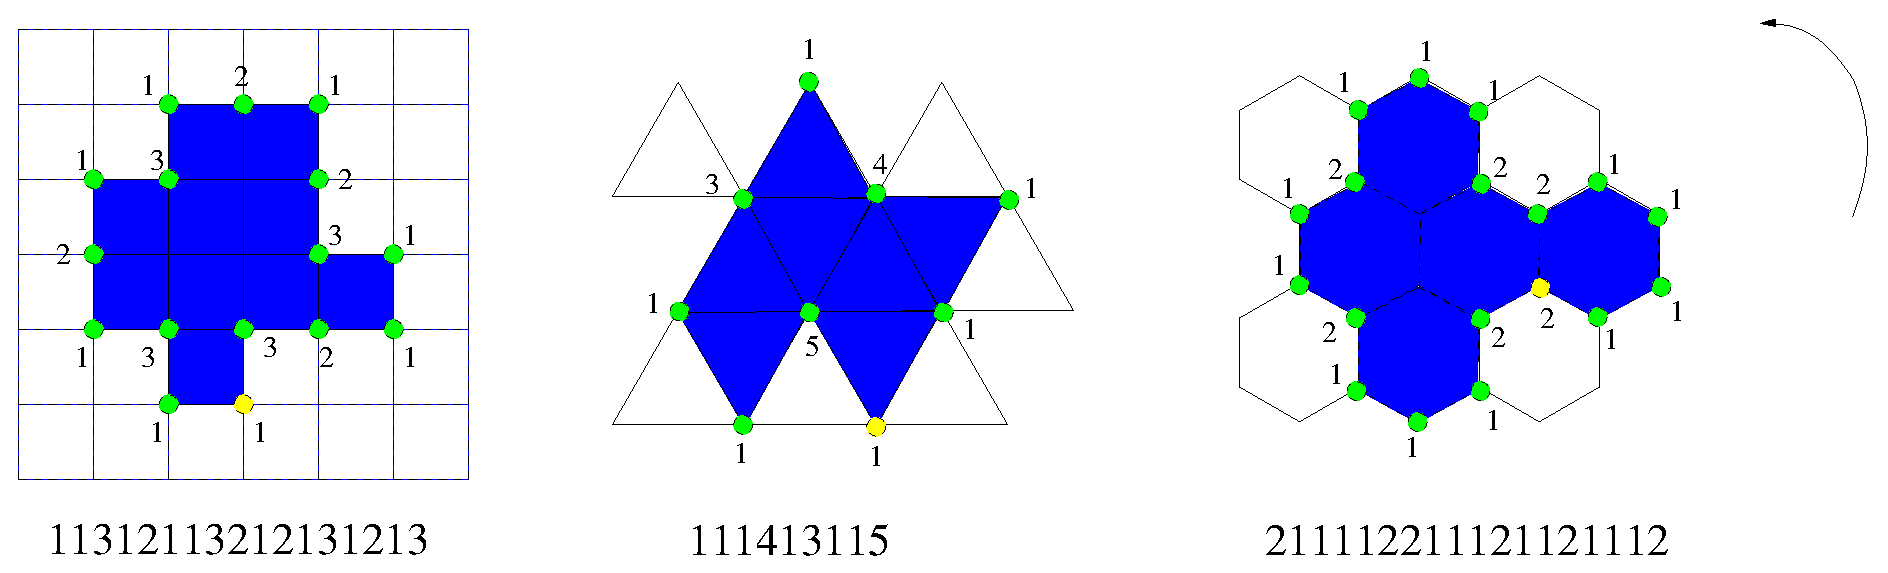
\includegraphics[width=14cm]{codage_bribiesca}
  \caption[Codage de \aut{Bribiesca}]{Codage de \aut{Bribiesca} pour la $4-$ et la $8-$connexit� du
    pavage par carr�, les codages pour les $3-$connexit� pour le
    pavage triangulaire et la $6-$connexit� pour la grille hexagonale.}
  \label{fig:brib}
\end{center}
\end{figure}


\section{Processus de discr�tisation}

Pour terminer cette introduction des notions de base en g�om�trie
discr�te utiles pour la suite, nous d�taillons les diff�rents processus de
discr�tisation que nous serons amen�s � utiliser.

Le contexte est le suivant : nous consid�rons un objet continu
$\mathcal{O}$ ou uniquement son bord, not� $\gamma$, et nous souhaitons
construire l'ensemble des points discrets qui sont les
{\it discr�tis�s} soit de $\mathcal{O}$, soit de $\gamma$.
Dans ce qui suit, nous nous int�ressons plus particuli�rement au
pavage par carr�s et donc � des grilles dans $\Z^n$.

\citet{jonas97} proposent un ensemble de propri�t�s permettant une
comparaison th�orique de ces processus de discr�tisation :

\begin{description}
\item[Permutation du syst�me d'axes] : est-ce que la discr�tisation
  du sym�trique par rapport � un axe de $\gamma$ est le sym�trique de
  la discr�tisation de $\gamma$ ?
\item[Invariant par translation enti�re] : le processus est-il d�pend
  d'une origine sur la grille ?
\item[Perturbation locale] : est-ce qu'une petite perturbation locale
  de $\gamma$ n'entra�ne qu'une perturbation locale sur la
  discr�tisation ?
\item[Droite-arc] : est-ce que la discr�tisation d'une droite est un
  $k-$arc (pour une relation d'adjacence donn�e) ?
\item[Propri�t� de projection] : pour les dimensions sup�rieures,
  est-ce le discr�tis� du projet� sur un hyper-plan canonique de la
  grille co�ncide avec le projet� du discr�tis� ?
\item[Convergence en distance] : est-ce que la discr�tisation converge
  selon une certaine m�trique vers la courbe ou l'objet continu pour
  une r�solution de grille croissante ?
\end{description}

\subsection{Discr�tisations classiques}

Dans un  premier temps, nous  consid�rons  que  la courbe $\gamma$  en
position g�n�rale.  C'est-�-dire qu'elle  a une  probabilit� nulle de
passer par  un sommet du pavage de  l'espace discret et de  croiser une
ar�te du maillage � �gale distance des deux sommets adjacents �
 celle-ci. Nous verrons par la suite des processus de discr�tisation qui g�rent ces cas pathologiques. 


Un premier processus de discr�tisation a pour analogie le trac� de
droite de \citet{bres65} : lorsque l'on a le choix entre deux points
discrets, c'est-�-dire � chaque fois que la courbe $\gamma$ croise
une ar�te du maillage discret, on choisit celui qui est le plus
proche. Ce processus s'appelle {\it Grid Intersect Quantization} (ou
GIQ) et est illustr� sur le premier sch�ma de la figure
\ref{fig:disc}.

S'il on consid�re maintenant la discr�tisation d'un objet et non d'une
courbe, nous pouvons d�finir les discr�tisations {\it interne} et {\it
  externe} de l'objet. Dans ce cas, lors du choix entre deux points
discrets, nous choisissons respectivement celui qui est dans l'objet
ou celui qui est ext�rieur � celui-ci (voir figure
\ref{fig:disc}). Ces discr�tisations sont appel�es respectivement {\it
  Object Boundary Quantization} (OBQ) et {\it  Background Boundary
  Quantization} (BBQ).

\begin{figure}[htbp]
\begin{center}
  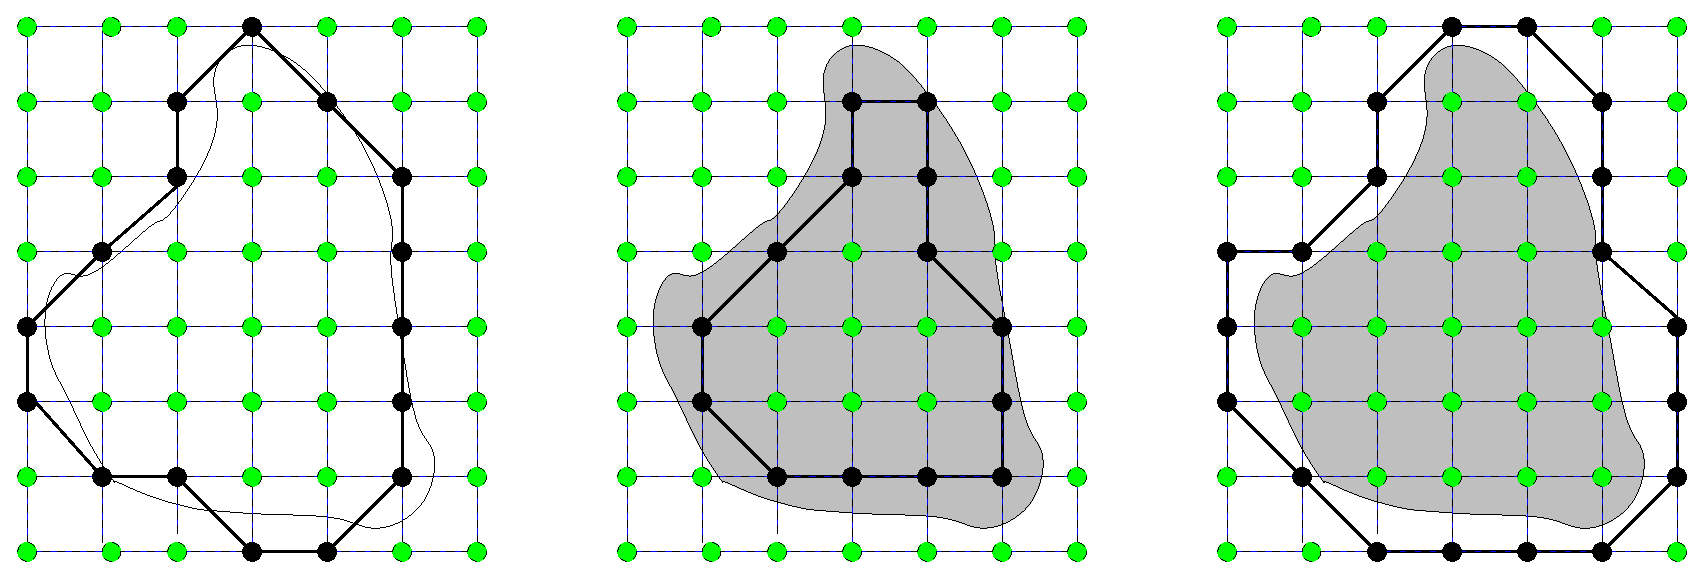
\includegraphics[width=14cm]{discretisations}
  \caption[ Processus de discr�tisation classiques]{Processus de discr�tisation classiques : ({\it de gauche �
droite}) {\it Grid Intersect Quantization}, {\it Object Boundary
Quantization} et {\it Background Boundary Quantization}.}
  \label{fig:disc}
\end{center}
\end{figure}

Ces discr�tisations simples peuvent �tre facilement �tendues pour des
grilles dans $\Z^n$ (voir \citealt{jonas97} par exemple pour la 3D).


\subsection{Discr�tisation de simplexes}
\label{sec:discr-de-simpl}

Dans    ce  paragraphe, on   s'int�resse   au  cas  particulier  de la
discr�tisation de  points,  de droites, de  plans  ou d'hyper-plans en
dimension $n$~; ou encore de  $m$-simplexes (facettes de dimension $m$
dans un espace  de  dimension  $n$).  Pour  ce type  d'objet,  les cas
pathologiques  ne peuvent pas �tre  supprim�s et  doivent �tre pris en
compte.

De plus, certains de  ces  mod�les  permettent d'avoir des   �critures
analytiques des discr�tisations des  objets. C'est le cas notamment de
la  notion  de  {\it supercouverture}  (voir  \citealt{montanvert} par
exemple)   dont la description  analytique   pour des $m-$simplexes en
dimension  $n$     a    �t�   propos�e   par    \aut{andr�s}     (voir
\citealt{andres_hdr}  par  exemple).      Dans ce  mod�le,     les cas
pathologiques d�crits pr�c�demment  s'appellent des  {\it bulles} (voir figure
\ref{fig:discbis}).

\cite{andres_standard} a aussi r�cemment propos� un autre mod�le,
appel� {\it standard}, permettant aussi une �criture analytique des
objets discr�tis�s et ne contenant plus de {\it bulles} par le biais
de convention d'orientations dans $\Z^n$.

Dans une approche plus topologique, \citet{couprie_discretization} ont
propos� un mod�le proche du mod�le de supercouverture mais bas� sur
une approche complexe cellulaire. Dans ce cas, la notion de {\it
  bulles} comme �tant des {\it singularit�s} du mod�le
dispara�t. Cependant, ce mod�le n'est disponible qu'en dimensions 2 et 3 et n'est
pas encore g�n�ralis�.

\begin{figure}[htbp]
\begin{center}
  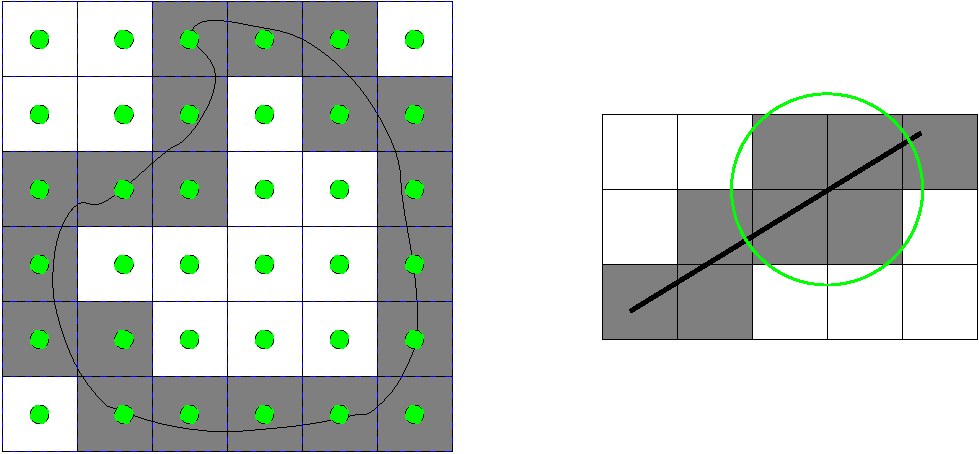
\includegraphics[width=10cm]{discretisationsbis}
  \caption[Discr�tisation par  supercourvertures]{Discr�tisation par  supercourvertures : ({\it gauche})
    discr�tisation d'une courbe quelconque et illustration d'une {\it
      bulle} pour la discr�tisation d'une droite.}
  \label{fig:discbis}
\end{center}
\end{figure}



\section{Conclusion}

Dans ce chaptire nous avons pr�sent� quelques  notions
de base en g�om�trie discr�te. Nous avons d�fini la notion d'espace
discret, de point discret et d'objets simples sur cet espace (objet, courbe
surface). Nous avons aussi pr�sent� les diff�rents codages des courbes
dans le cas 2D. Nous avons termin� ce chapitre par une description des
principales discr�tisations d'objets euclidiens  qui nous serviront par la
suite.




%%% Local Variables: 
%%% mode: latex
%%% TeX-master: "these"
%%% End: 
% LocalWords:  pixel

%
%%%%%%%%%%%%%%%%%%%%%%%%%%%%%%%%%%%
\mychaptoc{Droites et Plans discrets}\label{chap-droites}
%%%%%%%%%%%%%%%%%%%%%%%%%%%%%%%%%%


\section{Introduction}

Dans ce  chapitre nous nous int�ressons  aux objets fondamentaux de la
g�om�trie  discr�te que sont les droites  et les  plans discrets.  Ces
objets de base permettent l'�laboration,  sur le plan th�orique, d'une
g�om�trie discr�te.

Dans  les deux premiers  paragraphes,  nous analysons les  diff�rentes
d�finitions et algorithmes associ�s  aux droites discr�tes dans $\Z^2$
et dans $\Z^3$.  Nous reprenons les diff�rentes �tudes pr�sent�es dans
la   litt�rature   pour   lesquelles nous   proposons  une  �valuation
comparative.

Dans  le  paragraphe   \ref{sec:plans-discrets},  nous   effectuons un
travail  similaire   sur les plans  discrets   en proposant un premier
th�or�me de structure de la {\it pr�-image} d'un plan discret.

Enfin,   dans   le   paragraphe   \ref{sec:statistique-pour-la},  nous
pr�sentons  une   alternative   � l'approche    g�om�trique pour    la
reconnaissance de droites et plans  discrets. Cette nouvelle  approche
se base sur une analyse statistique de ces objets.


%%%%%%%%%%%%%%%%%%%%%%%%%%%%%%%%%%%%%%%%%%%%%%%%%%%%%%%%%%%%%%%
\section{Droites discr{\`e}tes 2D}
\label{sec:droites-discretes-2d}

Nous commen�ons notre analyse des objets discrets par la notion de
droite discr�te.  Les d�finitions, propri�t�s et algorithmes associ�s
� ces objets sont primordiaux dans de nombreux domaines, par exemple
en analyse d'image  ou en reconnaissance de formes. 

La notion de droite discr�te est importante, non seulement sur le plan
th�orique comme objet de base du mod�le  discret, mais aussi cet objet
et les algorithmes qui lui sont associ�s sont  des outils de base pour
des estimations   de    mesures   euclidiennes    sur   des     objets
discrets. Ainsi, une  bonne ma�trise de  cette {\it brique de base} de
la g�om�trie discr�te est  n�cessaire avant de voir  ses applications
dans la  caract�risation de formes  des chapitres \ref{chap-metriques}
et \ref{chap-mesuresa}.

\subsection{D�finitions et propri�t�s}
\label{sec:defin-et-propr}

Sur la grille discr�te, de nombreuses approches existent pour d�cider
si un ensemble de pixels  a une allure {\it rectiligne}. Bien
�videmment, nous devons tout d'abord d�finir un peu plus formellement
la notion de lin�arit� pour un ensemble de points discrets.
Dans ce qui suit, nous utilisons les notions de {\it quadrant} ou {\it
  d'octant} pour un segment de droite en fonction d'une partition de
l'espace 2D en 4 ou 8 r�gions (voir figure \ref{fig:octants}).

\begin{figure}[htbp]
   \begin{center}
    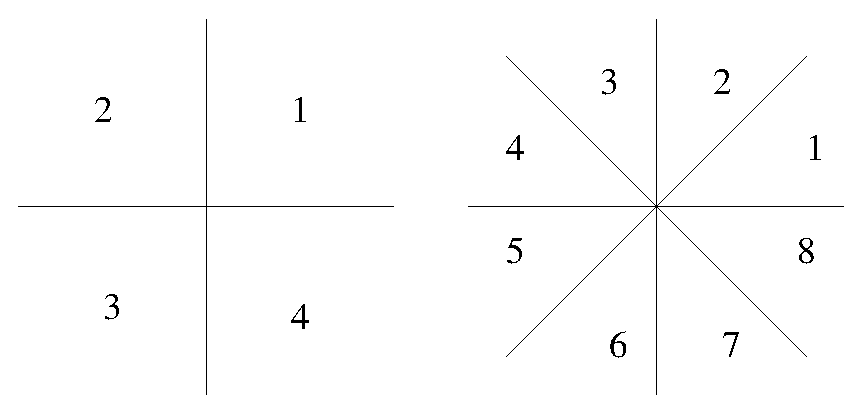
\includegraphics[width=6cm]{octants}
    \caption{D�composition de l'espace 2D en quadrants $(gauche)$ et
      en octants $(droite)$.}
    \label{fig:octants}
  \end{center}
\end{figure}



D'une mani�re g�n�rale, un ensemble  de points de la grille appartient
� une  {\it  droite discr�te} s'il existe  une  droite  r�elle dont la
discr�tisation contient les pixels  consid�r�s.  Par exemple, si  nous
consid�rons le processus  de discr�tisation OBQ ({\it Object  Boundary
Quantization}),  un ensemble de  pixels  $\mathcal{E}$ appartient � une
droite discr�te s'il existe   au moins un couple $(\alpha,\beta)$   de
$\R^2$ tel que tous les points $(x,y)$ de $\mathcal{E}$ v�rifient~:

\begin{displaymath}
  0\leq \alpha x+\beta-y <1
\end{displaymath}



Sur  le  plan  m�thodologique,  certaines  approches   partent   de ce
processus de discr�tisation  pour �noncer  les propri�t�s des  droites
discr�tes qu'elles proposent~; d'autres ne travaillent qu'au niveau de
la  grille, elles �noncent  les propri�t�s et  ensuite montrent qu'une
droite r�elle discr�tis�e v�rifie celles-ci.

Avant d'�noncer les constructions classiques de  ces objets, la figure
\ref{fig:vialard_droites}  illustre les  subtilit�s,  au  moins sur le
plan visuel, pour qu'un  arc discret soit,  ou non, un segment discret
(figure tir�e  de \citealt{vialardthese}).   Dans   ce cas, la  figure
$(a)$ est  un morceau  de droite  discr�te, $(b)$  n'en est pas  un et
$(c)$ non plus.


\begin{figure}[htbp]
  \begin{center}
    \subfigure[]{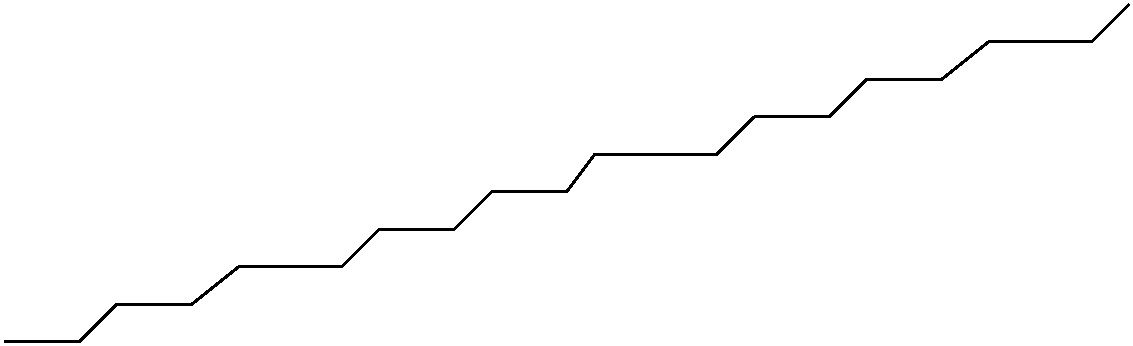
\includegraphics[width=4cm]{vialard_droites1}}
    \subfigure[]{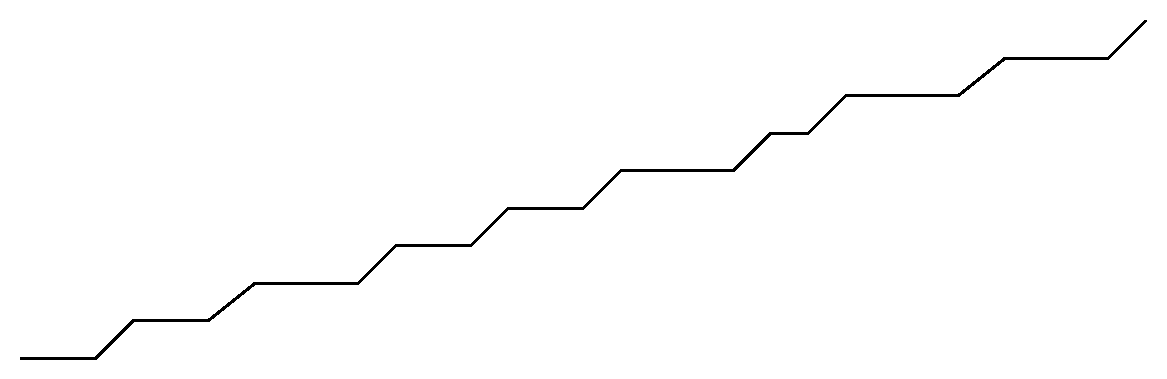
\includegraphics[width=4cm]{vialard_droites2}}
    \subfigure[]{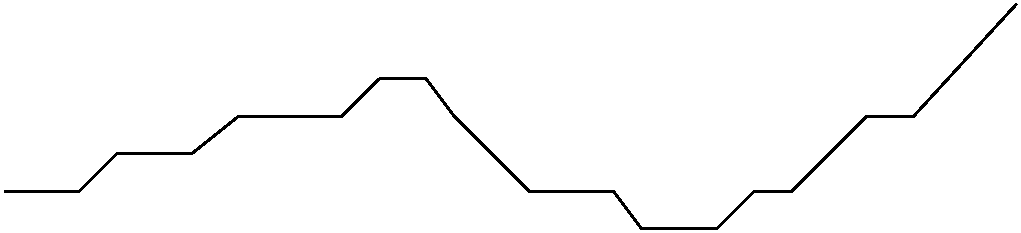
\includegraphics[width=4cm]{vialard_droite3}}
    \caption{Seul l'arc $(a)$ est un segment discret selon
      les d�finitions usuelles des droites discr�tes (cf ci-dessous).}
  \label{fig:vialard_droites}
\end{center}
\end{figure}

\subsubsection{Caract�risation}


Consid�rons tout  d'abord le cas d'un arc   discret 8-connexe. Une des
premi�res  caract�risations des  droites discr�tes a   �t� propos�e par
\citet{Freeman:1974:CPL} et est bas�e  sur le codage de l'arc.  Ainsi,
un arc est un segment discret si~:

\begin{itemize}
\item son codage ne contient que deux codes diff�rents et ceux-ci ne
  diff�rent que de 1 (modulo 8)~;
\item un de ces deux codes est toujours isol� dans le codage~;
\item ce code isol� appara�t dans le codage le plus uniform�ment possible.
\end{itemize}
Dans cette caract�risation, la derni�re propri�t� est assez floue et
cette d�finition globale d'un segment discret n'est pas encore
satisfaisante.

\begin{figure}[htbp]
  \begin{center}
    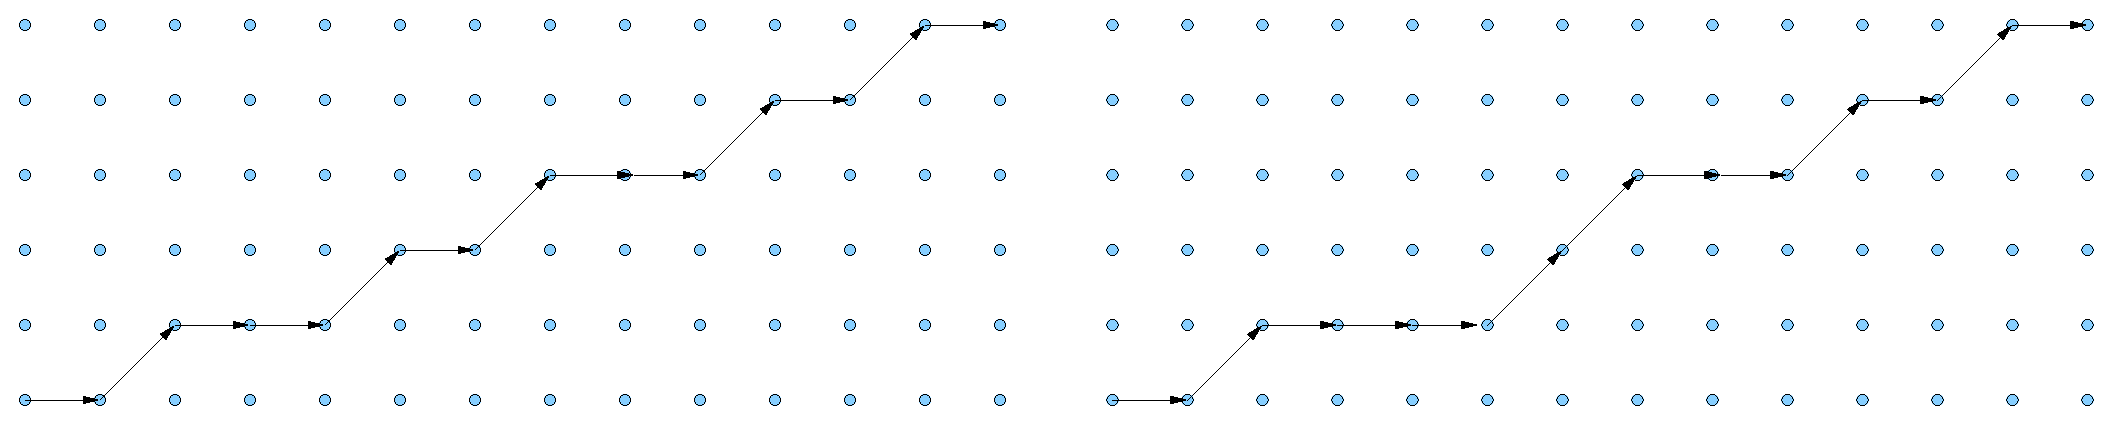
\includegraphics[width=12cm]{Fig/freeman_prop}
    \caption[Propri�t�s de \aut{freeman}]{Propri�t� de \aut{freeman}~:
      {\it  (gauche)} le codage est $0-1-0-0-1-0-1-0-0-1-0-1-0$, les
      codes ``1'' apparaissent isol�s et {\it uniform�ment} r�partis~; {\it
        (droite)}, le codage est $0-1-0-0-0-1-1-0-0-1-0-1-0$, dans ce
      cas, ni le code ``0'' ni le code ``1'' sont isol�s, cet arc
      n'est pas un segment discret.}
    \label{fig:freeman_prop}
  \end{center}
\end{figure}



Par la suite, \cite{rosenfeld} introduit une propri�t� importante
permettant de caract�riser un segment discret~: {\it la propri�t� de la
  corde}. Tout ensemble de points discrets qui v�rifie cette propri�t�
est un morceau de droite discr�te et r�ciproquement, tous les points
d'un segment discret v�rifient celle-ci.

Cette propri�t� s'�nonce de la fa�on suivante (voir figure \ref{fig:corde})~:

\begin{defi}[Propri�t� de corde]
\label{defi:corde}    Un ensemble de pixels $\mathcal{E}$ v�rifie la propri�t� de corde
    si pour tout couple $p$ et $q$ de $\mathcal{E}$, et pour tout
    point $m(x,y)$ du segment $[pq]$, il existe un point $M(i,j)$ de
    $\mathcal{E}$ tel que
    \begin{displaymath}
      max(|i-x|,|j-y|)<1
    \end{displaymath}
\end{defi}

\begin{figure}[!h]
  \begin{center}
    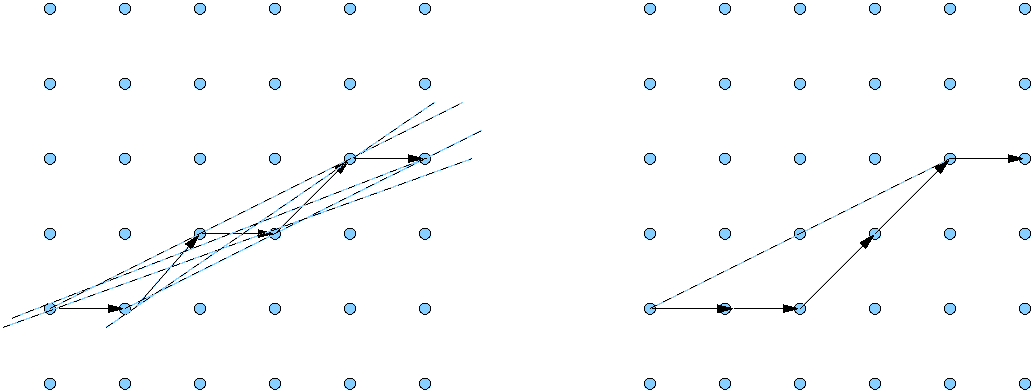
\includegraphics[width=10cm]{Fig/corde_prop}
    \caption[Propri�t� de corde de \aut{Rosenfeld}]{Propri�t� de corde
      de \aut{Rosenfeld}~: {\it  (gauche)} tous les segments $[pq]$ de
      longueur sup�rieure � 2  v�rifient cette propri�t�, cet arc est
      donc un segment discret~; {\it (droite)}, existence d'un
contre-exemple, ce segment ne correspond donc pas � un morceau de
      droite discr�te.} 
    \label{fig:corde}
  \end{center}
\end{figure}


Cette  propri�t� permet une  caract�risation  formelle des segments de
droites discr�tes mais n'est pas constructive  dans le sens o� elle ne
permet  pas directement  de tracer  ou de  reconna�tre  un tel segment
autrement que par un test exhaustif.

En se basant  sur   une    r��criture  des crit�res    de   \aut{Freeman} par
\citet{HUE_1981}, \citet{wu}   prouve  l'�quivalence entre  ces crit�res  et   la
propri�t� de corde de \citeauthor{rosenfeld}.


Dans une approche similaire � la propri�t� de corde, \cite{Hung85} propose une
caract�risation des droites discr�tes bas�e sur la notion  {\it
  d'uniformit�} ou de {\it r�gularit�} (traduction de {\it evenness},
voir figure \ref{fig:evenness}).

\begin{defi}[Propri�t� de r�gularit�]
  Un ensemble de pixels $\mathcal{E}$ dans le premier octant est dit r�gulier
  si tout quadruplet  de points $(a,b,c,d)$ de $\mathcal{E}$, tel
  que $\vec{ba}_x=\vec{dc}_x$, v�rifie~:
  \begin{displaymath}
    |\vec{ba}_y-\vec{dc}_y|=1
  \end{displaymath}
\end{defi}

\begin{figure}[!h]
  \begin{center}
    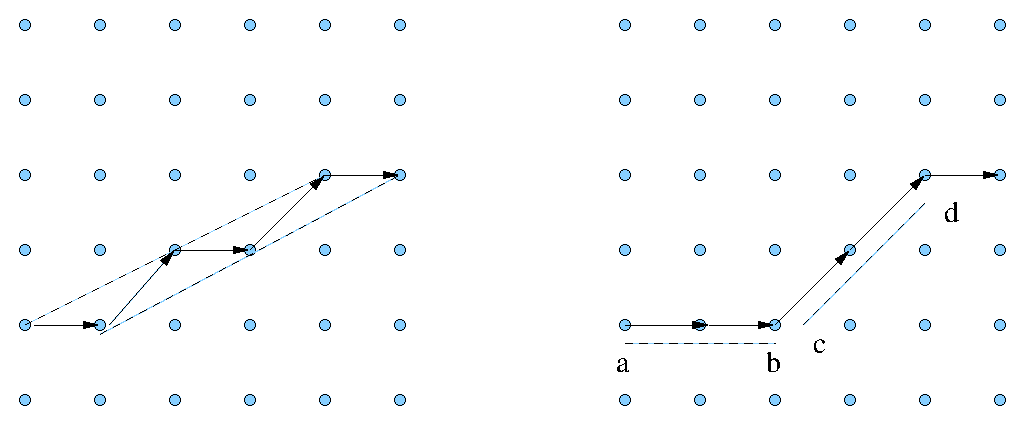
\includegraphics[width=10cm]{Fig/evenness_prop}
    \caption[Propri�t� de r�gularit� de \citeauthor{Hung85}]{Propri�t� de
      r�gularit� de \citeauthor{Hung85}~: {\it  (gauche)} tout quadruplet
      $(a,b,c,d)$ v�rifie la propri�t� de r�gularit�, cet arc est
      donc un segment discret~; {\it (droite)}, existence d'un
contre-exemple, les vecteurs $\vec{ab}$ et $\vec{cd}$ ne v�rifient pas
      cette propri�t�, ce segment ne correspond donc pas � un morceau de
      droite discr�te.}
    \label{fig:evenness}
  \end{center}
\end{figure}

 \citet{Smeulders84} proposent non seulement
une caract�risation des droites discr�tes, mais aussi un codage unique
des segments discrets. A partir d'un codage de \aut{Freeman} d'un
segment discret, ils introduisent un quadruplet d'entiers
$(n,q,p,s)$ d�crivant enti�rement ce segment discret. Consid�rons, sans
perte de g�n�ralit�s, un segment dans le premier octant. Le codage
de \aut{freeman} est donn� par les codes $\{c_i\}_{i=1...n}$, nous
avons alors (voir figure \ref{fig:dorst_quadurplet})~:


\begin{itemize}
\item $n$ repr�sente la longueur du segment de droite discr�te~;
\item $q$ la {\it p�riode} dans le code de \aut{freeman}. Ce param�tre
  s'�crit formellement~:
  \begin{displaymath}
    q=\min_{k}\{k \in \{1,2,\ldots,n\} \quad | \quad k=n \vee \forall i\in
    \{1,2,\ldots,n-k\} \quad c_{i+k}=c_i\} 
  \end{displaymath}

\item $p$ est la {\it hauteur} sur la p�riode, c'est-�-dire~:
  \begin{displaymath}
    p=\sum_1^q c_i
  \end{displaymath}
\item $s$ est le d�phasage du segment par rapport � la p�riode
  $q$. Nous avons formellement~:
  \begin{displaymath}
    s:~s\in\{0,1,\ldots,q-1\}\quad|\quad\forall i \in
    \{1,2,\ldots,q\}:\quad c_i=\left \lfloor \frac{p}{q}(i-s)\right \rfloor -
    \left \lfloor \frac{p}{q}(i-s-1)\right\rfloor
  \end{displaymath}
\end{itemize}

D'une mani�re informelle, le param�tre $q$ correspond � la r�gle {\it
  d'uniformit�} de \aut{freeman} (troisi�me crit�re).

A partir de ce codage $(n,q,p,s)$, une droite euclidienne telle que sa
discr�tisation avec OBQ correspond au segment discret est donn�e par~:
\begin{displaymath}
  y=\frac{p}{q}(x-s)+\left\lceil\frac{sp}{q}\right\rceil
\end{displaymath}
Cependant, l'ensemble des droites solutions se caract�rise enti�rement
avec ce quadruplet. Ainsi, \citet{Smeulders84} d�taillent la
construction de ce domaine des droites ou {\it pr�-image} dans
l'espace des param�tres $(\alpha,\beta)$ des pentes et des ordonn�es �
l'origine des droites.

\begin{figure}[!h]
  \begin{center}
    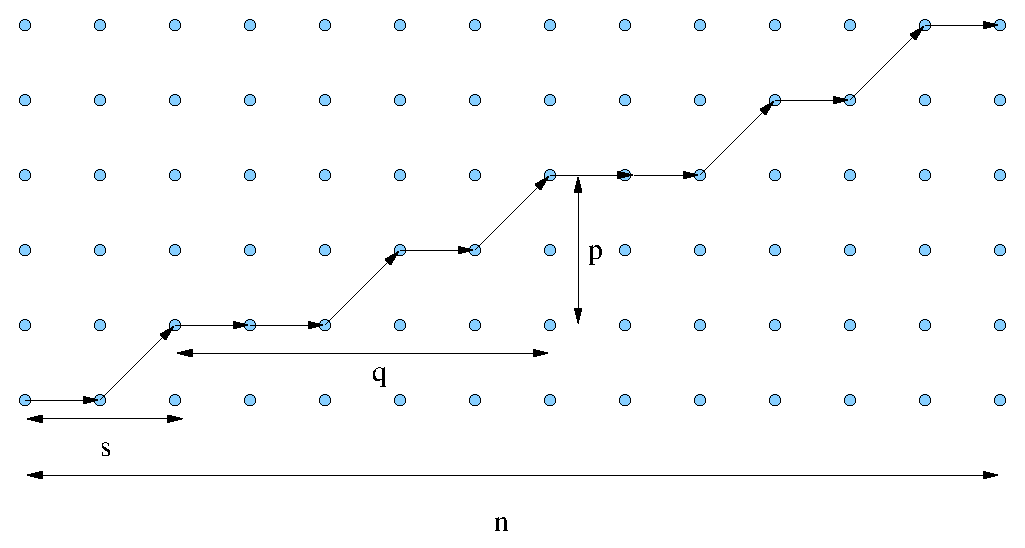
\includegraphics[width=10cm]{Fig/dorst_quadurplet}
    \caption{Repr�sentation graphique des quadruplets $(n,q,p,s)$ de
      \citeauthor{Smeulders84} pour la caract�risation des droites
      discr�tes~; notre segment se code donc $(14,5,2,2)$.}
    \label{fig:dorst_quadurplet}
  \end{center}
\end{figure}

Dans une m�me approche de construction du domaine des droites ou de la
{\it pr�-image} de l'arc discret, \citet{LindenbaumKoplowitz91}
proposent un autre codage bas� sur les s�ries de \aut{Farey} (voir
paragraphe \ref{sec:approche-dual}) et d�crivent un processus de conversion entre ce
codage et celui de \citeauthor{Smeulders84}. Nous reviendrons dans le
paragraphe suivant sur les diff�rentes techniques de reconnaissance de
droites discr�tes bas�es sur ce type de codage.


\subsubsection{Droites discr�tes arithm�tiques}

Nous pr�sentons une derni�re caract�risation que nous allons beaucoup
utiliser par la suite, celle propos�e par
\citet{reveilles}~:

\begin{defi}[Droite discr�te arithm�tique]
  Un  ensemble de pixels $\mathcal{E}$ appartient  � la droite discr�te
  arithm�tique de pente  $\frac{a}{b}$, de  borne inf�rieure $\mu$  et
  d'�paisseur $\omega$  (avec $a$, $b$, $\mu$   et $\omega$ dans $\Z$,
  $b\neq0$ et  $pgcd(a,b)=1$),  si  et  seulement si tous   les pixels
  $(x,y)$ de $\mathcal{E}$ v�rifient~:
  \begin{equation}
    \label{eq:droite_disc}
    \mu \leq ax-by<\mu+\omega
  \end{equation}
Cette droite se note $\mathcal{D}(a,b,\mu,\omega)$.
\end{defi}
\begin{figure}
  \begin{center}
    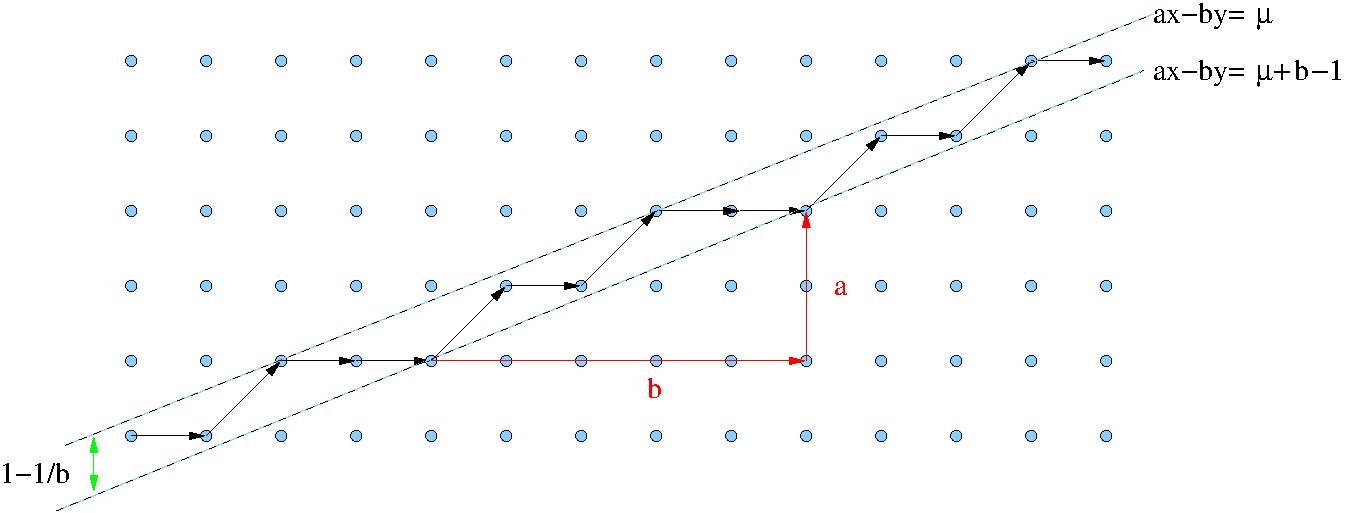
\includegraphics[width=12cm]{Fig/reveilles_prop}
    \caption{Droite discr�te arithm�tique na�ve de param�tres $\mathcal{D}(2,5,-1,5)$.}
    \label{fig:reveilles_prop}
  \end{center}
\end{figure}

D'un   point de vue    g�om�trique,  cette droite   discr�te peut   se
construire en consid�rant l'ensemble des  points de la grille contenus
dans   une    bande   d�finie  par       les  droites   (voir   figure
\ref{fig:reveilles_prop})~:
\begin{displaymath}
  \left \{ \begin{array}{l}
      ax-by=\mu \\
      ax-by=\mu+\omega \quad\text{(exclue)} 
    \end{array}
  \right.
\end{displaymath}

Cette caract�risation  bas�e  sur la  notion de  {\it bande} a  aussi �t�
utilis�e par \cite{kovalevsky_arc} pour d�finir les droites discr�tes.


Dans cette approche, le param�trage de  la droite par des entiers avec
la  propri�t� que $a$  et $b$  soient  premiers entre eux, nous permet
d'int�grer,  � cette notion  g�om�trique,   des propri�t�s provenant  de
l'arithm�tique ou de la th�orie des nombres.

Commen�ons par lier cette notion aux droites discr�tes classiques.
Pour cela, nous avons le th�or�me de connexit� des droites
discr�tes suivant \citep{reveilles}~:

\begin{theo}[connexit� des droites discr�tes]
\label{theo:struct2D}
�tant donn�e une droite discr�te $\mathcal{D}(a,b,\mu,\omega)$
  alors~:
  \begin{itemize}
  \item si $\omega < max(|a|,|b|)$  la droite discr�te est
    d�connect�e~;
  \item si $\omega = max(|a|,|b|)$ la droite discr�te est 8-connexe
    (ou est un 8-arc), on  parle alors de droite {\bf na�ve}~;
  \item si $ max(|a|,|b|) < \omega < |a|+|b|$, la droite est
    {\bf *-connexe}, c'est-�-dire qu'elle pr�sente des 4- et des
    8-connexit�s~;
  \item si $\omega = |a|+|b|$ la droite est strictement 4-connexe (ou
    est un 4-arc), on    parle de droite {\bf standard}~;
    \item si $\omega> |a|+|b|$ on parle de {\bf droite �paisse}.
\end{itemize}
\end{theo}

Ces connexit�s sont illustr�es figure \ref{fig:epaisseur}.


\begin{figure}[htbp]
  \begin{center}
    \subfigure[ $\mathcal{D}(3,7,0,5)$]{
\includegraphics[width=2.5cm]{3_7_0_5}}
    \subfigure[ $\mathcal{D}(3,7,0,7)$]{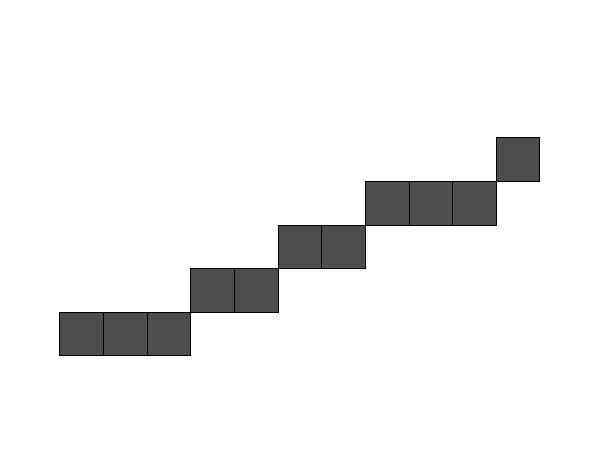
\includegraphics[width=2.5cm]{3_7_0_7}}
    \subfigure[ $\mathcal{D}(3,7,0,8)$]{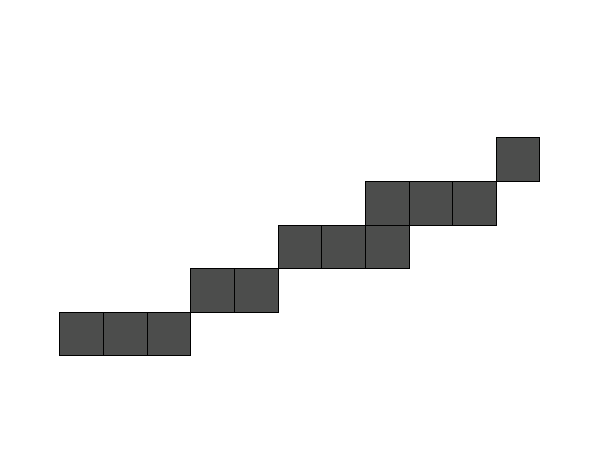
\includegraphics[width=2.5cm]{3_7_0_8}}
    \subfigure[ $\mathcal{D}(3,7,0,10)$]{
\includegraphics[width=2.5cm]{3_7_0_10}}
    \subfigure[ $\mathcal{D}(3,7,0,16)$]{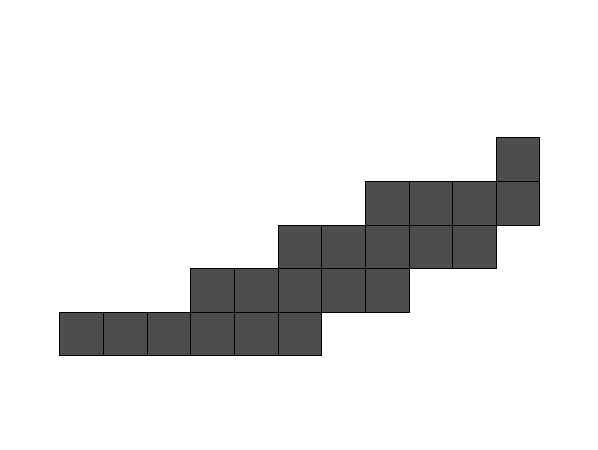
\includegraphics[width=2.5cm]{3_7_0_16}} 
  \end{center}
  \caption[Connexit� des droites discr�tes en fonction de $\omega$]
  {Connexit� des droites discr�tes en fonction de $\omega$~:
    $(a)$ segment d�connect�, $(b)$ segment na�f, $(c)$ segment
    *-connexe, $(d)$ segment standard et $(e)$ segment �pais.}
  \label{fig:epaisseur}
\end{figure}

Nous pouvons faire le lien entre ces droites et les processus de
discr�tisation usuels~:

\begin{prop}[\citealt{reveilles}]
Supposons une droite rationnelle D d'�quation $ax+by+c=0$ avec
$a,b,c$ dans $\Z$, on suppose sans perte de g�n�ralit� que
$b=|b|=max(|a|,|b|)$. Nous avons alors~:
\begin{itemize}
\item la discr�tisation {\it par d�faut} de D, c'est-�-dire l'ensemble
des pixels tel que $ \left \{  (x,y)~|~ y=\left \lfloor \frac{-ax-c}{b}
\right   \rfloor \right    \}$    co�ncide avec  la   droite  discr�te
$\mathcal{D}(a,b,-b-c+1,b)$~;
  
\item \sloppy la discr�tisation {\it par  exc�s} de D, c'est-�-dire l'ensemble
des  pixels tel que $\left  \{ (x,y)~|~  y=\left \lceil \frac{-ax-c}{b}
\right     \rceil   \right  \}$ co�ncide  avec      la droite discr�te
$\mathcal{D}(a,b,-c+1,b)$ ~;

\item la  discr�tisation {\it de  meilleure approximation} (ou GIQ) de
D,   c'est-�-dire l'ensemble des   pixels tel que  $\left \{ (x,y)~|~y=
\left [ \frac{-ax-c}{b}  \right ] \right \}$  co�ncide  avec la droite
discr�te $\mathcal{D}(a,b,-c+1-[\frac{b}{2}],b)$.
\end{itemize}
\end{prop}


Revenons sur la construction des droites arithm�tiques. Avant de
d�tailler les �l�ments qui vont nous servir dans les processus de
reconnaissance, il nous faut d�finir les structures qui nous seront
utiles.

Ainsi, �tant  donn�s $a,~b,~\mu$ et $\omega$ dans $\Z$ avec
$pgcd(a,b)=1$, on appellera {\bf pointill�} de niveau $k$ l'ensemble
des pixels $(x,y)$ v�rifiant
l'�quation diophantienne~:
\begin{displaymath}
  ax-by=k
\end{displaymath}


La structure d'un  pointill� est assez simple, si le point $(x_0,y_0)$
appartient au pointill� de niveau $k$, tous les autres points sont de la forme~:
\begin{displaymath}
  (x,u)=(x_0,y_0) +k'(b,a)
\end{displaymath}
avec $k'$ dans $\mathbb{N}$.
Au niveau des pixels composant ce pointill�, on d�finit le {\bf reste}
$r$ d'un pixel $(x,y)$  selon le couple $(a,b)$ comme �tant un point
du pointill� de niveau $r$. Le terme {\bf reste} vient de la notion
usuelle de reste d'une division enti�re. En effet, nous avons~:
\begin{displaymath}
  r=\left\{ \frac{ax}{b} \right\}
\end{displaymath}

Nous avons maintenant la propri�t� suivante nous permettant de
construire des droites discr�tes � partir de pointill�s. Les deux
items de cette propri�t� sont identiques par d�finition mais ces deux
�critures diff�rentes nous serons utiles par la suite~:

\begin{prop}
  La droite $\mathcal{D}(a,b,\mu,\omega)$ est~:
  \begin{itemize}
    \item la r�union des   pointill�s de niveau $k$ pour $k$ dans
      $[\mu,\mu+\omega[$
    \item l'ensemble des pixels de reste compris entre
      $[\mu,\mu+\omega[$
    \end{itemize}
\end{prop}

Sur cette droite discr�te, nous pouvons encore remarquer des objets
importants. Ainsi, on appellera {\bf droite d'appui inf�rieure} de
$\mathcal{D}$, la droite d'�quation~:
\begin{displaymath}
  ax-by=\mu+\omega-1
\end{displaymath}
Les pixels de cette droite ({\it i.e} les pixels de reste
$\mu+\omega-1$) sont appel�s {\bf points d'appui inf�rieurs}.


De mani�re identique, on appellera {\bf droite d'appui sup�rieure} de
$\mathcal{D}$, la droite d'�quation~:
\begin{displaymath}
  ax-by=\mu
\end{displaymath}
Les pixels de cette droite ({\it i.e} les pixels de reste
$\mu$) sont appel�s {\bf points d'appui sup�rieurs} (voir figure
\ref{fig:reveilles_appui}).

\begin{figure}
  \begin{center}
    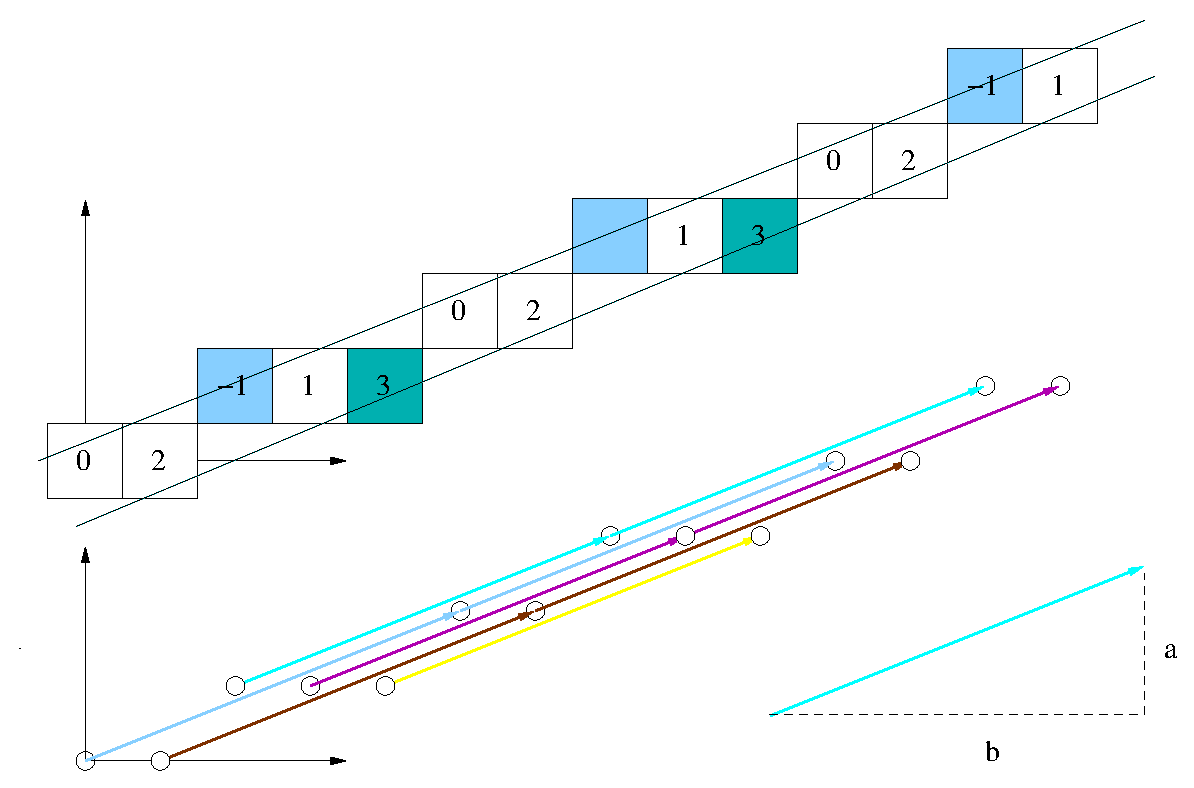
\includegraphics[width=10cm]{Fig/reveilles_appui}
    \caption{Droite discr�te arithm�tique na�ve de param�tres $\mathcal{D}(2,5,-1,5)$~: {\it (haut)}
      repr�sentation  par  restes avec les  points  et droites d'appui
      {\it (bas)} construction par union de pointill�s.}
    \label{fig:reveilles_appui}
  \end{center}
\end{figure}


Certaines notions d'arithm�tique li�es � ces droites apparaissent tr�s
nettement dans la d�finition des restes associ�s � une droite
discr�te. On se place en effet dans un espace modulaire
$modulo~b$, ce qui illustre la notion de  {\it p�riode} $b$ associ�e �
une droite discr�te (qui correspond exactement au param�tre $q$ de
\citealt{Smeulders84}).  


Ces notions  de modularit�  dans    les droites discr�tes  sont   tr�s
anciennes~; en effet \cite{bernoulli},  qui �tait {\it astronome royal},
pr�sente un chapitre dont le titre est {\it  ``Sur une nouvelle esp�ce
de  Calcul''}.    Le  probl�me de    l'�poque   �tait la  construction
d'�ph�m�rides  pour l'astronomie. \aut{Bernoulli} pr�sente une m�thode
tr�s  efficace pour    l'interpolation  lin�aire de   la  position  de
plan�tes. En se ramenant �  des positions enti�res, l'objectif est  de
calculer les valeurs  de  $P$  en  fonction de  $n$ dans  l'expression
$P=\frac{mn}{c}$.

\begin{quote}
  [� propos du calcul d'interpolation classique \citep{bernoulli}] {\it or la M�thode que je
  me propose de rendre compte, satisfait exactement cette condition, \&
  quel que soit le nombre de $n$, on n'a besoin de faire, pour une
  valeur donn�e de $m$, qu'une seule r�gle de trois, tous les autres
  termes se d�terminant par de simples additions, au moyen de certaines
  formules g�n�rales que j'ai trouv�es ; \& cette m�thode est d'une telle
  facilit� dans l'application, qu'on est souvent en �tat d'�crire,
  sans autre calcul, les produits de plus de 1000 r�gles de trois, en
  deux heures de temps.}
\end{quote}

Il �met ensuite l'observation suivante~:

\begin{quote}
  {\it On peut remarquer que la diff�rence pour ces augmentations des
    $P$ ne roulera jamais que sur une unit� de plus ou de moins ;
    c'est � dire que si $m=x+\frac{a}{c}$, ce sera toujours ou $x$ ou
    $x+I$ unit�s qu'il faudra ajouter au dernier chiffre � mesure que
    $n$ cro�t de I.}

  \end{quote}
  
En d'autres termes, si $n$ et $P$ sont respectivement des abscisses et
des ordonn�es, les pixels successifs pour $x$ croissant, appartenant �
 la droite d�crite par la pente $\frac{m}{c}$, sont constitu�s en {\it
   palier} avec des d�crochements diagonaux entre ceux-ci. 

Il montre ensuite l'aspect p�riodique de ces d�crochements~:



\begin{quote}
  {\it De plus, si on entend par $\frac{h}{k}$ la fraction
    $\frac{a}{c}$ r�duite � ses moindres termes, ou que $\frac{m}{c}=
    x+\frac{a}{c}=x=\frac{h}{k}$ ; il ne m'a pas �t� difficil 
    de prouver, qu'au bout d'une p�riode de $k$ termes les
    augmentations de $P$ doivent revenir dans le m�me ordre ; c'est �
    dire que si on nomme $\Pi$ le terme correspondant � $n+k$, il faudra
    ajouter � $\Pi$, pour $n+k+I$, le m�me nombre d'unit�s qu'on avait
    ajout� � $P$ pour $n+I$}[...].
\end{quote}

Il    propose   ensuite un  calcul   bas� sur   la fraction  continue  de
$\frac{h}{k}$ pour construire   explicitement  tous les  pixels de  la
droite discr�te (voir \citealt{hardy} pour un  compl�ment sur ces notions
d'arithm�tique    et de th�orie  des   nombres).  Ce premier travail a
ensuite �tait repris par  \citet{christoffel} qui construit un mot qui,
par  une  transformation  simple,  se  ram�ne   � une  droite  discr�te
arithm�tique \citep{reveilles}.

\label{sec:bezout}
 
Apr�s cette parenth�se historique, revenons sur la construction de ces
objets. Nous illustrons la puissance de ce formalisme  en donnant une
interpr�tation graphique du th�or�me de \aut{Bezout}, tr�s classique
en arithm�tique~:
\begin{displaymath}
  \forall a,b\in\mathbb{N},\quad \exists u,v\in\mathbb{N}~:~au+bv=pgcd(a,b) 
\end{displaymath}
Dans notre analyse, $a$ et $b$ sont des premiers entre eux, on consid�re
$u$ et $v$ les coefficients de \aut{Bezout} donn�s par:
\begin{displaymath}
  au-bv=1
\end{displaymath}

Ainsi, si $(x_0,y_0)$ appartient au pointill� de niveau $k$, les
autres points de m�me reste sont g�n�r�s par application du vecteur
$(b,a)^T$. Un {\it vecteur de Bezout} $(u,v)^T$ nous permet de passer
d'un pointill� � un autre. En effet, tous les vecteurs de la forme
$(u,v)^T+k'(b,a)^T$ avec $k'$ dans $\Z$  nous permettent de
passer d'un point du pointill� $k$ � un point du pointill� $k+1$. Pour
cela, supposons $ax_0-by_0=k$ puis~:

\begin{align*}
  a(x_0+u+k'b) - b(y_0+v+k'a) &= ax_0-by_0 +au-bv + abk'-abk'\\
  &= ax_0-by_0 +1\\
  &= k+1
\end{align*}

\begin{figure}
  \begin{center}
    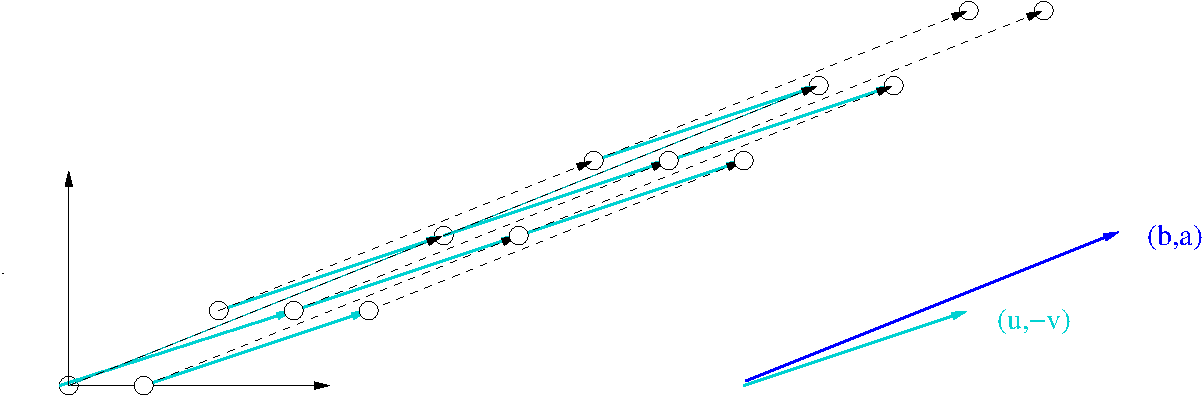
\includegraphics[width=10cm]{Fig/droites_bezout}
    \caption{Pointill�s et vecteur de Bezout pour la droite  $\mathcal{D}(2,5,-1,5)$.}
    \label{fig:droites_bezout}
  \end{center}
\end{figure}

Par exemple, la figure \ref{fig:droites_bezout} illustre les vecteurs
g�n�rant la droite $\mathcal{D}(2,5,-1,5)$ tels que $(b,a)^T=(5,2)^T$
et $(u,v)^T=(3,1)^T$. Ainsi, la construction d'une droite discr�te se
fait, en partant d'un point de reste $\mu$, par application de
$\omega-1$ fois le vecteur de Bezout pour passer  d'un pointill� �
l'autre et autant de fois le vecteur $(b,a)$ qu'il faut dans chaque
pointill�. Nous  utiliserons  cette notion de vecteur de Bezout dans
la partie reconnaissance de cercles (chapitre \ref{chap-cercles}).


\subsubsection{Quelles {\it droites} choisir ?}

De  nombreuses autres d�finitions   de droites discr�tes existent,  le
lecteur pourra se r�f�rer �  l'article  de \cite{rosen_klette} ou  aux
th�ses soutenues sur ce sujet comme celles de \cite{debledthese} ou de
\cite{vialardthese}. Cependant,   la    majorit� de  ces   d�finitions
d�signe le m�me objet g�om�trique.  Dans ce que nous avons pr�sent�,
nous avons l'�quivalence entre les d�finitions suivantes~:
\begin{itemize}
\item les propri�t�s de \aut{Freeman} formalis�es par \citeauthor{wu}
  et \citeauthor{HUE_1981}~;
\item la propri�t� de corde de \aut{Rosenfeld}~:
\item la propri�t� de r�gularit� de \citeauthor{Hung85}~;
\item le quadruplet $(n,q,p,s)$ de  \citeauthor{Smeulders84}~;
\item la notion de droite arithm�tique avec comme �paisseur $\omega=max(|a|,|b|)$.
\end{itemize}
 

Le choix de telle ou telle approche est dirig� par l'algorithmique que
l'on applique � ces d�finitions. Par exemple, si notre objectif est le
trac� de droite, la propri�t� de corde ne nous permet pas d'�crire des
algorithmes efficaces alors que les droites arithm�tiques le
permettent.  De m�me, dans un objectif de reconnaissance de droite, on
adoptera la m�thode la plus simple � impl�menter. 

\subsubsection{Trac� de droites discr�tes}

Nous pr�sentons les algorithmes classiques de trac� de droites
discr�tes que nous utiliserons par la suite.  

Nous  commen�ons par    un     algorithme tr�s  connu     propos�  par
\cite{bres65}.   Le  cadre de    ce  travail  est le   suivant~:  nous
consid�rons deux points de la grille  not�s $(x_0,y_0)$ et $(x_1,y_1)$
et l'on souhaite tracer le segment de droite joignant ces deux pixels.
Nous   pouvons, sans perte de  g�n�ralit�,  nous placer  dans le premier
octant, c'est-�-dire   $x_1-x_0>y_1-y_0>0$. Nous illustrerons   par la
suite les transformations permettant de g�n�raliser  le trac� dans les
autres octants.

L'id�e  de   cet algorithme est le   suivant~:  nous allons tracer les
pixels de $x_i$ vers $x_f$ dans cet ordre. A chaque �tape, nous devons
choisir entre rester sur le m�me {\it palier}  ({\it i.e.} rester � la
m�me ordonn�e)  ou aller en diagonale.  Pour  cela, nous propageons une
mesure d'erreur  nous permettant de  toujours choisir le pixel le plus
proche. Nous obtenons donc l'algorithme \ref{alg:bresenham}.



\begin{algorithm}
\caption{Trac� de droite de \cite{bres65}}
\label{alg:bresenham}
\begin{algorithmic}[1]
\EXTERNNAME \INTERNNAME{trac�\_Bresenham($x_0,y_0,x_1,y_1$)}

\STATE $dx=x_1-x_0$, $dy=y_1-y_0$
\STATE $x=x_0$, $y=y_0$
\STATE $incrHor=2dy$, $incrDiag=2(dx-dy)$
\STATE $e=2dy-dx$

\FOR{$x$ allant de $x_0$ � $x_1$}
\STATE \INTERNNAME{Afficher\_pixel}(x,y)
\IF{$e\geq 0$}
\STATE $y\texttt{+=}1$
\STATE $e\texttt{+=}incrDiag$
\ELSE
\STATE $e\texttt{+=}incrHor$
\ENDIF
\ENDFOR
\end{algorithmic}
\end{algorithm}


Nous d�taillons aussi l'algorithme de trac� des droites discr�tes
arithm�tiques. Nous nous int�ressons plus particuli�rement aux droites
arithm�tiques na�ves. Comme nous l'avons remarqu� pr�c�demment, la
structure modulaire du reste dans la droite discr�te permet de
comprendre enti�rement la structure g�om�trique de la droite. Il est
donc naturel de baser l'algorithme de trac� sur cette
information. Nous obtenons donc l'algorithme
\ref{alg:trace_reveilles}. Cet algorithme est tr�s similaire � celui
de \citeauthor{bres65}, en fait,  l'algorithme \ref{alg:bresenham} est
une instance de cet algorithme pour $\mu=\left [ \frac{x_f-x_i}{2}
\right ]+1$ (voir \citealt{debledthese}).

\begin{algorithm}
\caption{Trac� de droites arithm�tiques na�ves de \cite{reveilles} et \cite{debledthese}}
\label{alg:trace_reveilles}
\begin{algorithmic}[1]
\EXTERNNAME \INTERNNAME{trac�\_arithm�tique($x_0,y_0,x_1,y_1,\mu$)}
\STATE $v_x=x_1-x_0$, $v_y=y_1-y_0$
\STATE $r=v_yx_0-v_xy_0-\mu$
\STATE $x=x_0$, $y=y_0$
\WHILE{$x<x_b$}
\STATE $x\texttt{+=}1$
\STATE $r\texttt{+=}v_y$
\IF{$r<0$ ou $r\geq v_x$}
\STATE $y\texttt{+=}1$
\STATE $r\texttt{-=}v_x$
\ENDIF
\STATE \INTERNNAME{Afficher\_pixel}(x,y)
\ENDWHILE
\end{algorithmic}
\end{algorithm}

D'autres  algorithmes de trac�  pour   les droites arithm�tiques  {\it
�paisses}  ont  �t� propos�s par \cite{reveilles}      mais nous ne  les
utiliserons pas par la suite.


Pour g�n�raliser ce trac� dans tous les octants, nous utilisons, au
niveau de la fonction  \INTERNNAME{Affiche\_pixel}, les
transformations du tableau \ref{tab:oct}. Le nombre de tests �
effectuer dans l'impl�mentation est encore suffisamment raisonnable
pour envisager une impl�mentation directe du tableau
\ref{tab:oct}. Nous verrons par la suite comment nous r�solvons le probl�me
en 3D o� 48 cas sont � g�rer.

\begin{table}[htbp]
  \centering
  \begin{tabular}{|c|c|}
    \hline
    Octants & Transformations de $(x,y)$\\
    \hline
    1 & $(x,y)$\\
    2 & $(y,x)$\\
    3 & $(y,-x)$\\
    4 & $(x,-y)$\\
    5 & $(-x,-y)$\\
    6 & $(-y,-x)$\\
    7& $(-y,x)$\\
    8 & $(-x,y)$\\
    \hline
  \end{tabular}
  \caption{Transformations pour la g�n�ralisation du trac� de droite dans tous les octants.}
  \label{tab:oct}
\end{table}



\subsection{Reconnaissance et segmentation}

Dans cette partie, nous nous int�ressons aux algorithmes permettant de
d�cider  si un  ensemble de points  discrets  appartient ou non �  une
droite discr�te. De mani�re plus  pr�cise, nous pouvons d�composer  le
probl�me en deux grands axes~:
\begin{description}
\item[Test de lin�arit�] : pr�dicat permettant de d�cider si un
  ensemble de pixels forme un segment discret.

\item[Reconnaissance de la droite] : cette fois, non seulement nous
  d�cidons si un ensemble de pixels appartient � une droite
  discr�te, mais nous obtenons les param�tres de cette droite discr�te.
\end{description}

Quel que soit le probl�me choisi, nous �valuons les diff�rents
algorithmes selon les crit�res suivants~:
\begin{description}
\item[Conditions sur l'ensemble  de pixels] : est-ce que  l'algorithme
�met    des hypoth�ses sur    la structure   de l'ensemble  de  pixels
(connexit�, tri sur un axe de coordonn�es\ldots) ?
\item[Complexit�]   : mesur�e en   fonction du   nombre  de pixels  de
l'ensemble   � reconna�tre.   Nous  nous  int�ressons   aussi �   la
complexit� en m�moire de chaque algorithme.
\item[Difficult� d'impl�mentation] : d'un point de vue pratique,
  est-ce que la m�thode se programme facilement ?
\end{description}


Dans   la   litt�rature,   \cite{rosen_klette}  attribuent   le  premier
algorithme de reconnaissance de droite   discr�te en temps lin�aire  �
\cite{HUE_1981}. Cependant, le probl�me peut �tre abord� par tellement
d'approches diff�rentes que  cela rend toute classification historique
difficile.

Dans ce  qui suit, nous d�taillerons deux  grandes  approches pour la
reconnaissance qui seront utilis�es par la suite. Le lecteur pourra se
r�f�rer � \cite{rosen_klette} pour une bibliographie plus large sur le
sujet.



\subsubsection{Approche bas�e sur la structure du dual}
\label{sec:approche-dual}


A partir du codage $(n,q,p,s)$  des droites discr�tes,
\cite{Smeulders84} construisent la {\it pr�-image} associ�e � une droite
discr�te. Cette pr�-image est un domaine, dans l'espace des
param�tres, qui repr�sente l'ensemble des droites r�elles dont la
discr�tisation contient l'ensemble des pixels du segment discret
consid�r�.

De mani�re plus formelle, nous consid�rons tout d'abord un segment de
droite discr�te na�ve dans le premier octant, not�
$\mathcal{S}$. D'apr�s les d�finitions vues au paragraphe
\ref{sec:defin-et-propr}, il existe alors un couple
$(\alpha,\beta)\in[0,1]\times[0,1[$ tel que $\mathcal{S}$ est contenu
dans la discr�tisation de  la droite $y=\alpha x+\beta$.

Nous notons $\bar{\mathcal{S}}$ l'ensemble de ces droites donn� par~:
\begin{equation}
\label{eq:dual}
  \bar{\mathcal{S}}=\{(\alpha,\beta\})\in[0,1]\times[0,1[~|~
  \forall (x,y)\in\mathcal{S},~0\leq \alpha x+\beta -y <1 \}
\end{equation}


Si nous d�composons la construction de $\bar{\mathcal{S}}$, chaque
pixel de $\mathcal{S}$ engendre, dans l'espace dual $(\alpha,\beta)$
un bande semi-ouverte d�finie par~:

\begin{displaymath}
  \mathcal{B}(x,y)=\left \{ \begin{array}{l}
\alpha x + \beta -y \geq 0\\
\alpha x + \beta -y < 1
\end{array}
\right .
\end{displaymath}


�tant donn� que  $\bar{\mathcal{S}}$ est une intersection de
contraintes lin�aires, ce domaine est convexe dans l'espace des
param�tres (voir figure \ref{fig:dual_exemple}).

\begin{figure}
  \begin{center}
    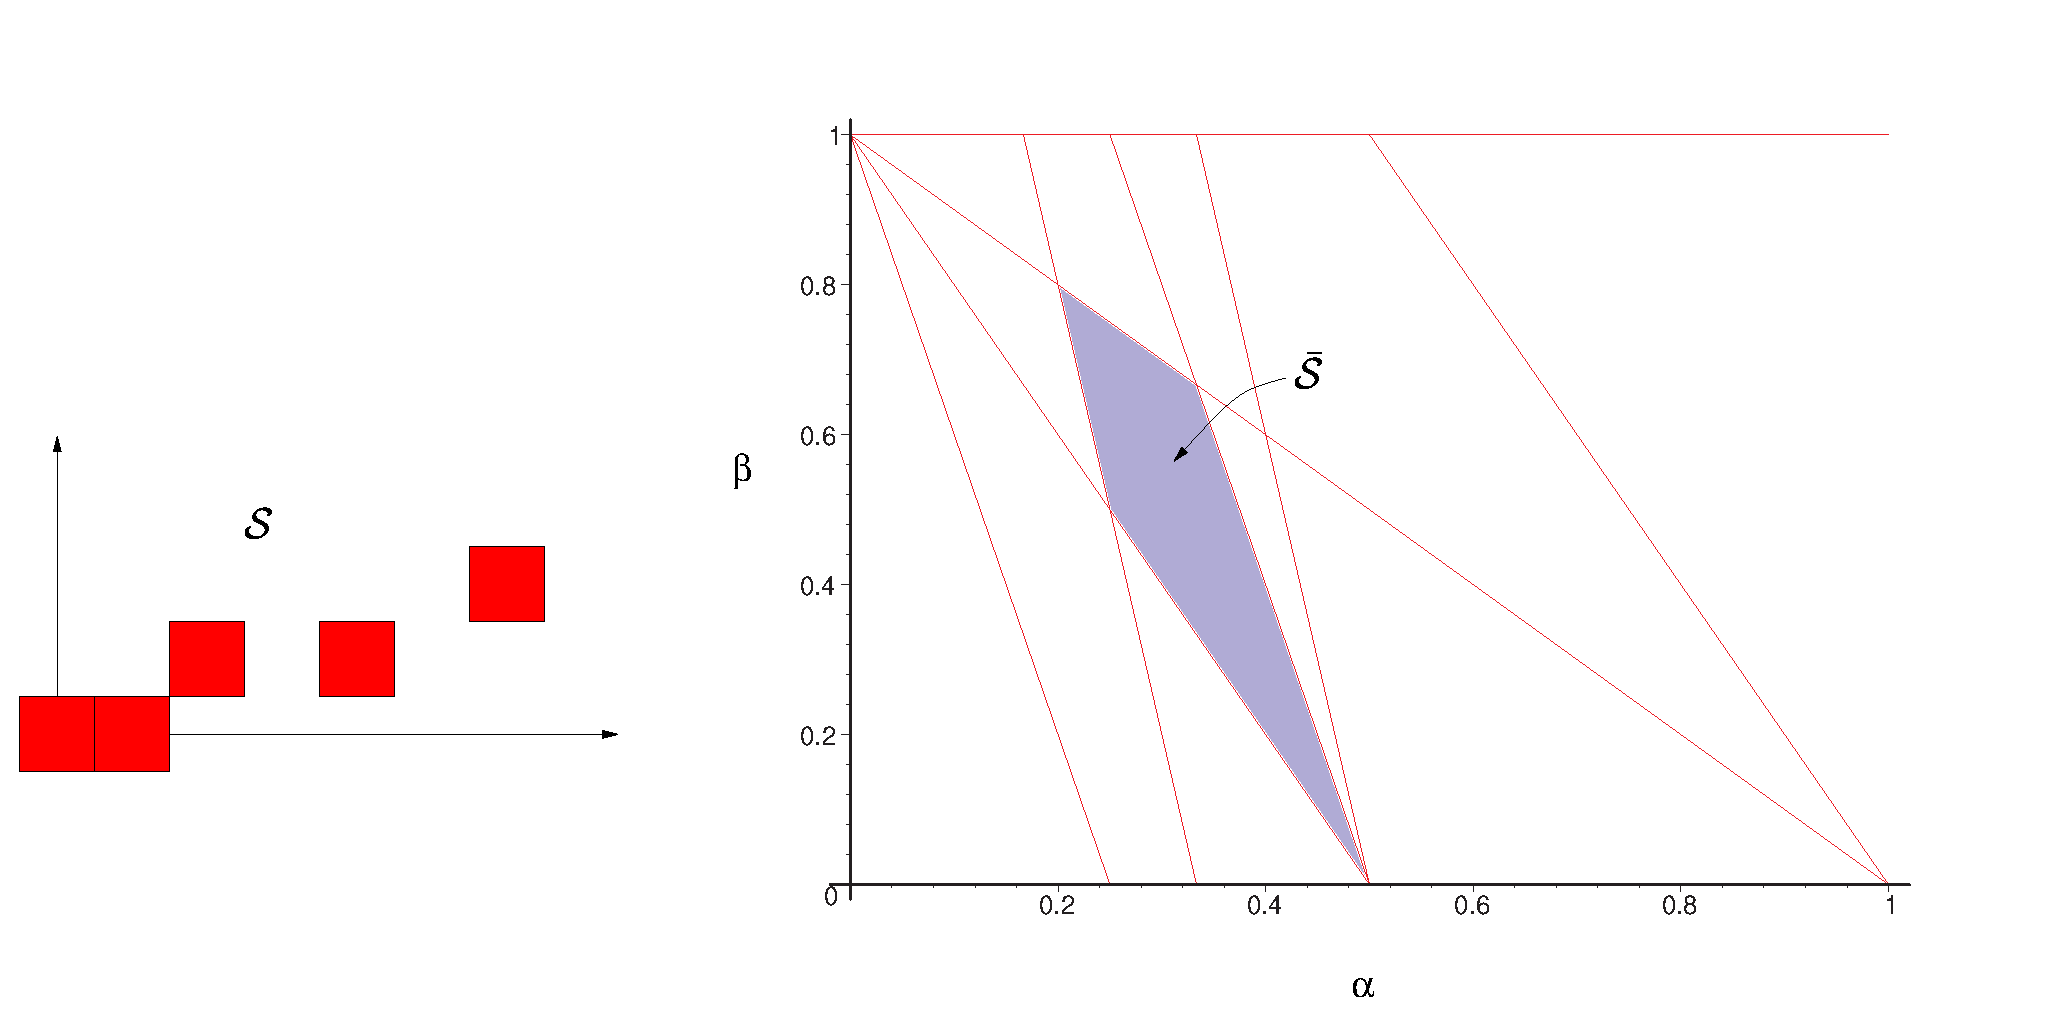
\includegraphics[width=12cm]{Fig/dual_exemplebis.ps}
    \caption{Ensemble de pixels $\mathcal{S}$ et domaine des droites
      euclidiennes      $y=\alpha      x  +\beta$     associ�es, not�
      $\bar{\mathcal{S}}$.}
    \label{fig:dual_exemple}
  \end{center}
\end{figure}


Pr�sent� en ces termes, le probl�me se ram�ne donc � un probl�me
classique de programmation lin�aire~: �tant donn� un syst�me de
contraintes lin�aires, nous voulons  soit d�cider si le syst�me est
valide (c'est-�-dire s'il existe au moins une solution), soit calculer
le polytope solution dans l'espace des param�tres.

De nombreux algorithmes existent pour r�soudre ce probl�me quelque
soit la dimension des contraintes (c'est-�-dire la dimension de l'espace
des param�tres). De mani�re g�n�rale, nous avons le th�or�me suivant
nous permettant d'avoir une borne sur la complexit� asymptotique du
test de lin�arit�~:

\begin{theo}[\cite{megiddo}]
\label{theo:megiddo}
  �tant  donn� un syst�me de  $n$  in�quations  lin�aires de dimension  $d$,
  tester si un syst�me admet une solution  se calcule en temps optimal
  pour une dimension fixe, c'est-�-dire en $O(n)$.
\end{theo}
 
Le probl�me majeur de cette approche est la  constante importante
devant cette complexit� asymptotique. En effet, celle-ci est
exponentielle en la dimension. Cependant, dans le cas de faible
dimension, l'algorithme de \cite{megiddo} offre une solution tr�s
efficace. 
Dans notre cas, le test de lin�arit� d'un ensemble de pixels engendre
un syst�me de $2n$ in�quations de dimension 2 (o� $n$ est le nombre de
pixels). Nous obtenons donc une solution optimale en temps,
c'est-�-dire $O(n)$, � notre premier probl�me. R�cemment, \cite{buzer}
a pr�sent� une version incr�mentale de cet algorithme toujours en
temps optimal quelle que soit la dimension. 

Si nous souhaitons d�crire tous  les sommets du domaine solution,  des
algorithmes tr�s efficaces existent pour  les  dimensions 2 et 3.  Ces
algorithmes viennent  g�n�ralement d'une r�solution du probl�me dual~:
en dimension 2, la  transform�e   dans l'espace des  param�tres  d'une
droite est un  point, la transform�e d'un  point est une droite et une
in�quation lin�aire  se  transforme aussi en  une  contrainte lin�aire
dans  le dual mais   calculer le polytope  des  solutions d'un syst�me
d'in�quation se  ram�ne � un  calcul d'enveloppe convexe  dans le dual
(voir \citealt{boissonnat,deberg} et figure \ref{fig:passage_dual}).

\begin{figure}
  \begin{center}
    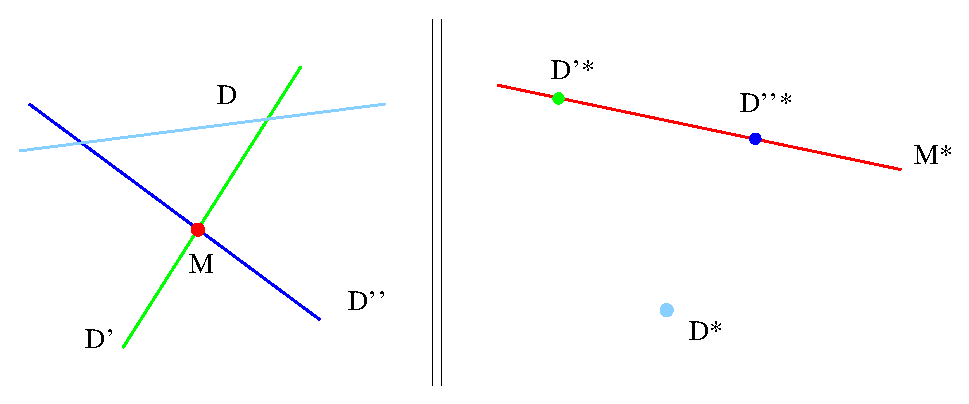
\includegraphics[width=10cm]{Fig/fig1rbis}
    \caption[Passage dans l'espace des param�tres associ�s aux
    droites]{Passage  dans  l'espace   des  param�tres   associ�s  aux
    droites~:  les  droites  $D$,    $D'$ et   $D''$  {\it(�  gauche)}
    deviennent respectivement les points $D^*$, $D'^*$ et $D''^*$ {\it
    (� droite)}, le point $M$ devient la droite $M^*$. $M$ satisfait
    la contrainte lin�aire $D$ implique que $D^*$  est en  dessous de
    $M^*$ dans l'espace dual.}
    \label{fig:passage_dual}
  \end{center}
\end{figure}

Ainsi, les   bornes  des algorithmes  de  calcul d'enveloppes convexes
impliquent des   bornes sur le calcul du    domaine des solutions d'un
syst�me.   Pour la dimension  2, \cite{P16} ont pr�sent� un algorithme
optimal dont la  borne est en $O(nlog(n))$. Pour  ne pas surcharger ce
chapitre, l'algorithme optimal  de  \cite{P16} est pr�sent� en  annexe
(voir annexe \ref{chap:annexe_prog}).

Finalement, sans aucune prise en compte de l'aspect g�om�trique ou des
propri�t�s  des  droites discr�tes,  nous  avons  des algorithmes tr�s
efficaces pour le  test de lin�arit� ou  la reconnaissance  de droites
discr�tes.  Ces bornes  sont certes  int�ressantes mais l'introduction
de la particularit�  des    droites discr�tes permet    de  simplifier
consid�rablement les bornes et les algorithmes.

Avant de pr�senter un premier algorithme de reconnaissance optimal, il
nous  faut   revenir sur une   illustration g�om�trique  de l'�quation
\ref{eq:dual}.  Ainsi,   l'ensemble  des solutions $\bar{\mathcal{S}}$
correspond �  l'ensemble des  droites passant  par tous  les  segments
semi-ouverts $[MM'[$ o�   $M=(x,y)$ et  $M'=(x,y+1)$ pour tous    les
points  $(x,y)$  de  $\mathcal{S}$ (voir figure  \ref{fig:intervals}).
Cette r��criture   du probl�me  est   �vidente mais elle  nous  permet
d'appliquer un  algorithme  tr�s  efficace  propos�  par \cite{rourke}
permettant de d�crire l'ensemble  des droites  r�elles passant par  un
ensemble d'intervalles d�finis sous la forme $[(x,\alpha),(x,\omega)]$
(voir figure \ref{fig:algo_rourke})

\begin{figure}
  \begin{center}
    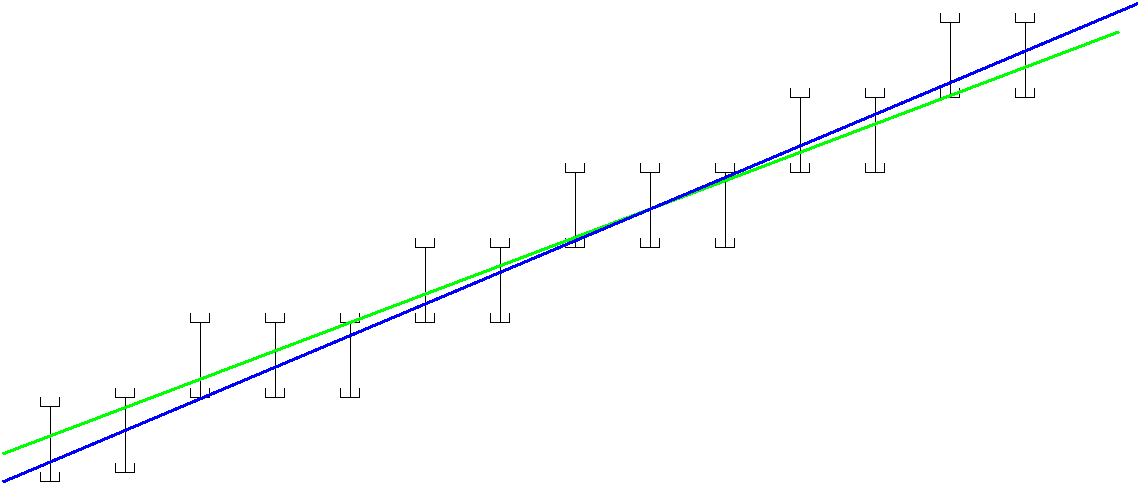
\includegraphics[width=10cm]{Fig/intervalle_OBQ}
    \caption{Repr�sentation de la droite discr�te
      $\mathcal{D}(2,5,-1,5)$ sous forme d'intervalles et droites
      euclidiennes solutions.}
    \label{fig:intervals}
  \end{center}
\end{figure}

Ainsi,  \citeauthor{rourke}   pr�sente   un  algorithme incr�mental et
optimal en temps pour  d�crire  le domaine  de l'ensemble des  droites
passant par   ces intervalles  (voir  figure \ref{fig:algo_rourke})  :
�tant donn� un ensemble   de $n$  intervalles  tri�s selon  l'axe  des
abscisses,    le  calcul du domaine    des  droites  dans l'espace des
param�tres  se   calcule  en   $O(n)$.    De plus, pour     tout ajout
d'intervalle croissant en $x$,  la mise � jour  du domaine se  fait au
pire cas  en $O(n)$ mais   l'analyse amortie de  ce  calcul montre une
complexit� optimale pour le probl�me.

\begin{figure}
  \begin{center}
    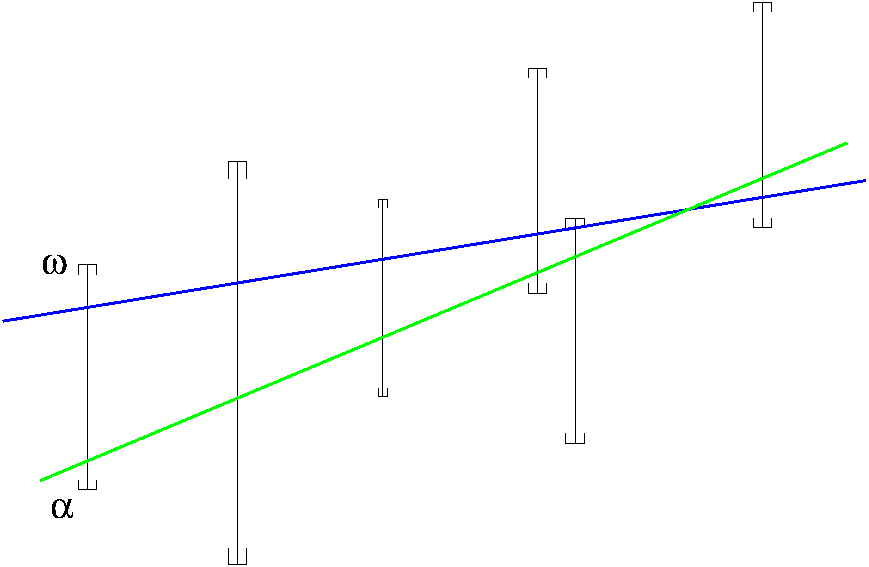
\includegraphics[width=6cm]{Fig/orourke}
    \caption{Algorithme de \citeauthor{rourke} pour construire
      l'ensemble des droites r�elles passant par une s�rie d'intervalles.}
    \label{fig:algo_rourke}
  \end{center}
\end{figure}


En consid�rant donc une description de $\mathcal{S}$ sous forme d'une
liste cha�n�e de pixels (description en $k-$arcs), nous avons ramen�
la complexit� de $O(nlog(n))$ � $O(n)$. 

%Nous reviendrons sur cet algorithme plus tard.


En ajoutant la contrainte de connexit�, nous obtenons une borne
optimale en temps et en m�moire � nos deux probl�mes. Ainsi, lors de
la caract�risation en $(n,q,p,s)$, \cite{Smeulders84} ont montr� le
th�or�me suivant~:

\begin{theo}[Structure du domaine des droites discr�tes]
\label{theo:structure1}
 �tant donn� un ensemble de pixels $\mathcal{S}$ connexes, le domaine
$\bar{\mathcal{S}}$ dans l'espace des param�tres a, au plus, 4 sommets.
\end{theo}

La preuve de ce th�or�me a �t� pr�sent�e par \citeauthor{Smeulders84}, 
et ind�pendamment, \cite{ilroy} a propos�, la m�me ann�e, une preuve
tr�s simple concernant la propri�t� de structure du dual.

En plus de  ce r�sultat sur le nombre   de sommets dans le  dual, ces
sommets ont  une structure arithm�tique  tr�s int�ressante. Tout
d'abord, rappelons  les  notions de  s�ries de  Farey  en th�orie  des
nombres (voir par exemple \citealt{hardy})~:

\begin{defi}[Serie de Farey]
  Une s�rie de Farey d'ordre $n\in\mathbb{N^*}$ est l'ensemble des fractions
irr�ductibles ordonn�es de l'intervalle [0,1] dont les d�nominateurs sont
inf�rieurs � $n$.
\end{defi}

Par exemple, la s�rie de Farey d'ordre 5 est l'ensemble~:
\begin{displaymath}
\mathcal{F}_5=\left
  \{\frac{0}{1},\frac{1}{5},\frac{1}{4},\frac{1}{3},\frac{2}{5},\frac{1}{2},\frac{3}{5},\frac{2}{3},\frac{3}{4},\frac{4}{5},\frac{1}{1}\right \}
\end{displaymath}

Sur ces s�ries, nous avons les propri�t�s suivantes~:
\begin{prop}
  �tant donn�e $\mathcal{F}_n$ la s�rie de Farey d'ordre $n$, nous
  avons~:
  \begin{itemize}
  \item si $\frac{h}{k}$ et $\frac{h'}{k'}$  sont deux membres
    cons�cutifs de $\mathcal{F}_n$, alors $kh'-hk'=1$
\item si $\frac{h}{k}$, $\frac{h''}{k''}$ et  $\frac{h'}{k'}$  sont
  trois termes cons�cutifs de  $\mathcal{F}_n$, alors
  $\frac{h''}{k''}=\frac{h+h'}{k+k'}$. Ce point est appel� le {\bf
    m�dian} de  $\frac{h}{k}$ et $\frac{h'}{k'}$.
  \end{itemize}
\end{prop}

Les  s�ries de Farey peuvent se  calculer de mani�re r�cursive.  La
s�rie  $\mathcal{F}_{n+1}$   se construit,  �    partir de   la  s�rie
$\mathcal{F}_{n}$, en  ajoutant tous les  points m�dians des fractions
cons�cutives de $\mathcal{F}_n$ dont les d�nominateurs sont inf�rieurs
� $n+1$.

Ainsi, pour construire la s�rie d'ordre 6, nous ajoutons
� $~\mathcal{F}_5$ les fractions $\frac{1}{6}$ et   $\frac{5}{6}$ (tous
les autres m�dians sont d�j� dans la liste). Nous obtenons donc~:

\begin{displaymath}
\mathcal{F}_6=\left
  \{\frac{0}{1},\frac{1}{6},\frac{1}{5},\frac{1}{4},\frac{1}{3},\frac{2}{5},\frac{1}{2},\frac{3}{5},\frac{2}{3},\frac{3}{4},\frac{4}{5},\frac{5}{6},\frac{1}{1}\right \}
\end{displaymath}

En se  basant sur ces d�finitions et  propri�t�s  des s�ries de Farey,
nous pouvons compl�ter le th�or�me \ref{theo:structure1} en sp�cifiant
encore la structure de l'espace dual associ� aux droites discr�tes~:

\begin{theo}[\cite{ilroy,Smeulders84}]
 \label{theo:structure2}
 �tant  donn� un ensemble $\mathcal{S}$  de $N+1$ pixels connexes dont
 l'abscisse     minimale   des   points   est      $x_0$, le   domaine
 $\bar{\mathcal{S}}$ dans l'espace des param�tres est tel que~:
\begin{itemize}
\item il a au plus 4 sommets~;
\item les abscisses de ces sommets appartiennent � la Farey d'ordre $\max(x_0,N-x_0)$~;
\item si le domaine a 4 sommets, deux d'entre eux ont la m�me abscisse~;
\item les abscisses  de deux sommets adjacents sont des fractions
  cons�cutives dans une s�rie de Farey~;
\item si l'abscisse d'un sommet est $\frac{p}{q}$, l'ordonn�e de
  celui-ci est un multiple de $\frac{1}{q}$.
\end{itemize}
\end{theo}

\begin{figure}[htbp]
  \begin{center}
    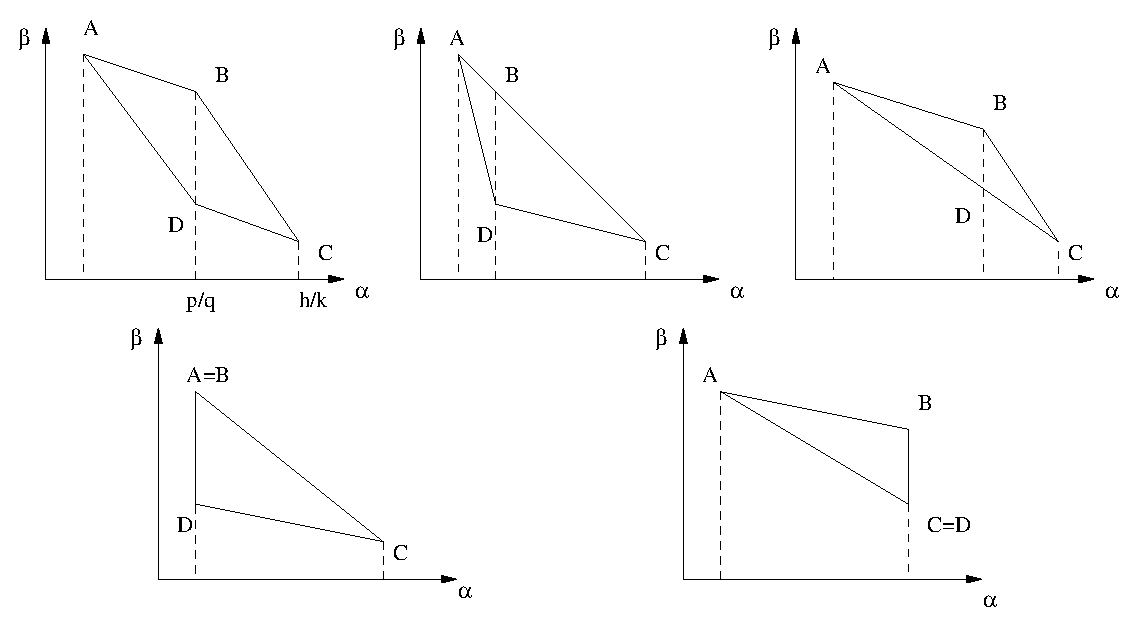
\includegraphics[width=10cm]{Fig/structure_ilroy}
   \caption{Diff�rentes formes du domaine des droites dans le dual.}
    \label{fig:structure}
  \end{center}
\end{figure}


En consid�rant toutes  ces propri�t�s, le  domaine des solutions  dans
l'espace   dual  ne   peut   prendre  que    cinq formes  diff�rentes,
repr�sent�es  figure \ref{fig:structure}. Pour  illustrer la quatri�me
propri�t� de  ce domaine,  dans le cas  du quadrilat�re  de  la figure
\ref{fig:structure}, les fractions $\frac{p}{q}$ et $\frac{h}{k}$ sont
adjacentes dans la s�rie de Farey associ�e au domaine.

D'une mani�re encore  plus  pr�cise, \cite{ilroy} introduit  la notion
{\it d'�ventail de Farey} (de l'anglais {\it Farey fan}) permettant de
d�crire toutes les formes possibles de $\bar{\mathcal{S}}$ en fonction
de  l'ordre de Farey  associ� �  la  droite.  En d'autres termes,  un
polygone de  ce  diagramme  d'ordre $q$   contenu dans   le  rectangle
$[0,1]\times[0,1]$, appel� {\it  cellule  de Farey},  correspond  � la
pr�-image    d'un    segment     discret      de    longueur     $q+1$
\citep{ilroy,vittonethese}.   La figure \ref{fig:farey_fans}  illustre
ce calcul pour l'ordre 2, 3 et 6~: toutes les  {\it cellules de Farey}
contenues dans le   rectangle $[0,1]\times[0,1]$  sont l'ensemble  des
domaines possibles  pour tout ensemble  de pixels g�n�rant un ordre de
Farey de 2, 3 ou 6.  Ainsi, dans la figure \ref{fig:farey_fans}$-(c)$,
on remarque  que tous ces  polygones sont de la   forme d�crite dans le
th�or�me \ref{theo:structure2}.

\begin{figure}[htbp]
  \begin{center}
    \subfigure[]{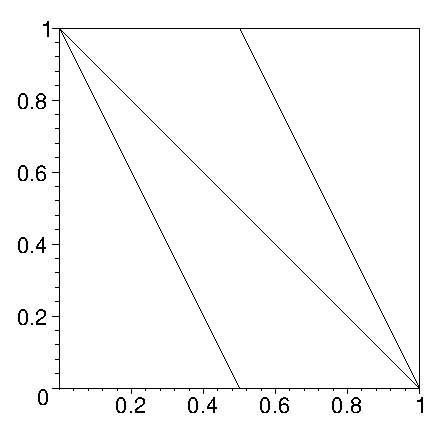
\includegraphics[width=6cm]{Fig/farey_fan_2}}
    \subfigure[]{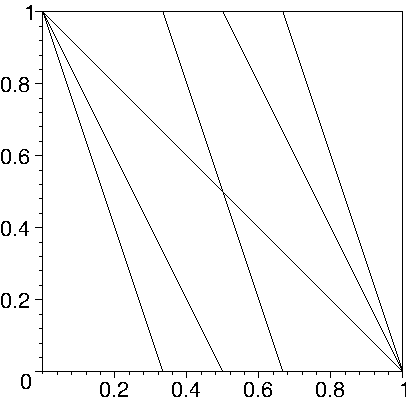
\includegraphics[width=6cm]{Fig/farey_fan_3}}
    \subfigure[]{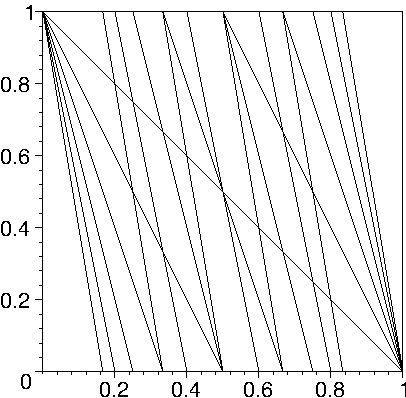
\includegraphics[width=6cm]{Fig/farey_fan_6}}
    \caption[Illustration des �ventails de Farey introduits par
\cite{ilroy}]{Illustration  des  �ventails  de  Farey   introduits par
\cite{ilroy}~:  $(a)$ �ventail d'ordre  2, $(b)$ �ventail d'ordre 3 et
$(c)$  �ventail  d'ordre 6.  Les polygones   d�finis dans le rectangle
$[0,1]\times[0,1]$ correspondent aux  domaines possibles associ�s  aux
segments discrets.}
    \label{fig:farey_fans}
  \end{center}
\end{figure}


Si nous  oublions les propri�t�s  arithm�tiques du  domaine dual, nous
pouvons d�j� proposer des algorithmes  optimaux en temps et en m�moire
pour la reconnaissance de segments discrets.  En  effet, �tant donn� que
ce polygone  des  solutions ne  peut   avoir plus de   4 sommets, nous
pouvons calculer la  nouvelle  forme de  ce domaine, apr�s   insertion
d'une nouvelle contrainte, en temps constant.

Cependant,   la structure arithm�tique   nous  permet de maintenir  ce
polygone sous  forme  irr�ductible, c'est-�-dire   tel  que tous   les
sommets s'�crivent  sous forme de   fractions irr�ductibles.  Pour cela,
\cite{ilroy}   a   d�crit  l'ensemble   des  coupures  possibles apr�s
l'insertion d'un nouveau pixel~:

\begin{theo}
   �tant  donn�  un ensemble de pixels  $\mathcal{S}$   connexes et la
   cellule de Farey qui lui est associ� d'ordre  $q$, si nous ajoutons
   un pixel qui engendre  une contrainte dans l'espace  des param�tres
   intersectant $\bar{\mathcal{S}}$, celle-ci ne  peut pas couper deux
   ar�tes adjacentes ni deux ar�tes oppos�es. De  plus si la contrainte
   coupe une ar�te,  par   exemple $[AB]$, du  domaine,  l'abscisse de
   cette intersection est le  successeur  de l'abscisse de $A$  (resp.
   pr�d�cesseur de  l'abscisse de $B$) dans la  s�rie de Farey d'ordre
   $q+1$.
\end{theo}


\begin{figure}[htbp]
  \begin{center}
    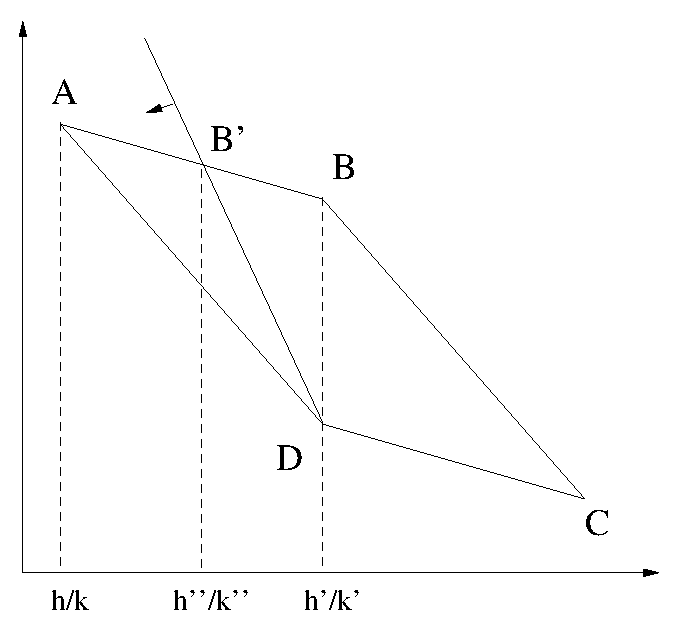
\includegraphics[width=6cm]{Fig/coupure_ilroy}
    \caption{L'ajout d'un nouveau point introduit une contrainte sur
      $\bar{\mathcal{S}}$ d'ordre $q$, le point $B'$ a une abscisse qui est le m�dian
      des abscisses de $A$ et $B$ dans la serie de Farey d'ordre $q+1$.}
    \label{fig:coupure_ilroy}
  \end{center}
\end{figure}


Dans l'exemple illustr� figure \ref{fig:coupure_ilroy}, la fraction
$\frac{h''}{k''}$ est le successeur de $\frac{h}{k}$ et le
pr�d�cesseur de $\frac{h'}{k'}$ dans la s�rie de Farey d'ordre
$q+1$. �tant donn� que ce calcul de successeur se fait  en temps
constant, la mise � jour du domaine $\bar{\mathcal{S}}$ avec
l'�criture sous forme irr�ductible des coordonn�es des sommets se fait
en temps constant.

En se basant sur ce principe, \cite{bruck93} proposent un algorithme optimal en
temps, optimal  en m�moire et incr�mental avec un co�t de mise � jour
constant pour le probl�me de reconnaissance de droite discr�te.

L'id�e de cet algorithme est simple, lors de l'insertion des deux
contraintes associ�es � un pixel, si le domaine est modifi�~:
\begin{enumerate}
\item D�tection de l'ar�te coup�e.
\item Calcul du point d'intersection en consid�rant le successeur de
  l'abscisse d'une des extr�mit�s de l'ar�te dans la s�rie de Farey
  d'ordre $q+1$.  
\item D�placement des sommets pour maintenir un polygone $(ABCD)$.
\end{enumerate}



Si nous ins�rons  des pixels sans   contrainte sur leur ordre ou  leur
connexit�, la structure du domaine ne peut pas  �tre contr�l�e.  Il
peut  �tre cependant int�ressant  d'avoir une �criture des coordonn�es
des  sommets  du polygone  dans  l'espace  dual sous forme  d'�quations
irr�ductibles.  En effet,  un point $\left(  \frac{a}{b},\frac{\mu}{b}
\right)$ solution du syst�me permet la param�trisation arithm�tique du
morceau de droite reconnue  donn�e par $\mathcal{D}(a,b,\mu)$ (dans le
premier octant).  Ainsi,  lorsqu'une contrainte intersecte  une ar�te,
nous  savons que si  cette contrainte est issue  d'un pixel connexe au
morceau de droite d�j� reconnu, l'ordre la s�rie de Farey contenant la
fraction n'augmente que  de 1. Dans  le cas g�n�ral, l'augmentation de
l'ordre  de la s�rie  de Farey ne   peut pas �tre  born�e.  Pour cela,
\cite{vittonethese,vittone}  ont propos� l'utilisation d'un algorithme
de \cite{grabiner} permettant de r�duire  la fraction en utilisant une
dichotomie sur  les    fractions  des extr�mit�s  de   l'ar�te   (voir
algorithme \ref{alg:grabiner}).  M�me si la  complexti� au pire cas de
cet algorithme est $O(log(n))$ par r�duction,  il est en pratique bien
plus efficace qu'une r�duction de fraction par l'algorithme d'Euclide.
En  effet, la cl�  de cet algorithme est   de trouver l'ordre de Farey
minimal  qui   contient la  fraction en   s'aidant d'un encadrement de
celle-ci, ce qui est bien moins co�teux qu'Euclide  en pratique si les
pixels ins�r�s ne sont pas {\it trop �loign�s}.



\begin{algorithm}[!htbp]
  \caption{Algorithme de \citeauthor{grabiner} modifi�}
\label{alg:grabiner}
\begin{algorithmic}[1]
\EXTERNNAME
\INTERNNAME{Grabiner\_modifi�($I$,$\frac{p}{q}$,$\frac{r}{s}$)}\\
\COMMENT{Calcul de l'instersection de l'in�quation $I$ avec le segment
  $[\frac{p}{q},\frac{r}{s}]$}
\STATE $\frac{a}{b}=\frac{p}{q}$
\STATE $\frac{c}{d}=\frac{r}{s}$
\WHILE{ $I(\frac{a}{b})+I(\frac{c}{d}) \neq 0$ }
\IF{$I(\frac{a}{b})+I(\frac{c}{d})$ et $I(\frac{p}{q})$ sont du m�me
  signe}
\STATE $\frac{a}{b}=\frac{a+c}{b+d}$
\STATE $\frac{c}{d}=\frac{r}{s}$
\ELSE 
\STATE $\frac{a}{b}=\frac{p}{q}$
\STATE $\frac{c}{d}=\frac{a+c}{b+d}$
\ENDIF
\ENDWHILE
\STATE { \RETURN~~$\frac{a+c}{b+d}$}
\end{algorithmic}
\end{algorithm}



En se basant sur ce calcul de r�duction de fraction,
\cite{vittonethese} pr�sente un algorithme de reconnaissance dans le
cas g�n�ral mais avec une complexit� au pire cas en $O(n^3log(n))$
tr�s loin de la complexit� effective de l'algorithme. 

Cependant, nous pouvons adapter cet algorithme en utilisant, � la fois
l'algorithme de \cite{grabiner}   modifi� par  \cite{vittonethese}  et
l'algorithme optimal de  \cite{P16}.  Nous obtenons ainsi l'algorithme
\ref{alg:vittonebis} dont  la complexit� est  en $O(nlog^2(n))$.   Cet
algorithme est  d�crit en deux passes,  la premi�re pour construire le
polytope des solutions et ensuite l'application de \aut{Grabiner} pour
r�duire    les sommets mais    cette   r�duction peut bien  �videmment
s'ins�rer dans le calcul du polytope.

\begin{algorithm}[!htbp]
  \caption{Ajout d'une contrainte avec r�duction arithm�tique,
    algorithme de \citeauthor{vittonethese} modifi�}
\label{alg:vittonebis}
\begin{algorithmic}[1]
\EXTERNNAME \INTERNNAME{Ajout\_contrainte\_Vittone\_Modifi�($D$,$c$)}
\\ \COMMENT{$D$ est le polygone d�j� construit et $c$ est la nouvelle contrainte}
\STATE Ajout de la contrainte avec l'algorithme de \cite{P16} (voir
Annexe \ref{chap:annexe_prog})
\FORALL{sommet $p$ engendr� par $c$}
\STATE Soit $v$ et $v'$ la s�quence de sommets adjacents � $p$
\COMMENT{$v$ et $v'$ sont sous forme irr�ductible car pr�sents dans $D$}
\STATE R�duction de la fraction de l'abscisse de $p$ avec l'algorithme
de \aut{Grabiner} modifi� sur les points $v$, $p$ et $v'$
\ENDFOR
\end{algorithmic}
\end{algorithm}


\subsubsection{Approche arithm�tique} 

Nous pr�sentons maintenant l'algorithme  de reconnaissance propos� par
\cite{debledthese,DEB95} qui se   base  sur  une  analyse des   restes
associ�s      �    une     droite    discr�te    arithm�tique    na�ve
$\mathcal{D}(a,b,\mu)$.  Sans perte de  g�n�ralit�,  nous nous pla�ons
dans le premier octant ($0\leq a<b$).

Rappelons qu'un {\it point  d'appui inf�rieur} (resp. {\it sup�rieur})
est un  point   v�rifiant $ax-by=\mu+b-1$ (resp.   $ax-by=\mu$).   Par
ailleurs,  un {\it   point   faiblement ext�rieur inf�rieur}    (resp.
sup�rieur) est un pixel qui v�rifie $ax-by=\mu+b$ (resp. $ax-by=\mu+1$).


Dans notre explication de l'algorithme de reconnaissance de droite
discr�te de \cite{debledthese}, nous utiliserons les notations de
\cite{vialardthese}. En effet, ces notations sont �quivalentes �
celles de 
\citeauthor{debledthese} et permettent une �criture plus simple dans
le cas du calcul de tangente discr�te que nous pr�senterons dans le
paragraphe \ref{sec:tangentes-normales}.

Ainsi, consid�rons un segment de droite discr�te d�j� reconnu $\Sigma$ de
param�tres $a$, $b$ et $\mu$. Nous noterons $U$ et $U'$ les points
d'appui sup�rieurs du segment dont les abscisses sont respectivement
minimale et maximale. De la m�me mani�re nous noterons $L$ et $L'$
les points d'appui inf�rieurs d'abscisses minimale et maximale (voir
figure \ref{fig:UULL}).

\begin{figure}[htbp]
  \begin{center}
    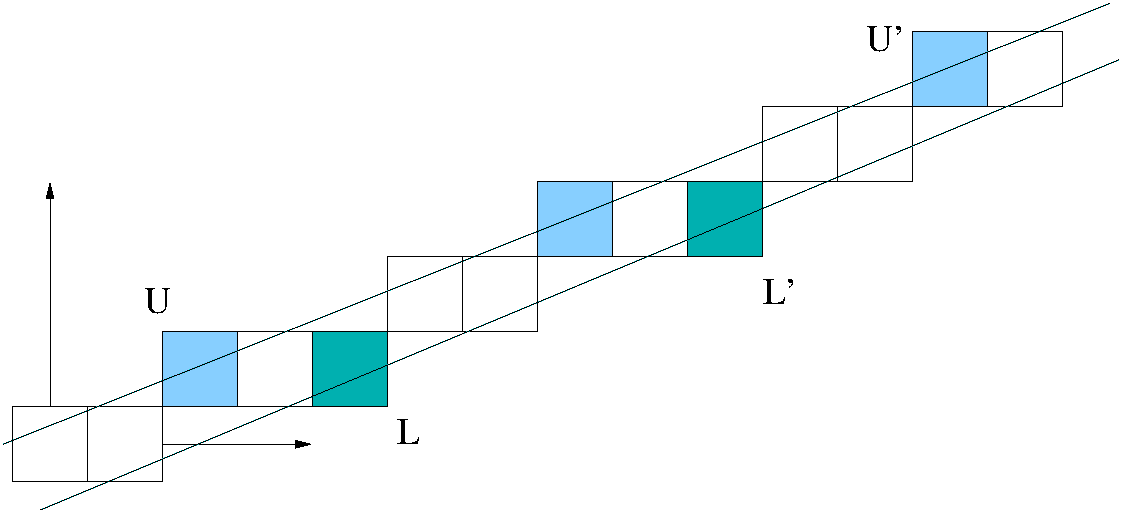
\includegraphics[width=7cm]{UU_LL}
    \caption{Description des notations : $U$ et $U'$ sont les points
      d'appui sup�rieurs d'abscisses  minimale et maximale, $L$ et $L'$
      sont les  points   d'appui  inf�rieurs d'abscisses  minimale   et
      maximale.}
    \label{fig:UULL}
  \end{center}
\end{figure}

L'algorithme de reconnaissance de \citeauthor{debledthese}   consid�re
l'ajout    d'un  point $M(x,y)$  de    reste $r=ax-by$ au segment d�j�
reconnu. Cet algorithme repose sur le th�or�me suivant~:

\begin{theo}[\cite{debledthese}]
�tant  donn� l'ajout d'un  point $M$ de  reste $r=ax-by$ � droite d'un
segment d�j� reconnu $\Sigma$, et les points d'appui $U$, $U'$, $L$ et
$L'$, nous avons~:
\begin{itemize}
\item si $\mu\leq r < \mu+b$ alors $M$ appartient � la droite
$\mathcal{D}(a,b,\mu)$ et donc $\Sigma\cup M$ est un segment discret
\item si $r>\mu+b$ ou $r<\mu-1$ alors $\Sigma\cup M$ n'est pas un
segment de droite discr�te
\item si $r=\mu-1$ alors $M$ est faiblement ext�rieur � la droite
discr�te $\mathcal{D}$ et donc $\Sigma\cup M$ est un segment de droite discr�te dont
la pente est donn�e par le vecteur $\overrightarrow{UM}$
\item si $r=\mu+b$ alors $M$ est faiblement ext�rieur � $\mathcal{D}$
et donc $\Sigma\cup M$ est un segment de droite discr�te dont la pente
est donn�e par $\overrightarrow{LM}$
\end{itemize}
\end{theo}

Si l'ajout se fait � gauche du segment $\Sigma$, il suffit de
consid�rer les vecteurs $\overrightarrow{U'M}$ et $\overrightarrow{L'M}$ au lieu de
$\overrightarrow{UM}$ et $\overrightarrow{LM}$.

La clef de ce th�or�me est la suivante~: si nous ajoutons un point
faiblement ext�rieur � un segment,  nous devons modifier les
param�tres de la droite reconnue tout en garantissant que tous les points
de $\Sigma$ d�j� reconnus appartiennent aussi � cette nouvelle droite
discr�te.

D'une mani�re plus pr�cise, si $(b,a)$ d�signe le vecteur directeur de
la droite contenant $\Sigma$, l'ajout d'un point faiblement ext�rieur
introduira le vecteur $(b',a')$. Or, $M$ etant faiblement ext�rieur,
les vecteurs $(b,a)$ et $(b',a')$ sont uni-modulaires, c'est-�-dire
que nous avons :
\begin{displaymath}
ab'-ba'=1
\end{displaymath}
Pour conclure cette preuve, \citeauthor{debledthese} utilise le
th�or�me de \aut{Minkowski} qui stipule qu'il n'y a pas de points entiers
dans le parall�logramme d�fini par des vecteurs uni-modulaires (voir \citep{hardy}). Nous
reprenons une illustration de \citeauthor{vialardthese} pour
repr�senter les diff�rents cas de ce th�or�me (voir figure
\ref{fig:algo_debled}).
\begin{figure}[htbp]
  \begin{center}
    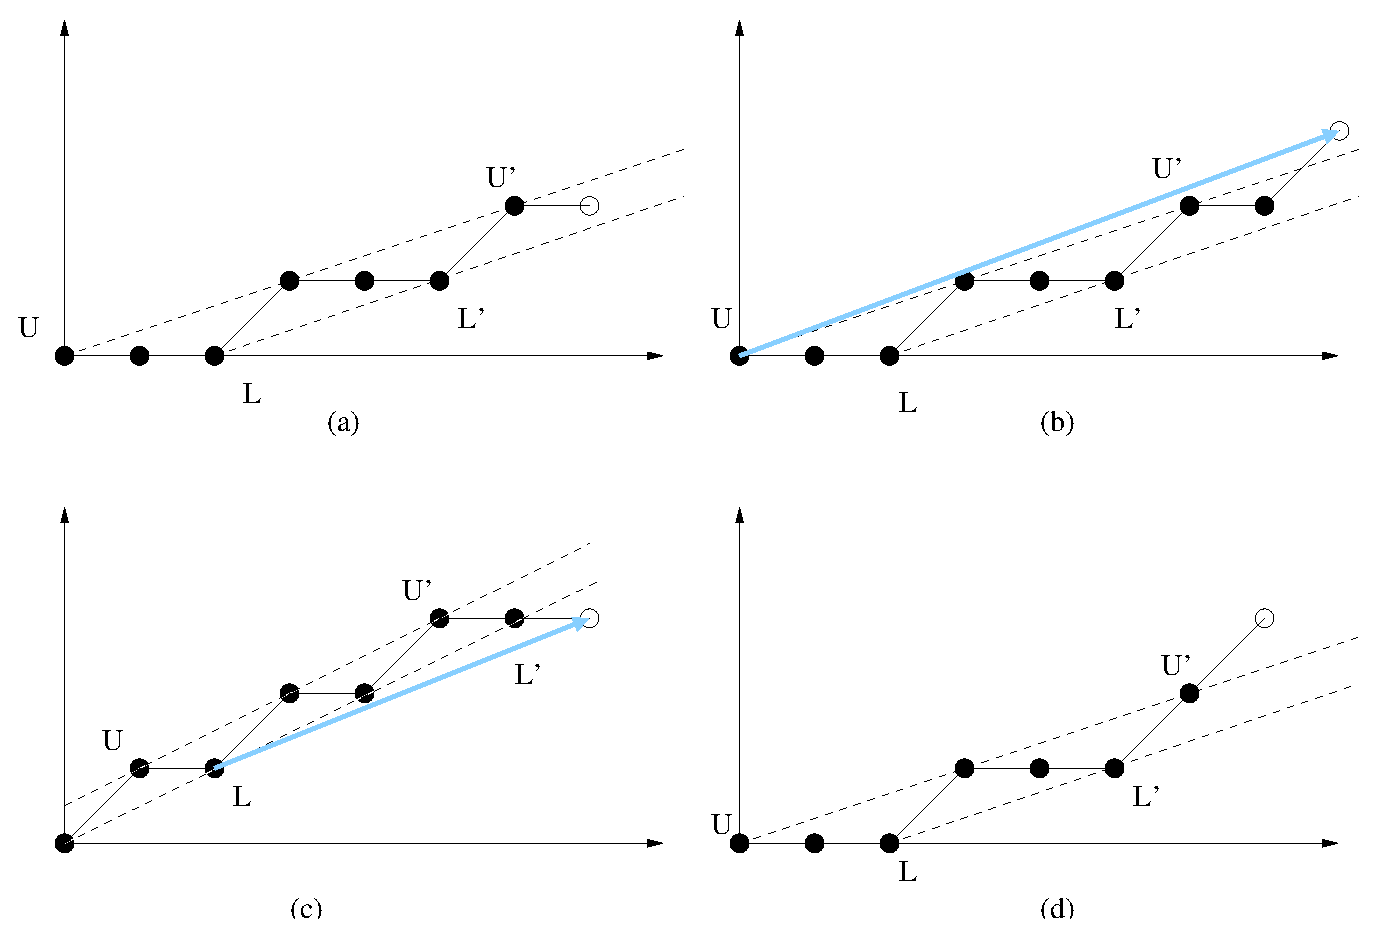
\includegraphics[width=13cm]{algo_debled}
    \caption[Diff�rents cas de figure lrsde l'ajout d'un point � une
      droite  discr�te]{Diff�rents cas de figure  lors de l'ajout d'un
      point  �  une droite   discr�te~:  $(a)$  ajout d'un    point ne
      changeant pas les param�tres,  $(b)$ ajout d'un point faiblement
      ext�rieur sup�rieur, dans ce cas   le vecteur clair indique  les
      nouveaux param�tres du  segment discret, $(c)$  ajout d'un point
      faiblement   ext�rieur  inf�rieur,  le   vecteur  clair  indique
      toujours le nouveau param�trage de la courbe et $(d)$ ajout d'un
      point    fortement   ext�rieur    et mise     en    �chec  de la
      reconnaissance.}
    \label{fig:algo_debled}
  \end{center}
\end{figure}

Nous  pouvons  maintenant d�crire   l'algorithme de  reconnaissance de
droite   discr�te      de    \cite{debledthese}      (voir  algorithme
\ref{alg:debled}).   Cet   algorithme  correspond �  une  modification
apport�e    par     \cite{vialardthese,vialard_GMIP} �    l'algorithme initial  de
\citeauthor{debledthese}.


\begin{algorithm}[!htbp]
\caption{Algorithme de reconnaissance de droite discr�te de \cite{debledthese}}
\label{alg:debled}
\begin{algorithmic}[1]
\EXTERNNAME \INTERNNAME{Reconnaissance\_Debled($\mathcal{S}$)} 
\COMMENT{Algorithme modifi� par \cite{vialardthese}}
\STATE $M(x,y)$ et $M'(x',y')$ sont les deux premiers points de $\mathcal{S}$
\STATE $a=y'$, $b=1$ et $\mu=0$
\STATE $U=L=(0,0)$
\STATE $U'=L'=(1,y')$
\STATE SEGMENT=Vrai
\WHILE{$\mathcal{S}$ n'a pas �t� compl�tement parcouru et SEGMENT}
\STATE $M(x,y)$ = point suivant dans $\mathcal{S}$
\STATE $r=ax-by$
\IF{$r<\mu-1$ ou $r>\mu+b$}
\STATE SEGMENT=Faux
\ELSE
\IF{$r=\mu-1$ ou $r=\mu+b$}
\IF{$r=\mu-1$}
\STATE $L=L'$
\STATE $U'=M$
\STATE $a=y-y_U$
\STATE $b=x-x_U$
\STATE $\mu=ax-by$
\ENDIF
\IF{$r=\mu+b$}
\STATE $U=U'$
\STATE $L'=M$
\STATE $a=y-y_L$
\STATE $b=x-x_L$
\STATE $\mu=ax-by-b+1$
\ENDIF
\ELSE
\IF{$r=\mu$}
\STATE $U'=M$
\ELSIF{$r=\mu+b-1$}
\STATE $L'=M$
\ENDIF

\ENDIF
\ENDIF
\ENDWHILE
\end{algorithmic}
\end{algorithm}
Cet algorithme est non  seulement lin�aire en  le nombre de  pixels de
$\mathcal{S}$ et  optimal  en   m�moire,  mais  il offre   aussi   une
possibilit� d'impl�mentation tr�s rapide.

En se basant sur une analyse  identique, \cite{debledthese} propose aussi  des
algorithmes de reconnaissance de droites discr�tes {\it �paisses} dans
lesquelles les  droites  discr�tes standards (4-connexes) sont  un cas
particulier.   Dans    ce   cas   pr�cis    des   droites   standards,
\cite{vialardthese}    a   illustr�   un    passage direct    entre la
reconnaissance d'une  droite  4-connexe   et la  reconnaissance  d'une
droite na�ve (8-connexe)~:

\begin{prop}[\cite{vialardthese}]
Soient  $a$, $b$  et  $\mu$ dans  $\Z$  avec  $0\leq a<b$, le  code de
\aut{Freeman}       4-connexe     de    la    droite   discr�te     standard
$\mathcal{D}(a,b-a,\mu)$ est identique au code de \aut{Freeman} 8-connexe de
la droite discr�te na�ve $\mathcal{D}(a,b,\mu)$.
\end{prop}

Gr�ce � cette propri�t�,  les algorithmes de reconnaissance de droites
discr�tes    standards  s'obtiennent   �   partir  des  algorithmes de
reconnaissance des droites  discr�tes na�ves par une simple r��criture
dans le code de \aut{Freeman}.

\subsubsection{Comparaisons entre approche arithm�tique et approche duale}
\label{sec:comp-dual-arith}

Pour terminer cette analyse,    nous   montrons les liens entre     la
repr�sentation d'une droite par son domaine des solutions dans le dual
et la repr�sentation sous forme arithm�tique.   Dans un premier temps,
nous caract�risons   dans l'espace primal,  les diff�rents  sommets et
ar�tes  du domaine associ�  �  un segment discret   dans le dual (voir
\citealt{Smeulders84,bruck93,vittone}).

Nous consid�rons une   cellule de Farey dont   les sommets sont  not�s
$(ABCD)$ comme indiqu� dans la  figure \ref{fig:coupure_ilroy}.  �tant
donn�    un   segment    de     droite     discr�te   de     param�tre
$\mathcal{D}(a,b,\mu)$, nous  avons  alors les  propri�t�s (illustr�es
figure \ref{fig:dual_arith})~:
\begin{prop}
\ 

\begin{itemize}
\item La transform�e de $D$ dans l'espace primal est la droite d'appui
 sup�rieure associ�e au segment discret. $D$ a pour coordonn�es
$(\frac{a}{b},\frac{\mu}{b})$.
\item La transform�e de $B$ dans l'espace primal est la droite d'appui
  inf�rieure, translat\'ee de 1 en $y$, associ�e au segment discret. $B$
a pour coordonn�es $(\frac{a}{b},\frac{\mu+1}{b})$.
\item  La droite $(AD)$ (resp. $(DC)$) correspond au point d'appui
sup�rieur d'abscisse maximale $U'$ (resp. minimale $U$).
\item La droite $(AB)$ (resp. $(BC)$) correspond au point d'appui
inf�rieur, translat\'e de 1 en $y$, d'abscisse minimale  $L$ (resp. maximale $L'$).
\item Le sommet $A$ correspond dans le primal � la droite passant par
$U'$ et le translat\'e de $L$ de 1 en $y$.
\item Le sommet $C$ correspond dans le primal � la droite  passant par
$U$ et le translat\'e de $L'$ de 1 en $y$.
\end{itemize}
\end{prop}


\begin{figure}[htbp]
  \begin{center}
    \subfigure[]{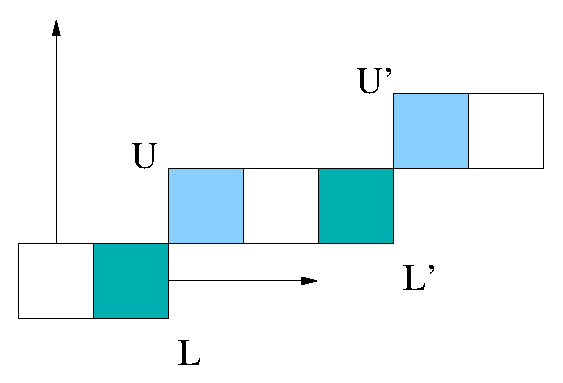
\includegraphics[width=3.5cm]{dual_arith}}
    \subfigure[]{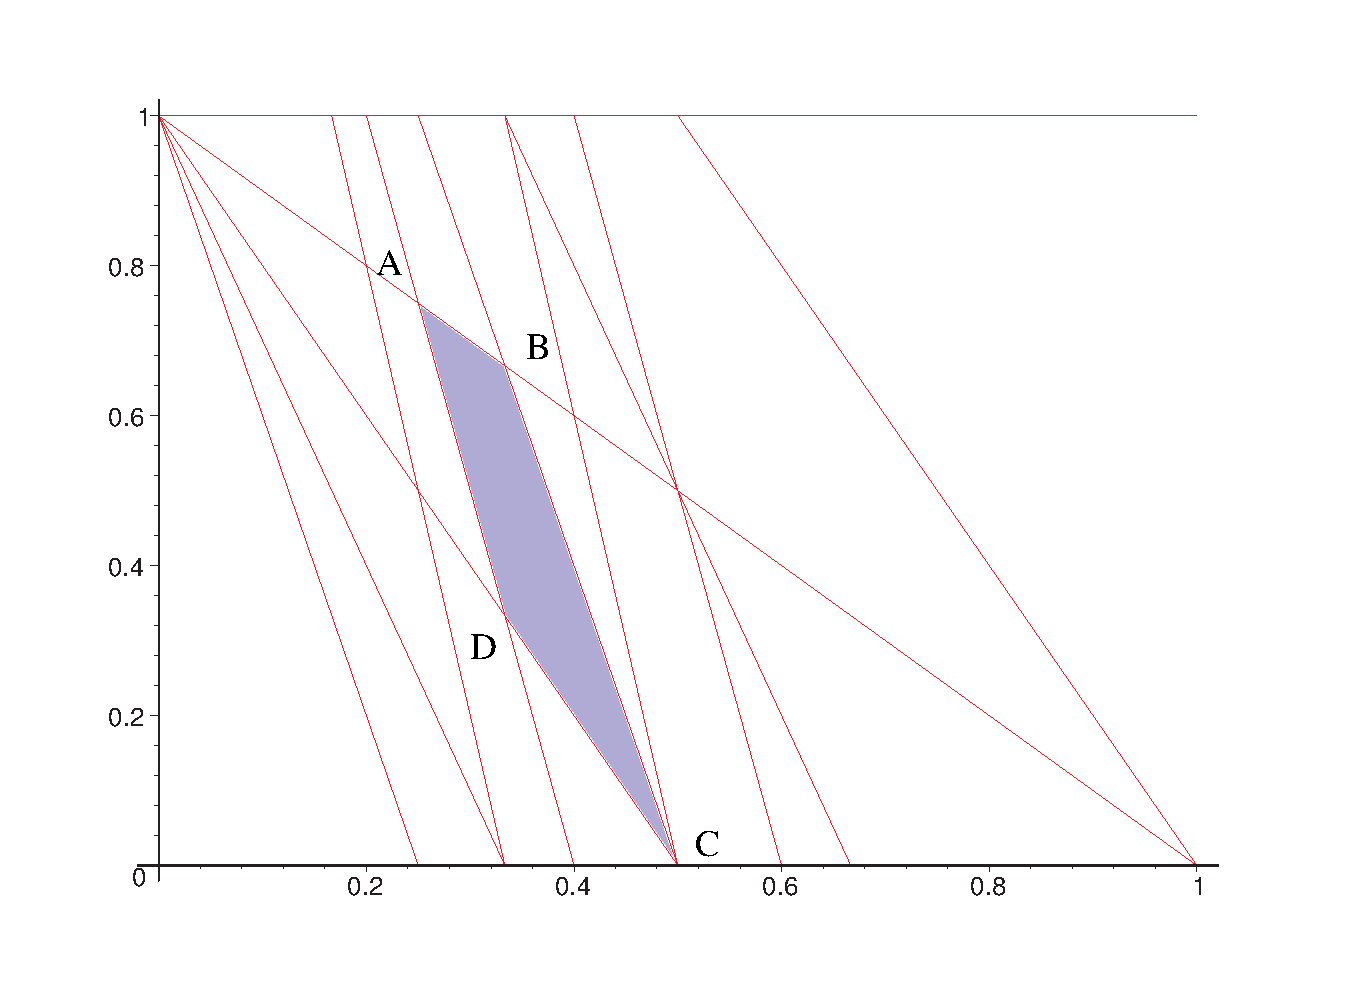
\includegraphics[width=7.5cm]{dual_droite2}}
    \subfigure[]{\includegraphics[width=8cm]{dual_arith2}}
    \caption[Comparaisons entre approche arithm�tique et approche
bas�e   sur l'espace  des   droites  dans le dual]{Comparaisons  entre
approche arithm�tique et approche bas�e sur  l'espace des droites dans
le  dual~: $(a)$ segment  de droite arithm�tique $\mathcal{D}(1,3,1)$,
$(b)$ cellule de  Farey associ�e au segment  discret dans l'espace des
param�tres et $(c)$  repr�sentation dans l'espace primal des  �l�ments
caract�ristiques    dans  le  dual,  la partie    claire  correspond �
l'ensemble  des orientations des  droites r�elles se discr�tisant dans le
segment discret.}
    \label{fig:dual_arith}
  \end{center}
\end{figure}


Gr�ce � ces propri�t�s, nous pouvons construire enti�rement la cellule
de Farey associ�e � un segment discret �  partir de sa caract�risation
arithm�tique.   R�ciproquement, � partir de   la cellule de Farey nous
pouvons  obtenir   les   param�tres  minimaux $a$   et $b$   tels  que
$pgcd(a,b)=1$ et le param�tre de  translation $\mu$ caract�risant  les
droites discr�tes.


\subsubsection{Bilan des algorithmes de reconnaissance pr�sent�s}

Dans des  utilisations pratiques de  ces algorithmes de reconnaissance
de  droite   discr�te, le choix    d'un algorithme  peut  ne pas  �tre
�vident. Dans  le tableau \ref{table:approche_prog} nous  r�sumons les
diff�rentes techniques pr�sent�es avec leur analyse en complexit� et
hypoth�ses.


\begin{sidewaystable}[htbp]
%\begin{table}[htbp]
\begin{tabular}{|p{4.5cm}|p{2cm}|p{3cm}|c|c|p{4cm}|}
\hline
 Algorithme & Complexit� en temps & Incr�mental  & M�moire & Hypoth�ses & Remarques\\
\hline
 \cite{megiddo} & $O(n)$ & oui, voir \cite{buzer}&- & Aucune & lin�arit� uniquement\\
\hline
 \cite{P16} & $O(nlog(n))$& oui & $O(n^2)$& Aucune& \\
\hline
\cite{vittonethese} & $O(n^3log(n))$& oui & $O(n^2) $& Aucune&
coordonn�es sous forme irr�ductible \\
\hline
\citeauthor{vittonethese} modifi� (alg. \ref{alg:vittonebis})&
$O(nlog^2(n))$& oui & $O(n^2) $& Aucune&
coordonn�es sous forme irr�ductible  \\
\hline
\cite{rourke} & $O(n)$& oui & $O(n)$ & pixels tri�s selon un
axe& \\
\hline
\cite{dor91,bruck93} & $O(n)$ & oui en $O(1)$ par
ajout & $O(1)$ & connexit�&coordonn�es
sous forme irr�ductible\\
\hline
\cite{debledthese} & $O(n)$ & oui en $O(1)$ par ajout &
$O(1)$ & connexit�&caract�risation arithm�tique\\
\hline
\end{tabular}
\caption{Algorithmes et complexit�s pour la reconnaissance de droites discr�tes.}
\label{table:approche_prog}
\end{sidewaystable}
%\end{table}

\subsubsection{De la reconnaissance � la segmentation de courbe}
\label{sec:de-la-reconnaissance}

Comme nous l'avons illustr� dans le  tableau \ref{tab:oct}, le passage
d'une droite discr�te dans  le premier octant  vers les autres octants
s'op�re par sym�tries  d'axes.  Cependant, dans un  contexte  g�n�ral,
nous avons un ensemble de pixels $\mathcal{E}$ sur lequel nous n'avons
aucune information quant � l'octant auquel il appartient, le processus
de reconnaissance ne peut donc s'appliquer directement.


Nous consid�rons un ensemble  de pixels $\mathcal{E}$ et  nous voulons
savoir quel est le   plus long segment   de droite discr�te qu'il  est
possible de reconna�tre � partir d'un  pixel $M$ de $\mathcal{E}$, dans
une direction donn�e. L'id�e pour r�soudre  ce probl�me se d�compose en  deux
�tapes~:
\begin{enumerate}
\item � partir de $M$, d�tecter dans quel octant se trouve le morceau
de courbe de $\mathcal{E}$~;
\item    une fois   l'octant   connu,  on    utilise   le processus de
reconnaissance de droite discr�te dans le premier octant et le tableau
des sym�tries \ref{tab:oct}.
\end{enumerate}

A partir d'un point, calculer dans quel octant se trouve un morceau de
courbe de    $\mathcal{E}$ localement en $M$   se   fait simplement en
regardant le code de \aut{Freeman}. D�s que nous  avons rep�r� dans ce
codage deux codes distincts cons�cutifs, nous  savons dans quel octant
se trouve la courbe en partant de $M$.   M�me si ce calcul est trivial
sur  le   plan th�orique, l'impl�mentation   en   temps optimal de  ce
processus n'est  pas �vident.  Pour  cela, \cite{DEB95} ont propos� un
algorithme pour le probl�me plus g�n�ral de  la segmentation de courbe
en droites discr�tes arithm�tiques en temps optimal en impl�mentant ce
processus   de d�couverte  d'octant  en m�me  temps  que  celui  de la
reconnaissance.

Le    processus de    segmentation    consid�re une  courbe   discr�te
$\mathcal{E}$, un  point   de d�part et un   sens  de parcours.   Elle
construit la   segmentation de  cette courbe   en  morceaux de droites
discr�tes de longueurs maximales. Ainsi, en partant d'un point $M$, on
va  reconna�tre   le  plus  grand   morceau  de   droite  discr�te  de
$\mathcal{E}$. Une fois  la reconnaissance termin�e, on initialise  un
nouveau  processus de reconnaissance �   partir  du premier point  non
reconnu  (voir  figure  \ref{fig:segmentation}).  Cette   segmentation
permet  une  description  polygonale  de la   courbe discr�te  tout en
conservant des propri�t�s    de r�versibilit�~: on  peut  trivialement
reconstruire l'ensemble $\mathcal{E}$ �  partir de sa segmentation  en
segments discrets.

\begin{figure}
  \begin{center}
    \subfigure[]{\includegraphics[width=4.2cm]{cercle_segm}}
    \subfigure[]{\includegraphics[width=4.2cm]{carre_segm}}
    \subfigure[]{\includegraphics[width=4.2cm]{sinc_segm}}
    \caption[Exemples de segmentation d'une courbe discr�te en droite
    discr�te avec     l'algorithme    de   \cite{DEB95}]{Exemples   de
    segmentation  d'une   courbe discr�te  en   droites discr�tes avec
    l'algorithme  de  \cite{DEB95}~:    la courbe   polygonale   noire
    correspond au r�sultat de la segmentation  et la fl�che indique le
    point  d�part,  $(a)$ un cercle discret,  $(b)$  un carr� avec une
    rotation de  10 degr�s et $(c)$  sur une courbe  construite par
    une fonction     sinus cardinale.}
    \label{fig:segmentation}
  \end{center}
\end{figure}



Nous verrons au    chapitre \ref{chap-mesuresa} l'utilisation de   cet
outil pour l'estimation de la longueur d'une courbe discr�te.

%%%%%%%%%%%%%%%%%%%%%%%%%%%%%%%%%%%%%%%%%%%%%%%%%%%%%%%%%%%%%%%
\section{Droites discr{\`e}tes 3D}
\label{sec:droites-discretes-3d}

Nous regardons maintenant  la construction    et les propri�t�s    des
droites discr�tes tridimensionnelles. La synth�se et la reconnaissance
de ces objets   sont utilis�es dans  de  tr�s nombreuses applications.
Par exemple,  dans  le contexte de  la  synth�se d'image par  lanc� de
rayons, la  construction de rayons discrets  3D a permis l'acc�l�ration
de nombreuses techniques.
 
Nous commen�ons  par  pr�senter  les diff�rentes  approches existantes
pour  le  trac�  de droites discr�tes   3D.  Puis  nous pr�sentons les
propri�t�s  de ces droites ainsi que  les  algorithmes permettant leur
reconnaissance.

\subsection{Caract�risation et propri�t�s des droites discr�tes 3D}

Comme nous l'avons pr�sent� pr�c�demment, le trac� de droites dans des
grilles 3D  a �t�  tr�s  d�velopp� dans  le    cadre de la  synth�se
d'images  par   lanc� de  rayons  \citep{AMA87,KAU87b,VID92,Salam}.  Le
probl�me s'�crit en ces termes~: �tant donn�  deux points d'une grille
dans $\Z^3$, comment tracer la droite joignant ces deux points.

Pour r�soudre ce probl�me, deux approches sont possibles.
\begin{description}
\item[Le trac�  par projection]   consiste  en une   d�composition  du
probl�me  en dimension 2.  Ainsi,  le principe consiste  � tracer deux
droites discr�tes  2D  dans deux  plans canoniques  de la  grille pour
ensuite construire la droite 3D par projection inverse \citep{AMA87}.
\item[Le trac�   direct]  consiste en un  trac�   de la  droite  en 3D
directement. Ces   approches se basent sur   une g�n�ralisation 3D des
algorithmes 2D    classiques    comme  celui     de    \aut{Bresenham}
\citep{KAU86,CO91}.
\end{description}

Sur le plan de la caract�risation  de tels objets, de nombreux auteurs
ont  propos�    des d�finitions   de droites    discr�tes  26-connexes
\citep{KIM83,STO91}.  Dans     cette   partie,   nous   pr�sentons  la
caract�risation   arithm�tique  de   ces    droites   propos�es    par
\cite{debledthese}   et reprise par    \cite{3Dnss}  dans le cadre  de
l'estimation de longueur d'une   courbe 3D par segmentation  en droite
discr�te.

Nous   consid�rons  la droite  discr�te    3D   de vecteur   directeur
$(a,b,c)^T\in\Z^3$  appartenant  dans le  premier  $48\eme$ d'espace,
c'est-�-dire tel que  $a\geq  b\geq  c>0$.  Nous discuterons dans   la
section suivante la g�n�ralisation � tout l'espace.

\begin{defi}[Droite discr�te 3D \citep{debledthese}]
\label{def:droite3D}
  La      droite         discr�te                   3D,          not�e
  $\mathcal{D}_{3D}(a,b,c,\mu,\mu',e,e')$,  dont le vecteur  directeur
  $V(a,b,c)$ est dans le premier $48\eme$ d'espace, est d�finie comme
  �tant l'ensemble  des   voxels $(x,y,z)$  de   $\Z^3$  v�rifiant  les
  in�quations diophantiennes suivantes~:
  \begin{displaymath}
    \mathcal{D} \left \{ 
      \begin{array}{c}
        \mu \leq cx -az<\mu+e\\
        \mu'\leq bx -ay<\mu'+e'\\
      \end{array}
    \right .
 \end{displaymath}
avec $\mu$, $\mu'$, $e$ et $e'$ dans $\Z$. $\mu$ et $\mu'$ sont les
{\bf bornes inf�rieures} de $\mathcal{D}_{3D}$, $e$ et $e'$ repr�sentent
{\bf l'�paisseur arithm�tique} de $\mathcal{D}_{3D}$. 
\end{defi}
Une    d�finition  arithm�tique    plus   g�n�rale  a    �t�  propos�e
par
\cite{figueiredo}.



Comme  nous  pouvons   le    remarquer,   la projection    la   droite
$\mathcal{D}_{3D}$ sur le plan  $Oxz$ correspond � la  droite discr�te
2D $\mathcal{D}(c,a,\mu,e)$. De   la  m�me mani�re, la  projection  de
cette  droite 3D  sur   le  plan $Oxy$   correspond  �  la   droite 2D
$\mathcal{D}(b,a,\mu',e')$.


Nous d�finissons les droites      discr�tes na�ves 3D de  la     fa�on
suivante~:

\begin{defi}[Droite discr�te na�ve 3D \citep{debledthese}]
  une        droite   discr�te             3D          de   param�tres
  $\mathcal{D}_{3D}(a,b,c,\mu,\mu',e,e')$  dans  le  premier $48\eme$
  d'espace est dite {\bf na�ve} si et seulement si l'�paisseur v�rifie
  $e=e'=a$.
\end{defi}


D'apr�s la remarque pr�c�dente, la droite 3D se projette bijectivement
sur les plans $Oxy$  et $Oxz$ en deux   droites na�ves 2D.  Par
cons�quence,  de la m�me  mani�re qu'en 2D, nous  avons un th�or�me de
structure  des  droites  discr�tes   3D  en  fonction  de  l'�paisseur
arithm�tique~:

\begin{theo}[connexit� des droites discr�tes 3D \citep{debledthese}]
\label{theo_struct3D}
  Consid�rons une droite discr�te
  $\mathcal{D}_{3D}(a,b,c,\mu,\mu',e,e')$ avec $a>b>c>0$, alors
  \begin{itemize}
  \item si $e \geq a + c$ et $ e' \geq a + b $, $\mathcal{D}_{3D}$ est
    6-connexe  (voir figure \ref{fig:droite3D6con}).
  \item si $e \geq a + c$ et $ a \leq  e' < a + b $, ou $ e' \geq a + b$ et
    $a \leq  e  < a + c $,  $\mathcal{D}_{3D}$ est 18-connexe
  \item si $a \leq  e  < a + c $ et  $ a \leq  e' < a + b $,
    $\mathcal{D}_{3D}$ est 26-connexe (voir figure \ref{fig:droite3D26con}.)
  \item si $ e < a$ ou $e'< a$,  $\mathcal{D}_{3D}$ est d�connect�e.
  \end{itemize}
\end{theo}

La preuve de ce th�or�me se base sur une analyse des projections de la
droite 3D et sur le th�or�me \ref{theo:struct2D} de connexit� des droites discr�tes 2D
 \citep{debledthese}.


\begin{figure}[htbp]
  \centering
  \includegraphics[width=8cm]{pd61}
  \caption{Droites discr�tes 3D de param�tres
    $\mathcal{D}_{3D}(10,7,3,0,-9,13,17)$,  conform�ment au   th�or�me
    \ref{theo_struct3D},   cette  droite est  6-connexe.  De plus, les
    droites  2D  dans   les  plans  $Oxy$  et  $Oxz$  sont  4-connexes
    \citep{debledthese}.}
  \label{fig:droite3D6con}
\end{figure}

\begin{figure}[htbp]
  \centering
  \subfigure[]{\includegraphics[width=6cm]{pd262}}
  \subfigure[]{\includegraphics[width=6cm]{pd263}}
  \caption[Droites discr�tes 3D 26-connexes]{Droites discr�tes 3D 26-connexes~: $(a)$ droite na�ve
    $\mathcal{D}_{3D}(10,7,3,0,0)$ et  $(b)$ droite na�ve  
    $\mathcal{D}_{3D}(10,7,3,-5,0)$ \citep{debledthese}.}
  \label{fig:droite3D26con}
\end{figure}




%Nous pouvons faire un lien entre les discr�tisations standards et la droite discr�te
%3D avec le th�or�me suivant~:

%\begin{theo}[\cite{3Dnss}]
%  La discr�tisation GIQ (Grid Intersect Quantization) d'une droite
%  r�elle 3D est une discr�te na�ve 3D.
%\end{theo}

%\begin{mapreuve}
%  Sans perte de g�n�ralit�, nous consid�rons  $\mathcal{D}_{euc}$ une
%  droite r�elle  3D de vecteur directeur  $(a,b,c)\in\mathbb{Z}^3$
%  avec $a\geq b\geq c>0$, d�finie par~:
%\begin{displaymath}%$$
%\begin{array}{cc}
%\mathcal{D}_{euc} = &
%\left\{
%  \begin{array}{l}
%    z = \frac{cx - r}{a}\\
%\ \\
%    y = \frac{bx - r'}{a}\\
%   \end{array}
%\right.
%\end{array}
%\end{displaymath}
%                            %$$

%Nous consid�rons aussi les plans euclidiens $\mathcal{P}_1: z=\frac{cx - r}{a}$
%et  $\mathcal{P}_2: y=\frac{bx - r'}{a}$. La discr�tisation GIQ de ces
%plans nous donne les plans discrets na�fs suivants (voir paragraphe \ref{sec:plans-discrets})~:
%\begin{displaymath}
%\begin{array}{l}
%GIQ(\mathcal{P}_1) = \mathcal{P}(c,0,-a,r+\left[ \frac{a}{2} \right])\\
%GIQ(\mathcal{P}_2) = \mathcal{P}(b,-a,0,r'+\left[ \frac{a}{2} \right])\\
%\end{array}
%\end{displaymath}

%o�  $\mathcal{P}(u,v,w,\mu) : \mu \leq ux+vy+wz < \mu+
%max(|u|,|v|,|w|)$ \citep{AND,DEBBOS94}.

%Par la suite,  nous consid�rons une  discr�tisation GIQ sans ambigu�t�
%(voir \citep{jonas97}).   Plus formellement,  une  ambigu�t� (ou  {\it
%bulles}  dans  l'approche d'\citeauthor{andres_standard}  du paragraphe
%\ref{sec:discr-de-simpl})  correspond  � une  intersection   entre  la
%courbe et  la grille �  �quidistance entre deux pixels. Nous supposons
%en fait une strat�gie globale pour enlever les cas pathologiques.

%D'apr�s la d�finition \ref{def:droite3D} et le th�or�me de structure
%\ref{theo_struct3D}, l'intersection entre ces deux plans naifs d�finie
%la droite discr�te na�ve 26-connexe~:
%\begin{displaymath}
%\begin{array}{cc}
%\mathcal{D}_{3D} = &
%\left\{
%  \begin{array}{l}
%    r+\left[ \frac{a}{2}\right] \leq cx-az < r+\left[ \frac{a}{2}\right] + a\\
%    r'+\left[ \frac{a}{2}\right] \leq bx-ay < r'+\left[ \frac{a}{2}\right] +a
%   \end{array}
%\right.
%\end{array}
%\end{displaymath}%$$


%L'objectif maintenant est de montrer que $\mathcal{D}_{3D} $ co�ncide
%avec $GIQ(\mathcal{D}_{euc})$. Pour cela, supposons un voxel $v$ de
%$\mathcal{D}_{3D}$, nous avons alors ($dist$ repr�sente la distance
%euclidienne)~:

%\begin{displaymath}
%dist(v,\mathcal{P}_1) \leq \sqrt{2}\text{ et }dist(v,\mathcal{P}_2) \leq \sqrt{2}
%~\Rightarrow ~dist(v,\mathcal{D}_{euc}) \leq \sqrt{2}
%\end{displaymath}%$$

%\noindent Ce qui est �quivalent �~:
%\begin{displaymath}
%v\in\mathcal{D} \Rightarrow v\in GIQ(\mathcal{D}_{euc})
%\end{displaymath}
%Nous avons donc~:
%\begin{displaymath}
%\mathcal{D} \subset GIQ(\mathcal{D}_{euc})
%\end{displaymath}

%Pour prouver l'inclusion inverse, nous consid�rons    $v'\in GIQ(\mathcal{D}_{euc})$,  si
%$v'\not\in\mathcal{D}$, nous avons deux possibilit�s~:
%\begin{itemize}
%\item $dist(v',\mathcal{P}_1)>\sqrt{2}$ ou $dist(v',\mathcal{P}_2)>\sqrt{2}$
%  ce qui est �quivalent �
%  $dist(v',\mathcal{D}_{euc})>\sqrt{2}$ ce qui implique une contradiction
%  avec la discr�tisation GIQ de   $\mathcal{D}_{euc}$ ;
%\item $dist(v',\mathcal{D}_{euc})\leq\sqrt{2}$ mais �tant donn� que le
%  processus est sans ambiguit�,  $v'$ d�connecte $\mathcal{D}$ ce qui
%  est en contradiction avec le th�or�me de structure \ref{theo_struct3D}.
%\end{itemize}
%Nous obtenons finalement~:
%\begin{displaymath}
%\mathcal{D}=GIQ(\mathcal{D}_{euc})
%\end{displaymath}
%\end{mapreuve}



\subsection{Trac� de droites discr�tes 3D}

Nous d�taillons  ici  les diff�rents algorithmes  de  trac�  de droite
discr�te  na�ve  3D.   Nous pr�sentons  tout  d'abord  l'algorithme de
\cite{CO91} qui correspond �  une g�n�ralisation  tridimensionnelle de
l'algorithme  de      \cite{bres65}            (voir        algorithme
\ref{alg:cohen3D}). Ceux-ci consid�rent deux voxels   de la grille   et
tracent le segment de droite 26-connexe les joignant.

\begin{algorithm}[htbp]
\caption{Trac� de droites discr�tes 3D de \cite{CO91}}
\label{alg:cohen3D}
\begin{algorithmic}[1]
\EXTERNNAME \INTERNNAME{Trac�\_3D\_Cohen\_Kaufman($A$,$B$)}
\\ \COMMENT{avec $A,~B\in\Z^3$ tels que $x_B-x_A>0$, $y_B-y_A>0$ et $z_B-z_A>0$}
\STATE ${v_{x}=x_{B}-x_{A}}$, ${v_{y}=y_{B}-y_{A}}$, ${v_{z}=z_{B}-z_{A}}$;
\STATE $s_x=sgn(v_x)$, $s_y=sgn(v_y)$,  $s_z=sgn(v_z)$
\STATE $a_x=abs(v_x)$, $a_y=abs(v_y)$, $a_z=abs(v_z)$
\STATE $b_x=2a_x$, $b_y=2a_y$,  $b_z=2a_z$
\STATE $e_{xy}=a_y-a_x$, $e_{xz}=a_z-a_x$ , $e_{zy}=a_y-a_z$ 
\STATE ${x=x_{A}}$, ${y=y_{A}}$, ${z=z_{A}}$ 
\STATE $n=a_x+a_y+a_z$
\WHILE{$n\neq 0$}
\STATE $n-=1$
\STATE  Affiche\_point$(x,y,z)$
\IF{$e_{xy}<0$}
\IF{$e_{xz}<0$}
\STATE $x+=s_x$
\STATE $e_{xy}+=b_y$, $e_{xz}+=b_z$
\ELSE
\STATE $z+=s_z$
\STATE  $e_{zy}+=b_y$, $e_{xz}-=b_x$
\ELSIF{$e_{zy}<0$}
\STATE $z+=s_z$
\STATE $e_{zy}+=b_y$, $e_{xz}-=b_x$
\ELSE
\STATE $y+=s_y$
\STATE $e_{xy}-=b_x$, $e_{zy}-=b_z$
\ENDIF
\ENDIF
\ENDWHILE
\end{algorithmic}
\end{algorithm}

En se basant sur la caract�risation arithm�tique, nous pr�sentons l'algorithme
de    trac�   propos�  par     \cite{debledthese}  (voir    algorithme
\ref{alg:debled3D}). Ce trac� consid�re deux param�tres suppl�mentaires
que sont  les  bornes  inf�rieures  $\mu$  et  $\mu'$.  Ainsi,  si nous
consid�rons    $\mu=\mu'=-\left   [      \frac{max(|vx|,|vy|,|vz|)}{2}
\right]+1$, nous nous ramenons au trac�  de \cite{bres65} �tendu en 3D
par \cite{CO91}.


\begin{algorithm}[htbp]
\caption{Trac� de droites discr�tes 3D de \cite{debledthese}}
\label{alg:debled3D}
\begin{algorithmic}[1]
\EXTERNNAME \INTERNNAME{Trac�\_3D\_Debled($A$,$B$,$\mu$,$\mu'$)}
\\ \COMMENT{avec $A,~B\in\Z^3$ tels que $x_B-x_A>y_B-y_A>0$ et $y_B-y_A>z_B-z_A>0$}
\STATE ${v_{x}=x_{B}-x_{A}}$, ${v_{y}=y_{B}-y_{A}}$,
${v_{z}=z_{B}-z_{A}}$
\STATE ${r_{1}=v_{z}*x_{A} - v_{x}*z_{A} - \mu}$
\STATE ${r_{2}=v_{y}*x_{A} - v_{x}*y_{A} - \mu'}$
\STATE ${x=x_{A}}$, ${y=y_{A}}$, ${z=z_{A}}$ 
\WHILE{${x <x_{B}} $}
\STATE ${x = x+1}$
\STATE ${r_{1}=r_{1}+v_{z}}$ 
\STATE  ${r_{2}=r_{2}+v_{y}}$ 
\IF{${r_{1}<0}$ ou ${r_{1}\geq v_{x}}$}
\STATE ${z = z+ 1}$
\STATE ${r_{1} = r_{1} - v_{x}}$
\ENDIF
\IF{${r_{2}<0}$ ou ${r_{2}\geq v_{x}}$}
\STATE ${y = y+ 1}$;
\STATE ${r_{2} = r_{2} - v_{x}}$
\ENDIF
\STATE  Affiche\_point$(x,y,z)$
\ENDWHILE
\end{algorithmic}
\end{algorithm}


Dans la  majorit� des cas, ces  trac�s de droites s'effectuent pour un
vecteur  directeur  $(a,b,c)^T$  tel que  $0\leq  a<b<c$.  En d'autres
termes, la synth�se de la droite  s'effectue dans le premier $48\eme$
d'espace et pour avoir une droite dans  une autre orientation, il faut
appliquer des  sym�tries    d'axes. Le   probl�me majeur  est     donc
l'impl�mentation  efficace  de   ces  algorithmes sachant   qu'il  est
inconcevable de {\it coder} toutes  les transformations en fonction du
vecteur directeur comme cela   �tait  le cas  en  2D avec  le  tableau
\ref{tab:oct} (voir figure \ref{fig:48}).

Nous utilisons  donc une technique pr�sent�e par \cite{reveillesIWCIA}
pour  calculer la matrice  de  rotation qui  permet d'envoyer
tout vecteur dans  un d'un certain $48\eme$  d'espace vers le premier
({\it  e.g.}     tel  que   $0\leq   a<b<c$).     Plus   formellement,
\cite{reveillesIWCIA} propose  une impl�mentation   de ce  groupe  des
sym�tries du   cube, not�  $O_h$.  L'id�e  est  donc  de   calculer la
transformation $g\in O_h$ telle que, pour tout  vecteur $v$, $g.v$ soit
dans le premier $48\eme$ d'espace (domaine fondamental not� $F$, voir
figure \ref{fig:48}).   De mani�re �vidente, nous avons $g^{-1}.g.v=v$
ce qui nous  permet de retrouver  le vecteur $v$  apr�s transformation
inverse.

\begin{figure}[htbp]
  \centering
  \includegraphics[width=10cm]{48}
  \caption{D�composition de l'espace en $48\eme$, repr�sentation
    graphique du groupe $O_h$ \citep{reveillesIWCIA}.}
  \label{fig:48}
\end{figure}

L'algorithme de \citeauthor{reveillesIWCIA} propose une impl�mentation
de  ce   groupe  $O_h$ en   utilisant   le groupe  $\mathcal{E}_3$ des
permutations de  trois lettres.     L'algorithme \ref{alg:reveillesOh}
d�crit cette m�thode tr�s simple � impl�menter.

\begin{algorithm}[htbp]
\caption{Impl�mentation du groupe $O_h$ pour le changement de
  $48\eme$ d'espace de \cite{reveillesIWCIA}}
\label{alg:reveillesOh}
\begin{algorithmic}[1]
\EXTERNNAME \INTERNNAME{Implementation\_$O_h$\_reveill�s$(a,b,c)$}
\COMMENT{$a$, $b$ et $c$ composent le vecteur $v$}
\STATE Construction d'une matrice $4\times3$ not�e $M$ telle que~:
\begin{itemize}
\item la premiere ligne est $(a,b,c)$
\item le bloc $3\times 3$ en dessous est la matrice unit� $I_{3\times
    3}$
\end{itemize}
\STATE Multiplication de chaque colonne de $M$ par le signe des �l�ments de la
premi�re ligne
\STATE Permutation des colonnes pour que les �l�ments de la premi�re
ligne soient tri�s
\STATE Le bloc $3\times 3$ sous la premi�re ligne est solution
\end{algorithmic}
\end{algorithm}

Pour  illustrer   cet  algorithme,   nous  consid�rons   le    vecteur
$v=(-3,17,5)$. Nous  souhaitons trouver la transformation permettant
d'envoyer ce   vecteur vers $F$.    A la suite  de la   premi�re �tape
l'algorithme, nous avons la matrice~:
\begin{displaymath}
  M=\left [
    \begin{array}{ccc}
      -3 & 17 & 5\\
      1 & 0 & 0\\
      0 & 1 & 0\\
      0 & 0 & 1
    \end{array}
  \right ]
\end{displaymath}

A la seconde �tape, nous faisons {\it tomber} les signes dans les
colonnes~:
\begin{displaymath}
  M=\left [
    \begin{array}{ccc}
      3 & 17 & 5\\
      -1 & 0 & 0\\
      0 & 1 & 0\\
      0 & 0 & 1
    \end{array}
  \right ]
\end{displaymath}

Nous trions les colonnes par rapport � la premi�re ligne et obtenons
la matrice~:
\begin{displaymath}
  M=\left [
    \begin{array}{ccc}
      3 & 5 & 17\\
      -1 & 0 & 0\\
      0 & 0 & 1\\
      0 & 1 & 0
    \end{array}
  \right ]
\end{displaymath}

Finalement, nous avons~:

\begin{displaymath}
  g=\left [
    \begin{array}{ccc}
     -1 & 0 & 0\\
      0 & 0 & 1\\
      0 & 1 & 0
    \end{array}
  \right ]
\end{displaymath}

Nous pouvons v�rifier~: $g.(-3,17,5)=(3,5,17)$. De plus\footnote{$A^T$ repr�sente la transpos�e de la matrice
  $A$.} $g^{-1}=g^T$ et $g^{-1}(3,5,17)=(-3,17,5)$.

Cette technique tr�s simple nous permet donc de g�n�raliser le trac� de
droite des algorithmes \ref{alg:cohen3D} et \ref{alg:debled3D} � tout
l'espace.



\subsection{Reconnaissance et segmentation}

Nous d�crivons maintenant les algorithmes de reconnaissance de droites
discr�tes 3D.  L'algorithme de reconnaissance  que nous pr�sentons est
celui   de \cite{debledthese}  bas�  sur  l'�criture  arithm�tique des
droites  discr�tes 3D. Cet  algorithme se  base sur  les propri�t�s de
projection sur les plans d'axe des droites discr�tes na�ves 3D. Ainsi,
�tant  donn� un ensemble  de  voxels 26-connexes,  not� $\mathcal{E}$,
l'algorithme    \ref{alg:debled_rec_3D}    permet    de  d�cider    si
$\mathcal{E}$ est  un morceau de   droite  discr�te 3D. De  plus,  cet
algorithme nous donne la param�trisation arithm�tique de $\mathcal{E}$
si celui-ci est un segment discret.



\begin{algorithm}[htbp]
\caption{Reconnaissance de segment de droite discr�te na�ve 3D de \cite{debledthese}}
\label{alg:debled_rec_3D}
\begin{algorithmic}[1]
\EXTERNNAME \INTERNNAME{Reconnaissance\_droite\_3D$(\mathcal{E})$}
\COMMENT{$\mathcal{E}$ est un ensemble de voxels 26-connexes}
\IF{la projection de $\mathcal{E}$ ne se projette pas bijectivement
  sur au moins deux des trois plans d'axe not�s $P_1$ et $P_2$}
\STATE {\RETURN{ Faux}} \COMMENT{$\mathcal{E}$ n'est pas une droite discr�te
  na�ve 3D}
\ELSE
\STATE soient $C_1$ et $C_2$ les courbes projet�es de $\mathcal{E}$
dans les plans $P_1$ et $P_2$
\IF{$C_1$ et $C_2$ sont des droites discr�tes na�ves 2D}
\STATE soient $\mathcal{D}(c_1,a_1,\mu_1)$ les param�tres de $C_1$
\STATE soient $\mathcal{D}(b_2,a_2,\mu_2)$ les param�tres de $C_2$
\STATE soit $m=ppcm(a_1,a_2)$ 
\STATE soient $k_1$ tel que $m=k_1a_1$ et $k_2$ tel que $m=k_2a_2$ 
\STATE {\RETURN{ $\mathcal{D}_{3D}(m,k_2b_2,k_1b_1,\mu_1,\mu_2)$}}
\ELSE
\STATE {\RETURN{ Faux}} \COMMENT{$\mathcal{E}$ n'est pas une droite discr�te
  na�ve 3D}
\ENDIF
\ENDIF
\end{algorithmic}
\end{algorithm}


Bien �videmment, n'importe quel algorithme de reconnaissance de droite
discr�te peut �tre utilis� � l'�tape 5 de cet algorithme, sous r�serve
qu'il  soit possible  de  recalculer les  param�tres arithm�tiques des
droites.   Cependant, pour garder   une forme  unifi�e nous  utilisons
l'algorithme \ref{alg:debled}  de \cite{debledthese}. La complexit� de
cet   algorithme est  optimale   en  temps, c'est-�-dire $O(n)$  si
$\mathcal{E}$ contient $n$ voxels et $O(1)$ en m�moire.

Nous  souhaitons  maintenant construire une  segmentation d'une courbe
discr�te 3D en morceaux de droites discr�tes. Pour  cela, il nous faut
d�tecter localement les plans  de projection. Nous consid�rons donc le
processus suivant~:   �tant  donn� un  segment  3D  d�j� reconnu, nous
ajoutons un   voxel $M$ en  maintenant   valides deux contraintes,  la
premi�re est que  ce point $M$ se  projette bijectivement sur au moins
deux plans d'axe   et la seconde est   que  sur ces plans valides,   le
projet�  de $M$  appartient au segment   na�f  2D de  la  projection du
segment   3D   d�j�  reconnu.    Nous   obtenons  ainsi   l'algorithme
\ref{alg:debled_seg_3D}  qui n�cessite un algorithme de reconnaissance
de droite  2D   capable  de  g�rer   des changements   d'octants.  Cet
algorithme est aussi optimal en temps et en m�moire.


\begin{algorithm}[!ht]
\caption{Segmentation en segments de droites discr�tes na�ves 3D de \cite{debledthese}}
\label{alg:debled_seg_3D}
\begin{algorithmic}[1]
\EXTERNNAME \INTERNNAME{Segmentation\_droite\_3D$(\mathcal{E})$}
\COMMENT{$\mathcal{E}$ est un ensemble de voxels 26-connexes}

\STATE soit $M$ le premier point de $\mathcal{E}$
\STATE $M$ est un sommet de la segmentation
\WHILE{$\mathcal{E}$ n'a pas �t� enti�rement parcouru}
\STATE Initialiser la reconnaissance 2D  sur les plans d'axe
\WHILE{$M$ se projette bijectivement dans deux des trois plans et que
  les projections sont des droites na�ves 2D dans ces plans}
\STATE  soit $M$ le voxel suivant dans $\mathcal{E}$
\ENDWHILE
\STATE $M$ est un sommet de la segmentation
\ENDWHILE
\end{algorithmic}
\end{algorithm}


La figure \ref{fig:ex_seg_3D}  pr�sente des r�sultats de  segmentation
de courbes discr�tes 26-connexes.


\begin{figure}[!ht]
  \centering
  \subfigure[]{\includegraphics[width=6cm]{segbres1}}
  \subfigure[]{\includegraphics[width=4cm]{segspi2}}
  \subfigure[]{\includegraphics[width=6cm]{cercle3D}}
  \subfigure[]{\includegraphics[width=6cm]{ellipse3D}}
  \caption[Exemples de segmentation de courbe 26-connexe en segments
  de droite na�ve 3D]{Exemples  de segmentation de courbes 26-connexes
  en segments de droite na�ve 3D~:  les voxels sombres correspondent aux
  sommets de la    segmentation, $(a)$ et  $(b)$  courbes  26-connexes
  synth�tiques,  $(c)$    segmentation   d'un  cercle  3D   et   $(d)$
  segmentation d'une ellipse 3D \citep{debledthese,3Dnss}}
  \label{fig:ex_seg_3D}
\end{figure}

\clearpage
%%%%%%%%%%%%%%%%%%%%%%%%%%%%%%%%%%%%%%%%%%%%%%%%%%%%%%%%%%%%%%%
%%%%%%%%%%%%%%%%%%%%%%%%%%%%%%%%%%%%%%%%%%%%%%%%%%%%%%%%%%%%%%%
\section{Plans Discrets}
\label{sec:plans-discrets}

Nous  nous int�ressons maintenant � la  notion de  plan discret et aux
diff�rents  algorithmes permettant   de   les reconna�tre.   Dans  les
paragraphes pr�c�dents,  nous avons  vu que,  dans le  cas des  droites
discr�tes, nous avons une caract�risation arithm�tique tr�s forte, que
ce  soit dans  l'espace  dual ou dans  l'espace  primal.  De plus, des
algorithmes  tr�s efficaces  existent  pour  la  reconnaissance  ou la
segmentation d'une courbe en droites discr�tes.

Dans le cas tridimensionnel,  le probl�me est plus complexe. L'analyse
et la reconnaissance de ces objets sont des domaines de recherche bien
plus  r�cents que pour les   droites et de  nombreux probl�mes restent
ouverts.

Dans une premi�re partie, nous  commen�ons par d�crire les diff�rentes
d�finitions des plans discrets propos�es dans la litt�rature.  Ensuite
nous pr�sentons  les    solutions algorithmiques  associ�es   pour  la
reconnaissance de   plans  discrets.  Puis  nous  nous  int�ressons au
processus de facettisation d'un objet  discret. 

\subsection{D�finitions et propri�t�s}

De la  m�me    mani�re qu'en dimension  2,   il  existe  de nombreuses
approches  pour   d�finir un  plan  discret.   Une   fois encore,  ces
d�finitions sont g�n�ralement li�es  � un processus de  discr�tisation
du plan euclidien.  En consid�rant par exemple une discr�tisation GIQ,
on appellera {\it plan discret} l'ensemble des voxels $(x,y,z)$ v�rifiant~:
\begin{equation}
\label{eq:discr_kim}
  z= [ \alpha x +\beta y + \gamma ]
\end{equation}
pour $(\alpha,\beta,\gamma)$ dans $\R^3$.


En se basant sur ce processus de discr�tisation, \cite{Kim84f} propose une
caract�risation des plans discrets � l'aide d'une propri�t� similaire
� la propri�t� de corde de \aut{rosenfeld} (d�finition
\ref{defi:corde}). Il utilise  la notion de {\it triangle 
corde}, illustr�e figure \ref{fig:triangle_corde} \citep{kim-rosenfeld82a}.

\begin{defi}[Propri�t� du triangle corde \citep{kim-rosenfeld82a}]
Un  ensemble de voxels $\mathcal{E}$ v�rifie  la propri�t� du triangle
corde si pour    tout triangle $T$ form�    de $u$, $v$   et $w$  dans
$\mathcal{E}$ et pour tout point $(x,y,z)$ de  $T$, il existe un point
$p$ de $\mathcal{E}$  tel que~:
\begin{displaymath}
 \max\{|p_x-x|,|p_y-y|,|p_z-z|\} < 1
\end{displaymath}
\end{defi}


\begin{figure}[htbp]
  \centering
  \includegraphics[width=8cm]{triangle_corde}
  \caption{Illustration de la propri�t� du triangle corde avec un
    morceau de plan discret et trois triangles v�rifiant cette propri�t�.}
  \label{fig:triangle_corde}
\end{figure}


Gr�ce � cette d�finition, \cite{Kim84f} montre que cette propri�t�
permet de caract�riser un plan discret si celui-ci est infini et sans
bord. Cependant, dans le cas d'un morceau de plan discret, cette
propri�t� n'est ni une condition suffisante, ni une condition
n�cessaire.

Il montre le th�or�me suivant faisant le lien entre les
morceaux de  plans discrets et des propri�t�s sur leur enveloppe
convexe~(voir figure \ref{fig:envCVX}):

\begin{theo}[Plan discret et enveloppe convexe \cite{Kim84f}]
\label{theo:kim}
  Un ensemble de voxels $\mathcal{E}$ est un morceau de plan discret
  si et seulement si il existe un plan $\mathcal{P}$ s'appuyant  sur une face de
  l'enveloppe convexe de  $\mathcal{E}$ tel que~:
  \begin{displaymath}
    d_H(\mathcal{E},\mathcal{P})<1
  \end{displaymath}
avec $d_H$ la distance de \aut{Hausdorff} adapt�e �  la grille~:
\begin{displaymath}
  d_H(\mathcal{E},\mathcal{P})=\min\{\max_{v\in\mathcal{E}}(d_x(v,\mathcal{P})), \max_{v\in\mathcal{E}}(d_y(v,\mathcal{P})), \max_{v\in\mathcal{E}}(d_z(v,\mathcal{P}))\}
\end{displaymath}
o� $d_x$ correspond � la distance en $x$ entre un voxel $v(x,y,z)$ et
le plan $\mathcal{P}$, donn�e par $d_x=|x-x'|$ pour $(x',y,z)$ sur
$\mathcal{P}$. $d_y$ et $d_z$ sont donn�s de la m�me mani�re.
\end{theo}

\begin{figure}[htbp]
  \centering
  \subfigure[]{\includegraphics[width=4.5cm]{plan_exbis}}
  \subfigure[]{\includegraphics[width=4.5cm]{envbis}}
  \subfigure[]{\includegraphics[width=4.5cm]{globalbis}}
  \caption[Illustration du th�or�me de  \cite{Kim84f}]{Illustration du
    th�or�me de  \cite{Kim84f}~: $(a)$ plan discret donn� par
    l'�quation \ref{eq:discr_kim}, $(b)$ enveloppe convexe des voxels
    et $(c)$ les deux volumes dans le m�me rep�re.}
  \label{fig:envCVX}
\end{figure}


\cite{debledthese} a cependant montr� un  cas n�glig� par ce th�or�me.
Ce contre-exemple  correspond  � la discr�tisation   du plan euclidien
$5x+9y-29z=0$ (voir figure \ref{fig:kim_foire}).   Dans ce cas,  aucun
plan s'appuyant sur une facette de l'enveloppe convexe de cet ensemble
de voxels n'est � une distance inf�rieure � 1 de tous les voxels.

\begin{figure}[htbp]
  \centering
  \subfigure[]{\includegraphics[width=6cm]{kim_foire}}
  \subfigure[]{\includegraphics[width=6.5cm]{env_kim_foire}}
  \caption[Cas n�glig� dans le th�or�me de \cite{Kim84f} pr�sent� par
    \cite{debledthese}]{Cas n�glig� dans le th�or�me de \cite{Kim84f} pr�sent� par
    \cite{debledthese}~: $(a)$ morceau de plan qui correspond � la
    discr�tisation de $5x+9y-29z=0$ pour $0 \leq x\leq 6$ et $0 \leq
    y\leq 7$ et $(b)$ enveloppe convexe des points.}
  \label{fig:kim_foire}
\end{figure}

\cite{debledthese} propose donc   une reformulation de  ce th�or�me en
ajoutant une condition pour qu'un ensemble de voxels soit un morceau de
plan~:


{\it  Un ensemble   de voxels  $\mathcal{E}$ est  un  morceau de  plan
discret si et seulement  si  le plan  $\mathcal{P}$ d�fini  par deux
ar�tes de l'enveloppe convexe de $\mathcal{E}$ v�rifie~:
 \begin{displaymath}
    d_H(\mathcal{E},\mathcal{P})<1
  \end{displaymath}
}

Si les deux ar�tes en question appartiennent � la m�me face, nous nous
ramenons au th�or�me initial de \aut{kim}.

Une autre caract�risation des plans discrets a �t� propos� par
\cite{veelaert_hyper,veelaert}. Celle-ci se base sur une
g�n�ralisation de la propri�t� de r�gularit� de \cite{Hung85} en 2D.


\begin{defi}[Propri�t� de r�gularit� des plans discrets \cite{veelaert_hyper}]
\label{defi:veelaert} 
 Un ensemble voxels $\mathcal{E}$ est dit r�gulier (ou {\it even}) si et
  seulement si~:
  \begin{itemize}
  \item la projection de $\mathcal{E}$ sur le plan $Oxy$ est bijective
  \item pour tout quadruplet $(u,v,w,t)$ de voxels de $\mathcal{E}$
    tel que $(\vec{vu}_x,\vec{vu}_y)=(\vec{tw}_x,\vec{tw}_y)$, nous avons~:
    \begin{displaymath}
      |\vec{vu}_z-\vec{tw}_z| <1
    \end{displaymath}
  \end{itemize}
\end{defi}

Ensuite, \cite{veelaert_hyper,veelaert} montre que cette propri�t� de
r�gularit� est n�cessaire et suffisante pour caract�riser  tout morceau de
plan discret dont la projection sur l'axe $Oxy$ est un rectangle. Il
montre aussi cette �quivalence pour un ensemble de voxels dont la
projection sur $Oxy$ est un rectangle {\it partiellement �tendu} ce
qui correspond intuitivement � un rectangle auquel on ajouterait une
ligne ou une colonne non compl�te (voir figure \ref{fig:veelaert}).

\begin{figure}[htbp]
  \centering
  \includegraphics[width=6cm]{partiellement_veelaert}
  \caption{Rectangle et rectangle partiellement �tendu en $x$ de \cite{veelaert}.}
  \label{fig:veelaert}
\end{figure}


Pour terminer cette �tude sur les diff�rentes caract�risations des
plans, nous pr�sentons l'approche arithm�tique. La d�finition
d'un plan discret arithm�tique a �t� propos�e par \cite{andres} et se
base sur une g�n�ralisation en 3D de la notion de droite discr�te
arithm�tique~:

\begin{defi}[Plan discret arithm�tique \citep{andres}]
  Un ensemble de voxels $\mathcal{E}$ appartient � un plan discret
  arithm�tique de vecteur normal $(a,b,c)^T$, de borne inf�rieure $\mu$ et
  d'�paisseur $\omega$ (avec $a$, $b$, $\mu$ et $\omega$ dans $\Z$,
  et   $pgcd(a,b,c)=1$), si et seulement si tous les voxels $(x,y,z)$ de
  $\mathcal{E}$ v�rifient la double in�quation diophantienne~:
  \begin{equation}
    \label{eq:plan_disc}
    \mu \leq ax+by+cz<\mu+\omega
  \end{equation}
Ce plan discret se note $\mathcal{P}(a,b,c,\mu,\omega)$.
\end{defi}

Comme en 2D, l'�paisseur arithm�tique permet de contr�ler la topologie
du plan discret. Ainsi nous pouvons d�finir~:

\begin{defi}[Plan na�f et plan standard]
  Soit $\mathcal{P}(a,b,c,\mu,\omega)$ un plan discret
  arithm�tique. Nous avons~:
  \begin{itemize}
  \item si $\omega=max(|a|,|b|,|c|)$, $\mathcal{P}$ est alors un plan
    discret na�f, ce plan est $18$-connexe et il ne poss�de pas de
    trous 6-connexe \citep{andres} (figure
    \ref{fig:naifstandard}$-(a)$)~;
    \item si $\omega=|a|+|b|+|c|$,  $\mathcal{P}$ est alors un plan
      discret standard (figure \ref{fig:naifstandard}$-(b)$).
  \end{itemize}
\end{defi}
\begin{figure}[htbp]
  \centering
  \subfigure{}{\includegraphics[width=6.5cm]{naif}}
  \subfigure{}{\includegraphics[width=6.5cm]{standard}}
  \caption{$(a)$ plan arithm�tique na�f $\mathcal{P}(6,13,17,17)$ et
    $(b)$ plan arithm�tique standard $\mathcal{P}(6,13,17,36)$ pour
    $0\leq x,y \leq 10$.} 
\ \label{fig:naifstandard}
\end{figure}

Dans ce qui suit, nous nous int�ressons  uniquement aux plans na�fs.
Nous  pouvons faire le lien entre  ce  plan discret et celui introduit
par \aut{kim} bas� sur une discr�tisation GIQ~:

\begin{prop}[\cite{debledthese,vittonethese}]
  Soit    $P$     un    plan    euclidien      rationnel    d'�quation
  $z=-\frac{ax+by+\mu}{c}$  avec $0\leq a\leq b\leq   c$ et $c\neq 0$,
  nous avons~:
  \begin{itemize}
  \item la   discr�tisation GIQ de $P$ (�quation \ref{eq:discr_kim})
    co�ncide  avec le plan na�f $\mathcal{P}(a,b,c,\mu+\left [ \frac{c}{2}\right ])$
  \item la discr�tisation OBQ de $P$ co�ncide avec le plan na�f $\mathcal{P}(a,b,c,\mu)$
  \end{itemize}
\end{prop}

Nous     pouvons  caract�riser,  comme  pour     les droites discr�tes
arithm�tiques, des �l�ments  importants  comme les plans d'appui.  Tout
d'abord,  nous appelons {\bf r�seau   d'indice $k$} l'ensemble des voxels
v�rifiant~:
\begin{displaymath}
ax+by+cz=k
\end{displaymath}
Les  voxels v�rifiant cette   �quation  sont solutions d'une  �quation
lin�aire diophantienne. Il existe  donc de nombreuses  techniques pour
trouver  une base de  cet ensemble permettant  de g�n�rer tous les voxels
solutions. Par exemple, \cite{reveillesIWCIA} propose l'utilisation de
l'algorithme de \cite{blankinhsip}.



Dans une repr�sentation  du plan par   restes, un voxel appartenant  au
r�seau  d'indice  $k$   sera  associ�  au   {\bf  reste}   $k$.  Plus
formellement, pour un plan discret $\mathcal{P}(a,b,c,\mu,\omega)$, la
fonction  des restes,  not�e  $R(a,b,c)(x,y,z)$ est  d�finie  par (voir
figure \ref{fig:reste_plan})~:
\begin{displaymath}
R(a,b,c)(x,y,z)=ax+by+cz
\end{displaymath}

\begin{prop}
Le plan discret  $\mathcal{P}(a,b,c,\mu,\omega)$ est~:
\begin{itemize}
\item l'union des r�seaux d'indices $k$ pour $k$ dans
$[\mu,\mu+\omega[$
\item l'ensemble des voxels de restes compris dans $[\mu,\mu+\omega[$
\end{itemize}
\end{prop}

\begin{figure}[htbp]
\begin{center}
{\includegraphics[width=10cm]{reste_plan}}
\caption{Morceau de plan discret $\mathcal{P}(7,17,57,0)$ et
repr\'esentation par reste pour $0\leq x,y \leq 10$.}
\label{fig:reste_plan}
\end{center}
\end{figure}


Comme en 2D, nous appelons {\bf plan d'appui sup�rieur} l'ensemble des
voxels du r�seau d'indice $\mu$,  ces voxels v�rifient donc~:
\begin{displaymath}
ax+by+cz=\mu
\end{displaymath}

Nous appelons aussi  {\bf plan d'appui inf�rieur} l'ensemble des
voxels du r�seau d'indice $\mu+\omega-1$. En d'autres termes, ces voxels
v�rifient~:
\begin{displaymath}
ax+by+cz=\mu+\omega-1
\end{displaymath}

Les voxels  du plan d'appui  sup�rieur (resp.  plan d'appui inf�rieur) sont appel�s
{\bf  points    d'appui  sup�rieurs}    (resp.  {\bf    points  d'appui
inf�rieurs}).


\begin{figure}[htbp]
\begin{center}
\includegraphics[width=10cm]{plan_appui}
\caption[Illustration des points d'appui d'un plan
discret]{Illustration des points d'appui d'un plan discret~: plan
na\"if d'�quation $\mathcal{P}(7,17,57,0)$ pour $0\leq x\leq 15$ et
$0\leq y\leq 15$.}
\label{fig.plan_appui}
\end{center}
\end{figure}




En  dimension 2, la notion  de  p�riodicit� des  droites discr�tes est
assez claire avec  l'ordre intrins�que des  pixels de  ces courbes. En
3D, les plans discrets pr�sentent aussi  de telles structures. Dans le
cas d'un plan na�f, nous avons~:
\begin{displaymath}
R(a,b,c)(x,y+\kappa c,z+\lambda c)=R(a,b,c)(x,y,z)
\end{displaymath}
pour $\kappa,~\lambda$ dans $\mathbb{N}$.

Le  reste   des  voxels d'un   plan  discret   a  donc   une structure
bi-p�riodique \citep{debledthese}.   Ainsi, de mani�re   intuitive, si
nous regardons le  voisinage d'un voxel  de reste $k$ du plan discret,
ce voisinage sera identique pour tout autre voxel de m�me reste.

Plus formellement, les voxels d'un plan na�f sont form�s par une base
de deux vecteurs $\vec{u}$ et $\vec{v}$ li�s aux param�tres du plan~:

\begin{theo}[\cite{debledthese}]
Une base $\mathcal{B}$ du plan $\mathcal{P}(a,b,c,\mu)$ est compos�e
des vecteurs $u(u_x,u_y,u_z)$ et $v(v_x,v_y,v_z)$ v�rifiant~:
\begin{align*}
|c|&=\begin{array}{|cc|}
        u_x & v_x\\
        u_y & v_y
     \end{array}\\
|b|&=\begin{array}{|cc|}
        u_x & v_x\\
        u_z & v_z
     \end{array}\\
|a|&=\begin{array}{|cc|}
        u_y & v_y\\
        u_z & v_z
     \end{array}
\end{align*}
\end{theo}

En plus   de   cette p�riodicit�,   nous pouvons   caract�riser   plus
pr�cis�ment    la structure des plans  discrets.     En effet, si nous
consid�rons  toutes  les configurations possibles   de  voxels dans un
voisinage de taille $n\times m$, nous pouvons  compl�tement �crire la grammaire
d'apparition de ces formes  g�om�triques en fonction des param�tres du
plan    discret    consid�r�.   On parle   alors     de  $(n,m)-cubes$
\citep{debledthese,tricube,vittonethese}.

Enfin nous terminons notre analyse des plans discrets par la structure
des droites discr�tes pr�sentes dans ceux-ci (voir figure \ref{fig:plan_droites}). En effet, nous avons la
propri�t� suivante~:

\begin{theo}[\cite{debledthese}]
Soit $\mathcal{P}(a,b,c,\mu)$ un plan discret na�f, l'intersection de
celui-ci avec le plan~:
\begin{itemize}
\item $z=z_0$, la projection sur le plan $Oxy$ est la droite
discr�te �paisse $\mathcal{D}(a,b,\mu-cz_0,c)$~;
\item $y=y_0$, la projection sur le plan $Oxz$ est la droite
discr�te na�ve $\mathcal{D}(a,c,\mu-by_0,c)$~;
\item $x=x_0$, la projection sur le plan $Oyz$ est la droite
discr�te na�ve $\mathcal{D}(b,c,\mu-ax_0,c)$.
\end{itemize}
\end{theo}

\begin{figure}[htbp]
  \centering
  \includegraphics[width=12cm]{plan_droitesbis}
  \caption[Pr�sence de droites discr�tes dans des plans na�fs]{Pr�sence de droites discr�tes dans des plans na�fs~: plan
    discret    na�f   $\mathcal{P}(7,17,57,0)$    et  droites   na�ves
    $\mathcal{D}(7,57,-102)$  (A)      et  $\mathcal{D}(17,57,-42)$
    (B).}
  \label{fig:plan_droites}
\end{figure}




\subsection{Reconnaissance et facettisation d'objets discrets}


Nous nous int�ressons maintenant au probl�me de reconnaissance d'un
plan discret. Comme en 2D, nous pouvons distinguer deux classes
d'algorithmes. La premi�re permet de tester la {\it coplanarit�} d'un
ensemble de voxels. En d'autres termes, ces algorithmes impl�mentent
un pr�dicat qui permet de d�cider si un ensemble de voxels est un
morceau de plan discret ou non. La seconde classe s'int�resse � une
caract�risation des plans solutions. Ainsi, comme en dimension 2, nous
souhaitons obtenir soit la {\it pr�-image} du plan discret, c'est-�-dire
l'ensemble des plans euclidiens se discr�tisant dans l'ensemble de
voxels consid�r�s, soit une param�trisation arithm�tique de celui-ci.

\subsubsection{Approches de \citeauthor{Kim84f}, \citeauthor{veelaert}
et \citeauthor{debledthese}}
Dans un premier temps, nous pr�sentons l'approche bas�e sur le
th�or�me \ref{theo:kim} de \cite{Kim84f}. Une impl�mentation
directe de ce th�or�me se d�roulerait en trois  �tapes
\citep{Kim84f}~:
\begin{enumerate}
\item v�rifier les hypoth�ses �mises par \citeauthor{Kim84f} sur
l'ensemble de voxels (projection bijective sur un des plans d'axe,
projection convexe\ldots)~;
\item construire l'enveloppe convexe des voxels~;
\item s'il existe une face de l'enveloppe convexe v�rifiant le
th�or�me \ref{theo:kim}, l'ensemble de voxels est un morceau de plan.
\end{enumerate}

Sous cette forme, cet algorithme n'est pas tr�s efficace � cause du
test exhaustif des facettes de l'enveloppe convexe. Plus formellement,
si nous testons la coplanarit� d'un ensemble de $n$ voxels, cet
algorithme est en $O(n^4)$.

Une optimisation a cependant �t� propos�e par \cite{kim91}
permettant un parcours plus efficace des facettes test�es. La
complexit� de ce dernier algorithme se ram�ne donc � $O(n^2log(n))$.

En �non�ant la propri�t� de r�gularit� des plans discrets (d�finition
\ref{defi:veelaert}), \cite{veelaert} propose un algorithme de
reconnaissance de morceaux de plan discret rectangulaires ou
rectangulaires partiellement �tendus. Ainsi, consid�rant cette
propri�t� de r�gularit� des plans, nous obtenons finalement un
algorithme en $O(n^2)$ o� $n$ est le nombre de voxels de l'ensemble
reconnu.


En se basant sur la reformulation du th�or�me de \aut{Kim}, \cite{debledthese}
propose une reconnaissance   incr�mentale de   plan arithm�tique.  Cette
approche  se base sur  la  construction du polygone d'appui  inf�rieur
(resp. sup�rieur)   d'un  plan discret  qui  correspond � l'enveloppe
convexe des  points d'appui inf�rieurs  (resp. sup�rieurs). L'id�e est
de construire les  vecteurs $\vec{u}$ et  $\vec{v}$ de la base du plan
en consid�rant les   sommets de  ces  polygones  d'appui (voir  figure
\ref{fig:polygone_appui}).

\begin{figure}[htbp]
\begin{center}
\includegraphics[width=10cm]{polygone_appui}
\caption{Illustration des polygones d'appui pour un morceau de plan na\"if $\mathcal{P}(7,17,57,0)$.}
\label{fig:polygone_appui}
\end{center}
\end{figure}



Le principe de cet algorithme est qu'� chaque insertion de point, nous
reconstruisons, si besoin, ces polygones d'appui pour ensuite
reconstruire la base du plan reconnu. 
\cite{debledthese} a montr� la complexit� de cette approche pour
r�soudre tous les cas pathologiques permettant une reconstruction
arithm�tique. En effet, certains points de cet algorithme se base sur
des conjectures dont certaines ont �t� r�cemment r�solues par \cite{mesmoudi}.

Dans le paragraphe suivant, nous d�taillons  un peu plus les approches
bas�es sur une analyse de la pr�-image,  dans l'espace des param�tres,
associ�e aux plans discrets.

\subsubsection{Approche bas�e sur la structure du dual}
\label{sec:approche-dual-3D}


Consid�rons  un ensemble $\mathcal{E}$  de voxels.  Si cet ensemble de
voxels forme  un plan discret na�f  dans le premier $48\eme$ d'espace
({\it i.e.}  $x\geq y \geq z >0$),  il existe alors  un plan euclidien
dont la discr�tisation contient  $\mathcal{E}$.  Plus formellement, il
existe un triplet $(\alpha,\beta,\gamma)$ dans    $[0,1]^2\times[0,1[$
tel que $\mathcal{E}$ soit contenu dans l'ensemble~:
\begin{displaymath}
\mathcal{P}=\{(x,y,z)\in\Z^3~|~0\leq \alpha x+\beta y+ \gamma + z <1\}
\end{displaymath}

Si  nous voulons construire  l'ensemble des plans se discr�tisant dans
l'ensemble   $\mathcal{E}$,   nous         d�finissons      l'ensemble
$\bar{\mathcal{E}}$   dans  l'espace des  param�tres  d�fini par (voir
figure   \ref{fig_intersection}\footnote{Merci  � Isabelle Sivignon du
LIS (Grenoble)  pour son aide sur   la construction de  ces pr�-images
avec l'algorithme de \cite{vittonethese}.})~:
\begin{equation}
\label{eq:ebar}
\bar{\mathcal{E}}=\{
(\alpha,\beta,\gamma)\in[0,1]^2\times[0,1[~|~\forall(x,y,z)\in\mathcal{E}
 ~0\leq\alpha x+\beta y+ \gamma +z <1 \}
\end{equation}

Comme en dimension 2,  la construction de  ce domaine ou simplement le
test d'existence d'une  solution se ram�ne �  un probl�me classique de
programmation lin�aire.


\begin{figure}[htbp]
\begin{center}
\subfigure[]{\includegraphics[width=5cm]{isa_fig8.ps}}
\subfigure[]{\includegraphics[width=6cm]{vue1.ps}}
\subfigure[]{\includegraphics[width=6cm]{vue2.ps}}
\caption{$(a)$ Morceau de plan $P(1,3,4,0)$ avec ses points d'appui et  $(b)$-$(c)$
  diff�rentes  vues     du     poly�dre    des     plans    euclidiens
  $\bar{\mathcal{E}}$ dont la discr�tisation contient le morceau $P$.}
\label{fig_intersection}
\end{center}
\end{figure}

Nous pouvons, par   exemple, utiliser  l'algorithme  de \cite{megiddo}
(th�or�me  \ref{theo:megiddo})  qui nous permet  d'avoir un algorithme
lin�aire  en le   nombre de points    pour tester la coplanarit�  d'un
ensemble de voxels.  De plus, nous  disposons de l'am�lioration de cet
algorithme propos�e par \cite{buzer} qui nous permet d'avoir un test de
coplanarit� incr�mental en $O(n)$ o� $n$ est  le nombre de voxels dans
$\mathcal{E}$ ce qui est optimal pour le probl�me.

\sloppy Si  nous   souhaitons  d�crire enti�rement  le   poly�dre  des
solutions, \cite{fourier} proposent  l'utilisation de la  r�duction de
\aut{Fourier-Motzkin} pour  construire le poly�dre $\bar{\mathcal{E}}$
mais la  complexit�, tr�s   co�teuse,  de  cet algorithme   rend   son
utilisation tr�s peu avantageuse pour la reconnaissance de plan.

Afin  d'avoir une  �criture   des sommets du  poly�dre  sous  forme de
fractions irr�ductibles,  \cite{vittonethese} propose  une utilisation
de l'algorithme de  \cite{grabiner}. Ainsi, les  sommets sont sous  la
forme $\left (\frac{a}{c},\frac{b}{c},\frac{\mu}{c} \right )$ (dans le
premier   $48\eme$  d'espace)  permettant   ainsi l'extraction  d'une
param�trisation arithm�tique na�ve   du  morceau  reconnu  donn�e  par
$\mathcal{P}(a,b,c,\mu)$.

L'id�e est similaire au cas  2D,  � chaque insertion d'une  contrainte
dans le syst�me (c'est-�-dire � chaque ajout de voxel), nous regardons
l'ensemble des   ar�tes coup�es   par celle-ci.   Chaque  intersection
engendre   donc   un nouveau  sommet  du poly�dre   solution  dont les
coordonn�es, sous forme de  fractions irr�ductibles, sont calcul�es en
appliquant  l'algorithme  de \cite{grabiner}  sur les  coordonn�es des
extr�mit�s de l'ar�te coup�e (voir algorithme \ref{alg:grabiner}).

L'algorithme initial de \cite{vittonethese} est  peu efficace �  cause
du test exhaustif sur toutes les ar�tes du poly�dre introduisant ainsi
une complexit�  en   $O(n^3log(n))$.  Nous pouvons   cependant baisser
cette  borne  asymptotique  en  utilisant des    algorithmes optimaux,
classiques  en g�om�trie  algorithmique ou  en programmation lin�aire,
coupl�s avec  l'algorithme de r�duction  de \aut{Grabiner}.  Ainsi, en
utilisant  une   extension   tridimensionnelle   de   l'algorithme  de
\cite{P16}, et  en appliquant  la   r�duction de \aut{Grabiner},  nous
pouvons proposer   une borne en  $O(nlog^2(n))$.  Nous  ne  d�taillons  pas cet
algorithme  car   celui-ci  est    tr�s    similaire  �   l'algorithme
\ref{alg:vittonebis}.

\subsubsection{Vers une structure compl�te du domaine dans l'espace  dual}

Lors de   l'analyse des  droites   discr�tes dans  l'espace dual,  des
th�or�mes tr�s puissants   ont �t� d�montr�s permettant  de  conna�tre
exactement la  structure de la  pr�-image dans l'espace des param�tres
associ�e �  un segment discret.  De  plus, cette analyse nous a permis
d'�crire    des  algorithmes  optimaux    pour   le probl�me    de  la
reconnaissance de ces objets.

\sloppy Dans le cas tridimensionnel, des solutions algorithmiques tr�s
efficaces, pour le  test de coplanarit� ou  la construction  du domaine
dans le   dual, existent en programmation lin�aire
\citep{buzer,P16}.  Cependant    tr�s peu   de  solutions   exploitent
pleinement  la structure tr�s particuli�re  des plans discrets. Ainsi,
de nombreuses questions  nous semblent int�ressantes~: en imposant une
contrainte de connexit�  de l'ensemble $\mathcal{E}$, peut-on  r�duire
la   borne $O(nlog(n))$ propos�e  par \citeauthor{P16}  ?  Quel est le
nombre de faces  du poly�dre des solutions ?   Est-ce que ce  poly�dre
poss�de une structure arithm�tique~?

Dans   cette  analyse, nous  montrons    que ce poly�dre   poss�de une
structure   particuli�re qu'il serait  dommage  de  ne  pas prendre en
compte dans les algorithmes de reconnaissance de plans discrets.

Dans  un   premier  temps,  nous montrons  qu'il   existe deux sommets
particuliers du poly�dre qui correspondent aux plans d'appui d'un plan
discret~:

\begin{prop}
�tant donn� un morceau de plan na\"if $\mathcal{P}(a,b,c,\mu)$,
le poly�dre $\bar{\mathcal{E}}$ des plans euclidiens dans l'espace des param�tres
contient deux sommets particuliers~:
\begin{itemize}
\item  $\left(\frac{a}{c},\frac{b}{c},\frac{\mu}{c}\right)$
qui correspond au plan d'appui inf�rieur de $\mathcal{P}$~;
\item  $\left(\frac{a}{c},\frac{b}{c},\frac{\mu+1}{c}\right)$
qui correspond au plan d'appui sup�rieur de $\mathcal{P}$.
\end{itemize}
De plus, nous avons~:
\begin{itemize}
\item les faces du poly�dre adjacentes au point
$\left(\frac{a}{c},\frac{b}{c},\frac{\mu}{c}\right)$ correspondent aux
sommets du polygone d'appui inf�rieur~;
\item     les     faces  du       poly�dre    adjacentes   au    point
$\left(\frac{a}{c},\frac{b}{c},\frac{\mu+1}{c}\right)$   correspondent
aux sommets du polygone d'appui sup�rieur.
\end{itemize}
\end{prop}



\begin{mapreuve}


Consid�rons  tout    d'abord  un  morceau   connexe   de  plan discret
$\mathcal{P}(a,b,c,\mu)$ dans  le premier $48\eme$ d'espace.  L'ajout
du voxel   $(x,y,z)$ correspond � l'introduction de deux
demi-espaces dans l'espace des param�tres~:
\begin{align*}
C_1&:\quad\alpha x+\beta y +\gamma +z\geq 0\\
C_2&:\quad\alpha x+\beta y +\gamma +z<1
\end{align*}

De la m�me  mani�re   que l'algorithme  de \cite{P16}, nous   traitons
ind�pendamment  les  contraintes  $C_1$  et  $C_2$.    Concernant  les
contraintes $C_2$, nous  souhaitons calculer l'enveloppe inf�rieure de
celles-ci et  sur les contraintes  $C_1$, nous consid�rons l'enveloppe
sup�rieure.    �tant  donn� que  les voxels    appartiennent � un plan
discret,  l'union de ces  deux  enveloppes sera  non vide  et d�finira
exactement le poly�dre des plans euclidiens  se discr�tisant dans $P$,
dans l'espace des param\`etres. Dans ce qui suit, nous consid�rons les
contraintes   $C_2$ sans  l'in�galit�   stricte  pour simplifier   les
explications. Le  poly�dre  final s'obtiendra  en excluant  toutes les
faces et sommets issus des contraintes $C_2$.


Si  nous   consid�rons  uniquement les contraintes   $C_2$,  celles-ci
correspondent au  passage dans l'espace dual des  points  $(x,y,z)$.  Les
contraintes   $C_1$ correspondent  au  passage  dans  le dual   des points
$(x,y,z+1)$.

Soit $P_{sup}$ le  plan d'appui sup�rieur associ�  au morceau  de plan
$\mathcal{P}$. Par d�finition de ce plan, tous les voxels $(x,y,z)$ de
$\mathcal{P}$ sont sous ce plan (dans  le premier $48\eme$ d'espace).
Ainsi, dans   l'espace dual, toutes  les contraintes  $C_2$ des points
$(x,y,z)$ contiennent le point $P^*_{sup}$ transform� de $P_{sup}$. De
la m\^eme mani�re,  toutes les contraintes  $C_1$, dans l'espace dual,
associ�es  aux  points  $(x,y,z+1)$  contiennent le point  $P^*_{inf}$
correspondant au plan  d'appui inf�rieur $P_{inf}$  translat� de  1 en
$z$.

De plus, si  nous   consid�rons les  contraintes $C_2$  associ�es  aux
points d'appui sup�rieurs,  celles-ci passent par le point $P^*_{sup}$
(par d�finition  des points d'appui, ceux-ci  sont les seuls points de
$\mathcal{P}$  contenus  dans $P_{sup}$).   �tant   donn� que   chaque
contrainte partitionne l'espace  des param�tres, le  point $P^*_{sup}$
est  donc un  sommet  du poly�dre  final  associ�  au morceau de  plan
$\mathcal{P}$. De plus les faces adjacentes correspondent � des points
d'appui sup�rieurs de $\mathcal{P}$.   De m\^eme, le point $P^*_{inf}$
est   un   sommet  du poly�dre  final    associ�  au  morceau  de plan
$\mathcal{P}$ et les  faces adjacentes � ce  point correspondent � des
points d'appui inf�rieurs $\mathcal{P}$.

Nous pouvons affiner  encore notre analyse  en ne consid�rant  que les
points d'appui sommets   des polygones d'appui.   En effet,  un  voxel
$v(v_x,v_y,v_z)$ int�rieur au polygone  d'appui sup�rieur engendre une
face   adjacente �  $P^*_{sup}$    dont la   normale  est  donn�e  par
$(v_x,v_y,v_z)^T$.  Ce vecteur normal  est orthogonal �  la face et sa
direction est contraire � celle de l'in�galit�.

Si nous   notons $\{e^i\}_{i=1..N}$  les  sommets du  polygone d'appui
sup�rieur et si $v$ est int�rieur � ce polygone, nous avons~:

\begin{displaymath}
v=\sum_{i=1}^N w^i e^i
\end{displaymath}

avec $\{w^i\}_{i=1..N}$ dans $\R^3$ et $w^i_j>0$ pour $1\leq i\leq N$
et $1\leq j\leq 3$.

En d'autres termes,   la  normale du plan    engendr� par $v$  est  un
barycentre  � poids positifs, not�s  $w^i_j$,  des normales issues des
sommets  du polygone d'appui  sup�rieur. Ainsi, la contrainte issue de
$v$   ne  cr�e    donc  pas    de face  au      poly�dre (voir  figure
\ref{fig:barycentre}).

Un raisonnement  similaire permet de montrer que  seuls les sommets du
polygone d'appui    inf�rieur engendrent  des   facettes adjacentes  �
$P^*_{inf}$.


\begin{figure}[htbp]
\begin{center}
\includegraphics[width=10cm]{barycentre_dual.ps}
\caption{Illustration de la contrainte engendr�e  par un point
d'appui $v$ contenu dans le polygone d'appui de sommets not�s
$\{e^i\}_{i=1..4}$.}
\label{fig:barycentre}
\end{center}
\end{figure}
\end{mapreuve}

Nous connaissons maintenant  certaines  propri�t�s de la g�om�trie  du
poly�dre~:  nous  avons  deux  sommets  particuliers  ayant  la m\^eme
abscisse et  la m\^eme ordonn�e avec  une  hauteur en  $\gamma$ qui ne
diff�rent que de $\frac{1}{c}$ et qui  correspondent aux plans d'appui
du morceau  de plan discret.   De plus, nous connaissons exactement la
g�om�trie  des    faces  adjacentes  �  ces   sommets.   D'une mani�re
informelle,   la   figure   \ref{fig:double_cone}    illustre    notre
connaissance  actuelle du poly�dre~: nous  connaissons deux sommets et
les faces adjacentes  � ceux-ci.  Par contre,  nous ne connaissons pas
encore ce qu'il se passe � l'intersection de ces {\it c�nes}.
\begin{figure}[htbp]
\begin{center}
\subfigure[]{\includegraphics[width=3.5cm]{double_cone.ps}}
\subfigure[]{\includegraphics[width=5cm]{vue_1}}
\subfigure[]{\includegraphics[width=5cm]{vue_2}}
\caption[Illustration du poly�dre avec la notion de
double-c�ne]{Illustration du poly�dre avec  la notion de double-c�ne~:
$(a)$    illustration sch�matique  du   double-c�ne et  $(b)$-$(c)$ le
poly�dre dans l'espace  dual du  morceau  de plan  $P(1,3,4,0)$  (voir
figure \ref{fig_intersection}),  les fl�ches  indiquent respectivement
les sommets $P^*_{sup}$ et $P^*_{inf}$.}
\label{fig:double_cone}
\end{center}
\end{figure}


Avant de continuer, nous pouvons encore affiner notre analyse actuelle
en   d�nombrant  les facettes  adjacentes  aux  sommets $P^*_{sup}$ ou
$P^*_{inf}$.   Nous avons montr� que ce  nombre  est �gal au nombre de
sommets de l'enveloppe convexe   des points d'appui.  Or,  ces  points
d'appui  ont    une  structure arithm�tique  particuli�re   puisqu'ils
appartiennent  �  un r�seau d�fini  par  deux vecteurs solutions d'une
�quation diophantienne $ax+by+cz=r$.

Consid�rons   un  r�seau   donn� par    (voir figure
\ref{fig:env_cvx_appui})~:
\begin{displaymath}
\left (i,\left\{\frac{ai}{b}\right\}\right)\quad\text{pour}\quad 0<i<b
\end{displaymath}

\cite{reveilles_cvx} ont  montr� que le  calcul de l'enveloppe convexe
d'un tel r�seau  est  li� au   d�veloppement en fraction  continue  de
$\frac{a}{b}$.    Ils ont   ensuite propos� un    algorithme,  dont la
complexit�   est en $O(log(a))$, permettant  de   construire une telle
enveloppe convexe  dont  le  nombre de   sommets est  aussi born�  par
$O(log(a))$.

\begin{figure}[htbp]
\begin{center}
\includegraphics[width=6cm]{env_cvx_appui}
\caption{Enveloppe convexe du r�seau engendr� par la suite $\left\{(i,\left\{\frac{ai}{b}\right\})~\text{avec}~0<i<b\right \}$ pour $a=5$ et $b=17$.}
\label{fig:env_cvx_appui} 
\end{center}
\end{figure}

Ce cas de figure est  id�al dans le sens o�  nous n'avons qu'une seule
p�riode du  r�seau.   Cependant, en  consid�rant  un  morceau  de plan
quelconque, cette th�orie devrait  nous permettre de borner ce  nombre
de faces avec des bornes assez  int�ressantes par rapport au nombre de
voxels.   D'une mani�re g�n�rale,  nous  pouvons utiliser  la borne de
\cite{acketa} sur le  nombre  maximal d'ar�tes d'un  polygone  discret
convexe  dans  une grille $n\times  n$  qui est  en $O(n^{2/3})$ (voir
paragraphe \ref{sec:arith_rec_cerc}).


Si nous revenons maintenant �  notre analyse du poly�dre, nous pouvons
prouver le th�or�me suivant~:

\begin{theo} 
\label{propenv_cvx}
�tant  donn� un  morceau de plan   discret $\mathcal{P}$  dans le premier
$48\eme$ d'espace dont  les voxels se projettent,  sur le plan $Oxy$,
\`a l'int�rieur des  projections des  polygones d'appui.  Le  poly�dre
$\bar{\mathcal{E}}$  dans   l'espace   des  param�tres   est  exactement
l'intersection des deux c�nes issus de $P^*_{sup}$ et $P^*_{inf}$.
\end{theo}

\begin{mapreuve}
Consid�rons un  voxel  $v$ dont la contrainte   $C_2$ associ�e �  $v$,
not�e $C_2(v)$,  ne passe pas par $P^*_{sup}$  ($v$ n'est  donc pas un
point d'appui).  Supposons  que  la contrainte $C_2(v)$   engendre une
nouvelle face au poly�dre, en  d'autres termes, supposons que $C_2(v)$
appartient � l'enveloppe inf�rieure des contraintes $C_2$ (voir figure
\ref{fig:preuve_cvx_appui}-$(a)$ pour une illustration en 2D).


La  contrainte $C_2(v)$ coupe  la  droite parall�le  � l'axe  $\gamma$
passant  par $P^*_{sup}$  au  point  $p$.  Sur  cette droite,  $p$ est
n�cessairement au-dessus de $P^*_{sup}$ sinon ce dernier ne serait pas
sommet du poly�dre (voir figure \ref{fig:preuve_cvx_appui}$-(b)$).

La  projection  verticale  du voxel  $v$  sur le   plan $P_{sup}$ dans
l'espace primal correspond dans l'espace  dual � une translation de la
contrainte  $C_2(v)$  de   vecteur  $\overrightarrow{pP^*_{sup}}$.  Si
$C_2(v)$  fait  partie  de l'enveloppe  inf�rieure des  contraintes, la
contrainte    issue    de       la     translation     de      vecteur
$\overrightarrow{pP^*_{sup}}$  est aussi  dans l'enveloppe  inf�rieure
des contraintes (figure \ref{fig:preuve_cvx_appui}-$(c)$).


\begin{figure}[htbp]
\begin{center}
\includegraphics[width=14cm]{preuve_cvx_appui.ps}
\caption[Illustration dans le cas 2D de la preuve du th�or�me
\ref{propenv_cvx}]{Illustration dans  le  cas   2D de la     preuve du
th�or�me \ref{propenv_cvx}~: $(a)$ la contrainte $C_2(v)$ ne passe pas
par $P^*_{sup}$ mais  engendre une face du   poly�dre, $(b)$ et  $(c)$
translation     de        la     contrainte         du         vecteur
$\overrightarrow{pP^*_{sup}}$.}
\label{fig:preuve_cvx_appui} 
\end{center}
\end{figure}


Si $v$ se    projette verticalement sur  $P_{sup}$  �   l'int�rieur du
polygone d'appui, la normale associ�e �  la contrainte $C_2(v)$ est un
barycentre  �  poids positifs des normales   associ�es aux  sommets du
polygone d'appui (nous rappelons que le vecteur normal est orthogonal
� la face et sa direction est contraire  � celle de l'in�galit�). Cela
implique      que   la     contrainte    $C_2(v)$    translat�e     de
$\overrightarrow{pP^*_{sup}}$ ne fait    pas  partie de    l'enveloppe
inf�rieure des contraintes et  donc la contrainte $C_2(v)$  n'engendre
pas de face suppl�mentaire au poly�dre.

Finalement, une  condition n�cessaire pour  que  les contraintes $C_2$
associ�es � un morceau de plan $\mathcal{P}$ n'engendrent pas de faces
au poly�dre, est  que les voxels associ�s se  projettent sur le plan $Oxy$ dans
la projection du polygone d'appui sup�rieur.

En utilisant le m\^eme raisonnement pour les contraintes $C_1$, si le
morceau de  plan $\mathcal{P}$ dans  le premier $48\eme$ d'espace est
tel  que ses voxels se projettent  sur le plan $Oxy$, \`a l'int�rieur
des      projections    des     polygones   d'appui    (voir    figure
\ref{fig:proj_poly_appui}),  alors le    poly�dre des  solutions   est
exactement l'union des deux c\^ones   issus des points $P^*_{sup}$  et
$P^*_{inf}$.

\begin{figure}[htbp]
\begin{center}
\includegraphics[width=8cm]{proj_poly_appui}
\caption[Condition n�cessaire pour que le poly�dre des solutions
dans  l'espace   des  param�tres   soit    un double-c\^one]{Condition
n�cessaire   pour  que le  poly�dre des   solutions  dans l'espace des
param�tres soit un  double-c\^one~: chaque voxel  doit se projeter sur
le plan $Oxy$, dans les projections des polygones d'appui.}
\label{fig:proj_poly_appui}
\end{center}
\end{figure}
\end{mapreuve}


Gr�ce � ce th�or�me, nous pouvons calculer le nombre de facettes du
poly�dre $\bar{\mathcal{E}}$~:
\begin{coro}
Soit   $\bar{\mathcal{E}}$ le  poly�dre  dans  l'espace des param�tres
associ� � un morceau de plan  $P$ v�rifiant les hypoth�ses du th�or�me
\ref{propenv_cvx}. Le nombre de faces de ce poly�dre  est le nombre de
sommets des deux polygones d'appui de $P$.
\end{coro}


Remarquons  que dans les   hypoth�ses   du th�or�me,  les voxels    de
$\mathcal{P}$ n'ont aucune autre contrainte que celle de la projection
dans les polygones d'appui.  $\mathcal{P}$ peut donc \^etre d�connect�
ou avoir des trous, la forme du domaine est identique.

Dans les  analyses exp�rimentales que nous  avons effectu�es, tous les
poly�dres  $\bar{\mathcal{E}}$ avaient cette structure en double-c�ne,
m�me  dans  les cas   o� les hypoth�ses    du th�or�me  n'�taient pas
v�rifi�es.  Ceci nous permet  d'�noncer la conjecture dans laquelle la
seule contrainte sur $P$ est qu'il soit connexe~:

\begin{conj}
Soit  $\mathcal{P}(a,b,c,\mu)$ un morceau de  plan connexe, le poly�dre
dans l'espace  des param�tres associ�  �  $\mathcal{P}$ a  la forme du
double-c�ne, c'est-�-dire~:
\begin{itemize}
\item   il existe   deux    sommets caract�ristiques  de   coordonn�es
$\left(\frac{a}{c},\frac{b}{c},\frac{\mu}{c}\right)$                et
$\left(\frac{a}{c},\frac{b}{c},\frac{\mu+1}{c}\right)$~;
\item les faces du poly�dre correspondent uniquement aux sommets des
polygones d'appui de $\mathcal{P}$.
\end{itemize}
\end{conj}


Dans le  paragraphe suivant, nous  nous int�ressons  � une application
classique de ces algorithmes de reconnaissance de plan qui consiste en
la facettisation d'un objet discret.


\subsubsection{Facettisation d'objets discrets}
\label{sec:facett-dobj-discr}

Dans de nombreuses   applications, la  manipulation ou simplement   la
visualisation  d'objets    discrets  3D  est   assez    co\^uteuse  en
temps. Ainsi,    la  facettisation ou   poly�drisation de  ces  objets
discrets apparait comme outil primordial.

L'objectif est de  constuire une approximation poly\'edrique du  volume
discret avec les contraintes suivantes~: {\it  les sommets du poly�dre
doivent \^etre  des   points discrets et  l'approximation  doit \^etre
r�versible}. En  d'autres  termes, cette facettisation ne  doit perdre
aucune information et le volume  discret doit pouvoir �tre reconstruit
enti�rement � partir de celle-ci.

Dans le cas d'objets 2D, les algorithmes de segmentation en droite
discr�te offrent une solution tr\`es efficace � ce probl�me. Dans
le cas tridimensionnel, les choses sont plus complexes comme nous le
verrons.


Tout   d'abord,   nous  pr�sentons   deux  techniques de facettisation
r�versibles que l'on  peut qualifier de  {\it na\"ives}.  La  premi�re
n'est valide que  pour les  volumes discrets   convexes  (qui sont  la
discr�tisation d'objets euclidiens  convexes) et consiste en un calcul
de l'enveloppe convexe 3D (voir figure \ref{fig:sphere_cvx}-$(a)$). La
facettisation  s'obtient   en utilisant  un  algorithme  classique  en
g�om�trie algorithmique  dont il existe de nombreuses impl�mentations
tr�s             optimis�es              (outil                   {\tt
qhull}\footnote{\url{http://www.geom.umn.edu/software/qhull}}      par
exemple).  Cet poly\'edrisation  n'est bien �videmment  r�versible que
dans le cas d'objets convexes.

\begin{figure}
\begin{center}
\subfigure[]{\includegraphics[width=6cm]{sphere_cvx}}
\subfigure[]{\includegraphics[width=6.5cm]{sphere_MC}}
\caption{Facettisation bas�e sur l'enveloppe convexe 3D $(a)$ et sur
  un algorithme de type Marching-Cubes $(b)$.}
\label{fig:sphere_cvx}
\end{center}
\end{figure}


Une seconde approche {\it na\"ive} se base sur les algorithmes de type
{\it Marching-Cubes} \citep{marching,kenmochi_dag}.   Dans ce cas,  la
facettisation  s'effectue � l'aide  une table  de correspondance entre
configurations $2\times  2\times  2$ de  voxels  et les  ensembles  de
facettes    associ�s �    ces       configurations     (voir      figure
\ref{fig:sphere_cvx}-$(b)$). Ainsi, en parcourant la surface discr�te,
chaque configuration de voxel est remplac�e par  un morceau de surface
triangul�e. Bien �videmment, la table de correspondance est construite
de mani�re � garantir un certain nombre de propri�t�s topologiques sur
cette surface \citep{lachaud_MC}.

Par construction de la table de  correspondance, ce processus est bien
�videmment r�versible  mais le  nombre de  facettes peut   \^etre tr�s
important m\^eme pour  des  objets simples  comme des  plans discrets.
Dans un objectif de visualisation, des techniques de simplification ou
de  d�cimation  de surfaces sont  alors  n�cessaires (voir par exemple
\citealt{dcoeurjo_decim}).  Une fois  encore, des impl�mentations tr�s
efficaces   existent   en s�quentiel   ou   sur  machines   parall�les
\citep{miguet}.  En plus de leur simplicit�, ces deux approches ont un
avantage tr�s important~: la facettisation est unique.

En  utilisant des objets classiques  de la  g�om�trie discr�te, il est
tout � fait normal de consid�rer une facettisation bas�e sur la notion
de plan  discret.  Ainsi,  un   tel algorithme de  facettisation  doit
contenir les caract�ristiques suivantes~:

\begin{itemize}
\item un algorithme de reconnaissance de plan discret~;
\item  un   processus  de  placement  de  {\it  germes}   de mani\`ere
parall\`elle ou incr�mentale~;
\item � partir  d'un germe, un  processus d'ajout de voxels  adjacents
afin de construire les morceaux de plans discrets.
\end{itemize}

Une  des premi�res approches   fut  propos�e  par \cite{BF94} mais   le
processus  de reconnaissance  de plan  se   basait sur une analyse  au
moindre carr� ce qui rendait le processus non discret.

Par  la suite, \cite{debledthese}  propose  une approche bas�e sur son
algorithme  de reconnaissance  de  plans discrets na�fs  mais uniquement
pour des objets  sym�triques par rapport � un  $48\eme$ d'espace.  La
poly�drisation  se fait  incr�mentalement, c'est-�-dire qu'un  premier
germe est choisi sur la surface et � partir de celui-ci, un morceau de
plan discret maximal est calcul�. Une fois la reconnaissance termin�e,
un autre germe est choisi sur la surface (adjacent  au morceau de plan
reconnu)  et le processus continue tant  que  tous les voxels n'ont pas
�t� visit�s.  Le parcours utilis� se fait ligne par  ligne pour un $y$
fix�.

Par  la  suite,   \cite{francon,papierthese} proposent  un  algorithme
s�quentiel bas� sur une   reconnaissance de plan par l'algorithme   de
\aut{Fourier-Motzkin} adapt� aux plans discrets \citep{fourier}. �tant
donn� un  germe choisi sur  la surface,  le mode  de parcours est  une
propagation {\it topologique}  ({\it  i.e.}   bas�e sur  la   relation
d'adjacence des surfels) autour  de celui-ci.  En d'autres  termes, un
parcours en largeur   du  graphe d'adjacence des �l�ments   de surface
(surfels) est  calcul� avec un test  d'appartenance  au plan discret �
chaque visite de surfel.  Ce processus de  propagation se termine soit
quand    il ne  reste   plus de  surfels �    visiter,  soit  quand la
reconnaissance de plan �choue, soit enfin quand le  bord du morceau de
plan en cours de reconnaissance n'est plus un disque topologique.

R�cemment,  \cite{sivignondea} a propos�  une facettisation  bas�e sur
l'algorithme de reconnaissance  de \cite{vittonethese}.   Le processus
global est lui aussi s�quentiel mais l'utilisation d'un �tiquetage par
tricube permet  de r�duire le nombre de  faces  g�n�r�es par rapport �
l'approche de  \citeauthor{papierthese}.   De  plus,  l'algorithme  de
reconnaissance  �tant     bien  plus efficace  que    la  r�duction de
\aut{Fourier-Motzkin}, le co�t global de cet algorithme est moindre.

Enfin, m�me si  cette approche ne  se base  pas sur la  notion de plan
discret, nous    pouvons  citer   l'algorithme  de  poly�drisation  de
\cite{burguet}  qui   consiste  en  une  approche  parall�le   pour la
construction  des  faces~:  dans  un premier   temps,  des germes sont
distribu�s sur la surface en fonction  de sa courbure, les
faces sont calcul�es   en �tiquetant les  surfels  par une propagation
topologique autour de  chaque germe.  Dans   ce cas, la  facettisation
n'est pas r�versible �tant donn� qu'il n'y a aucune prise en compte de
la g�om�trie lors de la construction des faces.

Comme nous  pouvons le voir  dans  cette bibliographie,  de nombreuses
approches existent en fonction des  choix d'initialisation des  germes
ou   de   processus de  propagation.    Nous   pouvons cependant  nous
interroger  sur   le  probl�me  suivant~: {\it   Comment   �valuer une
facettisation ?}  Dans un premier temps, si nous ne consid�rons pas la
complexit� des   algorithmes,  nous pouvons dire  qu'un   poly�dre est
optimal s'il poss�de un nombre minimal de sommets.  Par la suite, nous
pourrons ajouter d'autres crit�res comme {\it l'aspect des facettes}~:
on dit que l'aspect des facettes d'une  triangulation est {\it bon} si
les triangles    sont   aussi  proches  que    possible  de  triangles
�quilat�raux et ne sont pas d�g�n�r�s.

Consid�rons donc le  probl�me du nombre minimal  de sommets. Lors d'un
travail r�cent avec \aut{Isabelle Sivignon} du LIS-Grenoble, nous nous
sommes interrog�s sur  la construction d'une repr�sentation poly�drale
d'un  volume discret  �  partir    du  r�sultat d'une    facettisation
quelconque. Ainsi, nous consid�rons le contexte g�n�ral suivant~: soit
$E(v)$  un �tiquetage de chaque voxel  $v$ avec une liste d'indices de
plans discrets auxquels il appartient.  � partir de cette information,
nous   voulons construire  une  graphe  repr�sentant  la topologie  du
poly�dre  final.   En d'autres termes,  le  plongement dans $\Z^3$ des
sommets de ce graphe sont les sommets  de la facettisation, les ar�tes
du graphe seront les ar�tes du poly�dre et des cycles non r�ductibles,
les faces.

Pour une description plus d�taill�e de  cette �tude, le lecteur pourra
se  r�f�rer �  l'article  \cite{facettisation_sivi}.  Bri�vement, pour
obtenir une repr�sentation poly�drale  minimale en nombre de sommets �
partir de $E(v)$, nous commen�ons par construire un graphe d'adjacence
dont les sommets sont des triplets $(i,j,k)$ d'indices de plan discret
tels qu'il  existe un pointel  voisin imm�diat de voxels �tiquet�s par
$i$, $j$ et $k$.   Une  ar�te existe  entre deux sommets  $(i,j,k)$ et
$(i',j',k')$ s'il existe deux indices en commun.

Pour  obtenir le graphe de sommets  minimaux, il  nous faut r�duire le
graphe   pr�c�dent  � l'aide de   deux   processus de contraction~: le
premier  consiste  en  une r�duction  des  cliques  de  ce graphe (voir
\citealt{west} pour une  introduction sur les  graphes). En effet, ces
cliques correspondent � des  intersections de plans discrets. Ainsi, en
utilisant  un algorithme de  calcul  d'une  couverture d'un graphe  en
nombre minimal de cliques (probl�me du {\it Minimum clique covering}),
nous construisons un nouveau graphe o� les sommets sont ces cliques et
nous   pla�ons  une  ar�te entre  deux   sommets  si les  deux cliques
correspondantes partagent un sommet.

Ensuite, nous montrons  dans \cite{facettisation_sivi} qu'une  seconde
contraction est n�cessaire. Celle-ci se  base sur la construction d'un
nouveau graphe dans lequel les sommets sont des  cycles dans le graphe
pr�c�dent.  Une   fois  encore, pour extraire   un   nombre minimal de
sommets, nous utilisons un processus de calcul de couverture en nombre
minimal de cycles.

Finalement, nous obtenons un   graphe qui correspond exactement �   la
repr�sentation poly�drique de notre objet 3D avec un nombre minimal de
sommets.

Bien �videment, ce travail  est avant tout  th�orique puisque les deux
algorithmes d'extraction  de cliques  ou  de cycles  sont  NP-complets
\citep{Thomassen1997,west}.     Il existe cependant des approximations
polynomiales \citep{hochbaum} proches de l'optimal.


%\begin{figure}[htbp]
%  \centering
%  \includegraphics[width=8cm]{facettisation_sivi}
%  \caption{Illustration facet}
%  \label{fig:facett_sivi}
%\end{figure}


\section{Statistique pour la reconnaissance de droites et plans discrets}
\label{sec:statistique-pour-la}


Dans cette partie, nous revenons sur  le probl�me de reconnaissance de
droite et de plan discret du point  de vue statistique. L'objectif ici
est   de  mettre en  place un    test  statistique nous permettant  de
reconna�tre un  morceau de plan  discret  ou un segment  discret. Bien
�videment, pour ce  dernier  probl�me en 2D,  nous avons  pr�sent� des
algorithmes optimaux   pour la  reconnaissance  de  droite de  mani�re
exacte. Cependant, nous   avons  aussi illustr� les  difficult�s  pour
obtenir  un algorithme  de  reconnaissance  de plan discret   vraiment
efficace.

Consid�rons    le   code       de   \aut{Freeman}     (voir     figure
\ref{fig:freeman_prop})   associ�  �    la   droite   discr�te   na�ve
$\mathcal{D}(a,b,\mu)$. Dans le premier octant, ce codage contient les
codes $''0''$ et $''1''$ tels que les $''1''$ se trouvent {\it isol�s}
(voir d�tails dans le paragraphe~\ref{sec:droites-discretes-2d}).

Dans une approche probabiliste, nous avons la proposition suivante~:

\begin{prop}
Consid�rons le processus qui consiste � choisir al�atoirement un code,
sur  le mot correspondant  � la  droite  infinie $D(a,b,\mu)$  dans le
premier octant.  La   probabilit�  d'obtenir le  code  $''1''$  est de
$\frac{a}{b}$, la probabilit�    d'obtenir  le code  $''0''$   est  de
$1-\frac{a}{b}$.
\end{prop}

Cette proposition se prouve  directement par construction des  droites
discr�tes.

La  figure \ref{fig:graphe_stat_alea} illustre  ce  processus  sur une
droite  de  pente $\frac{1}{4}$~: en  abscisse nous  avons les tirages
successifs  d'un  code  du codage    et  en  ordonn�e  les  fr�quences
d'apparition  des codes $''0''$ et  $''1''$.  Nous remarquons donc que
les   courbes    convergent   vers  les     valeurs  $\frac{1}{4}$  et
$\frac{3}{4}$.

Plus  formellement,  le  processus d�crit ci-dessus    suit une loi de
\aut{Bernoulli} de param�tre $p=\frac{a}{b}$  qui correspond � un pile
ou face avec une probabilit� de $p$ pour l'une des deux valeurs.

\begin{figure}[htbp]
  \centering
  \includegraphics[width=9cm]{graphe_stat_aleatoirebis}
  \caption[Liens entre droite discr�te et loi de
\aut{Bernoulli}]{Liens   entre     droite   discr�te   et     loi   de
\aut{Bernoulli}~: en ordonn�e  se trouvent les fr�quences d'apparition
des codes  $''0''$ (courbe A) et  $''1''$  (courbe B)  lors d'un tirage
al�atoire d'un  code   dans le  mot  infini issu   de  la droite na�ve
$\mathcal{D}(1,4,0)$. L'abscisse correspond aux tirages successifs.}
  \label{fig:graphe_stat_alea}
\end{figure}

Sur le  plan th�orique, nous avons des  r�sultats de convergence d'une
telle estimation de la loi.  En effet, si nous notons $p$ le param�tre
de la   loi de \aut{Bernouilli}  et  $\hat{p}$  le param�tre empirique
estim�  sur les  observations  (celles-ci doivent �tre ind�pendantes),
nous  savons  que les  observations  de   $\hat{p}$  suivent  une  loi
binomiale de   param�tre    $n$ et $p$   ($n$  repr�sente   le  nombre
d'observations analys�es).    De plus,   la   variance de   cette  loi
binomiale  est $p(1-p) /  n$, ceci  signifie que l'estimation converge
vers $p$   (au sens de la  moyenne  quadratique)  quand $n$  tend vers
l'infini.  Finalement, en  utilisant le {\it th�or�me central limite},
nous avons que $\sqrt{n}(\hat{p} -p)  / \sqrt{p(1-p)}$ converge en loi
vers une loi normale $N(0,1)$.  Ainsi, par abus de  langage on dit que
l'estimation de $p$ par $\hat{p}$ converge vers $0$ en $1/\sqrt{n}$.



Si nous  modifions notre processus  en  prenant les codes en  abscisse
croissante, la g�om�trie des droites discr�tes nous permet d'avoir une
vitesse de convergence tr�s rapide  vers les valeurs qui correspondent
effectivement    �  la     pente     de  la   droite    (voir   figure
\ref{fig:graphe_stat_seq}).   Le  passage  d'un segment � un
autre correspond � un  changement  du  param�tre $p$ de la loi  de
\aut{Bernoulli}.  C'est   ce changement  de  loi que   nous souhaitons
d�tecter.


\begin{figure}[htbp]
  \centering
  \includegraphics[width=9cm]{graphe_stat_sequentielbis}
  \caption{Fr�quences d'apparition des codes quand ceux-ci sont
analys�s en abscisse croissante.}
  \label{fig:graphe_stat_seq}
\end{figure}

En se basant sur cette  analyse, tout  test   statistique nous permettant   de
mesurer l'ad�quation  des codes du codage de  \aut{Freeman} � une loi
de \aut{Bernoulli} nous  permet de mettre en   place un algorithme  de
reconnaissance de droite discr�te. Encore une fois,  le cas 2D n'a que
peu d'int�ret mais continuons l'analyse.

Une fa�on  tr�s  simple  de v�rifier   si  un ensemble  d'observations
v�rifie une loi  repose sur le  principe suivant~: on coupe l'ensemble
en deux, on estime  les param�tres de  la  loi de \aut{Bernoulli}  sur
chacun des ensembles  et ensuite on mesure  la distance entre les deux
estimations. De nombreuses  autres approches sont possibles mais cette
derni�re nous permet une interpr�tation g�om�trique tr�s simple.

Dans un premier temps,  regardons ce qui se  passe si nous calculons
les  fr�quences sur une  courbe discr�te form�e  de quatre segments de
droites  (figure  \ref{fig:graphe_stat_seg}).  Sur  cet exemple,  nous
pouvons distinguer tr�s     nettement  les changements   de   segments
discrets.

\begin{figure}[htbp]
  \centering
  \includegraphics[width=9cm]{graphe_stat_segmentationbis}
  \caption{Fr�quences d'apparition des codes quand ceux-ci sont
analys�s  suivant une   abscisse  croissante sur  une  courbe discr�te
form�e de  4    segments de   droite de   100    pixels et  de   pente
$\frac{1}{4}$, $\frac{1}{2}$, $\frac{1}{4}$ et $\frac{2}{3}$.}
  \label{fig:graphe_stat_seg}
\end{figure}



Consid�rons le processus suivant~: � partir d'un code $M$ du codage de
\aut{Freeman}, nous allons maintenir  deux fr�quences $\mathcal{G}$ et
$\mathcal{D}$ des codes  respectivement � gauche  et �  droite de $M$.
Ainsi, � chaque �tape, nous  mettons � jour $\mathcal{G}$ avec l'ajout
du  premier code non visit�  � gauche de $M$.   De la m�me fa�on, nous
mettons � jour les fr�quences de  $\mathcal{D}$ avec le premier code �
droite  de  $M$  non    visit�.    Les ensembles  $\mathcal{G}$     et
$\mathcal{D}$   nous  servent   de test d'ad�quation    �   la loi  de
\aut{Bernoulli}   de   l'ensemble des   codes  visit�s (de  param�tres
respectifs  $p_\mathcal{G}$  et $p_\mathcal{D}$).  Ainsi, nous pouvons
nous int�resser  �  une distance  entre les deux  estimations  afin de
construire  notre test statistique.    D'un point de vue  g�om�trique,
l'ensemble $\mathcal{G}$  (resp.  $\mathcal{D}$) nous permet d'estimer
les param�tres  de  la tangente �  gauche  en $M$ (resp.  � droite  en
$M$)~; l  distance entre les mesures  correspondrait � un test d'�cart
angulaire entre ces tangentes.

Dans ce qui suit, nous avons  choisi la distance euclidienne entre les
estimations  mais  de  nombreuses    autres  m�triques  peuvent   �tre
utilis�es.   Ainsi, notre test  d'ad�quation est  donn�  par la mesure
d'erreur~:
\begin{displaymath}
\epsilon= |p_\mathcal{G} - p_\mathcal{D}|
\end{displaymath}

La figure  \ref{fig:graphe_stat_tan}  illustre   cette mesure   sur un
exemple.  Dans un premier   temps, l'erreur $\epsilon$ d�cro�t,  ce qui
nous permet d'avoir une bonne estimation des param�tres de la tangente
discr�te en $M$ (voir paragraphe \ref{sec:tangentes-normales}). Par la
suite,  une fois  que les  codes analys�s sont  issus  d'autres loi de
\aut{Bernoulli}, l'erreur croit.  Le changement  de loi est facilement
d�tectable sur cet exemple puisque le  long segment centr� en $M$ nous
permet de bien estimer la tangente avant de  changer de loi. Ainsi, si
nous  r�duisons    la    taille du  segment   central    (voir  figure
\ref{fig:graphe_stat_tan_bis}-$(a)$  pour une taille  de 25 pixels) le
changement est toujours d�tectable mais moins pr�cis�ment.


\begin{figure}[htbp]
  \centering
  \includegraphics[width=9cm]{graphe_stat_tangentebis}
  \caption[Test d'ad�quation � une loi de \aut{Bernoulli} pour la
    reconnaissance  de     droite]{Test d'ad�quation   �  une   loi de
    \aut{Bernoulli}  pour  la reconnaissance de  droite~:  les courbes
    A et B indiquent les estimations $p_\mathcal{G}$ et $p_\mathcal{D}$
    sur une courbe compos�e de 200 pixels, la courbe C correspond �
    la  mesure d'ad�quation $\epsilon$.  Les 50 premiers sont issus de
    la droite de pente $\frac{2}{3}$, les 100 suivants de la droite de
    pente  $\frac{1}{4}$ et  les 50  derniers   de la droite  de pente
    $\frac{1}{3}$. Le point $M$ correspond au pixel d'abscisse 105.}
  \label{fig:graphe_stat_tan}
\end{figure}


Bien  �videmment, les  lois  associ�es aux segments  adjacents � celui
contenant $M$ influent aussi sur la d�tection de la rupture. Ainsi, un
cas pathologique  pour cette  m�thode   est illustr� dans   la figure
\ref{fig:graphe_stat_tan_bis}-$(b)$.   Dans  ce cas,    les   segments
adjacents � $M$ ont la m�me loi et donc si $M$ est situ� exactement au
milieu  du  segment  central,   la  disymm�trie  entre   les ensembles
$\mathcal{G}$ et $\mathcal{D}$ n'est plus perceptible.
\begin{figure}[htbp]
  \centering
  \subfigure[]{\includegraphics[width=6.5cm]{graphe_stat_tangente_petitbis}}
  \subfigure[]{\includegraphics[width=6.5cm]{graphe_stat_tangente_tordubis}}
  \subfigure[]{\includegraphics[width=6cm]{stat_cas_tordu}}
  \caption[Illustration du test statistique]{Illustration du test
    statistique~:  $(a)$ exemple o� le  segment central est plus petit
    (25    pixels  avec les m�mes      param�tres) que dans  la  figure
    \ref{fig:graphe_stat_tan}, $(b)$  cas pathologique o� les segments
    � l'extr�mit� ont la  m�me loi et o� $M$  est au milieu du  segment
    central~; $(c)$ illustration g�om�trique de ce cas pathologique.}
  \label{fig:graphe_stat_tan_bis}
\end{figure}
Une id�e simple qui pourrait r�soudre ce probl�me consiste en
l'utilisation d'un troisi�me ensemble $\mathcal{A}$ qui serait un
�chantillonnage al�atoire des ensembles  $\mathcal{G}$ et
$\mathcal{D}$.

Dans le cas tridimensionnel, nous avons le m�me type de propri�t�~:
soit un plan discret na�f $\mathcal{P}(a,b,c,\mu)$ dans le premier
$48\eme$ d'espace ({\it i.e.} $0\leq a\leq b < c$). �tant donn�e la
classification des surfels de la figure \ref{fig:morceau_plan_stat}, nous avons~:

\begin{prop}
Consid�rons le processus qui consiste �  choisir al�atoirement, sur ce
plan infini, un surfel.  La probabilit� d'obtenir  un surfel de type 3
est de $\frac{b}{c}$, la    probabilit� d'obtenir  un surfel de type 2
est de $\frac{a}{c}$ et la probabilit� d'obtenir un surfel de type 1
est de $1-\frac{b}{c}-\frac{a}{c}$
\end{prop}


\begin{figure}[htbp]
  \centering
  \includegraphics[width=10cm]{stat_plan}
  \caption{Morceau de plan discret  $\mathcal{P}(7,17,57,0)$ et
    classification des diff�rents surfels.}
  \label{fig:morceau_plan_stat}
\end{figure}


La preuve de cette proposition est directe par d�composition du plan
discret en droites discr�tes.

Dans ce cas, on ne parle plus de loi de \aut{Bernoulli} mais de loi
empirique  de param�tres  $(p_1=\frac{b}{c},p_2=\frac{a}{c})$.   De la
m�me   mani�re que pour  le cas  2D, un  test  d'ad�quation  � une loi
empirique des types   de  surfels  correspond  �  une   reconnaissance
statistique de plan discret. �tant donn�s la complexit� et le co�t des
algorithmes de reconnaissance classiques de plan discret, l'enjeu pour
le  cas 3D  est important.   Par exemple,  si  nous voulons estimer la
normale en un point  d'une surface discr�te, une approche consisterait
en le calcul du plan discret tangent, c'est-�-dire  du plan discret le
plus   grand qu'il  est  possible   de  reconna�tre  centr�  au  point
consid�r�. Dans ce cas,  si nous voulons la normale  en tout surfel de
la surface, l'utilisation des algorithmes classiques de reconnaissance
entra�ne   un co�t    prohibitif.   Pour cela,   avoir  un  estimateur
statistique de plan tangent serait tr�s int�ressant.

De m�me   qu'en  2D, nous pouvons  imaginer  un  test qui  consiste  �
d�couper  les  observations  en  deux ensembles,  �  estimer les  lois
s�par�ment   et   ensuite � �valuer    l'ad�quation  en  comparant les
r�sultats. Pour cela, la figure \ref{fig:idee_plan_stat} pr�sente deux
approches possibles.


\begin{figure}[htbp]
  \centering
  \includegraphics[width=10cm]{idee_stat_plan}
  \caption[Quelques pistes pour la cr�ation d'un test d'ad�quation � la
    loi empirique]{Quelques pistes pour la cr�ation d'un test d'ad�quation � la
    loi empirique~: la premi�re se base sur une d�composition en deux
    disques g�od�siques de taille croissante, la seconde sur une
    d�composition en {\it quadrant surfacique}.}
  \label{fig:idee_plan_stat}
\end{figure}


\section{Conclusion}

Dans ce chapitre, nous  avons pr�sent� les diff�rentes  approches pour
la   synth�se et la reconnaissance  d'objets  g�om�triques simples que
sont les   droites et plans  discrets.   Non seulement l'�tude  de ces
objets  pr�sente un int�r�t th�orique  tr�s important, mais en plus,
nous verrons par  la suite  qu'ils sont  essentiels pour  l'analyse de
forme  ou l'estimation de    nombreuses mesures euclidiennes  comme la
longueur, l'aire ou encore les normales ou l'estimation de courbure.

Dans le dernier paragraphe, nous avons pr�sent� une approche nouvelle
du probl�me de reconnaissance de droites et de plans discrets bas�e
sur une analyse statistique de ces objets. Cette alternative
statistique � la g�om�trie n�cessite maintenant d'�tre utilis�e dans
des applications r�elles.

%%% Local Variables: 
%%% mode: latex
%%% TeX-master: "these"
%%% End: 



%%%%%%%%%%%%%%%%%%%%%%%%%%%%%%%%%%%
\mychaptoc{Le cercle discret}\label{chap-cercles}
 %%%%%%%%%%%%%%%%%%%%%%%%%%%%%%%%%%
\label{sec:cercles}

\section{Introduction}

Dans ce chapitre, nous nous int�ressons  au cercle discret. L'objectif
est non  seulement d'analyser et de reconna�tre  un nouvel  objet mais
aussi d'offrir la possibilit� d'estimer la courbure  en un point d'une
courbe discr�te par l'utilisation de cercles osculateurs comme nous le
verrons dans le chapitre \ref{chap-mesuresa}.

Nous commen�ons notre analyse par les  algorithmes classiques de trac�
de cercles sur la grille discr�te.  Ensuite, nous nous int�ressons aux
diff�rents  algorithmes   de  reconnaissance  de cercles   discrets et
proposons un  algorithme incr�mental et simple  �  impl�menter pour la
segmentation d'une   courbe discr�te en   arcs de  cercle
\citep{dcoeurjo_digitalarc}.


\section{Synth�se et analyse du cercle discret}

Comme pour  la droite, une approche naturelle  pour  d�finir un cercle
discret consiste  � superposer un cercle r�el  sur une grille discr�te
et   ensuite � choisir,  en utilisant  un  processus de discr�tisation
donn�,  l'ensemble des pixels {\it  concern�s} par ce cercle. Le choix
du  processus de discr�tisation se fait  de fa�on � approximer {\it au
mieux} le cercle euclidien.

Par exemple, \cite{Nakamura} consid�rent une discr�tisation {\it au
  plus proche} de type GIQ (figure \ref{fig:disc_cercles}-$(b)$) ou
\cite{Kim84b} une discr�tisation OBQ du cercle euclidien (figure
\ref{fig:disc_cercles}-$(c)$).

\begin{figure}[htbp]
  \centering
  \includegraphics[width=14cm]{discretisation_cercles}
  \caption[Discr�tisation de cercles euclidiens]{Discr�tisation de
    cercles euclidiens~: $(a)$ cercle euclidien superpos� sur une
    grille discr�te, $(b)$ discr�tisation GIQ de
    \citeauthor{Nakamura} et $(c)$ discr�tisation de \citeauthor{Kim84b}.}
  \label{fig:disc_cercles}
\end{figure}


Dans une approche similaire au trac� de droite,
\cite{Bresenham_circular} a propos� une d�finition de cercle discret et un
algorithme de trac�  tr�s simple. Celui-ci s'effectue dans
le second octant ({\it i.e.} $y>x\geq 0$), les autres octants �tant
obtenus par sym�trie, et commence par le pixel
$(0,R)$ pour un cercle de rayon $R$. En tra�ant le cercle en $x$
croissant, nous avons � chaque �tape le choix entre deux pixels~: le
pixel $(x+1,y)$ ou le pixel $(x+1,y-1)$. Ce choix se fait en
calculant la distance minimale au cercle euclidien (voir algorithme
\ref{alg:bres_cercle}).

\begin{algorithm}[!ht]
\caption{Trac� de cercle de \cite{Bresenham_circular}}
\label{alg:bres_cercle}
\begin{algorithmic}[1]
\EXTERNNAME \INTERNNAME{Trac�\_\aut{Bresenham}$(R)$}
\STATE $x=0$, $y=r$
\STATE $d=5/4-R$
\STATE \INTERNNAME{Affiche\_pixel}($x,y$)
\WHILE{$y>x$}
\IF{$d<0$}
\STATE $d\texttt{+=}2x+3$
\ELSE
\STATE  $d\texttt{+=}2x-2y+5$
\STATE $y\texttt{-=}1$
\ENDIF
\STATE \INTERNNAME{Affiche\_pixel}($x,y$)
\STATE $x\texttt{+=}1$
\ENDWHILE
\end{algorithmic}
\end{algorithm}


Tous  les cercles discrets  pr�sent�s  ci-dessus  correspondent �  des
approximations du  cercle r�el.  Cependant,  la famille  des  cercles
concentriques �  partir du point  $(0,0)$ peut  pr�senter des trous ou
des chevauchements.    Ces  propri�t�s   peuvent   s'av�rer
essentielles pour certaines applications \citep{laurethese}.

Une classe de cercles v�rifiant ces propri�t�s a cependant �t� propos�e
par \cite{andresthese,Andres_circle}. Ces cercles sont appel�s {\it cercles
arithm�tiques} et sont d�finis par l'ensemble des points $(x,y)$ de la
grille v�rifiant (voir figure \ref{fig:cercle_arith})~:
\begin{displaymath}
\left  (R-\frac{1}{2}\right )^2 \leq (x-x_0)^2+(y-y_0)^2 < \left
  (R+\frac{1}{2}\right )^2
\end{displaymath}
avec $R,x_0,y_0\in\Z$.

\begin{figure}[htbp]
  \centering
  \includegraphics[width=6cm]{cercle_arith}
  \caption{Cercle arithm�tique de rayon 8.}
  \label{fig:cercle_arith}
\end{figure}


Par la suite, \cite{Andres_hypersphere} ont propos� une extension de
cette d�finition pour les   hypersph�res analytiques  discr�tes. Ces
hypersph�res pavent  l'espace et  se
caract�risent  par des coordonn�es   des  centres, des rayons   et des
�paisseurs non entiers.


Nous terminons  notre  introduction par le cercle     de
\cite{pitteway} ainsi   que  des cercles  d�riv�s.   Consid�rons   les
intersections d'un  cercle r�el de rayon  $R$  avec la grille discr�te
donn�e par le syst�me~:
\begin{displaymath}
\left \{ \begin{array}{l}
x^2+y^2=R^2\\
x=R-k\\
-R \leq k \leq R
\end{array}
\right.
\end{displaymath}
Dans le premier octant, nous obtenons le syst�me suivant~:
\begin{displaymath}
\left \{ \begin{array}{l}
y=\sqrt{2kx+k^2}\\
x=R-k\\
1 \leq k \leq R
\end{array}
\right.
\end{displaymath}

Nous d�finissons le champ de paraboles discr�tes $\mathcal{H}_k$ comme
�tant  une  discr�tisation       du  champ de      paraboles   r�elles
$y=\sqrt{2kx+k^2}$.  Ainsi,  si   nous  consid�rons  les   $y=\left  [
\sqrt{2kx+k^2}\right]$, nous d�finissons le cercle \cite{pitteway}. De
la m�me  mani�re, nous pouvons d�finir les  cercles {\it  planchers} et
{\it plafonds} en  consid�rant  respectivement les paraboles   $y=\left
\lfloor      \sqrt{2kx+k^2}\right\rfloor$      et   $y=\left    \lceil
\sqrt{2kx+k^2}\right\rceil$ (voir \citealt{laurethese}).

Le trac� de tels cercles se  fait dans le  premier octant et consiste en
une succession  de pans verticaux  guid�s par les  paraboles discr�tes
(voir         figure        \ref{fig:pitteway_oct}    et    algorithme
\ref{alg:pitt_cercle}).

\begin{figure}[!ht]
\begin{center}
\includegraphics[width=8cm]{dis8bisbis}
\caption{Exemple de construction d'un cercle de Pitteway plancher de
  rayon 20.}
\label{fig:pitteway_oct}
\end{center}
\end{figure}


\begin{algorithm}[!ht]
\caption{Trac� de cercle de \cite{pitteway}}
\label{alg:pitt_cercle}
\begin{algorithmic}[1]
\EXTERNNAME \INTERNNAME{Trac�\_\aut{Pitteway}$(R)$}
\STATE $x=r$, $y=0$
\STATE $k=1$
\WHILE{$y\leq x$}
\WHILE{$y<\left  [ \sqrt{2kx+k^2}\right]-1$}
\STATE \INTERNNAME{Afficher\_pixel}($x,y$)
\STATE $y\texttt{+=}1$
\ENDWHILE
\STATE \INTERNNAME{Afficher\_pixel}($x,y$)
\IF{$y= \left[ \sqrt{2kx+k^2}\right]$}
\STATE \INTERNNAME{Afficher\_pixel}($x-1,y$)
\ENDIF
\STATE $k\texttt{+=}1$
\STATE $x\texttt{-=}1$
\STATE $y\texttt{+=}1$
\ENDWHILE
\end{algorithmic}
\end{algorithm}


En se basant sur   cette analyse  des  paraboles discr�tes,  \cite{laurethese}
montre  qu'il est possible de  g�n�rer  de tels cercles sur  automates
cellulaires et que   les  cercles de \aut{Bresenham} et    les cercles
arithm�tiques   peuvent   se construire  sur   le  m�me principe. Plus
pr�cis�ment,    le  faisceau   des  paraboles    associ�   aux cercles
arithm�tiques est donn� par~:

\begin{displaymath}
\left \{
\begin{array}{l}
y =\left [\sqrt{x(1+2k)-k^2+1/4} \right]\\
x=R-k\\
 0\leq k \leq R
\end{array} \right .
\end{displaymath}



\section{Reconnaissance et segmentation}


\subsection{�tat de l'art}

D�s  les  premi�res   applications  de   reconnaissance   de   formes,
les estimations de circularit� ou de compacit� se sont av�r�es �tre
des mesures importantes. Du point de vue  de la g�om�trie discr�te, les
premiers travaux sur la reconnaissance  de cercles ou de disques discrets
sont apparus d�s le d�but des ann�es 80.

D'une mani�re g�n�rale, on dira  qu'un ensemble de pixels appartient �
un cercle discret  s'il  existe,     �tant  donn� un processus      de
discr�tisation, un   cercle  r�el   dont la    discr�tisation contient
l'ensemble des   pixels.

Comme pour  les droites, deux probl�mes distincts existent~:
\begin{itemize}
\item le premier consiste en un test de circularit�, nous testons
  juste l'existence d'un cercle r�el solution~;
\item le second consiste en une reconnaissance du cercle, c'est-�-dire
  au calcul de l'ensemble des cercles r�els solutions. Nous
  d�finissons ainsi ce que l'on appellera  {\it la pr�-image} de
  l'ensemble de pixels.

\end{itemize}


Dans un premier temps, \cite{Nakamura} ont propos� un algorithme de test
de circularit� bas� sur leur  d�finition de cercle discret.
Les algorithmes propos�s ont cependant une complexit� exponentielle au pire cas
(les auteurs donnent quelques pistes pour rendre les algorithmes polynomiaux dans
la conclusion).

La m�me ann�e, \cite{Kim84b} a propos� un algorithme permettant de
d�cider si un ensemble de pixels contenus dans une image $N\times N$
est un disque discret. Cet algorithme initial a une complexit� en
$O(N^3)$ mais \cite{Anderson84c} optimisent ce calcul pour obtenir une
complexit� en $O(N^2)$.

Par la suite, \cite{fisk} propose une reconnaissance de cercles
discrets bas�e sur le principe de s�paration de points par des cercles
sur lequel nous reviendrons ult�rieurement. Cet algorithme a une
complexit� en $O(n^2)$ o� cette fois $n$ repr�sente le nombre de
pixels de la courbe discr{\`e}te.

Pour le probl�me du test de circularit�, \cite{sauer} propose un
algorithme tr�s complexe dont le co�t est lin�aire ({\it i.e.}
$O(n)$) en le nombre de pixels de la courbe discr�te. Cet algorithme
se ram�ne  � un probl�me de couverture par un cercle minimal dont la
complexit� lin�aire a �t� montr�e par \cite{Nimrod83a}. Cette approche
n'est cependant pas adapt�e au cas de morceaux de  cercle.

\cite{damaschke} montre une r��criture du probl�me du test de
circularit� en un syst{\`e}me d'in�quations lin�aires de dimension 3. Ainsi, en
utilisant le th�or�me de \cite{megiddo} (voir th�or�me
\ref{theo:megiddo}), il obtient un algorithme en temps lin{\'e}aire.

\cite{worring_circular} proposent une estimation de circularit�
bas�e sur une construction de la pr�-image de courbes de taille
fixe. Plus pr�cis�ment, ils proposent un calcul de l'ensemble des
cercles r�els solutions pour des morceaux de courbes de taille $r$,
puis pr�sentent un estimateur statistique permettant d'�valuer le
rayon d'un cercle solution pour une courbe compl�te. La qualit\'e de
cette approximation d\'epend bien \'evidemment du param\`etre $r$.

Enfin, \cite{kovalevsky_arc} pr�sente un algorithme de
reconnaissance bas� sur la s�paration de deux ensembles de points par
des cercles. Nous reviendrons plus en d�tail sur ce
travail dans le paragraphe suivant. La complexit� de cet algorithme
n'est pas donn�e par l'auteur mais comme cette approche se ram�ne �
un calcul d'intersection de $n^2$ in�quations en dimension 2, nous
�valuons la complexit� � $O(n^2log(n))$ en utilisant l'algorithme de
\cite{P16} (voir paragraphe \ref{sec:kovalevsky}).

Le tableau \ref{table:reco_cercle} r�sume les diff�rentes approches
pr�sent�es.

\begin{table}[htbp]
%\begin{table}[htbp]
\begin{tabular}{|c|p{2cm}|p{2cm}|p{3cm}|}
\hline
 Algorithme & Complexit� en temps & Incr�mental  & Probl�me\\
\hline
 \cite{Nakamura} & -  & non & circularit�\\
\hline
 \cite{Kim84b} & $O(N^3)$ (image $N\times N$) & non & circularit� \\
\hline
\cite{Anderson84c} & $O(N^2)$& non & circularit�\\
\hline
\cite{fisk} & $O(n^2)$ & non & reconnaissance\\
\hline
\cite{sauer} & $O(n)$& non & circularit�\\
\hline
\cite{damaschke} & $O(n)$ & oui avec \cite{buzer} & circularit�\\

\hline
\cite{worring_circular} & - & - & estimateur, circularit�\\
\hline
\cite{kovalevsky_arc} & $O(n^2log(n))$ & oui & reconnaissance\\
\hline
\end{tabular}
\label{table:reco_cercle}
\caption{Algorithmes et complexit�s pour la reconnaissance de cercles discrets.}
\end{table}

\subsection{Approche bas�e sur l'analyse des paraboles discr�tes}
\label{sec:approche-paraboles}


Durant mon  stage    de DEA \citep{dcoeurjo_DEA},    nous nous  sommes
int�ress�s � une repr�sentation des cercles discrets par un codage li�
aux paraboles   discr�tes.  Nous  avons  aussi essay�  de proposer  un
algorithme de  reconnaissance sur  ce codage  mais  sans succ�s.  Nous
pr�sentons ici le codage  propos� dont nous  allons nous servir par la
suite pour  un  estimateur  de   courbe  discr�te tr�s  rapide   (voir
paragraphe \ref{sec:courbure2d}).

Nous  consid�rons dans un premier temps une courbe discr{\`e}te $\{(x_i,y_i)\}_{i=1..n}$
telle que $x_{i+1}\leq x_i$ et $y_{i+1}\geq y_i$ pour tout $i$. 

Nous d�finissons sur cette courbe la notion point de rupture~:
\begin{defi}[point de rupture]
Un point $(x_i,y_i)$ est appel�
point de rupture si et seulement si le point $(x_{i-1},y_{i-1})$ est
tel que $x_i\neq x_{i-1}$.
\end{defi}

Il est clair que les points de rupture d'un arc de cercle discret de rayon
$R$ dans le premier octant correspondent exactement aux intersections entre le champ de
paraboles discr�tes $\mathcal{H}_k$ et les droites verticales $x=R-k$. 

Nous d�finissons �galement un code de rupture d'une courbe discr�te~:
\begin{defi}[code de rupture]
Le code de
rupture $B_c$ d'une courbe discr\`ete  est d�fini comme �tant la hauteur en
nombre de points  entre
deux points de rupture cons�cutifs.
\end{defi}

Un exemple de points de rupture et de code de rupture est pr�sent�
en figure \ref{code}.

\begin{figure}[!ht]
\begin{center}
\includegraphics[width=2cm]{break}
\caption{Un exemple de courbe discr�te (les points de rupture sont
repr�sent�s en gris clair) et le code de rupture de ce segment est : 2-2-1-3-2.}
\label{code}
\end{center}
\end{figure}

Nous proposons de construire un algorithme de reconnaissance de
cercle bas� sur le code de rupture. Pour cela, nous allons fixer le
type de cercle discret {\`a} reconna{\^\i}tre en fixant le champ de paraboles
discr�tes. Nous consid�rons donc les paraboles~:
\begin{align*}
&y =\left [\sqrt{R(1+2k)-k^2+1/4} \right]\\
&\text{avec } 0\leq k \leq R
\end{align*}
qui correspondent aux cercles arithm�tiques. Cette
formule s'obtient facilement en calculant les intersections entre la
grille discr�te et le cercle $x^2+y^2=(R+1/2)^2$.

Nous pouvons maintenant lier les codes de rupture et les cercles
arithm�tiques~:
\begin{prop}
Soit $B_c$ un code de rupture d'un arc de cercle discret arithm�tique
de rayon $R$ dans le
premier octant, nous avons alors~:
\begin{displaymath}
\sum_{i=0}^kB_c(i) = \left [\sqrt{R(1+2k)-k^2+1/4} \right]
\end{displaymath}
\end{prop}

En se basant sur cette proposition, nous pouvons inverser l'�quation
pr�c�dente pour obtenir le rayon du cercle discret, ou plut{\^o}t
l'intervalle des rayons possibles, en fonction d'un code de rupture~:


\begin{prop}
\label{prop:code}
Soit $B_c$ un code de rupture d'un arc de cercle arithm�tique de rayon $R$ dans le
premier octant, notons $h$ la hauteur de la $k^{\text{i�me}}$ parabole
discr�te (hauteur du $k^{\text{i�me}}$ point de rupture, $h=\sum_{i=0}^kB_c(i)$), l'ensemble $\mathcal{R}_h$ des
rayons des cercles discrets possibles ayant $B_c$ comme code de rupture
jusqu'au $k^{\text{i�me}}$ �l�ment, est donn� par la formule~:
\begin{displaymath}
\mathcal{R}_h=\left \{ \left \lceil \frac{(h-1/2)^2+k^2-1/4}{1+2k}
  \right \rceil
  ,\ldots ,
 \left \lfloor\frac{(h+1/2)^2+k^2-1/4}{1+2k}
\right \rfloor \right \}
\end{displaymath}
\end{prop}

Par exemple, dans le cas du cercle de Pitteway plancher de la figure
\ref{fig:pitteway_oct}, si l'on consid�re la premi�re parabole
$\mathcal{H}_0$, l'ensemble des rayons possibles pour une hauteur  $h=5$
est $[18\ldots 23]$. Cette incertitude sur le rayon correspond 
aux paliers des paraboles discr�tes.

Ainsi, si la courbe discr�te  correspond {\`a} un arc
de cercle arithm�tique et  si nous sommes  s�rs que le premier  �l�ment
dans le   code de  rupture   correspond au   passage de  la  premi�re
parabole, nous pouvons  alors reconna{\^\i}tre  le cercle  discret  en
calculant, par  l'�quation    pr�c�dente,   l'ensemble   des   rayons
possibles. Cet ensemble se r�duit en un seul �l�ment  si la courbe est
exactement le  huiti�me  du cercle  arithm�tique  (nous pouvons  alors
reconstruire tout le cercle par sym�trie de cette courbe).


Pour obtenir un algorithme de reconnaissance de cercles arithm�tiques
{\`a} partir d'une courbe discr�te quelconque, l'id�e est de fixer le
champ de paraboles en fonction du code de rupture, et ensuite {\`a} partir
du champ de paraboles retrouver le ou les rayon(s) de cercle(s)
arithm�tique(s) possible(s). En fait, le probl�me peut se r�sumer de la
fa{\c c}on suivante :  chaque �l�ment du code de
rupture est une fonction de deux param�tres, $R$ le rayon du cercle {\`a}
retrouver et $k$ la parabole discr�te � laquelle il correspond. Nous avons
vu avec la proposition pr�c�dente que le calcul de ces param�tres 
n�cessite la connaissance d'un morceau de code de rupture qui
correspondrait {\`a} un huiti�me de cercle. Dans le cas g�n�ral, nous
avons un morceau de code de rupture dont on ne sait pas {\`a} partir de
quel indice de parabole il d�bute.
Pour pouvoir proposer un algorithme de reconnaissance, il nous faudrait~:

\begin{itemize}
\item D�finir la notion de code de rupture dans tous les octants. 
  Il faut pour cela d�tecter dans quel octant est susceptible de se
  trouver l'arc de cercle et ensuite calculer le code de rupture
  appropri�.
\item Trouver dans ce code de rupture toutes les sous-suites
  monotones. En effet, il est clair que dans le cas
  d'un arc de cercle dans le premier octant, le code de rupture est
  d�croissant. Nous r�duisons, par ce processus, l'ensemble des
  sous-suites du code.
\item Parmi ces sous-suites, trouver la plus longue en tout point qui v�rifie la
  proposition \ref{prop:code}, c'est-{\`a}-dire trouver les indices des paraboles
  auxquels la sous-suite correspond.
\item Extraire en tout point un rayon et un centre du cercle arithm�tique estim�s.
\end{itemize}


Cet algorithme reste encore tr�s compliqu� {\`a} mettre en {\oe}uvre et
co�teux en terme de complexit�. Nous verrons par  la suite (paragraphe
\ref{sec:courbure2d}) l'utilit� d'une telle analyse pour l'estimation
de courbure en un point d'une courbe discr\`ete.

\subsection{Le probl�me de s�paration par arc}
\label{sec:separating}


En g�om�trie algorithmique, la  s�paration de deux ensembles de points
par des cercles est un  probl�me classique. Nous  verrons par la suite
l'int�r�t de cet algorithme pour le cas des cercles discrets.

\begin{defi}[S�parabilit� par un cercle]
Soient $S$ et $T$ deux ensembles finis de points dans le plan, $S$ est
s\'eparable de $T$  par un cercle s'il existe un cercle r�el de
centre $\omega$ et de rayon $R$ tel que~:
\begin{displaymath}
\forall s\in S,~\forall t \in T\quad s\in D(\omega,R)\text{ et } t\not\in D(\omega,R)
\end{displaymath}
o� $D(\omega,R)$ est le disque centr� en $\omega$ et de rayon $R$.
\end{defi}

Dans la d�finition pr�c�dente, nous avons consid�r� sans perte de
g�n�ralit� que l'ensemble $S$ est int�rieur au disque.


Nous reprenons les notations de \cite{dcoeurjo_digitalarc} et
d�finissons le polygone des solutions~:

\begin{defi}[Domaine des centres des arcs]
  Soient $S$ et $T$ deux ensembles finis de points tels que $S$ est
s�parable de $T$  par un cercle. Le
  domaine des centres des arcs, not� $acd(S,T)$ (pour {\em arc center
    domain}), est le lieu des centres $\omega$ des cercles s�parant
  $S$ de $T$.
\end{defi}

Il est clair qu'� partir de ce domaine et de $S$ et $T$, il est
possible de retrouver les rayons $R$ des cercles s�parant.



Si un cercle s�pare $S$ et $T$, son centre $\omega$ v�rifie n�cessairement
l'in�galit�~:

\begin{displaymath}
\forall s\in S, ~ \forall t \in T\quad dist(\omega,s)<dist(\omega,t) 
\end{displaymath}
o� $dist(a,b)$ est la distance euclidienne usuelle.

Ainsi, le domaine des centres, ou $acd(S,T)$, est un polygone convexe dans
le plan (pouvant �tre vide) qui correspond � l'intersection
d'in�quations lin�aires d�finies par des m�diatrices entre les points
de $S$ et les points de $T$~:

\begin{lem}
Soient $s\in S$ et $t\in T$ et $H(s,t)$ l'in�quation lin�aire d�finie
par la m�diatrice du segment $[st]$ et telle qu'elle contient
$s$. Nous avons alors~:
\begin{displaymath}
  acd(S,T)=\bigcap_{s \in S,t \in T}H(s,t)
\end{displaymath}
\end{lem}

Un tel polygone convexe est aussi appel� {\it cellule de Vorono�
  g�n�ralis�e} (voir par exemple \citealt{P16} ou
\citealt{deberg}). La figure \ref{fig:fig0r} montre un exemple d'$acd$
entre deux ensembles de points.

\begin{figure}[htbp]
  \begin{center}
    \includegraphics[angle=180,width=10cm]{fig1rr}
    \caption{Exemple de domaine des centres des cercles s�parant deux
      ensembles de points du plan  construit par intersection de
      contraintes issues des m�diatrices.}
    \label{fig:fig0r}
  \end{center}
\end{figure}


Le probl�me de s�paration par arc se ram�ne donc au calcul de l'espace
des solutions dans un  probl�me de programmation lin�aire en dimension
2. Ainsi, nous avons choisi, dans ce qui suit, d'impl�menter ce calcul
d'$acd$  par l'algorithme de  \cite{P16}  bas� sur une  transformation
dans   l'espace    dual   (voir annexe~\ref{chap:annexe_prog}).   Nous
rappelons les caract�ristiques et avantages de cet algorithme~:

\begin{itemize}
\item calcul de l'espace des solutions de $n$ contraintes lin�aires en
  dimension 2 en $O(nlog(n))$ ce qui est optimal pour le probl�me~;
\item  impl�mentation tr�s simple  bas�e sur  des outils classiques de
g�om�trie algorithmique (dualit� point/droite et enveloppe convexe)~;
\item mise � jour incr�mentale du domaine en $O(log(n))$.
\end{itemize}

En utilisant donc cet algorithme, le calcul du domaine des centres des
cercles s�parant $S$ de $T$ a une complexit� en $O(|S||T|log(|S||T|)$.

\subsection{Quelques optimisations au calcul de l'$acd$}


Dans \cite{dcoeurjo_digitalarc}, certaines observations ont �t� faites
concernant des optimisations au calcul de l'$acd$. Ces r�ductions ne
permettent pas d'am�liorer la complexit� au pire cas de l'algorithme
mais permettent d'en augmenter l'efficacit�.

\paragraph{R�duction de  $S$}~\ 
\label{sec:reduction-de-s}

Si un cercle s�pare $S$ de $T$, celui-ci contient n�cessairement
l'enveloppe convexe de $S$. Ainsi, si nous rempla�ons $S$ par
l'ensemble des sommets de son enveloppe convexe, cela ne change pas la
forme de l'$acd$.

Cette optimisation a un co�t en $O(|S|log(|S|))$. �tant donn� que nous
n'avons aucune hypoth�se  sur $S$, nous  ne pouvons quantifier le gain
de cette r�duction puisque dans  le pire cas  (dans le cas o� tous les
points de $S$ sont sommets de l'enveloppe convexe de $S$), aucun point
n'est enlev�.

\paragraph{R�duction de $T$}~\
\label{sec:reduction-de-t}

Consid�rons deux points $t$ et $t'$ de
$T$ et supposons  que l'enveloppe convexe des points $ S \cup \{t\}$ contient
$t'$. Alors, s'il existe un cercle contenant $S$ mais qui ne contient
pas $t'$, ce cercle ne contient pas $t$. En d'autres termes, le point
$t$ peut �tre supprim� de $T$ (voir figure \ref{fig:optimi}-$(a)$).

Nous obtenons donc le processus suivant~: pour tous les points $t$ de
$T$, on construit l'enveloppe convexe de $S\cup \{t\}$. Si cette
enveloppe convexe contient un autre point $t'$ de $T$, le point $t$
est supprim�. 

Finalement,  nous obtenons  un  algorithme  de   r�duction  de  $T$ en
$O(|T|log(|T|)$ mais � nouveau, nous ne pouvons pas  quantifier
le gain dans le cas g�n�ral.

En combinant ces deux r�ductions, nous obtenons la simplification
illustr�e dans la figure \ref{fig:optimi}-$(b)$.

\begin{figure}[htbp]
  \centering
  \subfigure[]{\includegraphics[width=4cm]{reduction_T}}
  \subfigure[]{\includegraphics[width=8cm]{reduction_globale}}
  \caption[Optimisation du calcul du cercle s�parateur par r�duction
    des ensembles $S$ et $T$]{Optimisation du calcul du cercle s�parateur par r�duction
    des ensembles $S$ et $T$~: les points de $S$ sont en noir et les
    points de $T$ en blanc, $(a)$ illustration de la r�duction de $T$,
    dans ce cas, $t$ est supprim� et $(b)$ processus global avec les
    deux r�ductions, les points restants sont uniquement les sommets
    des deux polygones.}
  \label{fig:optimi}
\end{figure}


\subsection{Approche arithm�tique pour la reconnaissance de cercle discret}
\label{sec:arith_rec_cerc}

Dans cette partie, nous consid�rons des domaines $S$ et $T$ adapt�s �
notre probl�me de reconnaissance de cercle discret. Dans un premier
temps, nous nous int�ressons aux courbes polygonales quasi-circulaires
(voir d�finition ci-dessous) sur la grille discr�te et � leurs
propri�t�s arithm�tiques. Puis nous verrons les liens entre ces courbes
et les cercles discrets.


\subsubsection{Ligne polygonale quasi-circulaire dans $\mathbb{Z}^2$}

Pour  simplifier les explications  et sans  perte de g�n�ralit�s, nous
consid�rons deux points discrets not�s $p$ et $q$  tels que le segment
$[pq]$ soit  dans  le premier   octant. De  plus nous supposons  qu'il
existe deux entiers $a$, $b$ (avec $pgcd(a,b)=1$), tels que~:
\begin{displaymath}
  \vec{pq}= (a,b)^T
\end{displaymath}
On notera $\vec{u}=(a,b)^T$.


Nous supposons aussi connu un vecteur de \aut{Bezout}, not� $\vec{v}$,
associ� � $(a,b)^T$ (voir paragraphe \ref{sec:bezout} pour plus de
d�tails sur ce vecteur) tel que~:
\begin{displaymath}
  det(\vec{u},\vec{v})=1
\end{displaymath}


Avant de continuer, nous d�finissons une famille de points discrets
tr�s importants pour notre probl�me~:

\begin{defi}[Points de \aut{Bezout}]
On appelle {\em points de \aut{Bezout}} associ�s aux vecteurs $\vec{u}$
et  $\vec{v}$,
l'ensemble des points discrets $\mathcal{B}$ tels que~:
\begin{displaymath}
\overrightarrow{p\mathcal{B}} = \overrightarrow{v}+k\overrightarrow{u}
\end{displaymath}
avec $k\in\Z$.
\end{defi}

\begin{figure}[htbp]
\begin{center}
    \includegraphics[width=8cm]{bez_avant}
    \caption{Illustration des diff�rentes d�finitions~: un segment
      discret de vecteur directeur $\vec{u}$ dans le premier octant, le vecteur de \aut{Bezout}
      $\vec{v}$ associ� et les points de \aut{Bezout} qui se trouvent sur la
      droite en pointill� et qui sont g�n�r�s par $\vec{u}$.}
    \label{fig:middle}
  \end{center}
\end{figure}


Cette notion de points de \aut{Bezout} d'un segment $[pq]$ est proche
de la notion de {\it points faiblement ext�rieurs}
dans le cas des droites discr�tes \citep{debledthese}.
La figure \ref{fig:middle} illustre les diff�rentes d�finitions.


Consid�rons maintenant le  probl�me de s�paration  par un cercle des
pixels au dessus de  $[pq]$, formant l'ensemble  $T$, de ceux sous
ce    segment (ensemble  $S$).    Cet  exemple  est  illustr�   figure
\ref{fig:one_segment}-$(a)$.  Dans    ce  cas,  nous  pouvons  r�duire
l'ensemble des   points $S$ aux points   $p$ et  $q$  pour les raisons
expos�es dans le paragraphe \ref{sec:reduction-de-s}. De m�me, nous avons le th�or�me suivant~:


\begin{figure}[htbp]
  \begin{center}
    \subfigure[]{\includegraphics[width=5cm]{Fig/one_segment_a}}
    \subfigure[]{\includegraphics[width=6cm]{Fig/one_segment_b}}
    \caption{$(a)$ s�paration du segment $[pq]$ de tous les pixels au
      dessus gr�ce au point de \aut{Bezout} (en gris) et $(b)$ points
      de \aut{Bezout} associ�s � une courbe polygonale convexe.}
    \label{fig:one_segment}
  \end{center}
\end{figure}


\begin{theo}
Consid�rons le triangle form�  de $p$, $q$ et  d'un point $t$ de  $T$,
les seuls points  $t$ tels que  le triangle  $(p,q,t)$ (ar�tes incluses) ne
contienne aucun  point  discret sont les   points de  \aut{Bezout}  de
$[pq]$.
\end{theo}

\begin{mapreuve}
Dans un premier temps,   nous montrons que  le  triangle associ� �  un
point de \aut{Bezout}  ne contient aucun point  discret.  Ce point est
trivial   puisque que $\vec{u}$  et  $\vec{v}$ sont uni-modulaires (le
d�terminant est  nul) et donc  il n'y  a  aucun point discret dans  le
parall�logramme     form�  de ces       vecteurs  (voir   par  exemple
\citealt{hardy}). Ainsi, il ne peut  y  avoir de points dans le
triangle $(p,q,t)$   qui correspond au  parall�logramme ci-dessus
coup� par une diagonale.

Ensuite, supposons un point $t$ qui ne soit pas un point de
\aut{Bezout}, donn� par~:
\begin{displaymath}
  \vec{pt}=k\vec{u}+k'\vec{v}
\end{displaymath}
avec $k,k'\in\Z$ et $k'>1$.

Nous utilisons le th�or�me de \aut{Pick} classique en th�orie des
nombres \citep{hardy} qui lie le nombre de points $I$ int�rieurs � un
polygone discret au nombre de points $B$ sur le bord du polygone et
� l'aire $A$ de celui-ci par la formule~:
\begin{displaymath}
  I=A-\frac{B}{2}+1
\end{displaymath}

Dans notre cas, l'aire du triangle est donn�e par le d�terminant~:
\begin{displaymath}
  A=\frac{|det(\vec{pt},\vec{pq})|}{2}
\end{displaymath}

Et donc~:
\begin{align*}
  2I&=|det(\vec{pt},\vec{pq})|-B+2\\
  &=|k||k'||det(\vec{u},\vec{v})|-B+2\\
  &=|k||k'|-B+2\\
\end{align*}


Si un point discret $t'$ est sur une ar�te du triangle $(p,q,t)$, nous
ne satisfaisons pas l'hypoth�se du th�or�me qui  inclus les ar�tes des
bords dans  l'�num�ration  des points int�rieurs.  Nous   pouvons donc
affecter � $B$ la valeur 3~:
\begin{displaymath}
  2I\geq |k||k'|-1
\end{displaymath}

Or $k$ est n�cessairement diff�rent de $0$, sinon nous aurions au
moins un point $t'$ sur l'ar�te $[pt]$.
Si maintenant $|k'|>2$, le probl�me est r�solu puisque nous avons~:
\begin{displaymath}
  2I\geq 3|k|-1
\end{displaymath}
avec $|k|>0$.

Consid�rons maintenant le cas $k'=2$. Si $k=1$, nous avons alors un point
$t'$ sur $[qt]$ et enfin, pour $k=-1$, nous avons aussi un point sur
$[qt]$. Ceci implique finalement que $|k|>1$ et dans ce cas~:
\begin{displaymath}
  2I\geq 3
\end{displaymath}
ce qui prouve le th�or�me puisque nous avons au moins un point $t'$
dans $(p,q,t)$.
\end{mapreuve}


Nous avons donc le corollaire suivant~:

\begin{coro}
\label{coropq}
�tant donn� un segment $[pq]$ dans le premier octant, l'ensemble des
centres des cercles, s�parant ce
segment de tous les points qui sont au-dessus de celui-ci, est donn�
uniquement par~:
\begin{displaymath}
  acd(\{p,q\},\{\mathcal{B}\})
\end{displaymath}
o� $\mathcal{B}$ est le point de \aut{Bezout} le plus proche de la m�diatrice de $[pq]$.
\end{coro}


En utilisant le principe de r�duction de $T$ du paragraphe
\ref{sec:reduction-de-t}, la preuve de ce corollaire est directement induite du th�or�me
ci-dessus. Le point de \aut{Bezout} $\mathcal{B}$ est choisi en fonction de sa
distance � la m�diatrice de $[pq]$ puisque c'est le point le plus
contraignant. En effet, si un cercle s�pare $p$ et $q$ de $\mathcal{B}$, il
s�pare tous les autres points de \aut{Bezout} de $[pq]$.

En  d'autres termes, pour   r�soudre  le probl�me de s�paration de
$[pq]$ de tous les pixels au dessus par un arc de cercle, il suffit de
consid�rer   uniquement deux  contraintes  lin�aires  g�n�r�es par les
points     $p$,    $q$      et     $\mathcal{B}$      (voir     figure
\ref{fig:one_segment}-$(a)$).


Dans le cas o�, $[pq]=k(a,b)^T$ avec $k\in\Z$, $k>1$ et $pgcd(a,b)=1$,
il nous suffit de consid�rer  le point de  \aut{Bezout} le plus proche
de la m�diatrice (voir figure  \ref{fig:middle_bis}). Dans ce cas,  le
th�or�me pr�c�dent peut �tre prouv� en  utilisant exactement les m�mes
techniques.


\begin{figure}[htbp]
\begin{center}
    \psfig{file=Fig/bez,width=8cm}
    \caption{Illustration du choix du point de \aut{Bezout} quand la
      pente de $[pq]$ n'est pas une fraction irr�ductible.}
    \label{fig:middle_bis}
  \end{center}
\end{figure}

Remarquons  que l'hypoth�se  selon laquelle $[pq]$  doit  �tre dans le
premier octant peut  �tre maintenant rel�ch�e.  En effet, quelle que soit
l'orientation de $[pq]$, on peut  associer deux points de \aut{Bezout}
� ce segment, le premier permettant d'exclure les points sup�rieurs et
le  second les   points inf�rieurs �   $[pq]$.  Ces deux   points sont
calcul�s par deux vecteurs $\vec{v}$ de \aut{Bezout} v�rifiant~:
\begin{displaymath}
det(\vec{u},\vec{v})=\pm 1 
\end{displaymath}


Dans ce cas, la g�n�ralisation qui a �t� pr�sent� est imm�diate.


Consid�rons maintenant une courbe polygonale convexe dont les sommets
sont sur la grille discr�te. Nous d�finissons la propri�t� de
quasi-circularit� de la mani�re suivante~:

\begin{defi}
 Une     courbe  polygonale    convexe     dans   $\mathbb{Z}^2$   est
 quasi-circulaire   si nous  pouvons   s�parer    tous les pixels    �
 l'int�rieur de   l'enveloppe convexe   de  cette  courbe  de   pixels
 ext�rieurs par un cercle.
\end{defi}

D'apr�s le corollaire \ref{coropq}, nous avons (voir illustration figure \ref{fig:one_segment}-$(b)$)~:

\begin{prop}
Une courbe polygonale convexe  $\Gamma=\{v_i\}_{i=1..n}$ est
quasi-circulaire si et seulement si~:
\begin{displaymath}
  acd(\{v_i\}_{i=1..n},\{\mathcal{B}(v_i,v_{i+1})\}_{i=1..n-1}) \neq \emptyset
\end{displaymath}
o� $\mathcal{B}(v_i,v_{i+1})$ repr�sente le point de \aut{Bezout}
associ� � l'ar�te $[v_i,v_{i+1}]$ � l'ext�rieur de $\Gamma$.
\label{prop_poly}
\end{prop}
Les notions d'int�rieur et d'ext�rieur de $\Gamma$ sont d�finies
localement comme �tant l'int�rieur et l'ext�rieur de l'enveloppe
convexe du morceau SCoC auquel l'ar�te consid�r�e appartient.


\subsubsection{Cercle discret et quasi-circularit�}

De mani�re similaire, nous pouvons d�finir une propri�t� de {\it quasi-circularit�} pour
des courbes discr�tes. Tout  d'abord, la proposition suivante pr�sente
le lien   entre  les cercles  discrets  et le   probl�me de s�paration
d'ensembles de points par un cercle~:

\begin{prop}
  Une courbe discr�te convexe est la discr�tisation d'un arc de cercle
obtenu par  le processus OBQ si et seulement si nous pouvons s�parer les
  pixels de cette courbe des pixels ext�rieurs par un arc de cercle.
\end{prop}

Dans ce qui suit, nous disons qu'un objet discret $S$ est convexe s'il
existe une r�gion convexe $R$ de $\R^2$ telle que \citep{Kim81,kim-rosenfeld82a}~:
\begin{displaymath}
  S=\Z^2\cap R
\end{displaymath}
Nous d�finissons une courbe discr�te convexe comme �tant un morceau du
bord  d'un   objet discret  convexe.   


D'apr�s la proposition \ref{prop_poly}, nous avons~:
\begin{theo}
\label{theocercle_cvx}
  Les propri�t�s suivantes sont �quivalentes~:
\begin{itemize}
\item une courbe discr�te, morceau de contour d'un objet discret  convexe, est la discr�tisation d'un
  arc de cercle euclidien
\item la ligne polygonale    $\Gamma=\{v_i\}_{i=1..n}$ d�finie par
  l'enveloppe convexe de la courbe discr�te est quasi-circulaire
\item $acd(\{v_i\}_{i=1..n},\{\mathcal{B}(v_i,v_{i+1})\}_{i=1..n-1}) \neq \emptyset$
\end{itemize}
\end{theo}

La  preuve de  ce  th�or�me est directement  induite  des propositions
pr�c�dentes. Notons  que l'enveloppe convexe  utilis�e correspond � la
partie �vidente de l'enveloppe convexe classique de la courbe discr�te
pour notre probl�me. Cette partie �vidente correspond � la suppression
de l'ar�te joignant les pixels extr�mit� dans le cas d'un arc
non-ferm� (voir figure \ref{fig:cercle_env_cvx}).

\begin{figure}[htbp]
  \centering
  \includegraphics[width=5cm]{cercle_env_cvx}
  \caption{L'enveloppe convexe consid�r�e dans le th�or�me
    \ref{theocercle_cvx} ne contient pas l'ar�te marqu�e d'une croix.}
  \label{fig:cercle_env_cvx}
\end{figure}


\subsubsection{Algorithmes de reconnaissance et segmentation}


Dans ce paragraphe,   nous    pr�sentons diff�rents   algorithmes   de
reconnaissance ou de segmentation d'une courbe discr�te en morceaux de
cercles  discrets.  


�tant donn�e  une courbe  discr�te qui correspond au
contour d'un objet discret, la premi�re �tape consiste en un calcul de
la courbe polygonale $\Gamma$.

Si  la  courbe est convexe, il   nous suffit de construire l'enveloppe
convexe des pixels et ensuite de supprimer l'ar�te ind�sirable dans le
cas  o� la courbe n'est  pas ferm�e (figure \ref{fig:cercle_env_cvx}).
Si cette  courbe n'est pas convexe,  nous effectuons un pr�-traitement
qui consiste en une segmentation de la  courbe en morceaux strictement
convexes ou concaves (SCoC   dans la suite).   Cette  pr�-segmentation
s'effectue gr�ce aux algorithmes classiques de segmentation en droites
discr�tes (voir paragraphe \ref{sec:de-la-reconnaissance} et \citealt{debled_cvxhull}).  En effet,
en analysant  la segmentation en   droites discr�tes de  la courbe, on
peut trivialement  extraire  ces  morceaux  SCoC.  Remarquons qu'�tant
donn�   que la segmentation  en droites  utilis�e n'est  pas optimale en
nombre de morceaux, la segmentation en SCoC n'est qu'une segmentation {\it
gloutonne} et n'offre    aucune  garantie  d'optimalit�.   La   figure
\ref{fig:scoc}-$(a)$ illustre ce processus.

Ensuite, une enveloppe  convexe est calcul�e  sur chaque  morceau SCoC
nous  permettant de  construire la   courbe  polygonale $\Gamma$   par
concat�nation  des enveloppes convexes de  chaque morceau (voir figure
\ref{fig:scoc}).


\begin{figure}[htbp]
  \begin{center}
    \subfigure[]{\includegraphics[width=5cm,angle=270]{S}}
    \subfigure[]{\includegraphics[width=5cm,angle=270]{S_polyline}}
    \caption[Exemple de segmentation en morceaux SCoC d'une courbe
      discr�te]{Exemple de segmentation en morceaux SCoC d'une courbe
      discr�te~: $(a)$ courbe discr�te apr�s segmentation et $(b)$
      construction de la courbe polygonale $\Gamma$.}
    \label{fig:scoc}
  \end{center}
\end{figure}

Revenons sur le calcul de l'enveloppe convexe.

\paragraph{Enveloppe convexe arithm�tique}\ 


En g�om�trie algorithmique classique, le calcul de l'enveloppe convexe
de $n$ points  dans le plan se fait  en $O(nlog(n))$ (voir par exemple
\citealt{P16,deberg}).   Dans le cas o�   les  points sont issus d'une
courbe discr�te,  des  algorithmes existent pour construire  une telle
enveloppe  en $O(n)$ \citep{voss}.  Le   co�t  de la segmentation   en
droites discr�tes   �tant  lin�aire  en  le    nombre  de  points,  la
construction  de la courbe polygonale  $\Gamma$ �  partir d'une courbe
discr�te quelconque    s'effectue en $O(n)$ o�  $n$   est le nombre de
pixels de la courbe.

Cependant, pour notre calcul de l'$acd$, nous avons besoin d'avoir une
�criture   de   chaque    pente  d'ar�te  sous    forme   de  fraction
irr�ductible. Nous appelons un tel objet une {\it enveloppe convexe
  arithm�tique}.



Une approche na�ve pour le calcul d'une telle enveloppe consiste en
une r�duction des fractions par l'algorithme d'\aut{Euclide} apr�s un
algorithme classique d'enveloppe convexe. Cette
solution n'est pas tr�s int�ressante sur le plan algorithmique puisque
le co�t de celle-ci est en $O(nlog(t))$ o� $t$ est la taille
arithm�tique des fractions � r�soudre \citep{hardy}. Cependant, si nous
utilisons l'algorithme d'\aut{Euclide} �tendu, nous calculons dans le
m�me temps le vecteur de \aut{Bezout} associ� � chaque ar�te.

Nous pouvons cependant  calculer une  telle enveloppe arithm�tique  en
$O(n)$.  Cet algorithme se   base sur la construction pr�alable  d'une
segmentation en droites discr�tes de la courbe et  sur les liens entre
cette segmentation et l'enveloppe convexe. Consid�rons dans un premier
temps une droite  discr�te  de pente $(a,b)\in\mathbb{Z}^2$ telle  que
$pgcd(a,b)=1$.    L'algorithme   \ref{alg:env_cvx_arith}  retourne les
sommets inf�rieurs de l'enveloppe  convexe au segment  $[(0,0),(b,a)]$
avec $b>a>0$. Cet  algorithme est une  variante de la  construction du
diagramme  de  \aut{Klein} \citep{hardy} qui   est elle-m�me bas�e sur
l'algorithme  classique de  division  d'\aut{Euclide}.  En effet,  les
sommets de l'enveloppe convexe inf�rieure de ce segment se calculent �
partir de la d�composition en  fraction continue de $\frac{b}{a}$.  Le
processus utilis� pour construire ces sommets  � partir de la division
enti�re de $\frac{b}{a}$   se  base sur  des propri�t�s   de  sym�trie
associ�es   aux  droites discr�tes   et  au  diagramme de  \aut{Klein}
classique  (voir figure  \ref{fig:ex_env_cvx}\footnote{merci �     J.P
Reveill�s pour son impl�mentation Maple.}).




\sloppy  Cet algorithme nous permet  donc de construire l'ensemble des
sommets  de l'enveloppe convexe associ�s �   un segment de droite (les
sommets  sup�rieurs  sont   construits trivialement   par sym�trie) en
$O(log(min(a,b))$.  � partir de  ce processus, nous pouvons facilement
�tendre ce calcul  aux segments de  droites de plusieurs  p�riodes. Il
suffit dans ce cas de r�p�ter les  ar�tes correspondant aux pointill�s
d'appui. L'utilisation de l'algorithme de \cite{voss} aurait introduit
une complexit� en $O(max(a,b))$ pour le segment consid�r�.

Bien �videment, tous les vecteurs  d�finis par deux points cons�cutifs
de l'enveloppe  convexe ont une pente  donn�e sous forme irr�ductible.
De plus, avec une modification de l'algorithme \ref{alg:env_cvx_arith}
similaire aux  modifications entre la  division  d'\aut{Euclide} et sa
version  �tendue, nous  pouvons extraire  le  vecteur  de \aut{Bezout}
associ� � chaque ar�te.



\begin{algorithm}[!ht]
\caption{Enveloppe convexe arithm�tique d'un segment de droite
  discr�te $[0,0],[b,a]$}
\label{alg:env_cvx_arith}
\begin{algorithmic}[1]
\EXTERNNAME \INTERNNAME{Enveloppe\_convexe\_arithm�tique$(a,b)$}
\STATE $a'=a$, $b'=b$
\STATE $V_0=[0,1]$, $V_1=[1,0]$
\STATE $L_0=V_0$, $L_1=[b,a]-V_1$, $Liste=Vrai$
\WHILE{$a'>1$}
\STATE $q=b'/a'$\COMMENT{Division enti�re}
\STATE $r=b'-qa'$
\STATE $b'=a'$, $a'=r$
\STATE $V=V_0+qV_1$, $V_0=V_1$, $V_1=V$
\IF{$Liste=Vrai$}
\STATE $L_0=L_0 \oplus \{V_1\}$\COMMENT{l'op�rateur $\oplus$ est une
  concatenation de listes}
\ELSE
\STATE $L_1=\{[b,a]-V_1\} \oplus L_1$
\ENDIF 
\STATE $Liste=non(Liste)$
\ENDWHILE
\ \\ 
\COMMENT{Translation de $(0,-1)$ des sommets}
\FOR{point dans $[L_0,L_1]$}
\STATE $Liste\_Sommets= \{point-[0,1]\} \oplus Liste\_Sommets$
\ENDFOR
\STATE \RETURN{ $Liste\_Sommets$}
\end{algorithmic}
\end{algorithm}


\begin{figure}[!ht]
  \centering
  \includegraphics[width=6cm,angle=270]{ex_env_cvx_arith}
  \caption{Exemple de calcul d'enveloppe convexe arithm�tique
    inf�rieure d'un segment de droite discr�te de param�tres $(17,28)$.}
  \label{fig:ex_env_cvx}
\end{figure}


Enfin,  pour passer de ce  calcul d'enveloppe convexe arithm�tique des
segments  discrets au calcul    plus g�n�ral sur  des bords   d'objets
discrets,        nous  utilisons    une      approche   similaire    �
\cite{debled_cvxhull}  qui  consiste � calculer  une  segmentation  en
droites  discr�tes, puis  nous calculons  les  sommets  et vecteurs de
\aut{Bezout} sur chaque segment avec l'algorithme pr�sent� ci-dessous.



Pour conclure sur ce calcul, nous avons  une construction de la courbe
polygonale $\Gamma$ avec les points  de \aut{Bezout} associ�s � chaque
ar�te en un temps born� par $O(n)$.



\paragraph{Reconnaissance  globale de cercle}\ 

Dans  un premier temps, nous   nous int�ressons au probl�me  suivant~:
�tant donn�e  une courbe discr�te, est-ce que  celle-ci est  un arc de
cercle  discret ?  Bien  �videment, si la  r�ponse  est positive, nous
souhaitons avoir le domaine des centres possibles ou $acd$.

Nous supposons connue la fonction $acd(S,T)$ qui permet de construire
l'$acd$ avec l'algorithme de \cite{P16} (voir annexe
\ref{chap:annexe_prog}). L'algorithme \ref{alg:reco_globale} pr�sente
le processus de reconnaissance qui consiste � construire simplement
les ensembles $S$ et $T$ � partir d'une courbe discr�te et qui
retourne le domaine des solutions correspondant.

\begin{algorithm}[!h]
\caption{Reconnaissance globale de cercle discret \citep{dcoeurjo_digitalarc}}
\label{alg:reco_globale}
\begin{algorithmic}[1]
\EXTERNNAME \INTERNNAME{Reconnaissance\_cercle\_global$(C)$}
\COMMENT{$C$ est une courbe discr�te}
\STATE $S=\emptyset$
\STATE $T=\emptyset$
\STATE Construction de $\Gamma$
\IF{$\Gamma$ est compos�e de plus d'un morceau SCoC}
\STATE {\RETURN{ $\emptyset$}} \COMMENT{si la courbe n'est pas SCoC, ce
  n'est pas un morceau de cercle}
\ELSE
\FOR{toutes les ar�tes $[v_iv_{i+1}]$ de $\Gamma$}
\STATE Soit $\mathcal{B}$ le point de \aut{Bezout} de $[v_iv_{i+1}]$
\STATE $S=S + \{v_i,v_{i+1}\}$
\STATE $T=T + \{\mathcal{B}\}$
\ENDFOR
\STATE \RETURN{ $acd(S,T)$}
\ENDIF
\end{algorithmic}
\end{algorithm}


Si $N$ repr�sente le nombre d'ar�tes de la courbe $\Gamma$, nous
obtenons $N$ points de \aut{Bezout} et $N+1$ sommets. Lors de l'appel
$acd(S,T)$ nous devons donc calculer l'intersection de $O(N^2)$
contraintes. Nous reviendrons plus tard sur l'analyse de complexit�.

\paragraph{Segmentation en arcs de cercle}\ 

Nous cherchons maintenant � segmenter notre courbe en arcs de
cercle. De plus, nous souhaitons une description compl�te de l'ensemble
des solutions pour chaque arc (voir algorithme \ref{alg:segm_cercle}).

Nous transformons pour cela l'algorithme pr�c�dent en une version
incr�mentale. Nous supposons aussi que l'impl�mentation de la fonction
$acd(S,T)$ est aussi incr�mentale, ce qui est le cas dans l'algorithme
bas� sur la dualit� point-droite~de~\cite{P16}.

\begin{algorithm}[h]
\caption{Segmentation en arcs de cercle \citep{dcoeurjo_digitalarc}}
\label{alg:segm_cercle}
\begin{algorithmic}[1]
\EXTERNNAME \INTERNNAME{Segmentation\_arc$(C)$}
\COMMENT{$C$ est une courbe discr�te}
\STATE $S=\emptyset$, $T=\emptyset$
\STATE $Resultat=\emptyset$
\STATE Construction de $\Gamma$
\FOR{chaque morceau SCoC not�e $C_i$ de $\Gamma$}
\FOR{toutes les ar�tes $[v_jv_{j+1}]$ de $C_i$}
\STATE Soit $\mathcal{B}$ le point de \aut{Bezout} de $[v_jv_{j+1}]$
\STATE $S=S + \{v_j,v_{j+1}\}$
\STATE $T=T + \{\mathcal{B}\}$
\STATE $temp_{acd}=acd(S,T)$
\IF{$temp_{acd}=\emptyset$}
\STATE $S=\emptyset$, $T=\emptyset$ \COMMENT{nouvel arc de cercle}
\STATE $Resultat= \{prec_{acd}\} \oplus Resulat$\COMMENT{l'op�rateur
  $\oplus$ permet de concat�ner les diff�rents $acd$}
\ELSE
\STATE $prec_{acd}=temp_{acd}$
\ENDIF
\ENDFOR
\STATE $Resultat= \{prec_{acd}\} \oplus Resulat$
\ENDFOR
\STATE \RETURN{ $Resultat$}
\end{algorithmic}
\end{algorithm}



\subsubsection{Analyse de complexit�}

Nous �valuons maintenant la complexit� des diff�rents
algorithmes. Comme nous l'avons vu pr�c�demment, l'�l�ment qu'il nous
faut estimer est le nombre d'ar�tes $N$ de la courbe $\Gamma$ en
fonction du nombre de pixels de la courbe.

Pour cela, nous reprenons le th�or�me de \cite{acketa}~:

\begin{theo}[\citeauthor{acketa}]
Soit une courbe convexe discr�te dans une grille $m\times m$, le nombre
maximal d'ar�tes $e(m)$ de cette courbe est donn� par~:
\begin{displaymath}
 e(m)= \frac{12}{(4\pi^2)^{1/3}}m^{2/3}+O(m^{1/3}log(m))
\end{displaymath}
\end{theo}

Gr�ce  �  cette  borne,  nous   pouvons calculer   la complexit�   des
algorithmes pr�sent�s.  Pour cela, nous adaptons le th�or�me pr�c�dent
� notre �tude~:

\begin{coro}
Soit un cercle discret de $n$ pixels, le nombre d'ar�tes de son
enveloppe convexe est en $O(n^{2/3})$
\end{coro}

Il nous suffit de consid�rer le cas des cercles discrets puisqu'ils
repr�sentent les {\it pires cas} pour la reconnaissance.

\paragraph{Reconnaissance globale}\ 

Pour  le   processus    global, nous   avons    montr�  qu'un  calcul
d'intersection de $N^2$ contraintes est n�cessaire o�
$N=|\Gamma|$. Or, avec le corollaire pr�c�dent et �tant donn� que
l'algorithme de calcul de l'$acd$ est en $O(|S||T|log(|S||T|))$, le
co�t de l'algorithme \ref{alg:reco_globale} est de $O(n^{4/3}log(n))$.

\paragraph{Segmentation en arcs de cercles}\ 

�tant donn� que les outils utilis�s pour calculer l'$acd$ sont des
outils classiques en g�om�trie algorithmique, nous pouvons utiliser
toutes les optimisations qui ont �t� propos�es pour ces derniers.
 
Ainsi, l'algorithme de \cite{P16} s'impl�mente sans difficult� sous
forme incr�mentale avec un co�t logarithmique � chaque insertion de
contrainte. De plus �tant donn� que, d'un morceau SCoC � l'autre,
l'ensemble des contraintes est remis � z�ro, le co�t de cet algorithme
est exactement le m�me que le pr�c�dent, � savoir  $O(n^{4/3}log(n))$
pour une courbe de $n$ pixels.




\subsection{Quelques r�sultats}

Dans un premier    temps, nous consid�rons  une courbe   discr�te  qui
correspond �   un cercle  discret.  Nous   calculons   la  courbe
polygonale    $\Gamma$ de cette courbe  et   nous souhaitons analyser  le
comportement de l'$acd$ lors d'une reconnaissance incr�mentale.

Ainsi, en fonction du nombre d'ar�tes consid�r� de $\Gamma$, nous
analysons la forme de l'$acd$ avec les mesures suivantes~: centre de
gravit� du polygone et �cart type de la position des sommets. Ces
mesures sont donn�es une fois que le domaine $acd$ est born�.

Prenons comme exemple un cercle discret de rayon 100. Le premier
r�sultat obtenu est que dans tous les cas, le centre  $(0,0)$ du cercle 
est toujours dans le domaine des solutions. Nous remarquons aussi que
la forme du polygone des solutions converge tr�s vite vers une bonne
approximation du centre du cercle euclidien sous-jacent. Le graphe de la figure
\ref{fig:graphe_cercle} trace la distance euclidienne entre le centre
de gravit� de l'$acd$ et le centre du cercle, en fonction du nombre
d'ar�tes consid�r�es de $\Gamma$.

\begin{figure}[!ht]
  \begin{center}
    \includegraphics[width=7cm,angle=270]{Fig/res_cercle}
    \caption{Distance euclidienne entre le centre du cercle et le
      centre de gravit� de l'$acd$ en fonction du nombre d'ar�tes de
      $\Gamma$ consid�r�es pour un cercle de rayon 100.}
    \label{fig:graphe_cercle}
  \end{center}
\end{figure}

Le tableau \ref{tab:cercle_tableau} pr�sente quelques r�sultats
num�riques sur le cercle discret de rayon 100. Nous voyons ainsi une
tr�s bonne localisation du centre exact avec peu d'ar�tes de
$\Gamma$. La figure \ref{fig6bis} illustre la forme du domaine en
fonction du nombre d'ar�tes.

\begin{table}[!ht]
\begin{center}
\begin{tabular}{|c|c|c|c|c|}
\hline
Nombre d'ar�tes & $\bar{x}$ & $\bar{y}$ & $\sigma_{x}$ &$\sigma_y$\\
\hline\hline
5 & 0.338444 & .328996 &  2.772722 & 17.091599\\
\hline
20 & 0.005424& 0.001096& 0.000383& 6.653609e-05\\
\hline
30 & 0.004237 & 0.000741&  1.511038e-05& 7.513850e-06\\
\hline
40 & 0.005606 & -0.000490 & 1.710540e-05 & 1.949764e-06\\
\hline
\end{tabular}
\caption{R�sultats num�riques sur la reconnaissance de cercle 
  sur un cercle discret de rayon 100.}
\label{tab:cercle_tableau}
\end{center}
\end{table}


\begin{figure}[!ht]
  \begin{center}
    \includegraphics[width=4cm]{Fig/sigma1}
    \includegraphics[width=4cm]{Fig/sigma2}
    \includegraphics[width=4cm]{Fig/sigma3}
    \caption{Exemples d'�volution de l'$acd$ sur un cercle de rayon
      100 quand on consid�re un nombre croissant d'ar�tes de $\Gamma$.}
   \label{fig6bis}
  \end{center}
\end{figure}



Les figures  \ref{segm}    et  \ref{segm_detail}  pr�sentent   quelques
exemples de segmentation de courbes discr�tes. Notons que la courbe en
$S$ est construite � partir de deux arcs de cercle. �tant donn� que le
processus  de segmentation  est {\it  glouton}, en aucun  cas nous  ne
garantissons  un nombre   minimal  d'arcs.  C'est   pour  cela que  la
segmentation    du $S$ g�n�re  un morceau   non souhaitable  et que la
segmentation de la parabole n'est pas sym�trique.




\begin{figure}[htbp]
  \begin{center}
    \subfigure[]{\includegraphics[width=4.5cm]{Fig/S_segm}}
    \subfigure[]{\includegraphics[width=7.5cm]{Fig/Para_segm}}
    \caption[Exemples de segmentation en arcs de cercles]{Exemples de segmentation en arcs de cercles~: $(a)$
      segmentation d'une courbe en $S$ et $(b)$ segmentation d'une parabole.}
    \label{segm}
  \end{center}
\end{figure}


\begin{figure}[htbp]
  \begin{center}
     \subfigure[]{\includegraphics[width=3cm]{Fig/Sdom1_Sbis}}\hspace*{2cm}
     \subfigure[]{\includegraphics[width=3cm]{Fig/Sdom2_Sbis}}\hspace*{2cm}
     \subfigure[]{\includegraphics[width=3cm]{Fig/Sdom3_Sbis}}
     \subfigure[]{\includegraphics[width=5cm]{Fig/Sdom1}}
     \subfigure[]{\includegraphics[width=5cm]{Fig/Sdom3}}
    \caption[D�tails de la segmentation de la courbe en $S$]{D�tails
      de la segmentation de la courbe en $S$~: $(a)-(c)$ illustration
      des contraintes utilis�es pour chaque morceau et $(d)-(e)$ zoom
      sur l'$acd$ du premier et du dernier morceau. Notons que les
      centres exacts sont respectivement $(12,12)$ et $(12,36)$.}
    \label{segm_detail}
  \end{center}
\end{figure}

\subsection{Comparaison avec \cite{kovalevsky_arc}}
\label{sec:kovalevsky}

Nous terminons ce chapitre par une br�ve comparaison avec l'approche de
\cite{kovalevsky_arc}. Cette approche se base aussi sur un calcul
d'$acd$ mais tous les pixels ext�rieurs doivent �tre consid�r�s  (voir figure
\ref{fig:kova_nous}). \citeauthor{kovalevsky_arc} pr�sente cependant
une optimisation � son calcul de contraintes mais aucune borne ne peut
�tre donn�e~: dans le pire cas, la complexit� reste la m�me, c'est-�-dire $O(n^2log(n))$ (au mieux en utilisant \citealt{P16}). Rappelons
la borne de notre algorithme qui permet en plus une segmentation en
arc~: $O(n^{4/3}log(n))$.


\begin{figure}[htbp]
  \centering
  \subfigure[]{\includegraphics[width=6cm]{cercle_kova}}\hspace*{1cm}
  \subfigure[]{\includegraphics[width=6cm]{cercle_coeurjo}}
  \caption[Comparaison entre notre approche et celle de
    \cite{kovalevsky_arc}]{Comparaison entre notre approche et celle de
    \cite{kovalevsky_arc}~: $(a)$ points � consid�rer pour l'approche
    de \aut{Kovalevsky} et $(b)$ dans notre approche, seuls les sommets
    de la courbe polygonale et les pixels noirs sont � consid�rer.}
  \label{fig:kova_nous}
\end{figure}


\section{Conclusion}

Dans ce chapitre, nous avons pr�sent� un algorithme de reconnaissance
de cercles  permettant la description compl�te du domaine des centre
des cercles solutions, repr�sent� par le polygone $acd$.

Cet algorithme se base sur des propri�t�s arithm�tiques de la grille discr�te
et sur l'interpr�tation g�om�trique de th�or�mes classiques en
th�orie des nombres (th�or�me de \aut{Bezout}).

De plus, l'utilisation d'outils de g�om�trie algorithmique tr�s simple
(enveloppe convexe et dualit� point-droite) nous  a permis de proposer
un algorithme de segmentation d'une courbe discr�te en arcs de cercle,
avec pour chaque morceau une description compl�te des solutions.


De nombreux probl�mes connexes � ce travail apparaissent~: comment
segmenter une courbe discr�te en un nombre minimal de sommets ? Peut-on
g�n�raliser ce travail � d'autres formes g�om�triques comme des
ellipses ou encore des sph�res en dimension 3 ?


%%% Local Variables: 
%%% mode: latex
%%% TeX-master: "these"
%%% TeX-master: "these"
%%% End: 

%%%%%%%%%%%%%%%%%%%%%%%%%%%%%%%%%%%%
\mychaptoc{Le plan discret}\label{chap-plans}
 %%%%%%%%%%%%%%%%%%%%%%%%%%%%%%%%%%

\subsection{Synth�se}
\subsection{Propri�t�s}
\subsection{Reconnaissance et segmentation}



%%% Local Variables: 
%%% mode: latex
%%% TeX-master: "these"
%%% End: 

%%%%%%%%%%%%%%%%%%%%%%%%%%%%%%%%%%%%
\mychaptoc{G�om�trie algorithmique discr�te}\label{chap-geoalgo}
 %%%%%%%%%%%%%%%%%%%%%%%%%%%%%%%%%%



\section{cvx hull}

\section{codage arith?}



%%% Local Variables: 
%%% mode: latex
%%% TeX-master: "these"
%%% TeX-master: "these"
%%% End: 


\part[Analyse d'objets et mesures]{Analyse d'objets et mesures \\
  \vspace*{2cm} \protect\includegraphics[width=4cm]{analyse} \\
  \protect\flushright{{\it \large longueur~: 9.658543\\courbure moyenne~: 0.02324\\variance de la courbure~: 0.0003422\\mmhhh... �a doit �tre un cercle...\\� moins que ce ne soit un carr� ?}}}
\setcounter{chapter}{3}
%%%%%%%%%%%%%%%%%%%%%%%%%%%%%%%%%%
\mychaptoc{M�triques discr�tes}\label{chap-metriques}
%%%%%%%%%%%%%%%%%%%%%%%%%%%%%%%%%%
\section{Introduction}

Dans  ce chapitre, nous  nous int�ressons  aux  analyses globales  des
objets  discrets ainsi  qu'aux   diff�rentes m�triques que l'on   peut
associer � la grille.  Dans un premier  temps, nous �tudions le calcul
de    la    transform�e   en   distance    euclidienne   en  dimension
quelconque. Puis nous proposons une extraction de squelette de formes,
objet      g�om�trique  tr�s important    et  tr�s    utilis� pour  la
caract�risation d'objets.  Par   la suite, nous nous   int�ressons aux
notions de visibilit� et de m�trique g�od�sique en g�om�trie discr�te.



\section{Transform�e  en distance}
\label{sec:transf-en-dist}
En  analyse de formes binaires, la  notion de  transform�e en distance
est un   outil   classique qui   est  apparu  avec  les tous  premiers
algorithmes    \citep{ROSEN_66,ROSEN_68}.     L'�nonc�   de      cette
transformation est la suivante~: on �tiquette  chaque point de l'objet
par la   distance  entre  celui-ci et   le point  le  plus  proche  du
compl�mentaire.  Une �criture  plus g�n�rale  de cette transform�e  en
distance correspond � l'�tiquetage de tous les points  de la forme par
la distance    minimale � la  fronti�re,  celle-ci  se  trouvant entre
l'objet discret et   son compl�mentaire.  En  consid�rant  la distance
minimale aux points du compl�mentaire, nous nous pla�ons dans le cadre
selon lequel la  fronti�re d�crite pr�c�demment est d�finie uniquement
par des points du compl�mentaire.  Dans tous les cas, cette notion est
li�e  � la  m�trique utilis�e.  Pour   des raisons algorithmiques, les
premi�res �tudes consid�raient des m�triques approch�es bas�es sur des
masques de poids appel�s  masques de chanfrein.   Il  est � noter  que
plus la  m�trique  utilis�e se  rapproche  de la m�trique euclidienne,
plus  la description de la  forme   sera invariante  en rotation.   En
d'autres  termes, l'utilisation de la   m�trique euclidienne permet de
palier l'anisotropie intrins�que de la grille discr�te.

Pour la caract�risation  de forme, on extrait  de cette transform�e en
distance  un objet   g�om�trique  appel� {\it  squelette} ou  {\it axe
m�dian}  qui  correspond  au plus  petit  sous-ensemble  de points  de
l'objet qui permet de reconstruire la forme en appliquant le processus
de transform�e en  distance inverse (voir \citealt{ROSEN_66}). Ce {\it
squelette} ou  {\it axe m�dian}  d'une  forme  correspond � la  notion
d'axe  de   sym�trie  g�n�ralis�e  \citep{Blum:1964}.     En g�om�trie
discr�te, le  terme    {\it squelette} d�crit   g�n�ralement  un objet
topologique homotope � la forme  (nous  reviendrons sur ce point  plus
tard).  Dans ce qui suit, nous construisons  un objet discret que l'on
appellera  {\it squelette} mais qui ne  se base que sur des propri�t�s
g�om�triques  (le  sens  de  ce   terme   est  issu  de   la g�om�trie
algorithmique).  Nous  reviendrons  sur la  construction de cet  objet
dans le paragraphe \ref{sec:median}.

Nous commen�ons cette partie par quelques rappels sur la transform�e
en distance bas�e sur  des m�triques de Chanfrein et sur la m�trique
euclidienne. Puis nous pr�sentons un algorithme de calcul de
transform�e en distance euclidienne exacte optimal en temps pour des images
$n$-dimensionnelles bas� sur le calcul du diagramme de Vorono�
discret.

 
\subsection{M�triques de chanfrein}
\label{sec:metr-de-chanfr}

Dans un premier temps, l'id�e est d'approximer la m�trique euclidienne
par des estimations locales de mani�re �  obtenir des algorithmes de
transform�e en distance tr�s rapides. Par exemple, \citet{ROSEN_66}
consid�raient des distances $d_4$ et $d_8$ sur la grille, plus tard
\citet{ROSEN_68} proposaient de combiner ces distances pour se
rapprocher de la distance euclidienne. 

La  distance   $d_4$ (resp.  $d_8$) est  caract�ris�e    par des poids
affect�s � 1 pour chaque 4-voisin (resp. pour chaque 8-voisin). Ainsi,
la {\it  boule}  (ensemble de points �   une distance inf�rieure  � un
certain seuil)  construite  sur  cette m�trique  est un   carr� tourn�
(respectivement  un    carr�).  La   figure  \ref{fig:boules_metrique}
repr�sente les  boules de rayon 100  associ�es  � chaque m�trique avec
une palette de niveaux de gris cyclique.


\begin{figure}[htbp]
  \begin{center}
    \subfigure[]{\includegraphics[width=4.5cm]{boule_d4}}
    \subfigure[]{\includegraphics[width=4.5cm]{boule_d8}}
    \subfigure[]{\includegraphics[width=4.5cm]{boule_euc}}
    \caption{Boules de rayon 100 pour les m�triques~: $(a)$ $d_4$ (ou
      distance de Manhattan), $(b)$ $d_8$ (ou distance de l'�chiquier)
      et $(c)$ distance euclidienne.}
    \label{fig:boules_metrique}
  \end{center}
\end{figure}

Le cadre th�orique et pratique pour le calcul des poids d'un masque de
chanfrein est le suivant~: on  commence par identifier un ensemble  de
d�placements �l�mentaires  et on  essaye   d'optimiser les poids  pour
minimiser l'erreur  par rapport � la  distance euclidienne et pour que
ceux-ci forment  une distance   (in�galit� triangulaire \ldots).    La
description  de   ce      processus   g�n�ral  a    �t� donn�e  par
\citet{borgefors,verwer,thiel,thiel_HDR,remy}. Ce    processus g�n�ral
est  ensuite appliqu� sur  les  grilles par exemple  tridimensionnelle
\citep{kiryati95,Thiel_IWCIA7,borgefors_IWVF4} ou pour   des   grilles
anisotropiques \citep{sintorn}.

L'int�r�t majeur de ces approches est la simplicit� de l'algorithme
pour le calcul de la transform�e en distance (not�e WDT pour {\it
  Weighted Distance Transform}).



%%%%%%%%%%
\subsection{Transform�e en distance euclidienne}

Nous nous int�ressons maintenant � la transform�e en distance avec une
m�trique euclidienne    (not�e EDT   pour   {\it   Euclidean  Distance
Transform}). Cette partie s'inscrivant   dans le cadre  d'une approche
discr�te, nous souhaitons ne manipuler que des nombres entiers et donc
soit uniquement  le vecteur � coordonn�es enti�res   entre le point de
l'objet  consid�r� et son  plus  proche point dans  le compl�mentaire,
soit la distance euclidienne au carr�.

\subsubsection{Approche par d�placements sign�s}

Dans cette approche, \citet{danielson} propose un balayage de l'image
effectu� en deux passes avec des op�rations locales pour mettre �
jour le vecteur entre le point consid�r� et le point du compl�mentaire le plus proche (on
parle alors de VDT pour {\it Vector Distance Transform}).
Cet algorithme consid�re donc un certain voisinage ($4-$ ou
$8-$voisins) mais ce choix introduit des erreurs dans l'�tiquetage
(voir figure \ref{fig:erreur_dani} pour le cas $4-$connexe, un
sch�ma �quivalent existe pour le cas $8-$connexe). Ainsi, cet
algorithme est lin�aire en le  nombre de pixels de la grille ($O(n^2)$ pour
une image $n\times n$) mais l'�tiquetage n'est pas sans erreur.


\begin{figure}[htbp]
  \begin{center}
    \includegraphics[width=4cm]{erreur_dani}
    \caption[Erreur de la transform�e de \citeauthor{danielson} sur 
    un  voisinage en    $4-$connexit�]{Erreur de  la   transform�e  de
    \citeauthor{danielson}   sur   un  voisinage     en  $4-$connexit�
    (algorithme 4SED de \citealt{danielson}.)~: les points $a$, $b$ et
    $c$  sont des  points du  compl�mentaire et $q$,  $d$  et  $e$ des
    points de l'objet.  Lors de la  propagation en $4-$connexit�,  $d$
    est plus proche de $a$ que  de $b$, $c$  et $e$ est plus proche de
    $c$, $q$ sera not� ``plus proche de $a$ ou de $  c$'' alors que le
    r�sultat exact serait $b$.}
    \label{fig:erreur_dani}
  \end{center}
\end{figure}


\citet{Yamada84b} a propos�  une  version parall�le de  cet algorithme
qui  permet d'�viter ces  erreurs.  Par la suite, \citet{ragnemalm}  a
propos�   un algorithme s�quentiel  pour   la transform�e en  distance
euclidienne exacte mais avec  une complexit� qui, dans  le pire cas, est
en $O(n^3)$   pour    une image $n\times    n$.   Dans cet algorithme,
\citeauthor{ragnemalm} propose un   parcours de pixels, non plus   par
balayage de  l'image mais par propagation  de fronts d'ondes.  Dans le
m�me cadre, \citet{cuisenaire_these} propose un algorithme rapide bas�
sur  une  propagation en  distance euclidienne. Cette  m�thode n'est pas
sans erreur   mais l'utilisation    de plusieurs  voisinages   dans  la
r�solution permet de r�duire l'erreur d'approximation.

\label{sec:appr-par-depl}

Une   version   corrig�e de   l'algorithme de  \citeauthor{danielson},
optimale en temps a �t� propos�  par \cite{cuisenaire_opt}. Dans cette
approche, les auteurs effectuent un post-traitement sur la transform�e
en distance de \citeauthor{danielson} pour corriger  les erreurs de la
figure \ref{fig:erreur_dani} qui  sont facilement  d�tectables dans la
transform�e (de mani�re intuitive,  ce sont  des  {\it coins} dans  le
diagramme de Vorono�).

Des extensions pour des images 3D existent, par exemple
\citet{MULL_92} pour la version 3D de l'approche de
\citeauthor{danielson} et  \citeauthor{cuisenaire_these} a propos� une
 approche par propagation de l'algorithme pr�c�dent.



\subsubsection{Approche multi-dimensionnelle de  \citeauthor{SaitTori}}
\label{sec:saito}

\citet{SaitTori} ont propos� une approche bas�e sur la manipulation de
distance au carr� qui offre l'avantage d'�tre simple et valide quelle que soit la
dimension de l'image.  

Nous illustrons cet algorithme dans le cas 3D.  Pour cela, nous notons
$\P$ l'ensemble des  points  composant le compl�mentaire   de l'objet
dans une image $[1\ldots m_1]\times[1\ldots m_2]\times[1\ldots m_3]$.
L'objectif est   de  calculer     la  transform�e  en    distance
$S=\{s_{ijk}\}$ telle que $s_{ijk}$ est la distance au carr�  entre le
point $(i,j,k)$ et le point de $\P$   le plus proche.    L'�criture  de cette transform�e  est  la
suivante, pour tout point $q$ de coordonn�es $(i,j,k)$~:
\begin{align*}
  s_{q} &= \min_{p\in \P} \{dist^2(p,q) \} \\
        &= \min_{p(x,y,z)\in \P} \{ (i-x)^2 + (j-y)^2 + (k-z)^2 \}
\end{align*}

Cette simple �criture ne nous permet pas de r�soudre le probl�me mais
nous laisse envisager une r�solution dimension par dimension, �
savoir une minimisation sur $x$, puis $y$ et enfin $z$. Pour le cas
3D, nous obtenons l'algorithme suivant~:

\begin{enumerate}
\item Construction, � partir de l'image source et de $\P$, d'une
transform�e en distance au carr�  selon l'axe des $x$. Nous notons
cette transform�e $G=\{g_{ijk}\}$, donn�e par~:
\begin{displaymath}
  g_{ijk}=\min_{p(x,y,z)\in P} \{(i-x)^2 \}
\end{displaymath}
\item A partir de $G$, nous construisons la transform�e not�e
$H=\{h_{ijk}\}$ en utilisant une proc�dure de minimisation selon l'axe
des $y$. $H$ est donn�e par~:
\begin{displaymath} 
  h_{ijk}=\min_{y} \{g_{iyk}+(j-y)^2, 1\leq y < m_2\}
\end{displaymath}

\item Enfin, nous construisons la transform�e en distance au carr�
finale en appliquant une autre proc�dure de minimisation selon l'axe
des $z$~:
\begin{displaymath}
  s_{ijk}=\min_z \{h_{ijz}+(k-z)^2, 1\leq z < m_3\}
\end{displaymath}
\end{enumerate}


\begin{figure}[!h]
  \begin{center}
  \includegraphics[draft=false,width=12cm]{Fig/edt_saito}
  \caption[Illustration de l'algorithme de \citeauthor{SaitTori} en
2D]{Illustration de l'algorithme de \citeauthor{SaitTori} en
2D~: de gauche � droite, l'image source o� les pixels noirs sont les
pixels du compl�mentaire, la transform�e $G$ apr�s la premi�re passe,
et la transform�e finale apr�s minimisation selon l'axe des $y$}
\label{fig:saito}
\end{center}
\end{figure}

Cet  algorithme tr�s simple  est  directement extensible aux images de
dimension $n$.  Dans ce cas,  on applique  la premi�re phase calculant
une  transform�e en distance au  carr� unidimensionnelle (�tape 1 dans
l'algorithme ci-dessus), puis  pour  chaque  dimension  sup�rieure, on
minimise la transform�e partielle calcul�e � l'�tape pr�c�dente somm�e
avec des {\it  paraboles} (fonctionnelles $(j-y)^2$ et $(k-z)^2$) dans
la dimension actuelle  (�tape 2 et  3  de l'algorithme ci-dessus).  La
figure \ref{fig:saito} illustre cet algorithme pour le cas 2D.

En terme de complexit�, nous pouvons remarquer que pour une image 3D,
la premi�re �tape s'effectue en temps lin�aire en le nombre de points de
l'objet. Cependant, l'op�ration de minimisation pour chaque dimension
sup�rieure implique un co�t suppl�mentaire. Ainsi, les �tapes 2 et 3
ont chacune  une complexit� en $O(n^4)$ pour une image $n\times n\times
n$. Le co�t final d'une transform�e en distance pour une image en
dimension $d$ est de $O(n ^{d+1})$. \citet{SaitTori} ont cependant
propos� une optimisation qui r�duit la complexit� en
$O(Av(\sqrt{s_{ijk}})n^3)$    o�  $Av(\sqrt{s_{ijk}})$ repr�sente la
distance moyenne observ�e dans la transform�e en distance de la
forme.

Par la suite, \citet{Hirata} et \citet{roerdnik} vont ind�pendamment
optimiser l'op�ration de minimisation rendant le calcul optimal,
c'est-�-dire lin�aire en le nombre de points de la grille et donc en $O(n
^d)$ pour une image $d-$dimensionnelle. 


\subsection{Diagramme de Vorono� et transform�e en distance euclidienne}

Dans cette partie, nous proposons une autre approche pour le calcul de
la  transform�e en distance  euclidienne bas�e  sur la construction du
diagramme de  Vorono� discret. Nous pr�sentons   un algorithme qui est
aussi optimal    en temps pour   des images  $n-$dimensionnelles.  Cet
algorithme construit   une structure  g�om�trique  plus complexe   qui
permet de proposer des algorithmes de transform�e  en distance sur des
grilles anisotropes ainsi que sur   des grilles d'hexagones. De  plus,
nous  verrons dans la partie  \ref{sec:median} comment cette structure
permet un calcul direct de l'axe m�dian de la forme.



\subsubsection{Diagramme de Vorono� et triangulation de Delaunay en g�om�trie
algorithmique}

En g�om�trie  algorithmique  (non discr�te),  le  diagramme de Vorono�
d'un ensemble de sites ${\P}=\{p_i\}\subset \R^n$ est une partition de
l'espace  en cellules, chacune  �tant  associ�e {\`a}  un site avec la
propri�t�  suivante  : un  point  $q$   appartient  {\`a}  la  cellule
$\C_{p_i}$ associ�e  au  site $p_i$ si   et seulement si $dist(q,p_i)<
dist(q,p_j)$    \footnote{$dist(p,q)$ correspond   {\`a}  la  distance
euclidienne.}  pour tous les  points  $p_j\in \P$  et $i\neq j$  (voir
figure \ref{fig:voronoi_delaunay}-(a) pour  un diagramme dans $\R^2$).
Pour  {\^e}tre plus pr�cis, le  diagramme de Vorono� est une partition
de $\R^n$ en cellules  au sens des complexe simpliciaux (d�composition
en points,  ar�tes, faces,  hyper-faces,\ldots, cellules  de dimension
$n$).

Ce diagramme a �t� tr�s �tudi� et des bornes sur la complexit� des
algorithmes de construction existent. Par exemple en 2D, la borne
inf�rieure est en $\Omega(|{\P}| log |{\P}|)$ (voir \citealt{P16}).


\begin{figure}[htbp]
  \begin{center}
    \subfigure[]{\includegraphics[width=6.5cm]{voronoi_diagrammebis.ps}}
    \subfigure[]{\includegraphics[width=6.5cm]{delaunaybis.ps}}
    \caption[Diagramme de Vorono� et triangulation de Delaunay]{{\it
(a)} diagramme de Vorono� dans  le plan et {\it (b)}
triangulation de Delaunay (capture d'�cran de {\tt VoroGlide},
\citealt{voroglide}).}

    \label{fig:voronoi_delaunay}
  \end{center}
\end{figure}

Si l'on  consid�re un ensemble de   sites en {\it  position g�n�rale},
c'est-{\`a}-dire  tels qu'il n'existe   aucun   quadruplet de sites
cocycliques, de nombreuses propri�t�s  sur ce graphe  peuvent {\^e}tre
prouv�es   (les    lecteurs pourront se   r�f�rer   par  exemple {\`a}
\citealt{P16}      ,     \citealt{boissonnat}      ou  encore    {\`a}
\citealt{deberg}).    Par  exemple, chaque   sommet  du diagramme  est
incident {\`a} exactement trois cellules.

Si nous consid�rons le graphe  dual de ce  diagramme, c'est-{\`a}-dire  le
graphe  tel  que  les  sommets  sont  des sites,   et  les ar{\^e}tes des
adjacences entre  cellules du  diagramme, nous construisons  alors une
triangulation des sites qui  est   appel�e {\it triangulation  de
Delaunay}   (voir  figure    \ref{fig:voronoi_delaunay}-(b)).    Cette
triangulation a aussi de nombreuses propri�t�s en terme {\it d'aspect}
des  triangles g�n�r�s. Plus formellement, si  on trie tous les angles
des  triangles  d'une triangulation $\mathcal{T}$   des sites, dans un
tableau $\mathcal{A}(\mathcal{T})$, la triangulation  de Delaunay
not�  $\mathcal{D}$  est  minimale,  c'est-{\`a}-dire
$\mathcal{A}(\mathcal{D})\preceq \mathcal{A}(\mathcal{T})$ en
 consid�rant l'ordre lexicographique pour la relation $\preceq$.


\subsubsection{Diagramme de Vorono�, triangulation de Delaunay en
  g�om�trie discr�te et EDT}

Nous d�finissons une version discr�te tr�s simple du diagramme de
Vorono� et de la triangulation de Delaunay qui correspond
 au plongement  de ces structures g�om�triques euclidiennes dans
l'espace discret.

\begin{defi}[Diagramme de Vorono� discret]
 \label{defi:voro}
 Soit  $P=\{p_i\}$  un ensemble   de sites   de  l'espace discret,  le
 diagramme  de  Vorono� discret   est  une d�composition  de  l'espace
 discret en sous-ensembles  $\{c_i\}$, tels que  chaque point de $c_i$
 soit plus proche de $p_i$ que de chacun des $\{p_j\}$ avec $j\neq i$.
\end{defi}

Dans  ce qui suit,  nous  ne nous int�ressons  pas  {\`a} la topologie
associ�e  au   diagramme   de  Vorono�   mais   uniquement  {\`a}   sa
construction.  Cette  d�finition ne donne  pas un diagramme unique, en
effet, dans la cas  o� un point est  �quidistant de deux sites, il est
arbitrairement associ� � un    des deux sites. Par  contre,  lorsqu'un
point discret est associ�  � un site $p_i$,  nous savons que ce  point
appartient �  l'adh�rence  de   la  cellule $c_i$ dans  le   diagramme
euclidien des sites $P$.

A partir  de la d�finition \ref{defi:voro},  nous pouvons  d�finir une
triangulation  de Delaunay discr�te bas�e sur   les notions de droites
discr�tes.

\begin{defi}[Triangulation de Delaunay discr�te]
   Soit  $P=\{p_i\}$ un ensemble de points discrets, la triangulation de
   Delaunay discr�te est telle que ses sommets sont les points
$\{p_i\}$ et un segment discret existe, dans l'espace consid�r�, entre
   deux sommets si ces deux sommets engendrent des cellules adjacentes
   dans le diagramme de Vorono� discret associ� {\`a} $P$.
\end{defi}


L'utilisation du diagramme de Vorono� pour le calcul de la transform�e
en distance en analyse d'image �t� montr�e par \citet{BreuEtAl95}.  Si
nous  consid�rons comme ensemble de  sites  $P$, l'ensemble des points
discrets du compl�mentaire de  l'objet discret consid�r�, le diagramme
de  Vorono� discret de  $P$ nous donne, en tout  point  de l'objet, le
point de $P$   qui lui est   le plus proche.   Ainsi,  pour obtenir la
transform�e en distance, il  suffit d'effectuer un post-traitement sur
le diagramme en �tiquetant tous les points discrets par la distance au
point de $P$ le plus proche donn� par le diagramme. Ce post-traitement
se fait en temps lin�aire en le nombre de points discrets de l'objet.

R�soudre le probl�me du calcul du  diagramme de Vorono� permet donc de
r�soudre   le probl�me du     calcul de la   transform�e  en  distance
euclidienne. Nous pr�sentons dans le  paragraphe suivant le calcul  de
transform�e en  distance bas� sur le  diagramme de Vorono� propos� par
\citeauthor{BreuEtAl95}  pour   le   cas d'une  grille    r�guli�re en
dimension 2   pour ensuite l'�tendre   en $nD$ et  sur  des grilles non
n�cessairement cubiques.





%%%%%%%%%%%%%%%%%%%%%%%%%%%%%%%%%%%%%%%%%%%%%%%%%%%%%%%%%%%%%%%%%%%%%
%\subsection{Two and Three dimensional Euclidean distance transform}
%%
%In this  section, we first present two  important contributions to the
%EDT. The first one is a discrete Vorono� diagram based method proposed
%by  Breu {\it et  al.} \citep{BreuEtAl95} and revised   by Guan {\it et
%al.} \citep{Guan}. This approach is a remarkable  piece of work because
%it presents an algorithm for both the discrete Vorono� diagram and the
%EDT problems in 2D in a time proportional to the number of pixels. The
%second one is proposed  by Saito {\it  et al.} \citep{SaitTori:94}  and
%presents a  multidimensional algorithm  for   the EDT  problem.   This
%algorithm  is not optimal   in  time  but provides  a  $n-$dimensional
%generalisation.

\subsection{EDT en dimension 2 bas�e sur le diagramme de Vorono� discret}

\citet{BreuEtAl95} ont propos� un algorithme tr�s �l�gant et tr�s
efficace pour le calcul du diagramme de Vorono� discret et donc pour
le calcul de la transform�e en distance euclidienne sans erreur dans
le cas d'une image binaire 2D not�e $[0 \ldots m_1]\times[0\ldots m_2]$.

Dans un premier temps, cet  algorithme effectue un balayage des lignes
de  l'image   de  $y=0$  {\`a} $y=m_2$.  A     chaque  �tape $y=r$  de
l'algorithme,   \citeauthor{BreuEtAl95}  maintiennent une structure de
donn�es    qui    contient   le    diagramme    de   Vorono�   discret
$\mathcal{V}_{P_r}$  des  sites $P_r$.  Ces  sites  correspondent  aux
points de $P$ dont l'ordonn�e est inf�rieure ou �gale � $r$ (voir   figure
\ref{fig:breu} pour les notations de \citeauthor{BreuEtAl95}).


\begin{figure}[htbp]
  \begin{center}
    \includegraphics[width=8cm]{Fig/edt_breu.ps}
  \caption[Notations de \citeauthor{BreuEtAl95}]{Notations de
    \citeauthor{BreuEtAl95} : $u,~v$ et $w$ sont des sites appartenant
    {\`a} $P_r$ et $P_{r'}$, $\hat{uv}^{(r)}$ et $\hat{vw}^{(r)}$ sont
    les  points intersections  de  la m�diatrice  de  $[uv]$ et $[vw]$
    respectivement,   et de la droite  $y=r$.   Dans cet exemple, nous
    avons ${\L}_r=\{u,v,w\}$   et ${\L}_{r'}=\{u,w\}$  (voir  le texte
    pour les explications).}
\label{fig:breu}
\end{center}
\end{figure}


A la fin de ce parcours, un autre  balayage de $y=m_2$ {\`a} $y=0$ est
effectu� pour fusionner les r�sultats et ainsi construire le diagramme
de    Vorono�  {\`a} partir  de      diagrammes partiels (voir  figure
\ref{fig:breu_seq}). Cette technique correspond � une r��criture, pour
le  cas  discret, des  algorithmes  de  construction  du  diagramme de
Vorono� par balayage de ligne   ({\it plane sweep algorithm} dans   la
litt�rature), voir par exemple \cite{deberg}.



\begin{figure}[!h]
  \centering
  \includegraphics[draft=false,width=14cm]{Fig/breu_seq}
  \caption[Illustration de l'algorithme de \citeauthor{BreuEtAl95}]{Balayage de l'image en $y$ croissant (4 premi�res images)
    avec les diagrammes de Vorono� partiels. Chaque cellule  a la
    couleur du site auquel elle correspond, la partie hachur�e
    correspond aux pixels non-�tiquet�s et les droites en pointill�es
    sont  des m�diatrices entre sites.}
  \label{fig:breu_seq}
\end{figure}


Dans    la    suite,    nous   r�utilisons     les      notations   de
\citeauthor{BreuEtAl95}  : on note  ${\L}_r$ le sous-ensemble de sites
$P_r$ dont  les cellules intersectent   la  droite $y=r$ (voir  figure
\ref{fig:breu}).  Ainsi, le c{\oe}ur   de  l'algorithme r�side en   un
calcul  efficace des   sites de ${\L}_r$  {\`a}   partir des sites  de
${\L}_{r-1}$ et  des nouveaux  sites pr�sents  dans la  ligne $y=r$ de
l'image.

Cette   propagation efficace  est bas�e  sur   deux  observations  : la
premi�re est  qu'il ne peut y avoir  dans ${\L}_r$ qu'un seul site par
abscisse. Dans le cas contraire, la m�diatrice issue des deux sites de
m{\^e}me abscisse, soit n'intersectera pas la  droite $y=r$, soit sera
confondue avec celle-ci.  La seconde  observation est que si les sites
de $P_r$    sont tri�s selon   leur abscisse,  cet ordre   est alors
pr�serv� sur  la droite $y=r$  pour les cellules   issues des sites de
${\L}_r$.


La premi�re observation a pour cons�quence que la liste ${\L}_r$ est
telle que :
\begin{displaymath}
  |{\L}_r|\leq m_1
\end{displaymath}
La seconde nous dit que les cellules de $\L_{r-1}$ appara�tront (si
elles sont conserv�es) dans le m�me ordre dans ${\L}_{r}$.

Avant de d�tailler  l'algorithme, nous pr�sentons les conditions  pour
qu'un  site   de ${\L}_{r-1}$  ne   soit plus  pr�sent  dans  la liste
${\L}_{r}$. Consid�rons  pour cela trois   sites $u,v,w \in  \Z^2$  de
l'image tels  que \footnote{dans la suite,  les coordonn�es d'un point
$p$  sont not�es $(p_x,p_y)$ si $p\in\R^2$  et  $(p_x,p_y,p_z)$ si
$p\in\R^3$}
$u_x<v_x<w_x$.  On dira que le site $v$ est {\it cach�  par $u$ et $w$
le  long  de  la droite $y=r$}    si la  cellule   associ�e {\`a}  $v$
n'intersecte  pas   la droite $y=r$ alors   que c'est  le cas pour  les cellules
associ�es  {\`a} $u$ et  $w$.  Cette propri�t�  est illustr�e dans  la
figure \ref{fig:breu} pour la droite $y=r'$.

En se basant sur cette d�finition, nous pouvons formaliser l'approche de
\citeauthor{BreuEtAl95} avec la proposition suivante :

\begin{prop}
  \label{prop1}
  �tant donn� un site $v$ d'un ensemble $\P$ de sites et une
  droite $l$, $v$ n'appartient pas {\`a} la liste ${\L}_l$ si est seulement
  si il existe au moins une paire de sites $u$ et $w$ de $P\backslash\{v\}$ tels que $u$ et $w$
  cachent $v$ le long de $l$.
\end{prop}

\begin{mapreuve}
  Cette      proposition      est     illustr�e    par   la     figure
  \ref{fig:preuve_cache}.  L'id�e  est la  suivante  : si  la  cellule
  associ�e {\`a} $v$ n'intersecte  pas $l$, alors  on trouve une paire
  de sites  qui {\em cachent} $v$  sur $l$ en translatant $l$ jusqu'au
  sommet  de  $C_v$  le  plus proche  (droite    $l'$ dans la   figure
  \ref{fig:preuve_cache}).  Ainsi,   si  les  sites sont en   position
  g�n�rale (il n'existe pas quatre points cocycliques), il n'existe que deux sites
  adjacents  {\`a} ce sommet  de  $C_v$, ici $u$  et  $w$, et ces deux
  sites {\em cachent} $v$ sur $l$.

  Si plusieurs sites sont adjacents au sommet de $C_v$ consid�r�, il
  suffit d'en choisir deux et ceux-ci v�rifient la propri�t� de {\it
    masquage} de $v$.

  La preuve de la proposition dans l'autre sens de l'�quivalence
  logique est triviale~: si $u$ et $w$ cachent $v$, alors $C_v\cap
  l=\emptyset$ par d�finition.
\end{mapreuve}


\begin{figure}[!h]
  \centering
  \includegraphics[draft=false,width=8cm]{Fig/preuve_cache.ps}
  \caption[Illustration de la proposition \ref{prop1}]{Illustration de la preuve~: $C_v$ n'intersecte pas $l$ et
    on calcule une paire de sites cachant $v$ en translatant la droite
    $l$ vers un sommet de $C_v$. Les sites adjacents {\`a} ce sommet du
    diagramme sont solutions du probl�me.}
  \label{fig:preuve_cache}
\end{figure}


En d'autres termes, chaque {\it  disparition} de sites dans les listes
${\L}_r$ est dirig�e par le fait qu'un site est  cach� par deux autres
sites. Il nous faut donc un pr�dicat permettant de d�tecter ces cas.

Si on note   $\hat{uv}^{(r)}$  l'intersection entre la  m�diatrice  de
$[uv]$  et la droite  $y=r$, $v$ est {\it  cach�} par $u$ et $w$ (avec
toujours $u_x<v_x<w_x$)     si  et     seulement  si  l'abscisse    de
$\hat{uv}^{(r)}$  est sup�rieure {\`a} l'abscisse de $\hat{vw}^{(r)}$.
Quand  il n'y a pas d'ambigu�t�,  et pour simplifier les notations, on
�crira  $\hat{uv}$ plut�t que   $\hat{uv}^{(r)}$. Formellement,  on a
donc~:

\begin{equation}
  \label{eq:test}
\hat{uv}_x\geq\hat{vw}_x
\end{equation}

Si nous d�taillons les coordonn�es de chaque �l�ment, 
$\hat{uv}$ est donn� par :
\begin{align}
\label{eq1}
\|u-\hat{uv} \| ^2 &= (u_x - \hat{uv}_x)^2+(u_y-r)^2 \\ 
\|v - \hat{uv} \| ^2 &= (v_x -\hat{uv}_x)^2+(v_y-r)^2 
\label{eq2}
\end{align}

Finalement, l'�quation \ref{eq:test} est �quivalente {\`a} \citep{BreuEtAl95}~:
\begin{equation}
  \label{eq3}
  (w_x-v_x)(v_x^2-2r(v_y-u_y)+v_y^2-u_y^2) \geq (v_x-u_x)(w_x^2-v_x^2-2r(w_y-v_y)+w_y^2-v_y^2)
\end{equation}

Nous pouvons donc �crire maintenant un pr�dicat \INTERNNAME{cach�\_par(u,v,w,r)}
 qui permet de d�cider si  $u$ et $w$ {\it cachent} $v$ sur $y=r$ (voir
 algorithme \ref{alg:cache_breu}).

\begin{algorithm}[!ht]
\caption{Pr�dicat \INTERNNAME{cach�\_par} de \citet{BreuEtAl95}}
\label{alg:cache_breu}
\begin{algorithmic}[1]
\EXTERNNAME \INTERNNAME{cach�\_par($u,v,w,r$)}
\COMMENT{$v$ est-il cach� par $u$ et $w$ sur la droite $y=r$ ?} 
\STATE {\bf retourne} $ ((w_x-v_x)(v_x^2-u_x^2-2r(v_y-u_y)+v_y^2-u_y^2) \geq
          (v_x-u_x)(w_x^2-v_x^2-2r(w_y-v_y)+w_y^2-v_y^2))$
\end{algorithmic}
\end{algorithm}

Avec ce pr�dicat et la seconde observation de \citeauthor{BreuEtAl95},
nous pouvons maintenant pr�senter le c{\oe}ur de  l'algorithme qui est la
proc�dure de suppression  des  sites d'une  liste de  sites  candidats
susceptibles d'appartenir {\`a}   la liste ${\L}_r$  �tant  donn�e une
droite $y=r$. Dans la suite nous notons {\it Candidat$_r$} cette liste
de sites possibles. En pratique, cette liste est compos�e des sites de
${\L}_{r-1}$ et des sites   pr�sents  sur la droite  $y=r$.  Autrement
dit~:
\begin{displaymath}
  Candidat_r= {\L}_{r-1} \cup \{ p \in P \quad|\quad p_y=r\}
\end{displaymath}

Si les sites de {\it Candidat$_r$} sont tri�s par abscisse croissante,
il suffit d'appliquer  le pr�dicat  \INTERNNAME{cach�\_par} de mani�re
gloutonne avec une  structure de  pile nous  permetant  de d�piler les
sites    qui  seraient   cach�s   par    d'autres   (voir   algorithme
\ref{alg:algo_breu2D}).  Nous obtenons  ainsi  un algorithme   dont le
co{\^u}t est lin�aire en le nombre de sites dans $Candidat_r$.

Remarquons que cet  algorithme   est similaire  �  celui  utilis�  par
\aut{Graham}    pour    le      calcul     d'enveloppe   convexe (voir
\citealt{cormen,deberg}).


\begin{algorithm}[htbp]
\caption{Proc�dure de suppression de sites de \citet{BreuEtAl95}}
\label{alg:algo_breu2D}
\begin{algorithmic}[1]
\EXTERNNAME \INTERNNAME{Suppression\_sites($Candidat_r$,$r$)} 
\STATE ${\L}_r[1]=Candidat_r[1]$
\STATE ${\L}_r[2]=Candidat_r[2]$
\STATE k=2 , l=3 , c=$|Candidat_r|$
\WHILE{$l\leq c$}
\STATE $w= Candidat_r[l]$
\WHILE{$k\geq 2$ et  \INTERNNAME{Cach�\_par}(${\L}_r[k-1],{\L}_r[k],w,r$)}
\STATE $k=k-1$
\ENDWHILE
\STATE $k=k+1$ , $l=l+1$
\STATE ${\L}_r[k]=w$
\ENDWHILE
\end{algorithmic}
\end{algorithm}


Or, d'apr�s la premi�re observation, la liste ${\L}_r$ a une taille born�e
par $m_1$ et par cons�quent c'est aussi le cas pour la liste $Candidat_r$. De
plus, la construction de cette liste {\`a} partir de  ${\L}_{r-1}$ se fait
en $O(m_1)$.

Le   passage de ${\L}_{r-1}$  vers ${\L}_r$  se fait  donc en
$O(m_1)$. Comme uniquement deux balayages sont n�cessaires,  nous
obtenons une complexit�  finale pour la  construction du  diagramme de
Vorono� discret  et de l'EDT en $O(m_1m_2)$,  c'est-{\`a}-dire
lin�aire en le 
nombre de pixels de l'image ; ce  qui est optimal  pour le probl�me de la
transform�e en distance.

R�cemment, \citet{Guan}  ont    pr�sent�   une  optimisation de    cet
algorithme en consid�rant une approche bas�e sur des listes, et ram�nent
la complexit� en $O(\sqrt{m_1m_2t})$  o{\`u}  $t$ repr�sente le nombre  de
sites mais  l'algorithme n�cessite toujours une �tape d'initialisation
en $O(m_1m_2)$.


Dans le paragraphe suivant, nous d�taillons une version
tridimensionnelle de cet algorithme avant de l'�tendre finalement � des
images en $nD$.



%%%%%%%         ALGO 3D
\subsection{EDT en dimension 3 bas�e sur le diagramme de Vorono� discret}

Dans la suite, une image $\mathcal{I}$ en $n$ dimensions sera un
sous-ensemble de $\Z^n$ not� $[1,m_1]\times\ldots\times[1,m_n]$.
Nous formalisons tout d'abord la notion de {\it tube} dans une grille de
$\Z^n$. La notion de tube est une extension en $nD$ des lignes, colonnes et
hauteurs en 2D/3D.

\begin{defi}[tube selon la $k\eme$ dimension dans une image en dimension $n$]
  Un    tube    est    un    ensemble      de   $m_k$ points   du    domaine
  $[1,m_1]\times\ldots\times[1,m_n]$  tel    que  les  coordonn�es des
  points ne diff�rent que dans la $k$ dimension. Ce tube est not�~:
\begin{displaymath}
  T_{i_1,\ldots,i_{k-1},\bullet,i_{k+1},\ldots,i_m}=\{(i_1,\ldots,i_{k-1},i_k,i_{k+1},\ldots,i_n)\in\mathcal{I}~|~1\leq i_k \leq m_k\}
\end{displaymath}
\end{defi}

Dans l'approche multidimensionnelle de \citeauthor{SaitTori}, les
fusions de distances sont calcul�es le long de {\it tubes}
orthogonaux.

L'id�e de la version 3D de l'algorithme de transform�e en distance
bas�e sur le diagramme de Vorono� discret est la suivante~: utiliser
la d�composition en tubes et construire les diagrammes partiels dans
chaque dimension. 

Dans  \citet{SaitTori}, les auteurs ont pr�sent�
un algorithme d�riv� de leur calcul de transform�e en distance pour
construire un tel diagramme. Dans notre approche, nous proposons une
construction bas�e sur l'approche de \citeauthor{BreuEtAl95}
permettant ainsi une construction en temps optimal ainsi qu'une
extensibilit� pour des grilles non-cubiques.

Cette approche se d�compose donc en trois �tapes, une par dimension~:

\begin{description}
\item[�tape 1 :] lors de cette premi�re �tape,  nous calculons un
  diagramme de Vorono� de dimension 1 dans les tubes parall�les �
l'axe des $x$. En d'autres termes, nous �tiquetons tous les pixels de
l'objet par le plus proche pixel du compl�mentaire
ayant les  m�mes coordonn�es en $y$ et en $z$. Si un point de l'objet
est �quidistant  de  deux sites, nous choisissons arbitrairement un
repr�sentant, ce choix n'aura aucune importance pour la transform�e en
distance.

Ce calcul de diagramme de Vorono� unidimensionnel se fait en deux
parcours de chaque tube et donc le co�t total de cette premi�re �tape
est en  $O(m_1m_2m_3)$ (voir figure \ref{dcoeurjo_2D}-$(b)$).
%$
Dans le cas particulier o� il n'y a pas de site de m�me $y$ et de m�me
$z$, nous utilisons une �tiquette sp�ciale not�e $\emptyset$.

\begin{figure}[!h]
  \begin{center}
    \includegraphics[draft=false,width=12cm]{Fig/edt_dcoeurjo}
  \caption[Calcul du diagramme de Vorono� discret 2D avec suppression
  de sites]{Illustration du calcul 2D~:  les sites sont �tiquet�s par
    une lettre et on souhaite �tiqueter les pixels de l'objet par le
    site le plus proche. $(a)$ l'image binaire (les cases noires
repr�sentent les sites), $(b)$ r�sultat apr�s
    les deux  premiers balayages en ligne, $(c)$  r�sultat apr�s
    suppression des sites dans les colonnes. $(d)$ d�tail de la
    proc�dure de suppression~: $C$ est cach� par $A$ et $E$, $B$ est
    cach� par $A$ et $E$ le long de la colonne consid�r�e.}
  \label{dcoeurjo_2D}
\end{center}
\end{figure}


\item[�tape 2 :] l'objectif est ici de construire des diagrammes de Vorono� discrets
  dans chaque coupe $(x,y)$ de l'image 3D. Pour cela, nous consid�rons
  un tube $T$ d�fini par~:

\begin{displaymath}
  T_{r,\bullet,t}=\{(x,y,z) \in \mathcal{I}~|~ x=r,~z=t,~y\in[1\ldots m_2]\}
\end{displaymath}

Chaque case  $(r,y,t)$ de ce tube contient les coordonn�es du site
le plus proche dans chaque ligne (au sens axe des $x$). Nous appellerons dans la suite, les
sites pr�sents dans ce tube des {\it candidats}. En d'autres termes,
ces sites sont utilis�s dans les diagrammes 1D  et sont candidats pour
les diagrammes 2D d�finis dans les coupes.

Ainsi, nous avons une liste de candidats telle que $|Candidat|\leq m_2$
et nous pouvons faire les m�mes remarques que \citeauthor{BreuEtAl95}~:
\begin{itemize}
\item nous n'avons qu'un seul candidat par $y$ (par construction �
  l'�tape 1) ;
\item l'ordre selon les ordonn�es des sites dont les cellules
  intersectent le tube dans le diagramme final est le m�me que celui
  des candidats du tube.
\end{itemize}

Nous pouvons donc  appliquer la proc�dure de  suppression des sites de
\citeauthor{BreuEtAl95} donn� par l'algorithme  \ref{alg:algo_breu2D},
de  mani�re  � supprimer  de la  liste $Candidat$  les  sites dont les
cellules vont     dispara�tre      du    tube   $T$     (voir   figure
\ref{dcoeurjo_2D}).  Il  nous   faut  cependant pr�senter  un  nouveau
pr�dicat \INTERNNAME{cach�\_par\_2D} �tant donn� que la suppression se
fait verticalement et non horizontalement comme dans l'algorithme initial
(voir algorithme \ref{alg:cache2D}).

\begin{algorithm}[!ht]
\caption{ Nouveau pr�dicat \INTERNNAME{cach�\_par\_2D}}
\label{alg:cache2D}
\begin{algorithmic}[1]
\EXTERNNAME \INTERNNAME{cach�\_par\_2D($u,v,w,r$)}
\COMMENT{$v$ est-il cach� par $u$ et $w$ sur la droite $x=r$ ?}
\STATE {\bf retourne} $ ((w_y-v_y)(v_y^2-u_y^2-2r(v_x-u_x)+v_x^2-u_x^2) \geq
          (v_y-u_y)(w_y^2-v_y^2-2r(w_x-v_x)+w_x^2-v_x^2))$
\end{algorithmic}
\end{algorithm}

Nous appliquons donc l'algorithme \ref{alg:algo_breu2D} avec ce
pr�dicat et nous construisons ainsi des diagrammes de Vorono� discrets
dans chaque coupe de l'image. �tant donn� que cette suppression sur
un tube se fait en temps lin�aire, c'est-�-dire en $O(m_2)$ selon nos
notations, le co�t global de cette �tape est donc en  $O(m_1m_2m_3)$.

\item[�tape 3 : ]l'objectif de cette �tape est de fusionner les diff�rents diagrammes
de Vorono� discrets 2D de chaque coupe pour construire le diagramme 3D.

Nous consid�rons donc le tube $T'$ d�fini dans l'image  par~:
\begin{equation}
T'_{r,t,\bullet}=\{(x,y,z) \in \mathcal{I}~|~ x=r,~y=t,~z\in[1\ldots m_3]\}
\end{equation}

A chaque point $(r,t,z)$ de ce tube, nous avons les coordonn�es du
site le plus proche du voxel $(r,t,z)$ parmi les sites appartenant au plan
parall�le � $Oxy$ et de hauteur $z$. Les sites du tube $T'$
d�finissent alors une liste de candidats pour le diagramme partiel 3D
le long de $T'$.

Nous pouvons  faire les m�mes observations que \citeauthor{BreuEtAl95}
pour le cas 3D~:

\begin{itemize}
\item nous n'avons qu'un seul candidat par $z$ (c'est-�-dire un par
  coupe) ;
\item l'ordre selon les coordonn�es en  ``$z$'' des sites dont les cellules
  intersectent le tube dans le diagramme final est le m�me que celui
  des candidats du tube.
\end{itemize}

L'id�e est encore ici d'appliquer une suppression de sites sur ce tube
(voir figure \ref{dcoeurjo_3D}). Avant cela, il nous faut d�tailler le
pr�dicat \INTERNNAME{cach�\_par\_3D} qui sera utlis�. Celui-ci prend 
en arguments trois points  $u,v,w\in\Z^3$  et le param�tre du tube 3D
$(x=r,y=t)$. Il d�cide si le site $v$ est {\it cach�} par $u$ et
$w$ sur le long de la droite $(x=r,y=t)$.

De la m�me fa�on que les �quations (\ref{eq1}), (\ref{eq2}) et
(\ref{eq3}), nous avons~:
\begin{align}
  \|u - \hat{uv} \| ^2 &= (u_x -r)^2+(u_y-t)^2+(u_z-\hat{uv}_z)^2\\
  \|v - \hat{uv} \| ^2 &= (v_x -r)^2+(v_y-t)^2+(v_z-\hat{uv}_z)^2
\end{align}

Et donc~:
\begin{equation}
  \hat{uv}_z=\frac{v_z^2-u_z^2+(v_x-r)^2+(v_y-t)^2 - (u_x-r)^2 - (u_y-t)^2}{2(v_z-u_z)}
\end{equation}
 
Nous pouvons maintenant �crire le pr�dicat qui sera utilis� pour la
suppression 3D (voir algorithme \ref{alg:cache3D}).

\begin{algorithm}
\caption{Pr�dicat \INTERNNAME{cach�\_par\_3D}}
\label{alg:cache3D}
\begin{algorithmic}[1]
\EXTERNNAME \INTERNNAME{cach�\_par\_3D($u,v,w,r,t$)}\\
\COMMENT{$v$ est-il cach� par $u$ et $w$ sur la droite $(x=r,y=t)$ ?}
\STATE {\bf retourne} $ ((w_z-v_z)(v_z^2-u_z^2+(v_x-r)^2+(v_y-t)^2 - (u_x-r)^2 -(u_y-t)^2) \geq  (v_z-u_z)(w_z^2-v_z^2+(w_x-r)^2+(w_y-t)^2 - (v_x-r)^2 - (v_y-t)^2))$
\end{algorithmic}
\end{algorithm}

En  changeant uniquement  le pr�dicat de l'algorithme \ref{alg:algo_breu2D},
nous r�utilisons celui-ci et obtenons ainsi un algorithme lin�aire en
la taille du tube, c'est-�-dire en $O(m_3)$, pour supprimer les sites
non pr�sents dans le diagramme final.

En appliquant ce processus pour tous les tubes, nous avons une
 complexit� en $O(m_1m_2m_3)$ pour cette �tape.

\begin{figure}[!h]
  \begin{center}
    \includegraphics[draft=false,width=12cm]{Fig/edt_dcoeurjo_3D}
  \caption[Construction du diagramme de Vorono� discret 3D]{Illustration de l'�tape 3~: dans chaque coupe, les voxels
    du tube sont �tiquet�s par le site le  plus proche dans la coupe et
    on  utilise  la  suppression    de  sites 3D   pour  fusionner  les
    diagrammes.}
  \label{dcoeurjo_3D}
\end{center}
\end{figure}

\item[Co�t global]

�tant donn� que chaque �tape de l'algorithme se fait en
$O(m_1m_3m_3)$, le co�t global du calcul du diagramme de Vorono�
discret, et donc de la transform�e en distance euclidienne 3D, se fait
en $O(m_1m_3m_3)$ ce qui est donc lin�aire en le nombre de voxels et
optimal pour le probl�me.

L'algorithme global pour le cas 3D est pr�sent� dans l'algorithme \ref{algglobal3D}.


\begin{algorithm}[!ht]
\caption{Diagramme de Vorono� discret en 3D}
\label{algglobal3D}
\begin{algorithmic}[1]
  \EXTERNNAME \INTERNNAME{Diagramme\_Vorono�\_discret\_3D($\mathcal{I}$)} 

\ \\
\COMMENT{�tape  1 : selon les lignes (axe $Ox$)}
\FOR{$j$ de 1 � $m_2$}
\FOR{$k$ de 1 � $m_3$}
\STATE Calcul du diagramme de Vorono� unidimensionnel dans le tube  $T_{\bullet,j,k}$
\ENDFOR
\ENDFOR
%\STATE \INTERNNAME{Partial\_Vorono�\_diargam\_2D(I,P)}

\ \\
\COMMENT{�tape 2 : selon les colonnes (axe $Oy$)}
\FOR{$i$ de 1 � $m_1$}
\FOR{$k$ de 1 � $m_3$}
\STATE Appliquer la suppression de sites dans le tube $T_{i,\bullet,k}$\\
 avec le pr�dicat \INTERNNAME{cach�\_par\_2D}
\ENDFOR
\ENDFOR

\ \\
\COMMENT{�tape 3 : selon les hauteurs (axe $Oz$)}
\FOR{$i$ de 1 � $m_1$}
\FOR{$j$ de 1 � $m_2$}
\STATE Appliquer la suppression de sites dans le tube $T_{i,,j,\bullet}$\\
avec le pr�dicat \INTERNNAME{cach�\_par\_3D}
\ENDFOR
\ENDFOR
%\STATE \INTERNNAME{Partial\_Vorono�\_diargam\_3D(I,P)}

\end{algorithmic}
\end{algorithm}

\end{description}
%%%%%%%%%%%%%%%%%%%%%%%%%%%%%%%%%%%%%%%%%%%%%%%%%%%%%%%%%%%%%%%%%%%%%
\subsection{EDT en dimension $n$ bas�e sur le diagramme de Vorono� discret}

Dans ce paragraphe, nous  g�n�ralisons l'approche propos�e en  3D pour
des  images  $n$-dimensionnelles permettant  le calcul  du diagramme de
Vorono� discret et de la transform�e en  distance euclidienne en temps
optimal.  Nous  prouvons  aussi  les diff�rentes  observations  faites
pr�c�demment dans le cas $nD$.

\subsubsection{Analyse th�orique}

\label{sec:analyse-theorique}

Introduisons tout d'abord quelques notations.  Nous consid�rons par la
suite un  diagramme  de Vorono� not�  ${\mathcal{V}}_{\mathcal{P}}$ en
dimension $n$, c'est-�dire  ${\P}\subset\R^n$. Nous consid�rons aussi
une  droite  $l$ dans    $\R^n$  et on  note  $\Pi_l$   la  projection
orthogonale de points de $\R^n$ sur $l$. Sur cette droite, nous allons
consid�rer une origine, not�e $O$, et un vecteur unitaire de mani�re �
introduire    un  ordre des  points     de $l$.   Nous noterons  aussi
$\{p_i\}_{1..n}$  les sites de ${\P}$   et $\Q=\{q_i\} \subseteq {\P}$
l'ensemble  des sites de $\P$ dont  la cellule  associ�e intersecte la
droite $l$. �tant donn�es les propri�t�s de convexit� des cellules de
Vorono�, on dispose �galement d'un ordre des cellules de $\Q$ le long
de la droite $l$~: l'intersection d'un convexe avec une droite est un
segment. A part dans les cas {\it d�g�n�r�s}, ces segments sont
totalement ordonn�s.

Pour prouver les observations faites en 2D et en 3D (dans les �tapes 2
et 3), il nous faut montrer les deux points suivants~:
\begin{itemize}
\item si deux sites se projettent  orthogonalement sur $l$ au m�me point,
  l'un de ces deux sites peut �tre supprim� pour r�soudre le probl�me de
  l'intersection de ${\mathcal{V}}_{\mathcal{P}}$ avec $l$ (premi�re
  observation de \citeauthor{BreuEtAl95}) ;
\item  l'ordre des cellules  sur $l$ des  sites de $\Q$ est compatible
avec   l'ordre  des projections  des sites  $\{p_i\}$  sur $l$, not�es
$\Pi_l(p_i)$ (seconde observation de \citeauthor{BreuEtAl95}).
\end{itemize}

De mani�re intuitive, ces deux propri�t�s sont presque triviales mais
il appara�t qu'une preuve formelle de celles-ci n'est pas �vidente.

Tout d'abord, consid�rons deux points $A$ et $B$ de $\P$, notons $H$
l'hyper-plan m�diateur du segment $[AB]$ et $\overrightarrow{l}$ un
vecteur directeur de $l$. Le premier lemme nous permet d'enlever de
$\P$ les points pathologiques, c'est-�-dire ceux dont les projections
sur $l$ sont confondues. Par la suite et pour simplifier les
notations, on utilisera $\pi_A$ pour $\Pi_l(A)$ et $\pi_B$ pour
$\Pi_l(B)$. Le lemme s'�nonce alors de la fa�on suivante~:

\begin{lem}
  \label{lem_H}
   Le  plan    euclidien $\overrightarrow{H}$ associ�   au    plan affine    $H$   contient
   $\overrightarrow{l}$ si et seulement si $\pi_A=\pi_B$
\end{lem}

\begin{mapreuve} 

nous prouvons tout d'abord l'implication de gauche � droite. Nous
supposons donc que  $\overrightarrow{l}\in \overrightarrow{H}$, et notons $M$ le milieu
de $[AB]$ et $\Pi_l(M)=\pi_M$. Nous avons alors~:

\begin{displaymath}
  \overrightarrow{OA}=\overrightarrow{O\pi_M}+ \overrightarrow{\pi_M M} + \overrightarrow{MA}
\end{displaymath}

Donc, si nous notons $\Pi^*_l$ la projection vectorielle engendr�e par
$\Pi_l$, nous avons~:
\begin{align*}
  \Pi^*_l(\overrightarrow{OA})&=\Pi^*_l(\overrightarrow{O\pi_M})+ \Pi^*_l(\overrightarrow{\pi_M M}) + \Pi^*_l(\overrightarrow{MA})\\
  &= \overrightarrow{O\pi_M} + \overrightarrow{0} + \overrightarrow{0}
\end{align*}

Nous avons $\Pi^*_l(\overrightarrow{MA})=\overrightarrow{0}$ parce que 
$\overrightarrow{AM}$ est orthogonal � tout  vecteur appartenant � $\overrightarrow{H}$
par d�finition,
ainsi, comme   $\overrightarrow{l}\in   \overrightarrow{H}$,   $\overrightarrow{AM}$
est orthogonal � $\overrightarrow{l}$     et donc $\Pi^*_l(\overrightarrow{MA})=\overrightarrow{0}$.

De plus, nous avons de la m�me mani�re~:
\begin{displaymath}
   \Pi^*_l(\overrightarrow{OA})=\Pi^*_l(\overrightarrow{OB})=\overrightarrow{O\pi_M}
\end{displaymath}

Et donc finalement, $\pi_A=\pi_B=\pi_M$.

Pour prouver l'implication inverse, supposons $\pi_A=\pi_B$. Nous
avons donc  $\overrightarrow{\pi_M A}\perp\overrightarrow{l}$ et
$\overrightarrow{\pi_M  B}\perp\overrightarrow{l}$
 par d�finition de la projection. Ainsi,
$\overrightarrow{l}$ est orthogonal au plan dans  $\R^n$ engendr�
par $(\pi_A,A,B)$. En particulier,
$\overrightarrow{l}\perp\overrightarrow{AB}$ et comme  $\overrightarrow{H}$ contient
tous les vecteurs orthogonaux � $\overrightarrow{AB}$,
$\overrightarrow{l}$ appartient n�cessairement � $\overrightarrow{H}$.
\end{mapreuve}

Nous notons  $\Sigma_A$ (resp.   $\Sigma_B$)  l'intersection entre  la
cellule de  Vorono�   associ�e  � A   (resp. $B$)   et la  droite  $l$
($\Sigma_A$  et $\Sigma_B$ peuvent   �tre  nuls).  A  partir du  lemme
pr�c�dent, nous avons les corollaires suivants~:

\begin{coro}
  Si $\pi_A\neq\pi_B$, l'intersection entre $H$ et $l$ est r�duite en
  un point et les deux segments sur $l$, $\Sigma_A$ et $\Sigma_B$, sont
  disjoints.
\end{coro}

La preuve se d�duit directement du lemme \ref{lem_H}.

\begin{coro}
 \label{coro_pi}
 Si $\pi_A=\pi_B$ nous avons deux cas possibles~:
  \begin{itemize}
  \item    soit     $dist(A,l)\neq    dist(B,l)$     et     donc    si
  $\Sigma_A\neq\emptyset$  (resp.   $\Sigma_B\neq\emptyset$)     alors
  $\Sigma_B=\emptyset$   (resp.    $\Sigma_A=\emptyset$),   et    donc
  $B\not\in\mathcal{Q}$ (resp.$A\not\in\mathcal{Q}$)~;
  \item soit $dist(A,l)=dist(B,l)$ et dans ce cas $\Sigma_A=\Sigma_B$
    (les ensembles peuvent �tre �ventuellement nuls) et donc soit  $A$
    ou $B$ (arbitrairement) peut ne plus �tre consid�r� comme
appartenant � $\mathcal{Q}$.
  \end{itemize}
\end{coro}

\begin{mapreuve} 

Le  premier  point de  ce corollaire est   direct, le second n�cessite
quelques d�tails. Montrons que $\Sigma_A=\Sigma_B$.

Soit   $p$ un point de $\Sigma_A$.   Par d�finition,  $p$ appartient �
$l$. Or, $l$  est incluse  dans $H$  d'apr�s le lemme  \ref{lem_H}.  La
cellule de  Vorono� $C_A$ engendr�e  par  $A$ est enti�rement  du m�me
c�t� de $H$ donc $p$ est sur la fronti�re de $C_A$. Comme le diagramme
de Vorono� est une  partition de l'espace,  il existe un site $X$  tel
que $p$ soit sur la fronti�re de $C_X$. $A$ et  $X$ sont des sites 
plus  proches   de  $p$   que   tout    autre site,  Or  nous    avons
$dist(A,p)=dist(B,p)$  donc soit $X=B$,   soit $p$  est aussi  sur  la
fronti�re  de $B$. Quel que  soit le  cas  de figure,  $p$ appartient �
$\Sigma_B$. Nous obtenons $\Sigma_A\subseteq\Sigma_B$.

De       la  m�me      mani�re,      nous     pouvons   prouver    que
$\Sigma_B\subseteq\Sigma_A$ et donc que $\Sigma_A=\Sigma_B$.
\end{mapreuve}


Maintenant, �tant donn� un tube dans une image discr�te $nD$, nous
avons le corollaire~:

\begin{coro}
\label{cor_obs1}
 Soit $T$ un tube selon la $k^{i�me}$ dimension d'une image dans
 $\Z^n$, soit $\mathcal{Q}$ la liste des sites de  ${p_i\in P}$  (dans ce
 cas $P\subset \Z^n$) telle que 
 $\C_{p_i}\cap T\neq \emptyset$, nous avons alors~:
 \begin{equation}
   \label{eq:tube}
   |\mathcal{Q}| \leq m_k
 \end{equation}
\end{coro}


D'apr�s le corollaire \ref{coro_pi} et dans une optique de transform�e
en distance, nous pouvons consid�rer uniquement des sites de $\P$ tels
que  $\pi_A\neq\pi_B$ (pour tout couple  $(A,B)$).

Nous pr�sentons maintenant le lemme montrant la pr�servation de
l'ordre entre les cellules et la projection de sites sur $l$~:

\begin{lem}
  \label{lem_AB}
  Supposons ${\P}=\{A,B\}$, $\pi_A\neq\pi_B$, $a\in\Sigma_A$ et
  $b\in\Sigma_B$ ($a\neq b$), l'ordre des points $(\pi_A,\pi_B)$ sur $l$ est le
  m�me que   $(a,b)$, ce qui s'�crit~:
  \begin{equation}
        \label{eq:7}
    \overrightarrow{ab}=\kappa\overrightarrow{\pi_A\pi_B} \quad(\text{avec~}\kappa>0)
  \end{equation}
o�  '.' est le produit scalaire de vecteurs.
\end{lem}


\begin{mapreuve} 

Par d�finition, $A$   et $B$ sont de part   et d'autre de l'hyperplan $H$ et
$\overrightarrow{AB}$ est normal au plan. Or, $a$  est du m�me cot� de
$H$ que $A$,  de m�me pour  $b$ qui est du m�me  cot� de $H$  que $B$.
Donc   la  composante   suivant    $\overrightarrow{AB}$   du  vecteur
$\overrightarrow{ab}$ est positive. En d'autres termes~:
\begin{equation}
\label{eq:8}
  \overrightarrow{ab}.\overrightarrow{AB}=\lambda\quad(\lambda>0)
\end{equation}

Par d�finition de la projection, la  composante suivant $
\overrightarrow{\pi_A\pi_B}$ du vecteur  $\overrightarrow{AB}$ est $
\overrightarrow{\pi_A\pi_B}$. Ainsi~:
\begin{equation}
\label{eq:9}
  \overrightarrow{\pi_A\pi_B}. \overrightarrow{AB}= \| \overrightarrow{\pi_A\pi_B}\|^2=\mu \quad(\mu>0)
\end{equation}

En rempla�ant $\overrightarrow{ab}$ par sa valeur (\ref{eq:7}) dans
l'�quation (\ref{eq:8}), nous obtenons

\begin{align*}
        \kappa\overrightarrow{\pi_A\pi_B}.\overrightarrow{AB}= \lambda
\end{align*}

C'est-�-dire~:
\begin{displaymath}
\kappa=\frac{\lambda}{\mu}>0
\end{displaymath}

\end{mapreuve}


Nous pouvons maintenant conclure sur tous les points de $\P$ en
appliquant le lemme pr�c�dent sur chaque paire de points de $\P$

\begin{coro}
  \label{obs}
  Si les sites  $\{p_i\}_{1..n}$ de $\P$ sont tels que $\Pi_l(p_1) <
  \ldots < \Pi_l(p_n)$, alors l'ordre des $\Sigma_{p_i}$ sur $l$ est
  compatible.
\end{coro}

\begin{mapreuve} si on consid�re l'intersection de $\mathcal{V}_{\P}$,
  pour chaque paire de points $(p,q)$ de $\P$ tels que
  $\Pi_l(p)\neq\Pi_l(q)$, les cellules,  sur $l$, $\Sigma_p$ et
$\Sigma_q$ sont des sous-ensembles (peut-�tre vides) des cellules du
diagramme de Vorono� qui ne consid�re que les points $p$ et
$q$. Ainsi, d'apr�s le lemme  \ref{lem_AB}, l'ordre sur $l$ des
projet�s $\Pi_l(p)$ et $\Pi_l(q)$ est le m�me que celui des cellules
$\Sigma_p$ et $\Sigma_q$. �tant donn� que cette propri�t� est vraie
pour tout couple de points de $\P$, elle est vraie pour tous les
points de $\P$.
\end{mapreuve}


Sous l'hypoth�se que  $\Pi_l(u) < \Pi_l(v) <\Pi_l(w)$, nous pouvons
construire un pr�dicat \INTERNNAME{cach�\_par\_$l$} qui permet de
d�cider si $v$ est cach� par $u$ et $w$ sur la droite $l$ et ce
quelle que soit la dimension.

Consid�rons les sites $\{p_i\}$ de ${\P}$ tels que~:
\begin{equation}
\label{eq:ordre}
  \Pi_l(p_i) < \Pi_l(p_j)\qquad \forall~(i,j)~1\leq i<j \leq n
\end{equation}

Ainsi, en utilisant le pr�dicat \INTERNNAME{cach�\_par\_$l$} et
l'algorithme \ref{alg:algo_breu2D} de suppression de sites, nous avons
le corollaire suivant~:

\begin{coro}
  �tant donn� un ensemble de site ${\P}$ v�rifiant l'�quation
  (\ref{eq:ordre}) et un pr�dicat \INTERNNAME{cach�\_par\_$l$}, nous
  calculons l'ensemble des sites  $\{q_i\}$ de $\Q$ tels que
  $\Sigma_{q_i}\neq\emptyset$ en   $O(|{\P}|)$ avec l'algorithme \ref{alg:algo_breu2D}.
\end{coro}


\subsubsection{Description de l'algorithme}


�tant donn� que toutes les observations de \citeauthor{BreuEtAl95} ont
�t� montr�es en dimension quelconque  dans le paragraphe pr�c�dent,
nous pouvons proposer un algorithme de calcul de diagramme de Vorono�
discret et de transform�e en distance euclidienne (voir algorithme
\ref{alg:algonD}).


\begin{algorithm}
\caption{Diagramme de Vorono� discret en $nD$}
\label{alg:algonD}
\begin{algorithmic}[1]
\EXTERNNAME \INTERNNAME{Diagramme\_Vorono�\_discret\_nD(I,P)} 
\STATE Calcul des diagrammes de Vorono� discrets uni-dimensionnels comme initialisation
\FORALL{dimension $k\geq 2$} 
\FORALL{tube $T$ selon la dimension $k$}
\STATE Construction du pr�dicat \INTERNNAME{cach�\_par\_$T$}
\STATE $Candidats$=\{sites des diagrammes de Vorono� discrets dans les
$(k-1)$ dimensions le long du tube $T$\}
\STATE Construction de la liste ${\L}_T$ � partir de $Candidats$ en
utilisant  \INTERNNAME{cach�\_par\_$T$} et l'algorithme \ref{alg:algo_breu2D}
\ENDFOR
\ENDFOR
\end{algorithmic}
\end{algorithm}


\begin{theo}
  \label{letheo}
  L'algorithme \ref{alg:algonD} est correct et sa complexit� est
  lin�aire en le nombre de points de l'image.
\end{theo}

\begin{mapreuve}
la preuve de la correction de cet algorithme est similaire � celle
propos�e  par \citet{SaitTori} pour une approche bas�e sur des tubes
le long des diff�rentes dimensions. De plus, les preuves de la section
\ref{sec:analyse-theorique} attestent la correction
du processus de suppression de sites pour le cas $nD$ � toute �tape $k$
de l'algorithme.

Concernant la preuve de lin�arit�, nous utilisons le corollaire
\ref{cor_obs1} et le fait que l'algorithme \ref{alg:algo_breu2D} est
lin�aire en la taille de la liste d'entr�e (le co�t du pr�dicat
\INTERNNAME{cach�\_par\_$T$} est toujours $O(1)$ quelle que soit la
dimension). Ainsi, pour chaque dimension $k$ de $1$ � $n$, le calcul
des diagrammes de Vorono� discrets partiels se font en temps lin�aire
(en le nombre de points de l'image).

Si  les    dimensions    de   l'image    binaire sont   donn�es    par
$[1,m_1]\times\ldots\times[1,m_n]$, l'algorithme  pr�c�dent a un  co�t
en $O(m_1m_2...m_n)$ ce qui est optimal pour le probl�me.
\end{mapreuve}


%%%%%%%%%%%%%%%%%%%%%%%%%%$\Pi_l(u)=\Pi_l(v)$%%%%%%%%%%%%%%%%%%%%%%%%%%%%%%%%%%%%%%%%%%%
\subsection{Analyse exp�rimentale}

Dans un premier temps, nous illustrons la transform�e en distance et
le diagramme de Vorono� discret en dimension 2. Il est en effet plus
simple d'observer les structures dans cette dimension qu'en dimension 3
directement. 

Consid�rons tout d'abord une distribution al�atoire de sites (voir
figure \ref{fig:bruit}). Nous repr�sentons donc le diagramme de
Vorono� discret en affectant un niveau de gris pour chaque cellule. La
figure \ref{fig:bruit}-$(c)$ pr�sente la transform�e en distance
euclidienne exacte et pour des raisons  de
lisibilit�, nous utiliserons par la suite une palette de niveaux de
gris r�duite pour repr�senter cette transform�e (figure
\ref{fig:bruit}-$(d)$).

\begin{figure}
  \begin{center}
    \subfigure[]{\includegraphics[draft=false,width=6cm]{Fig/bruit}}
    \subfigure[]{ \includegraphics[draft=false,width=6cm]{Fig/bruit_voro}}
    \subfigure[]{ \includegraphics[draft=false,width=6cm]{Fig/bruit_edt_norm}}
    \subfigure[]{ \includegraphics[draft=false,width=6cm]{Fig/bruit_circ}}
    \caption[Diagramme de Vorono� et EDT de sites distribu�s
al�atoirement]{Diagramme de Vorono� et EDT  de sites distribu�s
al�atoirement~: $(a)$ image binaire des sites, $(b)$
      diagramme de Vorono� dans lequel un niveau de gris est affect� �
chaque site, $(c)$ Transform�e en distance euclidienne (histogramme 
normalis�) et $(d)$  EDT
avec une palette de niveaux de gris r�duite pour mieux visualiser les fronts d'ondes.}
    \label{fig:bruit}
  \end{center}
\end{figure}

Dans la  figure   \ref{fig:sphere}, nous  calculons le   diagramme  de
Vorono� ainsi que la transform�e   en distance d'un disque. Pour  �tre
plus pr�cis,   les  sites consid�r�s  dans ce    cas sont les   pixels
compl�mentaires  de  l'objet.  Dans  ce  cas,  nous pouvons  voir tr�s
nettement  le faisceau des cellules du  diagramme de  Vorono� qui {\it
convergent} vers le  centre  du disque. La  figure  \ref{fig:2spheres}
consid�re une forme compos�e de deux disques joints.


\begin{figure}
  \begin{center}
    \subfigure[]{\includegraphics[draft=false,width=4.5cm]{Fig/sphere}}
    \subfigure[]{\includegraphics[draft=false,width=4.5cm]{Fig/sphere_voro}}
    \subfigure[]{\includegraphics[draft=false,width=4.5cm]{Fig/sphere_circ}}
    \caption[Diagramme de Vorono� et EDT d'un disque]{Diagramme de
      Vorono� et EDT d'un disque.}
    \label{fig:sphere}
  \end{center}
\end{figure}

\begin{figure}
  \begin{center}
    \subfigure[] {\includegraphics[draft=false,width=4.5cm]{Fig/2spheres}}
    \subfigure[] { \includegraphics[draft=false,width=4.5cm]{Fig/2spheres_voro}}
    \subfigure[]{ \includegraphics[draft=false,width=4.5cm]{Fig/2spheres_circ}}
    \caption[Diagramme de Vorono� et EDT de deux disques avec
 une intersection  non   vide]{Diagramme de Vorono�  et   EDT de  deux
 disques avec une   intersection non vide~:  le disque  de  droite est
 l�g�rement  plus grand que celui  de gauche ce qui permet d'expliquer
 le non respect de la sym�trie.}
    \label{fig:2spheres}
  \end{center}
\end{figure}

La figure \ref{fig:carre} illustre les algorithmes sur un rectangle
plein. Dans l'illustration du diagramme de Vorono�, les ph�nom�nes de
d�grad� sont dus � l'algorithme d'affectation d'un niveau de gris pour
chaque cellule. Cependant, nous pouvons remarquer {\it le squelette} de la
forme sur  le diagramme que nous formaliserons par la suite.

\begin{figure}
  \begin{center}
    \subfigure[]{\includegraphics[draft=false,width=4.5cm]{Fig/carre}}
    \subfigure[]{\includegraphics[draft=false,width=4.5cm]{Fig/carre_voro}}
    \subfigure[]{\includegraphics[draft=false,width=4.5cm]{Fig/carre_circ}}
    \caption[Diagramme de Vorono� et EDT d'un rectangle]{Diagramme de
      Vorono� et EDT d'un rectangle~: $(a)$ image source, $(b)$ Diagramme
      de Vorono� et $(c)$ EDT avec une palette de niveaux  de gris r�duite.}
    \label{fig:carre}
  \end{center}
\end{figure}

Enfin, la figure \ref{fig:divers_edt2D} pr�sente les diff�rents
algorithmes sur toute une vari�t� d'objets synth�tiques.

\begin{figure}
  \begin{center}
    \subfigure[]{\includegraphics[draft=false,width=4.5cm]{Fig/homme}}
    \subfigure[]{\includegraphics[draft=false,width=4.5cm]{Fig/homme_voro}}
    \subfigure[]{\includegraphics[draft=false,width=4.5cm]{Fig/homme_circ}}
    \subfigure[]{\includegraphics[draft=false,width=4.5cm]{Fig/serpent}}
    \subfigure[]{ \includegraphics[draft=false,width=4.5cm]{Fig/serpent_voro}}
    \subfigure[]{ \includegraphics[draft=false,width=4.5cm]{Fig/serpent_circ}}
    \subfigure[]{\includegraphics[draft=false,width=4.5cm]{Fig/grand}}
    \subfigure[]{ \includegraphics[draft=false,width=4.5cm]{Fig/grand_voro}}
    \subfigure[]{ \includegraphics[draft=false,width=4.5cm]{Fig/grand_circ}}
    \caption[Diagramme de Vorono� et EDT d'objets
    synth�tiques]{Diagramme de Vorono� et EDT d'objets synth�tiques.}
    \label{fig:divers_edt2D}
  \end{center}
\end{figure}


Pour illustrer les diff�rents algorithmes en 3D, nous consid�rons tout
d'abord l'image binaire de la figure \ref{fig:etoile}-$(a)$ qui se
compose d'un cube discret, les sites sont plac�s � chaque sommet de
celui-ci ainsi qu'� son centre. Les figures \ref{fig:etoile}-$(b)$ �
\ref{fig:etoile}-$(d)$ repr�sentent les diff�rents diagrammes de
Vorono� discrets partiels apr�s respectivement la premi�re phase
d'initialisation, la fusion en $y$ puis la fusion en $z$. Les figures
\ref{fig:etoile}-$(e)$ � \ref{fig:etoile}-$(g)$ correspondent � des
visualisations du diagramme de Vorono� 3D suivant diff�rents plans de
coupe.

\begin{figure}
  \begin{center}
    \subfigure[]{\includegraphics[draft=false,width=4.5cm]{Fig/etoile_axe}}
    \subfigure[]{   \includegraphics[origin=lt, angle=270,draft=false,width=4.5cm]{Fig/etoile_step1}}
    \subfigure[]{   \includegraphics[origin=lt,angle=270,draft=false,width=4.5cm]{Fig/etoile_step2}}
    \subfigure[]{  \includegraphics[origin=lt,draft=false,width=3.25cm]{Fig/res_etoile_1}}
    \subfigure[]{  \includegraphics[origin=lt,draft=false,width=3.25cm]{Fig/res_etoile_2}}
    \subfigure[]{  \includegraphics[origin=lt,draft=false,width=3.25cm]{Fig/res_etoile_3}}
    \subfigure[]{  \includegraphics[origin=lt,draft=false,width=3.25cm]{Fig/res_etoile_4}}    
    \caption[Illustration du diagramme de Vorono� discret 3D]{
      Illustration du diagramme de Vorono� discret 3D :$(a)$ l'image
      binaire avec les sites en gris, $(b)$ diagrammes de Vorono�
      discrets uni-dimensionnels apr�s la premi�re phase d'initialisation selon l'axe
      $Ox$, $(c)$ diagrammes de Vorono� discrets 2D apr�s la fusion en
      $y$, $(d)$ diagramme de Vorono� discret 3D et $(e)-(g)$ le
      diagramme 3D avec des plans de coupe pour voir les structures internes.}
    \label{fig:etoile}
  \end{center}
\end{figure}

Dans la figure \ref{fig:3voxels}, nous illustrons le diagramme de
Vorono� discret 3D et la transform�e en distance euclidienne d'une
grille ne contenant que trois sites.


\begin{figure}[htbp]
  \begin{center}
     \subfigure[]{     \includegraphics[angle=270,draft=false,width=4.25cm]{Fig/3voxels_sites}}
     \subfigure[]{     \includegraphics[angle=270,draft=false,width=4.25cm]{Fig/3voxels_vor}}
     \subfigure[]{     \includegraphics[angle=270,draft=false,width=4.25cm]{Fig/3voxels}}
     \caption[Illustration du diagramme de Vorono� discret 3D et de la
     transform�e en distance]{Illustration du diagramme de Vorono� discret 3D et de la
     transform�e en distance~: $(a)$ image source avec trois sites,
     $(b)$ diagramme de Vorono� discret 3D et $(c)$ la transform�e en
     distance (avec une palette r�duite).}
  \label{fig:3voxels}
\end{center}
\end{figure}


Dans le cadre d'analyse de formes 3D, la figure \ref{fig:synth}
pr�sente un calcul de transform�e en distance euclidienne sur un objet
synth�tique. Nous utilisons dans ce sch�ma un plan de coupe afin de
voir ce qu'il se passe {\it � l'int�rieur} de la forme. Pour
cette image, nous pouvons observer les bons comportements de la
transform�e aussi bien sur les parties sph�riques de la forme que sur
la partie parall�lepip�dique.



\begin{figure}[htbp]
  \begin{center}
   \subfigure[]{   \includegraphics[draft=false,width=6.5cm]{Fig/synth}}
   \subfigure[]{   \includegraphics[draft=false,width=6.5cm]{Fig/res_synth}}
         \caption[Transform�e en distance euclidienne 3D]{Transform�e
           en distance euclidienne 3D~: $(a)$ image source et $(b)$
           transform�e en distance avec une palette r�duite et un plan
           de coupe.}
  \label{fig:synth}
\end{center}
\end{figure}


Finalement, nous pouvons aussi consid�rer la transformation inverse qui prendrait
en entr�e un squelette et qui reconstruirait la surface. La figure
\ref{fig:hom} illustre ce processus de reconstruction par surface
implicite de l'objet � partir d'un squelette.


\begin{figure}[htbp]
  \begin{center}
    \subfigure[]{  \includegraphics[draft=false,width=4.25cm]{Fig/hom}}
    \subfigure[]{  \includegraphics[draft=false,width=4.25cm]{Fig/hom_res}}
    \subfigure[]{  \includegraphics[draft=false,width=4.25cm]{Fig/hom_res3}}
         \caption[Reconstruction par surface implicite � partir d'un squelette]{Reconstruction
           par surface implicite � partir d'un squelette~: $(a)$ le
           squelette pouvant �tre vu comme un ensemble de sites, $(b)$
           reconstruction d'une iso-surface � une distance 5 du
           squelette et $(c)$ reconstruction � une distance 20.}
  \label{fig:hom}
\end{center}
\end{figure}



\subsection{Diagramme de Vorono� discret et transform�e en distance
  sur des grilles non-cubiques}

Dans notre approche, nous introduisons une structure g�om�trique
complexe, le diagramme de Vorono�, entre l'objet binaire et sa
transform�e en distance. Cette �tape suppl�mentaire nous permet
d'�tendre ces algorithmes pour des grilles non-cubiques. 


Dans un premier temps, nous consid�rons des grilles parall�pip�diques.
En pratique, beaucoup d'appareils d'acquisition classiques en imagerie
m�dicale produisent   des grilles qui   ne  sont  pas  isotropes.  Par
exemple, pour certains types d'appareils   et pour certains types   de
partie du  corps, les  rapports   entre les  directions peuvent  aller
jusqu'� 3 ou 5.

De nombreux  travaux    existent pour  r�soudre    le probl�me de   la
transform�e  en distance  sur ce  type  de  grille. Dans  le  cas  des
distances  de chanfrein,  \cite{coquin} et \citet{sintorn}  proposent, par  exemple, un
calcul des  poids du masque  adapt�  en fonction de facteurs  d'�chelle
entre les axes. Dans ce cas, si ce facteur  d'�chelle varie entre deux
images volumiques, il faut recalculer  les poids optimaux. Pour le cas
de   la transform�e  en   distance,  l'algorithme de \citet{SaitTori},
optimis� par \citet{Hirata} et \citet{roerdnik}, permet de calculer la
transform�e exacte et r�sout ainsi le probl�me.  Nous montrons, par la
suite,   comment notre  approche   permet elle  aussi  de  r�soudre ce
probl�me avant de passer � des espaces discrets plus complexes (grille
hexagonale par exemple).


 Soit $\P$ un ensemble de sites tel que $\P=\{(x,y,z)\in\Z^3\}$. Nous notons $\P_{\alpha\beta}$
l'ensemble de sites $(x,\alpha y,\beta z)$ avec $(x,y,z)\in\Z^3$ et
$\alpha$, $\beta\in\R^2$


\begin{prop}
  Soit $\mathcal{V}_{\P}$ le diagramme de Vorono� associ� aux sites $\P$ et
  $\mathcal{V}_{\P_{\alpha\beta}}$ le diagramme de Vorono� associ� aux sites
  $\P_{\alpha\beta}$, alors~:
 \begin{displaymath}
   \mathcal{V}_{\P_{\alpha\beta}}=\mathcal{E}_{\alpha\beta}(\mathcal{V}_(\P))
 \end{displaymath}
o� $\mathcal{E}_{\alpha\beta}$ correspond � un changement d'�chelle de
$\alpha$ suivant $y$ et un changement d'�chelle de $\beta$ suivant $z$.
\end{prop}

\begin{mapreuve}
  La preuve est directe, on consid�re des points $p,~q,$ et $r$ de
  $\P$ et $p',~q'$ et $r'$ leurs analogues\footnote{un point
  (x,y,z) de $\P$ a pour analogue dans $\P_{\alpha\beta}$ le point $(x,y/\alpha,z/\beta)$.} dans
$\P_{\alpha\beta}$, alors nous avons~:
\begin{displaymath}
 dist(p,q) < dist(p,r) \Leftrightarrow  dist(p',q') <dist(p',r')
 \end{displaymath}

o� $dist$ est la distance euclidienne.

Ainsi, si un point $p$ appartient � la cellule du site $q$ dans
$\mathcal{V}_{\P}$, alors il appartient � la cellule du site $q'$ dans
$\mathcal{V}_{\P_{\alpha\beta}}$, et r�ciproquement.
\end{mapreuve}

Finalement, nous pouvons utiliser exactement les m�mes algorithmes pour
extraire le diagramme de Vorono� discret de la grille $\Z^3$. Il
suffit de les transformer avec les changements d'�chelle
$\Z\times\alpha\Z\times\beta\Z$ et ainsi obtenir, apr�s r��criture, la
transform�e en distance euclidienne sur ces grilles (voir figure
\ref{fig:aniso}).
Bien �videment, ce que nous avons illustr� en 3D est aussi valable
quelle que soit la dimension et donc les algorithmes propos�s s'adaptent
aussi  pour des grilles anisotropiques en dimension $n$.

\begin{figure}[htbp]
  \begin{center}
    \includegraphics[draft=false,width=4.5cm]{Fig/aniso3_init}
    \includegraphics[draft=false,width=4.5cm]{Fig/anisobis3_voro}
    \includegraphics[draft=false,width=4.5cm]{Fig/anisobis3_circ}
         \caption[Diagramme de Vorono� et EDT sur une grille
         anisotropique]{Diagramme de Vorono� et EDT sur une grille
           anisotropique~: le facteur d'�chelle entre l'axe $Ox$ et
           l'axe $Oy$ est de 2.}
  \label{fig:aniso}
\end{center}
\end{figure}



Si nous consid�rons maintenant  des grilles non-cubiques, par  exemple
des grilles hexagonales, tr�s peu de solutions existent pour le calcul
de la transform�e en distance. Cependant, dans  le cas particulier des
grilles hexagonales, de nombreux objets � analyser existent, notamment
en physique.



Tout d'abord, nous pouvons remarquer qu'� aucun  endroit de la m�thode
ni de  son analyse th�orique le fait  que  les tubes soient parall�les
aux axes de la  grille n'est utilis�.  En d'autres termes, nous pouvons
tr�s bien  envisager des  suppressions    de  sites, dans des     tubes
orthogonaux, qui ne soient  pas  forcement parall�les aux  axes.  En  effet, nous
pouvons effectuer le processus de fusion  avec un tube donn�
par  une �quation du  type $y=\alpha x+\beta$, il   suffit dans ce cas
d'adapter le pr�dicat   \INTERNNAME{cach�\_par} pour tenir  compte  de
l'�quation.  Consid�rons pour  cela  une droite  r�elle not�e  $l$  et
telle  que $y=\alpha x+\beta$, ainsi  que deux points  $u$ et $v$ tels
que $\Pi_l(u)\neq\Pi_l(v)$  ce qui s'�crit  dans notre exemple $2(u_x-
v_x)+2\alpha(v_y-u_y)\neq 0$. Dans  ce cas nous avons  les coordonn�es
du point $\hat{uv}$,  intersection de  la m�diatrice  de  $[uv]$ et de
$l$, qui sont donn�es par~:

\begin{displaymath}
\hat{uv}=\left ( \frac{ u_x^{2}+ u_y^{2}- v_x^{2}- v_y^{2}+2\beta(v_y-u_y)}{ 2(u_x- v_x)+2\alpha(v_y-u_y)} , \frac{\alpha(v_x^2+v_y^2-u_x^2-u_y^2)+2\beta(u_x-v_x)}{ 2(u_x- v_x)+2\alpha(v_y-u_y)}\right )
\end{displaymath}


Ainsi,    il    est    facile      de   construire      un    pr�dicat
\INTERNNAME{cach�\_par\_$(\alpha,\beta)$} qui permet de tester,  �tant
donn�s trois sites $u$, $v$ et $w$ tels que $\Pi_l(u)_y < \Pi_l(v)_y <
\Pi_l(w)_y$ (on suppose $\alpha\neq 0$),  si la cellule associ�e � $v$
est {\it  cach�e} par les   cellules de $u$  et de  $w$  sur la  droite
$l$. En  ne changeant  que ce  simple pr�dicat et la construction
des  tubes (qui peut  �tre bas�e sur  les notions de droites discr�tes
pr�sent�es   dans  le chapitre   \ref{sec:droites-discretes-2d}), nous
r�utilisons   tous les  algorithmes  pr�sent�s pour   le diagramme  de
Vorono� discret et la transform�e en distance euclidienne.

Bien �videmment,  utiliser  des tubes qui  ne sont  pas parall�les aux
axes n'a pas beaucoup d'int�r�t dans le cas de grilles orthogonales.
Cependant, dans  le cas  de  grilles hexagonales, cette  propri�t� est
fondamentale.  Consid�rons l'�chantillonage  de la grille propos� dans
la figure \ref{fig:hexa_tube}   qui consiste �  ajouter aux  points
discrets du maillage certains points qui sont sur les ar�tes {\it en
  bas  � gauche}.  Ainsi, en utilisant une phase d'initialisation dans
les tubes param�tr�s par $y=\sqrt{3}x+b$ puis en appliquant le
processus de suppression de sites avec le pr�dicat
\INTERNNAME{cach�\_par\_$(-1/\sqrt{3},b')$} dans les tubes orthogonaux
aux pr�c�dents, nous obtenons un algorithme de calcul du diagramme de
Vorono� discret sur notre maillage. �tant donn� que l'�chantillonage
est lin�aire en le nombre de points de la grille hexagonale d'origine, la
complexit� du calcul reste lin�aire en le nombre de points et donc
toujours optimal pour le probl�me. La figure \ref{fig:hexa} illustre
ce calcul.


\begin{figure}[htbp]
  \begin{center}
    \includegraphics[draft=false,width=10cm]{Fig/hexa_grille_tube2.ps}
       \caption[R��chantillonage de la grille hexagonale pour le calcul
       du diagramme de Vorono� discret]{R��chantillonage de la grille
         hexagonale pour le calcul    du diagramme de Vorono� discret}
  \label{fig:hexa_tube}
\end{center}
\end{figure}
 
Si maintenant nous revenons � notre grille initiale d'hexagones, nous
construisons le diagramme de Vorono� discret pour cette grille en ne
conservant du diagramme que les points qui sont au centre des
hexagones. Nous obtenons ainsi le diagramme de Vorono� discret et la
transform�e en distance euclidienne en temps optimal pour ce type de
grille.

\begin{figure}[htbp]
  \begin{center}
    %\includegraphics[draft=false,width=4.5cm]{Fig/grille_h.ps}
    \subfigure[]{\includegraphics[draft=false,width=6.5cm]{Fig/hexa2}}
    \subfigure[]{\includegraphics[draft=false,width=6.5cm]{Fig/edt_hexa2}}
         \caption[Diagramme de Vorono� et EDT sur une grille
         hexagonale]{Diagramme de Vorono� et EDT sur une grille
         hexagonale~: $(a)$ diagramme de Vorono� discret (les sites
         sont le cellules noires) et $(b)$ transform�e en distance euclidienne.}
  \label{fig:hexa}
\end{center}
\end{figure}



\subsection{Conclusion et perspectives} 

Nous avons montr� dans cette partie un algorithme calculant la
transform�e en distance euclidienne exacte sur des images
de dimension $n$ en temps optimal, c'est-�-dire en temps lin�aire en
le 
nombre de points discrets de la grille. Cet algorithme se base sur la
construction d'une �tape interm�diaire qui est diagramme de Vorono�
discret. Nous avons montr� l'int�r�t de cette construction dans le cas
des grilles anisotropiques et des grille hexagonales.

\section{Squelette de forme et axe m�dian}
\label{sec:median}

Maintenant que  nous avons des algorithmes optimaux  pour le calcul de
la transform�e en distance, nous allons extraire  de celle-ci un objet
g�om�trique appel� {\it squelette} ou {\it  axe m�dian} qui permet une
description g�om�trique et topologique  de la forme.  Nous  pr�sentons
donc  les  approches  classiques pour  construire   de tels objets  en
g�om�trie discr�te puis nous proposons un algorithme direct et optimal
en temps bas� sur le  diagramme de Vorono� discret  que nous venons de
d�finir.

\subsection{Axe m�dian et squelette en g�om�trie discr�te}

Comme      nous   l'avons    d�j�    pr�sent�    dans   le  paragraphe
\ref{sec:transf-en-dist},   la   notion d'axe    m�dian   propos�e par
\citet{Blum:1964} correspond � une g�n�ralisation des axes de sym�trie
d'une forme. \citet{ROSEN_66} parlent  de  squelette de forme  qui est
d�fini comme �tant le sous-ensemble  minimal de la forme permettant la
reconstruction de celle-ci en appliquant  une transform�e en  distance
inverse. 

En  g�om�trie  discr�te, nous trouvons g�n�ralement le terme {\it
squelette} pour  d�crire un objet topologique  homotope � la forme
(nous reviendrons sur ce point plus tard). Dans ce qui suit et quand
nous ne pr�cisons pas, nous parlerons toujours de squelette
g�om�trique.


Nous pouvons d�finir formellement cette notion de {\it minimalit�} en
introduisant la notion de {\it boule maximale} pour une m�trique donn�e.

\begin{defi}[Boule maximale]
Une boule, au sens de la m�trique consid�r�e, de centre $p$ et de
rayon $r$ est dite maximale si celle-ci est enti�rement contenue dans
la forme et qu'il n'existe aucune autre boule de la forme qui la contienne.
\end{defi}

Ainsi, l'axe m�dian se d�finit de la fa�on suivante~:

\begin{defi}[Axe m�dian]
L'axe m�dian d'une forme est l'ensemble des centres des boules maximales de celle-ci.
\end{defi}

Selon ces d�finitions, on peut tout de suite remarquer que le test qui
permet de d�cider si un point $p$ est centre de boule maximale est
primordial. Pour un point $p$, le rayon de la boule susceptible d'�tre
maximale est bien �videment donn� par la transform�e en distance
selon la m�trique consid�r�e. La figure \ref{fig:surfaces} illustre 
cette  notion  de maximum local dans la carte de distance~: la
transform�e en distance est repr�sent�e sous forme de surface dont la
hauteur est la valeur de la transform�e. Sur ce type de sch�ma, une
d�finition intuitive de l'axe m�dian correspond aux {\it cr�tes} des
ces surfaces.


\begin{figure}[htbp]
  \begin{center}
    \subfigure[]{\includegraphics[draft=false,angle=270,width=6.5cm]{2spheres_edt_surf}}
    \subfigure[]{\includegraphics[draft=false,angle=270,width=6.5cm]{carre_edt_surf}}
    \subfigure[]{\includegraphics[draft=false,angle=270,width=6.5cm]{homme_edt_surf}}
    \subfigure[]{\includegraphics[draft=false,angle=270,width=6.5cm]{serpent_edt_surf}}
    \caption{Repr�sentation surfacique de la transform�e en distance~:
      l'axe m�dian correspond {\it aux cr�tes} de ces surfaces.}
  \label{fig:surfaces}
\end{center}
\end{figure}

Pour calculer cet axe m�dian, plusieurs approches sont
envisageables. Nous pr�senterons uniquement une approche r�cente de
\citet{remy}. �tant donn� un point de la transform�e en distance,
d�cider si celui-ci est centre de boule maximale consiste � regarder
dans un certain voisinage s'il n'existe pas de centres de boules plus
grosses contenant la premi�re. De mani�re plus formelle, on consid�re
un point $p$ de la transform�e � une distance $d$ du bord et un point
$q$ � une distance $d'$ du bord. L'id�e est la suivante~: quelles sont
les conditions sur $d'$ pour que la boule $B(q,d')$ contienne la boule
$B(p,d)$ ?  Pour r�soudre ce probl�me on peut pr�-calculer les valeurs
de $d'$ pour, �tant donn� le d�placement $\vec{pq}$ et la valeur $d$,
d�cider si $p$ fait parti de l'axe m�dian. Ainsi, le test
d'appartenance � l'axe m�dian s'effectue apr�s une recherche dans une
table de  correspondance pr�-calcul�e (Look-Up Table  ou LUT dans la
bibliographie). \citet{remy} propose donc une m�thodologie g�n�rale
pour le  calcul de  cette table  de  correspondance  pour des
m�triques  de chanfrein et le carr� de la distance euclidienne.




Il existe d'autres   types de squelettes   d'objets discrets, bas�  par
exemple sur des propri�t�s uniquement topologiques. Ainsi, le squelette
{\it  topologique}  d'une  forme   peut se   d�finir comme   �tant  le
sous-ensemble minimal  de  points discrets  de  l'objet ayant la m�me
homotopie que l'objet  global  (m�me nombre  de trous, m�me  nombre de
composantes connexes\ldots).  Ce genre  de squelette  se construit
par exemple avec des  suppressions s�quentielles ou parall�les de  points
de la forme v�rifiant un certain  nombre de crit�res locaux (notion de
{\it   point simple})    mais   garantissant une  propri�t�    globale
d'homotopie (voir par exemple \citealt{christophe}).

Nous ne nous   int�resserons par la suite qu'aux squelettes {\it
  g�om�triques}


\subsection{Squelette $n-$dimensionnel bas�  sur le diagramme de Vorono� discret}

Consid�rons dans un premier temps  une forme polygonale. Dans ce  cas,
le  squelette et le diagramme  de  Vorono� g�n�ralis� int�rieur de  la
forme co�ncident (voir   figure \ref{fig:squelette_polyg}). En  effet,
les sommets   de ce diagramme  ainsi  que les ar�tes sont   centres de
boules  maximales pour  la forme.   Une  des premi�res approches   pour
construire  ce   squelette a   �t� propos�e  par   \citet{montanari}. 

\begin{figure}
  \begin{center}
    \includegraphics[width=7cm]{Fig/voro_squelette}
     \caption[Squelette d'un polygone bas� sur le diagramme de
     Vorono�]{Squelette d'un polygone bas� sur le diagramme de Vorono�
       g�n�ralis� (extrait de \citealt{attali})}.
    \label{fig:squelette_polyg}
  \end{center}
\end{figure}

Dans le cas de formes quelconques, \citet{attali} propose un calcul de
squelette   en  consid�rant le    diagramme  de Vorono�   interne d'un
�chantillonnage du bord    de  la forme.  Ce squelette    approxime le
squelette  exact de la   forme    continue sous-jacente mais  a    des
propri�t�s de convergence si l'on consid�re un �chantillonnage tendant
vers l'infini.


De mani�re plus pr�cise, �tant donn� un �chantillonage et le diagramme
de Vorono� de celui-ci, le squelette peut �tre extrait du diagramme
selon plusieurs approches (voir \citealt{attali})~:

\begin{itemize}
\item ensemble des sommets du diagramme inclus dans la forme
\item ensemble des �l�ments du diagramme (sommets et ar�tes) inclus
  dans la forme
\item intersection entre le diagramme et la forme
\item dual de la forme
\end{itemize}

Dans les algorithmes pr�sent�s pr�c�demment, non seulement nous avons
une transform�e en distance sans erreur en temps lin�aire en le nombre de
points de la forme, mais nous avons surtout dans le m�me temps le
diagramme de Vorono� discret de l'ensemble des points du
compl�mentaire. Il est donc tout � fait normal de construire un
squelette directement sur ce diagramme plut�t que sur la transform�e
en distance. L'information primordiale pour une extraction de
squelette que n'ont pas les autres algorithmes de transform�e en
distance, c'est le lien entre tout point de la forme et le point du
compl�mentaire le plus proche.

Nous d�finissons donc notre squelette de la mani�re suivante~:

\begin{defi}[Squelette bas� sur diagramme de Vorono� discret]
  �tant donn�e une forme \sloppy discr�te et le diagramme de Vorono� discret de
  son compl�mentaire, le squelette associ� � cette forme est
  l'ensemble des points discrets sommets ou sur les ar�tes du
  diagramme de Vorono� discret.
\end{defi}


Comme le souligne \citeauthor{attali}, un squelette d�fini de la sorte
ne peut pas �tre utilis� directement, il  faut  le simplifier. Une
des difficult�s introduites  par le diagramme   discret est que nous  ne
connaissons pas  la structure globale  du graphe du diagramme de Vorono�, nous
savons  uniquement pour tout point, la cellule � laquelle il appartient.
Ainsi, nous ne pouvons utiliser que des crit�res locaux pour la
simplification du squelette. Nous consid�rons donc les  filtrages
locaux du squelette propos�s par \citeauthor{attali}. Pour cela, nous
reprenons les d�finitions suivantes (voir figure \ref{fig:etanch})~:

\begin{defi}[Fonction d'�tanch�it� \citep{attali}]
  Soit $X$ une forme continue et $Sk(X)$ son squelette. La fonction
  d'�tanch�it� $\rho(.)$ est la fonction qui � chaque point $s$ du
  squelette associe le rayon de la boule maximale centr�e en $s$.
\end{defi}

Cette fonction correspond � la donn�e de la transform�e en distance en
tout point du squelette.

\begin{defi}[Angle bissecteur \citep{attali}]
\label{defi:bissect}
  Soit $X$ une forme continue et $Sk(X)$ son squelette. Soit $s$ un
  point du squelette. La boule maximale centr�e en $s$ poss�de deux
  points de contact $p_0$ et $p_1$ avec la fronti�re de $X$. On
  appelle angle bissecteur  l'angle $\widehat{p_0sp_1}$ compris entre
  0 et $\pi$. Par la suite, on note $\alpha(s)$ l'angle bissecteur au
  point $s$. L'angle bissecteur aux points terminaux et multiples se
  calcule par passage � la limite.
\end{defi}



\begin{figure}
  \begin{center}
    \includegraphics[width=5cm]{Fig/etanch.ps}
     \caption{Illustration de la fonction d'�tanch�it� et l'angle
       bissecteur de \citet{attali}.}
    \label{fig:etanch}
  \end{center}
\end{figure}


De mani�re informelle, on ne voudrait garder comme points du squelette
que des points qui sont  centres de boules maximales {\it assez
  grosses} et qui ne sont pas des extr�mit�s {\it trop vives} du squelette. Nous
filtrons donc les points du squelette construits pr�c�demment avec
deux seuils $\alpha_0$ et $\rho_0$ et nous gardons  les points dont
l'angle bissecteur $\alpha(s)$ et l'�tanch�it� $\rho(s)$ v�rifient~:
\begin{displaymath}
  \alpha(s) > \alpha_0\quad\text{et}\quad \rho(s)>\rho_0
\end{displaymath}


Nous appliquons cet algorithme d'extraction de squelette sur des
formes g�om�triques les plus diverses. La figure \ref{fig:med_sphere},
repr�sente le calcul du squelette d'un disque. Pour illustrer le
processus de simplification du squelette, nous repr�sentons tous les
points de celui-ci sur un graphe dans lequel en abscisse se trouve la
valeur de l'angle bissecteur et en ordonn�e la valeur de la
fonction d'�tanch�it�. Ainsi, un filtrage correspond � extraire les
points de ce graphe contenus dans une certaine fen�tre (figure
\ref{fig:med_sphere}-$(c)$). Pour le cas du disque, on peut observer
que le centre de celui-ci est tr�s isol� des autres points sur ce graphe ce qui permet
de l'extraire facilement pour construire le squelette.

\begin{figure}
  \begin{center}
    \subfigure[]{\includegraphics[origin=lt,width=6.5cm]{Fig/sphere_med_2}}
    \subfigure[]{\includegraphics[width=6.5cm]{Fig/sphere_med_1}}
    \subfigure[]{\includegraphics[origin=lt,angle=270,width=8cm]{Fig/sphere_graphebis}}
    \caption[Squelette d'un disque]{Squelette d'un disque~:$(a)$ points du squelette sans
      simplification, $(b)$ squelette apr�s simplification avec
$\alpha_0=1.5$ et $\rho_0=10$, et $(c)$
      graphe des param�tres $\alpha(s)$ et $\rho(s)$ avec les seuils.}
    \label{fig:med_sphere}
  \end{center}
\end{figure}


La figure \ref{fig:med_2spheres} illustre le calcul du squelette sur
une forme compos�e de deux disques d'intersection non vide. On peut noter que ces
disques n'ont pas exactement le m�me rayon et les centres ne sont pas
exactement sur l'horizontale. Dans la figure
\ref{fig:med_2spheres}-$(c)$, on notera que le squelette {\it attendu}
se localise assez bien sur le graphe des param�tres. Les formes {\it
  hyperboliques} que l'on peut observer dans ces graphes s'expliquent
par le fait que si on cherche l'ensemble des points d'un squelette
g�n�r� par deux points du compl�mentaire distants de $d$, nous obtenons
la fonctionnelle \citep{attali}~:
\begin{displaymath}
  \rho=\frac{d}{2sin\frac{\alpha}{2}}
\end{displaymath}

\begin{figure}
  \begin{center}
    \subfigure[]{\includegraphics[width=6.5cm]{Fig/2spheres_med_1}}
    \subfigure[]{\includegraphics[width=6.5cm]{Fig/2spheres_med_2}}
    \subfigure[]{\includegraphics[origin=lt,angle=270,width=8cm]{Fig/2spheres_graphebis}}
    \caption[Squelette de deux disques joints]{Squelette de deux disques joints~: $(a)$ points du squelette sans
      simplification, $(b)$ squelette apr�s simplification avec
$\alpha_0=1$ et $\rho_0=10$,  et $(c)$
      graphe des param�tres $\alpha(s)$ et $\rho(s)$ avec les seuils.}
     \label{fig:med_2spheres}
  \end{center}
\end{figure}


Finalement, les figures \ref{fig:med_carre} et \ref{fig:med_homme}
illustrent le calcul du squelette sur un carr� et une
forme {\it humano�de}.

\begin{figure}
  \begin{center}
    \subfigure[]{\includegraphics[width=6.5cm]{Fig/carre_med_1}}
    \subfigure[]{\includegraphics[origin=lt,angle=270,width=6.5cm]{Fig/carre_graphebis}}
    \caption[Squelette d'un rectangle]{Squelette d'un rectangle~: $(a)$ squelette apr�s
      simplification avec $\alpha_0=0.7$ et $\rho_0=10$,  et $(b)$  graphe des param�tres $\alpha(s)$ et $\rho(s)$ avec les seuils.}
    \label{fig:med_carre}
  \end{center}
\end{figure}

\begin{figure}
  \begin{center}
    \subfigure[]{\includegraphics[width=6.5cm]{Fig/homme_med_1}}
    \subfigure[]{\includegraphics[width=6.5cm]{Fig/homme_med_2}}
    \subfigure[]{\includegraphics[origin=lt,angle=270,width=8cm]{Fig/homme_graphebis}}
    \caption[Squelette d'une forme synth�tique]{Squelette d'une forme synth�tique~: $(a)$ points du squelette sans
      simplification, $(b)$ squelette apr�s simplification avec
$\alpha_0=0.7$ et $\rho_0=15$,  et $(c)$
      graphe des param�tres $\alpha(s)$ et $\rho(s)$ avec les seuils.}
    \label{fig:med_homme}
  \end{center}
\end{figure}


\subsection{Conclusion et discussion}

Nous avons pr�sent� une  d�finition de squelette  discret bas�e sur la
notion   de  diagramme de  Vorono�  discret.    Nous  obtenons donc un
algorithme d'extraction  qui  ne n�cessite  pas  de structure  de type
table de  correspondance ({\it Look-up  table})  et qui  construit  le
squelette en  temps  optimal (lin�aire  en le   nombre  de  points  de
l'image).  Nous    avons   aussi  utilis�  quelques     techniques  de
simplification   de    squelette   sur     des  crit�res    locaux  de
\cite{attali}. Ce  travail  nous a  permis  de v�rifier la faisabilit�
pratique de cette technique de construction de squelette.

De plus, ce  squelette peut s'extraire  de la m�me mani�re quelle  que
soit la dimension de l'image et pour des formes de grilles vari�es. En
effet,   la construction du  diagramme  de Vorono� discret, comme nous
l'avons vu pr�c�demment, se fait en  temps optimal.  Les techniques de
simplification de squelette   pr�sent�es s'adapte aussi  en  dimension
sup�rieure (voir \citealt{attali} pour le cas 3D).



Nous avons donc un algorithme optimal en temps pour toute dimension
qui permet d'extraire un squelette d'une forme discr�te.

Dans le sch�ma propos�,  nous n'avons appliqu� que des simplifications
locales du squelette sans aucune pr�servation de quelconque propri�t�
topologique. Ce travail de simplification globale appara�t donc comme
une perspective importante de cette approche.

Au niveau des simplifications locales du squelette,  de nombreuses
autres approches peuvent �tre envisag�es. On peut, par exemple, proposer
une simplification par {\it hysterisis} se r�f�rant � des techniques
classiques de d�tection de contour en analyse d'images. Ainsi, un tel
processus de simplification manipulerait deux
paires de seuils $(\alpha_0,\rho_0)$ et $(\alpha_1,\rho_1)$ et aurait
le fonctionnement suivant~:
\begin{enumerate}
\item si  $\alpha(s) > \alpha_1$ et $\rho(s)>\rho_1$, le point du
  squelette est conserv�
\item  si $\alpha(s) < \alpha_0$ et $\rho(s)<\rho_0$, le point du
  squelette est supprim�
\item dans le cas interm�diaire, on regarde s'il existe un chemin
  d'une certaine taille joignant le point $p$ et un point satisfaisant
  la premi�re r�gle. On peut m�me {\it diriger} la recherche de ce
  chemin en regardant dans la direction de la m�diatrice du segment
  $[p_0p_1]$ de la d�finition \ref{defi:bissect} (voir figure
  \ref{fig:hyste} pour une illustration dans le graphe des param�tres
  du nouveau filtre).
\end{enumerate}

Sur le plan m�thodologique, une perspective int�ressante serait la
comparaison de ce type de squelette avec les axes m�dians calcul�s par
table de correspondance. Au del� de cette comparaison,
\cite{Thiel_IPC1} ont illustr� une extraction de squelette utilisant �
la fois le diagramme de Vorono� continu et l'axe m�dian associ�s � la
forme. Une tel calcul hybride de squelette se basant sur notre
diagramme de Vorono� discret nous semble �tre une perspective importante.




\begin{figure}
  \begin{center}
    \includegraphics[width=8cm]{Fig/hysteresis}
    \caption{Illustration sur le graphe des param�tres de la
      simplification du squelette par hysteresis.}
    \label{fig:hyste}
  \end{center}
\end{figure}



%%%%%%%%%%%%%%%%%%%%%%%%%%%%%%%%%%%%%%%%%%%%%%%%%%%%%%%%%%%%%%%%
%%%%%%%%%%%%%%%%%%%%%%%%%%%%%%%%%%%%%%%%%%%%%%%%%%%%%%%%%%%%%%%%
\section{Visibilit� et g�od�siques discr�tes}

Dans cette partie, nous nous int�ressons aux  notions de visibilit� en
g�om�trie discr�te et de m�trique g�od�sique.  L'int�r�t de d�finir de
tels outils est double~: d'une  part nous augmentons le mod�le discret
d'un nouvel  outil d'analyse, mais nous  r�pondons  aussi �  un besoin
pratique dans de nombreuses applications (par exemple l'angioscopie
virtuelle imagerie m�dicale).

En   g�om�trie algorithmique  classique,  la  notion  de visibilit� se
d�finit   de la mani�re suivante~:  �tant   donn� un  domaine avec des
obstacles polygonaux,  un  point est  {\it visible} d'un  autre  si le
segment  entre ces  deux  points ne  rencontre aucun obstacle.   En se
basant sur cette d�finition, nous  pouvons d�finir la notion de chemin
g�od�sique.  Consid�rons  deux points et  le graphe de visibilit� dont
les  sommets  sont les sommets   des obstacles polygonaux  et les deux
points consid�r�s. Les ar�tes de ce graphe correspondent � la relation
binaire   de visibilit�, et   sont   pond�r�es  par la    distance
euclidienne.  Ainsi, le chemin g�od�sique (ou plus court chemin) entre
les deux points   correspond au  plus   court chemin  dans le   graphe
pr�c�dent    \citep{deberg,cormen}.  La figure   \ref{fig:visi_geodes}
illustre ces diff�rentes d�finitions.

 \begin{figure}[htbp]
   \centering
   \includegraphics[width=12cm]{visi_geodes}
   \caption{Illustration des d�finitions~: � gauche, tous les points
     dans la  zone  bleue sont  visibles du  point   rouge.  A droite,
     construction du graphe de visibilit� et  du plus court chemin (en
     gras) entre le point rouge et le point bleu.}
   \label{fig:visi_geodes}
 \end{figure}

En g�om�trie discr�te, nous  consid�rons un domaine dont les obstacles
sont des ensembles  de pixels  connexes.   Une premi�re  d�finition de
visibilit�   discr�te      a          �t�        propos�e          par
\cite{soille91,soille94,soillebook}. Celle-ci se  base sur le trac� de
droite de \cite{bres65}~:  le test de  visibilit� consiste � tracer le
segment  de \citeauthor{bres65}  entre les deux   pixels et � v�rifier
qu'aucun obstacle n'est rencontr�.  En se basant sur cette d�finition,
\aut{Soille} propose   aussi  un calcul  de chemin   g�od�sique.  Nous
reviendrons sur cette approche ult�rieurement.

Par la  suite, \cite{lenoirthese} propose une  approche  bas�e sur des
notions de  combinatoire  et de graphe.    Dans le cas   2D, le chemin
g�od�sique  entre deux points est  d�fini de  la mani�re suivante~: on
commence  par d�nombrer tous les chemins  4-connexes joignant les deux
points consid�r�s.  Ensuite,  � chaque  pixel   visit� par un   chemin
4-connexe, nous  affectons une   valeur num�rique qui    correspond au
nombre de chemins qui passent par ce point.  Finalement, le plus court
chemin correspond au  chemin qui maximise la somme  de ces valeurs. En
d'autres termes,  ce chemin g�od�sique  passe par les  pixels {\it les
plus emprunt�s}.     Ce  processus se  g�n�ralise   tr�s  bien sur des
surfaces.  \aut{Lenoir} a  montr�   que  cette  d�finition  de  chemin
g�od�sique   sur une grille 2D  sans  obstacle correspond � une droite
discr�te 2D.  Cependant, dans le cas surfacique ou avec des obstacles,
aucune �quivalence avec des droites ni aucune propri�t� m�trique de la
distance ainsi d�finie n'est propos�e.  Cette approche � l'avantage de
ne se baser que  sur le graphe d'adjacence  des points et peut donc se
g�n�raliser � d'autres grilles r�guli�res.


Dans ce qui  suit, nous proposons une  d�finition  de visibilit� bas�e
sur la notion  de droite discr�te (voir  chapitre \ref{chap-droites}).
Cette proposition permet  l'utilisation  d'algorithmes   efficaces
pour le  test  de visibilit�   ainsi  que pour le calcul   de  chemins
g�od�siques.

Dans  un premier temps  nous pr�sentons les diff�rentes d�finitions et
le calcul de  visibilit� propos�.    Nous d�crivons  par la suite   un
algorithme efficace pour le   calcul de chemins g�od�siques   bas� sur
notre d�finition de  visibilit�.  Enfin, nous donnons  quelques pistes
pour la g�n�ralisation en dimension 3.

Cette partie correspond aux articles \cite{dcoeurjo_DGCI2002} et
\cite{dcoeurjo_PRL2002}.


\subsection{Visibilit� dans des domaines discrets}

\subsubsection{Notations et d�finitions}

Dans  ce qui   suit,   nous notons  $\mathcal{D}$  un  domaine discret
correspondant �   un   ensemble de  pixels   $k-$connexes.  On  notera
$\bar{\mathcal{D}}$    le   compl�mentaire    de   $\mathcal{D}$.   Ce
compl�mentaire  sera appel� par  la suite indiff�remment le {\it fond}
ou {\it l'ensemble des obstacles}.  Par la  suite, nous consid�rons un
domaine $\mathcal{D}$ 8-connexe.


Par analogie avec le cas polygonal, nous d�finissons la visibilit�
discr�te de la fa�on suivante~:

\begin{defi}[Visibilit� discr�te]
Soient $s$ et $t$ deux pixels de $\D$, la visibilit� discr�te est une
relation binaire  $v \subseteq
\mathcal{D}\times \mathcal{D}$ telle que nous avons $v(s,t)$  si et
seulement s'il existe un segment de  droite discr�te 8-connexe
joignant $s$ et $t$ dont les pixels appartiennent � $\D$.
\end{defi}


Avant de continuer avec le probl�me d'�tiquetage en visibilit�,
rappelons les liens entre les droites discr�tes et l'intersection de
bandes dans l'espace des param�tres vus au paragraphe
\ref{sec:approche-dual}.

La discr�tisation {\it   Grid Intersect Quantization} (ou  GIQ)  d'une
droite r�elle d'�quation  $y=\alpha x+\beta$ est l'ensemble des points
discrets v�rifiant~:
\begin{displaymath}
\Delta(\alpha,\beta)=\{ (x,y)\in \mathbb{Z}^2 | -\frac{1}{2}\leq\alpha x+\beta-y<\frac{1}{2}\}
\end{displaymath}

Le choix du processus de discr�tisation n'a aucune influence sur la
m�thode. Nous avons choisi GIQ pour sa propri�t� {\it d'approximation
  au plus proche} de la droite r�elle.


Dans l'espace des param�tres, l'�quation pr�c�dente nous permet de
d�finir l'ensemble des droites r�elles dont les discr�tisations
contiennent un pixel $p(x,y)$:
\begin{displaymath}
S_p=\{ (\alpha,\beta)\in \mathbb{R}^2 | -\frac{1}{2}+y\leq\alpha x+\beta<\frac{1}{2}+y\}
\end{displaymath}

Ainsi,  un pixel  de $\D$  d�finit  une {\it bande} dans  l'espace des
param�tres d�limit�e     par les  contraintes    $L_1:  \alpha x+\beta
-y\geq-1/2$ et $L_2:  \alpha   x+\beta -y<1/2$.  Rappelons  que   pour
savoir si un ensemble de pixels est  un morceau de droite discr�te, il
suffit  de v�rifier  que   l'intersection des bandes  donn�es  par les
pixels est non-vide dans l'espace des param�tres. Le domaine r�sultant
de  cette intersection  d�finit  toutes les  droites  r�elles dont les
discr�tisations  contiennent   l'ensemble  de  pixels  consid�r� (voir
l'exemple donn� figure \ref{fig:dual_visi}).

On notera par  la  suite $\mathcal{S}(s,t)$ l'intersection des  bandes
$S_s$ et $S_t$, respectivement associ�es � deux pixels $s$ et $t$.

\begin{figure}[htbp]
  \begin{center}
    \includegraphics[width=12cm]{dual}
    \caption[Exemple de domaine $\mathcal{S}(s,t)$ des pixels $(0,0)$
      et $(3,2)$]{Exemple de domaine $\mathcal{S}(s,t)$ des pixels $(0,0)$
      et $(3,2)$~: le  domaine  $\mathcal{S}(s,t)$ est d�fini par les
      in�quations  $\{\beta <1/2,\beta\geq-1/2, \beta <-3\alpha+5/2,\beta\geq-3\alpha+3/2\}$.}
    \label{fig:dual_visi}
  \end{center}
\end{figure}


En ce qui concerne le probl�me de visibilit� entre $s$ et $t$ dans des
domaines non-convexes, l'objectif est d'analyser les contraintes li�es
aux obstacles  et  aux deux  pixels  $s$  et  $t$ dans  l'espace   des
param�tres.

\subsubsection{Domaine de visibilit�}

Soit $o$  un pixel obstacle  ({\it  i.e.}  $o\in\BD$).  L'ensemble des
droites r�elles dont la discr�tisation ne contient pas le pixel $o$ se
d�crit simplement dans   l'espace des param�tres.  En  effet,  il nous
suffit de  consid�rer  les n�gations  des  contraintes $L_1$  et $L_2$
pr�c�dentes.  Ainsi, nous    associons � un  pixel  obstacle   $o$ les
contraintes    $\bar{L}_1(o):   \alpha    x+\beta     -y<-1/2$      et
$\bar{L}_2(o):\alpha x+\beta -y\geq 1/2$.

Maintenant, pour  d�cider si le pixel $o$  {\it emp�che} la visibilit�
entre  $s$ et $t$,    il nous suffit   de tester  si le domaine,  dans
l'espace  des param�tres, $L_1(s)\cap   L_2(s)\cap L_1(t)  \cap L_2(t)
\cap (\bar{L}_1(o) \cup \bar{L}_2(o))$ est vide ou non.

Plus      g�n�ralement,         nous      consid�rons    un   ensemble
$\mathcal{O}=\{o_i\}_{i=1..n}$, sous-ensemble  de    $\BD$, de  pixels
obstacles  tel que toutes les abscisses  de ces  points sont comprises
entre les  abscisses  de  $s$ et   de $t$ (tous  les autres  obstacles
pouvant   �tre supprim�s   du probl�me   de  visibilit�   entre $s$  et
$t$). Ainsi nous avons~:

\begin{lem}
Soient $s$ et $t$  deux points de $\D$,  $s$ et $t$ sont visibles dans
$\D$ si et seulement si~:
\begin{displaymath}
  \mathcal{S}(s,t)\cap \left (  \bigcap_{i=1..n}(\bar{L}_1(o_i)\cup \bar{L}_2(o_i))\right ) \neq \emptyset
\end{displaymath}
\end{lem}

La preuve de ce lemme est directement induite de la d�finition de la
visibilit�. Le domaine issu de cette intersection est appel� {\bf
  domaine de visibilit�} de $s$ et $t$ (voir figure \ref{coupures}).


\begin{figure}[htbp]
  \begin{center}
    \includegraphics[width=12cm]{Fig/coupuresbis.ps}
    \caption[Domaine de visibilit� associ� � un ensemble de
    pixels]{Domaine de visibilit� associ� � un ensemble de pixels~: le
    domaine en  gris  clair  correspond  � $\mathcal{S}(s,t)$  et   le
    polygone noir au  domaine de visibilit� associ�  � $s$, $t$ et aux
    pixels bloquants $a,~b,~c$ et $d$. Les contraintes non trac�es
correspondent aux contraintes n'intersectant pas $\mathcal{S}(s,t)$.}
    \label{coupures}
  \end{center}
\end{figure}


Dans ce qui suit, nous  cherchons � caract�riser l'ensemble des pixels
les  plus  contraignants pour notre  probl�me.  Plus formellement, ces
pixels sont ceux d�finis comme suit~:

\begin{defi}[Pixel bloquant]
  Un pixel  $o$ de $\mathcal{O}$   et dit {\bf bloquant} pour le
  test de visibilit� $v(s,t)$ si nous avons~:
  \begin{displaymath}
    \mathcal{S}(s,t) \cap\left ( \bar{L}_1(o)\cup \bar{L}_2(o)\right )  \neq  \mathcal{S}(s,t)
  \end{displaymath}
et l'abscisse de $o$ est entre les abscisses de $s$ et $t$.
\label{def_b}
\end{defi}

Nous pouvons pr�senter un premier lemme~:
\begin{lem}
\label{lembloquant}
  Soit  $o$ un pixel bloquant  pour  le test de   $v(s,t)$, ou bien le
  domaine  $\mathcal{S}(s,t)\cap(\bar{L}_1(o)\cup  \bar{L}_2(o))$  est
  vide, ou bien il n'a qu'une seule composante connexe.
\end{lem}

\begin{mapreuve}

Nous consid�rons le domaine  $\mathcal{S}(s,t)$ et un pixel bloquant
$o$ tel que $o$, $s$ et $t$ ne sont pas align�s (dans le cas
contraire, le domaine de visibilit� est vide).

Nous montrons que  soit $\bar{L}_1(o)$ soit  $\bar{L}_2(o)$ intersecte
le domaine   $\mathcal{S}(s,t)$ mais jamais  les  deux.  Sans perte de
g�n�ralit�, nous pouvons consid�rer  les diff�rents cas illustr�s dans
la figure \ref{preuve_2_1}-$(a)$.   �tant donn� que l'abscisse  de $o$
doit �tre entre   celle de  $s$  et   $t$, la  pente des   contraintes
$\bar{L}_1(o)$  et   $\bar{L}_2(o)$ doit  n�cessairement  �tre comprise
entre les pentes des contraintes associ�es  � $s$ et $t$. Nous pouvons
donc  supprimer    les      deux   premiers  cas   de      la   figure
\ref{preuve_2_1}-$(a)$.


De plus, par construction,  la hauteur verticale  entre $L_1$ et $L_2$
est �gale � 1.  Ainsi,  l'intersection en $a'$ entre $\bar{L}_1(o)$ et
la droite verticale passant par $b$  implique que l'intersection $b'$,
entre $\bar{L}_2(o)$ et cette m�me droite  verticale, est en dehors du
segment $[ab]$ (voir  figure \ref{preuve_2_1}-$(b)$).  De  plus, �tant
donn�  que   la pente  de  $\bar{L}_2(o)$  est plus  grande, en valeur
absolue,  que celle  de la  droite $(cb)$, $\bar{L}_2(o)$  ne peut pas
intersecter le domaine $\mathcal{S}(s,t)$.

De la m�me mani�re, si  $\bar{L}_2(o)$  coupe le domaine, la
contrainte  $\bar{L}_1(o)$ ne le coupe pas. Le dernier cas de figure
de la figure \ref{preuve_2_1}-$(a)$ n'est donc pas valide.

Finalement,  $\mathcal{S}(s,t)\cap(\bar{L}_1(o)\cup\bar{L}_2(o))$  est
�gal,    soit    �  $\mathcal{S}(s,t)\cap\bar{L}_1(o)$,      soit    �
$\mathcal{S}(s,t)\cap\bar{L}_2(o)$. Ce  domaine correspond  donc � une
intersection  de contraintes lin�aires,   il   n'a donc  qu'une  seule
composante connexe qui est de plus convexe.
\end{mapreuve}

\begin{figure}[htbp]
  \begin{center}
    \subfigure[]{\includegraphics[width=8.25cm]{Fig/preuve_2}}
    \subfigure[]{\includegraphics[width=3.1cm]{Fig/preuve_2bis.ps}}
     \caption[Illustration de la preuve du lemme
     \ref{lembloquant}]{Illustration de la preuve du lemme
       \ref{lembloquant}~: $(a)$ diff�rents cas de figure qui
       introduisent deux composantes connexes et $(b)$ notation pour
       la preuve du lemme.}
     \label{preuve_2_1}
  \end{center}
\end{figure}


D'un  point  de vue g�om�trique,  si  un pixel   $o$ est bloquant pour
$v(s,t)$ (avec $[st]$  dans le premier  octant) et si celui-ci  est au
dessus  du segment $[st]$, seule  la  contrainte $\bar{L}_1$ doit �tre
prise en compte. De la m�me mani�re, si  $o$ est sous $[st]$, seule la
contrainte  $\bar{L}_2$ intervient (voir  figure \ref{coupures} pour
une illustration).
Cette remarque nous permet d'avoir une premi�re caract�risation
g�om�trique de cet ensemble de pixels bloquants.


Nous   pouvons      �tendre      cette   analyse    propos�e      dans
\cite{dcoeurjo_DGCI2002,dcoeurjo_PRL2002} par le th�or�me suivant~:

\begin{theo}
\label{theo:domaine_visi}
  �tant  donn� $s$ et   $t$ dans $\D$, le   nombre de pixels bloquants
  suffisant pour �valuer $v(s,t)$ est au plus de  deux.  Le domaine de
  visibilit� est calcul� �  partir de $\mathcal{S}(s,t)$ avec  au plus
  quatre contraintes.
\end{theo}

\begin{mapreuve}

Pour plus de clart�,  nous choisissons la repr�sentation  arithm�tique
des   droites discr�tes.  Nous  avons d�j�   montr� dans le paragraphe
\ref{sec:comp-dual-arith}  les  liens  entre cette   repr�sentation et
l'analyse duale.

Sans  perte  de g�n�ralit�,  soit  $[st]$  dans le   premier octant et
$(a,b)\in\Z^2$  tel  que  $a/b$  est    la pente   de  $[st]$    (avec
$pgcd(a,b)=1$). Une  droite discr�te na�ve  (8-connexe)  qui passe par
$s$ et $t$ est compos�e de l'union de $b$ pointill�s cons�cutifs parmi
les $2b-1$ pointill�s~:
\begin{align*}
ax-by&=-b+1\\
...&\\
ax-by&=b-1
\end{align*}

Un pixel obstacle $o(x_o,y_o)$ de reste $r=ax_o-by_o$ invalide tout le
pointill�   $r$  de   l'ensemble $\{-b+1,\ldots,b-1\}$.    De plus, si
celui-ci   est   tel  que  $r<0$,   il  invalide  tous  les pointill�s
$\{-b+1,\ldots,r\}$. En effet,  nous ne pouvons pas trouver $b$ pointill�s
cons�cutifs dans cet ensemble. Ainsi, un  autre pixel obstacle dont le
reste  est dans cet  ensemble ne  sert plus  pour $v(s,t)$ puisqu'il a
d�j� �t� exclu par $o$.

De m�me, si $r>0$, tous les pointill�s de l'ensemble
$\{r,\ldots,b-1\}$ sont invalid�s ainsi que tous les pixels obstacles
dont le reste est dans cet ensemble.

Ainsi, parmi l'ensemble $\mathcal{O}$ des pixels bloquants, seuls deux
pixels nous int�ressent~:
\begin{itemize}
\item parmi les pixels bloquants de restes n�gatifs,  celui dont le
  reste $r_{max}$ est maximal. Ce point est not� $o_{max}$.
\item Parmi les pixels bloquants de restes positifs, celui dont le
  reste $r_{min}$ est minimal, not� $o_{min}$. 
\end{itemize}

Ainsi, il existe une droite discr�te si et seulement s'il reste $b$
pointill�s non invalid�s et donc si~:
\begin{displaymath}
  r_{min}-r_{max}+1\geq b
\end{displaymath}

Si nous revenons au  domaine de visibilit� $\mathcal{S}(s,t)$,  quatre
points  sont n�cessaires. Ils   correspondent aux pixels bloquants  de
reste $r_{max}$ et $r_{min}$ d'abscisse minimale et maximale entre $s$
et $t$.   De  plus, gr�ce au  lemme  pr�c�dent,  une seule contrainte,
$\bar{L}_1$  ou $\bar{L}_2$, est   �   prendre en compte.   Ainsi,  le
domaine  de    visibilit�  est    exactement  calcul�   �   partir  de
$\mathcal{S}(s,t)$  et des  quatres   contraintes issues  des   pixels
bloquants pr�c�dent.

\end{mapreuve}


Une  illustration      de ce  th�or�me   est  donn�e    dans  la figure
\ref{coupures}~: les  pixels $c$  et  $d$ sont tous  les  deux sur  le
pointill� d'abscisse  $r_{max}$ pour le  segment $[s,t]$. De m�me, les
points $a$ et $b$ sont sur le pointill� $r_{min}$.


\subsubsection{Algorithme de calcul de visibilit�}

Dans ce paragraphe,  nous pr�sentons un algorithme efficace permettant
de  calculer la classe   d'�quivalence  de la relation de   visibilit�
associ�e � un  pixel source $s$.  En  d'autres termes,  �tant donn� un
point  $s$ de $\D$,  nous voulons marquer tous les  pixels de $\D$ qui
sont visibles de $s$. Pour cela, nous  proposons deux algorithmes~: le
premier correspond au calcul de la classe  de visibilit� bas�e sur les
d�finitions ci-dessus.  Le second  algorithme se base sur une  version
modifi�e de la d�finition de visibilit� mais permet un �tiquetage plus
efficace du domaine.

L'algorithme   \ref{alg:visibilite} pr�sente donc une   impl�mentation
directe des d�finitions   et th�or�mes pr�c�dents.   Cet algorithme se
base  sur un parcours  en largeur  du  domaine $\D$, impl�ment� par la
structure   de  file  FIFO.  �   chaque  �tape   de l'algorithme, nous
maintenons une liste des obstacles $\mathcal{O}$ et nous �tiquetons en
visibilit� tous les pixels de $\D$ rencontr�s.

\begin{algorithm}
\caption{Classe d'�quivalence de visibilit� � partir d'une source $s$}
\label{alg:visibilite}
\begin{algorithmic}[1]
\EXTERNNAME \INTERNNAME{Calcul\_Visibilit�$(s,\mathcal{D})$} 
\STATE Soit $Q$ une file
\STATE Soit $\mathcal{O}$ une liste de pixels obstacles
\STATE {\sc $Q$.Ajouter$(s)$}
\WHILE{$Q$ non vide}
\STATE $t=${\sc $Q$.Premier\_element()}
\FORALL{$p$, $8-$voisin de $t$ non �tiquet� {\tt ferm�} ou {\tt visible}}
\IF{$p$ est un obstacle}
\STATE  {\sc $O$.Ajouter$(p)$}
\ELSE
\STATE Soit $(a,b,c,d)$ les quatre contraintes de $\mathcal{O}$ d�crit
dans le th�or�me \ref{theo:domaine_visi}
\STATE �valuer $v(s,p)$ avec $(a,b,c,d)$
\IF{ $p$ est visible de $s$}
\STATE Marquer $p$ comme �tant {\tt visible}
\STATE {\sc $Q$.Ajouter$(p)$}
\ELSE
\STATE Marquer $p$ comme �tant {\tt ferm�}
\ENDIF
\ENDIF
\ENDFOR
\ENDWHILE
\end{algorithmic}
\end{algorithm}

Analysons la complexit� de cet  algorithme, pour cela nous notons  $n$
le  nombre de pixels de  $\D$. Dans l'algorithme \ref{alg:visibilite},
le maintien  de la file FIFO  et de la liste des  obstacles se fait en
temps    constant    �     chaque   �tape.    Gr�ce      au   th�or�me
\ref{theo:domaine_visi},   le test de   visibilit� $v(s,p)$ se fait en
$O(1)$ si nous connaissons le  quadruplet $(a,b,c,d)$.  Finalement, le
point clef   de  la  complexit� est  donn�   par la  ligne 10   de cet
algorithme  qui consiste � extraire  de $\mathcal{O}$ le quadruplet de
pixels  bloquants.  Or,  aucune  structure de  donn�es  ne nous  permet
d'acc�der  � ces �l�ments  rapidement  dans  le  cas de  la visibilit�
pr�sent� ci-dessus.  Ainsi, si nous  notons $m$ le nombre d'obstacles,
la  complexit� globale de cet  algorithme est en  $O(nm)$,  ce qui est
assez co�teux, surtout dans un objectif de calcul de g�od�siques.


 
Nous proposons maintenant un second algorithme bas� sur une d�finition
l�g�rement diff�rente de la  visibilit�. Celle-ci nous permet  de mettre en place
une structure de donn�es efficace.   Nous d�finissons ainsi la notion de
visibilit� restreinte~:

\begin{defi}[Visibilit� restreinte]
Soient $s$  et $t$ deux  pixels  de $\mathcal{D}$, {\bf  la visibilit�
restreinte}    est     une     relation    binaire   $v^*    \subseteq
\mathcal{D}\times\mathcal{D}$  telle que nous  avons $v^*(s,t)$  si et
seulement s'il existe une demi-droite r�elle qui passe 
par $s$  et dont la  discr�tisation contient   $t$ et aucun  pixel  de
$\BD$.
\end{defi}


Dans cette d�finition, nous contraignons donc l'ensemble des droites �
passer  exactement  par $s$. Cette  version   de la visibilit�  est un
affaiblissement de la pr�c�dente puisque la  relation binaire que l'on
obtient n'est plus sym�trique. Cependant, cette d�finition nous permet
de proposer  une structure de donn�es  et un algorithme  permettant un
�tiquetage en visibilit� tr�s efficace.

Supposons donc que tous les pixels obstacles sont tri�s dans un ordre
polaire de centre $s$  dans le sens trigonom�trique. Nous avons
donc~:

\begin{prop}
Soient  un ensemble de pixels obstacles tri�s en ordre polaire de
centre $s$ et un point $t$. Nous notons $u$ le successeur de $t$  dans
le tri polaire et $l$ son pr�d�cesseur. Nous avons alors~:
\begin{displaymath}
  v^*(s,t) \Leftrightarrow \mathcal{S}^*(s,t) \cap \bar{L}_1(u) \cap \bar{L}_2(l) \neq \emptyset
\end{displaymath}
\end{prop}
o�  $\mathcal{S}^*$ correspond au domaine des droites v�rifiant la
contrainte de la visibilit� restreinte.  Ce domaine correspond � un
segment dans l'espace des param�tres.

La preuve de cette     proposition  est directement induite     de  la
d�finition de $v^*$ ainsi que des lemmes pr�c�dents.  Remarquons enfin
que le tri polaire  des pixels obstacles  peut se calculer enti�rement
en nombres entiers (voir par exemple \citealt{cormen}).


Nous pouvons maintenant pr�senter l'algorithme du calcul de visibilit�
(voir algorithme \ref{alg:visi_rest}).


\begin{algorithm}
\caption{Classe d'�quivalence de visibilit� restreinte � partir d'une source $s$}
\label{alg:visi_rest}
\begin{algorithmic}[1]
\EXTERNNAME \INTERNNAME{Calcul\_Visibilit�\_restreinte$(s,\mathcal{D})$} 
\STATE Soit $Q$ une file FIFO
\STATE Soit $\mathcal{O}$ une liste de pixels obstacles tri�s en polaire de
centre $s$
\STATE {\sc Ajout\_file$(s,Q)$}
\WHILE{$Q$ non vide}
\STATE $t=${\sc Premier\_element($Q$)}
\FORALL{$p$, $8-$voisin de $t$ non �tiquet� {\tt ferm�} ou {\tt visible}}
\IF{$p$ est un obstacle}
\STATE  {\sc Ajout\_tri\_polaire$(p,{\mathcal{O}})$}
\ELSE
\STATE Soit $u$ le successeur de $p$ dans le tri polaire
$\mathcal{O}$
\STATE Soit $l$ le pr�d�cesseur  de $p$ dans le tri polaire $\mathcal{O}$
\STATE �valuer $v^*(s,p)$ avec $\mathcal{S}^*(s,p) \cap \bar{L}_1(u)
\cap \bar{L}_2(l) \neq \emptyset$
\IF{ $p$ est visible de $s$}
\STATE Marquer $p$ comme �tant {\tt visible}
\STATE {\sc Ajout\_file$(p,Q)$}
\ELSE
\STATE Marquer $p$ comme �tant {\tt ferm�}
\ENDIF
\ENDIF
\ENDFOR
\ENDWHILE
\end{algorithmic}
\end{algorithm}

Dans cet algorithme, le  test de visibilit�  s'effectue aussi en temps
constant mais cette fois, l'extraction, � partir de $\mathcal{O}$, des
pixels    bloquants {\it   int�ressants}    pour  notre d�finition  de
visibilit�  se  fait en $O(log(m))$ au   lieu de $O(m)$.  De  plus, le
maintient de  la liste tri�e, c'est-�-dire  le co�t de l'insertion d'un
obstacle,  se fait  lui  aussi  en $O(log(m))$.   Finalement,  le co�t
global de cet algorithme est en $O(nlog(m))$.

Nous pouvons encore optimiser le co�t moyen de ce dernier avec la
remarque suivante~: lors du parcours en largeur du graphe, quand nous
ins�rons les $8-$voisins de $t$ dans la structure, nous m�morisons le
c�ne  $(s,u,l)$ qui correspond � la localisation de $t$ dans
$\mathcal{O}$. Ainsi, lorsque nous d�pilerons les fils de $t$, nous
mettrons � jour leur localisation � partir de $(s,u,l)$. De cette
fa�on, nous obtenons un co�t de mise-�-jour tr�s faible. 

Dans une analyse au pire cas, cette optimisation ne permet pas de
r�duire la complexit�, cependant, si nous consid�rons des ensembles pixels
obstacles assez compacts dans $\D$, le co�t effectif de cette mise �
jour sera tr�s faible.

\subsection{Plus court chemin discret et m�trique g�od�sique discr�te}

Nous  pouvons maintenant d�finir   les notions de chemins  g�od�siques
discrets bas�es sur le calcul de visibilit�.

\subsubsection{D�finitions  et �tat de l'art}

Dans un premier temps, rappelons les deux grandes approches pour les
d�finitions de m�triques discr�tes vues pr�c�demment~:
\begin{itemize}
\item approches par masque (m�triques de chanfrein)~: on consid�re un
  ensemble de d�placements �l�mentaires pond�r�s~;
\item approches bas�es sur une gestion de d�placement vectoriels
  $(d_x,d_y)$.
\end{itemize}

Dans  le cas de  la m�trique g�od�sique, les  approches bas�es sur des
masques offrent une solution tr�s efficace. En effet, � partir de $\D$
et des d�placements �l�mentaires  consid�r�s, nous  pouvons construire
un graphe  d'adjacence pond�r� sur   lequel nous pouvons appliquer  un
algorithme classique  de plus court chemin dans  un graphe comme celui
de \aut{Dijkstra}  \citep{piper}.  Pour  impl�menter cet algorithme de
plus court  chemin, nous pouvons utiliser des  {\bf files de priorit�}
(ou {\it bucket lists} en  anglais).  Cette structure est classique en
algorithmique (voir par   exemple \citealt{cormen})  et son  utilisation
pour le calcul de  distance g�od�sique par  masque a �t�  propos�e par
\cite{verwer_uniform}.  Celle-ci nous permet   d'avoir un algorithme �
co�t uniforme   pour l'�tiquetage en    distance g�od�sique. 

Cette  structure, illustr�e figure  \ref{bucket}, est construite de la
fa�on   suivante~: nous   consid�rons  une collection   de  files FIFO
indic�es par  un entier $d$.  Pour notre  probl�me, tous les pixels se
trouvant dans  la file d'indice $d$  sont � une  distance $d$ de notre
point  d'origine.   Le principe  de  l'algorithme de plus court chemin
bas� sur cette technique   est le suivant~: l'algorithme  commence par
ajouter le  point $s$ dans la  file  d'indice $0$.   Ensuite, � chaque
�tape on d�pile un pixel  $p$, encore non visit�,  de la file d'indice
minimum non vide, not�e  $d_{min}$, et pour  chaque voisin $n$ de $p$,
nous ajoutons    $n$  �    la  file  d'indice   $d_{min}+weight(p,n)$.
$Weight(p,n)$ correspond au  poids  associ� au d�placement  $\vec{pn}$
dans le masque de chanfrein utilis�.

\begin{figure}[htbp]
  \begin{center}
    \includegraphics[width=8cm]{bucket}
   \caption{Structure de files de priorit�~: ensemble de files FIFO
     indic�es par la distance au pixel source $s$.}
    \label{bucket}
  \end{center}
\end{figure}

Cette    structure permet  donc   une impl�mentation  tr�s efficace de
l'algorithme   de  \aut{Dijkstra}. De      plus, \cite{verwer_uniform}
proposent  une gestion des allocations  des  files tr�s efficaces, par
exemple, nous pouvons r�utiliser  les files de mani�re circulaire  une
fois que celles-ci sont vides.

Dans  une approche bas�e  sur  la distance euclidienne,  \cite{moreau}
propose un �tiquetage du domaine en maintenant des listes de pixels du
front de propagation.   Ce processus  de  propagation se base sur  une
construction incr�mentale de  cercles � rayon croissant.  Ainsi, quand
aucun obstacle n'est rencontr�, le processus  construit des cercles de
rayon croissant en �tiquetant le pixels par la distance euclidienne au
centre du cercle.  Si un obstacle est rencontr� on subdivise le cercle
en arcs avec la possibilit�   d'initialiser de nouveaux centres d'arcs
de  cercle.  La structure de donn�es  de cet algorithme n'est cependant
pas �vidente �   manipuler et des  processus co�teux  en temps peuvent
appara�tre lors de la fusion ou de la subdivision d'arcs.

En se basant sur l'utilisation de  sa transform�e en distance euclidienne par
propagation     (voir        paragraphe      \ref{sec:appr-par-depl}),
\cite{cuisenaire_these}  propose un  algorithme de calcul  de distance
g�od�sique que l'on peut qualifier de local.   En effet, �tant donn� un
certain rayon $r$, tous les pixels dans  la boule euclidienne de rayon
$r$ centr� sur le  pixel source $s$  sont �tiquet�s par cette distance
euclidienne.  Ensuite, le processus  de propagation est it�r� avec les
pixels non �tiquet�s sur le front de propagation.   Ainsi, si le rayon
choisi est grand, la distance calcul�e dans les domaines o� il y a peu
d'obstacles   sera  une     bonne    approximation de    la   distance
euclidienne. Cependant, l'approximation sera mauvaise dans les parties
fortement   contraintes.  Ainsi, la   qualit�  de l'approximation  est
fonction du domaine $\D$ et du rayon $r$ choisis.

Enfin, \cite{soille91,soille94,soillebook} propose l'utilisation de la
notion de visibilit� pour l'estimation de chemins g�od�siques. Dans le
paragraphe suivant, nous pr�sentons une approche similaire mais 
utilisant le calcul efficace de visibilit� pr�sent� ci-dessus.



\subsubsection{Algorithme d'�tiquetage en distance g�od�sique}

L'id�e  principale  de l'algorithme est  la   suivante~: pour tous les
points visibles  depuis   le   point source $s$,   l'�tiquetage   en
distance g�od�sique est trivial  puisqu'il correspond exactement  � la
distance   euclidienne calcul�e �  partir   du vecteur de  d�placement
$(d_x,d_y)$. Par contre, si  un point $p$  n'est pas visible depuis la
source,  nous    initialisons  un nouveau   processus  d'�tiquetage en
visibilit� �  partir de $p$.   Ainsi, nous  �tiquetons en distance les
pixels   visit�s, visibles de  $p$,  par la distance  entre  $p$ et la
source originale $s$ � laquelle nous  ajoutons la distance euclidienne
entre ces points et $p$.

D�finissons tout d'abord la notion de chemin g�od�sique discret~:

\begin{defi}[Chemin g�od�sique discret]
 Un chemin g�od�sique discret entre deux points $s$ et $p$ de $\D$ est
 une s�quence de pixels $\{p_i\}_{i=0..n+1}\in\D$,
 avec $p_0=s$ et $p_{n+1}=t$, telle que~:
  \begin{displaymath}
    v(p_{i},p_{i+k})\quad\text{pour}\quad
    k=\{-1,0,1\}\quad\text{et}\quad i=1..n
  \end{displaymath}
et telle que la distance g�od�sique  $d_{geodes}(s,t)$ est
minimale. Cette distance est d�finie par~:
\begin{displaymath}
    d_{geodes}(s,t)=\sum_{i=0}^{n} d_{euc}(p_{i},p_{i+1})
  \end{displaymath}
o� $d_{euc}(a,b)$ repr�sente la distance euclidienne classique.
\end{defi}


En d'autres  termes, un chemin g�od�sique discret  est une s�quence de
segments de droite discr�te de longueur minimale joignant $s$ et $t$.
La    m�trique g�od�sique  propos�e pour    cette  s�quence de segments
correspond exactement � celle utilis�e pour  estimer la longueur d'une
courbe discr�te bas�e sur une  segmentation en droites discr�tes (voir
paragraphe \ref{sec:longueur-et-aire}).


Afin d'obtenir un algorithme d'�tiquetage efficace, nous utilisons la
structure de files de priorit� de \citeauthor{verwer_uniform} dont les
indices sont donn�s par $ \left \lceil d_{geodes}(s,p)\right \rceil$.
Cette m�trique est consistante avec l'algorithme de \aut{Verwer} car
elle satisfait l'in�galit� triangulaire \citep{moreau}~:
\begin{displaymath}
  \text{for~} a,b,c\in\mathbb{R}\qquad a+b\geq c \Rightarrow \lceil a\rceil+\lceil b\rceil\geq\lceil c\rceil
\end{displaymath}

Toujours dans un souci d'efficacit�, nous utilisons la visibilit�
restreinte $v^*(s,t)$. Pour chaque pixel $p$ dans la structure de
file, nous m�morisons~: ses coordonn�es, les coordonn�es du point source
$s_i$ duquel $p$ est visible et la distance g�od�sique $d_{geodes}(s,s_i)$.
Nous maintenons aussi une structure tri�e de pixels obstacles associ�s
� chaque propagation en visibilit�.

L'algorithme \ref{alg:geodes} pr�sente la m�thode propos�e.



\begin{algorithm}
\caption{�tiquetage en distance g�od�sique � partir d'une source $s$.}
\label{alg:geodes}
\begin{algorithmic}[1]
\EXTERNNAME \INTERNNAME{Calcul\_G�od�sique$(s,\mathcal{D})$} 
\STATE Soit $Bucket[i]$ un ensemble de  files FIFO
\STATE Soit $\mathcal{O}[i]$ un ensemble de listes de pixels bloquants tri�s en
polaire
\STATE Soit $d_{min}$ l'indice minimal des files non vides initialis�
� $0$
\STATE {\sc Ajout\_file$(s,Bucket[d_{min}])$}
\WHILE{ il reste une file non  vide}
\IF{ la file $Bucket[d_{min}]$ est vide}
\STATE ajuster $d_{min}$
\ENDIF
\STATE $t=${\sc Premier\_element($Bucket[d_{min}]$)}
\FORALL{$p$, $8-$voisin de $t$ non �tiquet� {\tt ferm�} ou {\tt visible}}
\STATE  Soit $i$ l'indice de la liste d'obstacles associ� � la source $s_i$ de $t$
\IF{$p$ est un obstacle}
\STATE {\sc Ajout\_tri\_polaire$(p,\mathcal{O}[i])$}
\ELSE
\STATE Soient $u$ et $l$ la localisation de $p$ dans le tri polaire $\mathcal{O}[i]$
\STATE �valuer $v^*(s,p)$ avec $\mathcal{S}^*(s,p) \cap \bar{L}_1(u)
\cap \bar{L}_2(l) \neq \emptyset$
\IF{ $p$ est visible de $s$}
\STATE Marquer $p$ comme �tant {\tt visible}
\STATE Calculer la distance g�od�sique $d'$ de $n$
\IF{ $d'>d_{min}$}
\STATE {\sc Ajout\_file$(p,Bucket[\lceil d'x \rceil])$}
\ENDIF
\ELSE
\STATE Marquer $p$ comme �tant {\tt ferm�}
\ENDIF
\ENDIF
\ENDFOR
\ENDWHILE
\end{algorithmic}
\end{algorithm}

 
\subsection{Analyse exp�rimentale et discussion}

Dans notre analyse exp�rimentale, nous avons appliqu� l'algorithme
pr�c�dent sur un certain nombre de domaines binaires. Ainsi, la figure
\ref{res1} pr�sente les r�sultats de l'�tiquetage en distance
g�od�sique avec les m�triques $d_4$, $d_8$ et la m�trique g�od�sique
propos�e. Les distances sont repr�sent�es avec une palette de niveaux
de gris r�duite afin de mieux observer les fronts de propagations.

\begin{figure}[htb]
  \begin{center}
    \includegraphics[width=12cm]{Fig/result}
    \caption[Analyse exp�rimentale de l'�tiquetage en distance
    g�od�sique]{Analyse   exp�rimentale de  l'�tiquetage  en  distance
    g�od�sique~:   de gauche � droite,  les  domaines  discrets et le
    point source (pixel blanc   isol�), l'�tiquetage avec  la distance
    $d_8$, avec la distance $d_4$ et enfin avec la distance g�od�sique
    propos�e.}
    \label{res1}
  \end{center}
\end{figure}

Dans  la  figure \ref{res2},   au lieu  d'�tiqueter  par  la  distance
g�od�sique, tous les  pixels de m�me couleur  sont dans la m�me classe
d'�quivalence de  visibilit�.  Ces  illustrations  nous  permettent de
proposer une  solution au probl�me  {\it jouet} classique de placement
du nombre minimal de  gardes dans un mus�e.   En effet, chaque couleur
correspond � la zone de visibilit� de chaque garde  et le domaine $\D$
correspond au mus�e. Ainsi,  si le premier garde  est fix� (source $s$
du probl�me) nous  sommes capable  de  calculer le nombre minimal   de
gardes pour couvrir tout le domaine et de placer ceux-ci.

\begin{figure}[htb]
  \begin{center}
    \includegraphics[width=13cm]{Fig/result2bis}
    \caption[Diagramme de visibilit� discr�te]{Diagramme de visibilit�
      discr�te~: tous les pixels de m�me couleur sont dans la m�me classe
d'�quivalence de visibilit�, les domaines et points sources sont ceux
de la  figure \ref{res1}.}
    \label{res2}
  \end{center}
\end{figure}

La figure \ref{angio}  pr�sente une application  de ces algorithmes en
imagerie m�dicale.    L'objectif est  ici  de mesurer  la  longueur de
vaisseaux sanguins dans des images angiographique segment�es.

\begin{figure}[htb]
  \begin{center}
    \includegraphics[width=14cm]{Fig/angio}
    \caption[Application de la distance g�od�sique en imagerie
    m�dicale]{Application de la distance g�od�sique en imagerie
    m�dicale~: de gauche � droite, l'image angiographique de vaisseaux
    sanguins,  le domaine binaire issu d'une segmentation et
    l'�tiquetage en distance g�od�sique.}
    \label{angio}
  \end{center}
\end{figure}

Enfin,   si nous  appliquons cet  algorithme  d'�tiquetage en distance
g�od�sique � partir de plusieurs sources,  le r�sultat obtenu est tr�s
proche  d'une transform�e    en  distance euclidienne   de  ces points
sources. Cependant, �tant donn�  que notre processus de propagation du
domaine se fait localement, nous ne pouvons pas �viter les erreurs de type
\aut{Danielson}  pr�sent�s  dans  les paragraphes  pr�c�dents. 


\subsection{Vers une extension en 3D}
\label{section3D}

Une extension naturelle  de ce travail  consisterait en une analyse de
la  visibilit� et des chemins  g�od�siques  en dimensions sup�rieures.
Nous nous int�ressons ici  au cas de la dimension  3 et consid�rons un
domaine ${\mathcal{D}}$ de voxels 26-connexes.

Dans le cas des approches bas�es sur des distances de chanfrein, des
algorithmes efficaces peuvent �tre propos�s pour l'�tiquetage en
distance g�od�sique. En effet, nous nous ramenons de toute fa�on � un
probl�me de graphe  \citep{kiryati93,sven}.


Dans notre approche  de chemins g�od�siques  bas�s sur la  visibilit�,
nous pouvons reprendre les m�mes d�finitions~: on dira que deux voxels
sont visibles s'il existe un segment de droite discr�te 26-connexe tel
que tous les voxels sont dans $\D$, passant par  les deux voxels. Nous
renvoyons le  lecteur  au chapitre \ref{sec:droites-discretes-3d} pour
plus de d�tails sur les droites discr�tes 3D.  Cependant, l'�tiquetage
en visibilit� dans des domaines non-convexes 3D  est plus complexe que
dans le cas 2D.   Pour illustrer cela, regardons une  version 3D de la
visibilit�   restreinte.  Nous cherchons  donc   � d�crire les droites
r�elles passant exactement par le  centre d'un voxel   $s$ et dont  la
discr�tisation contient un voxel $t$ de $\D$ et aucun point de $\BD$.

Sans perte de g�n�ralit�, nous nous pla�ons dans le premier $48\eme$ d'espace,
c'est-�-dire nous consid�rons $\vec{st}=(a,b,c)^T$ tel que $a\geq  b\geq
c>0$. Ainsi, une droite qui passe  par $s$ et qui intersecte le carr�
de longueur de cot� 1 centr� en $t$ dans le plan $(Oyz)$ est solution au
probl�me de visibilit� restreinte (voir figure \ref{cone3D}-$(a)$). Si
maintenant nous ajoutons des obstacles dans le m�me  $48\eme$
d'espace, nous construisons des pyramides similaires et le point $t$
sera visible de $s$ s'il existe une droite passant par $s$,
qui intersecte le carr� centr� en $t$ mais ne coupe pas les carr�s
associ�s aux obstacles.

Maintenant, projetons l'ensemble de ces carr�s sur le plan parall�le �
$(Oyz)$ contenant $t$ en utilisant la projection perspective de centre
$s$. Ainsi, $t$ sera visible de $s$ si et seulement si le carr�
associ� � $t$ n'est pas enti�rement recouvert par ceux associ�s aux
voxels obstacles (voir figure \ref{cone3D}-$(b)$). 


D'un  point  de  vue  algorithmique,  m�me   le cas  de   la visibilit�
restreinte n'est  pas  �vident.  En effet,  l'�criture d'un algorithme
efficace qui teste  la couverture  d'un  carr� par  d'autres n'est pas
trivial.  De plus aucune structure    g�om�trique �vidente des  voxels
obstacles ne peut �tre mis en place en 3D pour cette visibilit�.

\begin{figure}[htb]
  \begin{center}
    \includegraphics[width=12cm]{Fig/cone3D}
   \caption[Illustration de la visibilit� restreinte en
   3D]{Illustration de la visibilit� restreinte en 3D~: $(a)$ domaines
   de visibilit� restreinte dans l'espace primal et $(b)$ illustration
   du test de visibilit� par projection dans le plan $(Oyz)$ contenant
   $t$ des carr�s associ�s aux voxels bloquants.}
   \label{cone3D}
\end{center}
\end{figure}


Nous pouvons cependant proposer  une premi�re solution en g�n�ralisant
en 3D l'approche  de \cite{soille91,soille94,soillebook}. Dans ce cas,
le test  de  visibilit�  est  bas�  sur un  trac�  de  droite discr�te
26-connexe en utilisant un des algorithmes pr�sent� dans le paragraphe
\ref{sec:droites-discretes-3d}).    Ainsi,  en  utilisant  ce test  de
visibilit� et les  m�mes structures que pour le  cas 2D, nous obtenons
un  algorithme d'�tiquetage en distance  g�od�sique  dans des domaines
3D.    Cette m�thode n'est  cependant  pas  tr�s  efficace puisque  la
complexit� est en  $O(nd)$ o� $n$ est le  nombre de voxels de  $\D$ et
$d$ son diam�tre (longueur du plus long segment de droite contenu dans
$\D$).

Les figures \ref{vis3d} et  \ref{geodes3d} pr�sentent  un �tiquetage
en distance g�od�sique de domaines 3D non convexes en utilisant une
palette de niveaux de gris r�duite.

Si nous consid�rons maintenant une surface  discr�te comme un ensemble
de voxels connexes, l'algorithme  pr�c�dent nous permet de d�finir  la
notion  de g�od�siques surfaciques.  En effet,  les voxels d'une telle
surface  discr�te nous donnent  le domaine $\D$.  Les voxels obstacles
correspondent    au   compl�mentaire de     $\D$. La    figure  
\ref{surface_geodes3d}   illustre   ces   calculs  de      g�od�siques
surfaciques.

\begin{figure}[htb]
  \begin{center}
    \subfigure[]{\includegraphics[width=6cm]{Fig/cone_obs}}
    \subfigure[]{\includegraphics[width=6cm]{Fig/cone}}
    \caption[Exemple d'�tiquetage en distance g�od�sique 3D]{Exemple
      d'�tiquetage  en distance   g�od�sique  3D~:  $(a)$ domaine   3D
      d�fini par les obstacles gris  et $(b)$, �tiquetage en distance
      g�od�sique  de la premi�re  classe  de visibilit� uniquement. Le
      voxel source est � l'origine du rep�re.}
  \label{vis3d}
\end{center}
\end{figure}

\begin{figure}[htb]
  \begin{center}
    \subfigure[]{\includegraphics[width=6cm]{Fig/obstacle}}
    \subfigure[]{\includegraphics[width=6cm]{Fig/obstacle_onde}}
    \caption[Exemple d'�tiquetage en distance g�od�sique 3D]{Exemple
      d'�tiquetage en distance g�od�sique 3D~: $(a)$ �tiquetage en
      distance g�od�sique complet et $(b)$ seuillage de la distance
      pour mieux observer les structures internes du front d'onde.}
    \label{geodes3d}
\end{center}
\end{figure}

\begin{figure}[htb]
  \begin{center}
   \subfigure[]{ \includegraphics[width=5cm]{sphere_red}}
   \subfigure[]{ \includegraphics[width=5cm]{cube}}
   \subfigure[]{ \includegraphics[height=6cm]{table}}
 %   \includegraphics[width=12cm]{Fig/surfaces}
   \caption[G�od�siques surfaciques]{G�od�siques surfaciques~: $(a)$
     �tiquetage en distance g�od�sique de la surface d'une sph�re,
     $(b)$ de la surface d'un cube et $(c)$ d'une table (le point
     source est situ� au milieu du plateau).}
  \label{surface_geodes3d}
\end{center}
\end{figure}

\subsection{Conclusion et perspectives}

Nous avons pr�sent� un test  de visibilit� discr�te  bas� sur un objet
discret classique  (la droite  discr�te). Lors de  notre  �tude  de la
visibilit� discr�te, nous avons aussi  analys� le comportement de  ces
droites discr�tes dans le cas de domaines non-convexes.

Par la suite, nous  avons pr�sent� plusieurs  algorithmes permettant~:
de d�cider si  deux pixels sont  visibles  �tant donn�  un ensemble de
pixels obstacles,   de d�crire l'ensemble  des pixels d'un domaine
visibles � partir d'un point. Sur le  plan algorithmique nous avons pr�sent� un
algorithme d'�tiquetage en visibilit�  efficace dont la complexit�
est en $O(nlog(m))$ (o� $n$ est le  nombre de pixels  dans $\D$ et $m$
le nombre de pixels    obstacles).  Nous avons ensuite   pr�sent�  une
d�finition  de   chemin g�od�sique discret    bas�  sur  la notion  de
visibilit� ainsi qu'un algorithme de calcul.

Nous nous sommes aussi int�ress�s au cas tridimensionnel en pr�sentant
un   premier algorithme ainsi que   quelques pistes vers un algorithme
efficace.

%Il reste cependant de nombreux travaux en perspective. Dans le cas 2D,
%un    travail int�ressant serait    un  comparaison avec des  m�thodes
%diff�rentielles de  propagation  de  front d'onde.   Dans le   cas 3D,
%l'algorithme que  nous avons  pr�sent�   est certes une   solution  au
%probl�me  mais   sa   complexit� reste importante.    Il   serait donc
%int�ressant de poursuivre ce travail afin d'optimiser ce calcul.


\section{Conclusion sur ce chapitre}


Dans ce chapitre, nous  nous sommes int�ress�s aux m�triques associ�es
� la grille discr�te et � l'utilisation de celles-ci pour l'analyse de
formes.    L'int�r�t    des descriptions obtenues   �     l'aide de la
transform�e en distance euclidienne et  du squelette de forme  a �t�
montr� depuis un certain temps. A la suite de la r�daction de ce
chapitre, nous nous sommes aper�us qu'un article r�cent \citep{maurer}
pr�sentait un r�sultat analogue  pour le calcul de la transform�e �
partir du diagramme de Vorono� discret. L'algorithme pr�sent� a �t�
d�velopp� ind�pendamment des travaux de \citeauthor{maurer}. 
Cependant,  nous donnons dans ce chapitre des d�monstrations et
illustrations plus exhaustives. Par contre, la construction d'un
squelette bas� sur le diagramme de Vorono� discret est originale �
notre connaissance.


En ce qui concerne la propagation  g�od�sique, elle peut �tre utilis�e
soit directement comme source d'information m�trique mais permet aussi
une  description globale  de la  forme en  consid�rant  les notions de
transform�e    en distance g�od�sique \citep{soille91,soillebook}.  De
plus, la  possibilit�   de construire un   {\it  voisinage g�od�sique}
autour d'un      voxel  d'une surface   discr�te    permet  l'�criture
d'algorithmes d'estimation de normales et de courbure Gaussienne (voir
paragraphes                    \ref{sec:norm-dune-surf}             et
\ref{sec:courbure-gaussienne}).


Les perspectives de ces travaux sont nombreuses.  Pour le squelette de
formes bas� sur  le diagramme  de  Vorono� discret, l'�tude  pr�sent�e
nous a permis de v�rifier la pertinence d'une  telle approche. Il nous
faut  cependant situer  un   peu  plus pr�cis�ment  celle-ci  dans  la
bibliographie  et  surtout   pr�senter des   calculs  d'extraction  en
dimensions quelconques.

Pour la   propagation   g�od�sique,  nous  souhaitons comparer   cette
approche discr�te aux  approches bas�es sur une analyse diff�rentielle
\citep{EVL-1996-149,sethian96fast}.    Enfin,  nous souhaitons   aussi
poursuivre l'analyse  en dimension 3  afin de r�duire la complexit� de
l'algorithme propos�.

%%% Local Variables: 
%%% mode: latex
%%% TeX-master: "these"
%%% End: 

%%%%%%%%%%%%%%%%%%%%%%%%%%%%%%%%%%%
\mychaptoc{Mesures sur des objets discrets}\label{chap-mesuresa}
%%%%%%%%%%%%%%%%%%%%%%%%%%%%%%%%%%

\section{Introduction}

Dans ce  chapitre, nous nous    pla�ons dans  le  cadre de   l'analyse
d'objets bas�e sur le calcul de mesures euclidiennes sur les contours.
En effet, une approche  classique de reconnaissance  de formes se base
sur  l'association, au contour  de l'objet, d'un vecteur contenant des
informations num�riques (longueur, aire, graphe de courbure\ldots). On
parle alors de la {\it signature} du contour.

Dans ce qui suit, nous nous int�ressons � la cr�ation d'un tel vecteur
d'attributs dans le cas  des courbes et des  surfaces discr�tes.  Nous
pr�sentons donc des algorithmes permettant d'estimer la longueur d'une
courbe discr�te ou  l'aire d'une surface  discr�te,  la normale en  un
point d'une courbe ou d'une surface et enfin les diff�rentes courbures
associ�es � ces objets.

Ces diff�rents   estimateurs seront �valu�s,  � la  fois num�riquement
dans des analyses  exp�rimentales, mais  aussi  sur le plan  th�orique
avec    la notion de  convergence  asymptotique.    Pour une meilleure
lisibilit� de ce chapitre, nous avons plac� les preuves de convergence
asymptotique dans l'annexe \ref{chap:annexe_multi}.

Apr�s avoir  pr�sent� ce cadre  th�orique, nous d�crivons tout d'abord
les diff�rents  estimateurs pour le calcul   des normales.  Remarquons
que  la logique  voudrait que  l'on commence   par les estimateurs  de
longueur ou d'aire, ensuite  ceux de normales  et enfin les calculs de
courbure.  Cependant, nous verrons en  quoi l'estimation des  normales
est  primordiale pour le calcul  de  longueur d'une courbe discr�te ou
d'aire d'une surface.

Afin de faciliter  la lecture de  ce chapitre, les diff�rentes preuves
de      convergence  asymptotique   sont     donn�es    dans  l'annexe
\ref{chap:annexe_multi}.



\section{Contexte th�orique : la convergence asymptotique}

Lorsqu'un estimateur   d'une mesure euclidienne   est  propos� sur une
donn�e  discr�te, la justification de celui-ci  peut se  faire de deux
mani�res diff�rentes~: la  premi�re justification consiste � montrer la
coh�rence de l'estimateur par  rapport aux propri�t�s  d�j� existantes
dans  le  mod�le.   Une  autre  justification  consiste �   prouver la
convergence asymptotique de l'estimateur.   Dans ce  cas, l'estimateur
est   compar� � la mesure  euclidienne   approxim�e par  le biais d'un
processus de   discr�tisation sur une grille   dont la r�solution tend
vers  l'infini.   Un  estimateur aura   alors la  propri�t�   de  {\it
convergence asymptotique} si l'erreur  commise entre la mesure estim�e
et la mesure euclidienne tend vers 0 quand  la r�solution de la grille
augmente.


Plus formellement et dans le cas  bidimensionnel, nous consid�rons une
courbe  euclidienne $\gamma :   [0,1] \rightarrow \R^2$  et une grille
orthogonale dans  le plan euclidien $\R^2$ dont  la distance entre les
points est donn�e   par $0  <\theta \leq   1$.  Nous appelons  $r$  la
r�solution de  la  grille donn�e  par $r=1/\theta$, on  parle alors de
$r$-grille.  �tant  donn� un processus  de discr�tisation de la courbe
$\gamma$ sur la grille,  not� $D_r(\gamma)$, nous d�finissons ainsi un
objet  multi-grille     param�tr� par $r$.    Soit   $\mathcal{F}$  un
descripteur sur    la  courbe euclidienne $\gamma$    (la longueur par
exemple) et un estimateur $\mathcal{E}$ de la  m�me mesure mais sur le
discr�tis� $D_r(\gamma)$, nous avons~:

\begin{defi}[Convergence asymptotique]
   L'estimateur     $\mathcal{E}$   converge  asymptotiquement    vers
   $\mathcal{F}$ si et seulement si :
\begin{displaymath}
    |\mathcal{E}(D_r(\gamma)) - \mathcal{F}(\gamma)| \leq \epsilon(r)\quad\text{avec }\quad lim_{r \to \infty} \epsilon(r) = 0    
\end{displaymath}

L'ordre $O(1/\epsilon(r))$ correspond � la  vitesse de la convergence.
\end{defi}

L'int�r�t d'une telle propri�t� est double~:
\begin{itemize}
\item sur le plan th�orique, cette propri�t� nous permet une
  comparaison formelle entre une mesure continue et une estimation
  discr�te~;
\item  d'un point de  vue  pratique, cette  convergence nous permet de
garantir   de bons r�sultats  num�riques  quelque  soit la taille  de
l'objet discret  analys�, ce qui est  tr�s important dans une approche
multi-�chelle par exemple.
\end{itemize}




 
Une illustration historique  de cette validation  remonte aux grecs de
l'antiquit� :   \aut{Archim�de} et  \aut{Liu   Hui} (voir  par exemple
\citealt{VAN_1983})  cherchaient �  estimer le p�rim�tre  d'un cercle,
l'objectif principal �tant en fait  l'estimation du nombre $\pi$.  Ils
utilisaient une approximation bas�e sur des  polygones r�guliers � $n$
c�t�s  avec $n_m=3,6,12,24,48,96,\ldots$  (voir   figure \ref{archi}).
Plus pr�cis�ment, on   suppose que $\rho$ est  le  rayon du cercle  et
$n_m=3\times2^m$ avec $m \ge 0$. Nous consid�rons le polygone r�gulier
interne $P_{n_m}$,  poss�dant  $n_m$ ar�tes.  La longueur  $p_m$ d'une
ar�te est donn�e par la formule de r�currence~:

\begin{displaymath}
       p_{m+1}= \rho \sqrt{2 {\rho}^2 - \rho\sqrt{4 {\rho}^2 - p_m^2}} 
\end{displaymath}

Ainsi, le p�rim�tre de $P_{n_m}$ est �gal � $n_m \cdot p_m$ et donc~:

\begin{displaymath}
       \kappa(n_m)=|n_m \cdot p_m - 2\pi \rho| \approx {\textstyle{
{2 \pi \rho} \over n_m}}
       \;, \quad \mbox{pour} \quad m \ge 1\;.
       \label{equ:kappa_pi}
\end{displaymath}

La  fonction   $\kappa(n_m)$  d�finit  la   vitesse de  convergence de
l'estimation  du p�rim�tre  du cercle  de rayon  $\rho$ en fonction du
nombre  de c�t�s du polygone  r�gulier.   Dans ce cas, l'estimation du
p�rim�tre   d'un    cercle par   des   polygones    r�guliers converge
asymptotiquement avec une  vitesse en  $O(\frac{1}{n_m})$ (voir figure
\ref{archi}).

\begin{figure}[!h]
  \centering
  \includegraphics[width=10cm]{liuhui}
  \caption{({\it gauche}) Polygones r�guliers interne et externe d'un
    cercle pour $n_m=6$,
     ({\it droite}) pourcentage d'erreur de l'estimation du p�rim�tre avec le
    polygone r�gulier interne pour $n$ croissant.}
  \label{archi}
\end{figure}

Pour revenir au probl�me d'estimation du nombre $\pi$, cette technique
a permis d'obtenir les bornes suivantes pour $n_m=96$~:
\begin{displaymath}
  223/71 < \pi <220/70
\end{displaymath}




En plus de la preuve formelle de  la convergence d'un estimateur, nous
souhaitons   avoir     une  analyse  exp�rimentale    de  comportement
d'algorithme  impl�mentant  l'estimateur.   Pour   cela,  nous  devons
consid�rer  une famille  d'objets  multi-grilles   la plus  h�t�rog�ne
possible.    Bien �videmment, il faut   que nous puissions calculer la
mesure euclidienne  $\mathcal{F}(\gamma)$   sur  chacun    des  objets
propos�s.

Par exemple, la  figure \ref{shapes}  pr�sente  les diff�rents  objets
multi-grilles pris en compte pour  l'estimation de longueur de courbes
discr�tes (voir paragraphe   \ref{sec:longueur}).  Ces objets ont  �t�
choisis car   ils  illustrent   beaucoup de  cas    concrets~: courbes
polygonales convexes, courbes  euclidiennes non-convexes etc\ldots. La
discr�tisation de  ces formes sur  une grille de taille variable ainsi
que la prise en  compte de rotations de ces  objets sur la grille nous
permettent d'avoir un jeu de tests assez complet.

\begin{figure}[!h]
  \begin{center}
    \includegraphics[width=13cm]{shapes}
    \caption{Objets multi-grilles propos�s dans \cite{kletteyip} pour
      l'analyse d'estimateurs de longueurs.}
    \label{shapes}
  \end{center}
\end{figure}


Dans le cas tridimensionnel, d'autres objets sont consid�r�s comme nous
le verrons dans le paragraphe \ref{sec:aire-dune-surface}.

Dans ce   qui suit,  nous   proposons plusieurs estimateurs en  2D  et
3D. Nous essayons, autant que possible, de v�rifier formellement la
propri�t�  de  convergence asymptotique.     Dans  le cas  de  mesures
ponctuelles  comme les   normales  ou   la  courbure,  on   dira qu'un
estimateur est convergent asymptotique    si il  y a   convergence  de
l'estimation en tout point.

\section{Tangentes et normales}
\label{sec:tangentes-normales}

\subsection{Tangentes et normales discr�tes d'un contour 2D}
\label{sec:tang}
Nous consid�rons dans ce paragraphe le probl�me  de l'estimation de la
tangente et de la normale en un point d'une courbe discr�te 2D.

Dans    une    utilisation      directe   de       ces   informations,
\cite{vialard,vialardthese} propose  l'utilisation  de la tangente  en
tout  point pour le  calcul du chemin  euclidien associ�  � une courbe
discr�te~: ce  chemin correspond �  un  lissage r�versible  du contour
discret. Plus pr�cis�ment, chaque sommet initial du contour discret va
engendrer  un  sommet du chemin  euclidien,   contenu dans un  carr� de
taille   1 centr�      sur      le    sommet     discret.       Ainsi,
\citeauthor{vialardthese} propose  l'utilisation d'une   notion     de
tangente  discr�te pour  le    positionnement des sommets du    chemin
euclidien. 

Ce  calcul   de  tangente   permet  aussi  la   construction  d'autres
estimateurs  de  mesures euclidiennes  sur  des courbes discr�tes.  De
mani�re intuitive, si  nous d�rivons la  fonction de variation d'angle
des  tangentes, nous  obtenons  un estimateur  de courbure  et si nous
int�grons cette information,  nous  pouvons d�finir  un  estimateur de
longueur de la courbe discr�te consid�r�e.  Nous reviendrons plus tard
sur ces estimateurs.

D'un point de vue bibliographique, la d�finition de tangente discr�te
a �t� propos�e initialement par \cite{Troesch}  mais a ensuite �t�
formalis�e et analys�e par \cite{vialard,vialardthese,vialard_GMIP}~:

\begin{defi}[Tangente discr�te]
La tangente discr�te en un point
 $p$ d'une courbe discr�te est le plus
long segment de droite discr�te qu'il est possible de reconna�tre, centr� en
$p$.
\end{defi}

Remarquons que la d�finition pr�c�dente est valide quel que soit le
type de courbe discr�te consid�r�e (ensemble de pixels ou approche
cellulaire), il suffit d'adapter la d�finition de  droite discr�te au
type de courbe manipul�.

Nous pouvons d�finir tr�s simplement la notion de normale discr�te en
un point d'une courbe~:

\begin{defi}[Normale discr�te]
La normale discr�te en un point
 $p$ d'une courbe discr�te est le vecteur orthogonal � la tangente
 discr�te en $p$ dont le sens est donn� par une orientation de la
 courbe discr�te.
\end{defi}


D'un point de vue algorithmique, le calcul de  la tangente en un point
se   fait  gr�ce,  par exemple,  �   l'algorithme \ref{alg:debled}  de
reconnaissance  de            droite   discr�te       modifi�      par
\citeauthor{vialardthese}. L'id�e  est ici  de tester l'appartenance �
une droite discr�te en ajoutant sym�triquement des  pixels � gauche et
�  droite (voir  illustration  figure \ref{fig:tangente}).  C'est pour
effectuer  cet  ajout   sym�trique que   \cite{vialardthese} a  modifi�
l'algorithme initial de \cite{debledthese}.

 \begin{figure}[htbp]
   \centering
   \includegraphics[width=6cm]{tangente}
   \caption{Calcul de la tangente discr�te par ajout sym�trique de
     pixels et test d'appartenance � une droite discr�te. Les pixels
     color�s  terminent la tangente.}
   \label{fig:tangente}
 \end{figure}


Si nous   impl�mentons directement cet algorithme   pour le calcul des
tangentes discr�tes en tout point de la courbe discr�te, la complexit�
obtenue est en $O(n^2)$ o� $n$ est le  nombre de points discrets de la
courbe.

Cependant, \cite{laurefab} ont  propos�  un  algorithme  permettant de
r�duire  le co�t en  un  temps lin�aire, ce  qui  est optimal pour  le
probl�me.  L'id�e  principale  est  d'utiliser  les param�tres   de la
tangente   discr�te  en un    point de la  courbe    pour calculer les
param�tres de la tangente des points adjacents.

La figure \ref{fig:tang_opt}  illustre le  c\oe ur de cet   algorithme~:
supposons connus les param�tres  de la tangente  en $p$ et soit $q$ le
premier point � droite rejet�  lors de la reconnaissance sym�trique de
segment discret.  Calculons ensuite  le  plus long  segment  de droite
discr�te  � partir de  $q$ vers $p$, nous  notons $l$ le premier point
rejet� de ce processus et $m$  le milieu du segment $[lq]$\footnote{si
le segment $[lq]$  contient un nombre  pair de pixels, $m$ est  choisi
tel qu'il soit plus proche de  $q$ que de $l$}. Ainsi, \cite{laurefab}
prouvent que,  pour tous  les pixels compris   entre $p$  et $m$  ($m$
exclu), les  param�tres des tangentes  seront exactement les m�mes que
ceux de $p$.

\begin{figure}[htbp]
  \centering
  \includegraphics[width=14cm]{tangente_laurefab}
  \caption{Illustration de l'algorithme de \cite{laurefab} pour le
    calcul en temps optimal des tangentes discr�tes.}
  \label{fig:tang_opt}
\end{figure}

Ainsi,   bas�   sur  cette propri�t�,    ils   proposent un algorithme
incr�mental permettant de mettre � jour  les positions des points $q$,
$l$ et $m$ lorsque l'on passe du point $p$ au point �  sa droite.  Les
auteurs montrent que  cette mise � jour se  fait en  temps constant ce
qui permet de calculer toutes les tangentes discr�tes en tout point de
la courbe en  $O(n)$ o� $n$ est  le nombre de  points  de cette courbe
discr�te. Cet algorithme permet une construction  des normales en tout
point avec la m�me complexit�.

En ce qui concerne la convergence asymptotique, nous avons le th�or�me
suivant~:
\begin{theo}
\label{theo:conv_normales}
 Soit $\Gamma$ la  famille des courbes   $C^2$ dans $\R^2$ �  courbure
 born�e   (plus  quelques   hypoth�ses  techniques).  L'estimateur  de
 normales  discr�tes bas�  sur   la  notion  de tangente  discr�te  de
 \aut{Vialard} converge asymptotiquement.
\end{theo}

La  preuve  de      ce   th�or�me    est    donn�e   dans     l'annexe
\ref{chap:annexe_multi} (th�or�me \ref{preuve_vialard}).


Pour conclure ce paragraphe, nous avons pr�sent� un calcul de normales
d'une courbe  discr�te qui a  la propri�t� de convergence asymptotique
et dont  l'algorithme d'estimation est optimal  en temps. Nous verrons
par la suite  que ce r�sultat est  primordial pour  de nombreux autres
estimateurs.


\subsection{Normales d'une surface discr�te}
\label{sec:norm-dune-surf}


L'estimation   des vecteurs normaux  associ�s �   une  surface  est un
probl�me tr�s important en g�om�trie  discr�te.  Une des  applications
privil�gi�es  est la visualisation de  volumes binaires. L'id�e est de
repr�senter la  surface d'un objet discret  sous forme {\it  lisse} en
utilisant des techniques d'ombrage se basant sur les normales (ombrage
de \aut{Gouraud} ou de \aut{Phong} par exemple).

Par la suite, nous verrons  comment utiliser ces normales  surfaciques
pour le  calcul de  nombreux autres estimateurs  comme  par exemple le
calcul  de l'aire  d'une surface  discr�te  ou le calcul  de courbures
surfaciques (Gaussienne et Moyenne).
 
Dans ce qui suit,  nous allons pr�senter  les diff�rentes approches de
calcul   de normales existantes dans  la  litt�rature, ainsi que notre
contribution � ce probl�me.

Pour pr�senter l'�tat de l'art du calcul de normales, nous reformulons
la   classification propos�e  par  \cite{yagel}.   Ainsi, nous pouvons
distinguer deux grandes classes d'algorithmes~:
\begin{description}
\item[Approches volumiques]~: ces m�thodes utilisent des informations
  volumiques comme la transform�e en distance ou encore la
  configuration des voxels de l'objet dans un certain voisinage. 
\item[Approches surfaciques]~: dans ce  cas, seuls des  traitements sur
les voxels  de la surface sont  consid�r�s. Sur le plan algorithmique,
ces approches ont l'avantage  de manipuler une  surface discr�te
plut�t qu'un volume.
\end{description}

Dans cette bibliographie, nous ne d�taillerons pas les approches
utilisant des informations de niveaux de gris d'une image non
segment�e pour estimer la normale (voir \citealt{inria} par exemple). 

Quelle que soit l'approche  choisie, l'estimation  des normales peut  se
d�composer en deux grandes �tapes \citep{yagel}~:
\begin{enumerate}
\item  Construction des {\it contextes}~:    en  chaque voxel de  la
surface  discr�te,  on appelle {\it  contexte} le  voisinage autour du
voxel qui ne contient pas de discontinuit�s $C^1$.
\item Estimation des normales � partir des contextes~: une fois les
  contextes calcul�s en chaque voxel, une approximation de la normale
  est construite � partir des diff�rentes informations contenues dans
  ce contexte.
\end{enumerate}

Le probl�me r�side  principalement  dans le  calcul de  ces contextes.
Pour certains  algorithmes que nous  pr�sentons dans  la suite  et que
nous  appelons {\it locaux}, le contexte  en un point est un voisinage
de taille fixe.   D'autres algorithmes, dits {\it globaux},  proposent
un calcul adaptatif  de  ce contexte.   Enfin, des approches  hybrides
existent, par  exemple un processus adaptatif   peut �tre utilis� pour
estimer la normale � partir du contexte de taille fixe.

\subsubsection{Approches volumiques}
\label{secnormales_CEN}

Dans ces approches, le volume discret est utilis� pour localiser les
diff�rentes discontinuit�s afin de construire les contextes.

Une  premi�re  approche  que   nous  pr�sentons  a �t�   propos�e  par
\cite{thurmer98}.  Cet algorithme  consid�re un contexte donn�  par le
parall�l�pip�de centr� autour du voxel consid�r� de taille $n_s$ et un
masque de   poids $w$  de taille  $n_s$.  L'estimation de  la  normale
$(n_x,n_y,n_z)^T$est donn�e par la formule~:

\begin{align*}
  n_x&=\sum_{i,j,k\in \{-n_s\ldots n_s\}} \frac{w(i,j,k) \sigma(i,j,k)
    i}{\sqrt{i^2+j^2+k^2}}\\
 n_y&=\sum_{i,j,k\in \{-n_s\ldots n_s\}} \frac{w(i,j,k) \sigma(i,j,k)
    j}{\sqrt{i^2+j^2+k^2}}\\
 n_z&=\sum_{i,j,k\in \{-n_s\ldots n_s\}} \frac{w(i,j,k) \sigma(i,j,k)
    k}{\sqrt{i^2+j^2+k^2}}\\
\end{align*}

avec $\sigma(i,j,k)=1$ si le voxel $(i,j,k)$ est dans l'objet et $0$
sinon. Le vecteur $(n_x,n_y,n_z)^T$ est par la suite normalis�.

Cette  approche n'utilise pas   enti�rement le volume  de l'objet mais
uniquement une �paisseur   de  celui-ci donn�e   par $n_s$. Pour   une
estimation aussi pr�cise que possible  des normales, il faut trouver �
la fois la taille  de voisinage et le masque  des poids qui minimisent
l'erreur  d'approximation   sur   un  ensemble    d'objets    discrets
repr�sentatifs de l'application.  Par
exemple, \cite{thurmer98}  propose une analyse exp�rimentale bas�e sur
une distribution de  plans discrets pour estimer  les param�tres de la
formule pr�c�dente.


Nous pr�sentons une   solution un peu   particuli�re qui devrait  �tre
class�e parmi les approches surfaciques mais  qui constitue une base �
de nombreuses approches  surfaciques.  Ainsi, \cite{gordon} se placent
dans   le   cas  de la  visualisation   de   volume  discret  et cette
approximation utilise la carte  des profondeurs ({\tt  Z-buffer}) pour
estimer la  normale des  voxels visibles  depuis  un certain  point de
vue.  Plus pr�cis�ment, si nous notons  $z=f(x,y)$ la surface issue du
{\tt Z-buffer}, la normale est donn�e par le gradient~:
\begin{displaymath}
  \nabla z=\left ( \frac{\partial f}{\partial x}, \frac{\partial
      f}{\partial y}, -1\right )
\end{displaymath}

Ainsi, une fois  le {\tt Z-buffer} calcul�   � partir des voxels �  la
surface de l'objet, on utilise des calculs de d�riv�es partielles pour
extraire les normales associ�es aux voxels visibles.  Cette approche a
cependant un probl�me majeur  lorsqu'il y a  des parties concaves dans
l'objet  qui ne   se  retrouvent pas  dans  le  {\tt  Z-buffer}. Elles
peuvent, en effet, engendrer des erreurs de calcul.

Cependant,  cette approche  peut   aussi �tre vue  comme   une version
simplifi�e des calculs bas�s sur une analyse de  la carte de distance.
L'id�e est  la suivante~: nous  repr�sentons la surface discr�te comme
une iso-potentielle $f(x,y,z)=0$ d'une certaine fonction $f$. Ensuite,
si nous sommes capables de construire une telle fonction, la normale en
tout point de la surface sera donn�e par le gradient de $f$~:
\begin{displaymath}
  \nabla f = \left ( \frac{\partial f}{\partial x}, \frac{\partial
      f}{\partial y}, \frac{\partial f}{\partial z} \right )
\end{displaymath}

Une mani�re simple de construire cette fonction est de consid�rer la
transform�e en distance de la surface discr�te (voir illustration en
2D figure \ref{fig:surf_implicite}).

\begin{figure}[htbp]
  \centering
  \subfigure[]{\includegraphics[width=6.5cm]{forme_implicite}}
  \subfigure[]{\includegraphics[width=6.5cm]{forme_implicite_circ}}
  \caption[Analyse de la carte de distance pour l'estimation des
    normales]{Analyse de  la  carte de distance pour  l'estimation des
    normales~: $(a)$ bord d'un  objet discret 2D et  $(b)$ utilisation
    de   la     transform�e   en   distance   euclidienne  (algorithme
    \ref{algglobal3D}).}
  \label{fig:surf_implicite}
\end{figure}


Ainsi, une estimation de la normale bas�e sur ce principe se d�compose
en trois grandes �tapes~:
\begin{enumerate}
\item calcul de la transform�e en distance,
\item application de filtres d�rivatifs pour l'estimation des d�riv�es
  partielles,
\item construction de la normale sur cette carte de gradients.
\end{enumerate}


Cet   algorithme a �t�  impl�ment� par  \cite{fred}  avec un processus
adaptatif  pour  construire les  normales �  partir du gradient  de la
transform�e en   distance (not� GTD   par  la suite).  L'id�e   est de
d�tecter   les discontinuit�s de  la   surface   dans cette carte   de
distance. Pour cela, si nous consid�rons un certain voisinage $N$ dans
la carte GTD interne � l'objet, la normale � la surface de l'objet est
calcul�e par moyennage des vecteurs dans le voisinage $N$ de la GTD en
maintenant trois crit�res~:
\begin{itemize}
\item un crit�re  d'angle afin de d�tecter  des discontinuit�s sur  la
surface. Ce crit�re  se base sur  un �cart angulaire, entre la normale
estim�e � un certain instant  et le vecteur de  GTD analys�, qui  doit
�tre inf�rieur � $30\degre$   (cette valeur correspond aux  structures
cristalines importantes    dans les   �chantillons  de    neige,  voir
paragraphe \ref{secneige}).
\item Un  crit�re  de sym�trie,   l'ensemble des vecteurs  de la   GTD
utilis�s devant �tre sym�triques autour de la normale estim�e.
\item Un crit�re de connexit� des points consid�r�s dans le GTD.
\end{itemize}



Dans \cite{dcoeurjo_TFCV_surface}, nous avons �valu� cet estimateur de
normale.  Une premi�re  validation  a  consist�  en un rendu  d'objets
discrets dont la fonction  d'illumination est dirig�e par les normales
(ombrage de \aut{Gouraud}).  Ainsi, la  figure  \ref{Ngeom} permet  de
comparer visuellement les rendus  entre notre algorithme et  l'approche
classique            par       Marching-Cubes    (voir      paragraphe
~\ref{sec:facett-dobj-discr}).  La   figure \ref{Ncrcdp}     pr�sente
quelques r�sultats de rendu d'un �chantillon de neige (voir paragraphe
\ref{secneige}).  Nous pouvons  remarquer  une bonne pr�servation des
diff�rentes discontinuit�s des objets.


\begin{figure}[htbp]
\begin{center}
\begin{tabular}{c c c c}
  \multicolumn{1}{c}{Cylindre} &
  \multicolumn{1}{c}{Prisme � base} &
  \multicolumn{1}{c}{Sph�re} &
  \multicolumn{1}{c}{Cube}\\
  \multicolumn{1}{c}{} &
  \multicolumn{1}{c}{hexagonale} &
  \multicolumn{1}{c}{trou�e} &
  \multicolumn{1}{c}{tourn�}\\
  \multicolumn{1}{c}{\hfill\includegraphics[angle=0,width=3.5cm,draft=false]{Icyl_i3e.eps}} & %3.5cm
  \multicolumn{1}{c}{\hfill\includegraphics[angle=0,width=3.5cm,draft=false]{Ihex_i3e.eps}} &
  \multicolumn{1}{c}{\hfill\includegraphics[angle=0,width=3.5cm,draft=false]{Isspec_10_128.eps}} &
  \multicolumn{1}{c}{\hfill\includegraphics[angle=0,width=3.5cm,draft=false]{Icubrot_7.eps}}\\
  \multicolumn{4}{c}{Volumes discrets}\\
  \multicolumn{1}{c}{\hfill\includegraphics[angle=0,width=3.5cm,draft=false]{Ncyl_i3eMCTEST.eps}} &
  \multicolumn{1}{c}{\hfill\includegraphics[angle=0,width=3.5cm,draft=false]{Nhex_i3eMCTEST.eps}} &
  \multicolumn{1}{c}{\hfill\includegraphics[angle=0,width=3.5cm,draft=false]{Nsspec_10_128MCTEST.eps}} &
  \multicolumn{1}{c}{\hfill\includegraphics[angle=0,width=3.5cm,draft=false]{Ncubrot_7MCTEST.eps}}\\
  \multicolumn{4}{c}{Rendu avec Marching Cubes}\\
  \multicolumn{1}{c}{\hfill\includegraphics[angle=0,width=3.5cm,draft=false]{Ncyl_i3eTEST.eps}} &
  \multicolumn{1}{c}{\hfill\includegraphics[angle=0,width=3.5cm,draft=false]{Nhex_i3eTEST.eps}} &
  \multicolumn{1}{c}{\hfill\includegraphics[angle=0,width=3.5cm,draft=false]{Nsspec_10_128TEST.eps}} &
  \multicolumn{1}{c}{\hfill\includegraphics[angle=0,width=3.5cm,draft=false]{Ncubrot_7TEST.eps}}\\
  
  \multicolumn{4}{c}{Rendu avec les normales calcul�es sur  le GTD}\\  
\end{tabular}
\caption{Comparaison entre les visualisations avec l'algorithme des
  Marching Cubes et avec les normales bas�es sur le GTD sur des formes
g�om�triques simples.}
\label{Ngeom}
\end{center}
\end{figure}



\begin{figure}[!hptb]
  \begin{center}
    \subfigure[]{\includegraphics[angle=0,width=6.5cm,draft=false]{NcrcdpMCTEST.eps}}
    \subfigure[]{\includegraphics[angle=0,width=6.5cm,draft=false]{Ncrcdp450bis_150p10TEST.eps}}
    \caption{Visualisation d'un �chantillon de neige avec une estimation de
      normales bas�e sur l'algorithme des Marching-Cubes $(a)$ et avec
      l'estimateur bas� sur le GTD $(b)$ (Images M�t�o-France CEN, ESRF,
      voir les explications dans le paragraphe \ref{secneige}).}
    \label{Ncrcdp}
  \end{center}
\end{figure}


Cet  estimateur n'a   pas la  propri�t�    de convergence asymptotique
puisqu'il  n�cessite   une taille   de    voisinage comme   param�tre.
Cependant, nous avons  �valu�  exp�rimentalement  la mesure  d'erreur.
Ainsi, dans  la figure \ref{res_norm_spheres},   nous avons estim� les
normales  sur un ensemble de  sph�res  discr�tes de rayons croissants.
Pour chaque  sph�re,  nous tra�ons l'erreur moyenne  dans l'estimation
des normales en degr� ainsi que l'�cart type de cette estimation.  Ces
r�sultats  montrent un tr�s  bon comportement  de cet estimateur local
mais adaptatif bas� sur le GTD.

\begin{figure}[hptb]
  \begin{center}
    \includegraphics[angle=270,width=12cm,draft=false]{comp_norm_spheres}
    \caption{Comparaison de l'estimation de la normale entre
      l'algorithme bas� sur  le GTD et  l'algorithme issu des Marching
      Cubes sur des sph�res de taille croissante.}
    \label{res_norm_spheres}
  \end{center}
\end{figure}





Enfin, nous pouvons proposer une nouvelle  approche dans laquelle nous
utilisons directement le diagramme  de Vorono� discret pr�sent� dans  l'algorithme
\ref{algglobal3D}. En  effet, si nous  associons, � tout   point de
l'objet,  le vecteur  unitaire vers le  site (point du fond) le  plus
proche, nous obtenons directement une tr�s  bonne estimation du GTD
sans aucune application de   filtres d�rivatifs toujours  difficiles  �
param�trer. La figure \ref{fig:voro_norm} illustre ce calcul.


\begin{figure}[htbp]
  \centering
  \subfigure[]{\includegraphics[width=4.2cm]{black}}
  \subfigure[]{\includegraphics[width=4.2cm]{black_vor}}
  \subfigure[]{\includegraphics[origin=lt,width=8cm,height=8cm,angle=270]{vector}}
  \caption[Illustration 2D de l'utilisation du diagramme de Vorono�
    discret pour   l'estimation  directe du  GTD]{Illustration  2D  de
    l'utilisation du  diagramme de  Vorono� discret  pour l'estimation
    directe du GTD~: $(a)$ contour d'un objet discret, $(b)$ diagramme
    de Vorono� discret  de ce  contour et  $(c)$ association �  chaque
    point  d'un vecteur  unitaire  vers le  point  du  contour le plus
    proche.}
  \label{fig:voro_norm}
\end{figure}





\clearpage
\subsubsection{Approches surfaciques}


Parmi les approches  surfaciques,  une des premi�res solutions   a �t�
apport�e par \cite{Chen}.   Celle-ci se base  sur une d�finition de la
surface  par complexes cellulaires.  Dans ce  cas, la surface discr�te
est compos�e de surfels munis  d'une relation d'adjacence connue (voir
paragraphe \ref{sec:approche-surfel}).  Ainsi, \cite{Chen} estiment la
normale en un surfel $s$ en regardant les diff�rentes orientations des
surfels adjacents  �  $s$ (ceux partageant  une  ar�te avec $s$).  Ils
introduisent donc  la     notion de {\it  normale   �l�mentaire}   qui
correspond  au vecteur unitaire orthogonal  au surfel  $s$, centr� sur
celui-ci   et pointant  vers  l'ext�rieur    de l'objet (voir   figure
\ref{fig:norm_elem}).  L'estimation de la normale  se base donc sur la
normale    �l�mentaire en  $s$   ainsi que  sur   les  quatre normales
�l�mentaires   des surfels  adjacents �  $s$.    Cette normale estim�e
correspond   � la moyenne de   ces  normales �l�mentaires (voir figure
\ref{fig:chen}).  �tant donn�  que  nous n'avons que six  orientations
possibles de ces normales �l�mentaires, le nombre possible de normales
estim�es est assez faible.



\begin{figure}[htbp]
  \centering
  \includegraphics[width=8cm]{normale_elem}
  \caption{Illustration des normales �l�mentaires associ�es � un
    morceau de surface discr�te.}
  \label{fig:norm_elem}
\end{figure}


\begin{figure}[htbp]
  \centering
  \includegraphics[width=6cm]{normale_chen}
  \caption{Approche de \cite{Chen} pour l'estimation de la normale bas�e
    sur une d�composition cellulaire de la surface discr�te.}
  \label{fig:chen}
\end{figure}


Par  la suite,     \cite{papiertangente,papierthese}         proposent
l'utilisation d'un    voisinage plus grand   pour  l'estimation  de la
normale. En se basant sur une d�finition  topologique de ce voisinage (notion
{\it d'ombrelle d'ordre $n$}), ils proposent un moyennage des normales
�l�mentaires avec des pond�rations de mani�re � favoriser l'apport des
normales �l�mentaires proches de $s$ dans le calcul de la moyenne.


\begin{figure}[htbp]
  \centering
  \includegraphics[width=6cm]{normale_papier}
  \caption[Approche de \cite{papierthese} pour l'estimation de la
    normale]{Approche  de \cite{papierthese}  pour  l'estimation de la
    normale~: l'estimation  est construite  en moyennant les  normales
    �l�mentaires dans un   certain voisinage. Des  poids sont utilis�s
    (inversement proportionnels � la distance au surfel $s$ consid�r�)
    pour favoriser l'apport des  normales �l�mentaires proches de  $s$
    dans le calcul de la moyenne.}
  \label{fig:papier}
\end{figure}


Cette  approche permet une bonne estimation  des normales mais souffre
d'un probl�me  majeur introduit par le choix   du voisinage. En effet,
celui-ci est purement  topologique et ne  permet pas de contr�ler {\it
l'isotropie} du moyennage.  Plus  pr�cis�ment, si nous  consid�rons un
plan parall�le � un axe   de la grille,   le voisinage topologique  de
\citeauthor{papierthese} correspond   �  des rectangles  concentriques
(propagation en distance $d_8$).


Pr�sentons  maintenant  une  nouvelle    version de  l'algorithme   de
\cite{papierthese}   dont le   voisinage   se  base  sur la   m�trique
g�od�sique d�crite dans le  paragraphe \ref{section3D}.  L'id�e est de
consid�rer  tous les surfels   qui  sont  �  une distance   g�od�sique
inf�rieure � un  certain  seuil de $s$.   Cette approche  nous  permet
d'avoir  un    processus  de  pond�ration   des normales  �l�mentaires
isotropique sur  la surface. La figure  \ref{fig:norm_geodes} pr�sente
les r�sultats de ce calcul sur une sph�re et  sur un cube tourn�.  Les
premi�res  mesures     d'erreur de   cet    estimateur  indiquent  une
approximation  de la  normale un  peu   meilleure  que l'approche   de
\cite{papierthese} mais de plus amples analyses exp�rimentales restent
� effectuer.

\begin{figure}[htbp]
  \centering
  \subfigure[]{\includegraphics[width=10cm]{global_sp15}}
  \subfigure[]{\includegraphics[width=10cm]{global_icubrot}}
  \caption[Exemple de calcul de normales bas� sur une pond�ration de
    normales �l�mentaires   avec un voisinage  g�od�sique]{Exemple  de
    calcul  de   normales bas�  sur    une  pond�ration   de   normales
    �l�mentaires  avec un voisinage g�od�sique~:  $(a)$ sur une sph�re
    discr�te et $(b)$ sur un cube tourn�.}
  \label{fig:norm_geodes}
\end{figure}


Le probl�me majeur avec  ce genre d'algorithmes reste  la construction
du contexte qui ne correspond qu'� un  voisinage de taille fixe autour
du point consid�r�. R�cemment,  \cite{thurmer2001} a propos� un calcul
de  contexte bas� sur la   reconnaissance de plan  tangent discret. En
fait, \citeauthor{thurmer2001} propose  un algorithme d'estimation des
normales en  deux   �tapes~: la premi�re  consiste  en  une estimation
locale   de celles-ci  avec  l'algorithme  de  \cite{thurmer98}  (voir
ci-dessus) et  la seconde consiste en  un lissage de ces normales dans
le contexte d�fini par le plan tangent discret. Or, comme nous l'avons
vu pr�c�demment, la reconnaissance de plan discret  ou de plan tangent
discret    est    un  probl�me    assez    difficile    sur le    plan
algorithmique.  Nous   voyons  ici  tout  l'int�r�t   d'une estimation
statistique de plan  tangent discret comme il  a �t� pr�sent�  dans le
paragraphe \ref{sec:statistique-pour-la}.   En effet,  si  par exemple
nous pouvions stopper   le   processus de pond�ration   des   normales
�l�mentaires par un test statistique d'appartenance � un plan discret,
nous  pourrions ainsi construire  un estimateur tr�s rapide et surtout
adaptatif � la forme.


Nous terminons avec  les approches  bas�es  sur une d�composition   en
coupes   de l'objet discret.    Ce   type d'estimateur a  �t�   propos�
initialement  par   \cite{lenoirbis,lenoirthese} puis  repris avec les
notions de droites discr�tes par \cite{DebledDGCI}.

Une coupe selon l'axe $Oz$ de la grille d'indice $k$ correspond �
l'ensemble des voxels $(x,y,k)$ de l'objet (avec $x,y\in\Z$). De la
m�me mani�re, nous d�finissons les coupes selon l'axe $Ox$ et selon
l'axe $Oy$ (voir illustration figure \ref{fig:coupe}).
\begin{figure}[htbp]
  \centering
  \includegraphics[width=8cm]{coupe_correcte}
  \caption{D�composition en coupes d'un volume selon les axes de la grille.}
  \label{fig:coupe}
\end{figure}
Si nous consid�rons  une  surface  discr�te  compos�e de
surfels et  les bords  des  diff�rentes  coupes 2D  comme des ensembles  de
pointels et de lignels, nous avons la  propri�t� importante que chaque
surfel engendre deux lignels dans deux coupes diff�rentes (voir figure
\ref{fig:slice}).
\begin{figure}[htbp]
  \centering
  \subfigure[]{\includegraphics[width=6cm]{parc}}
  \subfigure[]{\includegraphics[width=6cm]{3cercles}}
  \caption[D�composition en coupes d'une surface discr�te compos�e de
    surfels]{D�composition en coupes d'une surface discr�te compos�e de
    surfels~: $(a)$ surface d'une sph�re discr�te et $(b)$ exemples de
    coupes dans les trois axes de la grille.}
  \label{fig:slice}
\end{figure}
Pour  estimer  la   normale   en  un   surfel  $s$   de    la surface,
\cite{lenoirthese} propose le calcul  suivant~: dans un premier temps,
nous estimons les tangentes $\vec{t}_1$  et $\vec{t}_2$ en dimension 2
dans les deux coupes associ�es au surfel $s$. Ensuite, la normale en
$s$ est calcul�e par la formule~:
\begin{displaymath}
  \vec{n}(s)= \vec{t}_1(s) \times \vec{t}_2(s)
\end{displaymath}
o� $'\times'$ repr�sente le produit vectoriel usuel.


Ainsi, bas�  sur  ce principe  de  d�composition du  probl�me en  deux
probl�mes  2D,   \cite{lenoirbis} proposent l'utilisation  d'un filtre
Gaussien  r�cursif pour l'estimation  des tangentes 2D et construisent
les  normales 3D gr�ce �  la   formule pr�c�dente.  Dans une  approche
bas�e  sur   le calcul   de  tangentes  discr�tes,   \cite{DebledDGCI}
proposent un algorithme similaire pour l'estimation de la normale 3D.



\subsubsection{Estimateur optimal en temps avec  convergence asymptotique}
\label{sec:estim-optim-en}

Dans ce  paragraphe nous proposons une extension  de ces approches par
coupes   en   utilisant les r�sultats  pr�c�dents   sur  le  calcul de
tangentes discr�tes 2D et en analysant le comportement asymptotique de
l'estimateur.

Tout d'abord,  nous pouvons directement reprendre l'algorithme optimal
de  \cite{laurefab} pour le calcul  des tangentes discr�tes 2D. Ainsi,
si nous notons $n$ le nombre de surfels composant la surface discr�te,
le calcul des tangentes  discr�tes dans toutes les  coupes se fait  en
temps  lin�aire en le nombre   de surfels.  Finalement,  l'utilisation
d'un    tel algorithme    nous  permet    l'�criture  d'un  algorithme
d'estimation des  normales discr�tes 3D  en $O(n)$  ce qui est optimal
pour le probl�me.

De plus, nous avons le th�or�me suivant~:

\begin{theo}
\label{theo:conv_normales_3D}
Soit $\mathcal{S}$ une  surface  $C^2$ dans  $\R^3$ �  courbure born�e
(avec quelques   hypoth�ses   techniques), l'estimation  des  normales
surfaciques bas�e sur l'approche par coupes et utilisant les tangentes
discr�tes converge asymptotiquement.
\end{theo}

La   preuve    de    ce th�or�me     est    pr�sent�e dans    l'annexe
\ref{chap:annexe_multi}   (th�or�me  \ref{preuve_normales3d}).      De
mani�re informelle, si  les normales convergent  asymptotiquement dans
chacune  des   coupes  (voir th�or�me  \ref{theo:conv_normales}),  le
produit   vectoriel  aura   aussi  cette   propri�t�   de  convergence
asymptotique.

En  conclusion,   l'algorithme pr�sent�  ci-dessus  est  non seulement
optimal   en temps, mais      a aussi la   propri�t�   de  convergence
asymptotique.      Une  perspective    �  ce     travail  consiste  en
l'impl�mentation et en  l'�valuation de cet estimateur  sur un jeu  de
tests significatifs pour  des applications concr�tes.

\section{Longueur et aire}
\label{sec:longueur-et-aire}


Lorsque l'on associe une {\it  signature} � un  contour discret (2D ou
3D), la normalisation  des mesures pr�sentes  dans cette signature est
primordiale  avant  toute  comparaison    de  tels vecteurs  ou   plus
g�n�ralement, avant  toute    utilisation de  cette   donn�e dans   un
processus d'apprentissage.

Une    normalisation  classique des  mesures   se  base  sur un calcul
pr�alable de la longueur ou l'aire  du contour. Ainsi, si l'estimateur
de longueur ou d'aire n'est stable ou n'est  pas efficace, c'est toute
la validit� de la signature qui est remise en question.

\subsection{Longueur d'une courbe discr�te 2D}
\label{sec:longueur}

D�s     les     premi�res     analyses      de   contours     discrets
(\citealt{Fre-encoding-agc} nous semble  �tre un des premiers articles
traitant  du  sujet), le calcul  de  longueur d'un contour discret est
apparu  comme   �tant un  descripteur de    forme  fondamental  et des
premi�res solutions furent propos�es.  Depuis, de nombreux algorithmes
ont vu  le jour pour estimer  cette  mesure euclidienne.  Certaines de
ces approches se basent sur une  estimation de la m�trique euclidienne
par des   approches  locales  (distances de  chanfrein  par  exemple),
d'autres consid�rent une polygonalisation  de  la courbe discr�te   en
utilisant par  exemple  des algorithmes   de  segmentation en  droites
discr�tes ou de calcul du polygone interne de longueur minimale.

Nous pr�sentons une �valuation comparative des estimateurs de longueur
les plus  r�cents. Cette �valuation porte, �  la fois sur  une analyse
th�orique bas�e sur la notion de convergence  asymptotique, et sur une
analyse exp�rimentale.   Nous   pr�sentons  aussi  un   estimateur  de
longueur bas� sur la notion d'int�gration de normales discr�tes.

Cette partie a fait l'objet de l'article \cite{dcoeurjo_ICPR}.

\subsubsection{Approches bas�es sur des m�triques locales}



Les estimateurs bas�s  sur des m�triques  locales furent les premi�res
solutions    propos�es (voir  paragraphe    \ref{sec:metr-de-chanfr}).
Rappelons   que  ces m�triques locales    d�finissent  tout d'abord un
ensemble de d�placements �l�mentaires et ensuite affectent des poids �
ces d�placements.  Par   exemple,   un estimateur simple    consiste �
affecter un poids  de   $1/r$  pour tout  d�placement  horizontal   ou
vertical  sur une  $r-$grille   et  $\sqrt{2}/r$ pour un   d�placement
diagonal.  Le calcul des poids  permettant l'estimation de la longueur
se   base sur  le  principe  suivant~:  on consid�re  une distribution
probabiliste de segments de droite discr�te et on calcule les poids de
telle    mani�re que l'erreur   d'estimation  de  la  longueur sur  la
distribution des segments soit minimale \citep{Dorst,verwer}.

Ainsi, en consid�rant les  d�placements diagonaux et  les d�placements
parall�les  aux  axes   de    la grille,   \cite{Dorst}   d�finissent
l'estimateur BLUE (Best  Linear Unbiased Estimator)  pour des segments
discrets~:

\begin{equation}
  \label{blue}
  \mathcal{E}_{BLUE}(D_r(\gamma))={\textstyle{1      \over    r}}\cdot
  (0.948\cdot n_i+1.343\cdot n_d)
\end{equation}

o� $n_i$ repr�sente le nombre de d�placements isoth�tiques (parall�les
aux axes de la grille) et $n_d$ le nombre de d�placements diagonaux du
contour. Cet estimateur  a un int�r�t  pratique tr�s important du fait
de   sa  simplicit�.   Cependant,   celui-ci  n'est  pas    convergent
asymptotiquement  dans le   cas    g�n�ral  mais a   une   convergence
super-lin�aire   $O(r^{-1.5})$ dans  le  cas    de segments de   droite
\citep{DOR_1991}.  En d'autres  termes, il ne  converge asymtotiquement
que pour la classe des segments de droite discr�tis�s.

Nous analysons    aussi un estimateur propos�   par \cite{VOSSE_1982},
appel� {\it   Corner  count}.   Celui-ci  consid�re   un   d�placement
�l�mentaire suppl�mentaire   $n_c$    qui  correspond au   nombre   de
changements de codes pair-impair dans le codage de \aut{Freeman}.


\begin{displaymath}
      \label{cornercount}
      {\mathcal{E}}_{CC}(D_r(\gamma))={\frac{1}{r}}\cdot (0.980\cdot
n_i+1.406\cdot n_d-0.091\cdot n_c) 
\end{displaymath}

Ce dernier estimateur n'est pas non plus convergent asymptotiquement
dans le cas g�n�ral.

\subsubsection{Approches bas�es sur des approximations polygonales}

Dans cette cat�gorie, la courbe discr�te est approxim�e par une courbe
polygonale.  L'estimation  de  la longueur  de la  courbe discr�te est
ensuite donn�e par la longueur de la courbe polygonale. 

Dans  le chapitre \ref{chap-droites},  nous nous sommes int�ress�s aux
droites discr�tes ainsi  qu'aux   algorithmes de  segmentation   d'une
courbe discr�te en segments   discrets. Il est donc  normal d'utiliser
ces algorithmes pour construire une approximation polygonale.

Nous  d�finissons  donc  deux estimateurs  de  longueur bas�s  sur les
droites discr�tes~: le premier, not� $\mathcal{E}_{DR-DSS}$, correspond
�  l'algorithme  de  segmentation   de \cite{DEB95}  (voir  paragraphe
\ref{sec:de-la-reconnaissance}) sur des courbes de pixels.  Le second,
not� $\mathcal{E}_{VK-DSS}$, correspond � l'algorithme de segmentation
de \cite{kovalevsky_arc} sur   une courbe discr�te  d�finie selon  une
approche complexe  cellulaire  (voir chapitre \ref{chap-notions}).  La
figure \ref{fig:dss_ex} illustre ces diff�rentes approches.

\begin{figure}[htbp]
  \centering
  \subfigure[]{\includegraphics[width=6cm]{carre_nss_snap}}
  \subfigure[]{\includegraphics[width=6cm]{carre_vkdss_snap}}
  \caption[Illustration des algorithmes de segmentation en droites
    discr�tes]{Illustration des algorithmes de segmentation en droites
    discr�tes~: $(a)$ $\mathcal{E}_{DR-DSS}$ et $(b)$
    $\mathcal{E}_{VK-DSS}$ sur un carr� tourn�.}
  \label{fig:dss_ex}
\end{figure}


Pour ces approches, nous pouvons formellement prouver la convergence
asymptotique~:

\begin{theo}[\cite{klettePROOF}]
  Soit $P$ un objet polygonal convexe $r-$compact de $\R^2$, il existe
  une  r�solution $r_0$  telle que    pour  tout $r\geq r_0$,    toute
  polygonalisation par droite discr�te de $D_r(\gamma)$ (avec $\gamma$
  le bord de $P$) est un polygone dont le p�rim�tre $p_r$ v�rifie~:
  \begin{displaymath}
    \left| {{\mathcal L}(\gamma) - p_r} \right| \leq
\kappa\frac{2\pi}{r}
  \end{displaymath}
\end{theo}
$\kappa$ �tant une constante d�pendant de l'algorithme choisi.

Consid�rant une classe plus large de courbes euclidiennes (non
n�cessairement convexes), nous proposons un autre th�or�me~:

\begin{theo}
Soit $\Gamma$ la  famille des  courbes  dans $\R^2$ �  courbure born�e
(avec d'autres hypoth�ses  techniques), l'estimateur  de longueur bas�
sur une polygonalisation par droite discr�te  de $\gamma \in \Gamma$ a
la propri�t� de convergence asymptotique.
\end{theo}

La preuve de ce  th�or�me, pr�sent�e dans  \cite{3Dnss}, est donn�e en
annexe \ref{chap:annexe_multi} (th�or�me \ref{preuve_theo_longueur}).
 

Une  autre approximation   polygonale,    qui  a  �t�  propos�e    par
\cite{SLO_1996}, consiste   en  un calcul   de   polygone de  longueur
minimale  (MLP pour  {\it   minimum length polygon})  dans  une r�gion
englobant la courbe r�elle $\gamma$.

Plus formellement, nous consid�rons la courbe discr�te $J_r^+(\gamma)$
(resp.  $J_r^-(\gamma)$) qui   correspond  au bord de   Jordan interne
(resp.  externe) � $\gamma$    (similaire � une   discr�tisation  OBQ,
resp. BBQ, de $\gamma$). Ainsi, l'approximation polygonale de $\gamma$
consiste en le calcul  du   polygone de longueur minimale    compris dans
l'anneau  d�fini par  $J_r^+(\gamma)/J_r^-(\gamma)$ (voir illustration
figure \ref{fig:NSSMLP}).  Ce  polygone est unique  et nous  permet de
d�finir l'estimateur de longueur $\mathcal{E}_{SZ-MLP}$.

Nous utilisons l'algorithme de calcul de MLP propos� par
\cite{kletteyip} dont la complexit� est lin�aire en la taille de la
courbe discr�te.

\begin{figure}[htbp]
  \centering
  \includegraphics[width=8cm]{NSSMLP.ps}
  \caption{Notations pour le calcul de polygone de longueur minimale (MLP)}
  \label{fig:NSSMLP}
\end{figure}

Cet estimateur  converge asymptotiquement~:

\begin{theo}[\cite{sloboda1}]
  Soit $P$ un objet polygonal convexe $r-$compact de
  $\R^2$, il existe une r�solution $r_0$ telle que pour tout
  $r\geq r_0$, l'estimateur de longueur bas� sur SZ-MLP converge
  asymptotiquement.
\end{theo}



La figure \ref{fig:mlp_ex}-$(a)$ illustre cet algorithme sur un carr� tourn�.

\begin{figure}[htbp]
  \centering
  \subfigure[]{\includegraphics[width=6cm]{carre_mlp_snap}}
  \subfigure[]{\includegraphics[width=6cm]{carre_asmlp_snap}}
  \caption[Illustration des algorithmes SZ-MLP et AS-MLP]{Illustration
    des algorithmes SZ-MLP et AS-MLP~: $(a)$ algorithme SZ-MLP avec
    les courbes de Jordan $J_r^+(\gamma)$ et $J_r^-(\gamma)$, le
    polygone solution est celui en noir. $(b)$ Approximation bas�e sur
  l'algorithme AS-MLP avec $\delta=\frac{1}{4}$. Remarquons que les
  sommets de la courbe polygonale noire ne sont plus discrets.}
  \label{fig:mlp_ex}
\end{figure}


Finalement, nous  pr�sentons  une derni�re approximation  bas�e sur un
calcul de  MLP  mais dans   un anneau  un  peu diff�rent.   Dans cette
approche propos�e par \cite{ASA_2001},  il est introduit  un param�tre
r�el $\delta$  tel que $0<\delta<\frac{1}{2r}$.  Ainsi  deux nouvelles
courbes  de  Jordan dans   lesquelles chaque sommet   $v_i$  peut �tre
d�plac� de $\delta$ sont d�finies  (voir figure \ref{fig:asmlp}).   Ce
processus d'ajustement se fait en deux  parcours des sommets de chaque
bord.  Enfin,  un calcul de    MLP classique est appliqu�  dans  cet
anneau.  Notons que   cette approche  n'est pas  enti�rement  discr�te
puisque les  sommets de la polygonalisation  ne sont pas des points de
la grille.  La  figure \ref{fig:mlp_ex}-$(b)$  pr�sente un exemple  de
calcul   de cette  approximation.   Dans  ce  qui  suit,  nous  notons
$\mathcal{E}_{AS-MLP}$  l'estimateur   de   longueur bas�   sur  cette
approximation polygonale.

Cette technique, qui effectue un {\it lissage} des courbes de Jordan et
donc du MLP, est assez similaire � la d�finition du chemin euclidien
propos� par \cite{vialardthese}.


\begin{figure}[htbp]
  \centering
  \includegraphics[width=6cm]{asmlp}
  \caption{Approche AS-MLP~: les sommets des bords de Jordan sont
    d�plac�s en fonction d'un param�tre $\delta$.}
  \label{fig:asmlp}
\end{figure}

Une fois encore, nous avons le th�or�me suivant~:

\begin{theo}[\cite{ASA_2001}]
  Soit $P$ un objet polygonal convexe $r-$compact de
  $\R^2$, il existe une r�solution $r_0$ telle que pour tout
  $r\geq r_0$, l'estimateur de longueur bas� sur AS-MLP converge
  asymptotiquement.
\end{theo}

Cet algorithme a aussi une complexit� lin�aire en la taille de la
courbe discr�te consid�r�e.



\subsubsection{Approches bas�es sur l'int�gration des normales
  discr�tes}

Nous proposons  une  approche bas�e  sur l'int�gration d'un   champ de
normales discr�tes.  L'objectif  �tant  de se  ramener  �  une version
discr�te de la formule classique en g�om�trie euclidienne~:
\begin{equation}
 \mathcal{L}(\gamma)=\int_{\gamma} \vec{n}(s)ds
\end{equation} 

Cette  id�e de calcul de  longueur  par int�gration {\it discr�te} est
assez ancienne. En effet, elle fut propos�e pour  la premi�re fois par
\cite{ELL_1979} et par  \cite{lenoirthese} pour  le  calcul de  l'aire
d'une surface discr�te.
 

L'id�e est   de  remplacer  l'int�grale  par une somme   finie, le
vecteur  normal par une  estimation de celui-ci, not�e $\vec{n}^*(s)$, et
le terme   $ds$ par un produit scalaire   avec  un vecteur �l�mentaire
$\vec{n}_{el}$.  Dans une    repr�sentation  cellulaire  du    contour
(s�quence  de  pointels et de  lignels), le  vecteur �l�mentaire en un
lignel $s$ est un  vecteur  unitaire orthogonal  � $s$ pointant  vers
l'int�rieur de la forme (voir figure \ref{fig:vect_elem}).
\begin{figure}[htbp]
  \centering
  \includegraphics[width=8cm]{vect_elem}
  \caption{Illustration des vecteurs �l�mentaires � une courbe discr�te.}
  \label{fig:vect_elem}
\end{figure}

Finalement, nous obtenons l'estimateur de longueur donn� par la formule~:
\begin{displaymath}
  \mathcal{E}_{TAN}(D_r(\gamma))=\sum_{s \in D_r(\gamma)}
  {\vec{n}}^*(s)\cdot
\vec{n}_{el}(s)
\end{displaymath}

Ce processus de sommation de  produits scalaires entre ces deux vecteurs
est appel� {\it processus d'int�gration  discret}. L'id�e intuitive de
ce  processus   est   de  consid�rer l'apport   de   chaque   lignel �
l'estimation de longueur de la courbe.

Nous avons montr� le th�or�me suivant~:

\begin{theo}
\label{theo:integration}
Soit   $\Gamma$ la famille  des courbes  $C^2$  dans $\R^2$ � courbure
born�e, l'estimateur de longueur  bas�e sur le processus d'int�gration
discret  des normales converge    asymptotiquement si et seulement  si
l'estimation des normales a cette propri�t� de convergence.
\end{theo}

La     preuve   de   ce  th�or�me   est       pr�sent�e dans  l'annexe
\ref{chap:annexe_multi} (corollaire  \ref{preuve_integration}).   Dans
cette annexe, nous prouvons en fait le probl�me plus g�n�ral du calcul
d'aire     d'une    surface       discr�te        (voir     paragraphe
\ref{sec:aire-dune-surface}).  Ce   dernier probl�me se  ram�ne,  sans
difficult�, au probl�me    de l'estimation de  longueur  d'une  courbe
discr�te.

Or si nous utilisons l'estimateur de normale discr�te 2D pr�sent�
pr�c�demment, nous obtenons le corollaire suivant~:

\begin{coro}
  Soit  $\Gamma$ la famille des courbes $C^2$ � courbure born�e (plus
  quelques hypoth�ses techniques), l'estimateur
de longueur  $\mathcal{E}_{TAN}$ bas� sur les normales discr�tes du
paragraphe \ref{sec:tangentes-normales} converge asymptotiquement.
\end{coro}


\begin{mapreuve}
  Il suffit simplement de consid�rer les th�or�mes
  \ref{theo:integration} et \ref{theo:conv_normales}. Les hypoth�ses
  techniques sont discut�es dans l'annexe \ref{chap:annexe_multi}.
\end{mapreuve}



Dans le cas o� la  courbe discr�te manipul�e est  donn�e sous forme de
s�quence de pixels connect�s,  nous pouvons proposer un  estimateur de
longueur ayant les m�mes propri�t�s.  Dans ce  cas, l'estimation de la
normale $\vec{n}^*$ est donn�e en  chaque pixel $p$  et l'apport de ce
pixel pour l'estimation de longueur est donn�e par~:
\begin{displaymath}
  a(p)=\frac{\|\vec{n}^*(p)\|}{\max(|n^*_x(p)|,|n^*_y(p)|)}
\end{displaymath}

De mani�re intuitive, cette mesure quantifie l'�cart entre le vecteur
normal et l'axe de la grille le plus proche.


Cet apport est donn� par la longueur de l'intersection entre la
tangente au point $p$ et le voxel consid�r� (voir figure
\ref{fig:ratio}). Ainsi, pour ce type de courbe nous avons
l'estimateur~:
\begin{displaymath}
  \mathcal{E}_{TAN\_PIX}(D_r(\gamma))=\sum_{p \in
    D_r(\gamma)} a(p)
\end{displaymath}


Ce dernier a exactement les m�mes propri�t�s de convergence
asymptotique que $\mathcal{E}_{TAN}$.

\begin{figure}[htbp]
  \centering
  \includegraphics[width=6cm]{vect_pixel_ratio}
  \caption{Calcul de l'apport d'un pixel dans l'estimation de longueur
    par intersection entre le pixel et la tangente estim�e en celui-ci.}
  \label{fig:ratio}
\end{figure}


La figure \ref{fig:tan_ex} illustre les deux estimateurs pr�c�dents.

\begin{figure}[htbp]
  \centering
   \subfigure[]{\includegraphics[width=6cm]{carre_int_crack_snap}}
   \subfigure[]{\includegraphics[width=6cm]{carre_tangint_snap}}
  \caption[Illustration des estimateurs de longueur bas�s sur
    l'int�gration des normales discr�tes]{Illustration des estimateurs
    de longueur bas�s sur l'int�gration des normales discr�tes~: $(a)$
    estimateur $\mathcal{E}_{TAN}$,  � chaque  lignel est associ� deux
    vecteurs, l'estimation de la  normale et la normale  �l�mentaire~;
    et   $(b)$  estimateur   $\mathcal{E}_{TAN\_PIX}$,  dans  ce  cas,
    l'intensit�  associ�e � chaque pixel  correspond � la mesure $a(p)$
    (le d�grad� du clair  au sombre correspond aux valeurs croissantes
    de $a(p)$).}
  \label{fig:tan_ex}
\end{figure}


En utilisant l'algorithme optimal en temps de
\cite{laurefab}, les algorithmes impl�mentant les
estimateurs $\mathcal{E}_{TAN}$ et $\mathcal{E}_{TAN\_PIX}$  ont une
complexit� lin�aire en la taille de la courbe discr�te.

\subsubsection{�valuation comparative}

Nous pr�sentons maintenant une  �valuation comparative des estimateurs
de  longueurs pr�sent�s.  Cette   �valuation  s'effectue, sur le  plan
th�orique avec notamment la  propri�t� de convergence asymptotique, et
sur le  plan  exp�rimental avec   des analyses  comportementales   des
diff�rentes m�thodes sur des donn�es r�elles.

D'un point de  vue th�orique,  nous  �valuons les estimateurs sur  les
propri�t�s suivantes~:
\begin{description}
\item[Convergence asymptotique] : est-ce que la mesure donn�e par l'
estimateur converge asymptotiquement vers la mesure euclidienne de
l'objet continu sous-jacent � la discr�tisation ?
\item[Unicit�]~: �tant donn� une courbe discr�te, est-ce que
l'estimation est unique ?
\item[Calcul    discret]~: est-ce    que  l'algorithme    impl�mentant
l'estimateur consid�r� est purement discret ? Plus pr�cis�ment, est-ce
que le calcul peut se faire en nombres entiers ?
\item[Extension en 3D]~: est-il possible d'�tendre l'estimateur aux
courbes discr�tes tridimensionnelles ? 
\end{description}

Cette derni�re propri�t� sera reprise dans le paragraphe suivant.


Le tableau \ref{tab:longueur_resume} illustre  le comportement de tous
les      estimateurs      pr�sent�s  vis-�-vis     des      propri�t�s
ci-dessus. Rappelons  cependant  que   tous les algorithmes   ont  une
complexit� lin�aire en le nombre de pixels.

\begin{table}
\begin{center}
\begin{tabular}{|p{2cm}|p{2cm}|p{1.5cm}|p{1.5cm}|p{2.2cm}|p{3cm}|}
\hline
Approche & Convergence asymptotique & Unicit� & Discret & Extension 3D
& R�f�rences principales\\
\hline
\hline
M�triques locales & non & oui & cela d�pend & \cite{beckers,JON_1998} & \cite{Dorst,verwer}\\
\hline
DR-DSS et VK-DSS & oui & non & oui & \cite{3Dnss} & \cite{DEB95,kovalevsky_arc}\\
\hline
SZ-MLP & oui & oui & oui & \cite{bulow} & \cite{SLO_1996,kletteyip}\\
\hline
AS-MLP & oui & oui pour $\delta$ fix�& non & - & \cite{ASA_2001}\\
\hline
TAN et TAN\_PIX & oui & oui & oui & - & \cite{ELL_1979,dcoeurjo_ICPR}\\
\hline
\end{tabular}
\caption{�valuation th�orique des diff�rents estimateurs et
  principales r�f�rences bibliographiques.}
\label{tab:longueur_resume}
\end{center}
\end{table}


Sur le  plan  exp�rimental, nous consid�rons  les  formes g�om�triques
multi-grilles  pr�sent�es dans    la   figure  \ref{shapes} et    plus
pr�cis�ment  leurs   discr�tis�es   sur   des   grilles de plus en
plus fines. De plus, pour une r�solution donn�e,  un certain nombre de
rotations des formes sont prises  en compte. Finalement, nous �valuons
tous les estimateurs sur l'ensemble des courbes discr�tes obtenues.

Lors de l'�valuation des  estimateurs, deux mesures sont analys�es. La
premi�re  consiste en un calcul  d'erreur relative  en pourcentage par
rapport � la longueur euclidienne exacte des formes. Cette mesure nous
permet  d'�valuer  exp�rimentalement  la   propri�t�  de   convergence
asymptotique. La seconde mesure  utilis�e  n'est d�finie que sur   les
approches polygonales. Celle-ci est donn�e par  le produit entre l'erreur
relative de  l'estimateur et   le nombre d'ar�tes   de l'approximation
polygonale.   Ce calcul  propos�   par   \cite{kletteyip}  permet
d'�valuer l'efficacit� de l'approche  polygonale pour l'estimation  de
longueur.

Dans notre  analyse,      nous avons  consid�r�   un    processus   de
discr�tisation des formes de la figure  \ref{shapes} sur une grille de
r�solution comprise entre $30$ et $1000$ pixels.   De plus pour chaque
r�solution,  les rotations d'angles  compris  entre $0$ et $90$ degr�s
par pas de 1 sont consid�r�es.  Finalement, les mesures associ�es � un
estimateur correspondent   � des moyennes    des mesures obtenues  sur
toutes les formes et pour toutes  les rotations de celles-ci. De plus,
un moyennage   sur une fen�tre  de taille   16  permet un  lissage des
r�sultats et donc une meilleure lisibilit� des courbes.

La  figure  \ref{err}  pr�sente l'analyse de  convergence asymptotique
exp�rimentale bas�e sur l'erreur relative.  Comme nous l'avons vu dans
l'analyse th�orique, toutes les mesures d'erreur des estimateurs, sauf
pour BLUE et CC, convergent vers 0 pour une r�solution croissante. Les
mesures d'erreur des estimateurs bas�s sur des m�triques locales (BLUE
et CC) semblent se stabiliser vers une erreur  de $2\%$. En d�taillant
un peu  plus les r�sultats,  nous  pouvons observer que  les meilleurs
r�sultats sont obtenus par les  algorithmes de segmentation en droites
discr�tes,  par  l'algorithme  AS-MLP  ainsi   que   par  l'algorithme
TAN.   Ensuite nous avons  l'approche SZ-MLP  et enfin les estimateurs
locaux.

\begin{figure}[htbp]
  \begin{center}
    \subfigure[]{\includegraphics[draft=false,angle=270,width=12cm]{stat_global_moy}}
    \subfigure[]{\includegraphics[draft=false,angle=270,width=12cm]{stat_global_moy_log}}
    \caption[Convergence asymptotique exp�rimentale des estimateurs de
longueur]{Convergence asymptotique exp�rimentale des estimateurs de
longueur~: $(a)$ erreur relative en pourcent de chaque estimateur sur
le jeu de test et $(b)$ m�mes r�sultats mais sur une �chelle
logarithmique en $y$ de mani�re � faciliter la lecture des courbes
pour les valeurs proches de 0.}
    \label{err}
  \end{center}
\end{figure}

La figure \ref{to-err} pr�sente la mesure d'efficacit� de
l'approximation polygonale pour les algorithmes VK-DSS, DR-DSS, SZ-MLP et
AS-MLP. Une valeur faible de cette mesure indique un bon compromis
entre l'estimation de longueur et la qualit�, en nombre d'ar�tes, de
l'approximation polygonale. Les meilleurs r�sultats sont obtenus par
les approches bas�es sur les droites discr�tes.

\begin{figure}[htbp]
  \begin{center}
    \includegraphics[draft=false,angle=270,width=12cm]{stat_global_eff_moy}
    \caption[Mesure d'efficacit� de l'approximation polygonale pour
      l'estimation de longueur]{Mesure d'efficacit� de l'approximation polygonale pour
      l'estimation de longueur~: en abscisse se trouve la r�solution
      de la grille et en ordonn�e le produit entre le nombre d'ar�tes
      de l'approximation polygonale et l'erreur relative en pourcent.}
    \label{to-err}
  \end{center}
\end{figure}


Afin de  mieux analyser  le caract�re anisotropique   des estimateurs,
nous avons consid�r� l'estimation de longueur de diff�rentes rotations
d'un carr� sur une grille de  taille fixe (voir figure \ref{rot-squ}).
Comme nous   pouvions nous y attendre, les   estimateurs bas�s sur des
m�triques locales  ont de  tr�s mauvais comportements  pour  ce type de
tests.   En effet,  certaines      orientations de  la   grille   sont
privil�gi�es ($45\degre$ pour BLUE  et  $0\degre$ et  $90\degre$  pour
CC).

\begin{figure}[htbp]
  \begin{center}
    \includegraphics[draft=false,angle=270,width=12cm]{stat_rot_square_smoothed}
    \caption[Erreur relative sur un carr� de taille fixe sur lequel
      une rotation est effectu�e]{Erreur relative sur un carr� de taille fixe sur lequel
      une rotation est effectu�e~: en abscisse se trouve l'angle de
      rotation entre $0$ et $90$ degr�s et en ordonn�e, l'erreur
      relative des diff�rents estimateurs.}
    \label{rot-squ}
  \end{center}
\end{figure}


Enfin, la figure \ref{res_time} montre les  diff�rents temps de calcul
des estimateurs. Nous pouvons alors remarquer  que la diff�rence entre
les estimateurs locaux et  les algorithmes utilisant  des outils de la
g�om�trie discr�te comme les droites discr�tes est faible. 


En conclusion, les estimateurs  bas�s sur des  m�triques locales ne se
justifient, ni sur  le plan th�orique,  ni sur le plan  exp�rimental et
m�me leur rapidit� peut �tre discutable dans des cas pratiques.


\begin{figure}[htbp]
  \begin{center}
    \includegraphics[draft=false,angle=270,width=12cm]{stat_global_time}
    \caption{Temps de calcul des diff�rents estimateurs sur une station
      Sparc Ultra 10.}
    \label{res_time}
  \end{center}
\end{figure}

\subsubsection{Remarques sur la plate-forme de tests}

Toutes les analyses   exp�rimentales  pr�sent�es  dans le   paragraphe
pr�c�dent ont  �t� obtenues sur une  plate-forme de tests impl�mentant
tous les algorithmes sous une structure de classes C++.

Cette plate-forme contient~:
\begin{itemize}
\item une    s�rie de classes     impl�mentant les diff�rentes formes
multi-grilles de  la figure \ref{shapes}  en fonction de l'orientation
de la grille et la r�solution de cette derni�re~;
\item une s�rie de classes impl�mentant les diff�rents algorithmes~;
\item  un syst�me d'�valuation d'un estimateur  pour une courbe donn�e
bas� sur la lecture de scripts, ce qui permet d'effectuer les tests de
convergence asymptotique tr�s facilement.
\end{itemize}
 
Toutes ces classes sont disponibles de mani�re libre  sur le site {\it
Digital                            Geometry                        and
Topology}\footnote{\url{http://http://www.citr.auckland.ac.nz/dgt}, un
miroir              est    disponible       �                l'adresse
\url{http://eric.univ-lyon2.fr/~dcoeurjo/download.html}}  maintenu par
\aut{R. Klette}.

Ce projet  a  d�marr� en  1999 �  l'initiative  de \aut{Ben   Yip}  et
\aut{Reinhard  Klette}   du  laboratoire   CITR  de  l'universit�   de
Nouvelle-Z�lande    avec la  cr�ation   de  la  structure  globale  et
l'impl�mentation des  algorithmes  SZ-MLP et   VK-DSS. Par la   suite,
\aut{Tetsuo Asano} and \aut{Yasuyuki Kawamura} du laboratoire JAIST au
Japon ont ajout� l'algorithme AS-MLP.

Enfin, nous avons impl�ment� les algorithmes BLUE, CC, DR-DSS, TAN et
TAN\_PIX, ainsi que les scripts permettant une analyse multi-grille
efficace.


\subsection{Longueur d'une courbe discr�te 3D}
\label{sec:longueur3D}

Nous nous  int�ressons  maintenant � l'estimation  de  la  longueur de
courbes discr�tes  tridimensionnelles.  Dans ce cas,  nous consid�rons
une   courbe $\gamma: [0,1]\rightarrow   \R^3$    et un processus   de
discr�tisation multi-grille $D_r(\gamma)$ adapt�.

Comme nous l'avons pr�sent� dans le tableau \ref{tab:longueur_resume},
des extensions des  algorithmes pr�c�dents  existent pour l'estimation
de  longueur  de courbes  discr�tes 3D.   Ainsi, une premi�re approche
tr�s simple  consiste en une g�n�ralisation  3D  des estimateurs bas�s
sur des m�triques locales.  Dans ce cas, les d�placements �l�mentaires
consid�r�s sont par exemple les 6-adjacences de voxels (not�es $n_a$),
les adjacences de voxels par lignels (not�es  $n_b$) et les adjacences
de voxels  par   pointels (not�es  $n_c$). Les  poids   associ�s � ces
d�placement sont calcul�s    de   mani�re � minimiser   l'erreur    de
l'estimation de longueur  pour une distribution al�atoire  de segments
de  droites  r�elles.     Par  exemple,   \cite{beckers}   consid�rent
l'estimateur~:
\begin{displaymath}
  \mathcal{E}_{Beckers}(D_r(\gamma))=0.8875n_a + 1.34224n_b + 1.59772n_c
\end{displaymath}

Par  la  suite, \cite{JON_1998} proposent    des estimateurs bas�s sur
d'autres d�placements �l�mentaires.

En consid�rant des courbes discr�tes 3D 6-connexes ({\it cube-curve}),
\cite{bulow} proposent  une  approximation   polygonale bas�e   sur le
polygone de longueur  minimale  inscrit dans  ce volume   (voir figure
\ref{fig:mlp3d}). Ce polygone 3D se calcule en deux �tapes~:
\begin{itemize}
\item dans un premier temps, des sommets {\it candidats} sont
  initialis�s sur des ar�tes dites {\it critiques} (lignels
  appartenant � trois voxels adjacents)~;
\item  des optimisations locales  (suppression de sommets, d�placement
le long des ar�tes\ldots) sont  effectu�es afin de r�duire la longueur
du polygone.
\end{itemize}


\begin{figure}[htbp]
  \centering
  {\includegraphics[width=14cm]{MLP3Dbis}}
  \caption[Illustration du calcul du polygone de longueur minimale
    associ� � une courbe discr�te 6-connexe]{Illustration du calcul du
    polygone de   longueur  minimale associ�   �  une courbe  discr�te
    6-connexe~: courbe discr�te initiale, s�lection des ar�tes
    critiques et calcul du polygone de longueur minimale.}
  \label{fig:mlp3d}
\end{figure}


Cet  estimateur, not�  $\mathcal{E}_{3D-MLP}$ permet  l'estimation
de longueur d'une courbe 3D mais de nombreux probl�mes existent sur le
plan algorithmique. En  effet, la phase d'optimisation de l'algorithme
(seconde �tape) est appliqu�e   jusqu'� ce qu'aucune  modification  ne
r�duise la longueur du polygone MLP. Or, �tant donn� que les sommets de
ce polygone     peuvent se d�placer   sur  les  ar�tes  critiques, non
seulement  ce  calcul n'est plus  discret mais   en plus, l'algorithme
permettant  de  trouver le  minimum  est exponentiel (l'algorithme est
NP-complet) en temps.  Ainsi, \cite{bulow} ont introduit un $\tau$-MLP
qui  correspond au polygone dont la  distance  diff�re de l'optimal de
$\tau$.  Enfin, les auteurs  proposent un algorithme non-lin�aire pour
calculer un tel polygone.

Sur le plan de la convergence asymptotique, les probl�mes de
d�finition et de construction du polygone MLP en 3D ne permettent pas
d'avoir de preuve de convergence.


Dans \cite{3Dnss},  nous   avons propos� un  algorithme  de  calcul de
longueur bas� sur la segmentation de la courbe en droites discr�tes 3D
(voir algorithme  \ref{alg:debled_seg_3D}).  Ainsi, cet  estimateur se
base sur l'approximation polygonale en  droites discr�tes pour estimer
la longueur de  la courbe  discr�te (voir figure   \ref{fig:ex_seg_3D}
pour  quelques  exemples    de segmentation).    Rappelons que   cet
algorithme est totalement discret et  que le calcul de la segmentation
s'effectue en $O(n)$ o� $n$ est le nombre de voxels de la courbe discr�te,
ce qui est optimal pour le probl�me.

D'un point de vue th�orique, nous avons le th�or�me suivant~:

\begin{theo}
Soit  $\Gamma$ la  famille des courbes   dans $\R^3$ � courbure born�e
(avec d'autres hypoth�ses techniques),  l'estimateur de longueur  bas�
sur une polygonalisation en  droites discr�tes 3D de la discr�tisation
de $\gamma \in \Gamma$ a la propri�t� de convergence asymptotique.
\end{theo}

Dans la  preuve donn�e dans l'annexe \ref{chap:annexe_multi} (th�or�me
\ref{preuve_theo_longueur}), nous avons  utilis� un  sch�ma g�n�ral de
preuve bas� sur le fait qu'un segment de droite discr�te faisant parti
de  la segmentation de  la courbe $D_r(\gamma)$  peut �tre vu comme un
{\it tube} dont l'�paisseur est contr�l�e et qui englobe un morceau de
$\gamma$.  Ce sch�ma est valide quelle que soit  la dimension du probl�me
et c'est pour cela que nous pouvons utiliser exactement la m�me preuve
pour le cas 2D que pour le cas 3D.

Finalement, nous avons un estimateur de  longueur de courbes discr�tes
3D, not� $\mathcal{E}_{3D-DSS}$, dont le calcul  est optimal en temps,
purement discret et qui converge asymptotiquement.


D'un point de vue exp�rimental, il est  assez difficile de proposer un
jeu de tests tr�s pertinent  en 3D.   Dans les analyses  exp�rimentales
des    figures  \ref{length_res}  et  \ref{length_resbis},  nous avons
consid�r�   des  cercles  et    des ellipses  3D.    Dans  la   figure
\ref{length_resbis}-$(b)$   nous   avons  trac� une  mesure   que nous
n'avions pas  pr�sent�e  dans le  paragraphe  pr�c�dent, celle-ci est
l'inverse de l'erreur  relative  en  pourcentage.  Cette  mesure  nous
permet   de  nous rendre compte  de    la vitesse  de  convergence  de
l'estimation. Dans notre cas, la  courbe se stabilise vers une vitesse
de convergence lin�aire.



\begin{figure}[htbp]
  \begin{center}
    {\includegraphics[width=8cm,angle=270]{res_cercle_longueur3D}}
    
    \caption[Analyse exp�rimentale de convergence asymptotique de
      l'estimateur $\mathcal{E}_{3D-DSS}$]{Analyse exp�rimentale de convergence asymptotique de
      l'estimateur $\mathcal{E}_{3D-DSS}$~: convergence sur un
      cercle 3D. Les barres d'erreur correspondent aux diff�rentes
      mesures observ�es en fonction du point de d�part consid�r� de la segmentation.}
 \label{length_res}
 \end{center}
\end{figure}

\begin{figure}[htbp]
  \begin{center}
    \subfigure[]{\includegraphics[width=8cm,angle=270]{longueur_ellipse}}
    \subfigure[]{\includegraphics[width=8cm,angle=270]{longueur_inv_ellipse}}
    \caption[Analyse exp�rimentale de convergence asymptotique de
      l'estimateur $\mathcal{E}_{3D-DSS}$]{Analyse exp�rimentale de convergence asymptotique de
      l'estimateur $\mathcal{E}_{3D-DSS}$~: $(a)$ sur une ellipse 3D  dont le rapport entre les
      longueurs d'axe est $\frac{1}{\sqrt{2}}$ et $(b)$ inverse de
      l'erreur relative sur les ellipses 3D afin d'observer la
      vitesse de convergence.}
    \label{length_resbis}
  \end{center}
\end{figure}


Une perspective importante de ce travail sur les longueurs de courbes
discr�tes 3D est bien �videmment la mise en place d'une plate-forme de
test similaire � celle utilis�e dans le cas 2D. Un travail pr�alable
serait la d�signation d'une famille de courbes r�elles 3D sur
lesquelles nous avons la mesure exacte de longueur et que nous
discr�tiserons en multi-grille.


\clearpage
\subsection{Aire d'une surface discr�te}
\label{sec:aire-dune-surface}


En dimension 3, le calcul  de l'aire de  la surface d'un objet discret
est un  descripteur de  forme  tr�s important.  En   effet, de la m�me
mani�re qu'en 2D, cette mesure  permet une normalisation de toutes les
autres  caract�ristiques que  nous pourrons extraire  de ces surfaces.
D'un point  de vue pratique, cette  mesure  nous permet d'extraire une
information  physique  tr�s   importante    dans  le  cas    d'analyses
d'�chantillons de neige (voir paragraphe \ref{secneige}).


Nous allons, ici  aussi, nous  int�resser �  la notion  de convergence
asymptotique. Pour cela, nous reformulons  la propri�t� de convergence
asymptotique    dans le cas des   surfaces  dans  $\R^3$.  Nous notons
$\mathcal{S}$   une surface    de  \aut{Jordan}   dans $\R^3$.    Nous
consid�rons un processus de  discr�tisation, not� $D_r$ sur une grille
3D de r�solution $r$.    Soit $\mathcal{A}(\mathcal{S})$ l'aire  de la
surface $\mathcal{S}$ et $\mathcal{E}(D_r(\mathcal{S}))$  l'estimation
obtenue �   l'aide   de  $\mathcal{E}$.   L'estimateur   $\mathcal{E}$
converge asymptotiquement si et  seulement si~:
\begin{displaymath}
  |\mathcal{E}(D_r(\mathcal{S})) - \mathcal{A}(\mathcal{S})| \leq \epsilon(r)\quad\text{avec }\quad lim_{r \to \infty} \epsilon(r) = 0    
\end{displaymath}


\subsubsection{Solutions existantes} 

Dans un premier temps, \cite{mullikin} ont propos� une approche locale
pour  l'estimation   d'aire  de surfaces  discr�tes.   L'id�e  est la
suivante~:  tout  d'abord,   les   diff�rentes configurations  locales
possibles  de voxels,  appartenant    �  une surface   discr�te,  sont
classifi�es en neuf cat�gories. � chacune de ces classes, un poids est
associ�  avec un processus statistique  de  mani�re � estimer au mieux
l'aire de morceaux de plans discrets distribu�s al�atoirement. Lorsque
l'on    analyse une surface   quelconque,  nous  comptons, pour chaque
classe, le  nombre  d'occurences  du  motif.   Finalement, l'aire  est
estim�e par   combinaison  des occurrences  et  des  poids   de chaque
cat�gorie.

Dans une approche bas�e sur une approximation poly�drale de la surface
discr�te,  deux  solutions   na�ves  peuvent   �tre   propos�es  (voir
paragraphe  \ref{sec:facett-dobj-discr})~: la  premi�re consiste en le
calcul de l'enveloppe convexe  de l'objet discret pour ensuite estimer
l'aire de cette  enveloppe, la seconde se  base sur une utilisation de
l'algorithme des Marching-Cubes.  Pour  la premi�re solution bas�e sur
une enveloppe convexe de  l'objet, l'estimateur n'est bien  �videmment
valide  que  pour des  objets  convexes et   une preuve de convergence
existe  dans  ce cas.  Nous  reviendrons sur  cette derni�re plus tard
\citep{sloboda_surface}.     En        consid�rant  l'algorithme   des
Marching-Cubes, l'estimation de  l'aire de la surface surface consiste
� sommer l'aire de chaque facette. Cet estimateur n'a pas la propri�t�
de convergence  asymptotique compte tenu  du fait  qu'il s'agisse d'un
calcul   local.    Afin  d'augmenter  encore    la  pr�cision d'un tel
estimateur dans   des cas   pratiques,  \cite{nystrom}  proposent  une
pond�ration    des diff�rentes   configurations    des  facettes    du
Marching-Cubes. Cette derni�re solution est  proche de l'estimateur de
\cite{mullikin} d�crit ci-dessus.

\cite{klette_IWVF4} utilisent une  facettisation en plan discret et se
basent sur cette derni�re  pour estimer l'aire de  la surface.  L'id�e
est ici    de  mettre en    place  le  m�me   type  d'estimateurs  que
$\mathcal{E}_{DR-DSS}$  ou  $\mathcal{E}_{VK-DSS}$  dans  le   cas 2D.
Cependant,   comme     nous   l'avons    vu  dans     le    paragraphe
\ref{sec:facett-dobj-discr},  de nombreux probl�mes  existent pour  la
localisation des sommets  d'une poly�drisation et la  construction des
faces. Ainsi, la mesure donn�e par cet estimateur est tr�s variable en
fonction  des  strat�gies    choisies (propagation,   distribution  de
germes\ldots).   De  plus, le  co�t  en complexit� des  algorithmes de
reconnaissance  de plan  discret  �tant assez  important, l'estimateur
obtenu n'est pas tr�s  efficace sur le plan algorithmique. Finalement,
aucune preuve de convergence asymptotique n'est  disponible sur ce type
de m�thode.

Sur le  plan th�orique, \cite{sloboda_surface} proposent l'utilisation
d'une  enveloppe convexe relative  comme  approximation poly�drale  de
l'objet discret. Cette structure g�om�trique serait �quivalente au MLP
dans le cas 2D.  En se basant sur leur d�finition  de l'enveloppe convexe
relative,   les auteurs   prouvent     la  propri�t� de    convergence
asymptotique  de l'estimateur d'aire  de surface bas� sur ce principe.
Cependant, aucun algorithme n'est  encore disponible pour calculer une
telle  surface  poly�drale.    Finalement,  \cite{Klette_ICPR_surface}
proposent  un   algorithme   permettant  d'approximer cette  enveloppe
convexe  relative  dans une  approche  par coupes~: dans chaque coupe,
selon un axe de la grille,  un polygone MLP  est calcul�. Ensuite, une
surface  poly�drale est construite en  se basant sur les polygones MLP
des coupes.   Cet algorithme ne  construit pas  exactement l'enveloppe
convexe relative  de \citeauthor{sloboda_surface}, et  n'a  pas la
propri�t� de convergence asymptotique.

Comme   nous   pouvons   le voir,   les   approches  poly�drales  pour
l'estimation de surface n'offrent pas de solutions pertinente du point
de vue  de la convergence asymptotique.   Dans le  paragraphe suivant,
nous d�taillons un estimateur d'aire  de surface, propos� initialement
par \cite{lenoirthese}, dont nous prouvons la convergence asymptotique
dans le cas g�n�ral.

\subsubsection{Estimation d'aire de surface discr�te par int�gration de normales}
\label{sec:estimation-daire-de}

Pour faire une comparaison avec  le cas bidimensionnel, cette approche
correspond        aux    estimateurs      $\mathcal{E}_{TAN}$       et
$\mathcal{E}_{TAN\_PIX}$.

Comme nous l'avons pr�sent� pr�c�demment, nous avons la formule
classique en g�om�trie~:
\begin{displaymath}
\mathcal{A}(\mathcal{S})=\int_\mathcal{S} \vec{n}(s)ds
\end{displaymath}

Nous  pouvons proposer, de  la m�me   mani�re  qu'en 2D,  l'estimateur
d'aire de surface suivant~:

\begin{displaymath}
\mathcal{E}_{TAN\_SURF}(D_r(\mathcal{S}))=\sum_{s\in D_r(\mathcal{S})}
  \vec{n}^*(s). \vec{n}_{el}(s)
\end{displaymath}
o� $\vec{n}^*(s)$ correspond � une estimation du vecteur normal centr�
sur l'�l�ment de surface  $s$  de la discr�tisation de  $\mathcal{S}$,
$\vec{n}_{el}(s)$ correspond au  vecteur   normal �l�mentaire en   $s$
(voir figure \ref{fig:norm_elem}).


Cet estimateur d'aire de surface a �t� propos� initialement par
\cite{lenoirthese}. Dans ce qui suit, nous �valuons ce dernier autant
sur le plan th�orique qu'exp�rimental.

Si la surface discr�te est d�finie en tant qu'ensemble de voxels, et si
les normales sont estim�es en chaque voxel, nous pouvons d�crire un
estimateur similaire bas� sur la mesure suivante, donn�e en chaque
voxel $v$~:

\begin{displaymath}
  a(v)=\frac{\|\vec{n}^*(v)\|}{\max(|n^*_x(v)|,|n^*_y(v)|,|n^*_z(v)|)}
\end{displaymath}

Et ainsi obtenir l'estimateur suivant~:
\begin{displaymath}
  \mathcal{E}_{TAN\_SURF\_VOX}(D_r(\gamma))=\sum_{v \in
    D_r(\mathcal{S})} a(v)
\end{displaymath}

Dans notre analyse th�orique, nous ne distinguons pas ces deux
estimateurs.



Nous �tendons le travail de \cite{lenoirthese} avec le th�or�me
suivant~:

\begin{theo}
  Soit $\mathcal{S}$ une surface  $C^2$ dans $\R^3$ � courbure born�e,
  l'estimateur d'aire   de surface   discr�te bas�  sur  l'int�gration
  discr�te des  vecteurs  normaux   converge asymptotiquement  si  et
  seulement si l'estimation des normales converge.
\end{theo}

La preuve de ce th�or�me est  donn�e en annexe \ref{chap:annexe_multi}
(th�or�me       \ref{preuve_surface}            et          corollaire
\ref{preuve_surface_final}).

En utilisant le th�or�me \ref{theo:conv_normales_3D}, nous avons~:

\begin{coro}
   Soit $\mathcal{S}$ une surface $C^2$ dans $\R^3$ � courbure born�e,
   l'estimateur d'aire   de surface  discr�te  bas�  sur l'int�gration
   discr�te  des vecteurs normaux,  et dont les  normales sont donn�es
   par        l'algorithme    d�crit        dans   le       paragraphe
   \ref{sec:estim-optim-en},  converge asymptotiquement.
\end{coro}

Ainsi, nous avons un algorithme d'estimation d'aire de surface en deux
�tapes~:
\begin{enumerate}
\item Estimation des normales en chaque surfel de la surface discr�te
\item Sommation, pour chaque surfel, du produit scalaire entre la
  normale estim�e et la normale �l�mentaire en ce surfel.
\end{enumerate}

Nous obtenons donc un estimateur~:
\begin{itemize}
\item optimal en  temps puisque l'�tape 1  s'effectue en $O(n)$ o� $n$
est le nombre de surfels, et puisque l'�tape 2 a aussi un co�t en $O(n)$
(voir paragraphe \ref{sec:estim-optim-en}).
\item qui a la propri�t� de convergence asymptotique pour une famille
  de surface r�elle  vaste (voir annexe \ref{chap:annexe_multi}).
\end{itemize}

\subsubsection{Analyse exp�rimentale}

Dans cette analyse  exp�rimentale, nous illustrons le comportement, non
pas  de l'estimateur bas� sur  le calcul optimal dont l'impl�mentation
finale est en perspective, mais de celui bas� sur le calcul de normales
pr�sent� dans le paragraphe \ref{secnormales_CEN}.

Nous comparons   l'estimateur  d'aire  de surface  discr�te   bas� sur
l'int�gration  de normales �, d'une   part,  l'estimation bas�e sur  le
calcul d'enveloppe convexe dans le  cas d'objets discrets convexes, et
d'autre part � l'estimation bas�e sur l'algorithme des Marching-Cubes.

Nous   consid�rons les   objets  multi-grilles  suivants  (voir figure
\ref{fig:volumes_tests})~:
\begin{itemize}
\item des sph�res discr�tes~;
\item des cylindres dont l'axe principal est parall�le � l'axe de la grille~;
\item des demi-sph�res creus�es par des sph�res de rayon plus petit.
\end{itemize}

\begin{figure}[htbp]
  \centering
  \subfigure[]{\includegraphics[width=4cm]{Isph_20_128_6000}}
  \subfigure[]{\includegraphics[width=4cm]{Icyl_i3e}}
  \subfigure[]{\includegraphics[width=4cm]{Isspec_10_128}}
  \caption{Volumes discrets multi-grilles consid�r�s pour l'analyse exp�rimentale
    des estimateurs d'aire.}
  \label{fig:volumes_tests}
\end{figure}

Ces   objets sont donc    consid�r�s  sur des  grilles  de  r�solution
croissante.   La   mesure utilis�e  pour �valuer  ces  estimateurs est
l'erreur relative en pourcent.

La figure \ref{fig:res_spheres} pr�sente les r�sultats sur les sph�res
discr�tes. Nous pouvons remarquer que l'erreur des estimateurs bas�s
sur l'enveloppe convexe et sur l'int�gration des normales d�cro�t 
vers $0$ pour des r�solutions croissantes. De plus, nous pouvons
remarquer que les r�sultats obtenus en int�grant les normales
th�oriques ou en int�grant les normales estim�es par l'algorithme du
paragraphe \ref{secnormales_CEN} sont quasiment
confondues. L'approche bas�e sur l'algorithme des Marching Cubes
semble avoir une erreur qui se stabilise vers $10\%$.

\begin{figure}[htbp]
  \begin{center}
    \includegraphics[angle=270,width=12cm,draft=false]{comp_spheres}
    \caption{Convergence asymptotique exp�rimentale des diff�rents
      estimateurs sur des sph�res multi-grilles.}
    \label{fig:res_spheres}
  \end{center}
\end{figure}

Les figures \ref{fig:res_cyl} et \ref{fig:res_sph_trou} pr�sentent les
diff�rents r�sultats sur les  cylindres et les sph�res trou�es. Encore
une  fois, nous   pouvons  observer  le  bon  comportement   de  notre
estimateur.

\begin{figure}[htbp]
  \centering
  \includegraphics[angle=270,width=12cm]{comp_cyl}
  \caption{Convergence asymptotique exp�rimentale des diff�rents
      estimateurs sur des cylindres multi-grilles.}
  \label{fig:res_cyl}
\end{figure}

\begin{figure}[htbp]
  \centering
  \includegraphics[angle=270,width=12cm,draft=false]{comp_spheres_trou}
  \caption{Convergence asymptotique exp�rimentale des diff�rents
      estimateurs sur des demi-sph�res trou�es multi-grilles.}
  \label{fig:res_sph_trou}
\end{figure}


Finalement,  la figure  \ref{Surf_map} la   mesure  $a(v)$ associ�e  �
chaque voxel   et qui  correspond �   l'apport du  voxel  $v$ � l'aire
globale  de la surface.  Par d�finition de  cette mesure, celle-ci est
comprise entre $1$ et $\sqrt{3}$.

%%%Fig 13
\begin{figure}[!hptb]
  \begin{center}
    \setlength{\unitlength}{1cm}
    \subfigure[]{\includegraphics[angle=0,width=4cm,draft=false]{Ssph_20_128.eps}}
    \subfigure[]{\includegraphics[angle=0, width=4cm,draft=false]{Scub_1.eps}}
    \subfigure[]{\includegraphics[angle=0, width=4cm,draft=false]{Scubl_19.eps}}
    \includegraphics[angle=0, height=4cm,draft=false]{legende_NG.eps}
    \begin{picture}(0.3125,2.5)
      \put(0.0625,0){\footnotesize $1$}
      \put(0,3.90625){\footnotesize $\sqrt{3}$}
    \end{picture}
    \caption{Illustration de la fonction $a(v)$ repr�sentant l'apport
      de chaque  voxel $v$ � l'aire globale de la surface~: $(a)$
      sph�re discr�te, $(b)$ sur un cube et $(c)$ sur un cube lisse tourn�.}
    \label{Surf_map}
  \end{center}
\end{figure}

Ces r�sultats ont �t� pr�sent� dans \cite{dcoeurjo_TFCV_surface}.

\subsubsection{Conclusion sur l'estimation d'aire d'une surface discr�te}

Sur le plan th�orique, nous avons propos� un algorithme optimal en
temps et qui a la propri�t� de convergence asymptotique pour
l'estimation de l'aire d'une surface discr�te.

Dans la partie exp�rimentale, nous avons pr�sent� des premiers r�sultats d'un
estimateur qui se base aussi sur l'int�gration de normales discr�tes
mais qui ne correspond pas exactement � l'algorithme optimal.

Une perspective importante de ce travail est l'impl�mentation, dans une
plate-forme de tests, de l'algorithme optimal ainsi que d'autres
algorithmes propos�s dans la litt�rature.

\section{Courbures d'objets discrets}

 
\subsection{Quelques d�finitions math�matiques}

Dans un  premier temps, nous  pr�sentons les d�finitions et propri�t�s
de la  courbure usuelle dans un espace  euclidien. Nous verrons par la
suite comment plonger ces d�finitions dans le mod�le discret.

Supposons  une  courbe $x(s)$,   au moins $\mathcal{C}^2$  et dans  un
espace de dimension $n$, param�tr�e par son abscisse curviligne~:
\begin{align*}
  x:[0,1] & \to \mathbb{R}^n\\
  s & \to x(s)
\end{align*}

La courbure, not�e $k(s)$, en un point $s$ de  $x$ est un scalaire qui
mesure la d�viation de la courbe par rapport au vecteur tangent. �tant
donn�e une param�trisation curviligne de la courbe, nous avons~:
\begin{equation}
\label{eq:1}
k(s)=\left | \frac{d^2x}{ds^2} \right |
\end{equation}

Ce scalaire est bien �videment toujours positif. Cependant, pour des
courbes planes, c'est-�-dire pour $x: [0,1]\rightarrow\R^2$, nous
pouvons signer cette valeur est ainsi d�finir la {\it courbure
  alg�brique} not�e $k_a$ et donn�e par~:
\begin{displaymath}
  \frac{d\vec{t}}{ds}=k_a\vec{N}
\end{displaymath}
avec $\vec{t}(s)$ le vecteur tangent � $x$ en $s$ et $\vec{N}$ tel que
$(\vec{t},\vec{N})$ soit une base orthonorm�e.

La  courbure alg�brique peut donc �tre  positive, n�gative ou nulle et
permet de caract�riser la concavit� ou la convexit� locale de $x$.


Nous avons   une   d�finition �quivalente de  la  courbure~:   si nous
consid�rons $\phi(s)$    l'angle  orient� entre    le  vecteur tangent
$\vec{t}(s)$ et une droite fixe, nous avons~:
\begin{equation}
\label{eq:2}
  k_a(s)=\frac{d\phi}{ds}
\end{equation}


Nous avons une troisi�me d�finition donn�e par~:

\begin{equation}
\label{eq:3}
k(s)=\frac{1}{\rho(s)}
\end{equation}
o{\`u} $\rho(s)$  est d�fini comme    �tant  le rayon  du cercle   qui
g�om�triquement s'ajuste au  mieux � la  courbe en $s$. On parle alors
de {\it cercle osculateur}.

Bien �videmment, ces trois  �critures  de la courbure  sont totalement
�quivalentes. En effet, le cercle osculateur se d�finit � partir de la
d�riv�e  seconde de la   courbe.    Nous pr�sentons ces    diff�rentes
approches  puisque dans    le cas discret,   chacune  d'entre-elles va
engendrer une classe d'estimateurs discrets de courbure.

Consid�rons  maintenant une  surface  param�tr�e  $x(u,v)$ dans $\R^3$
donn�e par~:
\begin{align*}
 x:U & \to \mathbb{R}^3\\
  (u,v) & \to x(u,v)
\end{align*}
avec $U$ un ouvert de $\R^2$.

Pour d�finir une courbure en tout point de  cette surface, nous devons
introduire un rep�re  en tout point  de  celle-ci~: soit  $m=(u,v)$ un
point de  la surface, nous  consid�rons le  rep�re de \aut{Frenet} est
d�fini par la normale $\vec{N}$ et un vecteur $\vec{t}$ appartenant au
plan tangent � la surface en $m$ (voir figure \ref{courbure_surface}).
Dans  ce rep�re orthonorm�,  nous consid�rons deux courbes $x_1(s)$ et
$x_2(s)$  sur la surface contenues  dans deux plans $\Pi_1$ et $\Pi_2$
orthogonaux      et, contenant  la     normale    en   $m$  (cf  figure
\ref{courbure_surface}). Nous pouvons d�finir la {\it~courbure moyenne
$H$} en $m$ en fonction des courbures $k_1(m)$ et $k_2(m)$ des courbes
$x_1$ et $x_2$~:
\begin{displaymath}
H(m)=\frac{k_1(m) + k_2(m)}{2}
\end{displaymath}


Si maintenant nous prenons $x_1$ (resp.  $x_2$)  comme �tant la courbe
de  courbure  maximale $k_{max}$  (resp.  courbure minimale $k_{min}$)
dans toutes les  directions du rep�re   de \aut{Frenet}. Nous  pouvons
donner la d�finition de la {\it courbure gaussienne $K$} de la surface
au point $m$~:
\begin{displaymath}
 K(m) = k_{max}(m)k_{min}(m)
\end{displaymath}


\begin{figure}[htbp]
\begin{center}
\includegraphics[width=7cm]{courbure_surface.ps}
\caption{Exemple de plans principaux ($\Pi_1$ et $\Pi_2$) � une
  surface avec leur cercle principal respectif et le rep�re de
  \aut{Frenet} $(\vec{N},\vec{b},\vec{t})$ ainsi d�fini.} 
\label{courbure_surface}
\end{center}
\end{figure}

La connaissance de ces deux courbures nous permet de caract�riser
toutes les configurations locales de la surface (cf tableau
\ref{H_et_K} et figure \ref{H_et_K_fig}).


\begin{table}[htbp]
\begin{center}
\begin{tabular}{|c|c|c|c|}
\hline
~& $K=0$ & $K>0$ (elliptique)& $K<0$ (hyperbolique)\\
\hline
$H=0$ & plan & ind�termin� & surface minimale\\
\hline
$H>0$ & cylindre concave & vall�e & col concave\\
\hline
$H<0$ & cylindre convexe & pic & col convexe\\
\hline
\end{tabular}
\caption{Caract�risation locale des surfaces en fonction des courbures
  moyenne et gaussienne.}
\label{H_et_K}
\end{center}
\end{table}

\begin{figure}[htbp]
\begin{center}
\includegraphics[width=10cm]{H_et_K}
\caption{Caract�risation locale des surfaces en fonction des courbures
  moyennes et gaussiennes.}
\label{H_et_K_fig}
\end{center}
\end{figure}

Nous pouvons remarquer que le calcul de la courbure gaussienne est, en
termes de complexit�, beaucoup plus difficile �  mettre en place que la
courbure  moyenne qui b�n�ficie  de la  propri�t� d'invariance quelque
soit les  directions  du rep�re  de   \aut{Frenet}. 


\subsection{Courbure de courbes discr�tes}
\label{sec:courbure2d}

Nous nous int�ressons  dans ce paragraphe au  calcul de la courbure en
tout point  d'une courbe discr�te 2D ou  3D.  Cette mesure euclidienne
est une  information tr�s importante figurant  dans la {\it signature}
associ�e � un contour discret.

Les diff�rents estimateurs que nous proposons correspondent
essentiellement aux travaux pr�sent�s dans   \cite{dcoeurjo_IWVF4}
ainsi que dans  \cite{dcoeurjo_digitalarc}.




\subsubsection{�tat de l'art}
\label{sec:etat-de-lart}

Dans  cette  �tude    bibliographique, nous   reprenons  l'analyse  de
\cite{Worring} en ajoutant les derniers  travaux dans ce domaine. Dans
ce  qui suit,  les  estimateurs propos�s   correspondent  tous �   des
courbures alg�briques  (donc  sign�es).   Le signe peut   parfois �tre
ajout�  en post-traitement par une   analyse de concavit� ou convexit�
locale de la courbe en un point donn�.
 


Ainsi,  les  �quations (\ref{eq:1}), (\ref{eq:2}) et  (\ref{eq:3}) ont
respectivement introduit des estimateurs bas�s sur~:
\begin{enumerate}
\item un calcul de d�riv�e seconde de la courbe discr�te~;
\item  un calcul de tangente puis un processus de calcul de
  variation d'angle des tangentes~;
\item l'estimation ou la reconnaissance du cercle osculateur.
\end{enumerate}

Une des premi�res  solutions pour l'estimation de  courbure en un  point
$p_i$ d'une  courbe   discr�te se   base   sur  la  formule suivante   (voir
\citealt{montanvert})~:
\begin{displaymath}
k^*(p_i)=\frac{\angle(p_{i-m}p_i,p_ip_{i+m})}{|p_{i-m}p_i|+|p_ip_{i+m}|}
\end{displaymath}

Cette estimation de la courbure est appel�e {\it courbure normalis�e
  d'ordre m} (voir figure \ref{courbure_k}). Dans cette approche, le
param�tre $m$ repr�sente un compromis entre pr�cision et lissage du calcul.

\begin{figure}[htbp]
\begin{center}
\includegraphics[width=8cm]{courbure_k}
\caption{Exemple de calcul de courbure normalis�e d'ordre $m$ pour $m=4$.}
\label{courbure_k}
\end{center}
\end{figure}


En se basant sur la formule (\ref{eq:2}), \cite{Worring} proposent
l'estimateur suivant~:
\begin{displaymath}
  k^*(p_i) =\frac{\theta(p_i)\ast\mathcal{G}'_\sigma}{1.107}
\end{displaymath}
o�~:
\begin{displaymath}
  \theta(p_i) =\angle(\text{\aut{LineFitting}}(p_i,m),O_x)
\end{displaymath}
et $\mathcal{G}'_\sigma$ un filtre Gaussien d�rivatif d'�cart type $\sigma$.

Cette approche consiste  � estimer une  tangente � la courbe en  $p_i$
gr�ce    �    une  technique des   moindres     carr�s sur  les points
$\{p_{i-m}\ldots p_{i+m}\}$ (not�  \aut{LineFitting} dans la formule).
Ensuite, la fonction $\theta(p_i)$   correspond � l'angle  entre cette
tangente estim�e  au point $p_i$ et une  droite quelconque  (ici l'axe
$O_x$). Finalement, une convolution  de cette fonction avec  un filtre
Gaussien d�rivatif permet  d'estimer  la   d�riv�e de $\theta$.     Le
facteur de  r�gularisation  $1.107$ correspond  �  la distance moyenne
entre deux pixels de grille sur une distribution al�atoire de droites.


Par  la  suite, \cite{vialard,vialardthese}  remplace l'estimation aux
moindres carr�s de  la tangente par  la tangente  discr�te calcul�e au
point $p_i$,  la formule de l'estimateur  reste inchang�e.  D'un point
de  vue  algorithmique,  l'optimisation de \cite{laurefab}  permet une
estimation de la courbure en tout point de la courbe en temps optimal,
c'est-�-dire $O(n)$ pour une courbe de $n$ pixels.

Dans une approche bas�e  sur   l'estimation de cercles    osculateurs,
\cite{Worring} proposent la formule g�n�rale suivante~:
\begin{displaymath}
  k^*(p_i)= \frac{1}{r^*(p_i)}
\end{displaymath}
avec
\begin{displaymath}
  (c^*,r^*)=\text{\aut{ArcFitting}}(p_i,m)
\end{displaymath}

En d'autres termes, une estimation du centre $c^*$ et du rayon $r^*$
du cercle osculateur est calcul�e par moindres carr�s (processus not�
\aut{ArcFitting}) sur une fen�tre de $m$ pixels et la valeur de la
courbure est donn�e par l'inverse du rayon estim�.


Finalement, \cite{Worring} proposent aussi un estimateur bas� sur le
calcul de la d�riv�e seconde de la courbe discr�te. Ils montrent
cependant que l'erreur engendr�e par l'estimation de la d�riv�e
d'ordre deux est assez importante.


Dans ce qui suit, nous allons nous int�resser dans  un premier temps �
une d�finition purement discr�te de la courbure bas�e sur l'estimation
ou  la  reconnaissance de   cercle osculateur   discret.  En  d'autres
termes,   de  la m�me    mani�re    que \aut{Vialard}   a  r�solu   le
\aut{LineFitting}    en        discret,  nous   souhaitons    r�soudre
l'\aut{ArcFitting} en discret.  Ensuite, nous pr�sentons un estimateur
de courbure  bas�  sur la   notion de  courbure normalis�e  mais  avec
l'introduction  d'objets  discrets     que nous  appelons    {\it  les
demi-tangentes discr�tes} en un point.    Pour ce dernier  estimateur,
nous pr�sentons une preuve de convergence asymptotique de la mesure.

\subsubsection{Estimation du cercle osculateur discret}

Nous nous int�ressons � la  r�solution du probl�me \aut{ArcFitting} de
\citeauthor{Worring}. Pour  cela, nous allons utiliser l'analyse faite
au chapitre \ref{chap-cercles}.

La premi�re  solution que nous  pr�sentons correspond � une estimation
du cercle  osculateur tr�s rapide   bas�e sur l'analyse  des paraboles
discr�tes    associ�es   aux   cercles     discrets  (voir   paragraphe
\ref{sec:approche-paraboles}).  Nous proposons des premi�res id�es sur
un estimateur bas� sur la reconnaissance de cercle discret.

Reprenons   l'analyse du   paragraphe \ref{sec:approche-paraboles}. Le
cercle    discret arithm�tique  de centre  $(0,0)$    et de rayon  $R$
peut-�tre construit par le faisceau de paraboles~:


\begin{displaymath}
\left \{
\begin{array}{l}
y =\left [\sqrt{x(1+2k)-k^2+1/4} \right]\\
x=R-k\\
 0\leq k \leq R
\end{array} \right .
\end{displaymath}

Si nous consid�rons une hauteur $l$, les cercles arithm�tiques dont la
premi�re parabole a une hauteur $l$ ont un  rayon entier compris entre
$r_{inf}$ et $r_{sup}$ donn�s par~:
\begin{align}
\label{eq:4}
  r_{inf}&=\left\lceil (l-1/2)^2 - 1/4\right\rceil\\
\label{eq:5}
  r_{sup}&=\left\lfloor (l+1/2)^2 - 1/4 \right\rfloor
\end{align}

Cet ensemble correspond au palier de paraboles de hauteur $l$ (voir
figure \ref{fig:palier_para}).
\begin{figure}[htbp]
  \centering
  \includegraphics[width=8cm]{palier_para.ps}
  \caption{Illustration de la premi�re parabole des cercles
    arithm�tiques et calcul de l'ensemble des cercles de hauteur $l$.}
  \label{fig:palier_para}
\end{figure}


Ainsi, l'estimateur bas� sur  le cercle osculateur que  nous proposons
utilise l'analogie suivante avec le  continu~: consid�rons la tangente
en un point d'un cercle de rayon  $r$ contenu dans l'anneau $r-1/2$ et
$r+1/2$. Ce segment  a une longueur constante  en tout point du cercle
de rayon $r$  (voir  figure   \ref{fig:analogie}).  Nous  partons   de
l'hypoth�se que  la   discr�tisation de ce  segment   correspond � une
tangente discr�te d'un   cercle  arithm�tique de rayon $r$   (l'anneau
$r-1/2$, $r+1/2$ d�finissant le cercle arithm�tique).

Nous  �mettons  donc  l'hypoth�se   que  les longueurs  des  tangentes
discr�tes  en tout point d'un   cercle  arithm�tique sont  constantes.
M�me  si cette  hypoth�se n'est  pas vraie  dans  le cas g�n�ral, nous
montrons  que la variation de longueur  des tangentes  ne perturbe pas
l'estimateur de courbure pour des rayons raisonnables.

\begin{figure}[htbp]
  \centering
  \includegraphics[width=8cm]{anneau}
  \caption{Analogie en l'anneau euclidien ($r-1/2,r+1/2$), la tangente
  au cercle de rayon $r$ dans cet anneau et la tangente discr�te en un
  point d'un cercle arithm�tique.}
  \label{fig:analogie}
\end{figure}

Si nous consid�rons la tangente discr�te au  point $(r,0)$ d'un cercle
de rayon  $r$, celle-ci correspond
exactement � un segment vertical dont la longueur est  le double de la
hauteur de la  premi�re parabole.  Ainsi, sous l'hypoth�se ci-dessus,
nous  pouvons associer � chaque  demi-longueur $l$ de tangente discr�te
une estimation  des cercles osculateurs     discrets donn�s par    les
formules (\ref{eq:4}) et (\ref{eq:5}).

Finalement, � partir de $r_{inf}$ et de $r_{sup}$, nous estimons la
courbure au point $p_i$ comme �tant l'inverse du rayon moyen~:
\begin{equation}
\label{eq:6}
  k^*(p_i)=\frac{2}{r_{inf}+r_{sup}}
\end{equation}

L'algorithme \ref{algcourbure_estim} pr�sente l'estimateur complet.

\begin{algorithm}[htbp]
\caption{Calcul de courbure par estimation de cercles osculateurs discrets}
\label{algcourbure_estim}
\begin{algorithmic}[1]
\EXTERNNAME \INTERNNAME{Courbure\_osculateur($C$)}
\\ \COMMENT{$C$ est une courbe discr�te}

\STATE Calcul des tangentes discr�tes avec l'algorithme de
\cite{laurefab}
\FOR{\textbf{tout}  pixel $p_i$ de $C$}
\STATE Soit $l$ la demi-longueur de la tangente en $p_i$
\STATE Soit $r_{inf}=\left\lceil (l-1/2)^2 - 1/4\right\rceil$
\STATE Soit $r_{sup}=\left\lfloor (l+1/2)^2 - 1/4 \right\rfloor$
\STATE $k^*(p_i)=\frac{2}{r_{inf}+r_{sup}}$
\ENDFOR
\end{algorithmic}
\end{algorithm}



Sur le  plan algorithmique,  nous  pouvons remarquer que  l'algorithme
\ref{algcourbure_estim} s'effectue   en $O(n)$  puisque les  tangentes
discr�tes  sont calcul�es en    temps optimal \citep{laurefab}.   Nous
obtenons donc une estimation de la  courbure tr�s rapide et construite
uniquement � partir de rayons  entiers de cercles osculateurs.  Notons
que la  valeur de la   courbure calcul�e est,  par  la suite,  sign�e en
analysant   la convexit� ou  concavit�  locale de   la courbe discr�te
gr�ce aux param�tres des tangentes des points adjacents � $p_i$.


La  figure \ref{fig:comp_courbure2d} pr�sente une premi�re comparaison
entre cet estimateur et  celui propos� par \cite{vialardthese}  sur un
cercle de rayon  40. Nous pouvons remarquer  que, sans introduction de
param�tre $\sigma$  toujours  difficile �  choisir  en fonction de  la
donn�e,  nous avons une  meilleure  estimation de la  courbure en tout
point. De plus, nous notons que  l'hypoth�se de travail que nous avons
faite, selon laquelle la longueur   des  tangentes discr�tes en   tout
point d'un cercle arithm�tique est constante, reste  valide au vue des
r�sultats~:  la  variation  de longueur   $l$   permet d'avoir  de bon
r�sultat sur l'estimation.


\begin{figure}[htbp]
  \centering
  \includegraphics[angle=270,width=12cm]{comp}
  \caption[Comparaison entre le graphe de courbure de
    \cite{vialardthese} (avec $\sigma=1$) et l'estimation de
    l'algorithme \ref{algcourbure_estim}]{Comparaison entre le graphe de courbure de
    \cite{vialardthese} (avec $\sigma=1$) et l'estimation de
    l'algorithme \ref{algcourbure_estim} sur un cercle discret de
    rayon 40.}
  \label{fig:comp_courbure2d}
\end{figure}


De  plus, n'ayant pas  de processus de  lissage dans le  coeur m�me de
l'algorithme, nous  avons de  tr�s bonnes  localisations des  points de
forte    courbure    sur  des   courbes   non  bruit�es   (voir figure
\ref{fig:carre_courbure}).   Dans  le cas  de courbes   bruit�es, nous
pouvons  utiliser des processus  de  filtrage en post-traitement  mais
ceux-ci sont dissoci�s de la m�thode.

\begin{figure}[htbp]
  \centering
  \subfigure[]{\includegraphics[width=5cm]{carre_deplie}}
  \subfigure[]{\includegraphics[origin=lc,angle=270,width=8.5cm]{res_carre}}
  \caption[Comparaison entre le graphe de courbure de
    \cite{vialardthese} (avec $\sigma=1$) et l'estimation de
    l'algorithme \ref{algcourbure_estim}]{Comparaison entre le graphe de courbure de
    \cite{vialardthese} (avec $\sigma=1$) et l'estimation de
    l'algorithme \ref{algcourbure_estim} sur un carr� d�pli�.}
  \label{fig:carre_courbure}
\end{figure}


Du point de  vue de la  convergence asymptotique, cet estimateur n'est
pas du tout adapt�.   En effet,  nous pouvons  remarquer que  pour des
longueurs $l$ croissantes, l'incertitude sur le rayon cro�t (le palier
de la  premi�re  parabole est  de plus  en  plus long).   Ainsi,  cet
estimateur permet une estimation   de la courbure tr�s  rapide,  assez
efficace sur des objets de taille raisonnable et sans aucun param�tre.


Afin d'avoir non plus un processus d'estimation de cercle osculateur
mais un processus de reconnaissance,  nous pouvons envisager
l'utilisation des diff�rents algorithmes du chapitre
\ref{chap-cercles}. L'algorithme \ref{algcourbure_reco} pr�sente une
solution directe au probl�me du calcul de courbure par  reconnaissance
de cercles osculateurs. Cet algorithme repose sur la d�finition
suivante~:
\begin{defi}[Cercle osculateur discret]
  �tant donn�s une courbe discr�te $C$ et un point $p_i$ de $C$. Le
  cercle osculateur discret � $C$ en $p_i$ est le plus grand morceau
  de cercle discret qu'il est possible de reconna�tre, centr� en $p_i$.  
\end{defi}

Cette d�finition est similaire � celle de la tangente discr�te
propos�e par \citeauthor{vialardthese}.

\begin{algorithm}[htbp]
\caption{Calcul de courbure par reconnaissance de cercles osculateurs discrets}
\label{algcourbure_reco}
\begin{algorithmic}[1]
\EXTERNNAME \INTERNNAME{Courbure\_reconnaissance\_osculateur($C$)}
\\ \COMMENT{$C$ est une courbe discr�te}
\FOR{\textbf{tout} pixel $p_i$ de  $C$}
\STATE Reconna�tre le plus grand arc de cercle centr� en $p_i$
\STATE Calculer, par exemple, le cercle  $(c^*,r^*)$ avec $c^*$ barycentre du polygone $acd$ r�sultat
de la reconnaissance
\STATE $k^*(p_i)=\frac{1}{r^*}$
\ENDFOR
\end{algorithmic}
\end{algorithm}

Dans les r�sultats de segmentation des figures \ref{segm} et
\ref{segm_detail}, nous pouvons observer que la qualit� de
localisation du centre th�orique du cercle est de l'ordre du
pixel. Ainsi, ces premiers r�sultats laissent imaginer un tr�s bon
comportement de ce type d'estimateur de courbure.

Un inconv�nient majeur  de cet  algorithme  reste sa complexit�.    En
effet,   nous avons vu dans   le  chapitre  \ref{chap-cercles} que  la
reconnaissance et la segmentation  en  arcs de cercles discrets   d'une
courbe discr�te       de   $n$ points     ont   une     complexit�  en
$O(n^{4/3}log(n))$.   Or, une  impl�mentation directe  de l'algorithme
\ref{algcourbure_reco}  nous oblige � appliquer  un tel calcul en tout
point de  la  courbe ce  qui nous  donnerait un co�t   au pire cas  en
$O(n^{8/3}log(n))$.

Une perspective de cette approche  serait d'analyser le comportement du
polygone   des solutions  du cercle  osculateur   discret lorsque nous
passons d'un point $p_i$ au point suivant de la courbe.
 
\subsubsection{Estimation de courbure avec convergence asymptotique}
\label{sec:courb_conv_2d}

Dans ce paragraphe, nous pr�sentons un estimateur de courbure qui a la
propri�t� de convergence  asymptotique. Cet estimateur repose  sur une
extension de la {\it courbure normalis�e d'ordre $m$} (voir paragraphe
\ref{sec:etat-de-lart} et \citealt{montanvert}) avec  des outils de la
g�om�trie discr�te.

L'id�e principale  est de construire, en un  point $p_i$ de la courbe,
le  plus  long segment   de    droite discr�te    � droite de    $p_i$
(respectivement � gauche  de $p_i$), le pixel  extr�mit� de ce segment
est not� $P_D$   (respectivement $P_G$).   Ces deux segments    seront
appel�s  respectivement {\bf demi-tangente  discr�te � droite} et {\bf
demi-tangente    discr�te  � gauche} �    la  courbe en $p_i$.  Ainsi,
l'estimation de la courbure au point $p_i$ de la courbe est donn�e par
l'inverse du  rayon du cercle passant  par les points  $P_D$, $p_i$ et
$P_G$.

\begin{figure}[htbp]
  \centering
  \includegraphics[width=9cm]{courbure_conver.ps}
  \caption{Illustration de l'estimateur de courbure bas� sur les
    demi-tangentes � gauche et � droite de $p_i$.}
  \label{fig:courbure_conv}
\end{figure}

L'estimation de la courbure   se ram�ne donc   au calcul du   rayon du
cercle circonscrit au triangle  $(P_G,p_i,P_G)$.  Une id�e simple pour
impl�menter ce  calcul se base  sur l'intersection  des m�diatrices de
$[P_Gp_i]$ et de $[P_Dp_i]$. Nous pr�sentons cependant une
formule directe permettant d'estimer tr�s simplement le rayon $R_c$ du
cercle circonscrit � un  triangle donn� par  les longueurs $a$, $b$ et
$c$ de chacunes des ar�tes \citep{handbook}.

Nous calculons tout d'abord l'aire du triangle donn�e par~:
\begin{displaymath}
\mathcal{A}=\frac{\sqrt{(b+c)^2-a^2}\sqrt{a^2-(b-c)^2}}{4}  
\end{displaymath}

Puis nous avons la formule directe~:
\begin{displaymath}
  R_c=\frac{abc}{4\mathcal{A}}
\end{displaymath}

Dans notre application,  tous les cas  d�g�n�r�s, qui correspondent  �
des demi-tangentes discr�tes colin�aires   par exemple, sont  captur�s
par un simple test de nullit� de  $\mathcal{A}$ ($a$, $b$ et $c$ �tant
non nuls par construction  des demi-tangentes). Ce cas particulier nous
permet de d�finir une courbure nulle au point $p_i$.

L'algorithme  \ref{algcourbure_demi} pr�sente  l'impl�mentation   tr�s
simple  de cet estimateur de  courbure.   Le calcul des demi-tangentes
discr�tes s'effectue  gr�ce aux diff�rents algorithmes pr�sent�s dans
le chapitre~\ref{chap-droites}.  Nous  pouvons aussi impl�menter  dans
cet algorithme le calcul du signe de $R_c$  avec une simple extraction
du signe du   d�terminant des  vecteurs  $\overrightarrow{p_iP_D}$  et
$\overrightarrow{p_iP_G}$.



\begin{algorithm}[htbp]
\caption{Calcul de courbure par demi-tangentes discr�tes}
\label{algcourbure_demi}
\begin{algorithmic}[1]
\EXTERNNAME \INTERNNAME{Courbure\_demi-tangentes($C$)}
\\ \COMMENT{$C$ est une courbe discr�te}
\FOR{\textbf{tout} pixel $p_i$ de  $C$}
\STATE Calculer la demi-tangente discr�te � droite $[p_iP_D]$
\STATE Calculer la demi-tangente discr�te � gauche $[P_Gp_i]$
\STATE
$S=signe(det(\overrightarrow{p_iP_D},\overrightarrow{p_iP_G}))$
\COMMENT{calcul de la convexit� ou concavit� locale}
\STATE $a=\|\overrightarrow{p_iP_D}\|$,  $b=\|\overrightarrow{p_iP_G}\|$,  $c=\|\overrightarrow{P_DP_G}\|$,
\STATE $\mathcal{A}=\frac{\sqrt{(b+c)^2-a^2}\sqrt{a^2-(b-c)^2}}{4}$
\IF{$\mathcal{A}=0$}
\STATE  $k^*(p_i)=0$ \COMMENT{Cas d�g�n�r�}
\ELSE
\STATE  $R_c=\frac{abc}{4\mathcal{A}}$
\STATE  $k^*(p_i)=S\frac{1}{R_c}$
\ENDIF
\ENDFOR
\end{algorithmic}
\end{algorithm}


Si  maintenant nous regardons  le co�t de  cet algorithme, nous voyons
qu'une  impl�mentation directe nous  donne  une complexit� en $O(n^2)$
pour l'�tiquetage  de chaque  pixel par  la valeur  de la  courbure en
ce point. Cependant, nous  pouvons transformer l'algorithme optimal de
calcul  des tangentes discr�tes  de \cite{laurefab} pour construire en
$O(n)$ toutes les demi-tangentes � gauche et � droite en tout point.

En effet, l'algorithme initial  de \citeauthor{laurefab}  n'impose pas
la sym�trie compl�te de la tangente  dans le calcul en temps optimal~:
si  l'ajout d'un  point �  gauche  fait  �chouer  la reconnaissance de
segment  discret,  la tangente  peut  continuer  � droite  autant  que
possible,  et  r�ciproquement.   Pour   le  calcul des  demi-tangentes
discr�tes  � droite,  il suffit d'invalider,   d�s  le d�but,  le cot�
gauche   du  segment.  Nous   calculons  ainsi  en  $O(n)$  toutes les
demi-tangentes � droite.  En appliquant un processus sym�trique, nous
pouvons calculer les demi-tangentes � gauche dans le m�me temps.

Par  cons�quent, l'algorithme \ref{algcourbure_demi}  est  optimal  en
temps puisqu'il a une complexit�  en $O(n)$. Notons que cette approche
ne n�cessite aucun param�tre pour son fonctionnement.

En plus de ce r�sultat algorithmique, nous avons le th�or�me suivant~:


\begin{theo}
\label{theo:courbure_demi}
 Soit  $\Gamma$ la famille des courbes $C^2$ dans $\R^2$ � courbure born�e (plus
 quelques hypoth�ses techniques), l'estimateur
de courbure bas� sur les demi-tangentes discr�tes converge
asymptotiquement.
\end{theo}

La preuve est donn�e dans l'annexe (th�or�me \ref{preuve_K}).


En conclusion, nous avons pr�sent�  un estimateur de courbure bas� sur
la notion de demi-tangente  discr�te en un point  d'une courbe qui  est
optimal en temps et qui � la propri�t� de convergence asymptotique.

Des analyses exp�rimentales pr�liminaires ont �t� effectu�es pour
�valuer cet estimateur mais une analyse comparative pr�cise avec les
algorithmes pr�sent�s ci-dessus est en cours de d�veloppement.

\subsubsection{Courbures de courbes discr�tes 3D}
\label{sec:courb_conv_3d}

Nous  pr�sentons ici  quelques   solutions au  probl�me du  calcul  de
courbure   sur des  courbes  discr�tes  tridimensionnelles.   Dans  la
litt�rature, nous  n'avons pas trouv�  d'estimateurs existants pour un
tel   calcul.   Ceci s'explique  par le  fait   que peu d'applications
existent dans la  pratique.   R�cemment, \cite{aronsson} a  montr�
l'utilit� d'une telle mesure   dans un projet  d'analyse de  fibres de
papier.



Dans ce  qui suit,  nous pr�sentons  des  estimateurs de  courbure  de
courbes discr�tes 3D bas�s sur les algorithmes \ref{algcourbure_estim}
et \ref{algcourbure_demi}.  Par la   suite, nous ne parlerons  que  de
courbure non sign�e, les notions de  convexit� ou de concavit� locales
n'ayant pas de sens en 3D.



Dans le cas de l'estimation du cercle osculateur bas�e sur la longueur
de  la tangente   discr�te (algorithme \ref{algcourbure_estim}),  nous
pouvons �tendre directement cette approche au cas 3D en consid�rant la
notion  de  tangente  discr�te   en  un point   d'une   courbe discr�te
26-connexe.   En  effet,   si   nous  utilisons  les  algorithmes   de
reconnaissance   de     droites   3D    vus  dans       le  paragraphe
\ref{sec:droites-discretes-3d},   nous pouvons  d�finir  la  notion de
tangente  discr�te  3D comme  �tant  le  plus long  segment de droite,
centr� au voxel consid�r� qu'il est possible de reconna�tre.  Ensuite,
une fois la demi-longueur $l$ calcul�e de cette tangente, nous pouvons
utiliser la formule (\ref{eq:6}) pour estimer la courbure en ce voxel.

D'un point  de vue algorithmique, il  est possible de rendre ce calcul
optimal   en temps.  En  effet,  compte tenu du   fait que les droites
discr�tes  3D se projettent sur les  plans d'axe  de la grille suivant
des droites discr�tes 2D, nous pouvons  utiliser le calcul optimal des
tangentes  2D  pour construire la tangente  3D.    Il suffit pour cela
d'effectuer  le calcul  de tangente  en temps  optimal  dans les trois
plans de  projections de la  grille, puis de  d�finir la tangente 3D �
partir des r�sultats 2D obtenus dans les coupes.

La  figure \ref{fig:3dcourbure}   pr�sente  un exemple   de graphe  de
courbure calcul�  avec cet estimateur.  Dans cet exemple, nous pouvons
distinguer sur  le graphe~: la zone  de courbure presque constante qui
correspond � l'arc de cercle, la zone de forte courbure qui correspond
� la jonction entre l'arc  de cercle et le segment  de droite et enfin
un  ensemble de  voxels  � courbure presque   nulle qui  correspond au
segment.

\begin{figure}[htbp]
  \centering
  \subfigure[]{\includegraphics[width=5cm]{courbe26}}
  \subfigure[]{\includegraphics[origin=lm,angle=270,width=8cm]{courbure26}}
  \caption[Exemple de calcul de courbure sur une courbe discr�te 3D
    avec   une estimation du  cercle osculateur]{Exemple  de calcul de
    courbure sur une courbe discr�te 3D  avec une estimation du cercle
    osculateur~: $(a)$ courbe discr�te 26-connexe compos�e d'un arc de
    cercle et   d'un segment de droite discr�te   3D,  $(b)$ graphe de
    courbure obtenu.}
  \label{fig:3dcourbure}
\end{figure}

Nous pouvons  aussi pr�senter une  extension de l'algorithme bas�e sur
les demi-tangentes (algorithme \ref{algcourbure_demi}). En effet, pour
les m�mes raisons que pr�c�demment,  nous pouvons d�finir la notion de
demi-tangente  discr�te  3D en     un point  d'une     courbe discr�te
26-connexe.   De plus,  ce  qui est remarquable  avec  les formules de
calcul du   rayon $R_c$ (voir   ci-dessus), c'est  que   ce dernier ne
n�cessite que  les distances entre les sommets  et  est d�fini quelque
soit la dimension  de l'espace dans lequel  se trouve le triangle. Sur
le  plan algorithmique,  ce calcul  se   fait aussi en temps  optimal,
c'est-�-dire  en $O(n)$ pour une courbe  discr�te  de $n$ voxels, pour
les m�mes raisons que ci-dessus.

De plus, la  preuve  du th�or�me \ref{theo:courbure_demi}   est valide
quelle que soit la dimension de la  courbe euclidienne sous-jacente (voir
annexe   \ref{chap:annexe_multi}.)   Nous  avons   donc le  th�or�me
suivant~:

\begin{theo}
 Soit  $\Gamma$ la famille des   courbes $C^2$ dans  $\R^3$ � courbure
 born�e   (plus  quelques  hypoth�ses   techniques),   l'estimateur de
 courbure    bas�    sur  les   demi-tangentes     discr�tes  converge
 asymptotiquement.
\end{theo}

En conclusion, l'algorithme \ref{algcourbure_demi3D} est optimal en
temps et a la propri�t� de convergence asymptotique.

\begin{algorithm}[htbp]
\caption{Calcul de courbure par demi-tangentes discr�tes}
\label{algcourbure_demi3D}
\begin{algorithmic}[1]
\EXTERNNAME \INTERNNAME{Courbure\_demi-tangentes($C$)}
\\ \COMMENT{$C$ est une courbe discr�te 3D}
\FOR{\textbf{tout} voxel $v_i$ de  $C$}
\STATE Calculer la demi-tangente discr�te 3D � droite $[v_iV_D]$
\STATE Calculer la demi-tangente discr�te 3D � gauche $[V_Gv_i]$
\STATE $a=\|\overrightarrow{v_iV_D}\|$,  $b=\|\overrightarrow{v_iV_G}\|$,  $c=\|\overrightarrow{V_DV_G}\|$,
\STATE $\mathcal{A}=\frac{\sqrt{(b+c)^2-a^2}\sqrt{a^2-(b-c)^2}}{4}$
\IF{$\mathcal{A}=0$}
\STATE  $k^*(v_i)=0$ \COMMENT{Cas d�g�n�r�}
\ELSE
\STATE  $R_c=\frac{abc}{4\mathcal{A}}$
\STATE  $k^*(v_i)=\frac{1}{R_c}$
\ENDIF
\ENDFOR
\end{algorithmic}
\end{algorithm}

\subsection{Courbures de surfaces discr�tes}

Nous  nous int�ressons  maintenant    aux diff�rentes courbures    sur
surfaces  discr�tes 3D.  Sur le plan  th�orique, ces  mesures sont des
�l�ments importants de la signature d'une surface discr�te. D'un point
de vue pratique,  ces mesures ont aussi  de nombreuses applications en
physique des mat�riaux (voir annexe \ref{chap-app}).

\subsubsection{Courbure Moyenne}
\label{sec:courbure-moyenne}

Pour l'estimation de la courbure moyenne, deux approches diff�rentes sont
possibles~: la  premi�re se base  sur une analyse volumique de l'objet
et la seconde  repose sur  une d�composition en   coupes de la  surface
discr�te.

Dans    une premi�re approche  volumique,   nous  pouvons utiliser  le
formalisme  associ� aux  surfaces  implicites   afin de  proposer   un
estimateur   volumique  de   courbure moyenne.    En   effet, si  nous
consid�rons    une   surface   implicite  donn�e  par    l'iso-surface
$f(x,y,z)=0$,   nous pouvons caract�riser  la  valeur  de la  courbure
moyenne en un point de cette surface  � partir des d�riv�es partielles
premi�res et   secondes de  $f$ dans  les   trois directions (voir par
exemple \citealt{thirion-marching-lines,inria}).  Si    nous reprenons
l'analyse  pr�sent�e  dans  le  paragraphe   \ref{secnormales_CEN} qui
consiste � construire la  fonction $f$ � partir  de la transform�e  en
distance des voxels de la surface discr�te, nous pouvons estimer cette
courbure en calculant  des   d�riv�es partielles dans  cette  carte de
distance.

Une autre approche volumique, moins co�teuse que  la pr�c�dente, a �t�
propos�e par  \cite{courbure_moy}.  L'estimateur  est assez  simple et
permet  une  mesure lin�aire en  la  courbure  moyenne.  L'id�e est de
centrer, en tout point $v$ de la  surface discr�te, une boule de rayon
$r$.  Ensuite, il faut estimer  le volume $V$ de l'intersection  entre
cette boule  et  l'objet discret en  comptant  le nombre de voxels  de
l'objet  dans cette boule  (la figure \ref{fig:courb_moy_sph} illustre
ce calcul dans le cas  2D).  Finalement, \cite{courbure_moy} proposent
la formule~:
\begin{displaymath}
  H^*(v)=\frac{3.868}{\pi r^4}V-\frac{7.179}{3r}
\end{displaymath}

Les diff�rents nombres r�els de cette formule ont �t� choisis de fa�on
� minimiser  l'erreur sur un ensemble  de sph�res discr�tes. La figure
\ref{fig:ex_courb_moy} pr�sente quelques r�sultats d'�tiquetage par la
courbure moyenne sur    diff�rents  objets.  Le  niveau   de gris  est
proportionnel � la  valeur $H^*(v)$~: les niveaux clairs correspondent
aux parties  convexes de la surface et  les couleurs sombres aux zones
concaves.  �tant donn� que les  poids  sont optimis�s sur des sph�res,
nous remarquons   que les centres  des faces  des cubes sont �tiquet�s
``faiblement concaves'' avec l'estimateur pr�c�dent.  Bien �videmment,
la qualit� de l'approximation d�pend aussi du choix du rayon de la boule $r$
en fonction des objets � analyser.

\begin{figure}[htbp]
  \centering
  \includegraphics[width=10cm]{courbure_moy_sphere}
  \caption{Illustration en 2D de l'estimateur de courbure moyenne de
    \cite{courbure_moy}.}
  \label{fig:courb_moy_sph}
\end{figure}


\begin{figure}[htbp]
  \centering
  \subfigure[]{\includegraphics[width=5.5cm]{courb_moy_cube_20_8}}
  \subfigure[]{\includegraphics[width=5.5cm]{courb_moy_fig4_8}}
  \subfigure[]{\includegraphics[width=5.5cm]{courb_moy_sphere_15_8}}
  \subfigure[]{\includegraphics[width=5.5cm]{courb_moy_fig3_8}}
  \subfigure[]{\includegraphics[width=5.5cm]{courb_moy_fig2_8}}
  \subfigure[]{\includegraphics[width=5.5cm]{courb_moy_fig2_8b}}
  \caption[Exemples de calcul de courbure moyenne avec l'estimateur de
  \cite{courbure_moy}]{Exemples  de calcul  de courbure  moyenne  avec
  l'estimateur de \cite{courbure_moy}~: $(a)$   sur un  cube  discret,
  $(b)$ sur un cube dont un coin  est chanfrein�, $(c)$ sur une sph�re
  discr�te, $(d)$ sur  un  objet compos�  de deux  sph�res connexes et
  $(e)-(f)$ sur un objet composite.}
  \label{fig:ex_courb_moy}
\end{figure}


Dans    une   approche  surfacique,    \cite{lenoirthese}   propose une
d�composition  de la surface  discr�te en coupes   pour le calcul de la
courbure moyenne.   Ainsi, �tant donn�   un surfel $s$ de   la surface
discr�te, on commence par calculer la valeur de la  courbure 2D en $s$
dans  les deux  coupes  associ�es  �  ce  surfel.  Soient $k_1(s)$  et
$k_2(s)$ ces deux valeurs, et $\vec{n}(s)$ la normale en $s$.

Rappelons que nous avons~:
\begin{displaymath}
H(m)=\frac{k_1(m) + k_2(m)}{2}
\end{displaymath}
si $k_1(m)$ et $k_2(m)$ sont calcul�es sur des courbes contenues dans
des plans orthogonaux contenant la normale en $m$.


Dans cette approche par coupes, deux possibilit�s s'offrent � nous~:
\begin{itemize}
\item  la normale a une ou deux de ses composantes nulles, dans ce
  cas les deux coupes sont des plans orthogonaux contenant la
  normale. Nous utilisons donc l'estimateur~:
  \begin{displaymath}
    H^*(s)=\frac{k_1(s) + k_2(s)}{2}
  \end{displaymath}
\item  la  normale a  ses trois composantes  non nulles,  les plans de
coupe sont orthogonaux mais ne  contiennent pas la normale. La formule
pr�c�dente ne s'applique pas.
\end{itemize}


Pour   r�soudre    ce   dernier point,    \cite{lenoirthese}   propose
l'utilisation de  la  formule d'\aut{Euler}~: si nous  connaissons les
courbures  $k_1$, $k_2$  et $k_3$  en un  point $m$, de  trois courbes
adjacentes  en  $m$, la courbure  moyenne   est alors une  combinaison
lin�aire de ces courbures~:
\begin{displaymath}
  H(m)=w_1k_1+w_2k_2+w_3k_3
\end{displaymath}
avec $\{w_i\}_{1..3}\in\R$.

En se basant sur cette formule, \cite{lenoirthese} construit trois
courbures, les deux premi�res correspondent aux courbures dans les
coupes $k_1(s)$ et $k_2(s)$ , la troisi�me correspond � une estimation
bas�e sur une analyse locale en $s$.

\subsubsection{Courbure Gaussienne}
\label{sec:courbure-gaussienne}


Sur le plan bibliographique, peu de solutions existent pour
l'estimation de courbure Gaussienne sur des surfaces discr�tes. 
Dans le cas de la courbure moyenne,  diff�rentes recherches  ont �t�
men�es en physique des mat�riaux (voir par exemple
\citealt{courbure_moy}) puisque cette information � un sens en terme
 d'�quilibre d'interface.

La  courbure   Gaussienne  quant �   elle ne    semble  pas avoir  une
signification  physique  directe.  Cependant     sur le plan     de la
description  de   forme,  elle  est  une mesure   pr�pond�rante.  Nous
proposons donc un  estimateur  de courbure Gaussienne  qui  permet un
calcul rapide de cette mesure.


Cet estimateur se base sur le calcul de courbure gr�ce � l'application
de \aut{Gauss}~:
\begin{defi}[Application de \aut{Gauss}]
  L'application  de \aut{Gauss},  not�e $\mathcal{G}$, associe  � tout
  point  d'une surface $M$ orientable et  au  moins $C^1$, son vecteur
  normal  orient�.  Cette application est  illustr�e par une injection
  entre  les points de   $M$ et les points  �  la surface de la sph�re
  unit�.
\end{defi}




\begin{figure}[htbp]
  \centering \includegraphics[width=12cm]{app_gauss}
  \caption{Illustration de l'application de \aut{Gauss} dans le cas de
  surfaces dans $\R^3$.}
  \label{fig:app_gauss}
\end{figure}

De plus, nous avons le th�or�me suivant en g�om�trie diff�rentielle classique~:

\begin{displaymath}
  K(m)=\lim_{v\rightarrow m} \frac{\mathcal{A}(\mathcal{G}(v))}{\mathcal{A}(v)}
\end{displaymath}
o� $v$ est un ouvert sur la surface contenant $m$ tendant vers
ce dernier. $\mathcal{A}(v)$ est l'aire de ce voisinage sur la surface
et $\mathcal{A}(\mathcal{G}(v))$ l'aire de l'ouvert sur la sph�re
unit� de l'application de \aut{Gauss} $\mathcal{G}$ de $v$.


Dans le cas des surfaces triangul�es, cette relation entre la courbure
et  l'aire a permis   la construction d'estimateurs tr�s  simples. Par
exemple, la figure \ref{fig:courb_trian} illustre un estimateur simple
de courbure  Gaussienne en  un sommet  d'une  triangulation (voir  par
exemple \cite{boix}).  Cet estimateur consiste  � envoyer les normales
des facettes adjacentes au sommet  sur la sph�re  unit� et ensuite  �
faire le rapport entre  la somme des aires  des triangles et l'aire du
polygone sph�rique engendr� par les normales sur la sph�re unit�.

\begin{figure}[htbp]
  \centering
  \includegraphics[width=12cm]{courb_trian.ps}
  \caption{Application de \aut{Gauss} et estimation de courbure
    Gaussienne dans le cas d'une surface triangul�e.}
  \label{fig:courb_trian}
\end{figure}

Nous pr�sentons bri�vement cet estimateur  mais une importante th�orie
math�matique existe pour prouver une sorte de convergence asymptotique
de ce dernier \citep{boix}.

Dans le cas discret,  une application directe  de cet estimateur n'est
pas r�aliste.  En effet, celle-ci consisterait  en la projection sur la
sph�re unit� des normales issues des  surfels adjacents � un certain pointel
de la surface.  �tant  donn� que  le nombre  de  telles configurations
locales est faible,  la mesure de  courbure ainsi obtenue n'aurait pas
un tr�s bon comportement.

Cependant le fait d'avoir beaucoup  de normales (une par surfel)  pour
caract�riser  une petite  partie de  la  surface va nous permettre  de
proposer  des estimateurs  tr�s  efficaces.  L'id�e est la  suivante~:
consid�rons  une surface sur laquelle  nous avons estim� la normale en
tout surfel. Pour    un surfel $s$  de  la surface, nous  nous
int�ressons au
voisinage g�od�sique  de  normales autour  de  $s$  param�tr� par  une
distance $d$ (voir paragraphe  \ref{section3D}).  Nous consid�rons  un
processus,           pour     l'instant       abstrait            not�
\aut{Aire\_sph�re}$(\mathcal{G}(v))$, qui nous permet d'estimer l'aire
associ� � un ensemble  fini de points sur  la  sph�re unit� donn�  par
l'application de \aut{Gauss} des normales dans le voisinage $v$.  Nous
d�finirons plus  formellement ce processus par  la suite.  Enfin, nous
utilisons l'estimateur de  surface bas� sur l'int�gration  de normales
du      paragraphe \ref{sec:aire-dune-surface}   pour   estimer l'aire
\aut{Aire}$(v)$   de la  surface  associ�e au   voisinage  $v$.   Nous
proposons donc l'estimateur~:
\begin{displaymath}
  K^*(s)=\frac{\text{\aut{Aire\_sph�re}}(\mathcal{G}(v))}{ \text{\aut{Aire}}(v)}
\end{displaymath}

Par rapport aux approches bas�es sur des surfaces triangul�es, nous
consid�rons un ensemble de normales dans un voisinage plus grand
qu'une simple adjacence  avec le surfel $s$. Le param�tre $d$,
fixant le rayon g�od�sique de ce voisinage, permet un contr�le de
l'estimateur.

Le probl�me maintenant est donc d'estimer l'aire associ�e au nuage de
points $\mathcal{G}(v)$ sur la sph�re unit�. La figure
\ref{fig:aire_sphere} nous illustre le probl�me avec les deux
solutions que nous avons apport�. 

Nous d�finissons l'aire de ce nuage de points comme �tant l'aire  du
plus petit polygone sph�rique convexe contenant ces points. Avant de
poursuivre, le choix de se baser sur la notion d'enveloppe convexe
n'est pas anodine. En effet,  au sens de la g�om�trie diff�rentielle,
l'application de \aut{Gauss} sur un ouvert convexe reste convexe sur
la sph�re unit�. Or, notre d�finition de disque g�od�sique surfacique
semble proche d'une notion de convexit� sur la surface euclidienne
sous-jacente (une preuve formelle de ce point est en cours de r�daction).

\begin{figure}[htbp]
  \centering
  \includegraphics[width=14cm]{aire_sphere_unit}
  \caption[Illustration des diff�rentes solutions pour l'estimation de
    l'aire  d'un nuage  de  points  sur une  sph�re]{Illustration  des
    diff�rentes solutions pour  l'estimation  de l'aire d'un  nuage de
    points sur une sph�re~:  {\it(de gauche �  droite)} les donn�es du
    probl�me,   solution   par calcul  d'enveloppe  convexe sph�rique,
    solution par calcul d'une ellipse de meilleure approximation.}
  \label{fig:aire_sphere}
\end{figure}

La premi�re solution  est tr�s g�om�trique et   se base sur la  notion
d'enveloppe convexe    sph�rique.   Avant   cela,   rappelons quelques
principes de la  g�om�trie sur la surface  d'une sph�re. On appelle 
{\it grand cercle} l'intersection de  celle-ci avec un plan  contenant
son  centre. Le  rayon  d'un grand cercle  correspond  au  rayon de la
sph�re. Un {\it  triangle sph�rique} (ou {\it triangle d'\aut{Euler}})
est tel que   ses trois ar�tes  correspondent  �  des arcs de   grands
cercles distincts.  Enfin,  un {\it  polygone sph�rique} correspond  �
une g�n�ralisation des triangles sph�riques~: les ar�tes correspondent
� des arcs de grands cercles.  Un angle d'un triangle ou d'un polygone
sph�rique en un  sommet correspond �  l'angle entre les plans g�n�rant
les grands cercles associ�s aux ar�tes sph�riques du sommet.

Finalement, pour ce qui nous int�resse, l'aire d'un polygone sph�rique
$P$ de $n$  sommets  et dont la   somme des angles est  $\Theta$,  est
donn�e par la formule tr�s simple~:

\begin{displaymath}
  \text{\aut{Aire\_sph�re}}(P)= \left ( \Theta - (n-2)\pi\right)R^2
\end{displaymath}
o� $R$ est le rayon de la sph�re (ici $R=1$).


En se basant sur ces notions,  nous avons propos� l'algorithme
\ref{alg:env_cvx_sphere}. L'id�e est d'utiliser l'algorithme de calcul
d'enveloppe convexe 2D de \aut{Graham} (voir par exemple
\citealt{cormen,deberg}) pour l'�tendre au cas sph�rique.

Ainsi, bas� sur  la notion d'angle  pr�sent�e ci-dessus,  nous pouvons
construire un tri polaire sph�rique �tant donn�  un centre et surtout,
nous pouvons   construire un pr�dicat   \aut{Convexe} qui �tant donn�s
trois sommets d�cide   si  l'angle  sph�rique  form� est  convexe   ou
concave.   Ce   pr�dicat  nous  permet  d'impl�menter l'algorithme  de
\aut{Graham}. Cet algorithme a  pour  hypoth�se que tous les   sommets
sont dans la m�me  demi-sph�re.   Dans le  cas contraire nous  pouvons
avoir des ambigu�t�s dans la d�finition du polygone sph�rique.

\begin{algorithm}[htbp]
\caption{Aire d'un nuage de points sur la sph�re par enveloppe convexe sph�rique}
\label{alg:env_cvx_sphere}
\begin{algorithmic}[1]
\EXTERNNAME \INTERNNAME{Aire\_sph�re\_enveloppe($\mathcal{G}(v)$)}
\\ \COMMENT{$\mathcal{G}(v)$ est le nuage de points sur la sph�re
  unit�}
\STATE Choisir un point $p_0$ de $\mathcal{G}(v)$ dont les coordonn�es
sph�riques $(\theta,\phi)$ sont minimales (ordre lexicographique)
\STATE Trier  $\mathcal{G}(v)$  dans un ordre polaire sph�rique de
centre $p_0$
\STATE Calculer l'enveloppe convexe sph�rique par l'algorithme de
\aut{Graham}
\STATE Calculer la somme des angles $\Theta$ du polygone r�sultant
\STATE  \RETURN $\quad\Theta - (n-2)\pi$
\end{algorithmic}
\end{algorithm}


Cet algorithme   est  assez simple  sur   le plan  th�orique  mais son
utilisation  pour  l'estimation  de courbure   rend son impl�mentation
assez difficile.  En effet, dans  le cas o�  les normales  sont issues
d'un    morceau de    sph�re  discr�te  par      exemple,  les  points
$\mathcal{G}(v)$  sont   assez  bien   r�partis et l'algorithme   peut
fonctionner   sans  difficult� (voir figure \ref{fig:ex_gauss}-$(a)$).
Par contre, dans   le cas   d'une  surface  plut�t plane  ou    plut�t
cylindrique,  la courbure Gaussienne associ�e  est alors nulle et donc
les points $\mathcal{G}(v)$ sont,  soit tous regroup�s en paquets, soit
�tir�s dans une   direction  (voir  figure  \ref{fig:ex_gauss}-$(b)$).
Dans  ce  cas, de  nombreux probl�mes  num�riques surviennent  dans le
calcul du   tri polaire   et dans  le  calcul de   l'enveloppe convexe
sph�rique.

\begin{figure}[htbp]
  \centering
  \subfigure[]{\includegraphics[width=6cm]{gauss}}
  \subfigure[]{\includegraphics[width=6cm]{gausscar}}
  \caption[Exemples de calcul d'enveloppes convexes
  sph�riques]{Exemples de    calcul d'enveloppes convexes sph�riques~:
  $(a)$ repr�sentation  sur la sph�re  unit� du polygone obtenu sur un
  voisinage  $v$  provenant d'une  sph�re  discr�te et $(b)$ provenant
  d'un morceau de cylindre.}
  \label{fig:ex_gauss}
\end{figure}


Pour r�soudre   ces probl�mes d'instabilit� num�rique,  nous proposons
une autre approche  bas�e sur  l'ellipse  de   meilleure  approximation.
Rappelons le principe  de cette approximation  dans  le cas 2D.  �tant
donn� un ensemble de $N$ points  $\{(x_i,y_i)\}_{i=1..N}$ du plan, nous
calculons la matrice d'inertie~:
\begin{displaymath}
  M=\left [  
    \begin{array}{cc}
      I_{xx} & I_{xy}\\
      I_{xy} & I_{yy}
    \end{array} 
  \right ]
\end{displaymath}
o�~:
\begin{align*}
I_{xx}&=\frac{1}{N}\sum_{k=1}^{N}( x_k -\mu_x)^2\\
I_{yy}&=\frac{1}{N}\sum_{k=1}^{N}( y_k -\mu_y)^2\\
I_{xy}&=\frac{1}{N}\sum_{k=1}^{N}( x_k -\mu_x)(y_k -\mu_y)\\
\mu_x&=\frac{1}{N}\sum_{k=1}^{N} x_k\\
\mu_y&=\frac{1}{N}\sum_{k=1}^{N} y_k
\end{align*}

Ensuite, l'ellipse de meilleure approximation est d�finie comme �tant
l'ellipse de centre $(\mu_x,\mu_y)$ et dont les longueurs des axes
sont donn�es par~:
\begin{displaymath}
  a_i=\sqrt{\lambda_i}
\end{displaymath}
o� les $\lambda_i$ (pour $i=1,2$) correspondent aux valeurs propres de la matrice
$M$ (voir figure \ref{fig:ellipse}). Les directions des axes de l'ellipse sont donn�es par les vecteurs
propres de $M$.
Enfin, l'aire de cette ellipse est donn�e par~:
\begin{displaymath}
  \mathcal{A}=\pi\sqrt{\lambda_1\lambda_2}
\end{displaymath}


\begin{figure}[htbp]
  \centering
  \includegraphics[width=12cm]{ellipse.ps}
  \caption{Ellipse de meilleure approximation dans le plan. Les
    directions des axes principaux sont donn�es par les vecteurs
    propres de la matrice d'inertie.}
  \label{fig:ellipse}
\end{figure}


Dans notre cas, l'id�e est  de r�soudre statistiquement notre probl�me
\aut{Aire\_sph�re}  avec   cette  notion    d'ellipse   de   meilleure
approximation. Cependant, il  n'est  ais� de  calculer  des moments de
points  sur  la  sph�re    unit�.  Nous  utilisons  pour     cela  une
approximation qui se base sur une projection du nuage de points sur un
plan {\it repr�sentatif}.

Ce plan correspond au plan tangent � la  surface de la sph�re au point
qui  est le  barycentre  du nuage de  points. Nous  faisons donc une
approximation  en trois �tapes~: dans  un premier temps, on calcule le
barycentre du     champ de normales  $\mathcal{G}(v)$,   ensuite, nous
effectuons   une  rotation de  ces  normales  pour   que le barycentre
co�ncide avec  le point  $(\pi,\pi/2)$ dans  l'espace $(\phi,\theta)$.
Finalement, nous utilisons  une projection perspective, dont le centre
est le   centre  de la sph�re,  sur   le plan d'�quation   $x=-1$ afin
d'estimer   l'ellipse de  meilleure  approximation des  projections de
$\mathcal{G}(v)$.  Encore une fois, ce calcul  n'est valide que si les
points  $\mathcal{G}(v)$ sont   dans  la  m�me  demi-sph�re. Les  deux
premi�res �tapes de recentrage  des    normales nous permettent     de
simplifier     le    processus   de   projection    (voir   algorithme
\ref{alg:ellipse}).

Nous  obtenons     ainsi   une    estimation    de    l'aire,    not�e
$\mathcal{A}_{proj}$, associ�e au   nuage de points  $\mathcal{G}(v)$.
Ce processus est une approximation d'autant  plus juste que les points
sont {\it  regroup�s}  autour   du  barycentre.  Il   nous permet  une
estimation tr�s rapide  et avec tr�s  peu d'instabilit�s num�riques de
la courbure gaussienne.
 
Nous obtenons donc l'algorithme \ref{alg:ellipse}. La figure
\ref{fig:ex_K} pr�sente quelques r�sultats de cet estimateurs sur des
volumes discrets. Remarquons que dans le cas du cylindre, nous avons
effectivement une valeur de la courbure Gaussienne proche de $0$
partout sauf sur les bords des bases circulaires (voir tableau \ref{H_et_K}).

\begin{algorithm}[htbp]
\caption{Aire d'un nuage de points sur la sph�re par calcul d'une ellipse de
  meilleure approximation}
\label{alg:ellipse}
\begin{algorithmic}[1]
\EXTERNNAME \INTERNNAME{Aire\_sph�re\_ellipse($\mathcal{G}(v)$)}
\\ \COMMENT{$\mathcal{G}(v)$ est le nuage de points sur la sph�re
  unit�}
\STATE Soit $\mu$ le barycentre des normales $\mathcal{G}(v)$
\STATE Appliquer une rotation aux normales pour faire co�ncider $\mu$ avec
$(\pi,\pi/2)$ en coordonn�es sph�riques
\STATE Projection des normales $(x,y,z)$ en coordonn�es sph�riques
$(\phi,\theta,1)$ sur le plan $x=-1$ avec la
formule~:
\begin{align*}
  X&=tan(\phi-\pi)\\
  Y&=tan(\theta-\frac{\pi}{2})
\end{align*}

\STATE Calculer l'ellipse de meilleure approximation $(\lambda_1,\lambda_2)$ sur les points $(X_i,Y_i)_{i=1\ldots|\mathcal{G}(v)|}$
\STATE \RETURN{ $\mathcal{A}_{proj}(\mathcal{G}(v))=\pi\sqrt{\lambda_1\lambda_2}$}
\end{algorithmic}
\end{algorithm}

\begin{figure}[htbp]
  \centering
  \subfigure[]{\includegraphics[width=5.5cm]{cube_K}}
  \subfigure[]{\includegraphics[width=8cm]{cube_rot_K}}
  \subfigure[]{\includegraphics[width=6cm]{cyl_K}}
  \caption[Exemples de calcul de courbure Gaussienne]{Exemples de
    calcul de courbure Gaussienne ~: $(a)$ sur un  cube dans les axes,
    $(b)$  sur un  cube tourn�  et $(c)$ sur  un cylindre.  Les voxels
    noirs   correspondent  �  des  valeurs  de   courbures  nulles  ou
    quasi-nulles.}
  \label{fig:ex_K}
\end{figure}


Dans les  estimateurs que nous avons  montr�s, le signe de la courbure
Gaussienne est obtenu  en post-traitement.  Pour  cela,  il suffit  de
consid�rer une  courbe ferm�e orient�e  autour du surfel $s$ consid�r�
(la courbure Gaussienne en $s$ doit �tre non-nulle) et de comparer son
sens avec le sens  de la courbe   obtenue sur la  sph�re  unit� par application  de
\aut{Gauss} (voir figure \ref{fig:signe}).

\begin{figure}[htbp]
  \centering
  \includegraphics[width=14cm]{signe_courbure}
  \caption[Illustration du calcul du signe de la courbure Gaussienne]{Illustration du calcul du signe de la courbure Gaussienne~:
  la courbe A et sa transform�e  par \aut{Gauss} sont dans le m�me
  sens, le signe est donc positif.  Il y a changement  de sens pour la
  courbe B, le signe sera n�gatif.}
  \label{fig:signe}
\end{figure}



\section{Conclusion}

Dans ce  chapitre, nous  avons  pr�sent� une analyse  algorithmique et
th�orique   d'estimations de   mesures   euclidiennes (longueur,  aire,
courbure\ldots)   sur des objets  discrets  divers  (courbes 2D, 3D,
surfaces discr�tes \ldots). � chaque  fois que cela a �t� possible, nous
nous sommes  int�ress�s � des notions  de convergence asymptotique des
estimateurs �tudi�s.   Pour r�sumer bri�vement,  nous  avons montr� la
convergence asymptotique des estimateurs  de longueur de courbes 2D et
3D, d'un     estimateur de normales   de  courbes  2D   et de surfaces
discr�tes, d'un  estimateur de courbure de courbes  2D et 3D et enfin
d'un estimateur d'aire de surfaces discr�tes.

Parmi toutes ces mesures, l'analyse  exp�rimentale de l'estimation  de
longueur d'une courbe discr�te   2D a b�n�fici� d'une  plate-forme  de
tests   cons�quente   (8   estimateurs     impl�ment�s  et    5  formes
multi-grilles). Une des perspectives  majeures de  ce chapitre repose donc la
cr�ation de plates-formes similaires pour l'estimation de courbure et
d'aire de surfaces.




%%% Local Variables: 
%%% mode: latex
%%% TeX-master: "these"
%%% End: 



%\part{Applications}
%\setcounter{chapter}{6}
%\input{applications}



%%%%%%%%%%%%%%%%%%%%%%%%%%%%%%%%%%%%%%%%%%%%%%%%%%%%%%%%%%%%%%%%%%%%
%\chapter*{Introduction\\\rule{\textwidth}{0.1cm}}
\chapter*{Conclusions et perspectives\vspace{1mm}\hrule}

\addcontentsline{toc}{starchapter}{Conclusions et perspectives}
%\thispagestyle{plain}
\markboth{Conclusions et perspectives}{Conclusions et perspectives}
%\pagenumbering{arabic}
%\setcounter{page}{1}
%%%%%%%%%%%%%%%%%%%%%%%%%%%%%%%%%%%%%%%%%%%%%%%%%%%%%%%%%%%%%%%%%%%%


Durant cette th�se, diff�rents probl�mes  de la g�om�trie discr�te ont
�t� abord�s.  Ainsi,  plut�t que  de pr�senter une  conclusion  et des
perspectives g�n�rales sur  ce travail, nous pr�f�rons d�tailler notre
contribution par th�me abord�.

\section*{Objets discrets}

\subsection*{R�sum�}
Dans cette partie,  nous avons tout  d'abord pr�sent�  les diff�rentes
d�finitions des droites, plans et cercles discrets de la litt�rature.

Dans le cas des droites discr�tes, nous nous sommes surtout int�ress�s
� une analyse   bibliographique avec une comparaison  des  diff�rentes
d�finitions et des  algorithmes permettant  la  reconnaissance.   Nous
avons aussi pr�sent� les diff�rents outils permettant de segmenter une
courbe discr�te 2D ou 3D en morceaux de droites discr�tes.  Concernant
les plans discrets, apr�s une  analyse bibliographique similaire, nous
avons  montr� un  r�sultat original sur  la  structure la  pr�-image
associ�e � un  morceau de plan discret.  En  conclusion de ces travaux
sur les droites et plans discrets, nous avons propos� l'utilisation de
la statistique  pour la reconnaissance de ces  objets. Pour cela, nous
avons tout d'abord illustr� les  liens entre les  droites et les plans
discrets,  et  des    lois  classiques     en  statistique  (loi    de
\aut{Bernoulli},  loi  empirique\ldots).  Nous  avons ensuite pr�sent�
quelques   pistes  d'utilisation   de ces  outils   statistiques  pour
l'estimation de plans tangents discrets.

Enfin, nous nous sommes int�ress�s aux  cercles discrets et nous avons
pr�sent� un algorithme original de  reconnaissance de cercles discrets
bas� sur une analyse  arithm�tique du probl�me. Cet algorithme utilise
des proc�d�s tr�s  simples de la g�om�trie  algorithmique et permet une
segmentation incr�mentale d'une courbe discr�te en arcs de cercles.

\subsection*{Perspectives}

Concernant les   plans discrets, �  la   suite de notre   th�or�me  de
structure de la  pr�-image  d'un morceau  de plan v�rifiant  certaines
hypoth�ses, nous    avons conjectur� que   ce  r�sultat  est vrai  en
rel�chant  les hypoth�ses sur le morceau  de plan consid�r�. La preuve
de cette conjecture est donc  une perspective importante � ce travail.
De  plus, le point  de  vue statistique que  nous avons  pr�sent� pour
caract�riser des droites ou plans discrets nous semble tr�s prometteur
dans de nombreuses applications.

En ce qui concerne les cercles discrets,  nous avons pr�sent� quelques
pistes  pour l'utilisation   de l'algorithme  de  reconnaissance  pour
calculer  le cercle osculateur discret  (plus long arc de cercle qu'il
est possible de reconna�tre centr� sur le pixel consid�r�) en un point
de la courbe discr�te. Un probl�me int�ressant consiste en une analyse
incr�mentale  de ce  calcul de cercle  osculateur en  tout point d'une
courbe discr�te.

\section*{Transform�e en distance et squelette de formes}
\subsection*{R�sum�}

Nous   avons   tout d'abord  d�crit   un  algorithme de calcul   de la
transform�e en distance  euclidienne sans erreur.  Cet algorithme  est
optimal en temps quelle que soit la dimension de l'image.  Il utilise, en
fait, une structure g�om�trique  appel�e diagramme de Vorono� discret.
Nous  avons propos� l'utilisation  directe  de  ce diagramme pour   le
calcul du    squelette d'une forme.   Des  premi�res  analyses ont �t�
faites dans le cas de formes en dimension 2.  Elles nous ont permis de
proposer un algorithme d'extraction de squelette lin�aire en le nombre
de pixels de  la forme. Celui-ci  se base sur  le  calcul du diagramme
et sur un   processus  de filtrage des   sommets  et des   ar�tes de
ce dernier.

\subsection*{Perspectives}

Une premi�re  perspective � ce travail  consiste en une comparaison de
la m�thode d'extraction de squelette bas�e sur le diagramme de Vorono�
discret en dimension 2  avec  les approches construisant l'axe  m�dian
sur la transform�e en distance.

L'algorithme  d'extraction  du   diagramme  de Vorono�  discret  �tant
optimal  en  temps  quelle que soit   la   dimension, il  est   normal de
s'int�resser � des constructions de squelettes, bas�s sur celui-ci, en
dimension quelconque.

\section*{Visibilit� et chemin g�od�sique discrets}

\subsection*{R�sum�}
Nous avons propos� une d�finition de la  visibilit�, entre deux pixels
dans un domaine  discret non-convexe, bas�e sur  la notion de  droites
discr�tes.  Nous avons  pr�sent� un algorithme efficace  permettant de
trouver  tous  les points  visibles   d'un pixel  donn�   dans  un tel
domaine.  Nous  avons, par la suite,  utilis�  ce calcul de visibilit�
pour la construction de chemins g�od�siques discrets, ce qui permet de
d�finir une m�trique g�od�sique dans des domaines discrets.

Nous avons ensuite discut� d'une g�n�ralisation de ces d�finitions aux
objets tridimensionnels et avons donc propos� un premier algorithme de
calcul de chemins g�od�siques dans des domaines 3D non-convexes et sur
des surfaces discr�tes.

\subsection*{Perspectives}
Du  point  de  vue algorithmique,   une   perspective consiste  en une
r�duction de la complexit� du  calcul de visibilit� dans des  domaines
3D.   Nous avons pr�sent� quelques  pistes vers un algorithme efficace
mais des recherches plus approfondies sont n�cessaires.

Enfin, que  ce   soit en  dimension   2  ou 3,  il   nous semble  tr�s
int�ressant de comparer ces calculs  de fronts de propagation discrets
aux algorithmes classiques se basant sur une r�solution num�rique d'un
syst�me d'�quations aux d�riv�es partielles.

\section*{Estimateurs de mesures euclidiennes}

\subsection*{R�sum�}
Nous nous sommes int�ress�s  aux algorithmes permettant  d'estimer des
mesures euclidiennes (longueur, aire, courbure\ldots) sur des contours
2D  ou 3D  d'objets discrets.    Ces  diff�rents algorithmes  ont  �t�
analys�s,  � chaque  fois  que cela  a  �t�  possible, dans  un  cadre
pratique et th�orique bas�  sur la notion de convergence asymptotique.
Nous  pr�sentons   dans le   tableau   \ref{tab:estim} les  diff�rents
estimateurs  propos�s  dans le  chapitre   \ref{chap-mesuresa}.   Pour
chacun de  ces estimateurs,  nous indiquons leur   complexit� et si la
mesure converge asymptotiquement ou  pas ($n$ repr�sente la taille des
objets consid�r�s et $d$ un param�tre fixe de l'algorithme).
\begin{table}[htbp]
  \centering
  \begin{tabular}{|c|c|c|c|p{1.8cm}|}
    \hline
     & Estimateur & Complexit� & Convergence & paragraphe\\
    \hline
   Courbes discr�tes 2D & Longueur & $O(n)$ & oui & \ref{sec:longueur}\\
   \cline{2-5}
   & Normales/Tangentes & $O(n)$ & oui& \ref{sec:tang}\\
  \cline{2-5}
  & Courbure & $O(n)$ &oui& \ref{sec:courb_conv_2d}\\
    \hline
  Courbes discr�tes 3D & Longueur & $O(n)$ & oui & \ref{sec:longueur3D}\\
   \cline{2-5}
   & Tangentes & $O(n)$ & oui& \ref{sec:tang}\\
  \cline{2-5}
  & Courbure & $O(n)$ &oui& \ref{sec:courb_conv_3d}\\
    \hline
    Surfaces discr�tes & Aire & $O(n)$ & oui & \ref{sec:estimation-daire-de}\\
   \cline{2-5}  & Normales & $O(n)$ & oui & \ref{sec:estim-optim-en}\\
   \cline{2-5}  & Courbure Moyenne & $O(dn)$ & non &\ref{sec:courbure-moyenne}\\
   \cline{2-5}  & Courbure Gaussienne & $O(dn)$ & non & \ref{sec:courbure-gaussienne}\\
    \hline
  \end{tabular}
  \caption{Estimateurs discrets de mesures euclidiennes.}
  \label{tab:estim}
\end{table}

\subsection*{Perspectives}

Lors  de  l'analyse    du  chapitre  \ref{chap-mesuresa},    seuls  les
estimateurs de longueur  de  courbes discr�tes 2D ont  b�n�fici� d'une
 plate-forme de  tests suffisamment stable et compl�te  pour
qu'elle soit diffus�e �  la communaut�. Une perspective importante est
de construire une telle plate-forme pour toutes les autres mesures. Un
travail pr�alable  consiste � mettre en \oe uvre, pour  la  mesure �tudi�e, un
jeu  de  tests  significatifs et   multi-grilles   (pour une  �valuation
asymptotique).

D'un point  de vue th�orique,   seules les estimations  des  courbures
surfaciques ne poss�dent pas encore d'algorithme ayant la propri�t� de
convergence asymptotique. La poursuite de l'analyse de ces estimateurs
est donc aussi une perspective � courte �ch�ance.

\section*{Applications}

Nous  avons   pr�sent�,  dans   l'annexe \ref{chap-app},   diff�rentes
applications dans lesquelles nous  avons utilis� nos algorithmes. Pour
l'application ``Neige'', la poursuite  de cette collaboration avec les
glacioloques du Centre d'�tude de la Neige de M�t�o-France nous semble
particuli�rement int�ressante.    En  effet, il  est  assez  rare,  en
g�om�trie discr�te, d'avoir des   donn�es binaires autres  que  celles
provenant  de  segmentations   d'images m�dicales.     De  plus,   les
estimateurs propos�s dans le chapitre \ref{chap-mesuresa} trouvent des
utilisations concr�tes.

Enfin, l'application des  estimateurs aux mod�les d�formables discrets
nous semble  tr�s prometteuse.  



\section*{Le mot  de la fin} 

Ces  diff�rentes recherches ont  souvent n�cessit� de mettre les mains
dans le  {\it cambouis} informatique ou encore  de faire l'ermite avec
un papier et  un  crayon.  Cependant, ce   sont toujours des  contacts
humains avec d'autres personnes (chercheurs ou non) qui ont initi�, ou
fait avancer, ces recherches. Mes derniers mots vont � ces personnes.


%%% Local Variables: 
%%% mode: latex 
%%% TeX-master: "these" 
%%% End:

\stepcounter{mtc} 



%%%%%%%%%%%%%%%%%%%%%%%
\appendix
\part{Annexes}
 \renewcommand{\ptctitle}{Contenu des annexes}
 \renewcommand{\ptifont}{\flushright \huge\rm}
\vspace{5cm}
\parttoc[l]
%%%%%%%%%%%%%%%%%%%%%%%%%%%%%%%%%%%%
\mychaptoc{Arithm{\'e}tique pour la g{\'e}om{\'e}trie discr{\`e}te}\label{chap-arith}
%%%%%%%%%%%%%%%%%%%%%%%%%%%%%%%%%%


\section{R�solution d'�quations diophantiennes}






%%% Local Variables: 
%%% mode: plain-tex
%%% TeX-master: "these"
%%% End: 

%%%%%%%%%%%%%%%%%%%%%%%%%%%%%%%%%%%
\mychaptoc{Applications}\label{chap-app}
%%%%%%%%%%%%%%%%%%%%%%%%%%%%%%%%%%

\section{Introduction}

Dans   cette annexe,  nous pr�sentons   succinctement  les diff�rentes
applications dans lesquelles nous avons utilis�  les diff�rents outils
pr�sent�s dans les paragraphes  pr�c�dents. Plus pr�cis�ment, nous nous
int�ressons,  dans   un   premier temps,   �    un processus   de {\it
vectorisation} de  courbes    2D en  utilisant  la notion   de  points
caract�ristiques dans le graphe  de courbure. Ensuite, nous pr�sentons
une application utilisant  les estimateurs d'aire  et  de courbure sur
des surfaces discr�tes. Enfin  nous voyons comment les estimateurs des
estimateurs du chapitre \ref{chap-mesuresa} peuvent �tre utilis�s dans
un processus de segmentation par un mod�le d�formable discret.


\section{Extraction de primitives pour la classification de profils de
  st�les fun�raires}

Ce travail s'inscrit  dans le cadre  du projet ``St�les''  qui est une
collaboration entre le laboratoire    ERIC et la Maison  de   l'Orient
M�diterran�en de  l'universit� Lumi�re Lyon 2.  Ce  projet a  pour but
d'aider les arch�ologues � construire une classification d'un ensemble
de profils de st�les fun�raires.

Des images de profils ont �t� recueillies  par les arch�ologues sur le
terrain et  obtenues par l'utilisation de  peignes � dents r�tractiles
(ou conform�tres) qui, en suivant le bord d'une  st�le, �pousent le bord
de celle-ci. Ensuite, ce contour peut �tre reproduit et num�ris� (voir
figure \ref{fig:steles_brutes}).   Outre ces profils,
nous poss�dons des textes   �crits  r�sumant pour chacun   d'eux
certaines  de  leurs  caract�ristiques  g�ographiques  ou  historiques
telles que le lieu, la date, le type de population.

\begin{figure}[htbp]
  \centering
  \subfigure[]{\includegraphics[height=10cm]{Page001}}
  \subfigure[]{\includegraphics[height=10cm]{Page002}}
\hspace*{1cm}
  \subfigure[]{\includegraphics[height=10cm]{Page003}}
  \caption{Exemples de profils de st�les fun�raires sans pr�-traitement.}
  \label{fig:steles_brutes}
\end{figure}

L'�tude   classique des  profils par les   arch�ologues s'effectue par
l'extraction de   moulures et de  moulurations  (ensemble de moulures)
caract�ristiques des  styles.  L'objectif de  ce  projet est  donc  de
proposer une extraction automatique de primitives g�om�triques  de ces
contours 2D qui seront ensuite utilis�es dans un processus plus g�n�ral
d'extraction de connaissance.


Ce    projet  a   d�marr�  par   une   �laboration d'un   ensemble  de
pr�-traitements  permettant  de  passer  des   images de   la   figure
\ref{fig:steles_brutes}  �     des  courbes    discr�tes   strictement
8-connexes.

Ensuite,     nous  nous  sommes    attach�s   �  extraire  des  points
caract�ristiques (points de  forte courbure) de  ces courbes discr�tes
en utilisant les techniques propos�es par  \cite{teh}~: �tant donn� le
graphe de courbure de  la courbe discr�te, les points caract�ristiques
sont des   extrema locaux de  ce graphe  dans un  voisinage adaptatif.
Nous avons   pour  cela   utilis� le   calcul  de  courbure    issu de
l'algorithme        \ref{algcourbure_estim}      (voir          figure
\ref{courbure_stele}).  Par la suite, nous  utilisons des processus de
reconnaissance de formes pour  permettre d'associer, �  chaque morceau
de courbe  entre   deux   points dominants,  les diff�rentes    formes
suivantes~:
\begin{itemize}
\item segment de droite avec comme information sa longueur et sa pente~;
\item arc de cercle avec comme information son rayon, son centre et
son orientation.
\end{itemize}



\begin{figure}[h]
\centering
\includegraphics[width=10cm]{Page001_seuil00_sigma3}
\caption{Exemple de graphe des courbures}
\label{courbure_stele}
\end{figure}

Le profil de st�le  est repr�sent� par un vecteur  dans lequel ne sont
cod�s que  les points caract�ristiques et   les formes associ�es entre
ces points    (voir   figure \ref{fig:stele_rec}-$(c)$).  L'�valuation
grossi�re des formes entre deux   points caract�ristiques nous  permet
d'avoir  de bons r�sultats dans  un processus  de cr�ation d'une st�le
synth�tique � partir d'un vecteur (voir figure \ref{fig:stele_rec}).

\begin{figure}[htbp]
  \centering
  \subfigure[]{\includegraphics[height=10cm]{Page001}}
  \subfigure[]{\includegraphics[height=10cm]{points_part_page001}}
\hspace*{0.4cm}
  \subfigure[]{\includegraphics[origin=c, width=4cm]{vecteur_page001}}
  \subfigure[]{\includegraphics[height=10cm]{stele_reconstruite}}
  \caption[Vectorisation et reconstruction de profils de st�les
    fun�raires]{Vectorisation et reconstruction de profils de st�les
    fun�raires~: $(a)$ profil de st�le sans pr�-traitement, $(b)$
    apr�s les pr�-traitements et avec localisation des points
    caract�ristiques, $(c)$ vecteur descriptif du profil (SD pour
    segment de droite et AC pour arc de cercle) et $(d)$ reconstruction � partir du code g�n�r�.}
  \label{fig:stele_rec}
\end{figure}



Pour avoir la  possibilit� d'utiliser des  outils de {\em text mining}
en    plus  des  algorithmes   classiques  d'apprentissage automatique
supervis� ou non supervis�, il est  n�cessaire de coder la description
pr�c�dente  sous forme  de texte.  Pour    cela, nous construisons  un
alphabet  dans lequel des   lettres vont repr�senter  les segments  de
droite selon leur  orientation (lettres $s0$  � $s8$)  et d'autres vont
repr�senter les diff�rentes orientations des  arcs de cercles (lettres
$c0$ et $c1$)~;  la figure \ref{fig:codage_stele} illustre ce  codage.
Il  est  clair  que  cette   transformation  supprime  de   nombreuses
informations g�om�triques sur  la    st�le  mais le mot   obtenu   est
significatif de l'allure  du profil.

\begin{figure}[htbp]
  \centering
  \subfigure[]{\includegraphics[width=6cm]{fig13}}
  \subfigure[]{\includegraphics[width=12cm]{mot_stele}}
      \caption[Codage d'une courbe discr�te apr�s segmentation par les
        points caract�ristiques]{Codage  d'une courbe  discr�te  apr�s
        segmentation  par les  points caract�ristiques~:  $(a)$ codage
        utilis� pour les segments de  droite et $(b)$ exemples de mots
        obtenus.}
      \label{fig:codage_stele}
\end{figure}
    

La d�marche partant  d'une courbe bruit�e et aboutissant  � un mot est
suffisamment  g�n�rale pour  trouver  de  nombreuses applications dans
d'autres domaines.  Une validation en  apprentissage de ce codage  sur
les profils  de st�les a d�but�  lors du stage  de  DEA de \aut{Fatma}
\cite{Baklouti} mais m�rite d'�tre poursuivie.

Par ailleurs, dans \cite{dcoeurjo_SFC}, le processus de reconnaissance
reposait sur des approximations de segments et de cercles {\it �pais},
et n'utilisaient  pas les algorithmes d�crits  dans la premi�re partie
de ce manuscrit. Une  perspective importante est donc d'int�grer  des
objets purement discrets dans ce processus.

\clearpage
\section{Analyse microscopique d'�chantillon de neige}
\label{secneige}

Ce travail  correspond � une collaboration  avec le Centre d'�tudes de
la Neige (CEN)  de M�t�o-France �  Grenoble. Le contexte g�n�ral de ce
projet est l'analyse des microstructures  d'�chantillons de neige afin
de  mieux comprendre  et de   mod�liser  le  comportement du   manteau
neigeux.  Les  analyses classiques   reposent sur des   observations au
microscope de  l'�chantillon de     neige mais  elles ne     permettent pas
d'observer les  agencements des grains  et d'�tudier la r�partition de
l'air et de l'eau dans l'�chantillon.

Pour  cela, le CEN a d�velopp�  un proc�d� permettant  de maintenir en
l'�tat  un �chantillon    de neige fra�che   jusqu'�  un  appareil  de
tomographie  X afin d'acqu�rir  une image volumique de cet �chantillon
(voir \citealt{newsletter,flin_dea,tomo_neige,brzoska}). Une fois  les
images acquises � l'Installation Europ�enne de Rayonnement Synchrotron
(ESRF)   � Grenoble, des     traitements d'images sont  effectu�s afin
d'obtenir des volumes binaires s�parant  la neige de l'air. Les images
de   la  figure \ref{fig:volumes}   pr�sentent    quelques uns de  ces
�chantillons de neige (volumes de $300^3$ voxels).

\begin{figure}[htbp]
  \centering
  \subfigure[]{\includegraphics[width=6cm]{fig8a_raster}}
  \subfigure[]{\includegraphics[width=6cm]{fig9c_raster}}
  \caption[Exemples de volumes binaires d'�chantillons de neige]
{Exemples de volumes  binaires d'�chantillons de neige~:  $(a)$ grains
fins provenant de l'Alpe d'Huez et $(b)$  cro�te de regel provenant du
Col de Porte.  Les volumes sont visualis�s avec un rendu int�grant les
normales  calcul�es par  l'algorithme   pr�sent�  dans le   paragraphe
\ref{secnormales_CEN} (M�t�o-France/ESRF).}
  \label{fig:volumes}
\end{figure}

Sur ces objets  discrets 3D,  les mesures  propos�es dans le  chapitre
\ref{chap-mesuresa} ont des implications physiques et thermodynamiques
 importantes. Plus  pr�cis�ment, les estimateurs d'aire de surface
discr�te permettent d'approcher la notion de {\it surface sp�cifique}.
De plus, � la diff�rence des glaces profondes et  mis � part les cas de
forts gradients thermiques, les m�tamorphoses de la neige sont
essentiellement contr�l�es par des ph�nom�nes d'interfaces gouvern�s par
la courbure moyenne (voir figure \ref{fig:courbure_moy_CEN}).

Ainsi, un calcul efficace de courbure moyenne en tout point de tels
volumes discrets permet~:
\begin{itemize}
\item de caract�riser  le volume en   question par son histogramme  de
courbure. En  effet, en l'absence de gradient   de temp�rature dans le
manteau  neigeux, les grains  grossissent et s'arrondissent lentement.
Par contre, en  pr�sence d'un gradient   de temp�rature, les  cristaux
croissent  suivant  leurs   axes cristallographiques  privil�gi�s   et
forment  des facettes.   Les  diff�rences entre  les volumes  analys�s
apparaissent clairement dans de tels histogrammes \citep{tomo_neige}.

\item      de    simuler     certaines      m�tamorphoses    de  neige
\citep{article_xtop}. En effet, les  zones convexes ont tendance �  se
sublimer tandis que la vapeur se condense dans les zones concaves.
\end{itemize}

Par la dimension des  volumes  manipul�s, cette application  n�cessite
des algorithmes  d'estimation tr�s  robustes.  Un premier  r�sultat de
cette  collaboration a �t� la  publication de travaux sur l'estimation
d'aire de  surfaces \cite{dcoeurjo_TFCV_surface}.   Une premi�re �tude
sur l'application d'un estimateur de courbure moyenne aux �chantillons
de neige a permis de se rendre compte de  l'int�r�t d'une telle mesure
(voir      \citealt{neige} et  figure     \ref{fig:courbure_moy_CEN}).
Cependant, elle a aussi  montr� les diff�rents probl�mes  de stabilit�
et d'efficacit� sur des volumes importants.   Des �tudes sont en cours
pour rendre un tel estimateur plus robuste et plus efficace.

\begin{figure}[htbp]
  \centering
  \subfigure[]{\includegraphics[width=6cm]{neigechamair_red}}
  \subfigure[]{\includegraphics[width=6cm]{neigecrcdp_red}}
  \subfigure[]{\includegraphics[width=6cm]{neigegrad1_red}}
  \subfigure[]{\includegraphics[width=6cm]{neigegrad3_red}}
\caption{Exemples de coloriage  des voxels � la surface d'�chantillons
  de neige par une estimation de la  courbure moyenne propos�e par
  \cite{neige} (M�t�o-France/ESRF).}
  \label{fig:courbure_moy_CEN}
\end{figure}


\clearpage
\section{Mod�le d�formable discret}

Ce   projet est une collaboration  entre   le Laboratoire Bordelais de
Recherche en Informatique (LaBRI) et le  laboratoire ERIC soutenue par
le GDR ISIS (projet jeunes chercheurs).

En  segmentation   d'images,  un paradigme classique   repose   sur un
processus de minimisation d'�nergie.  L'id�e est de d�former une forme
g�om�trique  donn�e a  priori  (un  mod�le)  sur  l'image  analys�e en
minimisant une �nergie, souvent dirig�e par deux termes~:
\begin{itemize}
\item le premier terme correspond � une {\it �nergie image} dirig�e
  par les donn�es. Cette
  �nergie est minimale quand  la forme g�om�trique est localis�e sur
  une zone de l'image {\it int�ressante}. Habituellement, on souhaite
  que la forme s'adapte aux contours pr�sents dans l'image et donc
  cette �nergie est souvent donn�e par l'oppos� de la norme du
  gradient de l'image.
\item Le second terme est une �nergie li�e � la forme de l'objet
  g�om�trique. L'id�e est que, dans le cas o� l'image pr�sente du bruit
  ou de faibles contrastes, il nous faut {\it r�gulariser} cette
  forme. Classiquement, cette �nergie  correspond � des mesures de
  longueur et de courbure de la forme.
\end{itemize}

Dans la litt�rature, des courbes param�triques ({\it snakes} par
exemple) sont utilis�es comme formes g�om�triques � d�former. Le
processus de minimisation est  it�ratif, et consiste � d�former
cette forme math�matique afin de converger vers une courbe d'�nergie
localement minimale dans l'image (ce minimum est cens� correspondre �
la forme recherch�e dans l'image).

Ce   projet a d�marr�  sur la  d�finition  d'un {\it mod�le d�formable
discret} propos�e par \cite{Lachaud01a}. L'id�e  est de consid�rer non
plus une d�formation d'une  courbe  param�trique mais directement  une
d�formation  d'une   courbe ou d'une   surface  discr�te  (voir figure
\ref{fig:mdd}).  L'int�r�t d'une telle  approche  est double. Dans  un
premier  temps, la forme, dont l'�nergie  est � minimiser, est dans le
m�me mod�le {\it image}  que l'objet �  segmenter. De plus, l'ensemble
des d�formations   possibles  d'une  forme discr�te  est    finie.  La
recherche d'un minimum local de la  fonction d'�nergie devient donc un
probl�me combinatoire sur l'image.

\begin{figure}[htbp]
  \centering
  \includegraphics[width=12cm]{mdd}
  \caption{Exemples de d�formation d'un contour discret.}
  \label{fig:mdd}
\end{figure}

En nous basant sur cette d�finition de mod�le d�formable, il nous faut
d�finir  la fonction  d'�nergie associ�e  � ce  contour discret.  Pour
cela, des estimateurs tr�s performants de longueur ou de courbure pour
le cas 2D sont n�cessaires.  Cette  collaboration avec le LaBRI a donc
pour   objectif principal  l'int�gration   des diff�rents  estimateurs
pr�sent�s dans le  chapitre \ref{chap-mesuresa}  dans le processus  de
calcul  d'�nergie.  Sur le  plan exp�rimental, l'objectif est d'offrir
une stabilit� et  une bonne pr�cision �   ce calcul d'�nergie tout  en
utilisant des algorithmes efficaces.  Sur le plan th�orique, la notion
de  convergence  asymptotique    de  ces  estimateurs   s'interpr�tent
directement dans  ce  mod�le~: dans   le  cas bidimensionnel, si  nous
utilisons des  estimateurs discrets de  courbure et  de longueur ayant
cette   propri�t� de convergence     asymptotique, nous pouvons  alors
montrer que l'�nergie d'une  courbe discr�te converge asymptotiquement
vers l'�nergie  classique  d'un {\it snake}   sous-jacent �  la courbe
discr�te, si celui-ci    est param�tr� par  son   abscisse curviligne.
L'id�e de ces recherches  est de permettre  une mise en correspondance
entre mod�les d�formables discrets et mod�les d�formables continus.

\section{Conclusion}

Nous avons regroup� dans cette annexe l'ensemble des applications dans
lesquelles nous avons  utilis� les algorithmes propos�s. Ces derni�res
nous ont servis,   en amont, d'inspiration  pour  le d�veloppement des
estimateurs du  chapitre \ref{chap-mesuresa}.  En aval, ces
applications nous ont permis de concr�tiser un certain nombre
d'avanc�es th�oriques.



%%% Local Variables: 
%%% mode: latex
%%% TeX-master: "these"
%%% End: 



%%%%%%%%%%%%%%%%%%%%%%%%%%%%%%%%%%%
\mychaptoc{Preuves de convergence asymptotique}
\label{chap:annexe_multi}
%%%%%%%%%%%%%%%%%%%%%%%%%%%%%%%%%%

\section{Introduction}

Les diff�rentes preuves  pr�sent�es dans cette  annexe correspondent �
une  collaboration  avec \aut{Olivier Teytaud}\footnote{\aut{Artelys},
215 rue Jean-Jacques Rousseau, 92136 Issy-les-Moulineaux Cedex France,
\url{olivier.teytaud@artelys.com}}.      Ces  preuves    se     basent
essentiellement  sur des propri�t�s   de g�om�trie diff�rentielle. Une
r��criture  de  celles-ci dans  un  formalisme  moins complexe est  en
cours.


\section{Courbes en dimension $d$~: approche par {\it tube}}

\label{sec:courbes-en-dimension}

Dans ce paragraphe,   nous  prouvons la convergence   asymptotique des
estimateurs   de  longueur  de   courbes   discr�tes  2D  et  3D,  par
segmentation en droites discr�tes.  Nous prouvons aussi la convergence
de l'estimateur    de   normales  2D  bas�   sur  les    tangentes  de
\cite{vialardthese} ainsi que la  convergence du calcul de courbure de
l'algorithme \ref{algcourbure_demi}.

Toutes ces  preuves s'ins�rent dans  un  m�me formalisme  bas� sur une
d�composition en {\it  tubes} d'une courbe  continue.  Dans un premier
temps nous pr�sentons la  preuve compl�te des estimateurs de longueur,
puis nous  d�rivons des variantes  de ce  formalisme pour  prouver  la
convergence de l'estimateur de normales et de courbure.

\subsection{Estimation de longueur}

Par la suite, nous consid�rons~:
\begin{enumerate}
\item $\gamma:[0,1]\to \R^d$ une courbe continue sans
auto-intersection dont la courbure est born�e par  $C=\frac1R$~;

\item    $\gamma$ est   contenue    dans   une   s�quence  de    tubes
$T_1,\ldots,T_N$       de  diam�tre   $\theta$      et   de   longueur
$L(T_1),\ldots,L(T_N)$. Chaque extr�mit� d'un tube est d�compos� comme
pr�sent� dans la figure \ref{fig:gamma_tube}-$(a)$. On appelle ce tube
auquel on a ajout� un bord, � chaque extr�mit�, de longueur $\theta/2$
un {\it $\theta-$agrandissement}~;

\item  $T_1$ contient $\gamma(0)$~;

\item $T_N$ contient $\gamma(1)$~; \item les  tubes $T_i$ et $T_{i+1}$
sont adjacents  par  leur $\theta-$agrandissement.  Plus  pr�cis�ment,
cette  intersection se fait  par l'axe principal  du tube et les faces
extr�mit�es (voir figure \ref{fig:gamma_tube}-$(b)$)~;

\item $L(T_i)\geq K\sqrt{\frac{\theta}{C}}$ pour tout $i$ dans
$\{1\ldots N\}$ avec $K\in\R$.
\end{enumerate}


L'hypoth�se 6 sera  discut�e plus en d�tail  plus loin.  Ce formalisme
de tubes   correspond � une   segmentation en  droite   discr�te de la
discr�tisation de $\gamma$.  Dans  ce  cas, le param�tre $\theta$  est
li�    � la r�solution    de   la  grille.   Nous  supposons  $\theta$
suffisamment petit   devant $R$ pour  �viter un  certain nombre de cas
pathologiques comme des demi-tours dans les tubes  (on suppose dans ce
cas $\theta/2<R$) ou   encore des cas   o� un tube  $T$  contient deux
morceaux de $\gamma$ (voir figure \ref{fig:gamma_tube}-$(c)$).

Par  la suite,  nous supposerons,  sans   perte de g�n�ralit�, que  la
courbe $\gamma$ commence en $0$ et en termine  en $1$ dans les parties
de longueur $\theta/2$ aux  extremit�s des tubes  $T_1$ et $T_N$ (voir
figure \ref{fig:gamma_tube}-$(b)$).



\begin{figure}[htb]
\centering
\subfigure[]{\includegraphics[width=5.5cm]{enl}}
\subfigure[]{\includegraphics[width=7.5cm]{gamma_tube}}
\subfigure[]{\includegraphics[width=8cm]{gamma_patho}}
\caption{Illustration du $\theta-$agrandissement d'un tube  T $(a)$
et segmentation  de $\gamma$   en une  s�quence   de tubes   $(b)$. Le
param�tre $\theta$  doit �tre suffisamment   petit pour �viter  le cas
$(c)$.}
\label{fig:gamma_tube}
\end{figure}


Si nous notons $\mathcal{L}(\gamma)$ la longueur de $\gamma$,
l'objectif est de montrer le th�or�me~:
\begin{theo}
Soit  $\gamma$ une courbe  v�rifiant les hypoth�ses pr�c�dentes et une
s�quence de tubes  $\{T_1,\ldots,T_N\}$    ($N$ d�pend de    $\theta$)
v�rifiant aussi les propri�t�s ci-dessus. Nous avons alors~:
\begin{displaymath}
\lim_{\theta\rightarrow 0} \sum_{i=1}^{N} L(T_i) = \mathcal{L}(\gamma)
\end{displaymath}
\end{theo}


Dans ce qui suit,  nous d�finissons un $\theta-$r�tr�cissement  de $T$
comme �tant une suppression  des  bords de  longueurs $\theta/2$ �  un
tube $T$.  Nous avons le lemme suivant~:


\begin{lem} \label{lm1}
 L'angle  maximal entre  l'axe du tube  $T_i$ et  la tangente  en tout
 point   de  $\gamma$  dans le   $\theta$-r�tr�cissement de  $T_i$ est
 inf�rieur �~:
\begin{displaymath}
\Phi=\arcsin(\frac{\theta}{L-\theta})+L(T_i)/R
\end{displaymath}
De      plus, si  $\theta$       est  suffisamment  petit   pour   que
$R\sin(\alpha)\leq                   L(T_i)$,                     avec
$\alpha=\mathrm{arctan}\sqrt{\frac{\theta}{2R-\theta}}$,   alors   cet
angle maximal $\Phi$ est born� par $\alpha$.
\end{lem}

\begin{figure}[htb]
\centering        \subfigure[]{\includegraphics[width=5cm]{prlm1.eps}}
\subfigure[]{\includegraphics[width=5cm]{lm1b.eps}}
\caption{ $\theta-$r�tr�cissement  d'un tube $T$ et diff�rentes
notations pour la   preuve   du  lemme  \ref{lm1}. La    figure  $(b)$
correspond � la projection 2D du pire cas pour le lemme.}
\label{enl}
\end{figure}


\begin{mapreuve} 
Dans le  pire cas, nous devons consid�rer  $\gamma$ comme �tant un arc
de cercle dans le tube $T_i$ de rayon $R$. Ainsi, nous avons (voir les
notations dans la figure \ref{enl}):
 \begin{eqnarray} \Omega&\leq L(T_i)/R\nonumber\\
\sin \beta &\leq \frac{\theta}{L-\theta}\nonumber
\end{eqnarray}

L'objectif �tant de borner $\Phi=\Omega+\beta$, nous obtenons (voir figure
\ref{enl}-$(a)$)~:
\begin{displaymath}
\Phi=\arcsin(\frac{\theta}{L-\theta})+L(T_i)/R
\end{displaymath}
ce qui prouve le premier r�sultat.

Le cas particulier selon lequel  $R\sin(\alpha)\leq L(T_i)$ pour $\tan
\alpha\leq     \sqrt{\frac{\theta}{2R-\theta}}$   est pr�sent�  figure
\ref{enl}-$(b)$.  Dans ce cas,  $\theta$ doit �tre suffisamment  petit
devant   la d�riv�e  de  $\gamma$  pour  que   $\gamma$ reste  dans le
$\theta$-r�tr�cissement.  Finalement,  nous obtenons le r�sultat selon
lequel     $\Phi$        est      born�      par      $\mathrm{arctan}
(\sqrt{\frac{\theta}{2R-\theta}})$.
\end{mapreuve}


En corollaire � ce lemme, nous avons une borne en $O(\sqrt{\theta C})$
sur l'angle maximal entre l'axe du tube et la tangente en tout point
de  $\gamma$ dans
le tube.
%$

De plus, si nous consid�rons une param�trisation colin�aire � l'axe du
tube de $\gamma$,  la d�riv�e de $\gamma$ dans  le tube est born�e par
$\sqrt{1+(d-1)p^2}$ avec $p=\sin(\Phi)$ et $d:~[0,1]$.  Nous obtenons
ainsi le corollaire~:

\begin{coro}
\label{coro:tubeok}
La diff�rence entre la longueur de $\gamma$ dans le tube $T_i$ et la
longueur de ce tube est born�e par~:
\begin{displaymath}
L(T_i)(\sqrt{1+(d-1)p^2} - 1)
\end{displaymath}
\end{coro}

%$  

Cette  erreur est lin�aire  en $L(T_i)$  et en  $\theta  C$ (avec  $C$
constant par  hypoth�se).  Ce corollaire  prouve donc qu'� l'int�rieur
d'un tube, l'erreur  de l'estimation  de  longueur converge vers   $0$
quand  $\theta$ tend vers  $0$.  Il nous   faut maintenant montrer  que
l'erreur est lin�aire  en $\theta C$  � la  {\it jonction}  entre deux
tubes.

Nous introduisons le lemme suivant~:
\begin{lem}
\label{lemphi}
\sloppy Si l'angle entre une tangente � $\gamma$ et l'axe du tube dans le
$\theta-$r�tr�cissement de $T_i$ est born� par $\Phi$, alors cet angle
est born� par $\Phi'=\arcsin(\sin(\Phi)+\theta C)$ dans le
$(\theta)-$agrandissement de $T_i$. 
\end{lem}

\begin{mapreuve}
 La  figure  \ref{lemmbis}  pr�sente les  diff�rentes   notations et la
 projection 2D du pire cas  pour le lemme  (arc de cercle de rayon $R$
 sortant du tube par une extr�mit� du $\theta-$r�tr�cissement).

En utilisant les diff�rentes relations trigonom�triques des angles de
cette figure, nous avons~:
\begin{displaymath}
R\cos(\Phi')+A=R\cos(\Phi)
\end{displaymath}
et
\begin{displaymath}
R\sin(\Phi')=R\sin(\Phi)+\theta
\end{displaymath}



De cette derni�re �quation, nous trouvons~:
\begin{displaymath}
\Phi'=\arcsin(\sin(\Phi)+\frac{\theta}{R})
\end{displaymath}
et comme $C=\frac{1}{R}$, nous prouvons le lemme.
\end{mapreuve}

\begin{figure}[htb]
\centering
\includegraphics[width=10cm]{lm2dav.ps}
\caption{Projection en 2D du pire cas et illustration des diff�rentes
notations pour la preuve du lemme \ref{lemphi}.}
\label{lemmbis}
\end{figure}

Ce lemme indique que $\gamma$ a une variation d'angle de ses tangentes
de   $\Phi'$ dans  le  tube $T_i$,   ainsi, l'angle   entre deux tubes
cons�cutifs, not�   $\Psi$,  est born� par    $2\Phi'$. La longueur du
morceau de $\gamma$ entre les deux tubes est donc born�e par~:
\begin{displaymath}
\sqrt{1+(d-1)p^2}\frac{\Psi\theta}{2}
\end{displaymath}
 avec $p=\sin(\Phi')$ et
$d:~[0,1]$.

Ceci implique le corollaire suivant~:
\begin{coro}
L'erreur de l'estimation de longueur lors de la jonction de deux tubes
est born�e par $O(\theta\Psi)=O(\theta^{2/3}\sqrt{C})$.  �tant donn�
que le nombre de jonctions est born� par $O(\sqrt{\frac{C}{\theta})}$,
l'erreur sur l'estimation totale de longueur est born�e par $O(\theta C)$
\end{coro}


Ce   corollaire   est obtenu en ajoutant    le  r�sultat du corollaire
\ref{coro:tubeok} et  du  lemme pr�c�dent.   Pour  les  extr�mit�s  de
$\gamma$, l'erreur sur l'estimation de longueur en ces deux points est
aussi born�e par $O(\theta C)$.


Nous avons donc une estimation de la longueur de $\gamma$ par la somme
des longueurs des tubes qui  converge vers $\mathcal{L}(\gamma)$ quand
$\theta$ tend vers $0$.  Or, cette structure  en tube correspond � une
segmentation en droites discr�tes de  la discr�tisation de $\gamma$ et
$\theta$ correspond � l'inverse de   la r�solution de la grille.  Nous
exprimons ce r�sultat sous forme du th�or�me suivant~:

\begin{theo} 
\label{preuve_theo_longueur}
    Si  $\gamma$ v�rifie  les  hypoth�ses ci-dessus,  l'estimation  de
    longueur bas�e sur  une segmentation de  la courbe en segments  de
    droites  discr�tes  en dimension 2  ou   en  dimension 3  converge
    asymptotiquement vers la longueur de $\gamma$.
\end{theo}

Nous   notons que les  lemmes   et corollaires  pr�c�dents sont  vrais
quelle que soit  la dimension et en  particulier pour les dimensions 2 et
3.

Nous  discutons  maintenant l'hypoth�se  selon  laquelle $L(T_i)\geq K
\sqrt {\theta / C}$, pour tout $i<N$ et $K\in\R$. Dans le cas g�n�ral,
la segmentation en droites discr�tes ne v�rifie pas cette hypoth�se. En
effet, des    cas pathologiques existent.   Par  exemple,   une courbe
$\gamma$  dont la courbure serait born�e  et qui oscillerait autour de
l'axe des $x$ avec un intervalle entre les  passages par $y=0$ tendant
vers $0$. Dans ce cas, l'algorithme de segmentation en droites discr�tes
ne  v�rifiera  pas cette  hypoth�se quelle que soit   la r�solution de la
grille.  Cependant, la  famille  de courbes v�rifiant cette  propri�t�
est tr�s  large.  Dans  le cas 2D  par  exemple, les  courbes convexes
v�rifient cette propri�t� ainsi que celles comportant un nombre fini de
points d'inflexion.

\subsection{Estimation de normales}

Nous reprenons un formalisme tr�s similaire � ce qui est pr�sent�
ci-dessus. Nous consid�rons~:
\begin{enumerate}
\item $\gamma:[0,1]\to \R^d$ une courbe continue dont la courbure est
born�e par  $C=\frac1R$~;

\item en un point $p$ de $\gamma$, on consid�re le tube $T$ de
longueur $L(T)$ et d'�paisseur $\theta$, centr� en $p$~;

\item $L(T)\geq K\sqrt{\frac{\theta}{C}}$ pour tout $i$ dans
$\{1\ldots N\}$ avec $K\in\R$.
\end{enumerate}

Nous conservons les m�mes d�finitions de $\theta$-agrandissement  de
$T$ que pr�c�demment. Ce tube correspond � une tangente discr�te
calcul�e par l'algorithme de \cite{vialardthese} sur la discr�tisation de
$\gamma$ en $p$, dans le cas 2D.

D'apr�s  de lemme \ref{lm1}, nous savons  que l'angle maximal entre la
tangente � $\gamma$ et l'axe du tube $T$ est born� par $O(\sqrt{\theta
C})$. Or,  cette borne converge   vers $0$ quand  la  r�solution de la
grille augmente, c'est-�-dire quand  $\theta$ tend vers $0$. Ceci nous
donne directement le th�or�me suivant~:

\begin{theo}
\label{preuve_vialard}
Soit une   courbe   $\gamma$ dans  $\R^2$  v�rifiant   les  hypoth�ses
ci-dessus,  l'estimateur   de    normales  discr�tes   2D  bas�   sur
l'algorithme de \cite{vialardthese} converge asymptotiquement.
\end{theo}

La discussion sur les hypoth�ses de ce th�or�me est identique au cas
pr�c�dent.


\subsection{Estimation  de la courbure}

Nous reprenons le formalisme par tubes avec les d�finitions suivantes~:

\begin{itemize}
\item $\gamma:[0,1]\to \R^d$ une courbe continue dont la courbure est
born�e~;
\item soit un point $M$ d'une courbe $\gamma$, de courbure $k(M)=\frac1R$ non 
nulle. Soit $D$  la droite dont le vecteur directeur est la tangente en $M$.
 \item Soient $T_1$ et $T_2$ les deux tubes partant de $M$ le long de $\gamma$, de part
 et d'autre de $M$.
 \item Soient $\beta_1$ et $\beta_2$ les angles entre $T_1$ et $D$, $T_2$ et 
$D$.
\item Nous supposons que  $L(T_i)\geq K\sqrt{\frac{\theta}{C}}$ pour tout $i$ dans
$\{1,2\}$ avec $K\in\R$. Nous supposons aussi que  $L(T_i)\leq
K'\sqrt{\frac{\theta}{C}}$ avec $K'\in\R$. Cette derni�re hypoth�se
est vraie dans le cas des processus de discr�tisations standards.
\end{itemize}

Nous avons alors le th�or�me suivant~:

\begin{theo}
\label{preuve_K}
Soit une   courbe   $\gamma$ dans  $\R^2$ ou dans $\R^3$  v�rifiant   les  hypoth�ses
ci-dessus,  l'estimateur   de    courbure bas� sur les demi-tangentes
discr�tes  (algorithme \ref{algcourbure_demi})  converge asymptotiquement.
\end{theo}

\begin{mapreuve}
Dans cette  preuve, nous consid�rons  le pire cas  qui correspond � un
arc de cercle  de  rayon $R$. Ainsi,   d'apr�s le lemme \ref{lm1},  la
longueur du tube $T_1$  est �gale � $R\beta_1$ avec une erreur born�e
par   $O(\beta_1^2+\theta)$. De m�me, la longueur    $T_2$  est
�gale   �  $R\beta_2$ avec une erreur en $O(\beta_2^2+\theta)$.

En se basant sur ces longueurs, nous avons~:
\begin{displaymath}
L(T_1)+L(T_2)= R\alpha + O(\alpha^2+\theta)
\end{displaymath}
avec $\alpha=\beta_1+\beta_2$ (voir figure \ref{fig:gamma_k}).

De plus,  avec l'hypoth�se selon laquelle $L(T_i) \leq
K'\sqrt{\theta/C}$, $\alpha$ est born� par $O(\sqrt{\theta/R})$.

En d'autres termes, nous estimons la longueur de l'arc de cercle
$R\alpha$ par la somme des longueurs des tubes avec une erreur qui tend
vers $0$ quand $\theta$ tend vers $0$. Nous utilisons donc ce
processus qui converge asymptotiquement pour estimer $R$ en
$L(T_1)+L(T_2)$ par $\beta_1+\beta_2$. Cette estimation est similaire �
celle de l'algorithme \ref{algcourbure_demi} ce qui prouve sa
convergence asymptotique. 
\end{mapreuve}

\begin{figure}
\centering
\includegraphics[width=10cm]{gamma_K}
\caption{Illustration pour la preuve du th�or�me \ref{preuve_K}
(projection 2D du pire cas).}
\label{fig:gamma_k}
\end{figure}

Cette preuve  est valide   quelle que soit la  dimension  de  $\gamma$ et
notamment dans les cas 2D et 3D.

\section{Surfaces~: aire et normales}

Dans  ce  paragraphe, nous prouvons    la convergence asymptotique  de
l'estimateur de normales discr�tes  surfaciques bas� sur un algorithme
similaire   � celui  de \cite{DebledDGCI}. Nous    prouvons ensuite la
convergence de l'estimateur d'aire de surface discr�te par int�gration
du   champ de  normales  surfaciques  selon  le  principe  propos� par
\cite{lenoirthese}.

Nous  consid�rons dans ce paragraphe une  surface  compacte de Jordan,
not�e $\mathcal{S}$,  dans $\R^3$.  Nous consid�rons la discr�tisation
de cette surface sur une grille de r�solution $r=1/\theta$.



\subsection{Estimation de normales surfaciques}


Nous reprenons l'approche de \cite{lenoirthese} et \cite{DebledDGCI}
qui consiste � estimer la normale en un point de la surface par
produit vectoriel de deux tangentes calcul�es sur des coupes de l'objet
(voir paragraphe \ref{sec:estim-optim-en}).

Ainsi,   si nous   notons  $\vec{t}^*_1$  et  $\vec{t}^*_2$ les   deux
tangentes  dans les deux   coupes, calcul�es  en  un surfel  $s$ d'une
surface discr�te, nous avons~:
\begin{equation}
  \vec{n}^*(s)= \vec{t}^*_1(s) \times \vec{t}^*_2(s)
\end{equation}
o� $\times$ est le produit vectoriel usuel.

D'apr�s les r�sultats du paragraphe pr�c�dent, nous avons le
th�or�me~:

 
\begin{theo}
\label{preuve_normales3d}
L'estimation des normales surfaciques bas�e sur une d�composition en
coupes et bas�e sur l'algorithme de \cite{vialardthese} pour r�soudre
le calcul dans les coupes converge asymptotiquement.
\end{theo}


\begin{mapreuve}
Nous supposons  que chacune des coupes de  $\mathcal{S}$ dans  un plan
d'axe de la grille donne une  courbe $\gamma$ v�rifiant les hypoth�ses
du paragraphe \ref{sec:courbes-en-dimension}.

Ainsi,     nous   avons une   estimation      de $\vec{t}^*_1(s)$   et
$\vec{t}^*_2(s)$  qui converge    asymptotiquement par le th�or�me
\ref{preuve_vialard}.  En  d'autres termes,  $\vec{t}^*_1(s)$ converge
vers  la  tangente  exacte  $\vec{t}_1(s)$   en  $s$,   de  m�me  pour
$\vec{t}^*_2(s)$.

Finalement, le produit vectoriel  $\vec{t}^*_1(s) \times
\vec{t}^*_2(s)$ converge n�cessairement vers $\vec{t}_1(s) \times
\vec{t}_2(s)$, ce qui prouve le th�or�me.
\end{mapreuve}

Encore une fois, l'ensemble des surfaces de Jordan $\mathcal{S}$
v�rifiant les hypoth�ses de ce th�or�me est vaste. Une �tude est en
cours pour isoler les surfaces qui ne v�rifient pas cet �nonc�.

\subsection{Estimation d'aire de surfaces discr�tes}

Dans ce paragraphe, nous montrons que l'estimation de l'aire d'une
surface discr�te bas�e sur l'int�gration du champ des normales converge
asymptotiquement si l'estimation des normales surfaciques a cette
propri�t�.

Nous     consid�rons    donc  une    surface    ${\mathcal{S}}$   dans
${\mathbb{R}}^3$ avec  des  d�riv�es  continues.  Nous  consid�rons un
processus de  discr�tisation, not�  $f_r$  qui est une  application de
$\mathcal{S}$ dans ${\R}^3$   et telle que $df_r$ converge  faiblement
vers l'identit�. En d'autres termes, pour toute fonction continue $g$,
nous avons~:
\begin{displaymath}
\int_{\mathcal{S}} g.df_r(ds)\to \int_{\mathcal{S}} g  ds
\end{displaymath}

Nous   supposons  aussi que  $df_r$  et  $f_r$   sont born�es pour une
r�solution suffisamment grande et que $f_r$ converge (sens usuel) vers
l'identit�.    Plus pr�cis�ment,   $f_r$  est  une  fonction   de
discr�tisation telle      que    $f_r(\mathcal{S})$   converge    vers
$\mathcal{S}$ quand $r$ cro�t.

Ce formalisme n'est pas standard pour repr�senter un processus de
discr�tisation. Cependant, tous les processus de discr�tisation
classiques permettent de construire une telle fonction (non
unique). Ce point sera discut� par la suite.

Rappelons que l'aire de la surface $\mathcal{S}$ est donn�e par~:
\begin{displaymath}
\int_{\mathcal{S}}   \overrightarrow  n(s)\overrightarrow{ds}
\end{displaymath}

Une approximation discr�te de cette formule est donn�e par~:
\begin{displaymath}
\int_{f_r(\mathcal{S})} \vec{n}^*(s')\v{ds'}
\end{displaymath}
avec   $\vec{n}^*$ une  estimation   de  la normale  surfacique.  Pour
simplifier les notations, le  terme int�grale repr�sente ici une somme
finie.

Nous supposons que l'estimation $\vec{n}^*(s')$
converge uniform�ment vers $\vec n(s)$ quand $d(s,s') \to 0$. Plus
pr�cis�ment, nous avons~:

\begin{equation}
  \lim_{\epsilon\to   0}\sup_{d(s,s')\leq \epsilon} |  \vec  n^*(s')-\vec n(s)| = 0
\end{equation}

Nous remarquons que cette hypoth�se peut �tre r��crite comme une
simple condition de convergence  puisque nous travaillons uniquement
sur des fonctions continues sur des ensembles compacts.  Cette
condition peut donc �tre vue comme une propri�t� de convergence
asymptotique de l'estimateur de normale surfacique.

L'int�grale discr�te est donc �gale �~:
\begin{equation}
  \int_\mathcal{S} \vec n^*(f_r(s))df_r (\vec {ds})
\end{equation}

Si nous notons~:
\begin{equation}
\Delta=|\int_\mathcal{S} \vec n^*(f_r(s))df_r (\vec {ds})-\int_\mathcal{S} \vec n(s)\v{ds}|
\end{equation}
et si  $1/r$  est suffisament petit pour que nous ayons $|\vec n^*(f_r(s))-\v
 n(s)|<\epsilon$, alors le fait que $df_r$ soit born� nous donne~:
\begin{equation}
\Delta=O(\epsilon) + |\int_\mathcal{S} \vec n(s)df_r(\vec {ds})-\int_S \vec n(s) \vec {ds}| 
\end{equation}

 Par la propri�t� de convergence faible de $df_r$, le terme entre les
valeurs absolues $|.|$ converge vers $0$ quand $r$ cro�t.
Nous obtenons donc le th�or�me suivant~:
\begin{theo}
\label{preuve_surface}
 Si $df_r$ converge  faiblement vers  l'identit� quand la   r�solution
 augmente,  et si $\vec  n^*(f_r(s))$ converge uniform�ment vers $\vec
 n(s)$, l'estimation  de surface  par int�gration des normales converge
 vers l'aire  de $\mathcal{S}$   avec une  vitesse de   convergence en
 $O(\epsilon)$.
\end{theo}


D�taillons maintenant la construction de la fonction de discr�tisation
$f_r$.

Pour $1/r$  suffisamment petit, nous   d�finissons $f_r(s)=s'$ une
fonction de $\mathcal{S}$ dans $\R^3$ telle que $s'= s+k\vec{n}(s)$
($k\in\R$) et  $d(s,s')$ est minimal (voir figure
\ref{fig:preuve}).   L'existence,  l'unicit�,   la continuit�  et   le
d�rivabilit�  de   $f_r$  sont claires    partout   sauf  aux endroits  o�
$\mathcal{S}$  est  perpendiculaire  �  $f(\mathcal{S})$ (voir  figure
\ref{fig:preuve}-$(droite)$).

Deux approches sont possibles~: soit nous ajoutons une hypoth�se sur
$\mathcal{S}$ pour �viter ce cas (comme dans \cite{jonas97}), soit nous montrons que ce dernier
n'arrive jamais avec les hypoth�ses que nous poss�dons.

Ce cas pathologique appara�t pour $\vec n(s)\in E$ avec $E$ l'ensemble
des normales aux normales � la discr�tisation (normales �l�mentaires).
$E$ est de mesure nulle puisque $E$ est une union finie d'ensembles de
mesures   nulles   (il n'y  qu'un  nombre   fini  de  normales    � la
discr�tisation et  donc un nombre fini d'hyperplans  de normales � ces
normales).

\begin{figure}[htbp]
  \begin{center}
    \includegraphics[width=14cm]{f_r}
   \caption[Illustration de la construction de $f_r$ dans le cas
2D]{Illustration de la construction de $f_r$ dans le cas 2D~: � gauche
une courbe continue $\mathcal{S}$  et sa  discr�tisation $\mathcal{S'}$
avec la fonction $f_r$. A droite, pr�sentation d'un cas pathologique~:
$\mathcal{S}$ est orthogonale � $\mathcal{S'}$.}
    \label{fig:preuve}
  \end{center}
\end{figure}

Nous avons  donc montr� que  pour un  point $s$  donn�, la probabilit�
d'avoir $\vec n(s) \in E$ est nulle. Il  nous reste � montrer que ceci
est vrai pour tout voisinage de $s\in \mathcal{S}$.

Consid�rons $d(s)$ pour $s\in \mathcal {S}$ la dimension de l'ensemble
des normales $\vec n(s'')$ pour $s''$  dans le voisinage de $s$. Cette
fonction $d$ est  une  fonction �  valeurs enti�res constante  partout
sauf  pour un  ensemble de  mesure nulle.  Nous  d�finissons $S_i$  pour
$i\in  I$ les diff�rents sous-ensembles  connexes maximaux  de $S$ sur
lesquels  $d$ est     diff�rente  de    la  dimension    sous-jacente.
N�cessairement, $I$ est d�nombrable, puisque chaque $S_i$ a une mesure
positive, et une somme finie est n�cessairement d�nombrable.

Ainsi, la somme, pour $i\in I$,  des probabilit�s telles que $\vec{n}(s)
\in E$ pour  $s\in  S_i$ (la  variable al�atoire  �tant le  choix  des
angles  d�finissant la grille  par rapport   � $\mathcal{S}$) est  une
somme   d�nombrable    de  probabilit�s nulles.     Finalement,  cette
probabilit� est nulle.



%s different of  the embedding dimension. Necessarily
%$I$ is countable, as each  $S_i$ has a positive  measure, and a finite
%sum is  necessarily countable (easily derived  from  the fact that the
%number  of $S_i$ of measure larger  than  a given $t>0$ is necessarily
%finite). Hence,  the sum (over $i\in  I$) of the  probabilities of $\v
%n(s) \in E$ for  $s \in S_i$ (the random  variable being the choice of
%the angles defining  the  grid) is  a countable  sum  of probabilities
%equal to $0$; hence this probability is $0$.


La convergence de $f_r$ vers l'identit� �tant claire,  il nous reste �
v�rifier la convergence faible de  $df_r$ vers l'identit�. Ceci est en
fait une simple cons�quence du fait que $f_r$ converge presque partout
vers l'identit�~:   en effet, cette  convergence  implique  une faible
convergence de  ses d�riv�es.    Pr�cis�ment, si  $f_r$ converge
vers l'identit� et si la dimension est $d$,  consid�rons $x_i$ une des
variables  et   $g_r$ (resp.  $g$)  la  restriction   de  $f_r$ (resp.
l'identit�)  � une de ses dimensions  (on a donc $d^2$ choix possibles
de $(x_i,g_r)$, correspondant aux 9 cases  de la matrice $df_r$ et $g$
est  une  projection  de   l'identit� sur  un   axe)   , et    $H$  un
hyper-rectangle  sur   lequel int�grer   $\partial  g_r/\partial x_i$.
L'int�grale de $\partial g_r/\partial x_i$ sur un segment donn� par~:
\begin{displaymath}
\left [
(x_1,\dots,x_{i-1},a_i,x_{i+1},\dots,x_d),(x_1,\dots,x_{i-1},b_i,x_{i+1},\dots,x_d)\right
]
\end{displaymath}
est �gale �~:
\begin{displaymath}
    g_r(x_1,\dots,b_i,\dots,x_{d})-g_r(x_1,\dots,a_i,\dots,x_d)
\end{displaymath}

Ce              derni�re        mesure        tend                vers
$g(x_1,\dots,b_i,\dots,x_d)-g(x_1,\dots,a_i,\dots,x_d)$.    Il  suffit
alors d'int�grer par rapport aux $x_i$ (le signe  int�gral et le signe
somme  commutant  pour une   famille  �quicontinue, la   famille �tant
�quicontinue car de d�riv�es born�es) pour voir que l'on a convergence
pour les int�grales  sur  les rectangles,  et  donc sur  les  familles
continues  qui  sont   limites  de   fonctions constantes    sur   des
rectangles.  Enfin, ceci montre la  convergence faible des d�riv�es de
$f_r$.


Finalement, d'apr�s le th�or�me \ref{preuve_normales3d}, nous obtenons
le corollaire suivant~:
\begin{coro}
\label{preuve_surface_final}
Soit  $\mathcal{S}$  une surface $C^2$ dans   $\R^3$ � courbure born�e
(plus quelques hypoth�ses  techniques), l'estimateur d'aire de surface
discr�te bas� sur l'int�gration discr�te des vecteurs normaux, et dont
les normales  sont donn�es par  l'algorithme d�crit dans le paragraphe
\ref{sec:estim-optim-en}, converge asymptotiquement.
\end{coro}


Le th�or�me pr�c�dent est vrai dans le cas de l'estimation de longueur
bas�e sur le m�me processus d'int�gration de normales discr�tes. Nous
�non�ons donc le corollaire~:
\begin{coro}
\label{preuve_integration}
Soit $\Gamma$  la  famille des courbes $C^2$   dans $\R^2$ �  courbure
born�e, l'estimateur de longueur bas�e  sur l'int�gration des normales
discr�tes construites par l'algorithme de \cite{vialardthese} converge
asymptotiquement.
\end{coro}





%%% Local Variables: 
%%% mode: plain-tex
%%% TeX-master: "these"
%%% TeX-master: "these"
%%% End: 

%%%%%%%%%%%%%%%%%%%%%%%%%%%%%%%%%%%
\chapter{Programmation lin�aire~: algorithme de \citeauthor{P16}}
\label{chap:annexe_prog}
%%%%%%%%%%%%%%%%%%%%%%%%%%%%%%%%%%

Nous pr�sentons l'algorithme de \cite{P16}  pour le calcul de l'espace
des  solutions   associ�  � un   syst�me    d'in�quations lin�aires en
dimension deux.  Cet algorithme, optimal en temps,  a �t� utilis� � de
nombreuses reprises  pour sa  simplicit�  et son efficacit�   dans les
paragraphes   \ref{sec:approche-dual},  \ref{sec:approche-dual-3D}  et
\ref{sec:arith_rec_cerc}.


Nous consid�rons,  par  la suite, un    ensemble $\mathcal{E}$ de  $n$
contraintes lin�aires ({\it  i.e.  in�quations lin�aires} en dimension
2). Nous supposerons que le  domaine des solutions $S(\mathcal{E})$ de
$\mathcal{E}$ est un polygone fini et  non-vide. Ces hypoth�ses seront
trait�es au cours de l'analyse.
 

Pour simplifier l'utilisation de la dualit� point/droite, connue aussi
sous  le nom de  {\it transform�e  de \aut{Hough}} (version lin�aire),
nous  supposons que    $\mathcal{E}$ ne contient  aucune  contrainte
verticale. Si  $\mathcal{E}$ pr�sente une telle contrainte, celle-ci
pourra �tre consid�r�e en post-traitement.  Sous cette hypoth�se, nous
d�finissons le sommet $R$ de $S(\mathcal{E})$  le plus � droite et $L$
le sommet de $S(\mathcal{E})$ le plus � gauche.

Nous  notons  $L^{-}$  la courbe polygonale  joignant   $R$ �  $L$  et
correspondant �  la partie inf�rieure  de $S(\mathcal{E})$.   De m�me,
nous  notons  $L^{+}$ la  courbe  polygonale  joignant  $L$ � $R$  qui
correspond � la partie sup�rieure de $S(\mathcal{E})$ (voir figure
\ref{fig:poly_shamos}).


Nous   repr�sentons  par $\{v^{-}_i\}_{i=0,\dots,m}$   les sommets  de
$L^{-}$, avec $v^{-}_0=R$ et  $v^{-}_m=L$.  De  la m�me mani�re,  nous
notons  $\{v^+_i\}_{i=0,\dots,m'}$,    les  sommets  de   $L^{+}$ avec
$v^{+}_0=L$  et  $v^{+}_{m'}=R$.  Finalement,  nous  notons aussi  les
ar�tes de $L^{-}$ par  $\{e^{-}_i\}_{i=1,\dots,m}$ et celles de  $L^{+}$
par $\{e^{+}_i\}_{i=1,\dots,m'}$.

Sous notre hypoth�se pr�c�dente, toutes les contraintes de
$\mathcal{E}$ sont donn�es sous la forme~:
\begin{displaymath}
\mathcal{E}= \{ a_i x+ b_i y + c_i \leq 0 \}_{i=0,\dots,n}
\end{displaymath}
avec $\{b_i\neq 0\}_{i=0,\dots,n}$.

Dans ce qui suit, nous nous int�ressons � la construction de la partie
$L ^{+}$ du polygone  des solutions, la  partie inf�rieure $L ^{-}$ se
calculant  de mani�re  sym�trique.   Nous  remarquons que  les  ar�tes
$\{e^{+}_i\}$  sont construites par le sous-ensemble $\mathcal{E}^{+}$
d'in�quations de   $\mathcal{E}$ d�finies par  $a_ix+b_iy+c_i\le 0$ o�
$b_i>0$. Plus pr�cis�ment, si nous  consid�rons l'ensemble des droites
issues de $\mathcal{E}^{+}$, les  sommets de  la courbe polygonale  $L
^{+}$ correspondent  aux  sommets de   l'enveloppe inf�rieure de   ces
droites (voir figure \ref{fig2r}).

\begin{figure}[!h]
  \begin{center}
    \includegraphics[width=7cm]{poly_shamos}
    \caption{Diff�rentes notations pour l'illustration de l'algorithme
de \cite{P16}.}
    \label{fig:poly_shamos}
  \end{center}
\end{figure}


Pour calculer cette enveloppe  inf�rieure  d'un ensemble de   droites,
nous allons utiliser  le  passage dans  l'espace dual.  Si nous notons
$y=\alpha   x+\beta,$  une droite  d'une contrainte de  $\mathcal{E}^{+}$  ($\alpha$ et
$\beta$ sont donn�s par $a, ~b$ et $c$), la transform�e duale de cette
droite correspond au point $(a,-b)$  dans l'espace des param�tres.  De
la m�me mani�re,  la transform�e de la  droite $y=ux-v$  dans l'espace
dual est le point  $(u,v)$ dans l'espace primal. Nous  notons
par la suite $D^*$   le point qui  correspond  � la transform�e  d'une
droite $D$ et $P^*$ la droite correspondant � la transform�e d'un point
$P$.  La figure \ref{fig1r} illustre ces diff�rentes d�finitions.

Nous avons la propri�t� suivante~:

\begin{prop}
\label{propdual}
  Soit  $M =(u,v)$ un  point     dans l'espace  primal. $M$    v�rifie
  l'in�quation $ax+by+c<=0$,  avec $b>0,$ si et  seulement si le point
  $(-a/b, c/b)$  est sous  la  droite $M^*$  d'�quation  $y=ux-v$ dans
  l'espace dual.
\end{prop}

\begin{figure}[htbp]
  \begin{center}
    \psfig{file=Fig/fig1rbis,width=12cm}
    \caption{Transformation dans l'espace dual et illustration de la
proposition \ref{propdual}.}
    \label{fig1r}
  \end{center}
\end{figure}


La preuve de cette proposition se base sur le fait que les deux termes
de la double implication  sont �quivalents �  l'in�galit� $au+bv+c\leq
0$.

Nous pouvons imm�diatement d�duire de cette proposition que si $D, D'$
et $D"$ repr�sentent trois droites telles  que le point d'intersection
$M=D'\cap D"$ a      pour coordonn�es $M=(a,b)$,    alors  l'enveloppe
inf�rieure des droites $D, D'$ et $D"$ prend la valeur  $b$ pour $x=a$ si
et  seulement si $D^*$  est  situ� sous  la  droite $M^*$ (voir figure
\ref{fig1r}).


En se basant sur cette observation, nous avons~:
\begin{prop}  
  Soit $\cal{F}$ un ensemble de  droites (dont aucune n'est verticale)
  et $\cal{F}^*$ l'ensemble  des points qui  sont les transform�es  des
  droites de $\cal{F}$    dans l'espace dual.    La  transform�e duale
  transforme bijectivement les  droites  de l'enveloppe inf�rieure  de
  $\cal{F}$ en les sommets de la partie sup�rieure de l'enveloppe convexe
  de $\cal{F}^*$.
\end{prop}


\begin{figure}[htbp]
  \begin{center}
    \includegraphics[width=14cm]{algo_shamos}
    \caption{L'enveloppe inf�rieure des droites issues de
$\mathcal{E}^{+}=\{e_i\}$ permettent  de construire les  sommets de  la partie
sup�rieure des points $\{e^*_i\}$. De m�me pour l'ensemble $\mathcal{E}^{-}$.}
    \label{fig2r}
  \end{center}
\end{figure}

De plus,  les  ar�tes     de  l'enveloppe convexe   de     $\cal{F^*}$
correspondent dans le primal aux sommets de l'enveloppe inf�rieure des
droites.

Ainsi, pour calculer $L^+$ � partir de $\mathcal{E}^+$, nous calculons
les  transform�es  dans  le   dual  des droites   $\mathcal{E}^+$, nous
appliquons un algorithme  classique   d'enveloppe convexe des   points
obtenus et finalement, nous ramenons dans l'espace primal  les sommets de la
partie sup�rieure de cette enveloppe convexe.

Si   nous  avons $|\mathcal{E}^+|=O(n)$,   ce  calcul  s'effectue   en
$O(nlog(n))$ puisque le  calcul de  l'enveloppe convexe s'effectue  en
$O(nlog(n))$.

De   la m�me  mani�re, nous   pouvons  construire la  courbe $L^-$  en
consid�rant  les  �quations  $\mathcal{E}^-\subset\mathcal{E}$ donn�es
par $a_ix+b_iy+c_i\le 0$   avec $b_i<0$. Cette courbe polygonale   est
l'enveloppe  sup�rieure de ces  droites  et nous  consid�rons donc  la
partie inf�rieure  de  l'enveloppe convexe des  points  transform�s de
$\mathcal{E}^-$  dans l'espace  dual.    Pour les  m�mes  raisons  que
ci-dessus,   ce   calcul   s'effectue    en   $O(nlog(n))$.     Enfin,
$S(\mathcal{E})$ est calcul� en consid�rant l'intersection des courbes
polygonales  $L^+$    et  $L^-$  dans   l'espace  dual.   L'algorithme
\ref{alg:shamos} pr�sente l'algorithme complet.




\begin{coro}
Le domaine  $S(\mathcal{E})$  des solutions  d'un  syst�me d'in�quations
lin�aires en dimension  2  s'obtient en $O(nlog(n))$  en  utilisant la
transform�e duale et le calcul d'enveloppe convexe 2D.
\end{coro}

Nous pouvons maintenant discuter des diff�rents cas o� le domaine
$S(\mathcal{E})$ est vide ou non born�. Si l'un des deux
sous-ensembles $\mathcal{E}^+$ ou $\mathcal{E}^-$ est vide, l'espace
des solutions devient non-born�. Si les deux sous-ensembles sont
non vides, $S(\mathcal{E})$ sera non born� si ces deux ensembles
contiennent des contraintes du type $b_iy+c_i\leq 0$. Enfin, $S(\mathcal{E})$
sera vide si l'intersection des lignes polygonales  $L^+$ et  $L^-$
est vide, ce qui correspond intuitivement au fait que $L^-$ soit {\it
au dessus} de $L^+$. Tous ces diff�rents cas peuvent �tre d�tect�s en
pr�-traitement de l'algorithme \ref{alg:shamos} ou au cours de
celui-ci sans changer la complexit� de l'algorithme.

\begin{algorithm}[!ht]
\caption{Calcul de l'intersection de contraintes lin�aires par
l'algorithme de  \cite{P16}}
\label{alg:shamos}
\begin{algorithmic}[1]
\EXTERNNAME \INTERNNAME{Intersection\_\aut{Shamos}$(\mathcal{E})$}
\STATE $\mathcal{E}^+=\{a_ix+b_iy+c_i\leq 0 \in \mathcal{E} \quad/\quad b>0\}$
\STATE $\mathcal{E}^-=\{a_ix+b_iy+c_i\leq 0 \in \mathcal{E} \quad/\quad b<0\}$
\STATE $C^+=\mbox{convexhull}(dual(\mathcal{E}^+))$
\STATE $C^-=\mbox{convexhull}(dual(\mathcal{E}^-))$
\STATE Soit $L^+$ la partie inf�rieure de $C^+$
\STATE Soit $L^-$ la partie sup�rieure de $C^-$
\STATE \RETURN{ intersection de $L^+$ et de $L^-$}
\end{algorithmic}
\end{algorithm}


�tant  donn� que le  coeur  de cet  algorithme   repose sur un  calcul
d'enveloppe convexe, nous  pouvons utiliser des algorithmes classiques
pour calculer   celle-ci de mani�re   incr�mentale  et donc  rendre la
construction de $S(\mathcal{E})$  incr�mentale. Nous obtenons  donc un
co�t  de mis-�-jour en  $O(log(n))$ �  chaque insertion d'une nouvelle
contrainte dans la construction de $S(\mathcal{E})$.

Dans le cas  d'un syst�me lin�aire en   dimension 3, le m�me  principe
peut �tre utilis� avec  la m�me complexit�,  c'est-�-dire $O(nlog(n))$
(pour $n$  in�quations).    Nous sommes  cependant  limit�s  dans  les
dimensions sup�rieures par l'algorithme d'enveloppe convexe.


%%% Local Variables: 
%%% mode: plain-tex
%%% TeX-master: "these"
%%% TeX-master: "these"
%%% End: 

\chapter{Index des auteurs cit�s}\label{chap-index}
\begin{multicols}{2}
\printauthorindex
\end{multicols}

%\input{dos-de-couverture.tex}
%%%%%%%%%%%%%%%%%%%%%%%%%%%%%%%%%%%%%%%%%%%%%%%%%%%%%%%%%%%%%%%%%%%

%% Pour index auteurs avec NatBib
%\printindex
%\citeindexfalse



\bibliography{Bib/global,Bib/globalbis}   %Bib/tout,Bib/dea,Bib/dam,Bib/geodesiques,Bib/mybiblio,Bib/longueur}

\end{document}
